\documentclass{book}
\usepackage[utf8]{inputenc}


%--------------------
% Packages
% -------------------
%\documentclass[11pt,a4paper]{article}
%\usepackage[utf8]{inputenc}
%\usepackage[T1]{fontenc}
%\usepackage{gentium}
\usepackage{csquotes}


\usepackage{mathptmx} % Use Times Font
\usepackage[sorting=nyt]{biblatex}
\title{Draft thesis}
\author{s1476046 }
\date{\today}

\usepackage[pdftex]{graphicx} % Required for including pictures
\usepackage[english]{babel} 
\usepackage[pdftex,linkcolor=black,pdfborder={0 0 0}]{hyperref} % Format links for pdf
\usepackage{calc} % To reset the counter in the document after title page
\usepackage{enumitem} % Includes lists

\frenchspacing % No double spacing between sentences
\linespread{1.2} % Set linespace
\usepackage[a4paper, lmargin=0.1666\paperwidth, rmargin=0.1666\paperwidth, tmargin=0.1111\paperheight, bmargin=0.1111\paperheight]{geometry} %margins
%\usepackage{parskip}

\usepackage[all]{nowidow} % Tries to remove widows
\usepackage[protrusion=true,expansion=true]{microtype} % Improves typography, load after fontpackage is selected

\usepackage{lipsum} % Used for inserting dummy 'Lorem ipsum' text into the template

% Pretty much all of the ams maths packages
\usepackage{amsmath,amsthm,amssymb,amsfonts}
\usepackage{adjustbox}
% Allows you to manipulate the page a bit
\usepackage[a4paper]{geometry}
% Provides commands to make subfigures (figures with (a), (b) and (c))
%\usepackage{subfigure}
\usepackage{subcaption}

% Typesets URLs sensibly - with tt font, clickable in PDFs, and not breaking across lines
\usepackage{url}

% Makes references hyperlinks in PDF output
\usepackage{hyperref}

% Provides ways to include syntax-highlighted source code
\usepackage{listings}
\setlength{\marginparwidth}{2cm}
\usepackage{todonotes}
\lstset{frame=single, basicstyle=\ttfamily}

%\newcommand{\todo}[1] {\textbf{\textcolor{red}{#1}}}
% Provides good access to colours
\usepackage{color}
\usepackage{xcolor}
\usepackage{setspace}
\usepackage{longtable}
\usepackage{rotating}
\usepackage{booktabs}
\usepackage{array}
\usepackage{adjustbox}
%\usepackage{showframe}
%Really, really mean here with graphics [H]
\usepackage{multicol}
\usepackage{float}
\graphicspath{{images/}}
%-----------------------
% Set pdf information and add title, fill in the fields
%-----------------------
\hypersetup{ 	
pdfsubject = {},
pdftitle = {},
pdfauthor = {}
}
%\includeonly{pilot}
%\includeonly{centrality_measures}
%\includeonly{orthologs}
%\includeonly{phenotypes}
%\includeonly{extra_tables}
%\includeonly{new_century}
%\addbibresource{references.bib}
\addbibresource{orthologs.bib}
%-----------------------
% Begin document
%-----------------------
\doublespacing
%\linespread{1.6}
%\bibliographystyle{ieeetr}
%\bibliographystyle{apalike}
\begin{document}
\frontmatter
\maketitle
\tableofcontents

\listoftodos

\mainmatter
\chapter{IntroductionFrom  synapse}

\section{Importance}

Psychiatric and substance abuse disorders account for 7.1\% of disease burden as measured by disability-adjusted life years.\cite{murray2015global}.   A range of environmental and genetic factors are known to be implicated in their development. Of the genetic factors, most encode molecules that are found in the neuronal synapse, a structure that is responsible for the exchange and processing of information between nerve cells.

\section{The synaptic proteome - overview}

\subsection{Relevance to the thesis}
\todo{review and compress}
This thesis is about synapses and cognition. Specifically how the structure of the proteins making up synapses may affect the efficiency of cognition in man and model animals. 

The synapse is a complex system composed of thousands of proteins that form higher order structures.\cite{grant2012synaptopathies} To understand it I will use a network representation. I will then show how the network structure of synaptic proteins affects animal models of cognition and whether similar effects are seen in human population studies. 

This thesis will look at the structure of the protein interactions of the excitatory synapse and how these are related to animal models of cognition and genetic variations associated with differences in human cognitive ability in population studies.

\subsection{Synapses}
A nerve cell is composed of a number of dendrites that receive signals, a cell body or soma and an axon that transmits outgoing signals (figure~\ref{fig:soma and dendrites}). Between the axon and the dendrite are synapses (see figure~\ref{fig:synapse}).Synapses are junctions where information transfer occurs between nerve cells and are the most abundant structure in the brain \cite{grant2012synaptopathies}.

\begin{figure}
    \centering
    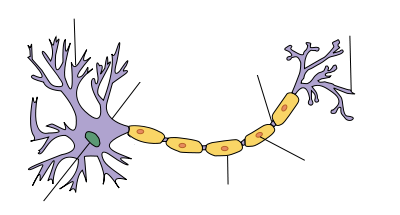
\includegraphics[width=0.9\textwidth]{images/Neuron-no_labels2.png}
    \caption{Soma and dendrites}
    \label{fig:soma and dendrites}
\end{figure}

Each nerve cell has an out outgoing axon but a cortical neuron receives input from around $10000$ synapses \cite{laughlin2003communication}\todo{check have checked laughlin check someone else, the reference for the upper number being 10000 is Lisman}.
Although synaptic numbers vary over time the number of synapses in the human neo-cortex has been estimated to be $1.5 \times 10^{-14}$ (0.15 quadrillion).\cite{pakkenberg2003aging}A synapse connects a presynaptic neuron and a postsynaptic cell across the synaptic cleft \cite{sudhof2012presynaptic}. The synapse is made up of proteins that self organise into macro-molecular machines that are responsible for signal transduction and processing.\cite{frank2016nmda}\todo{ref}  An essential function of the nerve cell is to integrate incoming information from the dendrites into a binary response at the axon.\cite{lassek2015synaptic} \cite{pocklington2006proteomes}

 The majority of synapses in the brain belong either to the excitatory glutamate system or the inhibitory GABA system. The most common type of synapse and neurotransmitter are the glutamatergic excitatory transmitters which comprise the main information processing system in the brain \cite{stewart2014structure} \todo{check ref}.

\subsubsection{History}
The term synapse, from the Greek ``to clasp together" was coined by Sherrington in 1897 writing in Foster’s textbook of physiology   Sherrington \cite{foster1895text} Since Cajal the principle model of the nervous system was of a structure composed of nerve cells built into higher order circuits. Prior to Cajal the brain was thought to be a syncytium. Cognitive complexity was thought to arise from an increasing number of connections.\todo{expand this section} 

\subsection{Molecular genetic revolution}
 Until relatively recently the synapse was thought to have a relatively simple structure controlled by a limited number of proteins and it was in the main a passive barrier across which neurotransmitters diffused.\cite{grant2019synapse}, \cite{lisman1994cam}  The brains functional unit was felt to the neural circuit and brain complexity arose from their pattern of connections. Synaptic function was limited to transferring information and maintaining a connection strength. This is not unreasonable as simple models of neurons can carry out complex calculations although they require weights at their connections analogous to synapses. This concurred with the model of learning which was that off increasing synaptic strength formalised by Hebb \cite{hebb1949organization_check}.
 
 Molecular interrogation of synaptic proteins became possible from 1992 with murine models. It was possible to catalogue synaptic proteins and clarify their function using knockdowns.  \cite{grant1992impaired}\cite{silva1992impaired}.  With the revolution in molecular genetics it was possible to characterise synaptic proteins. In 2000 Husi et al \cite{husi2000proteomic} identified 77 proteins in the NMDA receptor complex (NRC). In the next 5 years the number of synaptic proteins increased significantly, in 2006 an analysis considered the network of 186 proteins in the NRC-MASC complex \cite{pocklington2006proteomes}. The number of proteins in the post synaptic proteome as a whole had risen to 1124 in 2006\cite{collins2006molecular}.
 
 It soon became apparent that there were a very large number of proteins in the synapse and the synapse rather than simply being a gap for information transfer or a relay station was vitally involved in signal processing and computation as well as transduction. The number and combinatorial complexity of the proteins suggest an excess over what would be required for simply a connection weight.  Since 2000 the number of proteins found in synapses has greatly increased and it is now thought that there are over 3000 in the human although this number appears to be saturating. \cite{heil2018systems} \todo{query move this bit} The proteins that form the structure of the post synaptic area are modular and form higher order complexes\cite{pocklington2006proteomes}\cite{zhu2016mechanistic}\cite{frank2016nmda}.

\begin{figure}
    \centering
    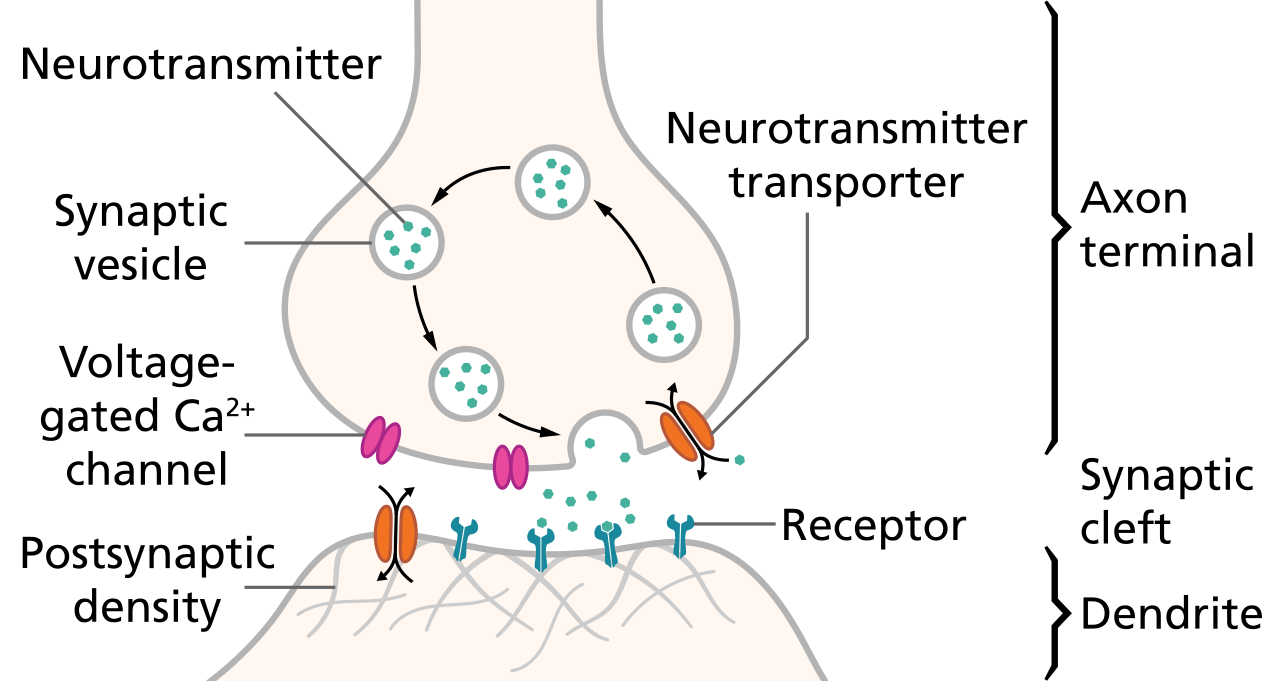
\includegraphics[width=0.9\textwidth]{images/SynapseSchematic_en.png}
    \caption{Schematic representation of synapse showing presynaptic area (labelled axon terminal) containing vesicles rich in neurotransmitters. Picture credit Thomas Splettestoesser Creative Commons \url{https://commons.wikimedia.org/wiki/User:Splette}}
    \label{fig:synapse}
\end{figure}



\subsection{Role in disease}
 

Bayes \cite{bayes2011characterization} identified 1461 proteins in human neocortical biopsies of the human post synaptic density (hPSD) and 748 that were consistent across three replicates. Using the Online Mendelian Inheritance in Man (OMIN) database \cite{hamosh2005online} and limiting the analysis to monogenic diseases the authors showed 269 diseases resulted from mutations in 199 hPSD genes and that 133 were primary nervous system disorders. Synapses are the source of action of many effective neuropsychiatric drugs and are central to putative disease mechanisms in psychiatric disorders \cite{thompson2015excitatory}, \cite{hu2015glutamate}. Also several psychotropic drugs with effects upon mood and perception have their mechanism of action at the synapse \cite{korpi2015mechanisms} as do other factors impacting on cognition and psychiatric health \cite{bocarsly2015obesity}. Reviews by Pocklington \cite{pocklington2014synapse} and Hall \cite{hall2015genetic} document convergent evidence for the importance of synaptic dysfunction in the aetiology of schizophrenia. 
The post synaptic density is the micro-molecular structure most implicated in neuropsychiatric disorders \cite{grant2012synaptopathies}. Evidence of its role in schizophrenia was found by\cite{focking2015proteomic} using proteomic studies of human brains. The evidence implicating the PSD, in particular the NMDA receptor complex, in exome sequencing of patients with schizophrenia is reviewed by Hall \cite{hall2015genetic}. Purcell et al. \cite{purcell2014polygenic} discuss the role of ARC proteins and calcium transport in schizophrenia. 
There is also evidence to suggest a role for glutamatergic signalling in Major Depressive Disorder (MDD).\cite{murrough2017targeting} \cite{de2017genetic}The anaesthetic ketamine has been extensively reported as having rapid onset efficacy in treatment of MDD. 

\subsubsection{High level function}

An important function of the synapse is controlling the strength of connections and cells that repeatedly fire at the same time are found to have strengthened connections (Hebbian learning)\cite{hebb1949organization_check}\todo{check ref. varies in references 1947 and 1949}. The discovery of long term potentiation by Bliss and Lomo \cite{bliss1973long} ultimately led to the discovery of the importance of glutamate transmission in LTP and the effect of disruption of synaptic proteins leads to a reduction in LTP and in learning
\todo{add in here or move from elsewhere the SG LTP heretical stuff}
A necessary component of adaptive neural information processing is modulating the ‘gain’ in signal from individual dendrites by controlling the strength of the connections between neurons. The synapse can do this through the processes of short and long term potentiation. Classical Hebbian \cite{hebb1949organization_check} long term conditioning requires the arrival of the signal at the presynaptic terminal, and postsynaptic depolarisation leads to a strengthening of connections.   Hebb posited a model where the strength of a connection between two neurons depends on how often they are activated together and as neural circuits determine behaviour these patterns of activation are then learned. Hebbian learning remains a fruitful model for computational models of learning. 

\section{Synapse structure}
The synapse is composed of a presynaptic area filled with neurotransmitter vesicles, a gap or cleft between the presynaptic areas and the post synaptic area and a post synaptic area containing neurotransmitter receptors and structural proteins. Nerve signals arrive at the presynaptic area, cause release of neurotransmitters from synaptic vesicles which diffuse across the cleft and are detected by post synaptic receptors whose activation may lead to depolarisation of the cell axon. 


\subsection{Presynaptic area}
The presynaptic area is separated from the post synapse by the synaptic cleft \cite{rusakov2011shaping}.  The synaptic cleft is approximately 20nm in size \cite{zuber2005mammalian}\todo{fix missing circumflex in first name of zuber} and is spanned by trans synaptic adhesion molecules.  \cite{missler2012synaptic}


 The presynapytic area contains neurotransmitters stored in vesicles which are docked and fuse with the plasma membrane at a specialised active zone an electron dense area , parallel to and juxtaposed to the plasma membrane.\cite{schoch2006molecular}. Neurotransmitters are substances which when they diffuse across the synaptic cleft give rise to signal in post synaptic receptor. Active vesicles are docked at the edge of the membrane and released following calcium influx. \cite{lassek2015synaptic}. After neurotransmitter release the vesicle is recycled by endocytosis.\cite{ashery2014molecular}
 
 Vesicles are primed by a protein complex consisting of 5 evolutionarily  conserved proteins acting as a complex RIM, Munc13, $\alpha$-liprin, RIM BP and ELKS proteins. \cite{sudhof2012presynaptic}. Piccolo and bassoon proteins are also associated with the active zone in vertebrates.  SNARE proteins facilitate vesicular fusion. \cite{sudhof2012presynaptic}. Mitochondria \cite{lassek2014proteome} are also an integral part of the presynaptic area and are noted on the earliest examinations \cite{gray1959electron}. The active zone is closely associated with extra cellular matrix \todo{ref}.
 
   In certain nerve cells such as photo-receptors, the active zone is ribbon like and capable of prolonged discharge  \cite{ashery2014molecular}.  
 
 Neurotransmitters transform nerve impulse signals through changing their pattern of release over short time frequencies in response to specific encoding of incoming signal (short term potentiation \cite{sudhof2012presynaptic}. Along with the post synaptic area they can strengthen the signal produced by neurotransmission over longer time scales (long term potentiation). A substantial amount of neural computation occurs in the presynaptic area and is dependent on synaptic proteins \cite{sudhof2012presynaptic}.
 
The presynaptic area developed from vesicle transport systems in earlier organisms and has developed more recently than the PSD.\cite{emes2012evolution}
 



\subsection{The post synaptic area and post synaptic density}

The post synaptic density (PSD) is an electron dense area parallel to the synaptic plasma membrane extending $\approx$ 35nm deep to the plasma membrane.\cite{harris2012ultrastructure} Formed from structural proteins that bind to actin in dendritic spines, and also to the receptor complexes, it contains protein kinases, receptor molecules and protein scaffold complexes such as PSD95. There are slight differences in its composition between mouse and man \cite{bayes2012comparative}, but in general its component structures are conserved in vertebrates.

Signal transfer across the synaptic cleft is typically mediated by neurotransmitter chemicals although direct electrical transmission can occur across gap junctions in the retina and in locations in the central nervous system.  \cite{stewart2014structure}\todo{cited by 11 see if we can find a better reference}. The neurotransmitter receptors are both held in place and modified by protein complexes such as guanylate kinases (MAGUK) that include glutamate receptors, and organise proteins involved in synaptic plasticity \cite{zhu2016mechanistic}. The release of glutamate is closely aligned with glutamate receptors in the post synaptic density (PSD). \cite{harris2012ultrastructure}

 The receptors in the post synaptic density show a geographical variation with the  $\alpha$-amino-3-hydroxy-5-methyl-4-isoxazolepropionic acid  receptors (AMPAR) and N-methyl D aspartate (NMDA) receptors in close apposition to the presynaptic active zone and the metabotropic glutamate receptors (mGluR) receptors in the peri-synaptic zone.\cite{scheefhals2018functional} 
 
 The ionotropic receptors have the fastest signalling characteristics and include NMDAR, AMPAR and Kainate receptors (KAR) named after the particular agonists found to provoke them.\todo{ref} Kainate acid receptors have a metabotropic G protein mediated element in their response and are less involved in synaptic transmission \cite{contractor2011kainate} than the two pure ligand gated inotropic receptors NMDAR and AMPAR.  The metabotropic glutamate receptor works through the mediation of g proteins and results in signalling and also recruitment of further ionotropic receptors to the post synaptic area.\todo{ref} \todo{does this not belong with the section~\ref{sec:Neurotransmitters} }
 
 The post synaptic density is the most evolutionarily ancient part of the synapse with its components arising in prokaryotes\cite{grant2018synapse} \cite{emes2012evolution}. 


The post synaptic proteins show many remarkable features. First they are relatively resistant to complete abolition of function.Even in knockout animals some signalling remains showing a degree of robustness, also dysfunction of many disparate elements result in common phenotypes particularly neuropsychiatric phenotypes. A very wide variety of mutations at different proteins and different loci within specific proteins can give rise to common disorders such as ASD. By contradistinction point mutations in key receptor proteins tend to give rise to severe phenotypes as we shall see later but also give rise to different phenotypes from mutations at different points in the protein (a case in point here being grin2a).

PSD proteins form into supercomplexes. 





\subsection{Molecular function}
Calcium ion influx is necessary for depolarisation. Synaptotagmin acts as a calcium sensor and allows for rapid fusion of synaptic vesicles with the cell membrane and release of neurotransmitters into the synaptic cleft.\cite{martens2007synaptotagmin}  It is also necessary for  learning in animals and long term potentiation and depression \cite{lisman2012mechanisms}.
\subsubsection{Neurotransmitters}
\label{sec:Neurotransmitters}
L glutamate , a small amino acid, is the dominant neurotransmitter at excitatory synapses within the brain \cite{niswender2010metabotropic}. Fast excitatory neurotransmission is carried out at the ionotropic glutamate receptors AMPA and NMDA \cite{traynelis2010glutamate}. Ionotropic glutamate receptors consist of 4 sub-units spanning the extracellular membrane that form a central ion pore. AMPA and Kainate receptors are homo or heterotetrameric but the NMDA receptor is obligatory heterotetrameric. The AMPA receptor is responsible for most of the fast excitatory transmission in the central nervous system \cite{henley2013ampa}. It is composed of four sub-units GRIA1-4 and is mainly permeable to sodium (Na+) and potassium (k) ions. The glutamate receptor sub-units originate from 18 different gene protein products representing NMDA, AMPA, Kainate and delta groups \cite{traynelis2010glutamate}. The NMDA receptor is also composed of four subunits (a tetrameter)  but is permeable to calcium ions. AMPA and KAR are fast acting working in less than 1ms \cite{traynelis2010glutamate} NMDAR depolarise more slowly in the 10ms range (cite neuron paper) 

Magnesium (Mg$^{2+}$) ions initially block NMDA receptor activity and  AMPA receptor activation is required to displace the Mg$^{2+}$ ions. AMPA is closely involved in long term potentiation. After Ca$^{2+}$ ion entry from the synaptic cleft, CAMKII is activated and leads to an increase in AMPA receptors at the post synaptic membrane.Calcium can entry through NMDA receptors after unblockage of Mg ions and its entry leads to activation of Calcium/Calmodulin dependent protein kinase. The kinase subsequently binds to NMDA receptors and phosphorylates sub-units of the AMPA type glutamate receptor.

Slow synaptic transmission, mediated by G protein second messengers, results from the action of metabotropic glutamate receptors \cite{niswender2010metabotropic} although mGluR signalling can also occur in time scales closer to igluR. There are eight mGluR subtypes. Metabotropic glutamate receptors are family C G Protein coupled receptors (GPCR). Group 1 mGLU promote intracellular calcium release whereas 2 are localised pre and post synaptically  and 3 are localised presynaptically \cite{niswender2010metabotropic} \footnote{grm 2,3,7 in group 5 - 2 and 3 are in group 2 , 7 along with 4,6,7,8 are om group 3, (grm 1 and 5 are group1), 1,2,3,5 and 7 are in the PSP, 1 is in 22 and 5 in group 32 - groups 20, 22 and 32 are quite closely related see \url{ source('~/RProjects/graph_groups/R/distribution_m_glu_glutamate.R')}Group II Metabotropic Glutamate Receptors Mediate Presynaptic Inhibition of Excitatory Transmission in Pyramidal Neurons of the Human Cerebral Cortex shows can be pre and post synaptic } but there is also evidence for pre and post synaptic action \todo{? more to discussion}
Metabotropic glutamaate receptors exert their effect by increases in protein synthesis Group II have been related to anxiety scz and alzheimers disease( Swanson) .
Glutamate levels are kept controlled by the glutamate glutathione pathway and glutamate transporters. 

\subsubsection{Long term potentiation}
Periods of synaptic activity can increase the strength of synaptic connections by the process of long term potentiation (LTP).

The theory that an increase in the strength of connection between neural cells leads to learning was first proposed by Cajal in 1911 \cite{nicoll2017brief}. Hebb proposed a model where there is synaptic modification following coextant pre and post synaptic activation \cite{hebb1949organization_check}. Later tetanic stimulation of rabbit hippocampal synapses was shown to result in an increase in the subsequnet strength of these responses.\cite{bliss1973long} NMDAR activity was subsequently shown to be necessary for LTP \cite{collingridge1983excitatory} but not for neurotransmission. 
 Interfering in the process of LTP in animal models leads to defects in memory and learning \cite{lisman2012mechanisms}).
 \cite{lisman2017glutamatergic} makes a connection between the modular structure of the synapse and the variety of potentiation responses.\todo{read this paper}`. The composition of the synapse into 70-80nm modules of independently activating AMPA receptors explains many problems with forms of plasticity.
 Six different forms of plasticity are observed in the synapse short term plasticity, long term plasticity, late long term plasticity, long term depression, distance dependent scaling and homeostatic scaling \cite{lisman2017glutamatergic}. Short term mpotentiation reuslts from weak stimuli and occurs early and is a promising model of working memory as GluA1 knockdown animals have abormal STP and long term memory. Early LTP is likely mediated by phospohrylation of GluA1 by CAMkII. Late long term potentiation is associated with a change in the size of the PSD. LTP is axiomatically defined as beginning 30 mins after a tetanic stimulus. Late LTP as associated with more AMPAR signalling with recruitment to the synapse and an increase in quantal probability. This often requires other factors such as dopamine in CA1 and BDNF and has been referred to as NeoHebbian. The mechanisms of this late stage include first increase in receptors from PSD 95 mediated \todo{check} CAMKII phosphorylation of stargazin or of syngap or activation of erk kinase through syngap. 
 MOdelling of the synapse suggests that responses can be explained if there are hotspots where there are either modules of AMPA receptor present or absent on vesicle release and plasticity can occur with recruitment to silent hotspots. \todo{network effects from this bit}
 
 
\subsection{The synaptogenic model of neural plasticity}


An alternative model of synaptic learning has been proposed that takes into account the level of synaptic complexity. In this model temporal neural signals are distributed according to the organisation of synaptic proteins into complexes and supercomplexes with specific combinations of elements attuned to particular temporal responses and then mapping to different areas in the brain. 

There are a number of reasons that the synaptic weight hypothesis may be incomplete, increases in LTP accompanied by difficulties in learning, very specific behavioural phenotypes from synaptic variation but without evidence of a circuit based change. 

 In contrast he suggests a bottom up synaptogenic model in which the synaptic protein composition acts as a zip code which allows spatially distributed neurons to respond to particular patterns of receptor stimulation. In support of his arguments he points out that the association of long term potentiation with learning remains controversial and it may be that the glutamate receptor (NMDA both subsume LTP and learning rather than affecting LTP which in turn causes learning. An example suggesting this is that mutations in PSD 95 give rise to cognitive impairments but increased long term potentiation.

\subsubsection{Analogy with synaptic models of computation}
\todo{commented out areas here may want to keep some of these}
% As regards the model of a bottom up approach to the structure of the synapse and behaviour we will adopt a similar approach seeking groupings of proteins and hence their cognate genes and seeing what their effect are on population studies of cognitive differences, enrichment for murine models of cognition or their role in disorders with a cognitive phenotype. Our approach however is looking for enrichment in-silico rather than in changes in behaviours of experimental model organisms. 

% One area I should mention here is that there is a middle ground between the one circuit one behaviour model with weights and a distributed bottom up model with an intrinsic frequency response. Primitive models of the synapse prove to be powerful computational devices. One of Grants arguments is that the synapse is a computational unit. A group of connected neurons with associated weights can give rise to complex decision making behaviour by allowing representation of structures being learned to be encoded as patterns more proximally in the network without there being a specific circuit for each response (for example in MNIST there is not a pattern of activation that is specific to 1 or 2 there are patterns of activation that are more likely to result in the final soft-max function choosing one of these) I would speculate that the combination of weights and circuits and the enormous complexity of the synapse allows to some extent the complex cognitive computations carried out by mammals particularly those in areas of locomotion and sensation that have proved so hard to simulate.
\subsection{Importance}

There are many reasons to be interested in synaptic function but I consider five to be of particular importance. 

First, synapses are involved in the overwhelming proportion of neuropsychiatric disorders \cite{grant2012synaptopathies}.  Second, they are composed of a large  number of proteins, many of which have roles outside of the nervous system and are an attractive basis to understand the genetics of complex cognitive traits, involving generalist genes, many of which exhibit significant pleiotropy \cite{sharma2000induction}\cite{plomin2015genetics}. Third, the synapse has proved a useful practical model of information processing and simplified models of the synapse have been able to carry out powerful computations \cite{hinton2007learning}, \cite{dean2012three}. However the synapse is considerable more complex than the simple weight used in these models. Fourth, synapses are the building blocks of higher levels of brain structures \cite{armstrong2012evolution} and will likely affect their function \cite{dean2012three}.

Finally they provide a molecular basis for human learning and memory \cite{kandel2014molecular},\cite{gallistel2013neuroscience}.
\section{The synapse}



      



\subsection{Evolution}


The presynaptic density has evolved earlier in evolution than the post synaptic density and is present from the time of the vertebrate expansion of the synaptic proteome. By contrast the PSP is more evolutionarily ancient. The proteins composing it are found in the earliest yeasts. The new proteins found in the mammalian PSP are the result of paralogue expansion. The PSP originated in the sensory signalling complexes of bacteria. These are too small to detect a difference in chemical gradient along their length and therefore Grant hypothesises that the function of these earliest receptors was to detect differences in chemical composition of their environment swim and then check again the composition of the environment. From this he concludes that the earliest function of the PSP is in recording differential pattern to the time course of signals arising in the organism. The presynaptic area is derived from endocytosis related mechanisms.

A genome duplication event approximately 550 Ma ago led to a significant increase in synaptic complexity \cite{nithianantharajah2013synaptic} , \cite{grant2016molecular}.

\todo{Cite those from extra bib also ? cite the Hill paper on evolutionary conservation much of this could go next to the pLI bit
}

Hill combined data from CHARGE and someone else to show using Linkage dysequlibrium regression. LD regression that areas of the genome enriched for SNPs associated with differences in intelligence were under negative evolutionary pressure finding these regions contained 2.6\% of SNPs but ~40\% of SNP based heritability. \cite{hill2016molecular} 

Networks as well as reduplication can provide robustness



 

\subsection{Systems Biology approaches to the synapse}

Systems biology entrails knowledge of the structure and dynamics of a biological system as a whole as well as its composite parts \cite{kitano2002systems}. System behaviour can differ from that of component parts and considering system structure, system dynamics, the control method and the design principle can help to understand these differences \cite{kitano2002systems}. Complex systems can be compactly represented as networks (section~\ref{sec:networks_intro}) and their structure analysed using algorithms derived from graph theory. Advances in computation, databases and ontologies improve our ability to understand , model and reason about these systems. 
 
\subsection{Models of the synapse}

Initial yeast models of the synapse were of poor quality so data mining of the literature for interactions was required to develop effective and comprehensive static models \cite{pocklington2006proteomes},\cite{armstrong2012evolution}. Databases are now of better quality and use standardised ontologies to organise their information)\cite{brazma2006standards}, \cite{hermjakob2004hupo}, \cite{kerrien2007broadening}. Databases however contain evidence on interactions that are less likely to be valid than evidence of direct experimental, interaction (eg literature data mining and co-expression). In order to develop a useful model of synaptic interactions, a significant amount of data cleaning, organisation and transformation of these databases is still required. This review will concern models where the interactions are inferred from experimental evidence of direct interaction in mouse or human. Synaptic components are purified using centrifugation and protein components examined by mass spectrometry. The process is reviewed in depth by \cite{lassek2014proteome} A comprehensive review of systems biology models of the synapse and their development is provided by Armstrong and Sorokina (2012). \cite{armstrong2012evolution}

\subsection{Static methods}

Protein-protein interactions in the synapse can be represented as an interaction graph with dots (vertices) representing the proteins and an edge connecting the vertices if the proteins interact. Alternatively the gene that encodes the protein product may be used. This is helpful if we wish either to annotate the structure with results from the biomedical or experimental literature, or to use the graph structure to better understand results from population molecular genetics. 

\subsection{Dynamic models}

Synapses can be modelled as dynamic entities with interactions between components and specific location, stoichiometric and kinetic constraints. Two common types are those based on systems of partial differential equations or agent based models. \cite{sorokina2013simulator},\cite{sorokin2014rkappa}, \cite{walpole2013multiscale}.

Although this thesis will not address dynamic models the interaction logic of the static model is essential for the generation of dynamic models. In addition if we discover structures within the network that have an enriched association with animal or population genetic models of cognition these will be fruitful areas for future dynamic simulation. 

\subsection{Finding communities in protein protein interactions}
Advances in molecular biology have increased our understanding of the function of the synapse and of its constituents. Initially the synapse was thought to be a relatively simple structure with few components but now there appear to be over 3000 proteins whose interactions are important for synaptic function. In addition there is a core of around 1000 proteins that are conserved across mammalian lines.  Protein interactions form macromolecular machines and the interconnections of proteins are vital to the function of the synapse. 
Synaptic proteins form modular structures \cite{pocklington2006proteomes} and there is evidence that the composition of these complexes are ‘optimally tuned’ for normal function \cite{grant2012synaptopathies}. Identifying and studying these large scale structures in the network may help in understanding the role of synaptic components in complex traits and neuropsychiatric disease.




\subsubsection{This is a bit about networks}
We have therefore a very complex wiring diagram of the synapse but we still don’t know what are its natural units and how the network structure of the synapse affects complex traits is unknown. One way to represent complex systems interactions is as a network. The burgeoning field of network science has made great advances this century and uses advances from graph theory, computer algorithms and statistical physics. Network theory allows the interrogation of the function of complex systems in terms of the pattern of their interconnections and shows common functional consequences of particular structures across disparate forms of network for example the internet, social networks and protein protein interactions. In this thesis I will show how an understanding of synaptic structure can help us to understand the molecular genetics of a complex trait in this case genetic differences in cognitive ability. I will also use the example of cognitive ability as a proof of concept of how these techniques can be used to understand neuropsychiatric disorders. Network approaches to disease

\subsection{Previous network based GSA}

\todo{citation error - could simply be that it is missing from the references}
\todo{PhD specific bibliography}
\cite{nguyen2018network}    review the use of pathway gsa for 36 packages.
Extends tools to 2017. If a package is not easy to use it will not be used by life scientists. Our approach makes use of commonly available GSEA and MAGMA packages and requires only editing of .gmt files which we provide software for. Of 45 packages, 30 were standalone or web based. They note that only one package is HIPPA compliant with web tools. Lots of the packages are implemented in R. Variety of ways in which information can be put in. If using list of genes this involves a cut off which involves loss of information. Discusses three different types of pathway signalling pathway, metabolic pathways and PPI. They note that SPIA accepts adjacency matrix representing a directed graph. Two types of graph models, single where a node is one thing and multiple. Topology GSA allows the graph to be split into sub graphs.
Then they discuss pathway scoring methods and the goal of producing a ranked list of pathways or sub-pathways.

\todo{Perhaps I should mention the use of david}

\subsection{Others not covered in this review}
Ghissian et al \cite{ghiassian2015disease}. There also appear to be other papers by Ghissian including on endophenotype. So for review this is the one where they use Louvain clustering on a generic network (? string) and find not \cite{blondel2008fast}so much but they fuind that the clustering of disease related genes together is greater than chance. he increasing evidence of the role of protein complexes mediating synaptic plasticity in schizophrenia.

The network can be analysed at the level of overall network, of an individual node or at the level of structures found within the network and I will discuss each of these with relation to cognitive ability. I will describe our experience of a pilot study and the reasons for choosing cognitive ability. I will also introduce and review the network analysis techniques that we utilised. 
 






\section{Intelligence}

\subsection{Measures and heritability}

People differ in their cognitive abilities and their ability to solve mental problems. The approaches to testing intelligence or cognitive abilities have been informed by function or lesion studies in the neuroscience community and on correlation between disparate tests revealing latent factors in the differential psychology literature \cite{deary2014stability} (Deary, 2014).

Given a number of different tests of cognitive ability individuals who do well on one test will tend to do well on others, and hence there will be a correlation between these results. This correlation between performance over several categories is the general intelligence factor, g or ‘general intelligence’, described by Spearman in 1904  \cite{deary2001intelligence}(Deary,2001), \cite{deary2014stability}. This construct accounts for about half the variance in individual cognitive performances \cite{deary2009genetic}(Deary et al 2009). The g factor can be discovered from a variety of disparate cognitive tests using principal component or factor analysis or by using cognitive tests that ‘load highly on the general cognitive factor’ \cite{johnson2004just}(Johnson et al. 2004), \cite{deary2009genetic} (Deary et al 2009).

As well as general cognitive ability (g), there is a positive correlation in performance on similar tests that relate to factors representing cognitive domains such as memory, processing speed, vocabulary, reasoning and spatial ability \cite{deary2010cognitive}(Deary et al 2010). In addition crystallized intelligence (gc) and fluid intelligence (gf), identified as factors of g by Cattell and Horn, change at different rates over the life course. Crystallized intelligence is composed of features such as knowledge of facts, vocabulary and certain number skills and does not tend to deteriorated until old age in contrast with fluid intelligence which requires ‘on the spot processing’ \cite{deary2010cognitive}(Deary et al 2010),\cite{davies2015genetic} (Davies et al 2015).
The heritability of cognitive abilities has long been recognised since Galton (1865). The genetic influence on human intelligence has been estimated at between 30 and 80\% and the heritability of the g factor increased from 30\% in youth to 50\% in adulthood to older age \cite{deary2009genetic}(Deary et al, 2009). 
Cognitive ability is an attractive complex cognitive trait to investigate using a structural model of the synapse. It is highly heritable and we know that a large proportion of its heritability can be marked by single nucleotide polymorphisms. In addition it can be reliable measured quantitatively; has a positive as well as a negative extreme, and is normally distributed \cite{plomin2015genetics}(Plomin and Deary 2014). Finally we have evidence that synaptic components are involved in variations in human cognitive abilities. 

The fact that this trait is normally distributed with a positive as well as negative extreme is attractive as it reduces the effect of hub centrality lethality effects on essential genes resulting in severe effects but not directly relating to their function \cite{jeong2001lethality}(Jeong et al 2001). Hubs, genes or proteins with large numbers of connections to other nodes are disproportionately involved in severe phenotypes but less so in complex and polygenic traits \cite{bayes2011characterization}(Barabasi et al 2011a) Analyses of communities in network models of the synapse therefore frequently yield associations with cognition (particularly when testing for over representation of terms in the biomdedical literature) due to mutations of these genes producing pjenotype that are associated with severe intellectual disability or non viability in animal models. Pocklington et al \cite{pocklington2006proteomes} (2006a) found that intellectual disability, unlike other neuropsychiatric disorders associated with cognition were widespread in the genome and through the clusters tha he identified in the MASC complex.

Intelligence is stable over the lifespan, both in terms of the average of the measure and rank. The correlation is about 0.7 but may be higher as the full range of those tested are not seen in follow up \cite{deary2009genetic}(Deary et al, 2009). Those of higher intelligence do not have better cognitive ageing but are more likely to have habits such as exercise and education that predispose to successful cognitive ageing \cite{deary2014stability}(Deary, 2014). 

Twin studies (Deary et al 2009)\cite{deary2009genetic} show greater correlation in changes in cognitive ability over a lifetime for monozygotic than dizygotic twins.

\subsection{Cognitive epidemiology}

Cognitive epidemiology is the study of intelligence as measured by psychometric tests – as an associated of mortality, illness and health (Deary, 2010)\cite{deary2010cognitive}. The effects of differences in cognitive function in health outcomes have been recognised since the 1930s \cite{deary2007cognitive}(Deary and Batty, 2007).

A systematic review of nine cohort studies found that IQ in childhood and early adulthood was associated with lower mortality in middle and late adulthood Batty et al (2007).\cite{batty2007premorbid} Higher cognitive ability is associated with important outcomes such as educational achievement and occupational success.

It is possible that the effect on lifespan might be due to social factors that have a common effect on intelligence, but studies including and analysis of three twin registries supported a genetic effect to explain correlation between lifespan and intelligence (for example the correlation I stronger for monozygotic than dizygotic twins (Arden et al 2016).\cite{arden2016association} General cognitive function affects the incidence of psychiatric disorders (Wraw et al 2015).\cite{wraw2015intelligence} Hill et al (2015) showed, using linkage disequilibrium regression, a common effect of genetic variants on cognitive ability and mental disorders with different effects at different points in the lifecourse.\cite{hill2016age}

\subsection{The molecular basis of cognition.}

One approach to the molecular basis of cognition has been that adopted by the Gene to cognition group (Croning et al, 2009).\cite{croning2009g2cdb} This is a pathway approach of examining variations in MASC and other synaptic genes which are linked to changes in memory in experimental animals (Deary et al 2009).\cite{deary2009genetic}

Molecular genetic approaches need to determine whether there is an effect of genetics on the environment ie genetic mediating environmental change, or whether genetic effects alter individuals’ susceptibility to the effects of environment (Deary et al 2009).\cite{deary2009genetic} In addition, although less marked in recent years, genetic approaches to cognitive ability remain highly controversial. In describing a computational systems biology approach to cognition, although it may appear clear from this review, it is important to avoid the implication that this implies a computational model of mind or of cognitive abilities. 

\subsection{Genome scale molecular findings}

Until recently the largest GWA study of intelligence in children (n=18,000) found no variants of genome wide significance (Benyamin et al 2014)\cite{benyamin2014childhood}, (Plomin et al 2013)\cite{plomin2013common}. The use of educational attainment, which has a moderate correlation with intelligence, has permitted the use of large study sizes which have shown genome wide significant findings but effect sizes have been small. Recently cohorts with larger sample sizes such as CHARGE and UKBiobank have permitted the identification of variants with significant association with cognitive ability at the genome wide level. 

Genome wide complex trait analysis (GCTA) (Yang et al 2011)\cite{yang2011gcta} of GWAS studies has shown that common SNPs can account for about half the heritability found from twin studies. Davies et al (2011)\cite{davies2011genome}, using five cohorts in the Cognitive Ageing Genetics in England and Scotland (CAGE) consortium (see section 13 for further details) used GCTA (Yang et al, 2011)\cite{yang2011gcta} to estimate the proportion of crystallised and fluid cognitive ability accounted for by linkage disequilibrium (LD) between SNPs and unknown causative loci. The estimates were 51\% for fluid intelligence and 40\% for crystallised intelligence. Using data from the Cohorts for Ageing Research in Genomic Epidemiology (end p 16) (CHARGE) consortia (PSATY ET AL 2009).\cite{psaty2009cohorts} Davies et al. (2015)\cite{davies2015genetic} estimated the lower bound of the narrow sense heritability for variation in cognitive ability to be 0.29 and 0.28 from the two largest cohorts in the meta-analysis.

Davies et al (2015)\cite{davies2015genetic} found 13 SNPs of genome wide significance for cognitive ability in a meta-analysis of data from the CHARGE consortium (n= 53949) Using VEGAS to generate gene level statistics, one gene was found of genome wide significance: HMGN1. The genomic inflation factor ($\lambda=$)\todo{Complete} suggests a polygenic effect on the phenotype.

Davies et al (2016)\cite{davies2015genetic} recently reported a genome wide association of 112151 individuals from UKBiobank (Elliot and Peakman, 2008)\cite{bycroft2018uk} \cite{elliott2008uk}. The association between genotype and educational attainment and three cognitive tests: reaction time, memory, numerical reasoning was tested. Gene based statistics were calculated using MAGMA without a gene window \cite{de2015magma}(de Leeuw et al 2015a). 149 SNPs at three independent regions were significantly associated with verbal numerical reasoning. Gene based analysis identified 17 significant genes across seven genomic regions. These included genes associated with mitochondrial function (NDUFA6), septin 3 which is associated with Alzeimers disease and other genes associated with neurobiological pathways (e.g. ATXN3L). The proportion of variance explained by common genetic variants calculated by GCTA was 31\%.
For reaction time there were 36 SNPs of genome wide significance spanning two regions. 23 genes across 9 regions were found to have significant associations with reaction time. 

There were no genome wide significant SNPs for memory. 115 SNPs were identified that were associated with educational achievement. Gene based analysis identified 95 genes across 28 regions associated with educational attainment.

\subsubsection{Recent GWAS}
\todo{CTG and UKBB}
Sniekers \cite{sniekers2017genome} in 2017 reported a meta-analysis of 78308 of  individuals of European ancestry from 13 cohorts including UK Biobank (54119). 336 SNPs were discovered in 18 genetic loci. 22 Genes were implicated by gene location and MAGMA GWGWAS identified 47 genes at a genome level of significance. 17 of these were also found by SNP genetic loci. Only one gene set was found to be significant after correction for multiple comparisons GO: regulation of cell development using MAGMA GSA (adjusted p=0.03, p=$3.5 \times 10^{-6})$.\cite{de2015magma} The authors note that the four next most significant gene sets (although not significant after correcting an $\alpha$ level of 0.05 for multiple comparisons) are related to neural function. The authors report that 14 of 44 genes which had data from the GTEx consortium were differentially expressed in the brain.\cite{gtex2015genotype}.Further analysis by combining this data with high intelligence cohorts is described \cite{coleman2019biological}.

Hill \cite{hill2019combined} used multi trait analysis of genome wide association studies using summary statistics MTAG\cite{turley2018multi} to increase sample size to 248 482 from 199 242. They included summary statistics from Sniekers (n=78,308)\cite{sniekers2017genome} and the study of educational attainment by Okbay (n=329417). These were augmented using 120934 new UK Biobank participants (UK Biobank Participants in the other studies contributing to the analysis being excluded). The new UK Biobank participants from this study will be used for analysis in this thesis as Intelligence\textsubscript{Discovery} cohort. 

They found 187 genetic loci associated with intelligence involving 538 genes. Gene set analysis using MAGMA revealed enrichment for 7 pathways incluiding  neurogenesis, regulation of nervous system development, regulation of cell development, neuron projection, central nervous system neuron differentiation, synapse \textcolor{red}{significantly for us}, neuron differentiation and oligodendrocyte differentiation. 

Savage \cite{savage2018genome} reported in 2018 a meta analysis of 14 different studies of general intelligence. This was again dominated by UK Biobank n=195653) with a significasnt contribution from COGENT. They reported 205 genomic loci and 1016 involved genes of which 939 were novel. 

There are reviewed by Plomin and Stumm\cite{plomin2018new}.

\subsection{Educational attainment}
\label{sec:Intro Educational Attainment}

The use of educational attainment as a proxy for intelligence has allowed a great expansion in sample size in GWA studies \cite{plomin2018new} as educational attainment is routinely reported in a number of social science and other GWA. The correlation between educational attainment and intelligence is phenotypically 0.5 and genotypically 0.65 in a review articles by Plomin. \cite{plomin2018new} citing  \cite{rietveld2014common}. In their report of a meta-analytic GWAS of intelligence Sniekers et al used LD score regression to calculate the correlation of their sample with 14 traits.\cite{sniekers2017genome},\cite{bulik2015ld}. The strongest assocation was with educational attainment (r\textsubscript{g}=0.70).

Rietveld et al (2013) \cite{rietveld2013gwas} looked at educational attainment as a proxy for cognitive ability. He used a meta anlysis of GWA studies examining the binary variable of college attendance, and regressed the number of years of education against the genotype (Rietveld et al 2013c). The discovery sample was 101,069 individuals, and the replication cohort 24,490 individuals. A total of 126599 individuals underwent genotyping and summary SNP data has been made available on the Social Science Genetic Association Consortium (educational attainment) website http://www.thessgac.org/!data/kuzq8. Rietveld et al (2013c) found three SNPs of genome wide significance, and all measured SNPs accounted for 2\% in the variance of outcome.\cite{rietveld2013gwas}

Okbay et al \cite{okbay2016genome}(2016b) reported 74 loci associated with educational attainment in an expansion of the cohort used by Rietveld The discovery cohort was now 293723 individuals in size and the replication cohort carried out on UK Biobank, 101,069. Gene set analysis showed enrichment for synaptic components particularly SHANK2. (pg18)

The largest educational attainment study to date is of 1.1 million individuals \cite{lee2018gene} The study was conducted using years of education as a phenotype in individuals of european ancestry. The authors identify 1271 independent genome wide SNPs. The authors were able to explain 11\% of educational attainment vairance using a polygenic risk score \cite{lee2018gene} \todo{this is quite close to the original although cited}. Using DEPICT they were able to show enrichment for pathways involved in the nervous system. The authors performed an analysis to support their depict findings using MAGMA GSA, interestingly they used a 5kB window around genes.  

Plomin (new) \cite{plomin2018new} box 5 makes the point about the availability of summary statistics and the non availability of some from commercial enterprises an observation which I completely agree with maybe should move to discussion.

\subsubsection{Recent GWA}
UKBB Ed and EA2 and overlap between and EA3

\subsection{Relevance to the systems neuroscience of the synapse}

The genetic architecture of differences in cognitive ability as of all complex traits, (to the extend that we can extrapolate from current studies), is that the genetic contribution to the phenotype is from many genes of small effect (Plomin and Deary 2014). In addition many of these genes are pleomorphic, shown by their association with health outcomes (Deary, 2008) and psychiatric morbidity (Hill et al, 2015). We have seen evidence that genes encoding synaptic proteins may be associated with cognitive ability and educational attainment (Hill et al 2014), (Okbay et al, 2016a).

Intelligence as the manifestation of the integrated function of neural systems is ‘central’ to systems neuroscience approaches (Plomin and Deary 2014), (Deary, 200). Network studies as we have discussed earlier, have implicated subsets of synaptic genes in intellectual disability and disorders with a cognitive phenotype (Pocklington et al, 2014), (Pocklington et al 2006a), (McLean et al. 2016). There is compelling evidence that the genetic effects on complex traits may be medicated by communities of genes (Barabasi et al, 2011a). I will discuss later (section 7.4) how network structure might allowed a relaxation of constraint in variation amongst many synaptic genes to produce a complex, continuous rather than severe phenotype.

I will describe a quantitative method that uses the large scale structure of networks to identify many genes of small effect which, acting in concert, may have an effect on cognitive ability. I will now consider how we can generate these communities before turing to the issue of how we will tedst their association with cognitive phenotypes.


We can extend this to multiple groups by recursively partitioning the network based on the leading eigenvector of the partiion and stopping partitioning when the partition does not result in a further increase in the modularity for the subdivision of the community (see Newman (2006) for further degtails). This is the method implemented by McLean et al (2016)

\subsection{Usefulness of intelligence as phenotype}

Before going on to discuss the methods that we can use to identify coherent sets of genes in a network we should point out that one of trhe aims of the study is to assess how well network analysis and clustering helps in the understanding of a phenotype. If the phenotype is poorly defined or their is a great deal of inter observed variability it may be that the clustering is measuring the phenotype (for example finding an unexpected subgroup of the phenotype) rather than assessing the effectiveness of modules of proteins associated with the phenotype.

\section{Gene level tests}
\todo{Keep this introduction bit and then move the bit on specific methods to a methods section perhaps start of chapter 2 do the same with the bit at the start of GSA}
Genome wide association studies test the association of single nucleotide polymorphisms with a phenotype.\todo{ref}
In order to test hypotheses about the importance of network structures in the post synaptic proteome to a phenotype we will need to perform significance tests for a group of genes. In order to test whether the properties of individual vertices in the network such as degree are associated with the phenotype we will need a statistic that measures the association of the vertex with the phenotype.  

It is necessary therefore to have a statistic for the significance of the association of a gene encoding a protein in the synaptome with a phenotype. This will require assigning SNPs to genes and generating a combined statistic (Petterson et al 2011).

Several authors have described methods for generating gene level association statistics. It has several attractions. For one the number of statistical tests in doing inference is reduced from over 500,000 for SNPs to approximately 20,000 for gene level tests with a commensurate reduction in the penalty for multiple testing. In addition genes are a natural biological unit and can be used in models of networks, proteins and other biological entities. Any form of pathway analysis will depend on finding a way of producing gene level statistics that are computationally tractable, reliable, repeatable and in which the analysis can easily be reproduced. As this will form the basis of our interrogation of networks, it is important that these foundations are sound. Given the lack of reproducibility in some computational approaches, particularly within network and pathway studies (Mitrea et al 2013b), we wish to ensure we can compare our findings with published work given a specific set of GWAS results.
% This is rather problematic as many authors have used the WTCCC Crohns dataset to test simulations including de Leeuw et al (2015b), de Leeuw et al (2016), Li et al (2012), Li et al (2011) and Kwak and Pan(2015). Unfortunately this data is not available for donwload from the WTCCC website at present and when I wrote to the WTCCC they confirmed to me it was unavailable. 
Rietveld et al (2013c) reported gene level statistics for educational attainment using VEGAS and VEGAS in conjunction with GSEA was used by Hill. 

MAGMA has been used in a number of studies of intelligence and cognitive ability for gene level testing and gene set analysis and results are available in the supplementary material to these papers.

In the pilot study carried out on the CAGES data set I used VEGAS and MAGMA. With larger numbers of SNPs in later studies VEGAS proved too slow and I used MAGMA after confirming the results were comparable \textcolor{red}{(see commented out section below in the .tex).} 

\todo{? put in discussion echoing Plomin on usefulness of summary stats the usefulness of complete MAGMA results or VEGAS and saying explicitly if they were calculated on raw data - windows some sort of standardised reporting}

Finally given the centrality of gene level statistics and gene set analysis in this study I used an independent software implementation which has recently been widely used. I will review these below. 




% uses data that is now publically available and quotes the gene level results from the software package VEGAS in the extended materials in his paper. It would seem reasonable that if we can reproduce these and show similarity between these results and other techniques we can assume that they are resonably reliable.

% pFig 19 compares the results published in the supplementary materials from Rietveld et al (2013b) with those obtained running VEGAS on the data from this trial downloaded from the Social Science Genetic Consortium website. \footnote{Crohn's sets now}

\subsection{Assigning SNPs to genes}

The simplest approach is to use the top scoring SNPs in a gene (Wang et al 2007). This however can be biased by gene size\todo{ref}. Curtis et al (2008) suggested combining p values using Fishers combination test, but this assumes that the p values are independent which would not be the case in the presence of LD. Yang et al (2009)
suggested using the truncated p value test but this is also sensitive to the assumption of independence. 

The 'gold standard' used for comparison in the papers introducing most of the packages is the set based test in PLINK (Purcell et al 2007), which permutes phenotype labels for a set of SNPs to achieve a null distribution. To perform this for all SNPs in all genes is prohibitively computationally intensive and most methods use an approximation or asymptotic distribution to improve computational efficiency. In addition the set based test requires genotyped data, and several methods can now make use of summary statistics \footnote{want to use summary statistics as 1) rapid prototyping of methods by others 2) you can check the results}. I will consider the two implementations of VEGAS and MAGMA in more detail(end p35)

\subsubsection{Discarded SNPS}
Mention here or in the discussion that we are discarding approximately 50\% of SNPs that are not within protein encoding regions. 

\subsection{VEGAS}
VEGAS (Versatile Gene Based Association Study) was used to generate the gene level statistics in the study by Hill et al (2014) of gene set enrichment analysis \footnote{the other reason you want to keep GSEA in is future proofing - the methods are pretty clear and they are reported in a number of papers with pretty open implementations eg R gsea and all you need is the log10 p values of the gene score wheras with MAGMA the software changes anyway you don't want to put all of your eggs in one software basket - VEGAS was very very popular for a while then vegas 2 now not updated so much i think} of differences in cognitive ability. Liu et al. (2010) describes a method where the p values are converted to an upper tail chi square statistic with one degree of freedome. The pairwise LD vlues for all SNPs are calculate using \texttt{PLINK} with HapMap pahse 2 as a references population. VEGAS simulates draws from a multivariate normal distribution with mean 0 and covariance $\Sigma$, by taking the product of $n$ independent standard normal with the Cholesky decomposition of the LD matrix. This generates a correlated multivariate normal and is a common technique in Monte Carlo simulation (Murphy,2012) p817 and is the method implemented for generating correlated random numbers in \texttt{MATLAB}. The empricial distribution of the test statistic is compared with the draws from the multivariate normal to generate a p value. The progran is implemented in PERL and uses R to generate multiple draws from the nomral distribution and the R package corpcore (Shafer et al, 2013).
VEGAS represents a considerable increase in efficiency over the set test in plink but to generate gene base p values from a genome wide association study involves a running time of 18-30 hours. This can be problematic if the server is reset. The directory structure is very rigid and one cannot change the reference dataset or the build (to my knowledge). 

Its advantage is that it is simple to use and data is available for the 25 genes with highest p bvalues for gwas summary statistics that are publically available (Rietveld et al 2013c) \footnote{This is now true of magma with the results from ctg} It has also been widely used and its relative lack of options means one can compare results to other published genetic studies of cognitive abilities such as Davies et al (2011), (Hill et al 2014) and (Rietveld et al 2013a). While its runnning time is fast in comparison to the set test in \texttt{plink} the typical running time for a contemporary GWAS is 18-30 hours in my personal experience.

VEGAS 2 (Mishra and Macgregor, 2014) uses 1000Genomes rather than hapmap as the reference population and permits the use of gene windows of varying sizes but otherwise implements the same methods and has a comparable runnning time to VEGAS.

\subsection{MAGMA}
\label{sec:MAGMA_gene_scores}
\todo{Ask Douglas what of this should be methods}
MAGMA generates a gene based statistic using a multiple regression rather than a simulation model \cite{de2015magma}. Using summary gene data MAGMA uses either the mean $\chi^2$ statistic or top $\chi^2$ statistic to generate a p value. The mean method is the default and uses the properties of the sampling distribution.\cite{brown1975400} Top SNP scores can be calculated using a permutation method.   Linkage dysequlibrium is accounted for by using a reference population. 
 
% MAGMA projects the SNP matrix onto its principle components and removes SNPs with low explanatory power. The principle components are used to regress the pheotype in the gene level test. An F test is used to calculate a gene level statistic. 
MAGMA also includes a gene set test which tests the self contained hypothesis that the genes in the set have a greater association with the phenotype than all other genes. The gene p values are transformed into z values having a roughly normal distribution and reflecting the strengh of association of the gene with the phenotype. 

The gene set test uses a generalised least squares model where errors are the product of the variance and the gene gene correlation matrix $R$ which is calculated from reference data. Gene size, density and sample number are corrected for by treating them as covariates.
% to network communities I have not presented gene set tests for MAGMA but instead have used GSEA (Subramanian et al, 2005b). I have however used MAGMA to calculate gene level p values once I was able to confirm their similarity to the results of VEGAS because of the dramatically reduced runnning time (8-15 minutes).
% MAGMA allows the use of different NCBI genome assemblies for gene boundaries and uses 1000 Genomes to supply information on population LD.

For the work presented in this thesis gene level statistics were calculated using NCBI 37.3 build to provide gene boundaries and 1000 Genome European Ancestry to account for linkage disequilibrium. 

MAGMA has been widely used in the primary GWA studies of intelligence and cognitive ability and is the primary analysis method used in this thesis. This allows comparison of results with published MAGMA statistics. The results may vary slightly as the methods for calculating gene values are slightly different when raw genotype data is available. 

%For the work presented in this review, gene level statistics were calculated %using MAGMA and the NCBI 38 genome build \footnote{my !!! but the LBC data is %from VEGAS}. I have found that the results given by MAGMA aere on occasion very %sensitive to the genome build (see further work). My VEGAS data is incomplete %but should be finished in the next few weeks. I will also present MAGMA with %NCBI 37.3 as is used by Davies et al (2016) (see futher work).
\subsubsection{Remove}
\todo{? remove this bit}
MAGMA requires information on SNP chromosome and base location; where this is not available in summary data I have used SNP tracker (Deng et al, 2015).

MAGMA also has the attractive feature of preducing results as the Entrez id or HGNC gene symbols. It is useful to use the entrez id as it is used as the vertices in the models generated in igraph and is less susceptible to change than HGNC.
\subsubsection{Windows}
\label{sec:windows1}
The use of a gene window significantly affects the number of SNPS assigned to genes. For example using the College Phenotype from Rietveld et al (2013c) of 2319112snsps 914887 were mapped to genes (39.45\%) using no window and NCBI37.3 build. 1385602 (59.75\%) mapped to genes using a 50kB window. (end of p 37)

\textcolor{red}{added}
Various window sizes are used \todo{bring together window bits}. \cite{zhao2017gene} use a 15kB window in a study of gene level statistics using the GATES method \cite{li2011gates} across psychiatric disorders as 90\% \cite{pickrell2010understanding} of eQTL are found in this region. 
FUMA uses a default 10kB window but this can be altered \cite{watanabe2017functional}. 
 
Figuere 9 Comparison of VEGAS and MAGMA


\begin{table}[h]
    \centering
    \begin{tabular}{llcc}
    \toprule
    Name     & Test & Year & Citations \\
    \midrule
    MAGMA     & F & 2015 & 665\cite{de2015magma} \\ 
    FUMA & MAGMA & 2017 & 426 \cite{watanabe2017functional}\\
    VEGAS2 & MonteCarlo & 2015 & 147 \cite{mishra2015vegas2}\\
    VEGAS & & 2010 & 743  \cite{liu2010versatile} \\
    FAST & GATES & 2013 & 36 \cite{chanda2013fast} \\
    \bottomrule
    \end{tabular}
    \caption{Comparison of Gene level scoring methods for summary GWAS statistics}
    \label{tab:gene_tests}
\end{table}
Figure 9 shows a comparison of the $-log10$ transformed $p$ values of VEGAS2 and MAGMA for the CHARGE data. $R^2$=0.98 \footnote{quote correlation} Image from compareMAGMAtoVEGAS.R. The results appear similar and it appears reasonable to compare results from MAGMA with the results provided from the study by Hill et al. (2014)
\subsection{PASCAL}
Lampterer et al \cite{lamparter2016fast} report the results of a method for using summary GWAS statistics to both generate gene level scores and do gene set analysis. The gene set analysis avoids the requirement for a cutoff and so can include contributions from low scoring genes. It provides similar scores to VEGAS in a shorter time scale and combines max of chi square (MOC) where the top scoring SNP is used and SOC (sum of chi square). Linkage dysequilibrium is accounted for using a reference panel (1000G) and information on LD is incorporated into the Gene Set Analysis score. Fishers method is used for 

Reports good similarity for VEGAS for genes with P score above $10^{-6}$ but with a marked increase in speed compared to VEGAS.

This thesis aims to give a general method for performing network analysis for complex traits involving the synapse. Therefore I have chosen to use two methods of gene scoring to avoid the dependence of all subsequent inference on the accuracy of gene scoring software. Although not as widely cited as MAGMA, PASCAL is widely used and has been used in a number of important GWA analysis. \todo{add citations} \todo{mention some of these papers} 

\subsection{Limitations of gene boundaries and non coding SNPs}
A number of SNPs are found in non coding regions of the genome. They may effect gene expression through affecting quantitative trait loci but these are excluded from analysis. For most analysis the discarded SNPs amount to about 50\%.

In order to include gene regulatory elements in gene level analysis a number of ``windows" around the gene boundary have been suggested both symmetric and asymmteric. VEGAS had a set 50kB boundary so some results such as Hill \cite{hill2014human} gene set analysis of the CAGES data set incorporate this. The predominant practice at present appears to be not to include a gene window or only a very small one of 5kb as per \cite{savage2018genome}. \textcolor{red}{combined with sec~\ref{sec:windows1} also on windows}


\section{ Gene set tests}
\todo{Keep this introduction bit and then move the bit on specific methods to a methods section perhaps start of chapter 2 do the same with the bit marked above in gene level tests}
Gene set analysis, also known as pathway analysis, tests the association of a set of genes with a particular phenotype. The set of genes can represent any grouping of genes based upon apriori biological knowledge. For example gene sets are often made up of the components of metabolic pathways, hence the synonyms pathway analysis. I shall be using communities discovered by community detection algortighms in graphs and subgraphs of the synaptic proteome as gene sets.

Gene set analysis was originally described in the contect of gene expression experiments (Mootha et al, 2003).

In gene expression analyses it can be difficult to obtain biological insight from such a large number of genes and no single gene may stand out against the background noise.

Carrying out inference over a set of genes increases power, allowing large numbers of genes of smaller aggregate effect to generate a detectable signal. It also provides a biological interpretation of a result of the tests in terms of a pathway or process (Subramanian et al 2005b). A variety of approaches have been described and their statistical properties are reviewed by de Leeuw et al (2016).

Gene set analysis (GSA) has been used with the results of genome wide association studies in conditions such as schizophrenia and multiple sclerosis (Jia et al 2010), (Jia et al 2011),(Consortium and Others, 2015) and in complex traits such as cognitive ability (Hill et al., 2014) and body mass index (Speliotes et al, 2010).

GSA tests can be divided into self contained tests, which test the hypothesis that the set is associated with a trait more than would be expected by change or competitive tests which test whether the set is more associated with the phenotype than the rest of the genome. An example of a self contained test would be Fishers exact test bassed on the hypergeometric distribution \footnote{is this right, also comparing to the entire genome verus a part of it such as PSP gives more significant results if for example you are looking at neural tissue)}. An example of a competitive test would be the test provided as part of the MAGMA suite (de Leeuw et al 2015a)

The most commonly used test judging by citations is Gene Set Enrichment Analysis Subtamanian et al (2005b)and was used by Hill et al (2014) to investigate enrichment of synaptic components for human cognitive differences. It is provided by the Broad Institute along with a variety of gene sets. de Leeuw et al (2016) considers GenGen Wang et al (2007) which is similar to GSEA in using a Kolmogorov Smirnov test as a self contained test \footnote{Original footbote: although it is not clear to me why and has the advantage of being non parametric}

\subsection{Komogorov Smirnov test}

The gene set enrichment analysis technique described by Subramanian et al (2005a) is based upon the rank ordering of sets of genes expressed in a phenotype and thos not of the phenotype, for example genes expressed in tissue that has been injured and those in tissues that have not been injured. An excess of expression of a set of genes, shown by a higher rank order of genes in the gene \footnote{sic}, is sought within the phenotype with the null hypothesis being that there is no difference between the two groups. The technique as described by Subramanian et al (2005a) uses the Kolmogorov Smirnov test to distinguish between the two groups. 

The Kolmogorov Smirnov test is a statistical test that compare the 'goodness of fit' of two probability distributions. The intuition behind the use of the test can be seen if we consider a random walk along one dimension. As the size of the walk steps tend towards zero and the number of steps increased towards infinity this becomes a continuous walk in time, a (end p 39)

Weiner process, $W(t)$. The maximum displacement of a random walk is proportional to $\sqrt{n}$where $n$ is the number of steps. When the beginning and end of the random walk on the alttice (or rel line) are bounded at the beginning and end of the process at zero, this becomes a Brownian bridge.

If we consider the cumulative distribution function (CDF) of any probability distributiobn the ends of the distribution are boubnded at 0 and 1. Therefore the difference between any two distributions CDF will be bounded at the start and end at 0. This can bve used to compare an empirial cumulative distribution function with that of known probability distribution. The maximum deviation from zero of the differecne between the two CDFs will approximate a two similar a random walk if they are similar the more different the distributions are the greater will be tmaximum difference between their CDF.

The Kolmogorov distribution describes the probability that the supremum of the Brownian bridge will take on a particular value. In the Kolmogorov Smirnov test the supremum of the distribution is used as the test statistic with the null hypothesis being that there is no difference between the distributions. In the case of gene set enrichment anlysis we are comparing the CDF of two empirical distributions (Clark and Ma'ayan,2011).

If we rank the genes of a microarray experiment in terms of their expression we will get a list. We have an apriori agreed set of genes based on some relation for example member no higher up the ordered list of gene expression than expected by chance. If we have a count that starts at zero and we increase the count proportional to the size of our set and the gene list when we see a gene in the setr and if we subtract from the count a step proportional to the nyumber of genes not in the set then at the end of the list the count at the end of the list will be zero. If we see a lot of genes in our set early on in the list of gene expression there will be an early positive deviation of the test statistic and its supremum will be high. A null distribution can be generated by randomly permuting the phenotype labels. Correction for multiple testing (for example checking a large number of sets) is carried out using the Benjamni and Hochbery procedure (Hochberg and Liverman 1994).

\subsection{The GSEA software}

The GSEA software is implemented in Java and has a graphical user and command line interface. The input format for gene sets provided by the user is either a gene matrix file ,gmx or a gene matrix transpose file .gmt.

These consist of tab or space separated files headed with the set name and with the gene names along the columns or rows.\footnote{MAGMA uses gmt and also gmt is easier if you are using python and building them up by using a number and a hash to a list with the gene elements in in addition gmx is difficult to implement using a dataframe (which is what it looks like it is designed for) because dataframes require the same length.} The Broad Institute suggests using spreadsheet software such as Excel to generate the files (see methods) \footnote{include ref for the errors due to date} \footnote{also note in the intelligence literature ? have people used the full gmx list even although there is a high prior probability that they involve neural tissues what would be the result of the published studies if we only looked at gene terms that are neural USE NIGO set   Geifman et al}P values are reported for the gene sets based on permutation along with false discovery rate \cite{benjamini1995controlling}\footnote{describe FDR} and family wise error rate (Subramaniam et al 2015) , (Hochberg and Liberman, 1994).

\subsection{GSA with MAGMA}

\subsection{GSA with PASCAL}
\cite{lamparter2016fast}
\section{Networks}
\label{sec:networks_intro}
\subsection{Network effects}
One thing that was noticed early on was that not all knockdowns lead to complete loss of function \cite{keverne1997evaluation}. \cite{charlesworth2016canalization}
\section{Random graphs}
\label{sec: intro_random_graphs}
\section{Centrality measures}
\label{sec: intro_centrality_measures}
\section{Community detection}
\subsection{Rejectedalgorithms}

I have tested some other available algorithms for community detection, many of which are in wide use. The parallelised implementation of Geodesic and Random Edge Betweeneness algorithms (Newman and Girvan, 2004) implemented by McLean et al failed to complete after two days when dealing with the large num,ber of vertices in the synaptome ($>4000$ vertices).\cite{mclean2016improved}

Louvain \cite{blondel2008fast} community detection is widely used, works at scale and has been most widely applied in the analysis of large scale social networks. It is a greedy optimisation method to optimise modularity. 
Blondel et al (2008) compares this with other community detection algorithms and finds that this algorithm has the lowest running time and maximises the increase in modularity.
Using the algorithm to detect communities in the synaptic proteome failed to generate communities that 'looked right' and the communities did not enriched for any phenotype in the gene set analysis.

The greedy implementation of a modularity maximisation procedure that is said by Kolacyzk and Csardi (2014) to approximate Newman and Girvan (2004) in igraph (Csardi and Nepusz, 2006) was rejected for identical reasons. A review of the performance of igraph algorithms is presented by De Souza and Zhoa (2014). (end p 33) \footnote{to do try to find the multilayer louvain implementation}

\subsection{Spin glass}

I graph implements a spin glass algorithm where the communities are represented as a Potts spin glass model, a generalisation of the Ising two state model where the spins are communities. Community detection corresponds to minimising the Hamiltonian of the Pott's model (Eaton and Mansbach, 2012). I have used this model to produce communities of constrained size. I have not yet tested these communities in the replication cohort (CHARGE) and they are not presented in this review (see further work section 18.8) \footnote{spin glass other gamma and Coin has not used max spins which limits community size}.

\subsection{Problem of singletons}

The spectral clustering algorithm has a tendency to produce isolated nodes. This problem is more marked on sparse networks and difficulties with sptreacl partiioning in sparse networks is well recognised (Krzakala et al.,2013). On occasion these 'singleton' communities in combination contribute a significant amount of the genetic signal found inm the graph. I have written a script to collect singletons into sets and test these but this data is not presented here. I discuss the problems of singletons in further work (section 18.8)

\section{Using network topology}

The gene sets in gene set analysis are often portions of pathways and pathway analysis is often used synonymously with GSA. Some authors however have used the term to refer to analysis, where the topology of the pathway or graph is part of the analysis but the terms are used inconsistently.

Khatri etr al (2012) reviewed pathway analysis methods and identified three methods. Over representation analysis,k functional class scoring, and pathway tology or third generation methods.

Mitrea et al (2013a), reviewing topology based methods, notes that several techniques that claim to be third generation methods use the pathway topology to provide what is essentially a gene set (ie a pathway or portion there of from KEGG or a similar database) and so exclude information on pathway structure topology. Mitra et al (2013a) criticised Khatri et al (2012) for including methods including functional analysis and annotation with Gene Ontology terms as 'third generation' analysis methods.

Barabasi et al (2011b) reviewed a number of methods that used netowrk based statistics such as clustering coefficient to augment the analysis of gene expression oand GWAS studies. Of particular interest is the use of a 'disease community' which I will return to in further work. 

Pandey et al. (2012) reports using eigenvector centrality of SNPs within a pathway to prioritise genes for pathway enrichment. The edges within the network however refer to gene - gene interaction strength rather than network topology (Davies et al 2010) \footnote{perhaps I should mention WGCNA}.

Frost et al (2014) describes a spectral method for gene set enrichment but this refers to the principle component analysis of a snp matrix and a matrix of indicator variables referring to gene properties.

Mitrea et al (2013a) draws attention to the fact that the results of methods that actually use network topology are difficult to assess and compare. The review points out thtat it is often impossible to reproduce results even with the cooperation of the authors. A largee number of the packages are web based and inflexible in the networks that they use.

One reason is that MItrea et al (2013b) defines the goal of mpathway analysis using network topology: 'to identifiy the most significantly impacted pathways from a large collection of heterogenous pathways'. A difficulty with this is that there is no natural boundary between pathways or subgraphs of pathways making the possible sets being tested very large. In addiiton the 'most significantly impacted pathway' is not always definitively identified by these methods.  (end p 41)

This is perhap best explained by reference to two of the most widely cited of these tools, both by the same author. 

Glaab et al (2010) describes topoGSA, one of the more widely used packages. For a given gene set it calculates network parameters such as degree, local clustering coefficient, shortest path length, node betweenness and eigenvector centrality along with a Fisher;s exact test for pathways which contains genes in the set in KEGG, Interpr, BioCarta or Gene Ontology and with the network data provided by querying the STRING database. An overal similarity score is provided based on the sum of ranks. For an explanation of network metrics see section 7.4.

It has an easy to use web interface but the user must decide on a cut off significance level and no use is made of the ranks of the genes in the set. Results from topoGSA are shown in figure 10 and figure 11 using publicly available data used in this study.

Figure 10 TopoGSA network enrichment program. The set usied in this example is the list of NMDA receptor genes from Hill et al (2014). end p42

Figure 11 Topo GSA network enrichment program. The edxampe set is the top50 Genes from Okbay et al (2016b)

The approach is interesting but is limited by the factors that limit the use of Fisher's exact test. The use of network statistics at an individual level for cognitive abilities show no correlation with gene $p$ value for the CAGES data set \footnote{nor for the later datasets}. The authors do not record if the use direct interactions, or interactions based on techniques such as literature data mining, which are available in STRING. Finally the web based interface makes it improactical for large scale analysis of GWAS data. It is essentially a, a tool for exploratory gene expression analysis and it is not clear that it has an advange over GSEA using the BROAD institute's MSigDB database (Liberzon et al 2011). 

The enrichnet package by the same author (Glaab et al 2012) makes greater use of network topology, calculating a distance metric between the gene sets and the STRING (end of p43)

database, using a random walk with restart (Xd distance). This is compared to the result of Fisher's exact test. Once againm this is in essence a reweighting of Fisher's exact test, to identify a potential netowkr. It may hold an advantage over GSEA but I found it hard to interpret the significance of its results other than augmenting the intepretation of Fisher's exact test with a measure of network closeness.

It is relatively widely used with 87 citations \footnote{check}. The use of random walk to make a sample of a particular netowrk is interesting \footnote {it will to some extent do the same thing as community detection ie if you are in a community you will tend to stay within it and I will return to this in section 18.8 (heading speculative work)} \footnote {how easy is it to export and repeat these anlayses}

Figure 12 - Enrichnet gene set enrichment pacakge. NMDA geneset from Hill et al 2014)

I propose an alternative approach would be to use the better understood process of gene set enrichment analysis and to use as sets the communities identified by a community detection algortihm. The setsw will be defined entirely by their network topology (see 8.1).
 You can also look at measures of centrality by separately testing their correlation with results of genes in experiment e.g. gene p  values or fold change
 To avoid problems due to heterogeneous or incomplete network data described (end $p 43b$) above we must use a high quality curated data set to construct the network model of the synapse 

\footnote{it is also important to use a tissue specific model as Barabasi showed that disease genes are more likely to be tissue specific rather than universally expressed and different proteins in a tissue will result in a different network}

\section{Network models}

Figure 13 Interaction graph of full synaptosome for direct published interactions. Nodes are genes, interactions are edges. Node size is proportional to degree. For high degree nodes please see table 4. Nodes 4612, edgess 16782 Layout forcetlas. Figure produced in Gephi 0.9.1 \footnote{we an look at the number of edges versus nodes over tme and with the Pocklington model and the one Colin had of the consensus PSD.}

The network modesl of the synaptic proteome were produced by the Synaptic-Proteome-Group (2016) for a forthcoming paper. The paper reports the state of the art in combininh disparate databases and primary proteomic data to produce a high quality representations of the synaptic proteome. 

The model is a static interaction graph of the genes that encode the protein components of the synaptic proteome. only those interactions for which there are direct experimental evidfence of interaction are included. The interactions are mined from protein interaction datbases usng the PSIMI format (Hermjakob et al,2004a). The largest component is from the union of HIPPIE (Schaefer et al,2012), Biogrid (Chatr-Aryamontri et al, 2015) and Intact (Hermjakob et al, 2004b) databases. The full network graph is shown in figure 13. end p45.

The interactions are recorded 

\section{Plan}
\label{sec:intro plan to procede to next chapter}

Need to include here: In order to investigate the effect of community structure and network structure in the PSP on a complex cognitive trait we developed a model of the PSP and derived a measure of the significance of a synaptic gene for a complex trait in this case intelligence and educational attainment using MAGMA GSA. To permit the use of a discovery and replication cohort study design in some subsequent sections of this thesis we obtained summary genetic data from 2 GWA of intelligence and 2 GWA of educational attainment. The next chapter describes the processing of this data and the generation of the interaction graph.

%\chapter{Pilot}
\section{Pocklington study}
Pocklington et al[ref]\todo{Add ref}

Pocklinton identified 105 MASC proteins with binary interactions (248 interactions). 77 proteins did not interact giving a total of 105 +77 = 182 proteins. 222 proteins are given indices in the supplementary methods with an additional 9 composite proteins 223-231 index made up of proteins earlier indexed. The composite proteins index 46 proteins forming complexes (9 composite proteins)

\todo{perhaps just drop the pocklington from the pilot study and keep the other stuff with the hill}
There are 186 proteins mentioned in the paper. The index including composites runs to 231. There are 9 composite proteins. The composite proteins index 46 proteins. The supplementary materials identify 176 proteins that are not part of a composite protein and 9 composite proteins = 185. It may be that one if the indices was intended to be part of a composite protein and is not recorded in the supplemental material as one of the lines is corrupted and instead of having comma separated values has a float. The clusterings refer to composite indices and singles (ie they don't refer to those in composites by their individual index) \todo{lesson - importance of annotation and easiness with which data is corrupted}

126 unique indices are found in the binary interaction table. The maximum index in the interaction table is 231 the highest index and a composite index. For protein interactions proteins occuring in complexes are recorded by the local study id of their protein complex. 126 proteins took place in binary interactions this included 7 composite proteins 223 225 227 228 229 230   231. Two of the composite proteins are not included but all but one of their components are present (composit index 224 and 226 only 84 of 224 missing (PRKACB) 

The gml made by colin uses the Pocklington indices. All of the composite indices are in the graph. The graph matches the paper in that it has 101 and 246 edges. The reason is none of the group 4 ones that are referred to in the interactions in the supplementary material by their non composite id are present in the graph they all are given composite id. \todo{Don't use composite mappings or mix mappings}.  


Largest connected component is 101 proteins linked by 246 interactions. 

101 indices are referenced in 13 clusters and these are confirmed in the R code calculate number of elements in clusters source\url{('~/Rprojects/graph_proteomics2016/R/calculate_n_proteins_from_clusters.R')}

In order to create a gmt file for gsea we only need the cluster allocation of the proteins and can ignore the issue of the number of listed proteins being greater than the number included in the supplementary methods. However two problems remain 1) some of the clusters are composite proteins made up of many different proteins but referred to by their index (there is an error in 
Composite index 228 G alpha I with the indices recorded as an integer rather than comma separated values in each row of a column. Examining the literature reveals that Gi alpha is composed of 5 proteins Gi1a (GNAI1), Gi2a, GNAI2, Gi3a GNAI3, G0a GNAO1 and Gz alpha GNAZ

The visible components are 199,197,204,195,196 and also total 5 elements we therefore conclude that the trailing 000 000 000 is an error and use these five components. These have been corrected and saved

Gene names are recorded in table 1 but a number of these have changed and some are recorded in the small case characteristic of murine gene names. Human Ensembl Gene Identifiers are also quoted but 4 of these fail to track to any current id.

By using a combination of ensembl gene identifiers and the recorded swiss prot protein identifiers we can obtain contemporary entrez id for all the indices in Pocklington. The code to generate this is found at ..uprade\_protein\_list.py in poc2 in pycharm projects.
This generates a gmt and csv file which are included in the supplementary materials. There is an entry in the gmt file corresponding to each cluster and also one entry for all of the graph entries and all the entities in NRC\_MASC recorded by Pocklington in the supplementary material. 

One entry index 203 (indexing from 1 per the supplementary material) is not found in uniprot. Its gene name is GNAT3 and lookup using entrez gene finds its entrez id to be 346562

For GSEA we have translated the output of the various CAGES phenotypes to use entrez id as their index. The code for this is at source \url{('~/RProjects/gsea_related/translate_cages.R')}.
There is no easily practicable way to translate the Pocklington dataset into the gene symbols used at the time of the original Hill study. 

Similarly in order to compare the results of the Hill study with more recent cohorts I have translated the human gene symbols there to contemporary entrez ids. (CODE – called something like convert old stuff)

GSEA using CAGES

\subsection{CAGES description of Cohorts}

\subsection{Correlation between phenotypes}

\subsection{Python convert gmx converts symbol to entrez}
Hill used the PSD consensus data from the genes2 cognition website at the time of writing these sets (PSD, PSD\_Consensus, AMPA\_RC, metabatropic glutamate receptor (mgluR) and NMDA receptor were not available. I had the gmx file supplied by Hill of these data with the gene represented by gene symbols. I converted these to contemporary entrez id using the python script (\url{/home/grant/PycharmProjects/convert_gm_refactor/convert_gmx/read_geneinfo_entrez.py}.
This uses the human gene info from entrez gene documenting gene symbols, gene synonyms and entrez id. If a gene symbol is found matching the entrez id the enrez id is substituted, if not an entrez id is then searched for in synonyms. If none is found there a manual search is performed and the terms added to the synonym dictionary. I term in PSD consensus was not found

Missing 1 items: 355    KIAA1045 -> PHF24 Entrez 23349


Name: PSD\_Consensus, dtype: object
Missing 4 items: 120     KIAA1688 -> ARHGAP39 -> 9798
687     KIAA0174 -> IST1 -> 9798
695     KIAA1045 -> PHF24 -> Entrez 23349
1131     RPS17-2 -> RPS17 -> Entrez 6218

This would allow the comparison of the Hill dataset with any subsequent larger cohorts than cages. 

529 cages gene output from VEGAS could not be easily identified only 2 had p < 0.01 of 17743 genes

529 gfq genes 4 had p < 0,01 min 0.001434  num 17741


Memory: 531 missing items 5 genes with p < 0.01 min p 0.0008300000000000001 total 17798 genes
Speed: 535 missing items 15 genes with p < 0.01 min p 0.000173 total 17825 genes 535
Trans g: 529 missing items 2 genes with p < 0.01 min p 0.00251 total 17740 genes


Given these values it is unlikely any significant genes are overlooked \todo{TRY TO LOOKUP PRIORIRT}. I have also checked previous synonyms using David, GeneCards and NCBI37.3. It is possible to make some assessment of what a gene may be eg AMY1B-1
63            AMY1B-3 most liekly map to amy1B but which value should be used. A large number of the missing files have these suffixes eg SOMETHING -1

Plus they are only relevant if they are in the gene set ie all NMDA\_RC genes for for anything after the pilot study we will be using magma and even for vegas genes not in the synaptic set (here read NMDA)RC) will count as the background set for gsea when running a K\_S so what we need to do is show that none of these genes are in the Pocklington NMDA\_MASC and out of interest if any of them are in the gmx file from david hill (which I doubt)
\subsection{Repetition of results for Hill}
\subsection{Clustering results and enrichment for Pocklington}
\todo{Get pocklington gsa from strontium}
Pocklington et al

Pocklinton identified 105 MASC proteins with binary interactions (248 interactions). 77 proteins did not interact giving a total of 105 +77 = 182 proteins. 222 proteins are given indices in the supplementary methods with an additional 9 composite proteins 223-231 index made up of proteins earlier indexed. The compositeproteins index 46 proteins forming complexes (9 composite proteins)

126 unique indices are found in the binary interaction table. The maximum index in the interaction table is 231 the highest index and a composite index

Largest connected component is 101 proteins linked by 246 interactions. 

101 indices are referenced in 13 clusters and these are confirmed in the R code calculate number of elements in clusters \url{source('~/Rprojects/graph_proteomics2016/R/calculate_n_proteins_from_clusters.R')}

In order to create a gmt file for gsea we only need the cluster allocation of the proteins and can ignore the issue of the number of listed proteins being greater than the number included in the supplementary methods. However two problems remainproteisn 1) some of the clusters are composite proteins made up of many different proteins but referred to by their index (there is an error in 
Composite index 228 G alpha I with the indices recorded as an integer rather than comma separated values in each row of a column. Examining the literature reveals that Gi alpha is composed of 5 proteins Gi1a (GNAI1), Gi2a, GNAI2, Gi3a GNAI3, G0a GNAO1 and Gz alpha GNAZ

The visible components are 199,197,204,195,196 and also total 5 elements we therefore conclude that the trailing 000 000 000 is an error and use these five components. These have been corrected and saved

Gene names are recorded in table 1 but a number of these have changed and some are recorded in the small case characteristic of murine gene names. Human Ensembl Gene Identifiers are also quoted but 4 of these fail to track to any current id.
By using a combination of ensembl gene identifiers and the recorded swiss prot protein identifiers we can obtain contemporary entrez id for all the indices in Pocklington. The code to generate this is found at \url{..uprade_protein_list.py} in poc2 in pycharm projects.
This generates a gmt and csv file which are included in the supplementary materials. There is an entry in the gmt file corresponding to each cluster and also one entry for all of the graph entries and all the entities in NRC\_MASC recorded by Pocklington in the supplementary material. 

One entry index 203 (indexing from 1 per the supplementary material) is not found in uniprot. Its gene name is GNAT3 and lookup using entrez gene finds its entrez id to be 346562

For GSEA we have translated the output of the various CAGES phenotypes to use entrez id as their index. There is no easily practicable way to translate the Pocklington dataset into the gene symbols used at the time of the original Hill study. 

Similarly in order to compare the results of the Hill study with more recent cohorts I have translated the human gene symbols there to contemporary entrez ids. (CODE – called something like convert old stuff)

GSEA using CAGES



Crystal
Table: Gene sets enriched in phenotype na [plain text format]

GS
follow link to MSigDB
GS DETAILS
SIZE
ES
NES
NOM p-val
FDR q-val
FWER p-val
RANK AT MAX
LEADING EDGE
1
1
Details ...
22
0.61
1.38
0.030
0.140
0.150
4080
tags=45%, list=24%, signal=60%
2
3
Details ...
32
0.54
1.25
0.079
0.231
0.432
4405
tags=38%, list=26%, signal=50%
3
ALL\_MASC\_GRAPH\_AND\_OTHERS
Details ...
217
0.42
1.07
0.198
0.650
0.934
4818
tags=31%, list=28%, signal=43%
4
ALL\_MASC\_GRAPH
Details ...
135
0.42
1.06
0.255
0.502
0.942
4981
tags=30%, list=29%, signal=42%
5
2
Details ...
38
0.44
1.05
0.376
0.427
0.953
4737
tags=34%, list=28%, signal=47%
6
4
Details ...
6
0.47
0.87
0.674
0.789
1.000
565
tags=17%, list=3%, signal=17%

GFQ
Min 5
Table: Gene sets enriched in phenotype na [plain text format]

GS
follow link to MSigDB
GS DETAILS
SIZE
ES
NES
NOM p-val
FDR q-val
FWER p-val
RANK AT MAX
LEADING EDGE
1
9
Details ...
8
0.80
1.56
0.011
0.015
0.015
2698
tags=50%, list=16%, signal=59%
2
3
Details ...
32
0.65
1.50
0.000
0.015
0.029
3404
tags=44%, list=20%, signal=54%
3
4
Details ...
6
0.70
1.29
0.105
0.114
0.297
4050
tags=67%, list=24%, signal=87%
4
ALL\_MASC\_GRAPH
Details ...
135
0.52
1.29
0.001
0.086
0.299
3573
tags=30%, list=21%, signal=38%
5
ALL\_MASC\_GRAPH\_AND\_OTHERS
Details ...
217
0.49
1.24
0.001
0.113
0.454
3573
tags=28%, list=21%, signal=35%
6
2
Details ...
38
0.45
1.04
0.395
0.443
0.957
3844
tags=24%, list=22%, signal=30%
7
1
Details ...
22
0.42
0.93
0.624
0.673
1.000
7259
tags=50%, list=42%, signal=87%


Memory size 1


GS
follow link to MSigDB
GS DETAILS
SIZE
ES
NES
NOM p-val
FDR q-val
FWER p-val
RANK AT MAX
LEADING EDGE
1
10
Details ...
2
-0.89
-1.46
0.046
0.057
0.061
1847
tags=100%, list=11%, signal=112%
2
13
Details ...
1
-0.73
-0.97
0.552
0.776
0.819
4675
tags=100%, list=27%, signal=137%
3
5
Details ...
4
-0.47
-0.96
0.511
0.526
0.822
9125
tags=100%, list=53%, signal=214%

\subsection{Graph for pilot}
The code and data to generate the graph for the pilot is in \url{/home/grant/RProjects/pilot_redo/data} this includes the file 
\url{internal_synaptome_homo_7cols.csv} which I mention in the first year review. The gmt are in the folder \url{/home/grant/RProjects/pilot_redo/data/original_gmt} fyr\_direct.gml (sic) is translated into entrez id and was used in calculating the more recent studies using magma. \url{ newgraphpublisheddirect.gmt} is the original file using gene symbols which was used with the original symbol gsea. Mnetion that the 7 cols was generated by Emilia and Katharina

\todo{Get the original clustering if I can and write out the gmt results}

The original graph can be loaded at \url{source('~/RProjects/pilot_redo/R/get_original_study_gmlt.R')}
This is equivalent to the full graph in the fyr document. The results from the original study can be replicated by going to 
\url{~/Programs/gsea} which has acopy of foo emilia. Foo emilia has 96 groups but produces the reults from the pilot. THe number of genes I report in the pilot are the number discovered using the htmkl result viewer in gsea (not the total number in a community

The total number of genes in foo emilia is  6037
== Full on p54 of first year review
there are 6308 genes including spec clustering in \url{"data/DICE_gml/g.Emilia.full.spec.annotated.gml"}
There are also 96 groups in this file 

The files \url{source('~/RProjects/pilot_redo/R/count_genes_in_symbolset.R'} have 4436 genes in the symbol file \url{"data/original_gmt/newgraphpublisheddirect.gmt"} and contain 64 gene sets. This corresponds to the full, new direct published in table 8 of the pilot in fyr p54. The file \url{source('~/RProjects/pilot_redo/R/count_genes_in_set.R')} counts the number of genes in the file \url{"data/original_gmt/fyr_direct.gml"} which are entrez id, 4237 in number and there are 21 groups corresponding to the size filtered direct (size>15) and some loss from translation
\todo{Add results from} 
See \url{Pilot_study.docx} at \url{/home/grant/Dropbox/PhD_latex_master/word}

\subsection{Results for enrichment}
\subsubsection{Foo}

This is a graph made from the first version of the synaptic graph and incompletely filtered interaction data. It is composed of 6038 nodes and 93642 edges. Spectral clustering carried out using the CDM suite reveals 96 groups with a modularity of 0.287.

There are a large number of single groups in the data. Only 27 groups had 15 or more members the default minimum recommended group size for Gene Set Enrichment Analysis. These modules amounted however to 5898 genes or 87.7\% of the first PSP graph genes. Of those modules with less than 15 members, 50 were single, 5 had two genes, 4 had three, 5 had four genes, 3 had six genes and 3 had ten genes (see table~\ref{Table:Foo_modules_with_lessthan_15}). The range of module size was 1-745. The mean group size was 62.25 and the median 1.0. The third quartile was 44.

For modules with size at least 15 the range of sizes was 38-745. Median group size was 155 and mean 218.4.
\todo{? histogram}

The size of the 27 modules with 15 or more members is shown in table\ref{Table:foo_sizeof_modules with 15 or more members}

\subsection{New graph}
The spectral clustering for the graph new direct published graph 4506 vertices 16760 edges. Spectral community detection found 120 communities. 63 community modules had 15 or more members, 4365 genes or 96.7\% of the overall graph of 4506 vertices. The size of modules of less than size 15 is shown in table \ref{Table:direct Count of modules with less than 15 members}.



Code is at \url{'~/RProjects/pilot_redo/R/get_community_size_publsihed_direct.R'}

\todo{We are testing a lot of groups in results for new direct, we will have to work out how to reduce this nuimber as it will decrease power and CAGES is underpowered}
% latex table generated in R 3.6.2 by xtable 1.8-4 package
% Tue Dec 31 12:01:57 2019
\begin{table}[ht]
\centering
\begin{tabular}{lr}
  \hline
Number of genes in module & Number of modules \\ 
  \hline
1 &  29 \\ 
  2 &  13 \\ 
  3 &   5 \\ 
  4 &   3 \\ 
  5 &   1 \\ 
  6 &   1 \\ 
  7 &   1 \\ 
  8 &   1 \\ 
  9 &   1 \\ 
  12 &   2 \\ 
   \hline
\end{tabular}
\caption{Modules with less than 15 members} 
\label{Table:direct Count of modules with less than 15 members}
\end{table}
% latex table generated in R 3.6.2 by xtable 1.8-4 package
% Tue Dec 31 11:08:50 2019
\begin{table}[ht]
\centering
\begin{tabular}{lr}
  \hline
Number of genes in module & Number of modules \\ 
  \hline
1 &  50 \\ 
  2 &   5 \\ 
  3 &   4 \\ 
  4 &   5 \\ 
  6 &   3 \\ 
  10 &   3 \\ 
   \hline
\end{tabular}
\caption{Modules with less than 15 members} 
\label{Table:Foo_modules_with_lessthan_15}
\end{table}

\begin{table}[ht]
\centering
\begin{tabular}{lr}
  \hline
Spectral module & Size of group \\ 
  \hline
1 & 155 \\ 
  3 & 265 \\ 
  4 & 283 \\ 
  5 &  58 \\ 
  11 & 135 \\ 
  12 & 438 \\ 
  13 &  85 \\ 
  15 &  52 \\ 
  16 &  99 \\ 
  17 & 745 \\ 
  18 & 373 \\ 
  22 &  44 \\ 
  23 & 200 \\ 
  25 &  38 \\ 
  26 & 245 \\ 
  27 & 307 \\ 
  33 & 461 \\ 
  34 & 119 \\ 
  39 & 121 \\ 
  42 &  44 \\ 
  43 & 104 \\ 
  68 & 520 \\ 
  69 & 316 \\ 
  73 & 182 \\ 
  74 &  96 \\ 
  75 & 309 \\ 
  95 & 104 \\ 
   \hline
\end{tabular}
\caption{Size of modules with 15 or more members} 
\label{Table:foo_sizeof_modules with 15 or more members}
\end{table}


% latex table generated in R 3.6.1 by xtable 1.8-4 package
% Tue Dec 24 15:37:58 2019
\begin{table}[ht]
\centering
\begin{tabular}{rrrrrrr}
  \hline
 & NAME & SIZE & NES & NOM.p.val & FDR.q.val & FWER.p.val \\ 
  \hline
1 &  73 & 158 & 1.20 & 0.04 & 1.00 & 0.80 \\ 
  2 &  25 &  33 & 1.10 & 0.27 & 1.00 & 0.97 \\ 
  3 &  22 &  35 & 1.10 & 0.32 & 1.00 & 0.99 \\ 
  4 &  74 &  95 & 1.10 & 0.30 & 1.00 & 1.00 \\ 
  5 &  18 & 343 & 1.10 & 0.17 & 1.00 & 1.00 \\ 
  6 &  23 & 176 & 1.10 & 0.24 & 1.00 & 1.00 \\ 
  7 &  34 &  99 & 1.00 & 0.42 & 1.00 & 1.00 \\ 
  8 &  42 &  35 & 1.00 & 0.46 & 1.00 & 1.00 \\ 
  9 &  69 & 268 & 1.00 & 0.46 & 1.00 & 1.00 \\ 
  10 &  75 & 273 & 1.00 & 0.50 & 1.00 & 1.00 \\ 
  11 &  27 & 267 & 0.99 & 0.54 & 1.00 & 1.00 \\ 
  12 &  68 & 438 & 0.99 & 0.58 & 1.00 & 1.00 \\ 
  13 &  43 &  86 & 0.99 & 0.56 & 1.00 & 1.00 \\ 
  14 &  95 &  94 & 0.98 & 0.58 & 1.00 & 1.00 \\ 
  15 &  11 & 115 & 0.97 & 0.60 & 1.00 & 1.00 \\ 
  16 &  39 & 106 & 0.96 & 0.65 & 1.00 & 1.00 \\ 
  17 &   5 &  44 & 0.96 & 0.60 & 1.00 & 1.00 \\ 
  18 &  33 & 417 & 0.96 & 0.79 & 0.97 & 1.00 \\ 
  19 &  12 & 358 & 0.94 & 0.82 & 1.00 & 1.00 \\ 
  20 &   1 & 123 & 0.94 & 0.73 & 0.96 & 1.00 \\ 
  21 &  13 &  68 & 0.94 & 0.69 & 0.93 & 1.00 \\ 
  22 &  16 &  91 & 0.93 & 0.74 & 0.93 & 1.00 \\ 
  23 &   3 & 218 & 0.90 & 0.91 & 0.96 & 1.00 \\ 
  24 &   4 & 249 & 0.90 & 0.94 & 0.93 & 1.00 \\ 
  25 &  15 &  45 & 0.84 & 0.86 & 0.98 & 1.00 \\ 
  26 &  26 & 210 & 0.83 & 0.99 & 0.95 & 1.00 \\ 
   \hline
\end{tabular}
\caption{GSEA foo emilia 26 groups over 15 cages\_crystal.csv} 
\label{cages_crystal.csv}
\end{table}
\subsection{Graph characteristics}

% latex table generated in R 3.6.1 by xtable 1.8-4 package
% Tue Dec 24 15:46:17 2019
\begin{table}[ht]
\centering
\begin{tabular}{rrrrrrr}
  \hline
 & NAME & SIZE & NES & NOM.p.val & FDR.q.val & FWER.p.val \\ 
  \hline
1 &  43 &  86 & 1.30 & 0.01 & 0.31 & 0.26 \\ 
  2 &  39 & 106 & 1.20 & 0.01 & 0.18 & 0.30 \\ 
  3 &  42 &  35 & 1.20 & 0.13 & 0.39 & 0.70 \\ 
  4 &  27 & 267 & 1.10 & 0.05 & 0.75 & 0.96 \\ 
  5 &   1 & 123 & 1.10 & 0.15 & 0.69 & 0.98 \\ 
  6 &  34 &  99 & 1.10 & 0.17 & 0.62 & 0.99 \\ 
  7 &  22 &  35 & 1.10 & 0.26 & 0.56 & 0.99 \\ 
  8 &  15 &  45 & 1.10 & 0.27 & 0.52 & 0.99 \\ 
  9 &  68 & 438 & 1.10 & 0.05 & 0.53 & 1.00 \\ 
  10 &  73 & 158 & 1.10 & 0.24 & 0.62 & 1.00 \\ 
  11 &  75 & 273 & 1.00 & 0.30 & 0.86 & 1.00 \\ 
  12 &   4 & 249 & 1.00 & 0.36 & 0.84 & 1.00 \\ 
  13 &   3 & 218 & 1.00 & 0.40 & 0.81 & 1.00 \\ 
  14 &  95 &  94 & 0.99 & 0.53 & 1.00 & 1.00 \\ 
  15 &  18 & 343 & 0.98 & 0.62 & 0.99 & 1.00 \\ 
  16 &  33 & 417 & 0.98 & 0.65 & 0.97 & 1.00 \\ 
  17 &  74 &  95 & 0.97 & 0.59 & 0.95 & 1.00 \\ 
  18 &   5 &  44 & 0.97 & 0.57 & 0.91 & 1.00 \\ 
  19 &  12 & 358 & 0.94 & 0.83 & 1.00 & 1.00 \\ 
  20 &  23 & 176 & 0.94 & 0.76 & 0.98 & 1.00 \\ 
  21 &  26 & 210 & 0.91 & 0.89 & 1.00 & 1.00 \\ 
  22 &  69 & 268 & 0.90 & 0.93 & 1.00 & 1.00 \\ 
  23 &  16 &  91 & 0.89 & 0.84 & 0.99 & 1.00 \\ 
  24 &  25 &  33 & 0.88 & 0.75 & 0.96 & 1.00 \\ 
  25 &  11 & 115 & 0.88 & 0.87 & 0.92 & 1.00 \\ 
  26 &  13 &  68 & 0.86 & 0.87 & 0.91 & 1.00 \\ 
   \hline
\end{tabular}
\caption{GSEA foo emilia 26 groups over 15 gfq.csv} 
\label{gfq.csv}
\end{table}

% latex table generated in R 3.6.1 by xtable 1.8-4 package
% Tue Dec 24 15:47:42 2019
\begin{table}[ht]
\centering
\begin{tabular}{rrrrrrr}
  \hline
 & NAME & SIZE & NES & NOM.p.val & FDR.q.val & FWER.p.val \\ 
  \hline
1 &  74 &  95 & 1.20 & 0.03 & 0.76 & 0.54 \\ 
  2 &  73 & 158 & 1.20 & 0.03 & 0.70 & 0.77 \\ 
  3 &   5 &  44 & 1.10 & 0.18 & 0.79 & 0.92 \\ 
  4 &  42 &  35 & 1.10 & 0.22 & 0.63 & 0.93 \\ 
  5 &  22 &  35 & 1.10 & 0.21 & 0.55 & 0.95 \\ 
  6 &  15 &  45 & 1.10 & 0.26 & 0.65 & 0.99 \\ 
  7 &  27 & 267 & 1.10 & 0.07 & 0.56 & 0.99 \\ 
  8 &  13 &  68 & 1.10 & 0.23 & 0.53 & 0.99 \\ 
  9 &  43 &  86 & 1.10 & 0.24 & 0.57 & 1.00 \\ 
  10 &  33 & 417 & 1.10 & 0.08 & 0.52 & 1.00 \\ 
  11 &  16 &  91 & 1.10 & 0.26 & 0.54 & 1.00 \\ 
  12 &  34 &  99 & 1.00 & 0.38 & 0.77 & 1.00 \\ 
  13 &  26 & 210 & 1.00 & 0.39 & 0.81 & 1.00 \\ 
  14 &  68 & 438 & 1.00 & 0.47 & 0.89 & 1.00 \\ 
  15 &  23 & 176 & 0.99 & 0.54 & 0.95 & 1.00 \\ 
  16 &  95 &  94 & 0.98 & 0.57 & 0.96 & 1.00 \\ 
  17 &  12 & 358 & 0.97 & 0.68 & 0.95 & 1.00 \\ 
  18 &  75 & 273 & 0.97 & 0.68 & 0.92 & 1.00 \\ 
  19 &   4 & 249 & 0.97 & 0.66 & 0.88 & 1.00 \\ 
  20 &  18 & 343 & 0.96 & 0.76 & 0.89 & 1.00 \\ 
  21 &   1 & 123 & 0.96 & 0.67 & 0.84 & 1.00 \\ 
  22 &   3 & 218 & 0.96 & 0.71 & 0.81 & 1.00 \\ 
  23 &  69 & 268 & 0.91 & 0.92 & 0.95 & 1.00 \\ 
  24 &  11 & 115 & 0.89 & 0.88 & 0.95 & 1.00 \\ 
  25 &  25 &  33 & 0.85 & 0.82 & 0.97 & 1.00 \\ 
  26 &  39 & 106 & 0.80 & 0.97 & 0.97 & 1.00 \\ 
   \hline
\end{tabular}
\caption{GSEA foo emilia 26 groups over 15 memory.csv} 
\label{Table:GSEA foo emilia 26 groups over 15 memory.csv}
\end{table}

% latex table generated in R 3.6.1 by xtable 1.8-4 package
% Tue Dec 24 15:48:22 2019
\begin{table}[ht]
\centering
\begin{tabular}{rrrrrrr}
  \hline
 & NAME & SIZE & NES & NOM.p.val & FDR.q.val & FWER.p.val \\ 
  \hline
1 &  74 &  95 & 1.40 & 0.00 & 0.07 & 0.07 \\ 
  2 &  34 &  99 & 1.30 & 0.01 & 0.09 & 0.17 \\ 
  3 &  43 &  86 & 1.20 & 0.04 & 0.32 & 0.64 \\ 
  4 &  25 &  33 & 1.20 & 0.16 & 0.38 & 0.82 \\ 
  5 &  27 & 267 & 1.10 & 0.05 & 0.68 & 0.98 \\ 
  6 &   5 &  44 & 1.10 & 0.27 & 0.72 & 0.99 \\ 
  7 &  11 & 115 & 1.10 & 0.18 & 0.62 & 0.99 \\ 
  8 &  39 & 106 & 1.10 & 0.25 & 0.71 & 1.00 \\ 
  9 &  22 &  35 & 1.10 & 0.34 & 0.64 & 1.00 \\ 
  10 &  95 &  94 & 1.10 & 0.28 & 0.63 & 1.00 \\ 
  11 &  12 & 358 & 1.10 & 0.22 & 0.69 & 1.00 \\ 
  12 &  26 & 210 & 1.00 & 0.32 & 0.76 & 1.00 \\ 
  13 &   4 & 249 & 1.00 & 0.43 & 0.89 & 1.00 \\ 
  14 &  13 &  68 & 1.00 & 0.50 & 0.90 & 1.00 \\ 
  15 &  68 & 438 & 1.00 & 0.52 & 0.89 & 1.00 \\ 
  16 &   1 & 123 & 0.99 & 0.54 & 0.90 & 1.00 \\ 
  17 &  75 & 273 & 0.99 & 0.58 & 0.87 & 1.00 \\ 
  18 &  16 &  91 & 0.97 & 0.62 & 0.94 & 1.00 \\ 
  19 &  69 & 268 & 0.96 & 0.72 & 0.92 & 1.00 \\ 
  20 &  42 &  35 & 0.95 & 0.61 & 0.91 & 1.00 \\ 
  21 &   3 & 218 & 0.95 & 0.76 & 0.89 & 1.00 \\ 
  22 &  18 & 343 & 0.94 & 0.83 & 0.86 & 1.00 \\ 
  23 &  33 & 417 & 0.92 & 0.94 & 0.92 & 1.00 \\ 
  24 &  23 & 176 & 0.87 & 0.94 & 0.98 & 1.00 \\ 
  25 &  73 & 158 & 0.86 & 0.95 & 0.96 & 1.00 \\ 
  26 &  15 &  45 & 0.79 & 0.92 & 0.97 & 1.00 \\ 
   \hline
\end{tabular}
\caption{GSEA foo emilia 26 groups over 15 speed.csv} 
\label{speed.csv}
\end{table}

% latex table generated in R 3.6.1 by xtable 1.8-4 package
% Tue Dec 24 15:48:45 2019
\begin{table}[ht]
\centering
\begin{tabular}{rrrrrrr}
  \hline
 & NAME & SIZE & NES & NOM.p.val & FDR.q.val & FWER.p.val \\ 
  \hline
1 &  42 &  35 & 1.30 & 0.03 & 0.13 & 0.12 \\ 
  2 &  39 & 106 & 1.20 & 0.01 & 0.20 & 0.34 \\ 
  3 &  43 &  86 & 1.20 & 0.04 & 0.27 & 0.59 \\ 
  4 &   1 & 123 & 1.20 & 0.03 & 0.28 & 0.70 \\ 
  5 &  73 & 158 & 1.10 & 0.15 & 0.93 & 1.00 \\ 
  6 &  15 &  45 & 1.10 & 0.29 & 0.80 & 1.00 \\ 
  7 &  22 &  35 & 1.10 & 0.36 & 0.87 & 1.00 \\ 
  8 &  75 & 273 & 1.10 & 0.17 & 0.77 & 1.00 \\ 
  9 &  34 &  99 & 1.10 & 0.30 & 0.77 & 1.00 \\ 
  10 &  68 & 438 & 1.00 & 0.21 & 0.83 & 1.00 \\ 
  11 &   3 & 218 & 1.00 & 0.48 & 1.00 & 1.00 \\ 
  12 &  74 &  95 & 0.99 & 0.52 & 1.00 & 1.00 \\ 
  13 &  33 & 417 & 0.98 & 0.64 & 1.00 & 1.00 \\ 
  14 &  18 & 343 & 0.98 & 0.64 & 1.00 & 1.00 \\ 
  15 &  27 & 267 & 0.97 & 0.66 & 1.00 & 1.00 \\ 
  16 &  26 & 210 & 0.96 & 0.69 & 1.00 & 1.00 \\ 
  17 &  69 & 268 & 0.93 & 0.84 & 1.00 & 1.00 \\ 
  18 &   5 &  44 & 0.92 & 0.69 & 1.00 & 1.00 \\ 
  19 &  23 & 176 & 0.92 & 0.82 & 1.00 & 1.00 \\ 
  20 &  11 & 115 & 0.92 & 0.82 & 1.00 & 1.00 \\ 
  21 &  16 &  91 & 0.91 & 0.80 & 1.00 & 1.00 \\ 
  22 &   4 & 249 & 0.90 & 0.93 & 1.00 & 1.00 \\ 
  23 &  12 & 358 & 0.90 & 0.95 & 0.97 & 1.00 \\ 
  24 &  95 &  94 & 0.84 & 0.93 & 1.00 & 1.00 \\ 
  25 &  25 &  33 & 0.78 & 0.89 & 1.00 & 1.00 \\ 
  26 &  13 &  68 & 0.78 & 0.96 & 0.97 & 1.00 \\ 
   \hline
\end{tabular}
\caption{GSEA foo emilia 26 groups over 15 trans\_g.csv} 
\label{tab: trans_g_foo emilia.csv}
\end{table}

% latex table generated in R 3.6.1 by xtable 1.8-4 package
% Tue Dec 24 15:57:24 2019
\begin{table}[ht]
\centering
\begin{tabular}{rrrrrrrl}
  \hline
 & NAME & SIZE & NES & NOM.p.val & FDR.q.val & FWER.p.val & name \\ 
  \hline
1 &  73 & 158 & 1.20 & 0.04 & 1.00 & 0.80 & cages\_crystal.csv \\ 
  11 &  43 &  86 & 1.30 & 0.01 & 0.31 & 0.26 & gfq.csv \\ 
  2 &  39 & 106 & 1.20 & 0.01 & 0.18 & 0.30 & gfq.csv \\ 
  4 &  27 & 267 & 1.10 & 0.05 & 0.75 & 0.96 & gfq.csv \\ 
  9 &  68 & 438 & 1.10 & 0.05 & 0.53 & 1.00 & gfq.csv \\ 
  12 &  74 &  95 & 1.20 & 0.03 & 0.76 & 0.54 & memory.csv \\ 
  21 &  73 & 158 & 1.20 & 0.03 & 0.70 & 0.77 & memory.csv \\ 
  13 &  74 &  95 & 1.40 & 0.00 & 0.07 & 0.07 & speed.csv \\ 
  22 &  34 &  99 & 1.30 & 0.01 & 0.09 & 0.17 & speed.csv \\ 
  3 &  43 &  86 & 1.20 & 0.04 & 0.32 & 0.64 & speed.csv \\ 
  14 &  42 &  35 & 1.30 & 0.03 & 0.13 & 0.12 & trans\_g.csv \\ 
  23 &  39 & 106 & 1.20 & 0.01 & 0.20 & 0.34 & trans\_g.csv \\ 
  31 &  43 &  86 & 1.20 & 0.04 & 0.27 & 0.59 & trans\_g.csv \\ 
  41 &   1 & 123 & 1.20 & 0.03 & 0.28 & 0.70 & trans\_g.csv \\ 
   \hline
\end{tabular}
\caption{GSEA foo emilia 26 groups over 15 combined} 
\label{combined_foo}
\end{table}

% latex table generated in R 3.6.1 by xtable 1.8-4 package
% Tue Dec 24 16:10:43 2019
\begin{table}[ht]
\centering
\begin{tabular}{rlrr}
  \hline
 & Group & Freq & Namaes \\ 
  \hline
1 & 1 &   1 & transg\\ 
  2 & 27 &   1 & gfq \\ 
  3 & 34 &   1 & speed  \\ 
  4 & 39 &   2 & gfq, transg\\
  5 & 42 &   1 & trans g \\ 
  6 & 43 &   3 & gfq, speed, transg\\ 
  7 & 68 &   1 & gfq\\ 
  8 & 73 &   2 & crystal and memory \\ 
  9 & 74 &   2 & memory and speed \\ 
   \hline
\end{tabular}
\caption{Cumulative phenotypes for foo emilia in CAGES cohort p$< 0.05$}
\label{combined_foo_phenotypes}
\end{table}
Code for latex tables \url{source('~/RProjects/pilot_redo/R/tables/cumulative_tables.R')}
\url{source('~/RProjects/pilot_redo/R/tables/foo_memory.R'}


\begin{table}[ht]
\centering
\begin{tabular}{rlrrlllll}
  \hline
  bp\\
 ID &	Name & 		pValue 	& FDR BH & 	FDR BY &	Bonferroni &	Genes from Input 	&Genes in Annotation\\
 GO:0000715 &	nucleotide-excision repair, DNA damage recognition  &		$8.1 x 10^-16$ &	1.666E-12 &	1.368E-11 &	1.666E-12 &	9 &	23 \\
 cc\\
GO:0008180 &	COP9 signalosome 		&5.812E-12 	&1.651E-9 &	1.028E-8 &	1.651E-9 &	8 &	36\\
GO:0045240 & 	dihydrolipoyl dehydrogenase complex 	&	1.619E-7 & 	2.299E-5 & 	1.432E-4 &	4.597E-5 & 	4  &	11 \\
  
   \hline
\end{tabular}
\caption{Group 43 foo GO enrichment}
\label{group43foogoenrichment}
\end{table}
Table \ref{group43foogoenrichment} shows ontology enrichment for the group present in most phenotypes group 43.

\subsubsection{Newpublisheddirect}
% latex table generated in R 3.6.1 by xtable 1.8-4 package
% Tue Dec 24 16:46:12 2019

4436 genes in newpublished gmtmatches fyr
but not all symbols match - taking only matches where there is one suggested in toppgene
4429 found

x	Duplicated
KIAA1211	Not Found
C2orf47	Not Found
BRE	Not Found
FAM21A	Not Found
KIAA1804	Not Found
NOV	Duplicated
HN1	Not Found
\begin{table}[ht]
\centering
\begin{tabular}{rrrrrrr}
  \hline
 & NAME & SIZE & NES & NOM.p.val & FDR.q.val & FWER.p.val \\ 
  \hline
1 &  25 &  33 & 1.10 & 0.28 & 1.00 & 0.95 \\ 
  2 &  23 & 178 & 1.10 & 0.17 & 1.00 & 1.00 \\ 
  3 &  22 &  35 & 1.10 & 0.33 & 1.00 & 1.00 \\ 
  4 &  18 & 345 & 1.10 & 0.20 & 1.00 & 1.00 \\ 
  5 &  34 & 100 & 1.00 & 0.41 & 1.00 & 1.00 \\ 
  6 &  42 &  35 & 1.00 & 0.50 & 1.00 & 1.00 \\ 
  7 &  27 & 268 & 0.99 & 0.58 & 1.00 & 1.00 \\ 
  8 &  11 & 117 & 0.98 & 0.58 & 1.00 & 1.00 \\ 
  9 &  43 &  87 & 0.98 & 0.57 & 1.00 & 1.00 \\ 
  10 &   5 &  44 & 0.96 & 0.60 & 1.00 & 1.00 \\ 
  11 &  33 & 417 & 0.96 & 0.79 & 1.00 & 1.00 \\ 
  12 &  39 & 108 & 0.96 & 0.66 & 1.00 & 1.00 \\ 
  13 &   1 & 123 & 0.94 & 0.74 & 1.00 & 1.00 \\ 
  14 &  13 &  68 & 0.94 & 0.68 & 1.00 & 1.00 \\ 
  15 &  12 & 361 & 0.94 & 0.87 & 0.99 & 1.00 \\ 
  16 &  16 &  90 & 0.91 & 0.78 & 1.00 & 1.00 \\ 
  17 &   3 & 218 & 0.90 & 0.90 & 0.99 & 1.00 \\ 
  18 &   4 & 249 & 0.89 & 0.94 & 0.95 & 1.00 \\ 
  19 &  26 & 213 & 0.85 & 0.97 & 0.97 & 1.00 \\ 
  20 &  15 &  45 & 0.85 & 0.83 & 0.92 & 1.00 \\ 
   \hline
\end{tabular}
\caption{GSEA CAGES newpublisheddirect 20 groups over 15 cages\_crystal.csv} 
\label{cages_crystal.csv}
\end{table}

% latex table generated in R 3.6.1 by xtable 1.8-4 package
% Tue Dec 24 16:47:19 2019
\begin{table}[ht]
\centering
\begin{tabular}{rrrrrrr}
  \hline
 & NAME & SIZE & NES & NOM.p.val & FDR.q.val & FWER.p.val \\ 
  \hline
1 &  43 &  87 & 1.30 & 0.01 & 0.36 & 0.30 \\ 
  2 &  39 & 108 & 1.20 & 0.01 & 0.23 & 0.37 \\ 
  3 &  42 &  35 & 1.20 & 0.12 & 0.28 & 0.59 \\ 
  4 &   1 & 123 & 1.10 & 0.13 & 0.67 & 0.95 \\ 
  5 &  27 & 268 & 1.10 & 0.04 & 0.54 & 0.95 \\ 
  6 &  22 &  35 & 1.10 & 0.27 & 0.51 & 0.97 \\ 
  7 &  15 &  45 & 1.10 & 0.25 & 0.46 & 0.97 \\ 
  8 &  34 & 100 & 1.10 & 0.16 & 0.41 & 0.97 \\ 
  9 &   4 & 249 & 1.00 & 0.36 & 0.86 & 1.00 \\ 
  10 &   3 & 218 & 1.00 & 0.39 & 0.80 & 1.00 \\ 
  11 &  33 & 417 & 0.98 & 0.66 & 1.00 & 1.00 \\ 
  12 &  18 & 345 & 0.97 & 0.69 & 1.00 & 1.00 \\ 
  13 &   5 &  44 & 0.97 & 0.58 & 0.98 & 1.00 \\ 
  14 &  12 & 361 & 0.94 & 0.87 & 1.00 & 1.00 \\ 
  15 &  23 & 178 & 0.93 & 0.79 & 1.00 & 1.00 \\ 
  16 &  16 &  90 & 0.90 & 0.81 & 1.00 & 1.00 \\ 
  17 &  26 & 213 & 0.90 & 0.89 & 0.99 & 1.00 \\ 
  18 &  25 &  33 & 0.89 & 0.74 & 0.95 & 1.00 \\ 
  19 &  11 & 117 & 0.89 & 0.85 & 0.91 & 1.00 \\ 
  20 &  13 &  68 & 0.87 & 0.85 & 0.90 & 1.00 \\ 
   \hline
\end{tabular}
\caption{GSEA CAGES newpublisheddirect 20 groups over 15 gfq.csv} 
\label{gfq.csv}
\end{table}

% latex table generated in R 3.6.1 by xtable 1.8-4 package
% Tue Dec 24 16:48:03 2019
\begin{table}[ht]
\centering
\begin{tabular}{rrrrrrr}
  \hline
 & NAME & SIZE & NES & NOM.p.val & FDR.q.val & FWER.p.val \\ 
  \hline
1 &   5 &  44 & 1.10 & 0.16 & 1.00 & 0.83 \\ 
  2 &  42 &  35 & 1.10 & 0.22 & 1.00 & 0.88 \\ 
  3 &  22 &  35 & 1.10 & 0.25 & 0.87 & 0.94 \\ 
  4 &  15 &  45 & 1.10 & 0.26 & 0.83 & 0.97 \\ 
  5 &  27 & 268 & 1.10 & 0.08 & 0.67 & 0.97 \\ 
  6 &  16 &  90 & 1.10 & 0.19 & 0.58 & 0.97 \\ 
  7 &  13 &  68 & 1.10 & 0.23 & 0.50 & 0.97 \\ 
  8 &  33 & 417 & 1.10 & 0.08 & 0.52 & 0.99 \\ 
  9 &  43 &  87 & 1.10 & 0.27 & 0.50 & 0.99 \\ 
  10 &  26 & 213 & 1.10 & 0.26 & 0.60 & 1.00 \\ 
  11 &  34 & 100 & 1.00 & 0.39 & 0.70 & 1.00 \\ 
  12 &  23 & 178 & 1.00 & 0.49 & 0.85 & 1.00 \\ 
  13 &  12 & 361 & 0.97 & 0.69 & 0.94 & 1.00 \\ 
  14 &  18 & 345 & 0.97 & 0.70 & 0.91 & 1.00 \\ 
  15 &   4 & 249 & 0.96 & 0.70 & 0.88 & 1.00 \\ 
  16 &   3 & 218 & 0.96 & 0.70 & 0.83 & 1.00 \\ 
  17 &   1 & 123 & 0.95 & 0.69 & 0.81 & 1.00 \\ 
  18 &  11 & 117 & 0.88 & 0.89 & 0.97 & 1.00 \\ 
  19 &  25 &  33 & 0.85 & 0.82 & 0.96 & 1.00 \\ 
  20 &  39 & 108 & 0.80 & 0.97 & 0.96 & 1.00 \\ 
   \hline
\end{tabular}
\caption{GSEA CAGES newpublisheddirect 20 groups over 15 memory.csv} 
\label{Table:GSEA CAGESmemory.csv newpublisheddirect 20 groups over 15}
\end{table}

% latex table generated in R 3.6.1 by xtable 1.8-4 package
% Tue Dec 24 16:48:23 2019
\begin{table}[ht]
\centering
\begin{tabular}{rrrrrrr}
  \hline
 & NAME & SIZE & NES & NOM.p.val & FDR.q.val & FWER.p.val \\ 
  \hline
1 &  34 & 100 & 1.30 & 0.00 & 0.17 & 0.16 \\ 
  2 &  43 &  87 & 1.20 & 0.04 & 0.46 & 0.61 \\ 
  3 &  25 &  33 & 1.20 & 0.17 & 0.47 & 0.78 \\ 
  4 &   5 &  44 & 1.10 & 0.23 & 0.68 & 0.94 \\ 
  5 &  27 & 268 & 1.10 & 0.06 & 0.58 & 0.96 \\ 
  6 &  11 & 117 & 1.10 & 0.16 & 0.56 & 0.98 \\ 
  7 &  22 &  35 & 1.10 & 0.32 & 0.60 & 1.00 \\ 
  8 &  39 & 108 & 1.10 & 0.32 & 0.74 & 1.00 \\ 
  9 &  26 & 213 & 1.10 & 0.25 & 0.66 & 1.00 \\ 
  10 &  12 & 361 & 1.00 & 0.20 & 0.61 & 1.00 \\ 
  11 &  13 &  68 & 1.00 & 0.47 & 0.80 & 1.00 \\ 
  12 &   4 & 249 & 1.00 & 0.42 & 0.75 & 1.00 \\ 
  13 &   1 & 123 & 0.99 & 0.55 & 0.85 & 1.00 \\ 
  14 &  16 &  90 & 0.97 & 0.58 & 0.87 & 1.00 \\ 
  15 &  18 & 345 & 0.95 & 0.79 & 0.93 & 1.00 \\ 
  16 &  42 &  35 & 0.95 & 0.61 & 0.88 & 1.00 \\ 
  17 &   3 & 218 & 0.94 & 0.78 & 0.86 & 1.00 \\ 
  18 &  33 & 417 & 0.92 & 0.94 & 0.89 & 1.00 \\ 
  19 &  23 & 178 & 0.86 & 0.96 & 0.96 & 1.00 \\ 
  20 &  15 &  45 & 0.79 & 0.92 & 0.97 & 1.00 \\ 
   \hline
\end{tabular}
\caption{GSEA CAGES newpublisheddirect 20 groups over 15 speed.csv} 
\label{speed.csv}
\end{table}
% latex table generated in R 3.6.1 by xtable 1.8-4 package
% Tue Dec 24 16:48:52 2019
\begin{table}[ht]
\centering
\begin{tabular}{rrrrrrr}
  \hline
 & NAME & SIZE & NES & NOM.p.val & FDR.q.val & FWER.p.val \\ 
  \hline
1 &  42 &  35 & 1.30 & 0.03 & 0.16 & 0.15 \\ 
  2 &  39 & 108 & 1.20 & 0.01 & 0.22 & 0.37 \\ 
  3 &  43 &  87 & 1.20 & 0.04 & 0.26 & 0.55 \\ 
  4 &   1 & 123 & 1.20 & 0.04 & 0.25 & 0.65 \\ 
  5 &  15 &  45 & 1.10 & 0.29 & 0.86 & 1.00 \\ 
  6 &  22 &  35 & 1.10 & 0.37 & 0.97 & 1.00 \\ 
  7 &  34 & 100 & 1.10 & 0.34 & 0.85 & 1.00 \\ 
  8 &   3 & 218 & 1.00 & 0.45 & 1.00 & 1.00 \\ 
  9 &  33 & 417 & 0.98 & 0.65 & 1.00 & 1.00 \\ 
  10 &  27 & 268 & 0.97 & 0.67 & 1.00 & 1.00 \\ 
  11 &  26 & 213 & 0.97 & 0.66 & 1.00 & 1.00 \\ 
  12 &  18 & 345 & 0.97 & 0.73 & 1.00 & 1.00 \\ 
  13 &  23 & 178 & 0.94 & 0.79 & 1.00 & 1.00 \\ 
  14 &  11 & 117 & 0.93 & 0.76 & 1.00 & 1.00 \\ 
  15 &   5 &  44 & 0.93 & 0.68 & 1.00 & 1.00 \\ 
  16 &  16 &  90 & 0.92 & 0.76 & 0.99 & 1.00 \\ 
  17 &   4 & 249 & 0.90 & 0.92 & 0.99 & 1.00 \\ 
  18 &  12 & 361 & 0.89 & 0.96 & 0.95 & 1.00 \\ 
  19 &  25 &  33 & 0.78 & 0.89 & 1.00 & 1.00 \\ 
  20 &  13 &  68 & 0.78 & 0.96 & 0.97 & 1.00 \\ 
   \hline
\end{tabular}
\caption{GSEA CAGES newpublisheddirect 20 groups over 15 trans\_g.csv} 
\label{tab:trans_g.csv new published direct}
\end{table}

code for tables \url{source('~/RProjects/pilot_redo/R/tables/newpublished_gfq.R')}

% Tue Dec 24 16:51:38 2019
\begin{table}[ht]
\centering
\begin{tabular}{rrrrrrrl}
  \hline
 & NAME & SIZE & NES & NOM.p.val & FDR.q.val & FWER.p.val & name \\ 
  \hline
1 &  43 &  87 & 1.30 & 0.01 & 0.36 & 0.30 & gfq.csv \\ 
  2 &  39 & 108 & 1.20 & 0.01 & 0.23 & 0.37 & gfq.csv \\ 
  5 &  27 & 268 & 1.10 & 0.04 & 0.54 & 0.95 & gfq.csv \\ 
  11 &  34 & 100 & 1.30 & 0.00 & 0.17 & 0.16 & speed.csv \\ 
  21 &  43 &  87 & 1.20 & 0.04 & 0.46 & 0.61 & speed.csv \\ 
  12 &  42 &  35 & 1.30 & 0.03 & 0.16 & 0.15 & trans\_g.csv \\ 
  22 &  39 & 108 & 1.20 & 0.01 & 0.22 & 0.37 & trans\_g.csv \\ 
  3 &  43 &  87 & 1.20 & 0.04 & 0.26 & 0.55 & trans\_g.csv \\ 
  4 &   1 & 123 & 1.20 & 0.04 & 0.25 & 0.65 & trans\_g.csv \\ 
   \hline
\end{tabular}
\caption{GSEA new direct published 20 groups over 15 combined} 
\label{combined_newpublished}
\end{table}

% latex table generated in R 3.6.1 by xtable 1.8-4 package
% Tue Dec 24 16:52:58 2019
\begin{table}[ht]
\centering
\begin{tabular}{rlrl}
  \hline
 & Set & Freq & Name\\ 
  \hline
1 & 1 &   1 & transg\\ 
  2 & 27 &   1 &gfq \\
  3 & 34 &   1 &speed \\ 
  4 & 39 &   2 & gfq and transg\\ 
  5 & 42 &   1 & trans g\\ 
  6 & 43 &   3 & gfq, speed, transg\\ 
   \hline
\end{tabular}
\caption{GSEA new direct published 20 groups over 15 combined names of phenotypes} 
\label{combined_newpublished_names}
\end{table}

GSA still cop signalasaome I suspect I may have subsetted after clustering either that or the clustering is very exact. \todo{\url{source('~/RProjects/pilot_redo/R/count_genes_in_symbolset.R')} loads all the genes for direct interaction source we also have the Kat gmt file found"}
\subsection*{Subtitle}
\section{Paths to data}

\url{/afs/inf.ed.ac.uk/user/s14/s1476046/DocSyncUoE/Paper_data_DICE/data/graph/_from_Colin_Clustering_Dec} has the original clustering for the 3457 node PSP \url{PPI_PSD_clean_Published.xls}

\url{ /afs/inf.ed.ac.uk/user/s14/s1476046/DocSyncUoE/Paper_data_DICE/data/graph/_Oksana_synaptic}
\url{https://ifile.inf.ed.ac.uk/?path=/afs/inf.ed.ac.uk/user/s14/s1476046/DocSyncUoE/Paper_data_DICE/data/graph/_Oksana_synaptic/PSD_clean_Published.txt} has all the data sources

PSD 3457 is almost the same as (almost) unique(union)

\url{"~/Dropbox/Synaptic_proteome_17_05_2019/gene lists/PSDFull_May_2019.txt"}
\url{"~/Dropbox/Synaptic_proteome_17_05_2019/gene lists/Synaptosome_Published_April19.txt"}

Colin proteome is in 
\chapter{Methods common to all chapters}



\todo{We should move some of the introduction here as methods esp the bit about gene-level tests}
This thesis will address how network studies inform two of the approaches to the understanding of differences in intelligence and their association with models of the synapse.

``Pathway" based approaches study for genetic variants the genes that are associated with cognition in model organisms \cite{deary2009genetic} (the ``genes to cognition" project being an example). These have therefore primarily addressed the consequence of molecular perturbation primarily of synaptic proteins. 

The other, population genomic approach examines large numbers of individuals in Genome Wide Association Studies and determines how the specific genetic differences they have influence differences in educational attainment and intelligence. These require large studies to develop sufficient power as the individual effect of these genetic differences is small \cite{plomin2015genetics}. In the course of completing this thesis the number of individuals included in the samples  available to me has increased dramatically (see fig) \todo{add figure}. Before seeing how these studies are correlated with the structure of the synaptic network we must first generate the network. 


\section{Network Graph}
\label{sec:network graph generation}

An undirected, unweighted interaction network graph was generated to represent the protein-protein interactions of the post synaptic density (PSD) and its essential interaction partners. This graph allows use to see in the interaction logic of the post synaptic density and closely associated proteins. The nodes (vertices) in the graph are the cognate genes for proteins found in the post synaptic density or in proteomic analysis of the density. An edge occurs between genes if there is directed experimental evidence that their protein products interact. 

The generation of the network from the literature was carried out by OS,CMcL,JDA,IS,KH etc\todo{get list from JDA} and I was not involved in this process.

39 proteomic studies conducted between 2000-2017 of the human and mouse synapses were curated into a list of 6500 potential synaptic genes (all mapped to human IDs). \cite{heil2018systems}  Of these studies, 22 examined the post synaptic density (PSD), an electron dense structure beneath the post synaptic membrane \cite{PALAY1956}  consisting of complexes of neurotransmitter receptors and their supporting proteins. \cite{kennedy2000signal}  Affinity purification against common PSD proteins improves their identification. \cite{ewing2007large}  The human proteins and human orthologues of mouse proteins found in these studies were used as a ‘parts list’ for the PSD and associated proteins expressed in the post synaptic area. We call this the post-synaptic proteome (PSP).

  A bi-map was created to translate between protein identifications, such as Uniprot\cite{uniprot2017uniprot}, and the Entrez ID of the genes that encoded them. Entrez IDs were used as the identifier for all subsequent data tables and analyses. Protein-protein interactions were obtained from the mining and harmonisation of data from the Database of Interacting Proteins (DIP), \cite{xenarios2002dip}  IntAct database, \cite{orchard2014mintact}  and BioGRID. \cite{chatr2017biogrid}  Only human interaction data was used. Protein-protein interactions were excluded if there was not direct experimental evidence of interaction documented  Proteomics Standard Initiative - Molecular Interaction ontology terms (PSI-MI)\todo{check ref with Douglas ? use PSIMI 3.0 but uncited and only available as web resource} in the databases. PSI-MI is a structured ontology used to describe protein protein interactions.\cite{isserlin2011biomolecular} PPIs based on 'genetic interactions', 'genetic interference', and 'co-localisation' were excluded.

 The network graph used for subsequent analysis in this thesis is the largest connected component of the complete network induced by the genes derived from PSP parts list on network interactions filtered for high quality interaction (one study has been removed because of \todo{ADD}. The complete network graph contains 3473 vertices and 30499 edges. 
 
The largest connected component of the resulting graph was used for community detection and in calculating network statistics (3457 nodes, 30498 edges). The details of the small number of excluded vertices not part of the largest connected component are in section~\ref{sec: PSP graph connected component and missing} below.

The methods for generation of the graph are described in detail in \cite{heil2018systems}. The vertex and edge lists are available in Supplementary material X. 

The network was stored as a graph modelling language (GML) file and transformed to other formats such as ncol or gexf from this original file.\cite{himsolt1997gml}  A master copy of the original file supplied to me was stored on the University of Edinburgh informatics server. The original gml file was generated by CMcL and is included in the supplementary material.

\subsection{Connected component}
\label{sec: PSP graph connected component and missing}
In addition to the giant connected component 15 smaller components were found within the PSP graph all single isolated components other than one component of size 2. The cognate proteins of these genes appear in the ``parts list" derived from proteomic studies but lack experimental evidence of direct interaction with the protein products of the genes in the giant component of the PSP. Community detection algorithms and most vertex statistics are not valid for unconnected components and these vertices were excluded. The composition of the excluded components was analysed  to assess whether they contained elements that might bias the subsequent analyses. \todo{do GSA for these component} For further discussion of connected component see section~\ref{sec:connected component and degree}.

\subsection{Gene ontology analysis}
\label{sec: gene ontology analysis}
A gene ontology provides a controlled, maintained vocabulary to described sets of genes according to their Biological Function, Cellular Component and Molecular Function and is commonly used in high throughput genetics to provide information on the function of a set of genes. \cite{ashburner2000gene}
Gene ontology over-representation analysis was carried out using PANTHER version 13.1.\cite{mi2013large}



\subsubsection{Analysis of Genes not in largest connected component}
16 genes were not in the giant connected component.The genes are listed in table~\ref{table:notinLCC}. The final column indicates the number of genes in the component. The only two gene component was composed of oligodendrocyte myelin glyocprotein (OMG) and reticulon 4 receptor (RTN4R). 

Gene ontology analysis was carried out to test for differential representation of Gene Ontology terms in the 16 genes not in the giant connected component. PANTHER 13.1.\cite{mi2013large} was used to carry out testing for each of the three Gene Ontology clades (cellular component, biological process or molecular function) using Fishers exact test. The Benjamini-Hochberg procedure \cite{benjamini1995controlling} was used to calculate the False Discovery Rate (FDR) to account for multiple comparisons.

No statistically significant enrichment of ontology terms was found after correcting for multiple comparisons. 

All but 0.46\% (S= 0.995) of the genes in the parts list are part of the largest component. This is comparable to the figure for S of 0.996 for undirected metabolic networks in \cite{newman2018networks} p 305 but high compared to the n=2115 Protein interaction with S=0.689 in the same reference). \todo{So what}\footnote{Code to generate the table is found at \url{'~/RProjects/analyse_DICE_data/R/LCC.R'}}

%%% GENES EXCLUDED AS NOT IN LCC %%%

% latex table generated in R 3.6.2 by xtable 1.8-4 package
% Tue Dec 31 09:25:51 2019
\begin{table}[ht]
\centering
\begin{tabular}{cllc}
\toprule
 
Entrez Gene ID & Gene Symbol & Gene Name & n in component \\ 
\midrule
 4974 & OMG & oligodendrocyte myelin glycoprotein & 2 \\ 
  65078 & RTN4R & reticulon 4 receptor & 2 \\ 
 98 & ACYP2 & acylphosphatase 2 & 1 \\ 
  166785 & MMAA & metabolism of cobalamin associated A & 1 \\ 
  549 & AUH & AU RNA binding methylglutaconyl-CoA hydratase & 1 \\ 
  55847 & CISD1 & CDGSH iron sulfur domain 1 & 1 \\ 
  23305 & ACSL6 & acyl-CoA synthetase long chain family member 6 & 1 \\ 
  26027 & ACOT11 & acyl-CoA thioesterase 11 & 1 \\ 
  7915 & ALDH5A1 & aldehyde dehydrogenase 5 family member A1 & 1 \\ 
  4685 & NCAM2 & neural cell adhesion molecule 2 & 1 \\ 
 
  5649 & RELN & reelin & 1 \\ 
  2741 & GLRA1 & glycine receptor alpha 1 & 1 \\ 
  152404 & IGSF11 & immunoglobulin superfamily member 11 & 1 \\ 
 
  27000 & DNAJC2 & DnaJ heat shock protein family (Hsp40) member C2 & 1 \\ 
  2686 & GGT7 & gamma-glutamyltransferase 7 & 1 \\ 
  55262 & MAP11 & microtubule associated protein 11 & 1 \\ 
   \bottomrule
\end{tabular}
\caption{Genes with cognate proteins in the PSP as defined by their presence in proteomic studies but that are not part of the giant connected component. These are elements therefore that lack direct experimental evidence of interaction with the giant connected component. } 
\label{table:notinLCC}
\end{table}
%%%


\subsection{Gtex profile of PSP genes}
\subsubsection{Introduction to gtex}
The gene tissue expression project (GTEx) is a repository of gene expression in over 1000 individuals from 54 tissue areas. I have used this to determine if the PSP genes are predominantly expressed in the brain, if there are significant regional differences in expression that might affect the analysis and that the expression of PSP genes is as expected significantly greater than of those not in the PSP, which will of course include a number of genes significantly involed in processes in the brain. 

\subsubsection{Methods}
The data used for the analyses of post synaptic proteome gene expression described in this manuscript were obtained from: the GTEx Portal on 07/03/2020. Median gene expression counts normalised by Transcripts Per Million (TPM)  were downloaded from the GTEx Portal website \footnote{ \url{https://storage.googleapis.com/gtex_analysis_v8/rna_seq_data/GTEx_Analysis_2017-06-05_v8_RNASeQCv1.1.9_gene_median_tpm.gct.gz}}.Two indexes were provided for data ensembl id and gene symbol. The toppgene annotation service was used to provide entrez ids from gene symbol to allow the results to be combined with the synaptic network and cohort study results \todo{may not have mentioned the cohorts yet}.\cite{gtex2015genotype},\cite{conesa2016survey}
\subsubsection{Correlation of genes across brain areas}
% latex table generated in R 3.6.3 by xtable 1.8-4 package
% Sat Mar  7 15:12:52 2020
There is strong correlation correlation between gene expression counts in all brain regions see table~\ref{Correlation between brain regions in expression of all genes in Gtex}. Therefore for simplicity median gene expression for the cortex was used in further analyses. 

\begin{table}[ht]
\centering
\begin{adjustbox}{width=\textwidth}
\begin{tabular}{rrrrrrrrrrrrrr}
  \hline
 & Amy & AntCing & Caudate & Cerebellar H & Cerebellum & Cortex & Frontal & Hippocampus & Hypothalamus & NA & Putamen & Spinal & S. nigra \\ 
  \hline
Amygdala & 1.000 & 0.999 & 0.997 & 0.996 & 0.995 & 0.999 & 0.995 & 0.999 & 0.999 & 0.999 & 0.996 & 0.984 & 0.993 \\ 
  Anterior cingulate cortex(BA24) & 0.999 & 1.000 & 0.999 & 0.996 & 0.992 & 0.999 & 0.998 & 0.999 & 0.999 & 1.000 & 0.999 & 0.981 & 0.996 \\ 
  Caudate (basal ganglia) & 0.997 & 0.999 & 1.000 & 0.995 & 0.988 & 0.997 & 0.999 & 0.998 & 0.998 & 0.999 & 1.000 & 0.981 & 0.998 \\ 
  Cerebellar Hemisphere & 0.996 & 0.996 & 0.995 & 1.000 & 0.996 & 0.997 & 0.995 & 0.995 & 0.996 & 0.996 & 0.994 & 0.978 & 0.991 \\ 
  Cerebellum & 0.995 & 0.992 & 0.988 & 0.996 & 1.000 & 0.996 & 0.986 & 0.992 & 0.992 & 0.992 & 0.986 & 0.975 & 0.981 \\ 
  Cortex & 0.999 & 0.999 & 0.997 & 0.997 & 0.996 & 1.000 & 0.996 & 0.999 & 0.999 & 0.999 & 0.996 & 0.981 & 0.992 \\ 
  Frontal Cortex(BA9) & 0.995 & 0.998 & 0.999 & 0.995 & 0.986 & 0.996 & 1.000 & 0.997 & 0.997 & 0.998 & 0.999 & 0.978 & 0.997 \\ 
  Hippocampus & 0.999 & 0.999 & 0.998 & 0.995 & 0.992 & 0.999 & 0.997 & 1.000 & 1.000 & 0.999 & 0.998 & 0.985 & 0.996 \\ 
  Hypothalamus & 0.999 & 0.999 & 0.998 & 0.996 & 0.992 & 0.999 & 0.997 & 1.000 & 1.000 & 0.999 & 0.998 & 0.985 & 0.996 \\ 
  Nucleus accumbens (basal ganglia) & 0.999 & 1.000 & 0.999 & 0.996 & 0.992 & 0.999 & 0.998 & 0.999 & 0.999 & 1.000 & 0.999 & 0.982 & 0.996 \\ 
  Putamen(basalganglia) & 0.996 & 0.999 & 1.000 & 0.994 & 0.986 & 0.996 & 0.999 & 0.998 & 0.998 & 0.999 & 1.000 & 0.981 & 0.999 \\ 
  Spinal cord(cervicalc1) & 0.984 & 0.981 & 0.981 & 0.978 & 0.975 & 0.981 & 0.978 & 0.985 & 0.985 & 0.982 & 0.981 & 1.000 & 0.984 \\ 
  Substantia nigra & 0.993 & 0.996 & 0.998 & 0.991 & 0.981 & 0.992 & 0.997 & 0.996 & 0.996 & 0.996 & 0.999 & 0.984 & 1.000 \\ 
   \hline
\end{tabular}
\end{adjustbox}
\caption{Correlation between brain regions in expression of all genes in Gtex}
\label{Correlation between brain regions in expression of all genes in Gtex}
\end{table}

%%

\subsection{Comparison of expression in PSP and rest of genome}
Only 19 PSP genes have not recorded expression in the brain tissues of Gtex. 20998 genes of 46058 in the non synaptic have no expression. These however contain many non standard gene elements such as micro RNAs and other RNA components. A subset of genes was generated using as a filter the genes in the PSP and all genes that appear in all studies \todo{lookup and subset with expressed in study} \textcolor{red}{may want to change this to any study and will need to change graph again}. 1699 of 19244 non PSP genes had 0 count in brain cortex.



Median expression in PSP brain cortex was 21.85 and mean 100.07. THe median in non PSP genes was 3.61 and mean 11.82 (see table~\ref{tab:Summary statistics for gene expression for PSP and non PSP genes}

Mean expression in PSP genes brain cortex is higher than in non PSP. The data appear right skewed and do not appear normally distributed. T test 	Welch Two Sample t-test


t = 3.3731, df = 3391.5. 95 percent confidence interval of difference in mean :36.96 -139.56, sample estimates:mean of PSP 100.07 mean of non PSP  11.82, p-value = 0.0007517

A non parametric test 

	Wilcoxon rank sum test with continuity correction W = 51340370, p-value $< 2.2 \times 10^{-16}$


I also log 10 transformed the expression values for brain cortex and performed a t test to get an estimate of the difference in means. As there were a large number of values at 0 (which would have infinite log) is set these values log10 result to 0.

	Welch Two Sample t-test

t = 60.809, df = 5310.4, 
alternative hypothesis: true difference in means is not equal to 0
95 percent confidence interval: 0.826 - 0.881
sample estimates:mean of PSP 1.288  mean of non PSP 0.434 , p-value $< 2.2 \times 10^{-16}$. 

The distribution of log transformed median expression for cerebral cortex for PSP genes and non PSP genes included in the cohorts are shown in table~\ref{fig:all_gtex_panels}.\todo{ensure GTEx is correct ie check case throughout} \todo{Gene expression levels with centrality measures and across communities}
 
 \textcolor{red}{want to do expression psp compared with average expression in other tissues per Sniekers}

 % latex table generated in R 3.6.3 by xtable 1.8-4 package
% Sat Mar  7 17:12:57 2020
\begin{table}[ht]
\centering
\begin{tabular}{lrrrrrrr}
  \hline
group & n & Min. & 1st Qu. & Median & Mean & 3rd Qu. & Max. \\ 
  \hline
PSP & 3392 & 0 & 8.43 & 21.85 & 100.07 & 55.87 & 62949.60 \\ 
  non PSP genes & 138980 & 0 & 0.38 & 3.61 & 11.82 & 12.10 & 1288.95 \\ 
   \hline
\end{tabular}
\caption{Summary statistics for gene expression for PSP and non PSP genes calculated from GTEx project data. Expression is median normalised by TPM.}
\label{tab:Summary statistics for gene expression for PSP and non PSP genes}
\end{table}


    See figure~\ref{fig:all_gtex_panels} for a graphical comparison of expression of PSP and non PSP genes in the cortex. \footnote{code \url{source('~/RProjects/gtex/R/graph_gtex/histogram_boxplot.R')} } \footnote{code using only genes in study and removing synaptic and rest of genome duplicates \url{source('~/RProjects/gtex/R/graph_gtex/graphs_study_genes.R')} }. Table~\ref{tab:Summary statistics for gene expression for PSP and non PSP genes} shows gene expression for PSPS and non PSP genes \footnote{\url{source('~/RProjects/gtex/R/graph_gtex/graphs_study_genes.R')}}
    
    
    
\begin{figure}
    \centering
    \begin{subfigure}[t]{0.45\textwidth}
        \centering
        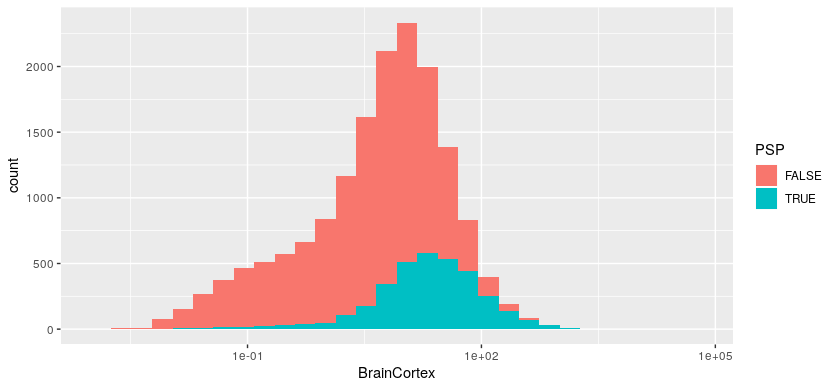
\includegraphics[width=\linewidth]{images/Rplot_corrected_gtex_histogram_log.png} 
        \caption{Histogram of expression PSP and non PSP. Log10 scale} \label{fig:gtex_histogram_log}
    \end{subfigure}
    \hfill
    \begin{subfigure}[t]{0.45\textwidth}
        \centering
        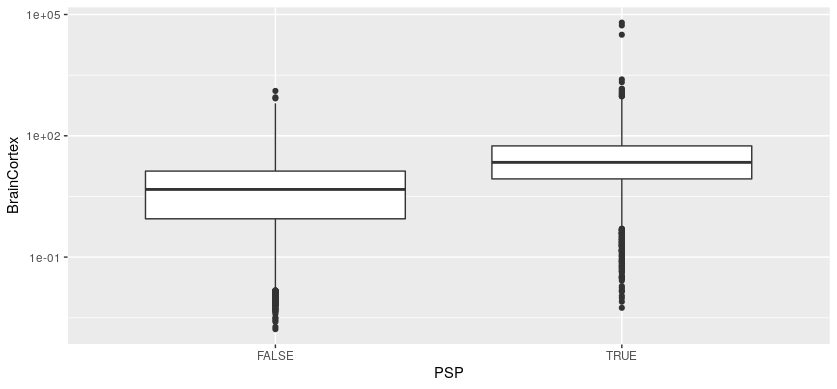
\includegraphics[width=\linewidth]{images/Rplot_corrected_gtex_boxplot_log10.png} 
        \caption{Gtex expression boxplot PSP against not PSP. Log10 scale} \label{fig:gtex_log_boxplot}
    \end{subfigure}
    \caption{Plots of gtex expression \textcolor{red}{may want to do this in subfigure packages rather than subcaption to line up edges and tidy up images in ggplot}}
    \label{fig:all_gtex_panels}
\end{figure}

\section{Genome Wide Association Studies}

To carry out inference about the association between network properties and structures and population genetic variation associated with intelligence we will need to calculate a significant test for each vertex gene. These will be calculated using MAGMA in four samples, two of intelligence and two of educational attainment.\cite{de2015magma}


\subsection{Cohorts}
\label{sec:cohorts from paper section}
%\textcolor{red}{from paper section}
Later in this thesis to investigate the efficacy of community detection in the analysis of GWA studies of cognitive ability and educational attainment I will use a discovery and replication cohort design. For consistency therefore I will refer throughout the text to the GWA study of genetic variants associated with intelligence in UK Biobank\cite{bycroft2018uk} as Intelligence\textsubscript{Discovery}  and the Phase II Educational attainment GWA study conducted using UK Biobank as Education\textsubscript{Discovery}.

We refer to the meta-analytic GWAS of intelligence carried out by Sniekers et al from the Complex Trait Genetics (CTG) lab as Intelligence\textsubscript{Replication}. \cite{sniekers2017genome}   The meta-analysis of GWA studies of educational attainment excluding UK Biobank and 23 and me by Okbay et al is referred to as Education Replication or EA2. \cite{okbay2016genome}. Details of these samples are found in the following section~\ref{sec:samples from paper section}. 

Two further samples became available after the completion of the primary analysis consisting of the largest intelligence and education cohorts to date \cite{savage2018genome}, \todo{add EA3}

\subsection{Samples}
\label{sec:samples from paper section}

Intelligence and education were the two cognitive phenotypes used to examine the effect of network structure and network communities \todo{rephrase this section}. The discovery sample for intelligence was formed using the ‘fluid’ cognitive test from UK Biobank; we shall refer to it as verbal-numerical reasoning (VNR). The VNR test contains 13 multiple choice items, six of which are verbal with the remaining seven being numerical in nature. Each individual’s VNR score was the sum of correct responses attained within a two-minute time period. This test has a large genetic correlation with intelligence scores derived from psycho-metrically validated cognitive tests. A total of 120 934 participants (mean $\chi^2$=1.52) were available for analysis who did not contribute data to the Sniekers et al data set. A full description of how data from these participants was analysed can be found in Hill et al. \cite{hill2019combined} 
UK Biobank was also used as the discovery sample for education. Summary statistics were taken from Hill et al on 273 274 participants (mean  $\chi^2$= 1.67). \cite{hill2019combined}  Education was defined as a binary choice of whether or not the individual had a University/College degree. A full description of how these data were analysed can be found in Hill et al. \cite{hill2019combined}  
To attempt to replicate any findings of enrichment for post synaptic communities, an intelligence replication dataset was formed using summary statistics obtained from the Sneikers et al. GWAS meta-analysis of intelligence (n = 78 308, mean $\chi^2$= 1.30).  \cite{sniekers2017genome}  An education replication data set was formed using summary data set from the GWAS meta-analysis by Okbay et al (n = 217 569, mean $\chi^2$= 1.43) with UK Biobank participants excluded. \cite{okbay2016genome}  (See supplemental tables 1a and 1b.)
\textcolor{red}{end from paper section}

 
\subsection{MAGMA Gene level statistics validation from other studies}

In order to ensure the accuracy of the gene level significance statistic we compared the gene level scores obtained using MAGMA to those reported in available studies.\cite{de2015magma} There were no published papers available containing a MAGMA gene-level analysis for the UK Biobank Intelligence cohort (Intelligence\textsubscript{Discovery} nor the UK Biobank Educational attainment cohort. The EA2 \cite{okbay2016genome} educational attainment paper did not report MAGMA gene scores, and in addition the Education\textsubscript{Replication} sample differs from the EA2 cohort by not including UK Biobank Educational attainment data. The only published paper reporting MAGMA gene scores from our discovery and replication cohorts of was, therefore, the Intelligence\textsubscript{Discovery} sample \cite{sniekers2017genome} (supplementary table 8 at \url{https://static-content.springer.com/esm/art\%3A10.1038\%2Fng.3869/MediaObjects/41588_2017_BFng3869_MOESM2_ESM.xlsx}).

We have, however, had access to the MTAG (Multi-trait analysis of Genome-Wide Summary data) summary data from the paper published by Hill, which contained MAGMA gene scores sheet 5 at \url{https://static-content.springer.com/esm/art\%3A10.1038\%2Fs41380-017-0001-5/MediaObjects/41380_2017_1_MOESM2_ESM.xlsx}\cite{hill2019combined}. A
can obtain a subset of the UK Biobank education data which reports MAGMA scores for Davies et al. 2016 \cite{davies2016genome} and the MAGMA results for the top 95 genes are reported in the first sheet at \todo{add SSGAC link} \url{https://static-content.springer.com/esm/art\%3A10.1038\%2Fmp.2016.45/MediaObjects/41380_2016_BFmp201645_MOESM506_ESM.xls}.\todo{ask Douglas should we store these and have a data provenance subchapter}. Finally we have recently been able to obtain summary data from the current largest GWA of intelligence by Savage et al \cite{savage2018genome} this also reports MAGMA Gene level analysis results (table S15 in supplementary materials at \url{https://www.ncbi.nlm.nih.gov/pmc/articles/PMC6411041/bin/NIHMS1006639-supplement-Supplementary_Tables.xlsx}).

\begin{table}[ht]
    \centering
    
    \begin{tabular}{llllllll}
    \toprule
        Study & n & t & df & p & Pearson & CI   \\
        \midrule
       Savage \cite{savage2018genome} & 269687 & 122.26& 352  & $<2.2 \times 10^{-16}$ & 0.99 & 0.986-0.991  \\ 
       Hill \cite{hill2019combined} & 248482 & 368.27 & 17475 & $<2.2 \times 10^{-16}$& 0.94 & 0.939-0.942 \\
       Davies (2016) \cite{davies2016genome} & 112151 & 22.08 & 93 & $<2.2 \times 10^{-16}$ & 0.92 & 0.88-0.94\\
       Sniekers \cite{sniekers2017genome}& 78308 & 466.41 & 18246 & $<2.2 \times 10^{-16}$ & 0.96 & 0.959-0.962\\
       \bottomrule
    \end{tabular}
    \caption{Correlation between MAGMA gene scores obtained from summary statistics and those published in supplementary material to papers.}
    \label{tab:Correlation between MAGMA gene scores obtained from summary statistics and those published in supplementary material to papers}
\end{table}



\subsection{Synaptic genes excluded by MAGMA}
The studies from which we obtained summary statistics (with the exception of \cite{davies2016genome} used HG19 co-ordinates and we therefore used NCBI 37.3 to provide gene boundaries in MAGMA. Using the entrez ID of the genes in the PSP for lookup the NCBI 37.3 gene boundaries supplied with MAGMA lack definitions for 17 synaptic genes. 5 additional genes are found in NCBI 38 build \footnote{code\url{source('~/RProjects/annotations_phd/R/missing_NCBI_genes.R')}}. Those genes that are found in NCBI 38 but not in 37 are shown in table~\ref{tab:Synaptic PSP genes  found in NCBI 38 but not in 37 listing included with MAGMA}.

Using NCBI Entrez Gene annotation data from \url{ftp://ftp.ncbi.nih.gov/gene/} \todo{get full url} and it was possible to identify 10 of these genes not found in NCBI 37 or 38.The annotations of the 10 synaptic genes not in NCBI 38 included with MAGMA but present in entrez gene gene info are shown in table~\ref{tab:10 synaptic genes not in NCBI 38 included with MAGMA but present in entrez gene gene info}.

A final two genes were identified using toppgene \cite{chen2009toppgene} and manual cross checking.

Two pseudo genes were not found in the standard annotation:
\begin{itemize}
    \item Entrez id:	44140, RAB1C, member RAS oncogene family pseudogene
    \item Entrez id:	440915	,POTEKP, POTE ankyrin domain family member K, pseudogene. 
\end{itemize} 



% latex table generated in R 3.6.1 by xtable 1.8-4 package
% Wed Feb 19 14:14:05 2020
% latex table generated in R 3.6.1 by xtable 1.8-4 package
% Wed Feb 19 14:15:51 2020
\begin{table}[ht]
\centering
\begin{adjustbox}{max width=\textwidth}
\begin{tabular}{rllll}
  \hline
 Gene ID & Symbol & chromosome & type of gene & Full name from nomenclature authority \\ 
  \hline
1804 & DPP6 & 7 & protein-coding & dipeptidyl peptidase like 6 \\ 
  3635 & INPP5D & 2 & protein-coding & inositol polyphosphate-5-phosphatase D \\ 
  3800 & KIF5C & 2 & protein-coding & kinesin family member 5C \\ 
  9554 & SEC22B & 1 & protein-coding & SEC22 homolog B, vesicle trafficking protein (gene/pseudogene) \\ 
  23380 & SRGAP2 & 1 & protein-coding & SLIT-ROBO Rho GTPase activating protein 2 \\ 
   \hline
\end{tabular}
\end{adjustbox}
\caption{Synaptic PSP genes  found in NCBI 38 but not in NCBI 37.3 listing included with MAGMA}
\label{tab:Synaptic PSP genes  found in NCBI 38 but not in 37 listing included with MAGMA}
\end{table}
   


\begin{table}[ht]
\centering
\begin{adjustbox}{max width=\textwidth}
\begin{tabular}{rllll}
  \hline
 Gene ID & Symbol & chromosome & type of gene & Full name from nomenclature authority \\ 
  \hline
293 & SLC25A6 & X$|$Y & protein-coding & solute carrier family 25 member 6 \\ 
  3493 & IGHA1 & 14 & other & immunoglobulin heavy constant alpha 1 \\ 
  3500 & IGHG1 & 14 & other & immunoglobulin heavy constant gamma 1 (G1m marker) \\ 
  3502 & IGHG3 & 14 & other & immunoglobulin heavy constant gamma 3 (G3m marker) \\ 
  3503 & IGHG4 & 14 & other & immunoglobulin heavy constant gamma 4 (G4m marker) \\ 
  3507 & IGHM & 14 & other & immunoglobulin heavy constant mu \\ 
  3514 & IGKC & 2 & other & immunoglobulin kappa constant \\ 
  4509 & ATP8 & MT & protein-coding & mitochondrially encoded ATP synthase 8 \\ 
  4513 & COX2 & MT & protein-coding & mitochondrially encoded cytochrome c oxidase II \\ 
  4538 & ND4 & MT & protein-coding & mitochondrially encoded NADH dehydrogenase 4 \\ 
   \hline
\end{tabular}
\end{adjustbox}
\caption{10 synaptic genes not in NCBI 38 included with MAGMA but present in entrez gene gene info}
\label{tab:10 synaptic genes not in NCBI 38 included with MAGMA but present in entrez gene gene info}
\end{table}


\textcolor{red}{Move some methods here from introduction}


\subsection{Intelligence Replication GWGWAS}


\subsubsection{Methods}
The Intelligence\textsubscript{Replication} sample was made using the data are from the 2017 ``intelligence wave 1" study by Sniekers et al. \cite{sniekers2017genome}. 
GWAS Summary data was downloaded from the authors department, the Complex Trait Genomics (CTG) lab\footnote{ \url{https://ctg.cncr.nl/documents/p1651/sumstats.txt.gz}}. This study is a meta-analysis of 78,308 individuals. The individuals came from 13 cohorts and 29,610 were reported for the first time. The individuals in this study meta-analysis do not overlap with any of the other studies used in this thesis as those individuals derived from UK Biobank were excluded from the Intelligence\textsubscript{Discovery} sample summary statistics prepared by Dr Hill. The authors report the results of a Genome Wide Gene Association (GWGWAS) analysis using MAGMA finding 47 genome wide significant genes.\cite{sniekers2017genome},\cite{de2015magma}

Gene level scores were calculated using MAGMA GWAS using NCBI 37.3 to delineate gene boundaries (MAGMA version 1.06). No window was used around gene boundaries \footnote{Code to produce the following tables is at \url{source('~/RProjects/paper_xls_output/R/0_write_MAGMA_gene_level_results_PhD.R')} }.
 The number of individuals in individal  SNPs were tested was available as part of the summary data and this information was included in the command line argument to MAGMA. SNPs tested in less than 50 individuals were excluded. The command line arguments given to MAGMA for this and all analyses are found at github\todo{add github}.
\subsubsection{Results}
18262 genes were assigned gene level p values using MAGMA v1.06.
The Bonferroni correction for multiple comparisons was used to calculate a genome wide significance level ($\alpha$ = 0.05/18262; p=$2.74 \times 10^{-06}$),  47 significant genes were identified using MAGMA and summary statistics as was the case in the original paper \cite{sniekers2017genome}. 16 of these were found in the PSP (34.0\%) as shown in table~\ref{tab:significant genes}.
\todo{ORA ie psp vs genome}
\todo{The table wrappings around longtable are to keep the word count correct once we have final word count 8I will remove them and move the caption to just below begin longtable}

All significant genes are shown in table \ref{tab:Significant genes in ctg MAGMA GWAS}, significant synaptic genes are shown in table \ref{tab:Significant genes in ctg MAGMA GWAS}

\begin{table}[ht]
    \centering
    \begin{tabular}{cccc}
    \toprule
         Study & n significant genes & n synaptic significant genes & percent (\%) in PSP \\
      \midrule  
         Intelligence\textsubscript{Replication}\cite{sniekers2017genome} & 16 & 47 & 34.0 \\
         Education\textsubscript{Replication}\cite{okbay2016genome} & 25 & 99 & 25.2 \\
         Intelligence\textsubscript{Discovery}\cite{hill2019combined} & 51 & 196 & 26.0\\
         Education\textsubscript{Discovery}\cite{hill2019combined} & 58 & 235 & 24.7\\
         \bottomrule
    \end{tabular}
    \caption{Number of genome wide significant genes found in each sample using MAGMA Genome Wide Gene Association Analysis Study  (GWGWAS)}
    \label{tab:significant genes}
\end{table}
% latex table generated in R 3.6.2 by xtable 1.8-4 package
% Thu Jan  2 13:21:27 2020

% latex table generated in R 3.6.1 by xtable 1.8-4 package
% Wed Feb 19 11:25:28 2020
\begin{table}[ht]
\centering
\begin{tabular}{rlrrrr}
  \hline
 Gene ID & Symbol & Chromosome & N SNP & Z statistic & P \\ 
  \hline
1434 & CSE1L &  20 & 176 & 5.96 & $1.26 \times 10^{-9}$ \\ 
  60412 & EXOC4 &   7 & 2184 & 5.88 & $1.99 \times 10^{-9}$ \\ 
  55964 & SEPT3 &  22 &  69 & 5.75 & $4.35 \times 10^{-9}$ \\ 
  6138 & RPL15 &   3 &  19 & 5.40 & $3.35 \times 10^{-8}$ \\ 
  23109 & DDN &  12 &   8 & 5.35 & $4.41 \times 10^{-8}$ \\ 
  85358 & SHANK3 &  22 & 199 & 5.31 & $5.49 \times 10^{-8}$ \\ 
  487 & ATP2A1 &  16 &  47 & 5.23 & $8.37 \times 10^{-8}$ \\ 
  11273 & ATXN2L &  16 &  36 & 5.17 & $1.17 \times 10^{-7}$ \\ 
  2870 & GRK6 &   5 &  39 & 5.07 & $2.03 \times 10^{-7}$ \\ 
  28512 & NKIRAS1 &   3 &  73 & 5.04 & $2.29 \times 10^{-7}$ \\ 
  4700 & NDUFA6 &  22 &  16 & 5.04 & $2.32 \times 10^{-7}$ \\ 
  4733 & DRG1 &  22 &  99 & 4.83 & $6.91 \times 10^{-7}$ \\ 
  10564 & ARFGEF2 &  20 & 406 & 4.80 & $7.83 \times 10^{-7}$ \\ 
  7284 & TUFM &  16 &   7 & 4.79 & $8.49 \times 10^{-7}$ \\ 
  553115 & PEF1 &   1 &  30 & 4.77 & $9.17 \times 10^{-7}$ \\ 
  8411 & EEA1 &  12 & 475 & 4.61 & $2.03 \times 10^{-6}$ \\ 
   \hline
\end{tabular}
\caption{PSP synaptic genes meeting genome wide significant in Intelligence Discovery study. 16 genes, alpha bonferroni $2.74 \times 10^{-06}$. N SNP = number of SNPs found within gene boundaries in study.  } 
\label{tab:Significant synaptic genes in ctg MAGMA GWAS2}
\end{table}

\subsection{Education replication}

\subsubsection{Methods}
The summary statistics for Education\textsubscript{Replication} are generated using individuals taken from the EA2 (Educational Attainment 2) meta-analytic GWA study of educational attainment.\cite{okbay2016genome}\todo{educational attainment was defined as}.  The published study is of 293,723 individuals with 111,349 independent samples from UK Biobank. A combined meta-analysis was also made of the discovery and replication cohorts (n=405702). This allowed an increase in the number of genome wide loci reported from 74 to 162. Due to Institutional Review Board (IRB) restrictions which do not allow reporting of over 10,000 SNPs the results provided on the website are of n=328917 individuals excluding 76155 individuals from 23andme. The summary statistics that were made available to us by the authors were therefore of the sample without 23 and me and excluding UK Biobank n= 217568 (293723 - 76155 = 217568). \cite{okbay2016genome} supplemental information \url{http://ssgac.org/documents/SI_74_loci_educational_attainment.pdf} p 16. The summary statistics used were those unsorted by sex. 

EA2 data can be downloaded from \url{https://www.thessgac.org/data}. The modified summary statistics excluding UK Biobank and 23andMe  are deposited with \textcolor{red}{DATASTORE}.

\subsubsection{Results}

17942 genes were assigned a significance score using MAGMA 1.06 based on the SNP's present in the summary statistics.The Bonferroni correction for multiple comparisons was used to calculate a genome wide significance level ($\alpha$ = 0.05/17942; p=$2.79 \times 10^{-06}$). With this $\alpha$ level 99 genes were identified of genome wide significance. 25 (25.3\%) of these were found in the synaptic PSP (see table~\ref{tab:significant genes}).

Genome wide significant genes  are shown in table \ref{tab:Significant genes in EA2 MAGMA GWAS}, significant synaptic genes are shown in table \ref{tab:Significant synaptic genes in EA2  MAGMA GWAS}

% latex table generated in R 3.6.2 by xtable 1.8-4 package
% Thu Jan  2 13:31:54 2020

% latex table generated in R 3.6.1 by xtable 1.8-4 package
% Wed Feb 19 15:25:56 2020
\begin{table}[ht]
\centering
\begin{tabular}{rllrrr}
  \hline
GENE & SYMBOL & CHR & NSNPS & ZSTAT & P \\ 
  \hline
79012 & CAMKV & 3 &  17 & 7.16 & $3.95 \times 10^{-13}$ \\ 
  8927 & BSN & 3 & 148 & 6.98 & $1.45 \times 10^{-12}$ \\ 
  327 & APEH & 3 &   8 & 6.44 & $5.86 \times 10^{-11}$ \\ 
  387 & RHOA & 3 &  90 & 6.38 & $8.67 \times 10^{-11}$ \\ 
  2876 & GPX1 & 3 &   2 & 6.25 & $2.01 \times 10^{-10}$ \\ 
  57605 & PITPNM2 & 12 & 167 & 6.06 & $6.94 \times 10^{-10}$ \\ 
  10419 & PRMT5 & 14 &  16 & 5.77 & $4.07 \times 10^{-9}$ \\ 
  5792 & PTPRF & 1 & 260 & 5.67 & $7.09 \times 10^{-9}$ \\ 
  5662 & PSD & 10 &  23 & 5.67 & $7.20 \times 10^{-9}$ \\ 
  55729 & ATF7IP & 12 & 374 & 5.60 & $1.08 \times 10^{-8}$ \\ 
  30819 & KCNIP2 & 10 &  28 & 5.57 & $1.28 \times 10^{-8}$ \\ 
  4208 & MEF2C & 5 & 339 & 5.44 & $2.63 \times 10^{-8}$ \\ 
  257194 & NEGR1 & 1 & 1898 & 5.40 & $3.34 \times 10^{-8}$ \\ 
  26575 & RGS17 & 6 & 411 & 5.35 & $4.31 \times 10^{-8}$ \\ 
  29919 & C18orf8 & 18 &  53 & 5.33 & $4.85 \times 10^{-8}$ \\ 
  2823 & GPM6A & 4 & 1150 & 5.31 & $5.35 \times 10^{-8}$ \\ 
  5144 & PDE4D & 5 & 3995 & 5.06 & $2.14 \times 10^{-7}$ \\ 
  10724 & MGEA5 & 10 &  48 & 5.04 & $2.28 \times 10^{-7}$ \\ 
  4744 & NEFH & 22 &  31 & 4.81 & $7.47 \times 10^{-7}$ \\ 
  60412 & EXOC4 & 7 & 1394 & 4.69 & $1.37 \times 10^{-6}$ \\ 
  4137 & MAPT & 17 & 696 & 4.68 & $1.47 \times 10^{-6}$ \\ 
  5869 & RAB5B & 12 &  44 & 4.66 & $1.55 \times 10^{-6}$ \\ 
  9859 & CEP170 & 1 & 160 & 4.63 & $1.82 \times 10^{-6}$ \\ 
  4905 & NSF & 17 &  66 & 4.61 & $1.99 \times 10^{-6}$ \\ 
  11122 & PTPRT & 20 & 3517 & 4.58 & $2.28 \times 10^{-6}$ \\ 
   \hline
\end{tabular}
\caption{Significant synaptic genes in EA2  MAGMA GWAS} 
\label{tab:Significant synaptic genes in EA2  MAGMA GWAS}
\end{table}




\subsection{Intelligence Discovery Phase II}



\subsubsection{Methods}
The GWAS summary statistics for the Intelligence\textsubscript{Discovery} Phase II are taken from UK Biobank Phase II. The data were obtained from the CCACE \todo{full title} from the author Dr D.W Hill  . The sample size is n=120 934. For further details on the cohorts see \cite{hill2019combined}.


\subsubsection{Results}
With an alpha bonferroni level of  $2.73\times 10^{-06}$, 196 genome wide significant genes were found at GWGWAS using MAGMA. Of these 51 genes were in the PSP synaptic set (26.0\% of total) see table~\ref{tab:significant genes}

Significant genes at alpha bonferroni level are shown in table \ref{tab:Significant synaptic genes in UKBB int  MAGMA GWAS}, significant synaptic genes are shown in table \ref{tab:Significant genes in UKBB int MAGMA GWAS}



% latex table generated in R 3.6.1 by xtable 1.8-4 package
% Fri Feb 21 11:27:26 2020
\begin{table}[ht]
\centering
\begin{tabular}{rllrrr}
  \hline
GENE & SYMBOL & CHR & NSNPS & ZSTAT & P \\ 
  \hline
8341 & HIST1H2BN & 6 &  67 & 7.57 & $1.85 \times 10^{-14}$ \\ 
  1434 & CSE1L & 20 & 195 & 7.10 & $6.36 \times 10^{-13}$ \\ 
  4208 & MEF2C & 5 & 603 & 7.04 & $9.75 \times 10^{-13}$ \\ 
  8927 & BSN & 3 & 312 & 7.00 & $1.29 \times 10^{-12}$ \\ 
  257194 & NEGR1 & 1 & 3314 & 6.89 & $2.73 \times 10^{-12}$ \\ 
  487 & ATP2A1 & 16 &  94 & 6.86 & $3.56 \times 10^{-12}$ \\ 
  27044 & SND1 & 7 & 1381 & 6.81 & $5.01 \times 10^{-12}$ \\ 
  11273 & ATXN2L & 16 &  60 & 6.78 & $5.95 \times 10^{-12}$ \\ 
  8085 & KMT2D & 12 &  96 & 6.78 & $6.20 \times 10^{-12}$ \\ 
  79012 & CAMKV & 3 &  30 & 6.74 & $7.94 \times 10^{-12}$ \\ 
  10564 & ARFGEF2 & 20 & 440 & 6.47 & $4.84 \times 10^{-11}$ \\ 
  23109 & DDN & 12 &  11 & 6.43 & $6.38 \times 10^{-11}$ \\ 
  28512 & NKIRAS1 & 3 & 104 & 6.28 & $1.71 \times 10^{-10}$ \\ 
  6138 & RPL15 & 3 &  36 & 6.20 & $2.90 \times 10^{-10}$ \\ 
  7284 & TUFM & 16 &  11 & 6.14 & $4.18 \times 10^{-10}$ \\ 
  553115 & PEF1 & 1 &  41 & 6.08 & $6.09 \times 10^{-10}$ \\ 
  387 & RHOA & 3 & 186 & 6.07 & $6.33 \times 10^{-10}$ \\ 
  64943 & NT5DC2 & 3 &  58 & 5.93 & $1.51 \times 10^{-9}$ \\ 
  327 & APEH & 3 &  18 & 5.91 & $1.71 \times 10^{-9}$ \\ 
  575 & ADGRB1 & 8 & 404 & 5.91 & $1.74 \times 10^{-9}$ \\ 
  30819 & KCNIP2 & 10 &  51 & 5.78 & $3.76 \times 10^{-9}$ \\ 
  8340 & HIST1H2BL & 6 &   2 & 5.52 & $1.69 \times 10^{-8}$ \\ 
  2903 & GRIN2A & 16 & 2864 & 5.52 & $1.70 \times 10^{-8}$ \\ 
  7840 & ALMS1 & 2 & 921 & 5.47 & $2.27 \times 10^{-8}$ \\ 
  3009 & HIST1H1B & 6 &  14 & 5.40 & $3.31 \times 10^{-8}$ \\ 
  2774 & GNAL & 18 & 1131 & 5.34 & $4.53 \times 10^{-8}$ \\ 
  11122 & PTPRT & 20 & 5717 & 5.33 & $4.78 \times 10^{-8}$ \\ 
  8895 & CPNE3 & 8 & 231 & 5.30 & $5.73 \times 10^{-8}$ \\ 
  1499 & CTNNB1 & 3 & 143 & 5.27 & $7.00 \times 10^{-8}$ \\ 
  2876 & GPX1 & 3 &   5 & 5.25 & $7.79 \times 10^{-8}$ \\ 
  3992 & FADS1 & 11 &  38 & 5.21 & $9.23 \times 10^{-8}$ \\ 
  60412 & EXOC4 & 7 & 3112 & 5.21 & $9.24 \times 10^{-8}$ \\ 
  23312 & DMXL2 & 15 & 642 & 5.15 & $1.31 \times 10^{-7}$ \\ 
  8359 & HIST1H4A & 6 &   2 & 5.05 & $2.26 \times 10^{-7}$ \\ 
  777 & CACNA1E & 1 & 1484 & 4.99 & $3.09 \times 10^{-7}$ \\ 
  5702 & PSMC3 & 11 &  35 & 4.95 & $3.80 \times 10^{-7}$ \\ 
  7486 & WRN & 8 & 551 & 4.94 & $3.97 \times 10^{-7}$ \\ 
  23196 & FAM120A & 9 & 543 & 4.92 & $4.23 \times 10^{-7}$ \\ 
  23301 & EHBP1 & 2 & 934 & 4.91 & $4.56 \times 10^{-7}$ \\ 
  203068 & TUBB & 6 &  30 & 4.83 & $6.96 \times 10^{-7}$ \\ 
  10724 & MGEA5 & 10 &  98 & 4.82 & $7.32 \times 10^{-7}$ \\ 
  6272 & SORT1 & 1 & 272 & 4.75 & $9.94 \times 10^{-7}$ \\ 
  150726 & FBXO41 & 2 &  54 & 4.75 & $1.03 \times 10^{-6}$ \\ 
  3760 & KCNJ3 & 2 & 777 & 4.73 & $1.12 \times 10^{-6}$ \\ 
  5686 & PSMA5 & 1 &  95 & 4.68 & $1.40 \times 10^{-6}$ \\ 
  10919 & EHMT2 & 6 &  82 & 4.64 & $1.72 \times 10^{-6}$ \\ 
  2893 & GRIA4 & 11 & 1378 & 4.61 & $1.97 \times 10^{-6}$ \\ 
  27072 & VPS41 & 7 & 913 & 4.60 & $2.08 \times 10^{-6}$ \\ 
  5898 & RALA & 7 & 288 & 4.58 & $2.37 \times 10^{-6}$ \\ 
  4857 & NOVA1 & 14 & 609 & 4.56 & $2.51 \times 10^{-6}$ \\ 
  55604 & LRRC16A & 6 & 2282 & 4.55 & $2.64 \times 10^{-6}$ \\ 
   \hline
\end{tabular}
\caption{Significant synaptic genes in UKBB int  MAGMA GWAS} 
\label{tab:Significant synaptic genes in UKBB int  MAGMA GWAS}
\end{table}







\section{UKBB Education Discovery}

\subsubsection{Methods}
The GWAS summary statistics for the Education\textsubscript{Discovery} Phase II are taken from UK Biobank Phase II. The data were obtained from the CCACE \todo{full title} from the authors Dr D.W Hill and Dr G. Davies. The sample size is n=273 274.

\subsubsection{Results}
At an bonferroni adjusted alpha level of $2.73 \times 10^{-06}$, 235 significant genes were identified. Of these 58 were members of the PSP (24.7\%).  

Significant genes at alpha bonferroni level are shown in table \ref{tab:Significant genes in UKBB edu MAGMA GWAS}, significant synaptic genes are shown in table \ref{tab:Significant synaptic genes in UKBB edu  MAGMA GWAS}

% latex table generated in R 3.6.1 by xtable 1.8-4 package
% Fri Feb 21 12:10:53 2020
% latex table generated in R 3.6.2 by xtable 1.8-4 package
% Thu Jan  2 13:49:56 2020

\begin{table}[ht]
\centering
\begin{tabular}{rllrrr}
  \hline
GENE & SYMBOL & CHR & NSNPS & ZSTAT & P \\ 
  \hline
8927 & BSN & 3 & 312 & 10.79 & $2.02 \times 10^{-27}$ \\ 
  79012 & CAMKV & 3 &  30 & 10.03 & $5.67 \times 10^{-24}$ \\ 
  387 & RHOA & 3 & 186 & 9.10 & $4.37 \times 10^{-20}$ \\ 
  327 & APEH & 3 &  18 & 8.93 & $2.05 \times 10^{-19}$ \\ 
  2876 & GPX1 & 3 &   5 & 7.49 & $3.40 \times 10^{-14}$ \\ 
  10659 & CELF2 & 10 & 2900 & 7.49 & $3.57 \times 10^{-14}$ \\ 
  1951 & CELSR3 & 3 &  51 & 7.04 & $9.56 \times 10^{-13}$ \\ 
  4905 & NSF & 17 & 146 & 7.04 & $9.70 \times 10^{-13}$ \\ 
  51517 & NCKIPSD & 3 &  64 & 6.98 & $1.45 \times 10^{-12}$ \\ 
  5144 & PDE4D & 5 & 6306 & 6.94 & $1.96 \times 10^{-12}$ \\ 
  257194 & NEGR1 & 1 & 3314 & 6.70 & $1.06 \times 10^{-11}$ \\ 
  5792 & PTPRF & 1 & 473 & 6.69 & $1.13 \times 10^{-11}$ \\ 
  4137 & MAPT & 17 & 891 & 6.62 & $1.84 \times 10^{-11}$ \\ 
  30819 & KCNIP2 & 10 &  51 & 6.39 & $8.50 \times 10^{-11}$ \\ 
  9842 & PLEKHM1 & 17 & 177 & 6.34 & $1.14 \times 10^{-10}$ \\ 
  8898 & MTMR2 & 11 & 373 & 6.31 & $1.38 \times 10^{-10}$ \\ 
  343099 & CCDC18 & 1 & 421 & 6.28 & $1.69 \times 10^{-10}$ \\ 
  3831 & KLC1 & 14 & 310 & 6.23 & $2.40 \times 10^{-10}$ \\ 
  10724 & MGEA5 & 10 &  98 & 6.00 & $9.88 \times 10^{-10}$ \\ 
  11273 & ATXN2L & 16 &  60 & 5.94 & $1.39 \times 10^{-9}$ \\ 
  5576 & PRKAR2A & 3 & 212 & 5.79 & $3.58 \times 10^{-9}$ \\ 
  487 & ATP2A1 & 16 &  94 & 5.78 & $3.81 \times 10^{-9}$ \\ 
  8428 & STK24 & 13 & 656 & 5.75 & $4.46 \times 10^{-9}$ \\ 
  4208 & MEF2C & 5 & 603 & 5.69 & $6.25 \times 10^{-9}$ \\ 
  4134 & MAP4 & 3 & 578 & 5.56 & $1.36 \times 10^{-8}$ \\ 
  5095 & PCCA & 13 & 1504 & 5.50 & $1.85 \times 10^{-8}$ \\ 
  7284 & TUFM & 16 &  11 & 5.46 & $2.34 \times 10^{-8}$ \\ 
  23031 & MAST3 & 19 & 273 & 5.43 & $2.82 \times 10^{-8}$ \\ 
  23671 & TMEFF2 & 2 & 1282 & 5.42 & $3.01 \times 10^{-8}$ \\ 
  8085 & KMT2D & 12 &  96 & 5.36 & $4.09 \times 10^{-8}$ \\ 
  23334 & SZT2 & 1 & 201 & 5.36 & $4.25 \times 10^{-8}$ \\ 
  3781 & KCNN2 & 5 & 586 & 5.25 & $7.70 \times 10^{-8}$ \\ 
  56853 & CELF4 & 18 & 1442 & 5.24 & $7.84 \times 10^{-8}$ \\ 
  5662 & PSD & 10 &  45 & 5.20 & $1.01 \times 10^{-7}$ \\ 
  221935 & SDK1 & 7 & 7054 & 5.14 & $1.34 \times 10^{-7}$ \\ 
  60412 & EXOC4 & 7 & 3112 & 5.08 & $1.92 \times 10^{-7}$ \\ 
  5859 & QARS & 3 &  19 & 5.08 & $1.93 \times 10^{-7}$ \\ 
  4857 & NOVA1 & 14 & 609 & 5.07 & $1.95 \times 10^{-7}$ \\ 
  118 & ADD1 & 4 & 403 & 5.06 & $2.14 \times 10^{-7}$ \\ 
  10419 & PRMT5 & 14 &  26 & 5.01 & $2.76 \times 10^{-7}$ \\ 
  7248 & TSC1 & 9 & 204 & 4.95 & $3.74 \times 10^{-7}$ \\ 
  29919 & C18orf8 & 18 & 117 & 4.92 & $4.43 \times 10^{-7}$ \\ 
  25791 & NGEF & 2 & 794 & 4.91 & $4.60 \times 10^{-7}$ \\ 
  27132 & CPNE7 & 16 & 145 & 4.84 & $6.59 \times 10^{-7}$ \\ 
  23109 & DDN & 12 &  11 & 4.75 & $9.92 \times 10^{-7}$ \\ 
  51337 & THEM6 & 8 &  42 & 4.72 & $1.16 \times 10^{-6}$ \\ 
  1152 & CKB & 14 &   9 & 4.71 & $1.22 \times 10^{-6}$ \\ 
  5686 & PSMA5 & 1 &  95 & 4.65 & $1.63 \times 10^{-6}$ \\ 
  6272 & SORT1 & 1 & 272 & 4.65 & $1.65 \times 10^{-6}$ \\ 
  788 & SLC25A20 & 3 & 104 & 4.64 & $1.76 \times 10^{-6}$ \\ 
  3799 & KIF5B & 10 & 152 & 4.63 & $1.82 \times 10^{-6}$ \\ 
  2870 & GRK6 & 5 &  52 & 4.62 & $1.89 \times 10^{-6}$ \\ 
  9378 & NRXN1 & 2 & 6004 & 4.61 & $2.01 \times 10^{-6}$ \\ 
  22907 & DHX30 & 3 & 103 & 4.57 & $2.44 \times 10^{-6}$ \\ 
  120 & ADD3 & 10 & 613 & 4.57 & $2.44 \times 10^{-6}$ \\ 
  575 & ADGRB1 & 8 & 404 & 4.57 & $2.48 \times 10^{-6}$ \\ 
  1993 & ELAVL2 & 9 & 729 & 4.56 & $2.55 \times 10^{-6}$ \\ 
  9529 & BAG5 & 14 &  17 & 4.55 & $2.72 \times 10^{-6}$ \\ 
   \hline
\end{tabular}
\caption{Significant synaptic genes in UKBB edu  MAGMA GWAS} 
\label{tab:Significant synaptic genes in UKBB edu  MAGMA GWAS}
\end{table}




\subsection{preamble}
No further analysis may be necessary and it may be possible to carry out gene ontology analysis for our gene results. We will not report GSA in MAGMA for an unsorted gene set list except where it has not been done by previous authors but we might ask if there are common features to the significant genes found in MAGMA Gene level analysis of the GWA summary data.

\subsection{Education - Discovery}

\subsubsection{Biological process}\todo{Gene ontology over those not in PSP}
    See table~\ref{tab:GO analysis ukbbed_bp_all_sig_genome.txt} for significant genes against entire genome. 
    No significant on GO slim against entire genome all significant
No significant biological pathway with the entire synapse as background (Fishers exact test, FDR rate for multiple comparisons - Panther)
\subsubsection{Biological process all genes genome as background}
See table~\ref{tab:GO analysis ukbbed_bp_all_sig_genome.txt}
% latex table generated in R 3.6.2 by xtable 1.8-4 package
% Mon Mar  2 16:15:50 2020
\begin{table}[ht]
\centering
\begin{adjustbox}{width=\textwidth}
\begin{tabular}{lrrrlrrr}
  \hline
GO biological process complete & Homo sapiens ref & Test genes & Expected & Over/under & Fold enrichment & p value & FDR \\ 
  \hline
neuron development (GO:0048666) & 824 & 29 & 8 & + & 3.7 & $2.29 \times 10^{-9}$ & 0.00004 \\ 
  cellular process (GO:0009987) & 14616 & 175 & 139 & + & 1.2 & $4.65 \times 10^{-9}$ & 0.00004 \\ 
  neuron differentiation (GO:0030182) & 1018 & 29 & 10 & + & 3.0 & $1.98 \times 10^{-7}$ & 0.00105 \\ 
  cellular component organization (GO:0016043) & 5620 & 88 & 54 & + & 1.6 & $2.09 \times 10^{-7}$ & 0.00083 \\ 
  neuron projection development (GO:0031175) & 679 & 23 & 6 & + & 3.5 & $2.32 \times 10^{-7}$ & 0.00074 \\ 
  neurogenesis (GO:0022008) & 1664 & 39 & 16 & + & 2.5 & $2.35 \times 10^{-7}$ & 0.00062 \\ 
  cell development (GO:0048468) & 1623 & 38 & 15 & + & 2.5 & $3.58 \times 10^{-7}$ & 0.00082 \\ 
  cellular component organization or biogenesis (GO:0071840) & 5810 & 89 & 55 & + & 1.6 & $4.47 \times 10^{-7}$ & 0.00089 \\ 
  generation of neurons (GO:0048699) & 1562 & 37 & 15 & + & 2.5 & $4.57 \times 10^{-7}$ & 0.00081 \\ 
  nervous system development (GO:0007399) & 2373 & 48 & 23 & + & 2.1 & $5.00 \times 10^{-7}$ & 0.00080 \\ 
  multicellular organismal process (GO:0032501) & 7014 & 100 & 67 & + & 1.5 & $1.70 \times 10^{-6}$ & 0.00246 \\ 
  cell morphogenesis (GO:0000902) & 721 & 22 & 7 & + & 3.2 & $2.31 \times 10^{-6}$ & 0.00306 \\ 
  regulation of multicellular organismal process (GO:0051239) & 3183 & 56 & 30 & + & 1.8 & $4.03 \times 10^{-6}$ & 0.00493 \\ 
  cellular component morphogenesis (GO:0032989) & 825 & 23 & 8 & + & 2.9 & $5.75 \times 10^{-6}$ & 0.00655 \\ 
  biological\_process (GO:0008150) & 17780 & 190 & 170 & + & 1.1 & $6.95 \times 10^{-6}$ & 0.00692 \\ 
  Unclassified (UNCLASSIFIED) & 3071 & 9 & 29 & - & 0.3 & $6.95 \times 10^{-6}$ & 0.00738 \\ 
  neuron projection morphogenesis (GO:0048812) & 490 & 17 & 5 & + & 3.6 & $7.02 \times 10^{-6}$ & 0.00658 \\ 
  plasma membrane bounded cell projection morphogenesis (GO:0120039) & 494 & 17 & 5 & + & 3.6 & $7.78 \times 10^{-6}$ & 0.00688 \\ 
  cell morphogenesis involved in neuron differentiation (GO:0048667) & 442 & 16 & 4 & + & 3.8 & $7.92 \times 10^{-6}$ & 0.00664 \\ 
  cell projection morphogenesis (GO:0048858) & 498 & 17 & 5 & + & 3.6 & $8.61 \times 10^{-6}$ & 0.00686 \\ 
  regulation of biological quality (GO:0065008) & 4106 & 66 & 39 & + & 1.7 & $9.38 \times 10^{-6}$ & 0.00712 \\ 
  cell morphogenesis involved in differentiation (GO:0000904) & 562 & 18 & 5 & + & 3.4 & $1.07 \times 10^{-5}$ & 0.00778 \\ 
  axon development (GO:0061564) & 412 & 15 & 4 & + & 3.8 & $1.44 \times 10^{-5}$ & 0.00996 \\ 
  cell part morphogenesis (GO:0032990) & 520 & 17 & 5 & + & 3.4 & $1.48 \times 10^{-5}$ & 0.00981 \\ 
  regulation of cellular component organization (GO:0051128) & 2529 & 46 & 24 & + & 1.9 & $1.68 \times 10^{-5}$ & 0.01070 \\ 
  biological regulation (GO:0065007) & 12470 & 148 & 119 & + & 1.2 & $2.21 \times 10^{-5}$ & 0.01350 \\ 
  cell projection organization (GO:0030030) & 1159 & 27 & 11 & + & 2.4 & $2.99 \times 10^{-5}$ & 0.01760 \\ 
  movement of cell or subcellular component (GO:0006928) & 1544 & 32 & 15 & + & 2.2 & $3.55 \times 10^{-5}$ & 0.02020 \\ 
  regulation of biological process (GO:0050789) & 11770 & 141 & 112 & + & 1.3 & $3.80 \times 10^{-5}$ & 0.02090 \\ 
  plasma membrane bounded cell projection organization (GO:0120036) & 1114 & 26 & 11 & + & 2.5 & $4.36 \times 10^{-5}$ & 0.02310 \\ 
  multi-organism process (GO:0051704) & 2842 & 48 & 27 & + & 1.8 & $7.08 \times 10^{-5}$ & 0.03640 \\ 
  regulation of system process (GO:0044057) & 594 & 17 & 6 & + & 3.0 & $7.43 \times 10^{-5}$ & 0.03700 \\ 
  axonogenesis (GO:0007409) & 378 & 13 & 4 & + & 3.6 & $9.44 \times 10^{-5}$ & 0.04560 \\ 
  developmental process (GO:0032502) & 5901 & 82 & 56 & + & 1.5 & $1.01 \times 10^{-4}$ & 0.04730 \\ 
   \hline
\end{tabular}
\end{adjustbox}
\caption{GO analysis ukbbed bp all sig genome.txt} 
\label{tab:GO analysis ukbbed_bp_all_sig_genome.txt}

\end{table}


\subsubsection{Biological process significant synaptic against PSP}
Nil significant
\subsubsection{Molecular function}
No significant biological pathway with the entire synapse as background (Fishers exact test, FDR rate for multiple comparisons - Panther)

No significant for MF entire synapse all significant GO slim

Complete GO (NOT SLIM) MF all significant synaspe only three not unclassified top protein binding FDR 0.005 table~\ref{tab:GO analysis ukbbed mf all sig genome.txt}




% latex table generated in R 3.6.2 by xtable 1.8-4 package
% Mon Mar  2 16:33:04 2020
\begin{table}[ht]
\centering
\begin{adjustbox}{width=\textwidth}
\begin{tabular}{lrrrlrrr}
  \hline
GO molecular function complete & Homo sapiens ref & Test genes & Expected & Over/under & Fold enrichment & p value & FDR \\ 
  \hline
protein binding (GO:0005515) & 12112 & 149 & 116 & + & 1.3 & $1.06 \times 10^{-6}$ & 0.00500 \\ 
  binding (GO:0005488) & 15292 & 173 & 146 & + & 1.2 & $5.14 \times 10^{-6}$ & 0.01210 \\ 
  molecular\_function (GO:0003674) & 17659 & 188 & 169 & + & 1.1 & $3.81 \times 10^{-5}$ & 0.05980 \\ 
  Unclassified (UNCLASSIFIED) & 3192 & 11 & 30 & - & 0.4 & $3.81 \times 10^{-5}$ & 0.04490 \\ 
   \hline
\end{tabular}
\end{adjustbox}
\caption{GO analysis ukbbed mf all sig genome.txt} 
\label{tab:GO analysis ukbbed mf all sig genome.txt}
\end{table}

\subsubsection{Molecular Function all synaptic against synaptic background}
No significant

\subsubsection{Cellular Component}
No significant biological pathway with the entire synapse as background (Fishers exact test, FDR rate for multiple comparisons - Panther)

No significant for CC entire synapse all significant GO slim

For all significant genes CC see table~\ref{tab:GO analysis ukbbed cc all sig genome.txt}
% latex table generated in R 3.6.2 by xtable 1.8-4 package
% Mon Mar  2 16:38:29 2020
\begin{table}[ht]
\centering
\begin{adjustbox}{width=\textwidth}
\begin{tabular}{lrrrlrrr}
  \hline
GO cellular component complete & Homo sapiens ref & Test genes & Expected & Over/under & Fold enrichment & p value & FDR \\ 
  \hline
intracellular (GO:0005622) & 14473 & 172 & 138 & + & 1.2 & $3.92 \times 10^{-8}$ & 0.00008 \\ 
  cytosol (GO:0005829) & 5199 & 83 & 50 & + & 1.7 & $2.55 \times 10^{-7}$ & 0.00026 \\ 
  cellular\  component (GO:0005575) & 18818 & 197 & 180 & + & 1.1 & $7.35 \times 10^{-7}$ & 0.00037 \\ 
  Unclassified (UNCLASSIFIED) & 2033 & 2 & 19 & - & 0.1 & $7.35 \times 10^{-7}$ & 0.00049 \\ 
  organelle (GO:0043226) & 13710 & 161 & 131 & + & 1.2 & $3.75 \times 10^{-6}$ & 0.00151 \\ 
  postsynapse (GO:0098794) & 644 & 20 & 6 & + & 3.2 & $5.31 \times 10^{-6}$ & 0.00178 \\ 
  cellular anatomical entity (GO:0110165) & 18628 & 195 & 178 & + & 1.1 & $6.93 \times 10^{-6}$ & 0.00199 \\ 
  plasma membrane region (GO:0098590) & 1157 & 28 & 11 & + & 2.5 & $7.21 \times 10^{-6}$ & 0.00182 \\ 
  cytoplasm (GO:0005737) & 11476 & 141 & 110 & + & 1.3 & $7.62 \times 10^{-6}$ & 0.00171 \\ 
  synapse (GO:0045202) & 1374 & 31 & 13 & + & 2.4 & $9.78 \times 10^{-6}$ & 0.00197 \\ 
  neuron projection (GO:0043005) & 1379 & 31 & 13 & + & 2.4 & $1.04 \times 10^{-5}$ & 0.00190 \\ 
  somatodendritic compartment (GO:0036477) & 860 & 23 & 8 & + & 2.8 & $1.11 \times 10^{-5}$ & 0.00186 \\ 
  membrane-bounded organelle (GO:0043227) & 12584 & 149 & 120 & + & 1.2 & $2.13 \times 10^{-5}$ & 0.00330 \\ 
  intracellular membrane-bounded organelle (GO:0043231) & 10886 & 134 & 104 & + & 1.3 & $2.27 \times 10^{-5}$ & 0.00327 \\ 
  dendrite (GO:0030425) & 619 & 18 & 6 & + & 3.0 & $3.72 \times 10^{-5}$ & 0.00499 \\ 
  dendritic tree (GO:0097447) & 621 & 18 & 6 & + & 3.0 & $3.87 \times 10^{-5}$ & 0.00487 \\ 
  asymmetric synapse (GO:0032279) & 351 & 13 & 3 & + & 3.9 & $4.58 \times 10^{-5}$ & 0.00543 \\ 
  MHC class II protein complex (GO:0042613) & 19 & 4 & 0 & + & 22.1 & $5.96 \times 10^{-5}$ & 0.00667 \\ 
  dendritic spine (GO:0043197) & 173 & 9 & 2 & + & 5.5 & $6.09 \times 10^{-5}$ & 0.00646 \\ 
  neuron spine (GO:0044309) & 175 & 9 & 2 & + & 5.4 & $6.62 \times 10^{-5}$ & 0.00667 \\ 
  intracellular organelle (GO:0043229) & 12678 & 148 & 121 & + & 1.2 & $7.39 \times 10^{-5}$ & 0.00709 \\ 
  neuron to neuron synapse (GO:0098984) & 375 & 13 & 4 & + & 3.6 & $8.74 \times 10^{-5}$ & 0.00800 \\ 
  protein-containing complex (GO:0032991) & 5484 & 78 & 52 & + & 1.5 & $9.34 \times 10^{-5}$ & 0.00819 \\ 
  organelle lumen (GO:0043233) & 5870 & 82 & 56 & + & 1.5 & $9.52 \times 10^{-5}$ & 0.00799 \\ 
  intracellular organelle lumen (GO:0070013) & 5870 & 82 & 56 & + & 1.5 & $9.52 \times 10^{-5}$ & 0.00767 \\ 
  membrane-enclosed lumen (GO:0031974) & 5870 & 82 & 56 & + & 1.5 & $9.52 \times 10^{-5}$ & 0.00738 \\ 
  whole membrane (GO:0098805) & 1701 & 33 & 16 & + & 2.0 & $1.24 \times 10^{-4}$ & 0.00929 \\ 
  bounding membrane of organelle (GO:0098588) & 2104 & 38 & 20 & + & 1.9 & $1.32 \times 10^{-4}$ & 0.00947 \\ 
  postsynaptic density (GO:0014069) & 347 & 12 & 3 & + & 3.6 & $1.67 \times 10^{-4}$ & 0.01160 \\ 
  MHC protein complex (GO:0042611) & 28 & 4 & 0 & + & 15.0 & $2.26 \times 10^{-4}$ & 0.01520 \\ 
  integral component of lumenal side of endoplasmic reticulum membrane (GO:0071556) & 29 & 4 & 0 & + & 14.4 & $2.56 \times 10^{-4}$ & 0.01660 \\ 
  lumenal side of endoplasmic reticulum membrane (GO:0098553) & 29 & 4 & 0 & + & 14.4 & $2.56 \times 10^{-4}$ & 0.01610 \\ 
  plasma membrane bounded cell projection (GO:0120025) & 2197 & 38 & 21 & + & 1.8 & $3.01 \times 10^{-4}$ & 0.01840 \\ 
  postsynaptic specialization (GO:0099572) & 372 & 12 & 4 & + & 3.4 & $3.09 \times 10^{-4}$ & 0.01830 \\ 
  dendritic spine head (GO:0044327) & 12 & 3 & 0 & + & 26.2 & $3.48 \times 10^{-4}$ & 0.02000 \\ 
  COPII-coated ER to Golgi transport vesicle (GO:0030134) & 94 & 6 & 1 & + & 6.7 & $3.78 \times 10^{-4}$ & 0.02110 \\ 
  Golgi-associated vesicle (GO:0005798) & 182 & 8 & 2 & + & 4.6 & $4.64 \times 10^{-4}$ & 0.02530 \\ 
  axon (GO:0030424) & 641 & 16 & 6 & + & 2.6 & $5.35 \times 10^{-4}$ & 0.02840 \\ 
  lumenal side of membrane (GO:0098576) & 36 & 4 & 0 & + & 11.6 & $5.43 \times 10^{-4}$ & 0.02800 \\ 
  neuronal cell body (GO:0043025) & 521 & 14 & 5 & + & 2.8 & $5.95 \times 10^{-4}$ & 0.03000 \\ 
  nucleus (GO:0005634) & 7498 & 95 & 72 & + & 1.3 & $8.03 \times 10^{-4}$ & 0.03940 \\ 
  plasma membrane raft (GO:0044853) & 110 & 6 & 1 & + & 5.7 & $8.30 \times 10^{-4}$ & 0.03980 \\ 
  cell projection (GO:0042995) & 2285 & 38 & 22 & + & 1.7 & $8.48 \times 10^{-4}$ & 0.03970 \\ 
  Golgi subcompartment (GO:0098791) & 365 & 11 & 3 & + & 3.2 & $9.42 \times 10^{-4}$ & 0.04320 \\ 
  vacuolar membrane (GO:0005774) & 426 & 12 & 4 & + & 3.0 & $9.85 \times 10^{-4}$ & 0.04410 \\ 
  clathrin-coated vesicle membrane (GO:0030665) & 114 & 6 & 1 & + & 5.5 & $9.90 \times 10^{-4}$ & 0.04340 \\ 
  clathrin-coated endocytic vesicle membrane (GO:0030669) & 76 & 5 & 1 & + & 6.9 & $1.03 \times 10^{-3}$ & 0.04410 \\ 
  lytic vacuole membrane (GO:0098852) & 370 & 11 & 4 & + & 3.1 & $1.05 \times 10^{-3}$ & 0.04400 \\ 
  lysosomal membrane (GO:0005765) & 370 & 11 & 4 & + & 3.1 & $1.05 \times 10^{-3}$ & 0.04310 \\ 
   \hline
\end{tabular}
\end{adjustbox}
\caption{GO analysis ukbbed  cc  all  sig  genome.txt} 
\label{tab:GO analysis ukbbed cc all sig genome.txt}
\end{table}
\subsubsection{Significant synaptic genes with PSP background Educational attainment discovery}
Nil significant





\subsection{Intelligence Replication Gene Ontology Analysis}

Gene ontology analysis was carried out using PANTHER 13.1 (see section \ref{sec: gene ontology analysis}). Testing significant synaptic genes with the reference genome (provided by PANTHER) as background or the PSP as background no significant enrichment was found in any of the gene ontology clades.

Gene ontology analysis of all significant genes with the genome as background showed weak enrichment for postsynaptic components and the synapse (see table~\ref{tab:GO analysis CC Significant discovery genes}). No significant enrichment was found when testing all significant genes against the PSP as background \footnote{code at \url{source('~/RProjects/paper  xls  output/R/0_1write_MAGMA_gene_level_sigresults.R')}}. 

\begin{table}[h]
    \centering
    \begin{adjustbox}{width=\textwidth}
 
    \begin{tabular}{llllllll}
    \toprule
    
    GO cellular component  & N Homo sapiens (REF)	& all significant  N &	expected N &	Fold Enrichment& 	+/- &	raw P value &	FDR \\
    \midrule
     postsynapse &	644& 	9 &	1.67& 	5.40& 	+ &	$4.05 \times 10^{-05}$ &	0.041      \\
     synapse &	1374 &	13 &	3.56 	&3.65 	&+ &	$3.90\times 10^{-05}$ &	0.078    \\ 
     \bottomrule
    \end{tabular}
    \end{adjustbox}
    \caption{Gene ontology analysis. Cellular compartment complete (eg not SLIM). All significant genes intelligence discovery using genome as background}
    \label{tab:GO analysis CC Significant discovery genes}
\end{table}
 	





\subsection{Education - Replication}
\textbf{All significant genes background genome}

All significant genes are enriched for 5 cellular component terms including post synapse (GO:0098794), FDR 0.024 table~\ref{tab:EA2 CC All significant Genome}.
There was no other significant enrichment for all significant genes using the genome as background.

GO analysis of synaptic significant genes revealed enrichment for neuro-fibrillary tangle (GO:0097418) FDR 0.027 and 5 other terms (see table \ref{tab:EA2 CC Synaptic significant Genome}). There were however no significant enrichment of GO terms compared to the rest of the the PSP as background (3457 genes)

% latex table generated in R 3.6.2 by xtable 1.8-4 package
% Mon Mar  2 15:35:37 2020
\begin{table}[ht]
\centering
\begin{adjustbox}{width=\textwidth}
\begin{tabular}{lrrrlrrr}
  \hline
GO cellular component complete & Homo sapiens ref & Test genes & Expected & Over/under & Fold enrichment & p value & FDR \\ 
  \hline
leading edge membrane (GO:0031256) & 174 & 6 & 1 & + & 8.6 & $8.67 \times 10^{-5}$ & 0.029 \\ 
  cell leading edge (GO:0031252) & 417 & 9 & 2 & + & 5.4 & $5.26 \times 10^{-5}$ & 0.035 \\ 
  postsynapse (GO:0098794) & 644 & 11 & 3 & + & 4.2 & $6.04 \times 10^{-5}$ & 0.024 \\ 
  plasma membrane region (GO:0098590) & 1157 & 15 & 5 & + & 3.2 & $5.89 \times 10^{-5}$ & 0.030 \\ 
  synapse (GO:0045202) & 1374 & 17 & 6 & + & 3.1 & $3.15 \times 10^{-5}$ & 0.032 \\ 
  cytoplasm (GO:0005737) & 11476 & 68 & 46 & + & 1.5 & $8.21 \times 10^{-7}$ & 0.002 \\ 
   \hline
\end{tabular}
\end{adjustbox}
\caption{EA2 CC All significant Genome} 
\label{tab:EA2 CC All significant Genome}
\end{table}

% latex table generated in R 3.6.2 by xtable 1.8-4 package
% Mon Mar  2 15:48:18 2020
\begin{table}[ht]
\centering
\begin{adjustbox}{width=\textwidth}
\begin{tabular}{lrrrllrr}
  \hline
GO cellular component complete & Homo sapiens ref & Test genes & Expected & Over/under & Fold enrichment & p value & FDR \\ 
  \hline
neurofibrillary tangle (GO:0097418) & 5 & 2 & 0 & + & $>$ 100 & $6.73 \times 10^{-5}$ & 0.027 \\ 
  leading edge membrane (GO:0031256) & 174 & 5 & 0 & + & 15.77 & $1.74 \times 10^{-5}$ & 0.009 \\ 
  postsynapse (GO:0098794) & 644 & 9 & 1 & + & 7.67 & $1.95 \times 10^{-6}$ & 0.004 \\ 
  synapse (GO:0045202) & 1374 & 12 & 2 & + & 4.79 & $3.72 \times 10^{-6}$ & 0.004 \\ 
  cytoplasm (GO:0005737) & 11476 & 34 & 21 & + & 1.63 & $9.22 \times 10^{-6}$ & 0.006 \\ 
   \hline
\end{tabular}
\end{adjustbox}
\caption{EA2 CC Synaptic significant Genome} 
\label{tab:EA2 CC Synaptic significant Genome}
\end{table}




\subsection{Intelligence - Discovery}

\textbf{Significant synaptic genes genome background}

Biological process see table~\ref{tab:GO analysis ukbb_int_bp_syn_sig_genome.txt}
Molecular function - no enrichment

% latex table generated in R 3.6.2 by xtable 1.8-4 package
% Mon Mar  2 17:18:40 2020
\begin{table}[ht]
\centering
\begin{adjustbox}{width=\textwidth}
\begin{tabular}{lrrrlrrr}
  \hline
GO biological process complete & Homo sapiens ref & Test genes & Expected & Over/under & Fold enrichment & p value & FDR \\ 
  \hline
localization (GO:0051179) & 5768 & 38 & 17 & + & 2.2 & $3.65 \times 10^{-8}$ & 0.00058 \\ 
  establishment of localization (GO:0051234) & 4665 & 32 & 14 & + & 2.3 & $6.34 \times 10^{-7}$ & 0.00505 \\ 
  negative regulation of epithelial cell migration (GO:0010633) & 68 & 5 & 0 & + & 24.7 & $2.50 \times 10^{-6}$ & 0.01330 \\ 
  regulation of localization (GO:0032879) & 2808 & 23 & 8 & + & 2.8 & $2.78 \times 10^{-6}$ & 0.01110 \\ 
  transport (GO:0006810) & 4535 & 30 & 13 & + & 2.2 & $3.62 \times 10^{-6}$ & 0.01150 \\ 
  negative regulation of cellular component movement (GO:0051271) & 314 & 8 & 1 & + & 8.6 & $4.75 \times 10^{-6}$ & 0.01260 \\ 
  chemical synaptic transmission (GO:0007268) & 423 & 9 & 1 & + & 7.2 & $4.85 \times 10^{-6}$ & 0.01100 \\ 
  anterograde trans-synaptic signaling (GO:0098916) & 423 & 9 & 1 & + & 7.2 & $4.85 \times 10^{-6}$ & 0.00966 \\ 
  regulation of biological quality (GO:0065008) & 4106 & 28 & 12 & + & 2.3 & $6.23 \times 10^{-6}$ & 0.01100 \\ 
  negative regulation of locomotion (GO:0040013) & 328 & 8 & 1 & + & 8.2 & $6.49 \times 10^{-6}$ & 0.01030 \\ 
  trans-synaptic signaling (GO:0099537) & 442 & 9 & 1 & + & 6.8 & $6.86 \times 10^{-6}$ & 0.00994 \\ 
  regulation of ion transport (GO:0043269) & 703 & 11 & 2 & + & 5.3 & $7.07 \times 10^{-6}$ & 0.00939 \\ 
  regulation of NMDA receptor activity (GO:2000310) & 39 & 4 & 0 & + & 34.5 & $7.92 \times 10^{-6}$ & 0.00971 \\ 
  synaptic signaling (GO:0099536) & 467 & 9 & 1 & + & 6.5 & $1.06 \times 10^{-5}$ & 0.01200 \\ 
  regulation of ion transmembrane transport (GO:0034765) & 487 & 9 & 1 & + & 6.2 & $1.47 \times 10^{-5}$ & 0.01560 \\ 
  negative regulation of cell migration (GO:0030336) & 266 & 7 & 1 & + & 8.8 & $1.59 \times 10^{-5}$ & 0.01590 \\ 
  exocytosis (GO:0006887) & 784 & 11 & 2 & + & 4.7 & $1.93 \times 10^{-5}$ & 0.01810 \\ 
  negative regulation of endothelial cell migration (GO:0010596) & 51 & 4 & 0 & + & 26.4 & $2.13 \times 10^{-5}$ & 0.01890 \\ 
  negative regulation of cell motility (GO:2000146) & 281 & 7 & 1 & + & 8.4 & $2.25 \times 10^{-5}$ & 0.01880 \\ 
  cell-cell signaling (GO:0007267) & 1122 & 13 & 3 & + & 3.9 & $2.29 \times 10^{-5}$ & 0.01820 \\ 
  vesicle-mediated transport (GO:0016192) & 1938 & 17 & 6 & + & 3.0 & $3.67 \times 10^{-5}$ & 0.02780 \\ 
  regulation of cellular component movement (GO:0051270) & 1022 & 12 & 3 & + & 4.0 & $4.38 \times 10^{-5}$ & 0.03170 \\ 
  regulation of membrane potential (GO:0042391) & 435 & 8 & 1 & + & 6.2 & $4.73 \times 10^{-5}$ & 0.03270 \\ 
  regulation of transmembrane transport (GO:0034762) & 570 & 9 & 2 & + & 5.3 & $4.93 \times 10^{-5}$ & 0.03270 \\ 
  regulation of cell migration (GO:0030334) & 873 & 11 & 3 & + & 4.2 & $5.10 \times 10^{-5}$ & 0.03250 \\ 
  post-Golgi vesicle-mediated transport (GO:0006892) & 131 & 5 & 0 & + & 12.8 & $5.19 \times 10^{-5}$ & 0.03180 \\ 
  export from cell (GO:0140352) & 1042 & 12 & 3 & + & 3.9 & $5.27 \times 10^{-5}$ & 0.03110 \\ 
  regulation of glutamate receptor signaling pathway (GO:1900449) & 67 & 4 & 0 & + & 20.1 & $5.86 \times 10^{-5}$ & 0.03340 \\ 
  regulation of cation transmembrane transport (GO:1904062) & 347 & 7 & 1 & + & 6.8 & $8.30 \times 10^{-5}$ & 0.04560 \\ 
  muscle structure development (GO:0061061) & 481 & 8 & 1 & + & 5.6 & $9.42 \times 10^{-5}$ & 0.05000 \\ 
  regulation of cell motility (GO:2000145) & 938 & 11 & 3 & + & 3.9 & $9.63 \times 10^{-5}$ & 0.04950 \\ 
  regulation of transport (GO:0051049) & 1887 & 16 & 6 & + & 2.9 & $9.90 \times 10^{-5}$ & 0.04930 \\ 
   \hline
\end{tabular}
\end{adjustbox}
\caption{GO analysis ukbb int bp syn sig genome.txt} 
\label{tab:GO analysis ukbb_int_bp_syn_sig_genome.txt}
\end{table}

Cellular component see table~\ref{tab:GO analysis ukbb_int_cc_syn_sig_genome.txt}
% latex table generated in R 3.6.2 by xtable 1.8-4 package
% Mon Mar  2 17:21:17 2020
\begin{table}[ht]
\centering
\begin{adjustbox}{width=\textwidth}
\begin{tabular}{lrrrlrrr}
  \hline
GO cellular component complete & Homo sapiens ref & Test genes & Expected & Over/under & Fold enrichment & p value & FDR \\ 
  \hline
synapse (GO:0045202) & 1374 & 18 & 4 & + & 4.4 & $6.54 \times 10^{-8}$ & 0.00013 \\ 
  cell junction (GO:0030054) & 1365 & 17 & 4 & + & 4.2 & $3.40 \times 10^{-7}$ & 0.00034 \\ 
  cation channel complex (GO:0034703) & 223 & 8 & 1 & + & 12.1 & $3.97 \times 10^{-7}$ & 0.00027 \\ 
  vesicle (GO:0031982) & 3877 & 29 & 12 & + & 2.5 & $4.18 \times 10^{-7}$ & 0.00021 \\ 
  postsynapse (GO:0098794) & 644 & 12 & 2 & + & 6.3 & $4.22 \times 10^{-7}$ & 0.00017 \\ 
  cytoplasmic vesicle (GO:0031410) & 2383 & 22 & 7 & + & 3.1 & $6.85 \times 10^{-7}$ & 0.00023 \\ 
  intracellular vesicle (GO:0097708) & 2386 & 22 & 7 & + & 3.1 & $7.00 \times 10^{-7}$ & 0.00020 \\ 
  dendritic spine (GO:0043197) & 173 & 7 & 1 & + & 13.6 & $1.03 \times 10^{-6}$ & 0.00026 \\ 
  neuron spine (GO:0044309) & 175 & 7 & 1 & + & 13.4 & $1.11 \times 10^{-6}$ & 0.00025 \\ 
  neuron to neuron synapse (GO:0098984) & 375 & 9 & 1 & + & 8.1 & $1.86 \times 10^{-6}$ & 0.00037 \\ 
  cytoplasmic vesicle membrane (GO:0030659) & 782 & 12 & 2 & + & 5.2 & $3.11 \times 10^{-6}$ & 0.00057 \\ 
  ion channel complex (GO:0034702) & 304 & 8 & 1 & + & 8.8 & $3.77 \times 10^{-6}$ & 0.00063 \\ 
  cell-substrate adherens junction (GO:0005924) & 412 & 9 & 1 & + & 7.3 & $3.94 \times 10^{-6}$ & 0.00061 \\ 
  vesicle membrane (GO:0012506) & 803 & 12 & 2 & + & 5.0 & $4.07 \times 10^{-6}$ & 0.00059 \\ 
  cell-substrate junction (GO:0030055) & 416 & 9 & 1 & + & 7.3 & $4.25 \times 10^{-6}$ & 0.00057 \\ 
  transmembrane transporter complex (GO:1902495) & 327 & 8 & 1 & + & 8.2 & $6.35 \times 10^{-6}$ & 0.00080 \\ 
  transporter complex (GO:1990351) & 335 & 8 & 1 & + & 8.0 & $7.55 \times 10^{-6}$ & 0.00089 \\ 
  somatodendritic compartment (GO:0036477) & 860 & 12 & 3 & + & 4.7 & $8.08 \times 10^{-6}$ & 0.00090 \\ 
  asymmetric synapse (GO:0032279) & 351 & 8 & 1 & + & 7.7 & $1.05 \times 10^{-5}$ & 0.00112 \\ 
  dendrite (GO:0030425) & 619 & 10 & 2 & + & 5.4 & $1.48 \times 10^{-5}$ & 0.00149 \\ 
  dendritic tree (GO:0097447) & 621 & 10 & 2 & + & 5.4 & $1.52 \times 10^{-5}$ & 0.00146 \\ 
  focal adhesion (GO:0005925) & 409 & 8 & 1 & + & 6.6 & $3.08 \times 10^{-5}$ & 0.00282 \\ 
  plasma membrane region (GO:0098590) & 1157 & 13 & 3 & + & 3.8 & $3.14 \times 10^{-5}$ & 0.00275 \\ 
  adherens junction (GO:0005912) & 555 & 9 & 2 & + & 5.5 & $4.02 \times 10^{-5}$ & 0.00338 \\ 
  neuron projection (GO:0043005) & 1379 & 14 & 4 & + & 3.4 & $4.47 \times 10^{-5}$ & 0.00361 \\ 
  anchoring junction (GO:0070161) & 571 & 9 & 2 & + & 5.3 & $4.99 \times 10^{-5}$ & 0.00387 \\ 
  cell cortex (GO:0005938) & 328 & 7 & 1 & + & 7.2 & $5.87 \times 10^{-5}$ & 0.00438 \\ 
  membrane (GO:0016020) & 9854 & 45 & 29 & + & 1.5 & $6.26 \times 10^{-5}$ & 0.00451 \\ 
  extracellular space (GO:0005615) & 3343 & 23 & 10 & + & 2.3 & $6.88 \times 10^{-5}$ & 0.00478 \\ 
  postsynaptic density (GO:0014069) & 347 & 7 & 1 & + & 6.8 & $8.30 \times 10^{-5}$ & 0.00557 \\ 
  cell periphery (GO:0071944) & 5868 & 32 & 17 & + & 1.8 & $1.02 \times 10^{-4}$ & 0.00666 \\ 
  whole membrane (GO:0098805) & 1701 & 15 & 5 & + & 3.0 & $1.12 \times 10^{-4}$ & 0.00682 \\ 
  extracellular vesicle (GO:1903561) & 2119 & 17 & 6 & + & 2.7 & $1.12 \times 10^{-4}$ & 0.00703 \\ 
  extracellular organelle (GO:0043230) & 2124 & 17 & 6 & + & 2.7 & $1.15 \times 10^{-4}$ & 0.00681 \\ 
  postsynaptic specialization (GO:0099572) & 372 & 7 & 1 & + & 6.3 & $1.27 \times 10^{-4}$ & 0.00730 \\ 
  voltage-gated potassium channel complex (GO:0008076) & 87 & 4 & 0 & + & 15.5 & $1.54 \times 10^{-4}$ & 0.00864 \\ 
  plasma membrane bounded cell projection (GO:0120025) & 2197 & 17 & 7 & + & 2.6 & $1.73 \times 10^{-4}$ & 0.00944 \\ 
  synaptic membrane (GO:0097060) & 396 & 7 & 1 & + & 5.9 & $1.85 \times 10^{-4}$ & 0.00956 \\ 
  secretory vesicle (GO:0099503) & 1011 & 11 & 3 & + & 3.7 & $1.85 \times 10^{-4}$ & 0.00980 \\ 
  plasma membrane protein complex (GO:0098797) & 701 & 9 & 2 & + & 4.3 & $2.31 \times 10^{-4}$ & 0.01160 \\ 
  potassium channel complex (GO:0034705) & 98 & 4 & 0 & + & 13.7 & $2.39 \times 10^{-4}$ & 0.01180 \\ 
  postsynaptic membrane (GO:0045211) & 290 & 6 & 1 & + & 7.0 & $2.42 \times 10^{-4}$ & 0.01160 \\ 
  A band (GO:0031672) & 39 & 3 & 0 & + & 25.9 & $2.62 \times 10^{-4}$ & 0.01230 \\ 
  cell projection (GO:0042995) & 2285 & 17 & 7 & + & 2.5 & $2.77 \times 10^{-4}$ & 0.01270 \\ 
  postsynaptic density membrane (GO:0098839) & 103 & 4 & 0 & + & 13.1 & $2.88 \times 10^{-4}$ & 0.01290 \\ 
  cytoplasm (GO:0005737) & 11476 & 48 & 34 & + & 1.4 & $3.04 \times 10^{-4}$ & 0.01330 \\ 
  extracellular exosome (GO:0070062) & 2098 & 16 & 6 & + & 2.6 & $3.35 \times 10^{-4}$ & 0.01430 \\ 
  bounding membrane of organelle (GO:0098588) & 2104 & 16 & 6 & + & 2.6 & $3.45 \times 10^{-4}$ & 0.01450 \\ 
  membrane protein complex (GO:0098796) & 1305 & 12 & 4 & + & 3.1 & $4.24 \times 10^{-4}$ & 0.01740 \\ 
  cell projection membrane (GO:0031253) & 334 & 6 & 1 & + & 6.0 & $5.05 \times 10^{-4}$ & 0.02030 \\ 
  extracellular region (GO:0005576) & 4380 & 25 & 13 & + & 1.9 & $5.06 \times 10^{-4}$ & 0.02000 \\ 
  cortical cytoskeleton (GO:0030863) & 121 & 4 & 0 & + & 11.1 & $5.19 \times 10^{-4}$ & 0.02010 \\ 
  ionotropic glutamate receptor complex (GO:0008328) & 52 & 3 & 0 & + & 19.4 & $5.83 \times 10^{-4}$ & 0.02220 \\ 
  excitatory synapse (GO:0060076) & 52 & 3 & 0 & + & 19.4 & $5.83 \times 10^{-4}$ & 0.02180 \\ 
  neurotransmitter receptor complex (GO:0098878) & 54 & 3 & 0 & + & 18.7 & $6.48 \times 10^{-4}$ & 0.02370 \\ 
  postsynaptic specialization membrane (GO:0099634) & 129 & 4 & 0 & + & 10.4 & $6.56 \times 10^{-4}$ & 0.02360 \\ 
  glutamatergic synapse (GO:0098978) & 366 & 6 & 1 & + & 5.5 & $8.08 \times 10^{-4}$ & 0.02860 \\ 
  neuron projection terminus (GO:0044306) & 145 & 4 & 0 & + & 9.3 & $1.00 \times 10^{-3}$ & 0.03480 \\ 
  presynapse (GO:0098793) & 533 & 7 & 2 & + & 4.4 & $1.06 \times 10^{-3}$ & 0.03620 \\ 
  organelle membrane (GO:0031090) & 3552 & 21 & 11 & + & 2.0 & $1.14 \times 10^{-3}$ & 0.03820 \\ 
  presynaptic active zone cytoplasmic component (GO:0098831) & 17 & 2 & 0 & + & 39.6 & $1.43 \times 10^{-3}$ & 0.04730 \\ 
  plasma membrane (GO:0005886) & 5738 & 29 & 17 & + & 1.7 & $1.47 \times 10^{-3}$ & 0.04780 \\ 
  transport vesicle (GO:0030133) & 415 & 6 & 1 & + & 4.9 & $1.52 \times 10^{-3}$ & 0.04880 \\ 
   \hline
\end{tabular}
\end{adjustbox}
\caption{GO analysis ukbb int cc syn sig genome.txt} 
\label{tab:GO analysis ukbb_int_cc_syn_sig_genome.txt}
\end{table}


\textbf{Significant synaptic genes synaptic background}
No significant enrichment

\textbf{Significant all genes genome background}

BP some minor terms for all significant against background all genome see table~\ref{tab:GO analysis ukbb_int_bp_all_sig_genome.txt}
MF shows Protein binding is significant again table~\ref{tab:GO analysis ukbb_int_mf_all_sig_genome.txt}
Lots of enrichment for cellular component See table~\ref{tab:GO analysis ukbb_int_cc_all_sig_genome.txt}

\begin{table}[ht]
\centering
\begin{adjustbox}{width=\textwidth}
\begin{tabular}{lrrrlrrr}
  \hline
GO biological process complete & Homo sapiens ref & Test genes & Expected & Over/under & Fold enrichment & p value & FDR \\ 
  \hline
response to chemical (GO:0042221) & 4496 & 73 & 41 & + & 1.8 & $9.80 \times 10^{-8}$ & 0.00156 \\ 
  response to stimulus (GO:0050896) & 8534 & 112 & 77 & + & 1.5 & $3.22 \times 10^{-7}$ & 0.00257 \\ 
  biological\_process (GO:0008150) & 17780 & 182 & 160 & + & 1.1 & $3.80 \times 10^{-7}$ & 0.00202 \\ 
  Unclassified (UNCLASSIFIED) & 3071 & 6 & 28 & - & 0.2 & $3.80 \times 10^{-7}$ & 0.00151 \\ 
  cellular process (GO:0009987) & 14616 & 161 & 132 & + & 1.2 & $1.15 \times 10^{-6}$ & 0.00368 \\ 
   \hline
\end{tabular}
\end{adjustbox}
\caption{GO analysis ukbb int bp all sig genome.txt} 
\label{tab:GO analysis ukbb_int_bp_all_sig_genome.txt}
\end{table}




\begin{table}[ht]
\centering
\begin{adjustbox}{width=\textwidth}
\begin{tabular}{lrrrlrrr}
  \hline
GO molecular function complete & Homo sapiens ref & Test genes & Expected & Over/under & Fold enrichment & p value & FDR \\ 
  \hline
protein binding (GO:0005515) & 12112 & 146 & 109 & + & 1.3 & $2.57 \times 10^{-8}$ & 0.00012 \\ 
  molecular\_function (GO:0003674) & 17659 & 181 & 159 & + & 1.1 & $6.18 \times 10^{-7}$ & 0.00146 \\ 
  Unclassified (UNCLASSIFIED) & 3192 & 7 & 29 & - & 0.2 & $6.18 \times 10^{-7}$ & 0.00097 \\ 
  binding (GO:0005488) & 15292 & 166 & 138 & + & 1.2 & $7.54 \times 10^{-7}$ & 0.00089 \\ 
   \hline
\end{tabular}
\end{adjustbox}
\caption{GO analysis ukbb int mf all sig genome.txt} 
\label{tab:GO analysis ukbb_int_mf_all_sig_genome.txt}
\end{table}



\begin{table}[ht]
\centering
\begin{adjustbox}{width=\textwidth}
\begin{tabular}{lrrrlrrr}
  \hline
GO cellular component complete & Homo sapiens ref & Test genes & Expected & Over/under & Fold enrichment & p value & FDR \\ 
  \hline
extracellular space (GO:0005615) & 3343 & 59 & 30 & + & 2.0 & $2.20 \times 10^{-7}$ & 0.00044 \\ 
  vesicle (GO:0031982) & 3877 & 64 & 35 & + & 1.8 & $6.80 \times 10^{-7}$ & 0.00068 \\ 
  extracellular vesicle (GO:1903561) & 2119 & 42 & 19 & + & 2.2 & $1.29 \times 10^{-6}$ & 0.00086 \\ 
  extracellular organelle (GO:0043230) & 2124 & 42 & 19 & + & 2.2 & $1.33 \times 10^{-6}$ & 0.00067 \\ 
  extracellular exosome (GO:0070062) & 2098 & 41 & 19 & + & 2.2 & $2.30 \times 10^{-6}$ & 0.00093 \\ 
  extracellular region (GO:0005576) & 4380 & 67 & 39 & + & 1.7 & $5.50 \times 10^{-6}$ & 0.00185 \\ 
  cellular\_component (GO:0005575) & 18818 & 185 & 170 & + & 1.1 & $1.63 \times 10^{-5}$ & 0.00412 \\ 
  Unclassified (UNCLASSIFIED) & 2033 & 3 & 18 & - & 0.2 & $1.63 \times 10^{-5}$ & 0.00470 \\ 
  intracellular non-membrane-bounded organelle (GO:0043232) & 4937 & 71 & 45 & + & 1.6 & $2.05 \times 10^{-5}$ & 0.00460 \\ 
  non-membrane-bounded organelle (GO:0043228) & 4947 & 71 & 45 & + & 1.6 & $2.09 \times 10^{-5}$ & 0.00422 \\ 
  dendritic spine (GO:0043197) & 173 & 9 & 2 & + & 5.8 & $3.93 \times 10^{-5}$ & 0.00720 \\ 
  neuron spine (GO:0044309) & 175 & 9 & 2 & + & 5.7 & $4.28 \times 10^{-5}$ & 0.00719 \\ 
  plasma membrane region (GO:0098590) & 1157 & 25 & 10 & + & 2.4 & $7.33 \times 10^{-5}$ & 0.01140 \\ 
  postsynapse (GO:0098794) & 644 & 17 & 6 & + & 2.9 & $9.61 \times 10^{-5}$ & 0.01380 \\ 
  membrane-bounded organelle (GO:0043227) & 12584 & 139 & 113 & + & 1.2 & $1.22 \times 10^{-4}$ & 0.01640 \\ 
  cell-substrate adherens junction (GO:0005924) & 412 & 13 & 4 & + & 3.5 & $1.23 \times 10^{-4}$ & 0.01540 \\ 
  somatodendritic compartment (GO:0036477) & 860 & 20 & 8 & + & 2.6 & $1.25 \times 10^{-4}$ & 0.01480 \\ 
  cell-substrate junction (GO:0030055) & 416 & 13 & 4 & + & 3.5 & $1.35 \times 10^{-4}$ & 0.01510 \\ 
  synapse (GO:0045202) & 1374 & 27 & 12 & + & 2.2 & $1.63 \times 10^{-4}$ & 0.01720 \\ 
  cell surface (GO:0009986) & 950 & 21 & 9 & + & 2.5 & $1.67 \times 10^{-4}$ & 0.01690 \\ 
  dendrite (GO:0030425) & 619 & 16 & 6 & + & 2.9 & $1.95 \times 10^{-4}$ & 0.01870 \\ 
  dendritic tree (GO:0097447) & 621 & 16 & 6 & + & 2.9 & $2.02 \times 10^{-4}$ & 0.01850 \\ 
  cytoplasm (GO:0005737) & 11476 & 129 & 103 & + & 1.2 & $2.13 \times 10^{-4}$ & 0.01860 \\ 
  cation channel complex (GO:0034703) & 223 & 9 & 2 & + & 4.5 & $2.49 \times 10^{-4}$ & 0.02090 \\ 
  axon (GO:0030424) & 641 & 16 & 6 & + & 2.8 & $2.86 \times 10^{-4}$ & 0.02300 \\ 
  cell projection membrane (GO:0031253) & 334 & 11 & 3 & + & 3.6 & $2.88 \times 10^{-4}$ & 0.02230 \\ 
  cytoplasmic vesicle (GO:0031410) & 2383 & 39 & 21 & + & 1.8 & $3.08 \times 10^{-4}$ & 0.02300 \\ 
  intracellular vesicle (GO:0097708) & 2386 & 39 & 22 & + & 1.8 & $3.10 \times 10^{-4}$ & 0.02230 \\ 
  cytoplasmic vesicle membrane (GO:0030659) & 782 & 18 & 7 & + & 2.5 & $3.12 \times 10^{-4}$ & 0.02170 \\ 
  intracellular (GO:0005622) & 14473 & 153 & 130 & + & 1.2 & $3.14 \times 10^{-4}$ & 0.02110 \\ 
  cell junction (GO:0030054) & 1365 & 26 & 12 & + & 2.1 & $3.18 \times 10^{-4}$ & 0.02070 \\ 
  organelle lumen (GO:0043233) & 5870 & 76 & 53 & + & 1.4 & $3.21 \times 10^{-4}$ & 0.02020 \\ 
  intracellular organelle lumen (GO:0070013) & 5870 & 76 & 53 & + & 1.4 & $3.21 \times 10^{-4}$ & 0.01960 \\ 
  membrane-enclosed lumen (GO:0031974) & 5870 & 76 & 53 & + & 1.4 & $3.21 \times 10^{-4}$ & 0.01900 \\ 
  protein-containing complex (GO:0032991) & 5484 & 72 & 49 & + & 1.5 & $3.32 \times 10^{-4}$ & 0.01910 \\ 
  cytosol (GO:0005829) & 5199 & 69 & 47 & + & 1.5 & $3.58 \times 10^{-4}$ & 0.02010 \\ 
  neuron projection (GO:0043005) & 1379 & 26 & 12 & + & 2.1 & $3.61 \times 10^{-4}$ & 0.01970 \\ 
  focal adhesion (GO:0005925) & 409 & 12 & 4 & + & 3.2 & $4.23 \times 10^{-4}$ & 0.02250 \\ 
  vesicle membrane (GO:0012506) & 803 & 18 & 7 & + & 2.5 & $4.24 \times 10^{-4}$ & 0.02190 \\ 
  neuron projection terminus (GO:0044306) & 145 & 7 & 1 & + & 5.3 & $4.42 \times 10^{-4}$ & 0.02230 \\ 
  intrinsic component of plasma membrane (GO:0031226) & 1715 & 30 & 15 & + & 1.9 & $4.68 \times 10^{-4}$ & 0.02300 \\ 
  cell leading edge (GO:0031252) & 417 & 12 & 4 & + & 3.2 & $5.01 \times 10^{-4}$ & 0.02400 \\ 
  ion channel complex (GO:0034702) & 304 & 10 & 3 & + & 3.6 & $5.47 \times 10^{-4}$ & 0.02560 \\ 
  integral component of plasma membrane (GO:0005887) & 1639 & 29 & 15 & + & 2.0 & $5.56 \times 10^{-4}$ & 0.02550 \\ 
  neuron to neuron synapse (GO:0098984) & 375 & 11 & 3 & + & 3.2 & $7.35 \times 10^{-4}$ & 0.03290 \\ 
  cellular anatomical entity (GO:0110165) & 18628 & 181 & 168 & + & 1.1 & $7.96 \times 10^{-4}$ & 0.03490 \\ 
  chromatin (GO:0000785) & 1214 & 23 & 11 & + & 2.1 & $8.37 \times 10^{-4}$ & 0.03590 \\ 
  organelle (GO:0043226) & 13710 & 145 & 124 & + & 1.2 & $8.61 \times 10^{-4}$ & 0.03610 \\ 
  transmembrane transporter complex (GO:1902495) & 327 & 10 & 3 & + & 3.4 & $9.40 \times 10^{-4}$ & 0.03860 \\ 
  nucleosome (GO:0000786) & 79 & 5 & 1 & + & 7.0 & $9.42 \times 10^{-4}$ & 0.03800 \\ 
  transporter complex (GO:1990351) & 335 & 10 & 3 & + & 3.3 & $1.12 \times 10^{-3}$ & 0.04430 \\ 
  plasma membrane bounded cell projection (GO:0120025) & 2197 & 35 & 20 & + & 1.8 & $1.14 \times 10^{-3}$ & 0.04420 \\ 
  protein-DNA complex (GO:0032993) & 175 & 7 & 2 & + & 4.4 & $1.28 \times 10^{-3}$ & 0.04860 \\ 
   \hline
\end{tabular}
\end{adjustbox}
\caption{GO analysis ukbb int cc all sig genome.txt} 
\label{tab:GO analysis ukbb_int_cc_all_sig_genome.txt}
\end{table}



\todo{distribution PSP genes over chromosomes and move network graph before MAGMA results}

\todo{Synaptic genes in gene sets offered by CTG}

\subsection{PASCAL and MAGMA}
Due to the centrality of the calculation of gene level p values to the investigation of the role of network structure in cognitive ability and the significance of network structures I have used two different popular methods to calculate gene level p values for summary GWA data. PASCAL uses methods similar to the popular VEGAS package and is discussed in more detail in section~\ref{sec:PASCAL community detection} \cite{lamparter2016fast} . There is a strong linear correlation between MAGMA gene level statistics and those calculated using PASCAL see table~\ref{tab:correlation MAGMA and PASCAL}. 

%%% Table comparison of MAGMA and PASCAL %%%
\begin{table}[ht]
    \centering
    \begin{tabular}{lllccc}
    \toprule
    Sample & t & df & CI & cor & p \\
    \midrule
      Education\textsubscript{Discovery}   & 274.9 & 17241 & 0.890 - 0.905 & 0.902 & $<2.2 \times 10^{-16}$  \\
       Intelligence\textsubscript{Discovery} &286.01 & 17164 & 0.907 - 0.912 & 0.909 & $<2.2 \times 10^{-16}$\\
      Education\textsubscript{Replication} & 375.95 & 17079 & 0.943 - 0.946 & 0.945 & $<2.2 \times 10^{-16}$ \\
       
        Intelligence\textsubscript{Replication} &281.83 & 17200 & 0.904 - 0.909 & 0.907 &$<2.2 \times 10^{-16}$ \\
        \bottomrule
        \end{tabular}
    \caption{Correlation between gene level p values calculated in MAGMA and PASCAL ( -log\textsubscript{10} transform of p values). Correlation and p for Pearson's product-moment correlation. }
    \label{tab:correlation MAGMA and PASCAL}
\end{table}


%%%%%%%%%%%%%%%%%%%%%%%%%%%%%%%%%%%%%%%%%%%%%%%%%%%%%%%%%%%%%%%%%%%%


\subsection{Put problems with GSA multiple testing somewhere}



\subsection{Synaptic models from MAGMA}

Essentially we used the synaptic models provided by MAGMA to do GSA. They were in a format which was not automatically recognised by MAGMA v1.06 so we converted this into gmt format using the file \url{Goes here}
x number of genes were found. 

GSA was performed for intelligence discovery and education cohorts. 
Results were: with correction for multiple testing.

These are non contiguous areas on the graph

Code is at \url{source('~/RProjects/utils/src/generic_compile_gsa_magmasynapse.R')}

We return to this data in section checking our findings \todo{add chapter checking our findings and add cross ref}
\textcolor{red}{This would be better before community detection along with the hill redo as a kind of pre community detection}
\todo{Move this to new section before community detection}
\chapter{Centrality measures}




 \begin{displayquote}
 I asked a person of intelligence how many steps he thought it would take, and he said that it would require 100 intermediate persons, or more, to move from Nebraska to Sharon. \cite{milgram1967small}
 
 Stanley Milgram 1969
\end{displayquote}




 Networks can be studied at three levels. First the properties of the network as a whole, such as the small-world property (section~\ref{sec:Small world}), secondly the properties of individual nodes and their importance  within the network and finally the analysis of the presence of meso-scale structures such as communities (chapter~\ref{chap:community detection}). A variety of statistics can be calculated to give a quantitative measure of these properties.

This chapter examines both network properties and vertex properties. The principle vertex properties being measures of centrality. These will be examined with reference to the post synaptic proteome network and measures of intelligence.

 The concept of centrality developed first the social sciences literature beginning in the late 1940s and its early evolution is reviewed in Freeman \cite{freeman1978centrality}. Centrality measures how important nodes are within a network \cite{newman2018networks} and their position within the network \cite{freeman1978centrality}.


Real world networks often contain nodes central to their function, such as an airport hub in an air transportation network.\cite{borenstein1989hubs} Centrality measures quantify this importance allowing nodes to be ordered by importance and any association between their centrality and other properties determined. In this chapter I will describe these centrality measures, review their use in the biomedical literature and reports their values and significance for the PSP. I will discuss the implication for the function of the network of these results and investigate their association with specific function, with animal models of molecular cognition and finally with the genetic architecture of cognitive ability in population GWA studies.   

 The biological importance of central genes in a network is well recognised \cite{jeong2001lethality} including their association with disease \cite{vogelstein2000surfing}, \cite{albert2005scale} \cite{xu2006discovering}\todo{ref usually p53 maybe need to say something about the type of diseases associated with hub genes}.
 
 In studying molecular cognition, important nodes in the network might disproportionately affect animal models of cognition or human differences in intelligence. There is evidence that central nodes will affect a number of genes and potentially have an impact on a pleiotropic traits \cite{chavali2010network} such as intelligence.\cite{plomin2015genetics} \cite{visscher2016plethora} \todo{omnigenic model}  Conversely there may be no such effect perhaps because effects on these critical nodes are deleterious and are either lethal or cause problems with cognitive ability that would absent sufferers from large scale genetic studies of cognitive ability. Central genes have been found frequently to be essential rather than associated with diseases.\cite{barabasi2011network}\footnote{This is asserted by Barabasi but I can find no citation}
 
 An empirical approach is needed to study the effects of network topology on complex traits. Although network network science is new discipline it has been the subject of detailed popular science books \cite{barabasi2002linked} and one of its principles \footnote{the small world property} has been the subject of a play \cite{guare1990six} and film and also a parlour game \footnote{Six Degrees of Kevin Bacon}.\cite{collins1998s} In the light of such knowledge most educated persons would be able to give a more accurate answer to Milgram's question at the start of the chapter although it was not obvious in 1969. . 

 
 
 Hindsight bias \cite{fischhoff1975hindsight} \cite{fischhoff2007early}, is the phenomena where the probability of an event or finding seems greater after it has occurred.
 
Knowing the association between centrality measures and intelligence or any other complex trait one could construct a convincing argument that this finding is obvious and to be expected. However the specific effect of proteins position in the synaptic proteome network on synaptic function and complex traits are unknown. Even effects believed to be well established on simple model organisms are more complicated that they fist appeared as will be discussed in section~\ref{sec:Degree and essentialness}. The approach to assessing the role of central genes and gene products must therefore be empirical. 
 
 A variety of biological networks exist and the significance of their topologies may differ. The existing literature on centrality measures in molecular biology include both \todo{rephrase} gene networks and  protein-protein interaction networks. Network analyses of gene function and regulation are often carried out upon co-expression networks, where an edge occurs when the expression of two genes are correlated.\cite{zhang2005general} The implications of modular structure or centrality can, therefore, be different from a protein protein interaction network. A hub node is co-expressed with a variety of different genes and may represent a driver of a biological process such as a transcriptional regulator \cite{parikshak2015systems}.
%  \todo{ DONE cite parikshak}
\todo{or footnote they have to be proximate in protein protein interaction networks}
 A hub node in a protein-protein interaction network has promiscuous interaction partners but may not drive a process but be essential to several different processes. \cite{patil2010hub}\footnote{p1931} \textcolor{red}{note to self p 1931 remove}. In addition it may interact with different proteins in different sites \cite{han2004evidence}\footnote{party and date hubs}.
 
% \textcolor{green}{? remove  this bitor move to earlier bit}While the measures of vertex importance are precisely defined how they will map onto animal models or complex traits is not and one can construct several plausible hypotheses of effect, effect of specific measures or no effect (hence the quotation at the start of the chapter\todo{?move this down into a fuller introduction section}.



\section{Properties of empirical networks}
\label{sec:Properties of empirical networks}
Empirical networks may contain features at a network level such as a power law degree distribution \cite{barabasi1999emergence} \cite{barabasi1999mean} and small world structure \cite{watts1998collective} or at the individual vertex (centrality measures section~\ref{sec:centrality measures}). Chapter~\ref{chap:community detection}  will examine meso-scale structures and community detection. 

Network level statistics reflect how networks form and evolve, their patterns of information flow and how resistant they are to disruption.
\todo{ref}
\todo{note trying to say network level statistics tell us things like }
Not all naturally occurring networks share the same network level properties for example road networks do not show a scale free property \cite{xie2007measuring} \footnote{their degree distribution is similar to that found in a random graph} although air travel networks do\cite{boccaletti2006complex}.
\textcolor{red}{? remove this or move it into the bit above}
\todo{? remove this section or merge with earlier}.
The presence and magnitude of these properties can be determined by seeing how a network differs from a completely random model or a model in which some of its features, such as degree distribution (section \ref{sec:degree distribution}, are kept fixed. \textcolor{red}{? remove following}. The gene duplication event \cite{grant2016molecular} potentially affected network topology through duplication divergence \cite{ispolatov2005duplication}\cite{taylor2004duplication}\cite{wagner2003global}. 

\todo{?add global graph measures}

\section{Small world}
\label{sec:Small world}
% \textcolor{red}{this is not covered in introduction}
The small world property means that any node in the network can be reached by a short number of hops along edges from another node. 

The phenomena was described by Milgram \cite{milgram1967small} where he attempted to see the number of steps that it would take for a letter to reach a recipient unknown to the first letter holder if they could only mail it to people known personally to themselves. The average number of links was 6 \footnote{Milgram reports it as the median number of intermediaries as 5 which is 6 edges between sender and recipient using the definition of path length}. This has been made into a popular play by John Guare. Watts and Strogatz \cite{watts1998collective} described small world properties in naturally occurring networks (the neural network of the nematode \textit{Canenorhabditis elegans}, the power network of the western United States and the collaboration graph of film actors generated from the IMDB network). These properties are a short average path length with high clustering coefficient compared with a random graph\footnote{small path length but small clustering coefficient}. Average path length is proportional to the logarithm of the number of nodes in the network. 

Watts and Strogatz \cite{watts1998collective} suggest a generative model for this phenomenon where a circular lattice network has edges rewired randomly with probability $p$. A small amount of rewiring allows a short path length and preserves the high clustering coefficient. The small number needed has been cited as one of the reasons it is common in nature \todo{ref}. 

The small world property would allow for rapid information transfer within networks. It has recently been posited as a model for wide spread genetic effects on traits (the omnigenic model) \cite{boyle2017expanded} although there are criticisms of this some of which I will make later \todo{reword}.\textcolor{green}{what i mean so say is there are some criticisms of the omnigenic model saying that things are more complex eg \cite{wray2018common} \cite{boyle2017omnigenic_response}  but the criticism I am making is from a network standpoint} 
in which interconnections are rewired to span the circle

Figure~\ref{fig:small_world} shows the generation of a small world graph from a circular lattice with increasing rewiring probability.

\begin{figure}
    \centering
    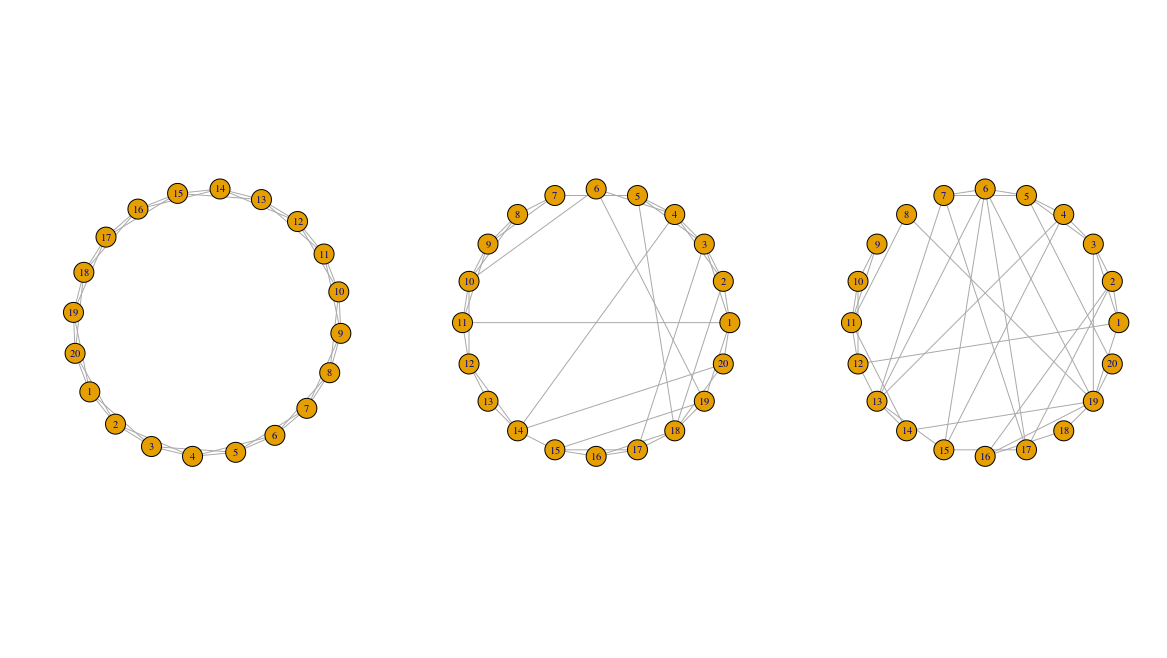
\includegraphics[width=\textwidth]{images/Rplot_corrected_small_world.png}
    \caption{Small world lattice n=20. p of rewiring = 0,0.1,0.3. Code at \url{source('~/RProjects/graph_sw/R/plot_small_world/plot_small_world.R')}}
    \label{fig:small_world}
\end{figure}

\todo{small world network either do here or put in introduction this goes with results }
For results see section~\ref{sec:Results average path length and transitivity}

Bassett \cite{bassett2017small}
\subsection{The configuration model}
\label{sec:configuration model}
\todo{do this}
In considering measures of  a network or a vertex we can study them by seeing how much they differ from their expected value given a random network. Simple random networks such as Erd\H{o}s-R\'enyi random graphs are discussed in the introduction \textcolor{red}{no they aren't} \todo{Erdos Renyi}.

These models however generate networks with a vertex degree distribution that is approximated by  a Poisson distribution (see section~\ref{sec:degree distribution}) \todo{move this to after degree distribution}. Many real world networks have more complicated degree structures such as a power law distribution (see section~\ref{sec:scale_free}) . A number of generating models for power law distribution networks have been described \todo{ref barabasi albert, price}. If one is studying a particular network for which one has the degree sequence then the configuration model is a good choice argues Newman \todo{rephrase}. \cite{newman2018networks}

The configuration model generates a new random network that retains the degree distribution of the original network. Network properties can therefore be compared between the real network and instantiations of the configuration model for that degree distribution. The process for generating the configuration model is a follows: each edge is broken into two stumps and then each of the stumps are rewired in turn into another stump with a uniform probability. This can result in self loops and multiedges\todo{check how multiedges is written in newman}, which do not occur in most real world networks, but the number of these are low as the network size increases \cite{newman2018networks}.




\section{Centrality measures}
\label{sec:centrality measures}
Centrality measures identify important and central nodes in a network \cite{newman2018networks}(p159) based on network topology. This can also be interpreted as a measure of how information flows through a network \cite{borgatti2005centrality} and a variety of measures of importance have been described (see section~\ref{sec: intro_centrality_measures}). These are measures of individual vertices and can therefore be used to rank, group or identify key nodes. Centrality measures are frequently correlated with each other \cite{valente2008correlated} although their correlation varies.\textcolor{red}{move this down}. All measures are derived from the adjacency matrix.\footnote{references for what are 'classic' measures vary \cite{cadini2008using} has closeness, betweenness, information and degree but not eigenvector which most have there is another reference for this but I can't fint it at the moment}



Other vertex measures include eigenvector centrality, a measure of the importance of the node that includes the degree of its neighbours. \cite{bonacich1987power}  Some nodes are bottlenecks in the network. If a large number of the shortest (geodesic) paths pass through a node it is a potential bottleneck and its removal can disrupt the integrity of the network. The measure of a nodes propensity to be a bottleneck is the betweenness centrality. \cite{freeman1977set}. Closeness centrality measures how close a vertex is on average to all other nodes in the network. Transitivity though not a classic centrality measure can be seen as a local form of betweenness centrality \cite{newman2018networks}.

Figure~\ref{fig:dolphin} shows vertex betweenness centrality, eigenvector centrality and local transitivity. High values of these measures are shown in red. The data is from a social network of bottle nose dolphins \footnote{\url{http://www-personal.umich.edu/~mejn/netdata/dolphins.zip}} \cite{lusseau2003bottlenose} \todo{Make vertices bigger in figure}.

\begin{figure}
    \centering
    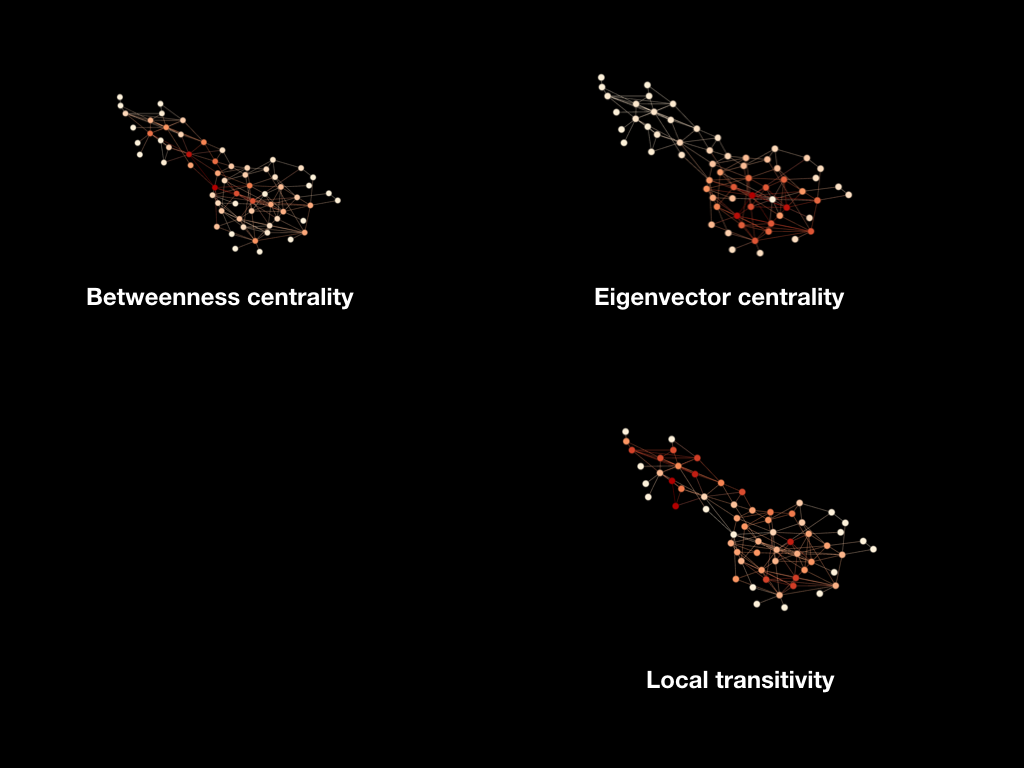
\includegraphics[width=0.9\textwidth]{images/centrality2.002.png}
    \caption{Display of centrality measures. Betweenness centrality, eigenvector centrality and local transitivity for network of bottle nose dolphin social relations data. \cite{lusseau2003bottlenose}}
    \label{fig:dolphin}
\end{figure}

This chapter will consider degree centrality, eigenvector centrality, betweenness, closeness and transitivity in the PSP and their association with animal models of learning and human cognitive ability. \todo{find ref on what are the key centrality measures ?consistency and differences between centrality measures across distinct classes of network}. The simplest centrality measure, degree centrality, \cite{newman2018networks} is considered below. 

\section{Degree centrality}
\label{sec:degree centrality}

%from \url{/home/grant/Dropbox/PhD_latex_master}
The degree of a node is the number of edges connected to it. A node that is connected to a large number of other nodes in a network may be considered central. In a protein interaction network changes in this protein may give rise to a variety of different phenotypes or if the protein is sufficiently essential give rise to severe disease.  In the network graph of the PSP it is the number of proteins a protein (represented by its encoding gene) directly interact with.


Using adjacency matrix $A_{i,j}$, for an undirected, unweighted network such as the PSP,  where $A_{i,j}=1$  if there is an edge between nodes $i$ and $j$ and 0 otherwise, the degree of node $i$, $k_i$ is\cite{boccaletti2006complex}:
\begin{equation}
k_i = \sum_{j=1}^n A_{i,j}.
\label{Equation:Degree_from_adjacency}
\end{equation}

 Nodes with high degree may have more influence in a graph and are often referred to as hubs. \footnote{In a directed network hubs may refer to nodes that point to authorities nodes with important information. As the post synaptic proteome network is undirected hubs will be used in the first sense in this thesis. \cite{kleinberg1999authoritative}}.  In a social network  individuals with many friends a will have a high degree centrality and may be influential in the network. In a protein-protein interaction network high degree proteins will have numerous interactions and one would hypothesise play an important part in the network. 
 
 Disruption of high degree nodes leads to disproportionate effects upon a network \cite{jeong2001lethality} \cite{albert2000error} 


\subsection{Degree distribution}
\label{sec:degree distribution}
The degree distribution of a network is the probability that a particular node has degree $k$. It is a probability distribution and so

\begin{equation}
    \sum_k p(k)=1
\end{equation}.

For an empirical network $P(k)$ is the number of nodes with degree $k$ divided by the number of vertices in the network. 

% An alternative representation for an emprical network is the degree sequence which is  node degree for each vertex in a network eg $1,1,2,3,5,7,\dots,n$. The properties of networks can be discovered by comparing these networks to random models (section~\ref{sec:configuration model}. It seemed reasonable that networks would have degree distributions similar to those found in Erdos Renyi graphs. It was only with the availability of information on large networks such as the internet and world wide web and computerised databases such as the IMDB that the fact that many natural networks have a power law distribution of node degree (section ~\ref{sec:scale_free}. Barabasi, Albert and Jeong found that the internet had a scale free distribution. A narrative of this discovery is provided in Network Science by Barabasi \cite{barabasi2016network}. 


If a graph were to have a  edges distributed between vertices with a uniform probability $p$ we would expect the degree distribution ($P(k)=k)$) to be distributed according to the binomial distribution.  

 The probability of a node having $k$ links is $p^k$, the probability of there being no links to the remaining $N-1-k$ nodes (-1 as we exclude self loops) is $(1-p)^{N-1-k}$ and there are $\binom{N-1}{k}$ ways in which this arrangement of present and missing edges can be arranged. The degree distribution therefore follows the binomial distribution.\cite{barabasi2016network}

\begin{equation}
   \binom{N-1}{k}        p^k (1-p)^{N-1-k}
   \label{Equation:BinomialDistributionForDegreeProbability}
\end{equation}

In the limit where the mean degree is much less than the number of nodes in the network the degree distribution is well approximated by a Poisson distribution \cite{barabasi2016network}. The Poisson distribution

\begin{equation}
    p(k) = \frac{\lambda^k e ^-\lambda}{!k}
\end{equation}

is parameterised for an empirical network only by only by $E[k]$ which is $\lambda$.  The probability mass should be centred around the empirical mean  (17 in the case of the PSP). The variance of a Poisson distribution is $\lambda^{1/2}$ which is approximately 4.12. The top 20 post synaptic proteome genes (table~\ref{Table:The 20 post synaptic proteome genes with highest degree in their cognate proteins} have degree of 221 or greater.  This is not likely under a Poisson model.  \todo{probablility of max degree node} 
\todo{plot of Poisson and empirical for $E[k]$} \textcolor{red}{see figure}


\subsection{Scale free}
\label{sec:scale_free}
% \textcolor{red}{need to give background on barabasi etc}
% \todo{background scale free}
Since 1999 it has been recognised that the degree distribution of nodes in real world networks are commonly scale free \cite{barabasi1999emergence} \cite{barabasi1999mean}. In a scale free network the probability of a vertex having degree $k$ $p(k)$ is:
\begin{equation}
    p(k) \sim k^{-\gamma},
\end{equation}
\label{eq:scale free}

where $\gamma$ is the degree exponent \cite{barabasi2016network}

Power law distributions are called scale free because increasing the value of the degree changes the probability of the degree distribution by a common multiplicative factor. This results in a straight line graph on a log-log plot of degree versus degree distribution. The straight log-log plot has been referred to as the signature of the scale free distribution. 

Many other things in nature follow a scale free distribution (eg size of craters on moon, frequency of words and size of cities) and subsequent research showed that many other networks (the first being the wiring diagram of an IBM chip, the map of the power grid and the Hollywood actor database) are all scale free.\cite{barabasi2016network} \footnote{ p11 in \cite{barabasi2016network}. Chapter 0 of this book gives a detailed personal history of the discovery of the scale free property in networks and its historical antecedents}

Price networks however had been described as a generative model for power law networks in the 1960s. 

Albert, Jeong and Barabasi \cite{albert1999diameter} built a web robot to map out the links in the \url{nd.edu} domain of the world wide web. They found 325729 documents and 1469680 links. In  the world wide web documents point to other documents therefore they constructed a directed graph. The network representing the world wide web displayed a power law distribution with $\gamma_{out}=2.45$ and $\gamma_{in}$=2.1. At that time (1998) there was "no trace in the literature of a network with a power-law distribution". \cite{barabasi2016network}\footnote{p10}

The Barab\'asi-Albert model for generating a scale-free network distribution requires network growth and preferential attachment. Preferential attachment means that new nodes added to the network as it grows tend to be attached to nodes already of high degree.\cite{barabasi1999emergence}

The description of power law distributions remains an eacitve area of research in statistics. Many networks display the power law distribution only in the tails and some conform to log normal distributions. Regardless of this the essential fact is that many real world networks are right skewed with heavy tails and deviate markedly from a Poisson distribution. 




Rare \cite{broido2019scale}







\subsection{Comparison of degree distribution to random erdos graph}
\textcolor{red}{?move to introduction}
See section~\ref{sec: intro_random_graphs}
\todo{Comparison of degree to random graph with same p}

\begin{equation}
    <m> = \binom{n}{2}p
\end{equation}


\begin{equation}
    c = (n-1)p
\end{equation}
where c is the mean degree see newman p 346

Add a histogram here and the expected mean and quartiles.


\subsection{Degree and giant component}
\label{sec:connected component and degree}
\textcolor{red}{ ?move to introduction or second chapter}
Some structure can develop even in random graphs see~\ref{sec: intro_random_graphs}
\todo{Change this as below subcritical, supercritical, fully connected} CHANGE this
In a random graph there is a point at which scattered connected nodes combined to form a giant component. Subcritical to supercritical at $<k> >1$


Supercritical to fully connected at $E[k] > \ln(N)$


Where $N$ is the number of nodes in a network, a giant connected component develops in random graphs when $E[k] > \ln (N)$ \cite{barabasi2016network}. This tends to be the case in real world complex networks. The necessary requirement for a connected component to form is that mean degree is greater than $1/N$. The giant connected component arises in the super-critical' region (see \cite{barabasi2016network} p87). For the PSP $E[k]$ is 17.6 and $\ln(N)=\ln(3457)=8.14$. \todo{this does not follow} It is important to note however that the degree distribution for the PSP graph \textcolor{red}{this does not follow} is not that of a random network ($P(k)$ is scale free it would also be unlikely to find many nodes $ 3 \times E[k]$, if it were there would be few nodes with degree 2 and we find some nodes disconnected from the connected component in our empirical model \todo{so what?}. \todo{cross ref to missing nodes I think it is in the paper section so community detection} \todo{Add plot from \url{'~/RProjects/graph_analysis/R/transitiontoconnectederdosrenyi.R'} for transition from sub-critical to super-critical region} see section~\ref{sec: PSP graph connected component and missing} for missing components.





%%% CENTRALITY MEASURES %%%


\subsection{Betweenness centrality }
\label{sec:Betweeness centrality}
Betweenness centrality and closeness centrality (section~\ref{sec:closenesscentrality})  are both based on shortest paths between nodes.\cite{newman2018networks} Betweenness centrality is a vertex level statistic popularised by Freeman \cite{freeman1977set} \footnote{Newman \cite{newman2018networks} points out that Freeman acknowledges an earlier unpublished account by Anthosine}. It is a measure of the number of geodesic (shortest) paths in the network passing through a particular node. \textcolor{red}{define shortest path} 

 Following Newman's notation \cite{newman2018networks}, if $n_{st}^i$ is one if a shortest path between nodes $s$ and $t$ pass through node $i$ and  $g_{st}$ is the number of shortest paths between $s$ and $t$ (as there may be more than one shortest path) then the betweenness centrality of node $i$ is

\begin{equation}
    x_i = \sum_{st} \frac{n_{st}^i}{g_{st}}.
\end{equation}
\label{eq: Betweenness centrality}

A shortest path exists, in an undirected network, in both directions between a pair of nodes eg from $s$ to $t$ and $t$ to $s$. This double counting does not alter the rank of the nodes ordered by betweenness centrality and allows for easier application to directed networks \cite{newman2018networks}. The betweenness centrality can be normalised by dividing by the number of possible node pairs in the network $n^2$ \cite{newman2018networks} p176

Nodes with high betweenness centrality connect different areas on the network \todo{ref} (ie paths between nodes in the network disproportionately flow through them), and are sites of increased flow (of information for example) assuming that shortest paths are taken through the network \cite{borgatti2005centrality} (compare with random walk betweenness centrality). Other nodes depend on nodes of high betweenness centrality and in the sociological literature they are sometimes referred to as 'brokers' \cite{newman2018networks}. 



\subsubsection{Edge betweenness}
 \todo{edge centrality}
 Edge betweenness centrality is the number of shortest paths that pass through a particular edge \cite{girvan2002community}.

\subsection{Random walk betweenness}
\label{sec: random walk betweenness}
Betweenness centrality assumes that information take the shortest path through the network. This assumption may not be true. Random walk betweenness makes the betweenness metric dependent on the property of random walks in the network. The results are often similar and where they differ it is not apparent what significant should be given to this difference \cite{newman2018networks}

\section{Closeness centrality}
\label{sec:closenesscentrality}
Closeness centrality was described by Alex Bevelas in studies of information flows through social networks \cite{bavelas1948mathematical}. 

Closeness centrality measures how centrally located a node is in a network (ie closeness to all other nodes) to other nodes a node is in the network. Closeness centrality is the inverse of the average length of the shortest path from a node to other vertices in the graph \cite{freeman1978centrality}. $l_i$ is the mean distance between node $i$ and every other node in the network:

\begin{equation}
    l_i = \frac{1}{n} \sum_j d_{ij}.
\end{equation}

 As a \textit{distance} measure it is small when nodes are close to all other nodes. The closeness \textit{centrality} is it's inverse:


\begin{equation}
    C_i = \frac{1}{l_i}. 
\end{equation}
\cite{newman2018networks}

While betweenness centrality measures the dependence of other nodes in the network on a particular node (as a bottleneck for information), the closeness centrality has been interpreted both as proximity and efficient access to other nodes and independence from other nodes \cite{brandes2016maintaining}. Although the meaning given to the measure is different these interpretations are mathematically identical.



\section{Eigenvector centrality}
Degree centrality makes the assumption that connection to a node is  to of equal importance.  A connection to one very important node however may make a node of low degree more important than the increase in degree centrality by one would suggest. 

Eigenvector centrality proposed by Bonacich \cite{bonacich1972factoring} expands on degree centrality and does not consider all of the edges of a vertex equal. Instead if a node is linked to a highly important node this connection is given greater importance. Eigenvector centrality is a measure of the importance of the neighbours of a vertex.

Using Newman's notation \cite{newman2018networks} a nodes importance is defined as the sum of the importance of its neighbours, where $x_i$ is the importance of node $i$

\begin{equation}
    x_i = K^{-1} \sum_j x_j
\end{equation}

$K$ is a constant of proportionality and $j$ denotes all neighbours of node $i$. This can be written using the adjacency matrix as

\begin{equation}
    x_i = K^{-1} \sum_j A_{ij} x_j,
\end{equation}

avoiding the use of $j$ as the neighbours of $x_i$ because the value of the adjacency matrix for nodes $i,j$ that are not neighbours is 0.

In matrix form:
\begin{equation}
    \mathbf{x}=K^{-1}\mathbf{Ax},
    \end{equation}
    
    so
    
    \begin{equation}
         k\mathbf{x}=\mathbf{Ax}.
    \end{equation}
  
This is an eigenvector problem and the vector of centralities is one of the eigenvectors of $\mathbf{A}$. The eigenvector will have as its $i$th entry the importance of the $i$th node. As all centralities should be positive the appropriate eigenvector is the one associated with the largest eigenvalue (by the Perron-Froebenius theorem). 
  
   The values of the eigenvector centrality are not strict measures and we care only for the order of eigenvector centrality. They can however be normalised. 
  
 \section{Related measures}

Katz centrality is a solution to a problem in directed networks. If a vertex is not in a strongly connected component it will have an eigenvector centrality of 0. The Katz centality includes a constant term $\beta$ which is added to the eigenvector centrality and a term $\alpha$ that determines the balance between the eigenvector centrality and the constant term. It is not widely used in undirected networks.\cite{newman2018networks} 

Page rank is a variant of Katz centrality widely used in web-search. Here the benefit of an important neighbour is divided by their out degree (or degree in an undirected network). If I am linked to a very important neighbour, this is much less remarkable if they are also connected to another million people. A review is provided in Gkeik[205]. There are also constant terms $\alpha$ and $\beta$ analagous with katz centrality.\cite{newman2018networks} 
    
% Alpha centrality and bonacich centrality have parameters (bonacich is alpha with alpha preset per bonacich). Bonacich is power\_centrality in igraph. Power centrality with preset is symmetrical around 0. \cite{bonacich1987power}
% Nodes are important if their neighbours are important 
 

% \todo{? add pagerank}




\section{Transitivity}
\label{sec:transitivity}
Transitivity is a measure of how connected the neighbours of nodes are. 
The transitivity of a network measures the probability that two nodes each connected to another node will be in turn connected. If Alice and Bob are both friends with Susan they may be more likely to be friends. The clustering coefficient measures the number of these connections, called \textit{closed triads}, occurring in a network 
divided by the maximum possible.

Transitivity can be calculated for the network as a whole or for individual nodes. This global transitivity sometimes called the clustering coefficient which can be confusing because of the alternate global clustering coefficient described by Watts and Strogatz \cite{watts1998collective} discussed below in section~\ref{sec:Global clustering coefficient}. 

A triangle of vertices,  all connected to each other, forming a loop is  a \textit{closed triad} \cite{newman2018networks}. It is also a path of length two (as paths must have distinct edges). The possible triads that could be formed by the addition of an edge are all paths of length two so the transitivity $C$ is:

\begin{equation}
    C = \frac{\textrm{number of closed paths of length two}}{\textrm{number of paths of length 2}}.
\end{equation}

Since six paths are present in a closed triad (counting once for each direction the path can take in an undirected network eg $ab$ and $ba$ are distinct) the transitivity is:

\begin{equation}
    C = \frac{6 \times \textrm{number of triangles}}{\textrm{number of paths of length 2}}
\end{equation}.

Using \textit{connected triple} to refer to any connected three vertices (whether they form a loop or not) the transitivity can then be expressed as.

\begin{equation}
    C = \frac{6 \times \textrm{number of triangles}}{2 \times \textrm{number of connected triples}}
\end{equation}
The probability the two neighbours of a node in a network are connected is thus its transitivity.\cite{newman2018networks}. 

\todo{expected value compare with random model}


\subsubsection{Global clustering coefficient}
\label{sec:Global clustering coefficient}
The local transitivity defined below (section \ref{sec:local clustering coefficient} is used synonymous with clustering coefficient. The global clustering coefficient however defined by Watts and Strogatz as the arithmetic mean of the vertex local clustering coefficients. The global clustering coefficient can become dominated by nodes of low degree \cite{newman2018networks} p188 and nodes with low degree tend to have high values of local clustering coefficient. 

\subsection{Local clustering coefficient}
\label{sec:local clustering coefficient}
Local transitivity (also known as the local clustering coefficient) is defined as  follows for a vertex having $k_v$ neighbours 

\begin{equation}
C = \frac{c_n}{c_{max}}
\end{equation}
where $c_n$ is the number of connections between a vertexes neighbours and $c_{max}$ is defined as 

\begin{equation}
c_{max} = \frac{k_v(1-k_v)}{2}
\end{equation}

The local clustering coefficient can be regarded as a local inverse of the betweenness centrality \todo{check}. Local clustering measures the connectivity of nodes in the neighbourhood of a particular node. If the local clustering is low then there exist disconnections in a nodes neighbours which are referred to as structural holes \todo{cite ?Burt} the node that connects these neighbours has an importance analogous to that measured by betweenness centrality but confined to the immediate neighbourhood of the node.

\todo{power}





\subsection{kcoreness}

A kcore of a graph is an induced subgraph of the main graph such that each vertex has degree of at least $k$. For a vertex its kcoreness is the maximal k core subgraph it is a member of (alternatively its shell index is $c$ if it belongs to the $c$ core but not the $c+1$ core. \cite{seidman1983network} (original description), \cite{alvarez2006large}. The kcore algorithm is useful in graph analysis as it runs in linear time. It has been used as a measure of core periphery structure in graphs \cite{newman2018networks}\footnote{remove: note to self/JDA its probably one of the easiest one the whole topic of core-periphery is quite complicated and there are several different definitions. The advantage of k-core compared to say the message passing algorithm described by Newman recently for probabilistic core is that it runs in linear time and I could not get the code for Newman to run on anything over 100 nodes}

Humberto used K coreness was used to study the heirarchy of biological networks in plants \cite{humberto2018hierarchical} finding high core metabolic nodes represented core pathways. 

Wuchty examined k core dissection of the protein interactome of Saccharomyces cerevisiae to address the inconsistancies found in the association between lethality and degree . They found a kcore of 9 and that kcore was higher for essential proteins and in those with a eukaryote ortholog \cite{wuchty2005peeling}.

Newman reports that the sociological literature find high k core actors to be important but that the evidence for this is limited.\cite{newman2018networks}

\subsection{Average path length}
\label{sec:Centrality intro average path length}

\section{Assortativity and assortativity of measures}
\label{sec:assortativity}
\textcolor{red}{? move this to the other network level statistics}

\todo{? move along with other network level statistics like small world property, average path length}
Newman described assortativity a network level measure of how likely nodes with similar properties are to be connected. \cite{newman2002assortative} This can be calculated by either scalar or categorical vertex properties.

For a categorical vertex property the calculation is that of the number of edges between vertices that share the property compared with the expected number. This measure is the modularity which we will see again in chapter~\ref{chap:community detection} where the groups are communities. Networks where nodes sharing properties tend to be linked are assortative and those where they are not linked are disassortative

Modularity usually denoted Q is:

\begin{equation}
    Q = \frac{1}{2m}\sum_{ij}(A_{ij}-\frac{k_ik_j}{2m})\delta_{g_ig_j}
\end{equation}

where $m$ is the number of edges in the network, $A$ is the adjacency matrix $k_i$ is the degree of node $i$, $g_i$ is the group or category to which node $i$ belongs and $\delta$ is the Kroneker delta. 

The modularity is less than 1 and takes on a negative value for a disassortative network structure.

The calculation of assortativity for scalar quantities of vertices uses the relationship between the value of the quantity at either end of a connecting edge for all pairs of nodes. This is essentially the covariance and the measure the assortativity coefficient is the covariance normalised by the maximal value of the covariance or variance of the measures for each node \todo{review}

\subsection{Degree assortativity}
\label{sec:degree assortativity}

The most commonly studied scalar property is degree association \cite{newman2018networks}p210. The degree assortativity is the Pearson correlation between degree for connected vertices.\cite{noldus2015assortativity}. Assortative networks tend to form communities and are more robust to disruption by node removal  \cite{newman2002assortative} and increased assortativity leads to increased speed of transmission of information through a graph \cite{noldus2015assortativity}.

Social networks tend to be assortative with a core structure of highly connected hubs. \cite{newman2018networks}
\todo{plot of knng and deg at\url{source('~/RProjects/correlation_gene_scores/R/make_df_graph_stats_correlation_lowdeg_high_bet.R')}} although there seems to be a very weak correlation between knn and z score. 



\subsection{Other measures}
\subsubsection{Shortest paths}


\subsubsection{Bridging}

\cite{valente2010bridging}

%%%%%%%%%%%%%%%%%%%%   CENTRALIY IN BIOLOGY AND MEDICINE %%%%%%%%%%%%%%%%%%%%%%%%%%%%%%%%%%%%%%%%%%%%%%%%%%%%%%%%%%%%%

\section{Biomedical significance of centrality measures}

 High degree nodes are called hubs and proteome hub proteins are known to be more commonly essential to life \cite{jeong2001lethality} and expressed ubiquitously. \cite{goh2007human}  Jeong found that high degree nodes in yeast were more likely to be essential to life \cite{jeong2001lethality} although later work has questioned this (see section\todo{cross ref} Unregulated\todo{check unregulated or upregulated} genes in cancer proteomic networks have been found to be of high degree. \cite{wachi2005interactome}  High degree nodes were  involved in more diseases in the Online Mendelian Inheritance in Man (OMIM) compendium of genetic phenotypes. \cite{xu2006discovering}  Goh however found that disease genes were likely to be tissue specific and were not more likely to be hubs. \cite{goh2007human}  
 
High degree hub genes are more likely to be essential rather than disease genes \cite{barabasi2011network}. 

Lee et al. \cite{lee2013network} in 2013 examined National Human Genome Research Institute (NHGRI)  catalogue of complex trait GWAS \footnote{now the NHGRI-EBI GWAS catalogue} and found that complex trait loci were more likely to be found in genes that were hubs or bottlenecks, where hub and bottleneck are defined as the top 20\% of the degree centrality and betweenness centrality distribution.  The network is composed of the genes encoding protein protein interactions in the STRING (14025 nodes and 492087 edges representing protein protein interactions). The GWAS datasets were composed of type 2 diabetes studies (FUSION  Cases n=	1161 Controls n=	1174 
WTCCC Cases n=	2000 controls n=	3000  and Inflammatory Bowel Disease Genetics Consortium (IBDGC) with European populations without Jewish ancestry and those with Jewish ancestry (IBDGCi case n=	561 control n=	563 IBDGCii case n= 	407 control n=	432).  

Liu \cite{liu2017sigmod} described a method of identifying gene modules and combining this with p values but use heterogenous different measures of gene interaction including coexpression from the STRING database version 10 which results in what they refer to as a GeneNet \todo{there is a thing called a gene net - check} with 19 247 genes and 4 274 001 edges. Edges are given weights based on level of evidence but if there is a connection but no weighting a value of 1 is given. Nodes are given higher significance based on degree.  Gene level P values were obtained by calculating the value of the top SNP within a gene. They compare their results to two other methods dmGWAS and SCoNEs. Their method is implemented in an R module (SigMod) last updated 2 years ago \todo{remove this this is to jog my memory}. They appear to use a min cut algorithm to find modules and take into account degree. THere is also a complex method for adjusting two tunable parameters \todo{can't really make head or tail of this paper. Don't know why they didn't use something like VEGAS. }



\cite{bayes2011characterization} found strong sequence conservation in PSP hub proteins. So there is some evidence that we might suspect they have an influence on human cognition using the G2C framework but as this is complex what we need is empirical proof indeed one can make a plausible argument from the available evidence for the effect of a specific measure, for an effect of centrality generally or for no effect \todo{? add box}.  


\subsection{ Biomedical Review}
Ghasemi provides a review of centrality measures in biological networks as of 2014 and illustations of each centrality measure on Zacharys Karate network.
\cite{ghasemi2014centrality}. Some of the papers cited are discussed below but the reader is directed to Ghasemi \cite{ghasemi2014centrality} for a fuller review. 

Hahn and Kern\cite{hahn2005comparative} examined protein protein interactions networks in fly, yeast and worm measuring betweennness centrality, degree centrality and closeness centrality. They found that more centrally located proteins in all networks evolved more slowly. 

Ozgur \cite{ozgur2008identifying} developed a curated gene interaction network and used centrality measures to attempt to predict the genes association with prostatic cancer using the prostate gene database (PGDB). They measured degree, eigenvector, betweenness and closeness centrality and found that high scores on the first three measures were increased in increased confidence in rank in the PDGB.

Estrada \cite{estrada2006virtual} used centrality meassures to assess essentialness in the yeast protein interaction network (degree centrlity, eigenvector centrality, information centrality, closeness centrality, betweenness centrality and subgraph centrality. They found that high centrality measures predicted essentialness better than random selection and  the best results were obtained using eigenvector centrality and the poorest using closeness and betweenness centrality. 

Joy found that nodes with high betweenness and low degree centrality were particularly abundant.\cite{joy2005high} in Yeast protein protein interactin (this does not seem to be the case in our data see \url{lm_1 <- lm_1 <- lm(ZSTAT ~  eig*scale_bet*I(1/scale_deg),data=ukbb_int_df2)}

Pandey analysed GWAS results for bipolar disorder using eigenvector centrality \cite{pandey2012epistasis}. They used the WTCCC-BD GWAS (1868 cases and 2938 controls) as a discovery sample and  a NIMH GWAS (1001 cases; n=1033 controls) of individual of european ancestry as replication. Having constructed an epistasis network they used eigenvector centrality to rank the 1000 nodes in the SNP epistasis network and then assessed what pathways were enriched for the ranked SNPs. The network was a statistical network described as reGAIN (regression based genetic assocation network) where edges are statistical interactions \todo{i presume}\footnote{they have a previous method based on information gain The analysis is limited by the lack of power provided by the sample size available.}

\section{Degree and essentialness Introduction}
\label{sec:Degree and essentialness}
Jeong \cite{jeong2001lethality} examined the correlation between a gene being essential and having high degree in the proteome of \textit{Saccharomyces ceresvisiae} having 1870 nodes and 2240 interactions (comparatively sparse compared with the synaptic proteome). They found that elimination of the most connected nodes led to an increase in network diameter and that the likelihood that mutation in a protein would prove fatal was correlated with degree, They found that 21\% of the nodes with degree less than 5 (93\% of the proteome) had lethal effects from mutation. Although 0.7\% of yeasts had more than 15 links  62\% of these had lethal phenotypes. However later work with more complete networks did not support this \cite{milenkovic2011dominating} \cite{yu2008high} \cite{ratmann2009evidence}

More recent high quality yeast interactomes however have not shown evidence of this effect \cite{milenkovic2011dominating}, \cite{yu2008high}, 

p53 
Raman \cite{raman2014organisational} examined multiple centrality metrics in addition to degree (degree, betweenness centrality, closeness centrality and pairwise dis-connectivity index) and their association with gene essentiality for 20 organisms.

 Using the STRING database filtered for high quality interactions they found a disassortative \todo{ this suggests you need to put assortativity in the introduction bit} pattern of connection of essential genes (they did not appear to be connected to each other)  (compare with section~\ref{sec:degree assortativity})  and found higher than average degree and betweenness centrality (greatest for degree centrality). The organisms that they studied (20) were mostly bacteria and yeasts, no most sophisticated I could see was \textit{Caenorhabditis elegans}.\todo{rephrase} They also calculated what fraction of essential nodes had a higher degree than n where n is a centile of the degree distribution).


\textcolor{red}{there is\subsection{Centrality and intelligence in PSP}
We will see what the correlation is in population cohorts and what we might expect it to be given the effects of high degree genes in model animals. Essentially nobody knows \todo{rephrase}
\todo{This is perhaps the bit to introduce the possible different hypothesise} a note betweennness and transitivity and betweeness and biological illegible maybe literature}
 
%%%%%%%%%%%%%%%%%%%%%%%%%%%    METHODS  %%%%%%%%%%%%%%%%%%%%%%%%%%%%%%%%%%%%%%%%%%%%%%%%%%%%%

%%%%%%%%%%%%%%%%%%%%%%%%%%%    METHODS  %%%%%%%%%%%%%%%%%%%%%%%%%%%%%%%%%%%%%%%%%%%%%%%%%%%%%

%%%%%%%%%%%%%%%%%%%%%%%%%%%    METHODS  %%%%%%%%%%%%%%%%%%%%%%%%%%%%%%%%%%%%%%%%%%%%%%%%%%%%%

%%%%%%%%%%%%%%%%%%%%%%%%%%%    METHODS  %%%%%%%%%%%%%%%%%%%%%%%%%%%%%%%%%%%%%%%%%%%%%%%%%%%%%

%%%%%%%%%%%%%%%%%%%%%%%%%%%    METHODS  %%%%%%%%%%%%%%%%%%%%%%%%%%%%%%%%%%%%%%%%%%%%%%%%%%%%%

%%%%%%%%%%%%%%%%%%%%%%%%%%%    METHODS  %%%%%%%%%%%%%%%%%%%%%%%%%%%%%%%%%%%%%%%%%%%%%%%%%%%%%

%%%%%%%%%%%%%%%%%%%%%%%%%%%    METHODS  %%%%%%%%%%%%%%%%%%%%%%%%%%%%%%%%%%%%%%%%%%%%%%%%%%%%%

\section{METHODS}

\subsection{Methods Fitting the degree distribution - scale free property}

We can calculate the $\gamma$ coefficient for the degree distribution using the \texttt{poweRlaw} package for R. The value of $\gamma$ will vary over the distribution depending on the lower limit of degree used to fit the power law distribution. This is shown graphically in figure \ref{fig:gamma} and table \ref{table:gamma}.

A power law distribution may not hold throughout a distribution it is typically present at the tail (high degree) of the degree distribution. There is therefore a minimum value of degree from which the power law distribution holds (there is also frequently dispersion at the end (high) of the distribution. The characteristic feature of a power law degree distribution is a straight line in a log-log plot of $ P(k)$ and $k$.

The minimum degree in which the power law distribution is found is calculated such that it minimises the difference between the network degree distribution and the best fitted power law distribution. The distance between the distributions is measured by a Kolmogorov-Smirnov statistic in the method described by Clauset, Shalizi and Newman \cite{clauset2009power} section 3.3 p 11-12  following earlier work by the first author \cite{clauset2007frequency} \footnote{interestingly in the frequency of terrorism incidents}. 

The method is implemented in the \texttt{poweRlaw} package for R \cite{gillespie2015fitting}\footnote{see page 7 in \url{https://cran.r-project.org/web/packages/poweRlaw/vignettes/a_introduction.pdf} for a clear description of the implementation}.

Recent research has suggested that power law distributions may be rare in empirical networks and a log normal distribution may be a better fit. The log normal is still a significant deviation from the Poisson distribution that would be seen in a random graph generated with uniform probability of connection. I have calculated the log likelihood of the log normal, power law and Poisson distribution. As we log likelihood is affected by the number of data points I report the fit of the log-normal \footnote{note to self clauset and newman use log-normal} and Poisson over the same degree range as the power law\footnote{note to self Newman uses power law not power-law remove any different} fit. The log likelihood calculations were carried out using the \texttt{poweRlaw} package for R \cite{gillespie2015fitting} using the \texttt{dist\_ll} method for distribution objects fitted to the data using the above distributions (for example \texttt{power\_law\_object = displ\$new(data)} for a power law distribution to the data for which the minimum degree and exponent would then be it) \todo{p21 of Clauset-Newman suggests using method of Vuong}

\footnote{p 17 rule out powerlaw on bootstrap p if $p<=0.1$ p large when good fit}


\section{Methods Gene ontology enrichment}
\label{sec:Methods gene ontology centrality}
\textcolor{red}{Cross ref to bit in next section or bring it here 4.16.5}  

See section~\ref{sec: gene ontology analysis}.
To understand the properties of nodes of different centrality's we performed gene ontology enrichment both with the background of the PSP and against the whole of the genome where the whole of the genome is defined as genes appearing in at least one of the cohort studies \todo{add cross ref}

\todo{Panther}
\todo{background}
\todo{Fishers test}
\todo{topgo}


\subsection{Methods GO Slim}
\textcolor{red}{Define}

\subsection{Methods and results global clustering coefficient}
Calculations of local transitivity were carried out using the transitivity method in \texttt{igraph} for R with the argument type being global undirected. Local transitivity was carried out using transitivity with the type being local transitivity is not defined for nodes of degree 0 so as an alternate to NA the argument isolates="zero" was used. 

\subsection{Methods Murine LTP and centrality}
Identification of murine genes associated with LTP and testing of LTP and centrality. For results see section \ref{sec:results centrality and murine models of long term potentiation}.\todo{murine ltp}

%%%%%    Methods essentialness %%%%%%%%%%%%%%%%%%%%%%%%%%%%%%

\section{Centrality and essentialness}
To test the centrality lethality hypothesis for human population in the PSP and to investigate whether genes associatioed with differences in intelligence were under purifying selection (see chapter \todo{add cross ref to communities chapter} we used the database of eessential genes and the Exac database. 

\subsection{Database of essential genes Methods}
 \label{sec:Database of essential genes}
 
 To obtain a list of essential human genes we used the database of essential genes (DEG).\cite{luo2014deg}. The database of essential genes (DEG) is found at \url{www.essentialgene.org}.The most up to date database was still under preparation on 09th June 2020 but the previous version is available at \cite{ http://tubic.org/deg_bak/}. We used the most up to date version available DEG 15.2 (Dec 18, 2017). Data on essential genes is available for bacteria, archaea, eukaryotes and non-coding.
 
  Downloading essential eukaryote genes (\url{http://tubic.org/deg_bak/download/deg-e-15.2.zip}) yields 34590 entries. Columns are DEG Accession and  accession number, Gene symbol, gene ref (Gen Bank GI number see \url{https://www.ncbi.nlm.nih.gov/genbank/sequenceids/}, COG (all blank), Functional Class (14 including undefined), Function, Organism, Refseq and Condition. Gen Bank GI number is not recorded for humans.
  
  For humans EMBLENSG is avialable, Chromosome location (V9), V11 ENSG and symbol V13 Protein ID, V14 HGNC number
%  [1] "-"                                        "Ergosterol biosynthesis"                  "Protein transport"                       
%  [4] "Amino acid biosynthesis"                  "Component of 90S preribosomal particles"  "Cellular metabolism"                     
%  [7] "Protein translation"                      "Ribosome biogenesis"                      "Cytoskeleton organization and biogenesis"
% [10] "Cell wall organization and biogenesis"    "RNA splicing"                             "Cell redox homeostasis"                  
% [13] "DNA replication"                          "Protein modification"                    
 Data is available for 9 organisms:  Saccharomyces cerevisiae   ,Caenorhabditis elegans,Arabidopsis thaliana,Danio rerio,Mus musculus,Homo sapiens,
 Drosophila melanogaster,Aspergillus fumigatus and Schizosaccharomyces pombe 972h-.
 
 Data on 34590 genes are recorded. 
 Data on 28286 \todo{is this correct this is more than the number of protein coding genes?} human genes are recorded. 8256 unique gene symbols are found for human genes. 8214 unique hgnc id numbers  , ENSG 12947 Human genes, 8168 unique proteins  are identified by UniProtKB  \footnote{\url{source('~/RProjects/paper_xls_latex/R/essentail_genes/load_essential_genes.R')}}.
 
 The pattern of duplicated data was complex for example 118 HGNC id were unrecorded (recorded as "-", the next commonest was one with 15 duplicates). Most of the 
 
 Entrez id were obtained using the module \url{convert_gmx_private}\footnote{ at \url{/home/grant/PycharmProjects/convert_gmx_private}}.
 
 This uses downloaded gene info from entrez gene to find first the symbol and if that is missing to search through synonyms and supply the matching entrez id. It returns a list of items not found. 
 
8284 genes were translated to entrez id. 8236 of these were unique (from 8256) 8 ids could not be identified. 3 of these are recorded as dates in the primary data \footnote{(5,6 Mar, 5 Sep)}
 
 The dataframe of conversions are stored in the supplemental data\footnote{ \url{/home/grant/RProjects/paper_xls_latex/data/essential_genes.tsv}}
\subsection{Loss of function and evolutionary pressure}

The Exac database is a compendium of data from the exomes of over 60,000 individuals \cite{lek2016analysis}. It allows the calculation of the tolerance to mutation of in specific genes. By comparing the number of loss of function mutations to those expected given the number of synonymous mutations we can identify if there is a lack of mutations in the population in a specific region and can conclude that the organism is intolerant to such mutations. The researchers provide a statistic the probability of loss of function intolerance that provides a measure of how much purifying selection a gene is under. 

The file was downloaded from 
\url{"https://storage.googleapis.com/gnomad-public/legacy/exac_browser/forweb_cleaned_exac_r03_march16_z_data_pLI_CNV-final.txt.gz"} (valid on 16.06)

\subsubsection{Processing and cleaning Exac data for PSP}
\todo{query move to supplemental methods}
The data consists of 18282 rows and 23 columns. A variety of metrics are available to measure the frequency of synonymous mutations, non synonymous mutations and missense mutations. The authors recommend the use of the probability of loss of function mutation metric as this takes into account variations in gene size which some other metrics may be biased by. In addition the rows were identified by Ensembl transcript ID, HUGO gene symbol and contained information on the number of base pairs, chromosome number and location on the chromosome. This data is recorded in supplementary section~
\ref{sec:supplemental data table for exac}.


% raw output for ref
%[1] "gene"       "chr"        "n_exons"    "tx_start"   "tx_end"    
% [7] "bp"         "mu_syn"     "mu_mis"     "mu_lof"     "n_syn"      %"n_mis"     
%[13] "n_lof"      "exp_syn"    "exp_mis"    "exp_lof"    "syn_z"      "mis_z"     
%[19] "lof_z"      "pLI"        "n_cnv"      "exp_cnv"    "cnv_z"     
% end
114 entries were found to have duplicated Ensembl transcript id. These were entries with differing cnv count. Each duplicate was duplicated twice (57 unique ensembl ids).see table~\ref{tab:Supplementary table- duplicate exac data}. Code to download the database and check these items only differ in cnv count is at \url{source('~/RProjects/paper_xls_output/R/exac_check_for_duplicates_mod.R')} and
\url{source('~/RProjects/paper_xls_output/R/download_exac.R')}As the data differed only in cnv number and cnv number was not part of the analysis one copy was discarded resulting in n=18225 entries. 

%  \textcolor{red}{this matches the redo}\footnote{code \url{('~/Rprojects/paper_xls_output/R/download_exac.R')}}.

Human entrez id was downloaded from
\url{"ftp://ftp.ncbi.nih.gov/gene/DATA/GENE_INFO/Mammalia/Homo_sapiens.gene_info.gz"} and processed using an Rscript \url{source('~/RProjects/paper_xls_output/R/download_to_dataframe_geneinfo.R')} to remove \# symbols denoting comments. 



% The genes were identifiable from both transcript ID ENST, and HGNC gene symbol. (18282 - 57) 18225 distinct transcripts and gene symbols were identified.

% 57 transcript id and gene ID were duplicated and removed  There were 114 duplicated entries (i.e. each was duplicated twice). For all duplicates all statistics were identical of than number of copy number variations, expected number of copy number variations and z score for copy number variations. 
% \todo{move into separate function}

% As we were not using CNV these were eliminated
Entrez ID were obtained for the Exac data by mapping the  HUGO gene symbol provided using Entrez gene info. This joined table has 8 duplicates as a result of Exac gene symbols mapping to more than one entrez ID)
\url{source('~/RProjects/paper_xls_output/R/download_and_cleanexac/exac_check_for_duplicates_mod.R')}
\footnote{variable is
\texttt{joined\_duplicatez}}
\todo{this as a table}
% latex table generated in R 3.6.3 by xtable 1.8-4 package
% Tue Jun 16 17:18:02 2020
\begin{table}[ht]
\centering
\begin{tabular}{rlllrrl}
  \hline
 & transcript & gene & chr & pLI & GeneID & description \\ 
  \hline
6707 & ENST00000380299.3 & HBD & 11 & 0.00 & 3045 & hemoglobin subunit delta \\ 
  6708 & ENST00000380299.3 & HBD & 11 & 0.00 & 100187828 & hypophosphatemic bone disease \\ 
  9176 & ENST00000295065.5 & MEMO1 & 2 & 0.88 & 7795 & Methylation modifier for class I HLA \\ 
  9177 & ENST00000295065.5 & MEMO1 & 2 & 0.88 & 51072 & mediator of cell motility 1 \\ 
  9365 & ENST00000404774.3 & MMD2 & 7 & 0.00 & 221938 & monocyte to macrophage differentiation associated 2 \\ 
  9366 & ENST00000404774.3 & MMD2 & 7 & 0.00 & 100505381 & Miyoshi muscular dystrophy 2 \\ 
  15629 & ENST00000381501.3 & TEC & 4 & 0.00 & 7006 & tec protein tyrosine kinase \\ 
  15630 & ENST00000381501.3 & TEC & 4 & 0.00 & 100124696 & transient erythroblastopenia of childhood \\ 
   \hline
\end{tabular}
\caption{Supplemental Duplicated Gene symbol to gene id mapping for Exac}
\label{tab:supp duplicated gene symbol for exac entrez}
\end{table}



Code for the extraction and processing of the loss of function intolerance data was as follows 
\url{~/RProjects/paper_xls_output/R/download_exac.R}

For 17084 genes an entrez id could be matched with the supplied HUGO symbol but for 1141 genes an entrez id could not be identified. 

There are 17928 entrez id in all gene studies
15989 of these represented in the Exac data with an entrez id
89.2\%. 16277 entrez id are found in the list of entrez id occurring in any study 18390 88.2\%. 3235 genes of the PSP have exac data (93.6\%). The missing 222 have insufficient coverage by searching the Exac browser. The missing ones are shown in supplemental table x\todo{do this table}. The availability of Exac data matched to an entrez id is shown in table~\ref{tab:exac_coverage}

Lookup on \url{https://grch37.ensembl.org/Multi/Search/Results?q=ENST00000404774.3;site=ensembl_all}

\begin{table}[]
    \centering
    \begin{tabular}{llll}
    \toprule
      Description   & Exac data with entrez id & N genes & Percentage coverage  \\
      \midrule
      All non duplicated exac data  & 17084 & 18225 & 93.7\\
       Genes present in all samples  & 15989 & 17928 & 89.2\\
       Genes present in at least one sample & 16277 & 18390 & 88.2\\
       Post synaptic proteome genes & 3235 & PSP size & 93.6\\
       \bottomrule
    \end{tabular}
    \caption{Availability of Exac data with identifiable entrez id. Coverage of GWAS studies (Education and Intelligence) discovery and replication and of Post synaptic proteome. The difference between the number in all non duplicated exac data and genes present in GWAS samples is that some genes do not appear in the exac database having insufficient coverage}
    \label{tab:exac_coverage}
\end{table}

(for missing id please see section below)



\todo{at this point commented out duplicates as text}

% MEMO1 mediator of cell motility Entrez 7795 (Methylation modifier for class I HLA
% ) and 51072(correct)

% MMD2 monocyte to macrophage 221938 MMD2 100505381 (Miyoshi Muscular Dystrophy 2 – wrong)

% TEC tec Protein tyrosine kinase 7006 not 100124696 (Transient erythroblastopaenia of childhood)

% One synaptic gene is found in the duplicated list HBD Gene ID 3045 which also has the entrez ID 100187828 
% HBD
% the transcript is ENST00000380299.3 which is haemaglobin delta maps to ENSG00000223609

% there is also Hypophosphataemic bone disease which is 100187827 but the one that is present in the synapse is 3045
% There are 14990 non synaptic genes with exac information and a total of 18225 \textcolor{red}{18070 in redo} genes with exac gene info


 \todo{should look like}
 \textcolor{red}{ Genes reomved. N synaptic. N other. N duplicated. N missing. Flowchart and table for duplicates (then move table to supplemental)}

\subsubsection{Use of Exac data}

We calculated the Spearman's rank correlation between loss of function intolerance and centrality scores and with GWA scores. Calculations for correlation coefficient were carried out in R. The distribution of centrality measures and pLI deviated from a normal distribution. 

\todo{cross ref non normality of centrality measures and do shapiro wilk for pli}

Code for calculating correlation of gene score with pLI at \url{source('~/RProjects/paper_xls_output/R/make_pLI_correlation.R')}
\todo{Modify to add closeness}
\section{Cohorts and samples}
\label{Centrality:cohorts and samples}
\todo{do correlation centrality with murine ltp group}
The population data used to test the association of centrality measures with population studies of educationbal attainment and intelligence were those described in sections~\ref{sec:cohorts from paper section} and \ref{sec:samples from paper section}

\subsection{Calculating centralities}
Eigenvector centrality is implemented in igraph for R by the \texttt{eigen\_centrality} function taking the graph as the argument.


\todo{Add introduction}


%%%%%%%%%%%%%%%%%%%%%%%%%%%    RESULTS  %%%%%%%%%%%%%%%%%%%%%%%%%%%%%%%%%%%%%%%%%%%%%%%%%%%%%

%%%%%%%%%%%%%%%%%%%%%%%%%%%    RESULTS  %%%%%%%%%%%%%%%%%%%%%%%%%%%%%%%%%%%%%%%%%%%%%%%%%%%%%

%%%%%%%%%%%%%%%%%%%%%%%%%%%    RESULTS  %%%%%%%%%%%%%%%%%%%%%%%%%%%%%%%%%%%%%%%%%%%%%%%%%%%%%

%%%%%%%%%%%%%%%%%%%%%%%%%%%    RESULTS  %%%%%%%%%%%%%%%%%%%%%%%%%%%%%%%%%%%%%%%%%%%%%%%%%%%%%

%%%%%%%%%%%%%%%%%%%%%%%%%%%    RESULTS  %%%%%%%%%%%%%%%%%%%%%%%%%%%%%%%%%%%%%%%%%%%%%%%%%%%%%

%%%%%%%%%%%%%%%%%%%%%%%%%%%    RESULTS  %%%%%%%%%%%%%%%%%%%%%%%%%%%%%%%%%%%%%%%%%%%%%%%%%%%%%

%%%%%%%%%%%%%%%%%%%%%%%%%%%    RESULTS  %%%%%%%%%%%%%%%%%%%%%%%%%%%%%%%%%%%%%%%%%%%%%%%%%%%%%



\section{RESULTS}
? divide into graph level and vertex level
\todo{? divide into graph level and vertex level}

\section{Summary of centrality measures}

The summary values for the centrality measures are shown in table \ref{Table:Summary of centrality measures}. The transitivity contained 304 NA's.
\todo{add graph}
The eigenvector centrality and transitivity are normalised. For some nodes the transitivity cannot be calculated (those of degree 1). There are 304 of these and the summary statistics are calculated excluding these values\footnote{an alternative is to set them to zero}. 

The centrality measures are not normally distributed see table~\ref{Table:Test for normality (Shapiro-Wilk) for centrality measures of PSP}.



\footnote{\url{source('~/RProjects/paper_xls_latex/R/centrality_summary/centrality_summary_latex.R')}}
% latex table generated in R 3.6.2 by xtable 1.8-4 package
% Mon Feb 10 14:17:12 2020
\begin{table}[ht]
\centering
\begin{tabular}{rrrrrrr}
  \hline
 & Minimum & 1st Quartile & Median & Mean & 3rd Quartile & Maximum \\ 
  \hline
Degree & $1 $ & $4 $ & $8 $ & $17.64$  & $19$ & $535$ \\ 
  Eigenvector & $1.821 \times 10^{-6}$ & $8.829 \times 10^{-3}$ & $2.194 \times 10^{-2}$ & $4.793 \times 10^{-2}$ & $5.322 \times 10^{-2}$ & $1 $ \\ 
  Betweenness & $0 $ & $43.29 $ & $317 $ & $3421.1$ & $1571.6$& $6.447 \times 10^{5}$ \\ 
  Transitivity & $0 $ & $4.376 \times 10^{-2}$ & $1.290 \times 10^{-1}$ & $1.714 \times 10^{-1}$ & $2.381 \times 10^{-1}$ & $1 $ \\ 
  Closeness & $5.702 \times 10^{-5}$ & $9.217 \times 10^{-5}$ & $9.879 \times 10^{-5}$ & $9.845 \times 10^{-5}$ & $1.058 \times 10^{-4}$ & $1.399 \times 10^{-4}$ \\ 
   \hline
\end{tabular}
\caption{Summary of centrality measures} 
\label{Table:Summary of centrality measures}
\end{table}
\todo{Global transitivity and compare}
\todo{query pull out the global measures eg degree assortativity, transitivity}


\begin{table}[h]
    \centering
    \begin{tabular}{c|c|c}
       Centrality measure  &  W& p\\
       \hline
       
       Degree  & 0.426 & $<2.2 \times 10^{-16}$ \\
       Eigenvector &0.561  & $<2.2 \times 10^{-16}$ \\
       Betweenness &0.1228& $<2.2 \times 10^{-16}$ \\
       Transitivity &0.782 & $<2.2 \times 10^{-16}$\\
       Closeness &0.9953& $<4.686 \times 10^{-09}$\\ 
    \end{tabular}
    \caption{Test for normality (Shapiro-Wilk) for centrality measures of PSP}
    \label{Table:Test for normality (Shapiro-Wilk) for centrality measures of PSP}
\end{table}

\section{Correlation of centrality measures}

A scatterplot of the relation of centrality measures is shown in figure~\ref{fig:scatter plot of multiple centrality measures}.

\begin{figure} 
    \centering
    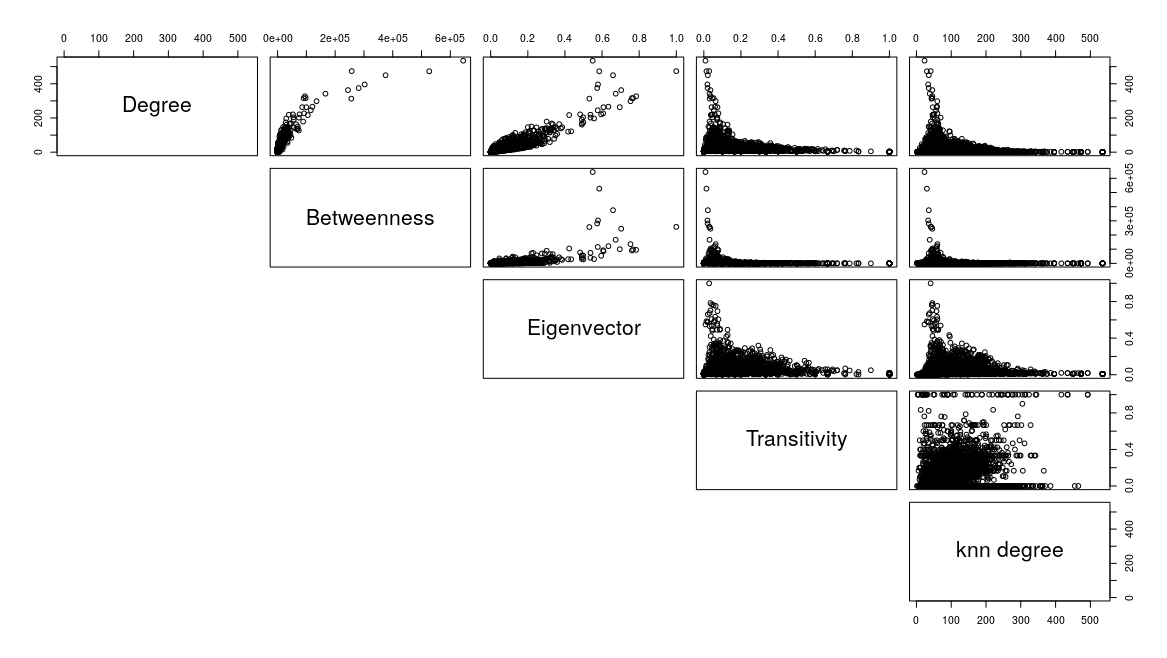
\includegraphics[width=\textwidth]{images/Rplot_pairs_plot.png}
    \caption{Scatter plot of centrality measures. Source \url{source('~/RProjects/correlation_gene_scores/R/make_df_graph_stats_correlation_lowdeg_high_bet.R')}}
    \label{fig:scatter plot of multiple centrality measures}
\end{figure}
\subsection{RESULTS Scale free}
Using the method described by Clauset and Newman \cite{clauset2009power} and calculating the minimum x value we find the min for $x$ to be 24 and the $\gamma$ coefficient to be 2.51 using the poweRlaw R package \cite{gillespie2015fitting}. GOF 0.19. ntail 68 \footnote{\url{source('~/RProjects/group_size_distribution/R/calulate_cdf.R')}} The log of the degree distribution is shown in figure \ref{fig:log_degree_distribution} and figure \ref{fig:Degree distribution of post synaptic proteome. Log10 - log10 scale.}
% see http://127.0.0.1:21133/library/poweRlaw/doc/a_introduction.pdf
\footnote{code at \url{/home/grant/RProjects/PhD_graphs/}}


The bootstrap p for the power law distribution is 0.583 with goodness of fit 0.19 using the package poweRlaw 0.70.6 using ks distance.\footnote{\url{source('~/RProjects/group_size_distribution/R/calulate_cdf.R')}}

To determine the best distribution calculated the log likelihood of the distribution given power law, log normal and poisson distribution. To allow comparison of the log likelihood the likelihood was calculated for the data from the $x_min$ determined for the powerlaw distribution $x_min = 24$. See table~\ref{tab:log likelihood powelaw}

\begin{table}[]
    \centering
    \begin{tabular}{cc}
    Distribution     &  log likelihood \\
    \hline
     Power law    & -2943.6\\
     Log normal & -2947.23 \\
     Poisson & -205115.8 \\
    \end{tabular}
    \caption{Log likelihood of degree distribution using poweRlaw package with $x_{min}=24$ for power law distribution and log normal and poisson.\url{source('~/RProjects/group_size_distribution/R/side_by_side_lognorm_and_pl.R')}}
    \label{tab:log likelihood powelaw}
\end{table}

\begin{figure}
    \centering
    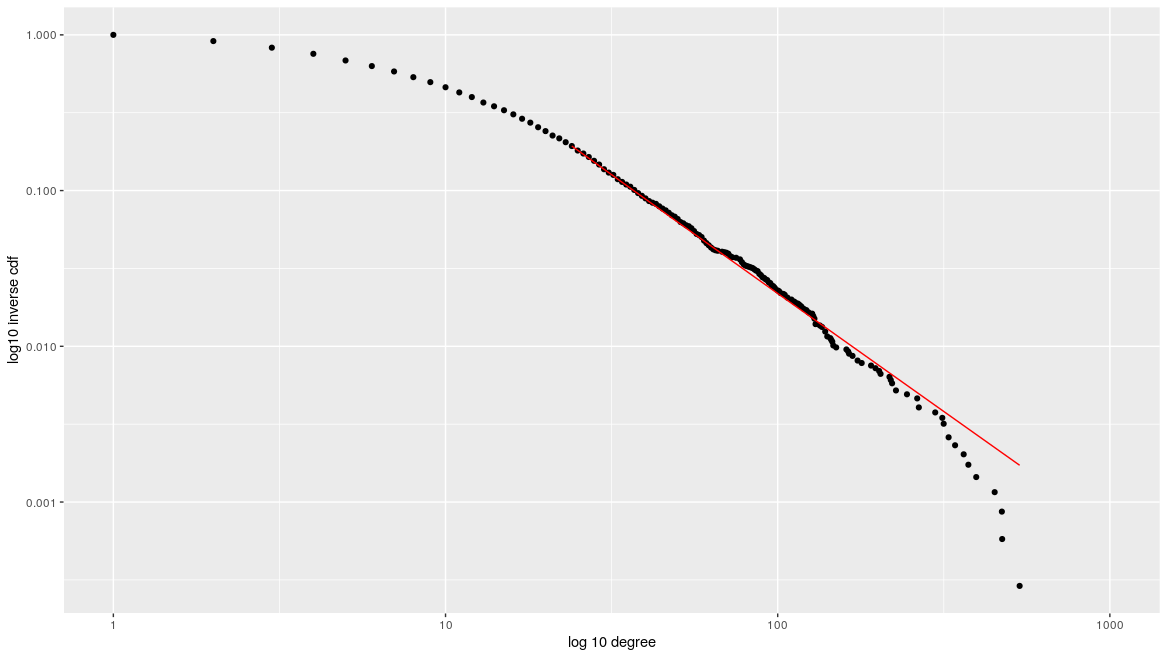
\includegraphics[width=\linewidth]{images/Rplot01_poweRlaw_ggplot.png}
    \caption{Plot of fit of power law to degree distribution for the PSP. X axis is log 10 degree, Y axis is log 10 inverse cdf. Red line fit of power law distribution $\gamma= 2.51$ and $x_{min}=24$ \url{source('~/RProjects/group_size_distribution/R/calulate_cdf.R')}}
    \label{fig:poweRlaw plot ggplot2}
\end{figure}




\begin{figure}
    \centering
    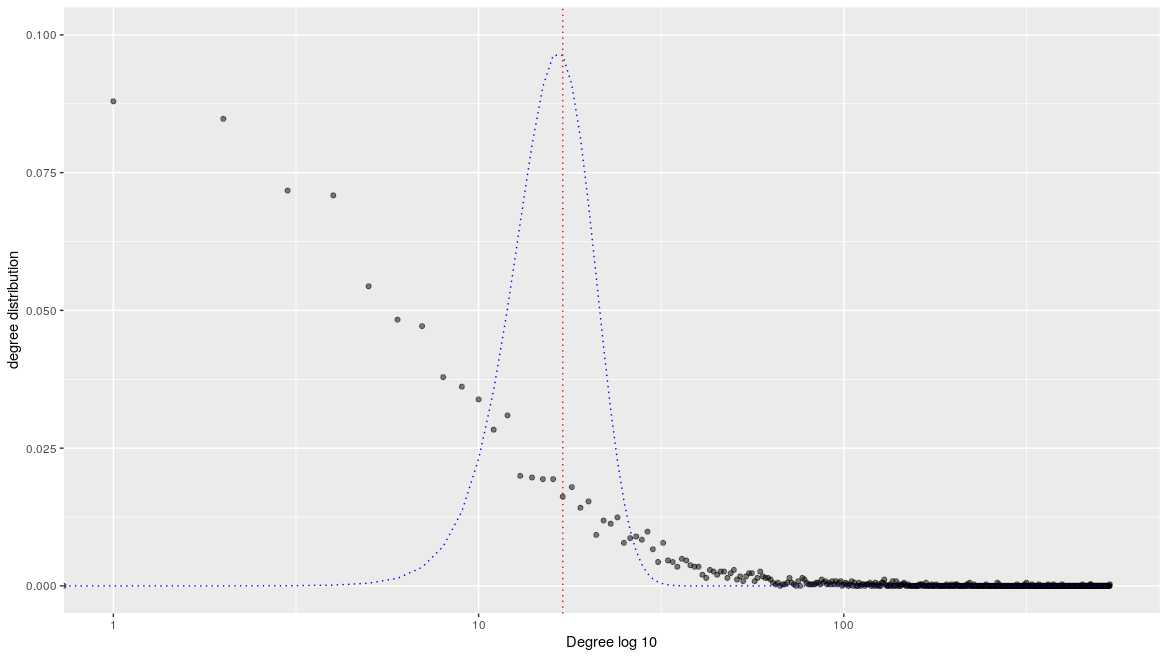
\includegraphics[width=\textwidth]{images/Rplot_poisson_plotted_on_degreedistribution.png}
    \caption{Plot of degree distribution PSP with degree on x axis (log10). Points are degree distribution. Blue dash expected degree distribution given Poisson distribution. Red dash average degree \url{source('~/RProjects/group_size_distribution/R/poissonanddegree.R')}}
    \label{fig:PSP degree powerlaw poisson}
\end{figure}

% \begin{figure}
%   \includegraphics[width=\linewidth]{./dependence_of_scale_coefficient_on_min_degree.png}
%   \caption{The parameter $\gamma$ as a function of the degree at which calculation of the coefficient starts in the degree sequence(e.g. all degree $>5$) from \url{RProjects/PhDGraphs/calculate/gamma}} 
%   \label{fig:gamma}
% \end{figure}

% \begin{figure}
%   \includegraphics[width=\linewidth]{plot_log_degree_distribution.png}
%   \caption{The plot of log cumulative cdf of degree distribution log 10 scale x and y}
%   \label{fig:log_degree_distribution}
% \end{figure}


\begin{figure}
    \centering
    \begin{subfigure}[t]{0.45\textwidth}
        \centering
        \includegraphics[width=\linewidth]{images/dependence_of_scale_coefficient_on_min_degree.png} 
        \caption{The parameter $\gamma$ as a function of the degree at which calculation of the coefficient starts in the degree sequence(e.g. all degree $>5$) from \url{RProjects/PhDGraphs/calculate/gamma}} \label{fig:gamma}
    \end{subfigure}
    \hfill
    \begin{subfigure}[t]{0.45\textwidth}
        \centering
        \includegraphics[width=\linewidth]{images/plot_log_degree_distribution.png} 
        \caption{The plot of log cumulative cdf of degree distribution log 10 scale x and y} \label{fig:log_degree_distribution}
    \end{subfigure}
    \caption{Plots of degree distribution \textcolor{red}{may want to do this in subfigure packages rather than subcaption to line up edges}}
\end{figure}
% latex table generated in R 3.4.4 by xtable 1.8-4 package
% Sat Oct  5 16:31:0\begin{document}

\begin{table}[ht]
\centering
\begin{tabular}{lr}
  \hline
  from degree $k$ & coefficient $\gamma$ \\ 
  \hline
1 & 1.38 \\ 
  5 & 1.81 \\ 
  10 & 2.10 \\ 
  15 & 2.30 \\ 
  20 & 2.43 \\ 
  25 & 2.51 \\ 
   30 & 2.52 \\ 
  35 & 2.54 \\ 
   40 & 2.54 \\ 
   45 & 2.60 \\ 
  50 & 2.63 \\ 
   60 & 2.60 \\ 
   70 & 2.72 \\ 
   80 & 2.80 \\ 
   90 & 2.90 \\ 
   100 & 2.92 \\ 
  150 & 2.88 \\ 
   200 & 3.44 \\ 
   250 & 3.90 \\ 
  300 & 5.04 \\ 
   350 & 5.51 \\ 
   400 & 6.33 \\ 
   \hline
\end{tabular}
\caption{The $\gamma$ as a function of the degree sequence start (e.g. all degree $>5$). from RProjects/PhDGraphs}
  \label{table:gamma}
\end{table}

\subsection{Relationship of C(k) to k}
\todo{add an introduction to this result and significance}
Albert \cite{albert2005scale} says that the relationship C(k) where C(k) is the average transitivity for degree k follows
\begin{equation}
            C(k) = \frac{B}{k^{\beta}}
\end{equation}
\label{eq:C(k) function average transitivity and degree}

citing \cite{yook2004functional} where $\beta$ is between 1 and 2 \cite{albert2005scale}.

When a node has degree 1 the transitivity is  either 0 or undefined so this point has been removed from the plot. 

The graph of degree with log10 scaling and mean transitivity is shown in figure~\ref{fig:C(k)_remove0}

\todo{need to do fit}
\todo{significance of result}
Code \url{source('~/RProjects/graph2community/R/transitivity_degree/Cluster_nodes.R')}
? fit with no intercept

Fitting a linear model omitting degree 1 and with log10 degree has Adjusted R-squared 0.61 compared to 0.4594 for the non logarithmic model.

\textcolor{red}{Actually the first three points have high leverage for this perhaps should try the powerlaw x min but is not a distribution}

R sq 0.65 going from degree 5 so not too much different

\begin{figure}
    \centering
    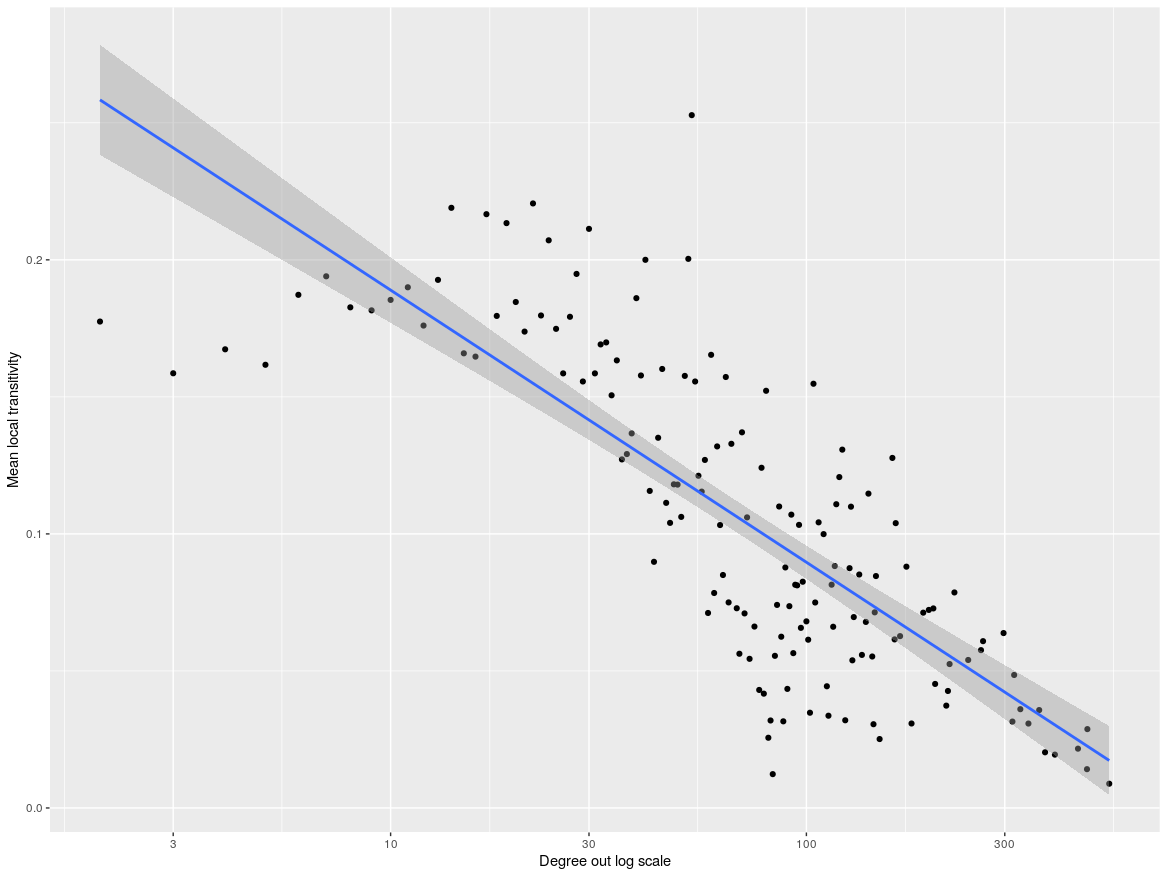
\includegraphics[width=\textwidth]{images/Rplot_k(c)_remove0.png}
    \caption{Plot of degree $k$ log 10 scale with $C(k)$ where $C(k)$ is the mean local undirected transitivity at degree $k$. The point of degree 1 has been removed from the plot and the linear fit as by definition C(k) is 0 as all nodes of degree 1 have local tranisitivity 0 or it is not defined (ie they are isolates)}
    \label{fig:C(k)_remove0}
\end{figure}
\section{ Results Average path length}
\label{sec:Results average path length and transitivity}
The average path length calculated using the \texttt{mean\_distance} function in igraph is 2.98. Global (not WS) transitivity 0.0697.

Average path length for an Erdos Renyi graph on 1000 iterations (type gnm) 3.118 sd 0.00048

Mean global transitivity PSP Watts and Strogatz, isolates to 0 = 0.156. If setting isolates to NA and removing NA = 0.1713.

ER Mean global transititivity (Watts and Strogatz, isolates to 0) 0.0051

ER mean global transitivity (Watts and strogatz, isolates NA and remove 0.0051 (not identical isolates to 0 0.005098806, na 0.005116117)

ER mean global transitivity (triangles 0.005100209 \todo{change to correct sf but keep for now for check not using equal values}) sd 0.0001625842

% latex table generated in R 3.6.3 by xtable 1.8-4 package
% Sat Jun 20 16:17:24 2020
\begin{table}[ht]
\centering
\begin{tabular}{rlrrr}
  \hline
 & variable & mean & sd & PSP \\ 
  \hline
1 & mean\_dist & 3.1182075093 & 0.0004731233 & 2.9797920751 \\ 
  2 & global\_transitivity & 0.0051154572 & 0.0001546763 & 0.0697271768 \\ 
  3 & global\_transitivity\_ws & 0.0051243477 & 0.0001684787 & 0.1562997932 \\ 
  4 & global\_transitivity\_wsNA & 0.0051243477 & 0.0001684787 & 0.1713696115 \\ 
   \hline
\end{tabular}
\caption{Supplemental 10 sf to show that the values are not identical Erdos renyi n3457 m 30498 graph}
\label{tab:transitivity_erdos_renyi 10sf}
\end{table}
% latex table generated in R 3.6.3 by xtable 1.8-4 package
% Sat Jun 20 16:07:46 2020

% latex table generated in R 3.6.3 by xtable 1.8-4 package
% Sat Jun 20 16:19:29 2020
\begin{table}[ht]
\centering
\begin{tabular}{rlrrr}
  \hline
 & variable & mean & sd & PSP \\ 
  \hline
1 & mean\_dist & 3.1182 & 0.0005 & 2.9798 \\ 
  2 & global\_transitivity & 0.0051 & 0.0002 & 0.0697 \\ 
  3 & global\_transitivity\_ws & 0.0051 & 0.0002 & 0.1563 \\ 
  4 & global\_transitivity\_wsNA & 0.0051 & 0.0002 & 0.1714 \\ 
   \hline
\end{tabular}
\caption{Erdos renyi n3457 m 30498 graph}
\label{tab:transitivity_erdos_renyi}
\end{table}

See table~\ref{tab:transitivity_erdos_renyi}
Code \url{source('~/RProjects/graph_sw/R/small_world_random/er_random_ws.R')}

For the degree corrected configuration model see table~\ref{tab:cmtransitivity_configuration_model}. The average path length is shorter than in the Erdos Renyi model likely due to the presence of hub nodes. Code \url{source('~/RProjects/graph_sw/R/small_world_random/degree_corrected_config_random_ws.R')}

% Sat Jun 20 16:38:56 2020
\begin{table}[ht]
\centering
\begin{tabular}{rlrrr}
  \hline
 & variable & mean & sd & PSP \\ 
  \hline
1 & mean\_dist & 3.0069 & 0.0053 & 2.9798 \\ 
  2 & global\_transitivity & 0.0584 & 0.0008 & 0.0697 \\ 
  3 & global\_transitivity\_ws & 0.0683 & 0.0019 & 0.1563 \\ 
  4 & global\_transitivity\_wsNA & 0.0748 & 0.0020 & 0.1714 \\ 
   \hline
\end{tabular}
\caption{Degree corrected configuration model transitivity and average path length. The average path length is smaller than in the Erdos Renyi model likely due to the increased number of hubs}
\label{tab:cmtransitivity_configuration_model}
\end{table}
This is similar to the L of 2.65 and C of 0.28 of C elegans \todo{reference and what is l and c I think c is clustering coefficient}. The random rewiring with a uniform probability leads to a L of 3.11. \todo{add table of path length} See table~\ref{tab:clustering and path length Watts and Strogatz}


\begin{table}[h]
    \centering
    \begin{tabular}{lllll}
    Network      & L\textsubscript{actual} & L\textsubscript{random} & C\textsubscript{actual} & C\textsubscript{random} \\
    \hline
     Film actors    & 3.65 & 2.99 & 0.79 & 0.00027\\
     Power grid & 18.7 & 12.4 & 0.080 & 0.005 \\
     \textit{C elegans} & 2.65 & 2.25 & 0.28 & 0.05 \\
    \end{tabular}
    \caption{Clustering coefficient and average path length from Watts and Strogatz}
    \label{tab:clustering and path length Watts and Strogatz}
\end{table}

\todo{add omnigenic bit}%see code source('~/RProjects/graph_transitivity/R/transitivity.R')

If we simulate mean distance using a degree sequence model we get no distance $<$ empirical distance of 2.979 in 1000 simulations.
\subsection{Results The characterisation of high degree nodes}
The first question we must ask of high degree nodes what are they. Is there something it is like to be a high degree node so we might expected difference behaviour of the nodes in disorders.
\todo{Do we therefore do this for all centrality measures or remove it or just degree}
Are nodes of high degree different to the rest of the PSP in terms of function. 
\textcolor{red}{Why are you telling me this that there is something it is like to be a high degree node so we might expect different enrichment in disease. I think it is high degree nodes are different from a random sampling of the PSP however they do not affect this specific phenotype the literature on centralities is contradictory and has to go piece by piece and with best evidence which in this case is tissue specific networks and GWA}

% latex table generated in R 3.6.2 by xtable 1.8-4 package
% Sat Jan  4 12:23:24 2020
\begin{table}[ht]
\centering
\scalebox{0.8}{
\begin{tabular}{rrll}
  \hline
Entrez & Degree & Symbol & Description \\ 
\hline
351 & 535 & APP & amyloid beta precursor protein \\ 
  2335 & 474 & FN1 & fibronectin 1\footnote{Fibronectin lethality} \\ 
  1994 & 473 & ELAVL1 & ELAV like RNA binding protein 1 \\ 
  1956 & 450 & EGFR & epidermal growth factor receptor \\ 
  7514 & 396 & XPO1 & exportin 1 \\ 
  10482 & 375 & NXF1 & nuclear RNA export factor 1 \\ 
  7316 & 363 & UBC & ubiquitin C \\ 
  26270 & 342 & FBXO6 & F-box protein 6 \\ 
  7412 & 327 & VCAM1 & vascular cell adhesion molecule 1 \\ 
  55832 & 316 & CAND1 & cullin associated and neddylation dissociated 1 \\ 
  8454 & 316 & CUL1 & cullin 1 \\ 
  2885 & 313 & GRB2 & growth factor receptor bound protein 2 \\ 
  7534 & 298 & YWHAZ & tyrosine 3-monooxygenase tryptophan 5-monooxygenase \\
  3320 & 266 & HSP90AA1 & heat shock protein 90 alpha family class A member 1 \\ 
  10075 & 263 & HUWE1 & HECT, UBA and WWE domain containing 1, E3 ubiquitin protein ligase \\ 
  4869 & 263 & NPM1 & nucleophosmin 1 \\ 
  7415 & 245 & VCP & valosin containing protein \\ 
  3178 & 227 & HNRNPA1 & heterogeneous nuclear ribonucleoprotein A1 \\ 
  22938 & 221 & SNW1 & SNW domain containing 1 \\ 
  8453 & 221 & CUL2 & cullin 2 \\ 
   \hline
\end{tabular}
}
\caption{The 20 post synaptic proteome genes with highest degree in their cognate proteins.NOTE tablewidthmodifiedusingscalebox. Code to generate table at \url{source('~/RProjects/gridsearch_gamma/R/degree_distribution.R')}}  
\label{Table:The 20 post synaptic proteome genes with highest degree in their cognate proteins.}
\end{table}
Table \ref{Table:The 20 post synaptic proteome genes with highest degree in their cognate proteins.} shows the 20 post synaptic proteome genes with highest degree and their associated degree. 7 of these genes are part of the ubiquitin protein binding process. \todo{Add class analysis panther}


\begin{figure}
    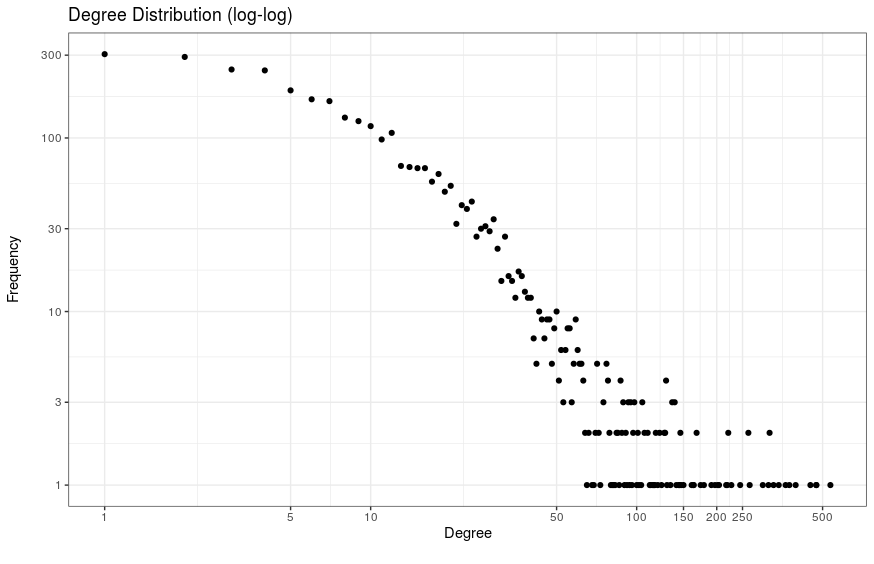
\includegraphics[width=12cm]{Rplot_DegreeDistribution}
    \caption{Degree distribution of post synaptic proteome. Log10 - log10 scale. Code at \url{source('~/RProjects/gridsearch_gamma/R/plot_log_degreedist.R') }}
    \label{fig:Degree distribution of post synaptic proteome. Log10 - log10 scale.}
\end{figure}

\subsection{Degree and Gene Ontology enrichment}

Using the 95th centile of degree distribution (59) we obtained 165 genes. Gene ontology enrichment analysis shows that they are over represented compared with the rest of the proteome for tau protein binding, ubiquitin pathways and cadherin binding.

\subsection{Enrichment compared to PSP}

Using SLIM ontology enrichment was found compared to the rest of the PSP for the biological process (table~\ref{tab:GO SLIM ontology enrichment Biological Process background PSP})

\begin{table}
\centering
\begin{adjustbox}{max width=\textwidth}
\begin{tabular}{llllllllll}
Name & Ontology ref &ref &	expected &	Fold Enrichment &	+/-	&raw P value&FDR\\
\hline
ubiquitin protein ligase & GO:0031625&  	7 &  	.74 & 	9.48 &  	+ & 	$5.08\times 10^{-05}$ & 	$2.43 \times 10^{-02}$\\
\end{tabular}
\end{adjustbox}
\caption{GO SLIM ontology enrichment Biological Process background PSP \textcolor{red}{PUT THESE ALL INTO ONE TABLE}}
\label{tab:GO SLIM ontology enrichment Biological Process background PSP}
\end{table}



SLIM Biological process was enriched for ubiquitin protein ligase (table~\ref{tab:GO SLIM ontology Table:Test for normality (Shapiro-Wilk) for centrality measures of PSPenrichment Biological Process background PSP})% latex table generated in R 3.6.3 by xtable 1.8-4 package
% Tue Jun  2 15:25:40 2020






\todo{redo some of these to check}
\begin{table}
\centering
\begin{adjustbox}{max width=\textwidth}
\begin{tabular}{l l l l l l l l l l}
Name & Ontologyref &ref & set&	expected &	Fold Enrichment &	+/-	&raw P value&FDR\\
\hline
proteasome-mediated ubiquitin-dependent &GO:0043161 & 48 & 	12  &	2.73 &	4.40 & 	+ & 	6.27E-05 & 	4.98E-02 \\
protein catabolic process\\
cell cycle& GO:0007049&	175 	&26 &	9.94& 	2.61 &	+ & 	3.29E-05& 5.22E-02\\
\end{tabular}
\end{adjustbox}
\caption{GO SLIM Biological process High degree nodes}
\label{tab: high degree slim biological process}
\end{table}

\subsubsection{Cellular compartment GO SLIM}
GO SLIM cellular compartment revealed enrichment for intra-nuclear organelles (table~\ref{tab: high degree slim cellular compartment}).

\begin{table}
\centering
\begin{adjustbox}{max width=\textwidth}
\begin{tabular}{llllllll}
  Name  &ref &set &	expected &	Fold Enrichment &	+/-	&raw P value&FDR\\
\hline
nucleus &	459& 	50& 	26.08& 	1.92& 	+ &	$1.60\times 10^{-05}$& 	$6.67\times 10^{-03}$\\
intracellular membrane-bounded organelle&	489&	51&	27.79&	1.84&	+&	$4.21\times10^{-05}$ &	$8.78\times 10^{-03}$\\
intracellular organelle&	490&	51&	27.84&	1.83&	+&	$4.31\times 10^{-05}$&	$5.98\times10^{-03}$\\
\end{tabular}
\end{adjustbox}
\caption{High degree GO SLIM cellular compartment}
\label{tab: high degree slim cellular compartment}
\end{table}

\subsubsection{Molecular function full}
Ontology enrichment of the full molecular
 function revealed enrichment of the WNT signolosome too
\begin{table}
\centering
\begin{adjustbox}{max width=\textwidth}
\begin{tabular}{l l l l l l l l}
Name  &ref & set&	expected &	Fold Enrichment &	+/-	&rawPvalue&FDR\\
\hline
Wnt signalosome& 	7& 	5& 	.40& 	12.57&	+ &	$2.51\time10^{-04}$& 	$8.15\times10^{-03}$\\ 
\end{tabular}
\end{adjustbox}
\caption{Molecular function. Full set ie not go slim ? PSP}
\label{tab:Molecular function. Full set ie not go slim ? PSP}
\end{table}

5 of the 7 elements of the signalosome are in the core segment and there are only 12 in the genome altogether.

\subsection{GO SLIM enrichment against all genome} 

\subsubsection{Cellular compartment }
See table~\ref{tab:Cellular component high degree GO SLIM against genome}
\begin{table}
\centering
\begin{adjustbox}{max width=\textwidth}
\begin{tabular}{lllllllll}
  Name & GO&	Homo sapiens &ref &	expected &	Fold Enrichment &	+/-	&raw P value&FDR\\
  COP9 signalosome&GO:0008180&	13&	3&	.16&	18.35&	+&	9.41E-04&	2.81E-02\\
  microtubule cytoskeleton &GO:0015630&	335&	13&	4.21&	3.09&	+&	4.40E-04&	1.64E-02\\
\end{tabular}
\end{adjustbox}
\caption{Cellular component high degree GO SLIM against genome}
\label{tab:Cellular component high degree GO SLIM against genome}
\end{table}

\subsubsection{Molecular function}
See table~\ref{tab:Molecular function high degree GO SLIM against genome} 
\begin{table}
\centering
\begin{adjustbox}{max width=\textwidth}
\begin{tabular}{lllllllll}
  Name & GO&	Homo sapiens &ref &	expected &	Fold Enrichment &	+/-	&rawPvalue&FDR\\
\hline
ubiquitin protein ligase binding&GO:0031625&	34&	7&	.43&	16.37&	+&	6.59E-07&	1.66E-04\\
\end{tabular}
\end{adjustbox}
\caption{Molecular function high degree GO SLIM against genome}
\label{tab:Molecular function high degree GO SLIM against genome}
\end{table}

\subsubsection{Biological process}
Biological process bit of mixed bag nothing interesting 

\footnote{text files in \url{/home/grant/RProjects/gridsearch_gamma}}

\section{Gene ontology R topgo}
\cite{alexa2009gene}
\subsection{Degree}

% latex table generated in R 3.6.3 by xtable 1.8-4 package
% Sat Jun 13 17:17:49 2020
\begin{table}[ht]
\centering
\begin{adjustbox}{max width=\textwidth}
\begin{tabular}{llrrrrr}
  \hline
GO.ID & Term & Annotated & Significant & Expected & classic & fdr \\ 
  \hline
GO:0051641 & cellular localization & 1575 & 158 & 59.0 & $1.000 \times 10^{-30}$ & $6.683 \times 10^{-28}$ \\ 
  GO:0051128 & regulation of cellular component organiz... & 1458 & 149 & 54.6 & $1.000 \times 10^{-30}$ & $6.683 \times 10^{-28}$ \\ 
  GO:0006996 & organelle organization & 1932 & 172 & 72.4 & $1.000 \times 10^{-30}$ & $6.683 \times 10^{-28}$ \\ 
  GO:0009057 & macromolecule catabolic process & 761 & 106 & 28.5 & $1.000 \times 10^{-30}$ & $6.683 \times 10^{-28}$ \\ 
  GO:0071840 & cellular component organization or bioge... & 3460 & 231 & 129.6 & $1.000 \times 10^{-30}$ & $6.683 \times 10^{-28}$ \\ 
  GO:0044265 & cellular macromolecule catabolic process & 601 & 92 & 22.5 & $1.000 \times 10^{-30}$ & $6.683 \times 10^{-28}$ \\ 
  GO:0044403 & symbiont process & 660 & 95 & 24.7 & $1.000 \times 10^{-30}$ & $6.683 \times 10^{-28}$ \\ 
  GO:0016043 & cellular component organization & 3393 & 225 & 127.1 & $1.000 \times 10^{-30}$ & $6.683 \times 10^{-28}$ \\ 
  GO:0044085 & cellular component biogenesis & 1776 & 158 & 66.5 & $1.000 \times 10^{-30}$ & $6.683 \times 10^{-28}$ \\ 
  GO:0070727 & cellular macromolecule localization & 1012 & 116 & 37.9 & $1.000 \times 10^{-30}$ & $6.683 \times 10^{-28}$ \\ 
  GO:0044419 & interspecies interaction between organis... & 688 & 95 & 25.8 & $1.000 \times 10^{-30}$ & $6.683 \times 10^{-28}$ \\ 
  GO:0016032 & viral process & 621 & 90 & 23.3 & $1.000 \times 10^{-30}$ & $6.683 \times 10^{-28}$ \\ 
  GO:0034613 & cellular protein localization & 1007 & 115 & 37.7 & $1.000 \times 10^{-30}$ & $6.683 \times 10^{-28}$ \\ 
  GO:0009894 & regulation of catabolic process & 579 & 86 & 21.7 & $1.000 \times 10^{-30}$ & $6.683 \times 10^{-28}$ \\ 
  GO:0022607 & cellular component assembly & 1687 & 151 & 63.2 & $1.000 \times 10^{-30}$ & $6.683 \times 10^{-28}$ \\ 
  GO:0007049 & cell cycle & 1020 & 115 & 38.2 & $1.000 \times 10^{-30}$ & $6.683 \times 10^{-28}$ \\ 
  GO:0051130 & positive regulation of cellular componen... & 793 & 100 & 29.7 & $2.800 \times 10^{-30}$ & $1.761 \times 10^{-27}$ \\ 
  GO:0008104 & protein localization & 1475 & 136 & 55.3 & $3.400 \times 10^{-28}$ & $2.020 \times 10^{-25}$ \\ 
  GO:0031329 & regulation of cellular catabolic process & 518 & 77 & 19.4 & $1.900 \times 10^{-27}$ & $1.069 \times 10^{-24}$ \\ 
  GO:0033365 & protein localization to organelle & 520 & 77 & 19.5 & $2.400 \times 10^{-27}$ & $1.283 \times 10^{-24}$ \\ 
   \hline
\end{tabular}
\end{adjustbox}
\caption{Gene Ontology Enrichment BP Degree  greater than or equal to0.9 centile.   Value=37 Universe = 3457} 
\label{tab:Gene Ontology Enrichment BP Degree  greater than or equal to0.9 centile.   Value=37 Universe = 3457}
\end{table}

% latex table generated in R 3.6.3 by xtable 1.8-4 package
% Sat Jun 13 17:19:03 2020
\begin{table}[ht]
\centering
\begin{adjustbox}{max width=\textwidth}
\begin{tabular}{llrrrrr}
  \hline
GO.ID & Term & Annotated & Significant & Expected & classic & fdr \\ 
  \hline
GO:0034220 & ion transmembrane transport & 684 & 54 & 22.9 & $1.200 \times 10^{-9}$ & $1.283 \times 10^{-5}$ \\ 
  GO:0006811 & ion transport & 1005 & 68 & 33.6 & $3.900 \times 10^{-9}$ & $2.085 \times 10^{-5}$ \\ 
  GO:0099537 & trans-synaptic signaling & 494 & 42 & 16.5 & $1.400 \times 10^{-8}$ & $4.544 \times 10^{-5}$ \\ 
  GO:0099536 & synaptic signaling & 498 & 42 & 16.7 & $1.700 \times 10^{-8}$ & $4.544 \times 10^{-5}$ \\ 
  GO:0055085 & transmembrane transport & 908 & 61 & 30.4 & $4.200 \times 10^{-8}$ & $8.732 \times 10^{-5}$ \\ 
  GO:0098660 & inorganic ion transmembrane transport & 497 & 41 & 16.6 & $4.900 \times 10^{-8}$ & $8.732 \times 10^{-5}$ \\ 
  GO:0098655 & cation transmembrane transport & 503 & 41 & 16.8 & $6.900 \times 10^{-8}$ & $9.860 \times 10^{-5}$ \\ 
  GO:0007268 & chemical synaptic transmission & 487 & 40 & 16.3 & $8.300 \times 10^{-8}$ & $9.860 \times 10^{-5}$ \\ 
  GO:0098916 & anterograde trans-synaptic signaling & 487 & 40 & 16.3 & $8.300 \times 10^{-8}$ & $9.860 \times 10^{-5}$ \\ 
  GO:0098662 & inorganic cation transmembrane transport & 444 & 37 & 14.8 & $1.900 \times 10^{-7}$ & $2.031 \times 10^{-4}$ \\ 
  GO:0006812 & cation transport & 704 & 48 & 23.6 & $1.100 \times 10^{-6}$ & $1.069 \times 10^{-3}$ \\ 
  GO:0030001 & metal ion transport & 542 & 39 & 18.1 & $3.600 \times 10^{-6}$ & $3.043 \times 10^{-3}$ \\ 
  GO:0050808 & synapse organization & 254 & 24 & 8.5 & $3.700 \times 10^{-6}$ & $3.043 \times 10^{-3}$ \\ 
  GO:0036109 & alpha-linolenic acid metabolic process & 9 & 5 & 0.3 & $4.500 \times 10^{-6}$ & $3.437 \times 10^{-3}$ \\ 
  GO:0050804 & modulation of chemical synaptic transmis... & 314 & 26 & 10.5 & $1.600 \times 10^{-5}$ & $1.136 \times 10^{-2}$ \\ 
  GO:0099177 & regulation of trans-synaptic signaling & 315 & 26 & 10.5 & $1.700 \times 10^{-5}$ & $1.136 \times 10^{-2}$ \\ 
  GO:0035637 & multicellular organismal signaling & 159 & 17 & 5.3 & $2.100 \times 10^{-5}$ & $1.230 \times 10^{-2}$ \\ 
  GO:0016054 & organic acid catabolic process & 176 & 18 & 5.9 & $2.200 \times 10^{-5}$ & $1.230 \times 10^{-2}$ \\ 
  GO:0046395 & carboxylic acid catabolic process & 176 & 18 & 5.9 & $2.200 \times 10^{-5}$ & $1.230 \times 10^{-2}$ \\ 
  GO:0009187 & cyclic nucleotide metabolic process & 37 & 8 & 1.2 & $2.300 \times 10^{-5}$ & $1.230 \times 10^{-2}$ \\ 
   \hline
\end{tabular}
\end{adjustbox}
\caption{Gene Ontology Enrichment BP Degree  less than or equal to0.1centile.   Value=2 Universe = 3457} 
\label{tab:Gene Ontology Enrichment BP Degree  less than or equal to0.1centile.   Value=2 Universe = 3457}
\end{table}

\subsection{Degree Molecular Function}
% latex table generated in R 3.6.3 by xtable 1.8-4 package
% Sat Jun 13 17:20:59 2020
\begin{table}[ht]
\centering
\begin{adjustbox}{max width=\textwidth}
\begin{tabular}{llrrrrr}
  \hline
GO.ID & Term & Annotated & Significant & Expected & classic & fdr \\ 
  \hline
GO:0003723 & RNA binding & 827 & 110 & 31.4 & $1.000 \times 10^{-30}$ & $1.960 \times 10^{-27}$ \\ 
  GO:0019899 & enzyme binding & 1343 & 141 & 51.0 & $1.000 \times 10^{-30}$ & $1.960 \times 10^{-27}$ \\ 
  GO:0005515 & protein binding & 5964 & 285 & 226.3 & $4.800 \times 10^{-25}$ & $5.585 \times 10^{-22}$ \\ 
  GO:0019904 & protein domain specific binding & 489 & 72 & 18.6 & $5.700 \times 10^{-25}$ & $5.585 \times 10^{-22}$ \\ 
  GO:0045296 & cadherin binding & 238 & 49 & 9.0 & $2.100 \times 10^{-23}$ & $1.646 \times 10^{-20}$ \\ 
  GO:0050839 & cell adhesion molecule binding & 377 & 59 & 14.3 & $1.000 \times 10^{-21}$ & $6.532 \times 10^{-19}$ \\ 
  GO:0031625 & ubiquitin protein ligase binding & 208 & 43 & 7.9 & $1.200 \times 10^{-20}$ & $6.368 \times 10^{-18}$ \\ 
  GO:0044389 & ubiquitin-like protein ligase binding & 219 & 44 & 8.3 & $1.300 \times 10^{-20}$ & $6.368 \times 10^{-18}$ \\ 
  GO:0044877 & protein-containing complex binding & 782 & 85 & 29.7 & $1.900 \times 10^{-20}$ & $8.273 \times 10^{-18}$ \\ 
  GO:1901363 & heterocyclic compound binding & 3074 & 191 & 116.7 & $2.400 \times 10^{-19}$ & $9.263 \times 10^{-17}$ \\ 
  GO:0097159 & organic cyclic compound binding & 3128 & 193 & 118.7 & $2.600 \times 10^{-19}$ & $9.263 \times 10^{-17}$ \\ 
  GO:0019900 & kinase binding & 507 & 63 & 19.2 & $7.600 \times 10^{-18}$ & $2.482 \times 10^{-15}$ \\ 
  GO:0017076 & purine nucleotide binding & 1097 & 98 & 41.6 & $1.300 \times 10^{-17}$ & $3.919 \times 10^{-15}$ \\ 
  GO:0035639 & purine ribonucleoside triphosphate bindi... & 1047 & 95 & 39.7 & $1.800 \times 10^{-17}$ & $5.039 \times 10^{-15}$ \\ 
  GO:0019901 & protein kinase binding & 456 & 58 & 17.3 & $6.700 \times 10^{-17}$ & $1.750 \times 10^{-14}$ \\ 
  GO:0032555 & purine ribonucleotide binding & 1088 & 96 & 41.3 & $7.800 \times 10^{-17}$ & $1.911 \times 10^{-14}$ \\ 
  GO:0032553 & ribonucleotide binding & 1096 & 96 & 41.6 & $1.300 \times 10^{-16}$ & $2.997 \times 10^{-14}$ \\ 
  GO:0030554 & adenyl nucleotide binding & 928 & 85 & 35.2 & $1.000 \times 10^{-15}$ & $2.177 \times 10^{-13}$ \\ 
  GO:0000166 & nucleotide binding & 1234 & 101 & 46.8 & $1.600 \times 10^{-15}$ & $3.300 \times 10^{-13}$ \\ 
  GO:1901265 & nucleoside phosphate binding & 1235 & 101 & 46.9 & $1.700 \times 10^{-15}$ & $3.331 \times 10^{-13}$ \\ 
   \hline
\end{tabular}
\end{adjustbox}
\caption{Gene Ontology Enrichment MF Degree  greater than or equal to0.9 centile.   Value=37 Universe = 3457} 
\label{tab:Gene Ontology Enrichment MF Degree  greater than or equal to0.9 centile.   Value=37 Universe = 3457}
\end{table}

% latex table generated in R 3.6.3 by xtable 1.8-4 package
% Sat Jun 13 17:21:32 2020
\begin{table}[ht]
\centering
\begin{adjustbox}{max width=\textwidth}
\begin{tabular}{llrrrrr}
  \hline
GO.ID & Term & Annotated & Significant & Expected & classic & fdr \\ 
  \hline
GO:0046873 & metal ion transmembrane transporter acti... & 255 & 35 & 8.3 & $2.400 \times 10^{-13}$ & $9.210 \times 10^{-10}$ \\ 
  GO:0022857 & transmembrane transporter activity & 557 & 53 & 18.1 & $4.700 \times 10^{-13}$ & $9.210 \times 10^{-10}$ \\ 
  GO:0015075 & ion transmembrane transporter activity & 485 & 48 & 15.8 & $1.700 \times 10^{-12}$ & $2.221 \times 10^{-9}$ \\ 
  GO:0008324 & cation transmembrane transporter activit... & 369 & 41 & 12.0 & $2.300 \times 10^{-12}$ & $2.253 \times 10^{-9}$ \\ 
  GO:0005215 & transporter activity & 604 & 54 & 19.7 & $3.300 \times 10^{-12}$ & $2.587 \times 10^{-9}$ \\ 
  GO:0015318 & inorganic molecular entity transmembrane... & 465 & 46 & 15.2 & $5.600 \times 10^{-12}$ & $3.658 \times 10^{-9}$ \\ 
  GO:0022890 & inorganic cation transmembrane transport... & 349 & 39 & 11.4 & $7.000 \times 10^{-12}$ & $3.919 \times 10^{-9}$ \\ 
  GO:0005244 & voltage-gated ion channel activity & 127 & 20 & 4.1 & $3.800 \times 10^{-9}$ & $1.655 \times 10^{-6}$ \\ 
  GO:0022832 & voltage-gated channel activity & 127 & 20 & 4.1 & $3.800 \times 10^{-9}$ & $1.655 \times 10^{-6}$ \\ 
  GO:0022838 & substrate-specific channel activity & 253 & 28 & 8.2 & $1.100 \times 10^{-8}$ & $4.311 \times 10^{-6}$ \\ 
  GO:0005216 & ion channel activity & 242 & 27 & 7.9 & $1.700 \times 10^{-8}$ & $6.057 \times 10^{-6}$ \\ 
  GO:0015267 & channel activity & 266 & 28 & 8.7 & $3.200 \times 10^{-8}$ & $9.518 \times 10^{-6}$ \\ 
  GO:0022803 & passive transmembrane transporter activi... & 266 & 28 & 8.7 & $3.200 \times 10^{-8}$ & $9.518 \times 10^{-6}$ \\ 
  GO:0022839 & ion gated channel activity & 218 & 25 & 7.1 & $3.400 \times 10^{-8}$ & $9.518 \times 10^{-6}$ \\ 
  GO:0022836 & gated channel activity & 220 & 25 & 7.2 & $4.100 \times 10^{-8}$ & $1.071 \times 10^{-5}$ \\ 
  GO:0005261 & cation channel activity & 191 & 23 & 6.2 & $4.900 \times 10^{-8}$ & $1.200 \times 10^{-5}$ \\ 
  GO:0015077 & monovalent inorganic cation transmembran... & 240 & 25 & 7.8 & $2.300 \times 10^{-7}$ & $5.302 \times 10^{-5}$ \\ 
  GO:0022843 & voltage-gated cation channel activity & 95 & 15 & 3.1 & $3.500 \times 10^{-7}$ & $7.620 \times 10^{-5}$ \\ 
  GO:0005245 & voltage-gated calcium channel activity & 31 & 9 & 1.0 & $3.900 \times 10^{-7}$ & $8.044 \times 10^{-5}$ \\ 
  GO:0015081 & sodium ion transmembrane transporter act... & 102 & 14 & 3.3 & $4.900 \times 10^{-6}$ & $9.602 \times 10^{-4}$ \\ 
   \hline
\end{tabular}
\end{adjustbox}
\caption{Gene Ontology Enrichment MF Degree  less than or equal to0.1centile.   Value=2 Universe = 3457} 
\label{tab:Gene Ontology Enrichment MF Degree  less than or equal to0.1centile.   Value=2 Universe = 3457}
\end{table}


\subsection{Degree Cellular Component}

% latex table generated in R 3.6.3 by xtable 1.8-4 package
% Sat Jun 13 17:22:14 2020
\begin{table}[ht]
\centering
\begin{adjustbox}{max width=\textwidth}
\begin{tabular}{llrrrrr}
  \hline
GO.ID & Term & Annotated & Significant & Expected & classic & fdr \\ 
  \hline
GO:0005829 & cytosol & 2768 & 222 & 103.2 & $1.000 \times 10^{-30}$ & $2.071 \times 10^{-28}$ \\ 
  GO:0043228 & non-membrane-bounded organelle & 2071 & 190 & 77.2 & $1.000 \times 10^{-30}$ & $2.071 \times 10^{-28}$ \\ 
  GO:0043232 & intracellular non-membrane-bounded organ... & 2064 & 189 & 77.0 & $1.000 \times 10^{-30}$ & $2.071 \times 10^{-28}$ \\ 
  GO:0032991 & protein-containing complex & 2970 & 216 & 110.8 & $1.000 \times 10^{-30}$ & $2.071 \times 10^{-28}$ \\ 
  GO:0044446 & intracellular organelle part & 4590 & 262 & 171.2 & $1.000 \times 10^{-30}$ & $2.071 \times 10^{-28}$ \\ 
  GO:0005856 & cytoskeleton & 1037 & 118 & 38.7 & $1.000 \times 10^{-30}$ & $2.071 \times 10^{-28}$ \\ 
  GO:0044430 & cytoskeletal part & 777 & 101 & 29.0 & $1.000 \times 10^{-30}$ & $2.071 \times 10^{-28}$ \\ 
  GO:0044422 & organelle part & 4733 & 263 & 176.5 & $1.000 \times 10^{-30}$ & $2.071 \times 10^{-28}$ \\ 
  GO:0005634 & nucleus & 3498 & 225 & 130.5 & $1.000 \times 10^{-30}$ & $2.071 \times 10^{-28}$ \\ 
  GO:0044428 & nuclear part & 2365 & 179 & 88.2 & $3.100 \times 10^{-29}$ & $5.778 \times 10^{-27}$ \\ 
  GO:0070062 & extracellular exosome & 1517 & 139 & 56.6 & $7.000 \times 10^{-29}$ & $1.186 \times 10^{-26}$ \\ 
  GO:1903561 & extracellular vesicle & 1531 & 139 & 57.1 & $1.900 \times 10^{-28}$ & $2.951 \times 10^{-26}$ \\ 
  GO:0043230 & extracellular organelle & 1533 & 139 & 57.2 & $2.200 \times 10^{-28}$ & $3.154 \times 10^{-26}$ \\ 
  GO:0005737 & cytoplasm & 5513 & 277 & 205.6 & $1.300 \times 10^{-27}$ & $1.731 \times 10^{-25}$ \\ 
  GO:0043229 & intracellular organelle & 5825 & 283 & 217.3 & $1.500 \times 10^{-27}$ & $1.864 \times 10^{-25}$ \\ 
  GO:0044444 & cytoplasmic part & 4850 & 261 & 180.9 & $2.100 \times 10^{-27}$ & $2.446 \times 10^{-25}$ \\ 
  GO:0031982 & vesicle & 2388 & 175 & 89.1 & $2.300 \times 10^{-26}$ & $2.522 \times 10^{-24}$ \\ 
  GO:0015630 & microtubule cytoskeleton & 538 & 76 & 20.1 & $1.000 \times 10^{-25}$ & $1.036 \times 10^{-23}$ \\ 
  GO:1990904 & ribonucleoprotein complex & 438 & 67 & 16.3 & $1.500 \times 10^{-24}$ & $1.472 \times 10^{-22}$ \\ 
  GO:0031981 & nuclear lumen & 2197 & 162 & 82.0 & $9.200 \times 10^{-24}$ & $8.574 \times 10^{-22}$ \\ 
   \hline
\end{tabular}
\end{adjustbox}
\caption{Gene Ontology Enrichment CC Degree  greater than or equal to0.9 centile.   Value=37 Universe = 3457} 
\label{tab:Gene Ontology Enrichment CC Degree  greater than or equal to0.9 centile.   Value=37 Universe = 3457}
\end{table}

% latex table generated in R 3.6.3 by xtable 1.8-4 package
% Sat Jun 13 17:23:57 2020
\begin{table}[ht]
\centering
\begin{adjustbox}{max width=\textwidth}
\begin{tabular}{llrrrrr}
  \hline
GO.ID & Term & Annotated & Significant & Expected & classic & fdr \\ 
  \hline
GO:0097458 & neuron part & 1089 & 78 & 36.1 & $6.200 \times 10^{-12}$ & $1.156 \times 10^{-8}$ \\ 
  GO:0045202 & synapse & 786 & 62 & 26.1 & $3.500 \times 10^{-11}$ & $3.262 \times 10^{-8}$ \\ 
  GO:1902495 & transmembrane transporter complex & 213 & 28 & 7.1 & $3.100 \times 10^{-10}$ & $1.926 \times 10^{-7}$ \\ 
  GO:1990351 & transporter complex & 216 & 28 & 7.2 & $4.400 \times 10^{-10}$ & $2.050 \times 10^{-7}$ \\ 
  GO:0043005 & neuron projection & 831 & 61 & 27.6 & $1.000 \times 10^{-9}$ & $3.728 \times 10^{-7}$ \\ 
  GO:0034703 & cation channel complex & 147 & 22 & 4.9 & $2.400 \times 10^{-9}$ & $7.456 \times 10^{-7}$ \\ 
  GO:0034702 & ion channel complex & 195 & 25 & 6.5 & $5.000 \times 10^{-9}$ & $1.331 \times 10^{-6}$ \\ 
  GO:0044456 & synapse part & 640 & 50 & 21.2 & $6.100 \times 10^{-9}$ & $1.421 \times 10^{-6}$ \\ 
  GO:0031224 & intrinsic component of membrane & 2187 & 114 & 72.6 & $1.600 \times 10^{-8}$ & $3.314 \times 10^{-6}$ \\ 
  GO:0097060 & synaptic membrane & 276 & 29 & 9.2 & $2.800 \times 10^{-8}$ & $5.219 \times 10^{-6}$ \\ 
  GO:0044425 & membrane part & 2946 & 139 & 97.8 & $8.400 \times 10^{-8}$ & $1.423 \times 10^{-5}$ \\ 
  GO:0016021 & integral component of membrane & 2098 & 108 & 69.6 & $1.100 \times 10^{-7}$ & $1.709 \times 10^{-5}$ \\ 
  GO:0120025 & plasma membrane bounded cell projection & 1160 & 69 & 38.5 & $4.000 \times 10^{-7}$ & $5.735 \times 10^{-5}$ \\ 
  GO:0098978 & glutamatergic synapse & 245 & 25 & 8.1 & $4.800 \times 10^{-7}$ & $6.338 \times 10^{-5}$ \\ 
  GO:0099699 & integral component of synaptic membrane & 109 & 16 & 3.6 & $5.100 \times 10^{-7}$ & $6.338 \times 10^{-5}$ \\ 
  GO:0030424 & axon & 392 & 33 & 13.0 & $6.200 \times 10^{-7}$ & $7.145 \times 10^{-5}$ \\ 
  GO:0044463 & cell projection part & 808 & 53 & 26.8 & $6.900 \times 10^{-7}$ & $7.145 \times 10^{-5}$ \\ 
  GO:0120038 & plasma membrane bounded cell projection ... & 808 & 53 & 26.8 & $6.900 \times 10^{-7}$ & $7.145 \times 10^{-5}$ \\ 
  GO:0099240 & intrinsic component of synaptic membrane & 113 & 16 & 3.8 & $8.400 \times 10^{-7}$ & $8.241 \times 10^{-5}$ \\ 
  GO:0005891 & voltage-gated calcium channel complex & 26 & 8 & 0.9 & $1.200 \times 10^{-6}$ & $1.118 \times 10^{-4}$ \\ 
   \hline
\end{tabular}
\end{adjustbox}
\caption{Gene Ontology Enrichment CC Degree  less than or equal to0.1centile.   Value=2 Universe = 3457} 
\label{tab:Gene Ontology Enrichment CC Degree  less than or equal to0.1centile.   Value=2 Universe = 3457}
\end{table}
\textcolor{red}{move to supplementary tables and described}

\todo{Move to supplementary tables}
\todo{check the fdr are ok ie less than 0.05}

code at \url{source('~/RProjects/centrality/R/go_enrichment/go_enrichment_centrality.R')}
% latex table generated in R 3.6.3 by xtable 1.8-4 package
% Tue Jun  2 14:39:06 2020

\subsection{TopGO Betweenness}

\begin{table}[ht]
\centering
\begin{tabular}{llrrrrr}
  \hline
GO.ID & Term & Annotated & Significant & Expected & classic & fdr \\ 
  \hline
GO:0051641 & cellular localization & 1575 & 159 & 57.6 & $1.000 \times 10^{-30}$ & $1.188 \times 10^{-27}$ \\ 
  GO:0006996 & organelle organization & 1932 & 173 & 70.6 & $1.000 \times 10^{-30}$ & $1.188 \times 10^{-27}$ \\ 
  GO:0071840 & cellular component organization or bioge... & 3460 & 228 & 126.5 & $1.000 \times 10^{-30}$ & $1.188 \times 10^{-27}$ \\ 
  GO:0016043 & cellular component organization & 3393 & 224 & 124.0 & $1.000 \times 10^{-30}$ & $1.188 \times 10^{-27}$ \\ 
  GO:0070727 & cellular macromolecule localization & 1012 & 114 & 37.0 & $1.000 \times 10^{-30}$ & $1.188 \times 10^{-27}$ \\ 
  GO:0044085 & cellular component biogenesis & 1776 & 154 & 64.9 & $1.000 \times 10^{-30}$ & $1.188 \times 10^{-27}$ \\ 
  GO:0034613 & cellular protein localization & 1007 & 113 & 36.8 & $1.000 \times 10^{-30}$ & $1.188 \times 10^{-27}$ \\ 
  GO:0022607 & cellular component assembly & 1687 & 149 & 61.7 & $1.000 \times 10^{-30}$ & $1.188 \times 10^{-27}$ \\ 
  GO:0008104 & protein localization & 1475 & 138 & 53.9 & $1.000 \times 10^{-30}$ & $1.188 \times 10^{-27}$ \\ 
  GO:0033036 & macromolecule localization & 1650 & 145 & 60.3 & $8.900 \times 10^{-30}$ & $9.516 \times 10^{-27}$ \\ 
  GO:0051128 & regulation of cellular component organiz... & 1458 & 135 & 53.3 & $1.800 \times 10^{-29}$ & $1.750 \times 10^{-26}$ \\ 
  GO:0009894 & regulation of catabolic process & 579 & 82 & 21.2 & $1.100 \times 10^{-28}$ & $9.801 \times 10^{-26}$ \\ 
  GO:0009057 & macromolecule catabolic process & 761 & 93 & 27.8 & $9.300 \times 10^{-28}$ & $7.649 \times 10^{-25}$ \\ 
  GO:0060341 & regulation of cellular localization & 580 & 80 & 21.2 & $4.100 \times 10^{-27}$ & $3.131 \times 10^{-24}$ \\ 
  GO:0046907 & intracellular transport & 992 & 106 & 36.3 & $4.600 \times 10^{-27}$ & $3.279 \times 10^{-24}$ \\ 
  GO:0051649 & establishment of localization in cell & 1254 & 120 & 45.8 & $9.700 \times 10^{-27}$ & $6.482 \times 10^{-24}$ \\ 
  GO:1903827 & regulation of cellular protein localizat... & 323 & 58 & 11.8 & $2.400 \times 10^{-25}$ & $1.509 \times 10^{-22}$ \\ 
  GO:0045184 & establishment of protein localization & 1150 & 112 & 42.0 & $2.900 \times 10^{-25}$ & $1.723 \times 10^{-22}$ \\ 
  GO:0031329 & regulation of cellular catabolic process & 518 & 73 & 18.9 & $3.500 \times 10^{-25}$ & $1.970 \times 10^{-22}$ \\ 
  GO:0051130 & positive regulation of cellular componen... & 793 & 90 & 29.0 & $2.300 \times 10^{-24}$ & $1.230 \times 10^{-21}$ \\ 
   \hline
\end{tabular}
\caption{Gene Ontology Enrichment BP Betweenness  greater than or equal to0.9 centile.   Value=5345.16656859608 Universe = 3457} 
\label{tab:Gene Ontology Enrichment BP Betweenness  greater than or equal to0.9 centile.   Value=5345.16656859608 Universe = 3457}
\end{table}

% latex table generated in R 3.6.3 by xtable 1.8-4 package
% Sat Jun 13 17:35:34 2020
\begin{table}[ht]
\centering
\begin{tabular}{llrrrrr}
  \hline
GO.ID & Term & Annotated & Significant & Expected & classic & fdr \\ 
  \hline
GO:0099537 & trans-synaptic signaling & 494 & 28 & 9.3 & $1.000 \times 10^{-7}$ & $6.415 \times 10^{-4}$ \\ 
  GO:0099536 & synaptic signaling & 498 & 28 & 9.4 & $1.200 \times 10^{-7}$ & $6.415 \times 10^{-4}$ \\ 
  GO:0007268 & chemical synaptic transmission & 487 & 26 & 9.2 & $1.000 \times 10^{-6}$ & $2.673 \times 10^{-3}$ \\ 
  GO:0098916 & anterograde trans-synaptic signaling & 487 & 26 & 9.2 & $1.000 \times 10^{-6}$ & $2.673 \times 10^{-3}$ \\ 
  GO:0006811 & ion transport & 1005 & 40 & 18.9 & $1.900 \times 10^{-6}$ & $4.063 \times 10^{-3}$ \\ 
  GO:0034220 & ion transmembrane transport & 684 & 31 & 12.9 & $2.700 \times 10^{-6}$ & $4.811 \times 10^{-3}$ \\ 
  GO:0009187 & cyclic nucleotide metabolic process & 37 & 7 & 0.7 & $4.600 \times 10^{-6}$ & $7.026 \times 10^{-3}$ \\ 
  GO:0050804 & modulation of chemical synaptic transmis... & 314 & 19 & 5.9 & $5.800 \times 10^{-6}$ & $7.247 \times 10^{-3}$ \\ 
  GO:0099177 & regulation of trans-synaptic signaling & 315 & 19 & 5.9 & $6.100 \times 10^{-6}$ & $7.247 \times 10^{-3}$ \\ 
  GO:0055085 & transmembrane transport & 908 & 36 & 17.1 & $8.100 \times 10^{-6}$ & $8.661 \times 10^{-3}$ \\ 
  GO:0009190 & cyclic nucleotide biosynthetic process & 20 & 5 & 0.4 & $2.700 \times 10^{-5}$ & $2.406 \times 10^{-2}$ \\ 
  GO:0052652 & cyclic purine nucleotide metabolic proce... & 20 & 5 & 0.4 & $2.700 \times 10^{-5}$ & $2.406 \times 10^{-2}$ \\ 
  GO:0042391 & regulation of membrane potential & 302 & 17 & 5.7 & $4.700 \times 10^{-5}$ & $3.866 \times 10^{-2}$ \\ 
  GO:0046339 & diacylglycerol metabolic process & 14 & 4 & 0.3 & $1.000 \times 10^{-4}$ & $7.637 \times 10^{-2}$ \\ 
  GO:0098660 & inorganic ion transmembrane transport & 497 & 22 & 9.3 & $1.400 \times 10^{-4}$ & $9.979 \times 10^{-2}$ \\ 
  GO:0090407 & organophosphate biosynthetic process & 413 & 19 & 7.8 & $2.500 \times 10^{-4}$ & $1.671 \times 10^{-1}$ \\ 
  GO:0065008 & regulation of biological quality & 2539 & 68 & 47.7 & $2.900 \times 10^{-4}$ & $1.824 \times 10^{-1}$ \\ 
  GO:0006171 & cAMP biosynthetic process & 8 & 3 & 0.1 & $3.400 \times 10^{-4}$ & $1.970 \times 10^{-1}$ \\ 
  GO:0071926 & endocannabinoid signaling pathway & 2 & 2 & 0.0 & $3.500 \times 10^{-4}$ & $1.970 \times 10^{-1}$ \\ 
  GO:0046058 & cAMP metabolic process & 19 & 4 & 0.4 & $3.700 \times 10^{-4}$ & $1.978 \times 10^{-1}$ \\ 
   \hline
\end{tabular}
\caption{Gene Ontology Enrichment BP Betweenness  less than or equal to0.1centile.   Value=0 Universe = 3457} 
\label{tab:Gene Ontology Enrichment BP Betweenness  less than or equal to0.1centile.   Value=0 Universe = 3457}
\end{table}

Low betweenness centrality and receptors as they are at the end of a pathway so fewer common paths go through

\subsubsection{Betweenness MF}

% latex table generated in R 3.6.3 by xtable 1.8-4 package
% Sat Jun 13 17:37:06 2020
\begin{table}[ht]
\centering
\begin{tabular}{llrrrrr}
  \hline
GO.ID & Term & Annotated & Significant & Expected & classic & fdr \\ 
  \hline
GO:0019899 & enzyme binding & 1343 & 141 & 49.7 & $1.000 \times 10^{-30}$ & $3.919 \times 10^{-27}$ \\ 
  GO:0019904 & protein domain specific binding & 489 & 74 & 18.1 & $3.300 \times 10^{-27}$ & $6.466 \times 10^{-24}$ \\ 
  GO:0005515 & protein binding & 5964 & 278 & 220.9 & $2.600 \times 10^{-24}$ & $3.396 \times 10^{-21}$ \\ 
  GO:0045296 & cadherin binding & 238 & 48 & 8.8 & $5.300 \times 10^{-23}$ & $5.193 \times 10^{-20}$ \\ 
  GO:0050839 & cell adhesion molecule binding & 377 & 59 & 14.0 & $2.800 \times 10^{-22}$ & $2.195 \times 10^{-19}$ \\ 
  GO:0044877 & protein-containing complex binding & 782 & 85 & 29.0 & $3.200 \times 10^{-21}$ & $2.090 \times 10^{-18}$ \\ 
  GO:0008092 & cytoskeletal protein binding & 544 & 67 & 20.1 & $2.100 \times 10^{-19}$ & $1.176 \times 10^{-16}$ \\ 
  GO:0019900 & kinase binding & 507 & 64 & 18.8 & $4.500 \times 10^{-19}$ & $2.204 \times 10^{-16}$ \\ 
  GO:0031625 & ubiquitin protein ligase binding & 208 & 40 & 7.7 & $1.800 \times 10^{-18}$ & $7.446 \times 10^{-16}$ \\ 
  GO:0044389 & ubiquitin-like protein ligase binding & 219 & 41 & 8.1 & $1.900 \times 10^{-18}$ & $7.446 \times 10^{-16}$ \\ 
  GO:0019901 & protein kinase binding & 456 & 57 & 16.9 & $9.100 \times 10^{-17}$ & $3.242 \times 10^{-14}$ \\ 
  GO:0003723 & RNA binding & 827 & 78 & 30.6 & $1.100 \times 10^{-15}$ & $3.592 \times 10^{-13}$ \\ 
  GO:0008022 & protein C-terminus binding & 140 & 27 & 5.2 & $8.600 \times 10^{-13}$ & $2.593 \times 10^{-10}$ \\ 
  GO:0005488 & binding & 6970 & 283 & 258.1 & $2.900 \times 10^{-12}$ & $8.118 \times 10^{-10}$ \\ 
  GO:0042802 & identical protein binding & 1117 & 84 & 41.4 & $2.700 \times 10^{-11}$ & $7.054 \times 10^{-9}$ \\ 
  GO:0017076 & purine nucleotide binding & 1097 & 82 & 40.6 & $7.200 \times 10^{-11}$ & $1.706 \times 10^{-8}$ \\ 
  GO:0044325 & ion channel binding & 91 & 20 & 3.4 & $7.400 \times 10^{-11}$ & $1.706 \times 10^{-8}$ \\ 
  GO:0035639 & purine ribonucleoside triphosphate bindi... & 1047 & 79 & 38.8 & $1.200 \times 10^{-10}$ & $2.475 \times 10^{-8}$ \\ 
  GO:0032555 & purine ribonucleotide binding & 1088 & 81 & 40.3 & $1.200 \times 10^{-10}$ & $2.475 \times 10^{-8}$ \\ 
  GO:0032553 & ribonucleotide binding & 1096 & 81 & 40.6 & $1.800 \times 10^{-10}$ & $3.527 \times 10^{-8}$ \\ 
   \hline
\end{tabular}
\caption{Gene Ontology Enrichment MF Betweenness  greater than or equal to0.9 centile.   Value=5345.16656859608 Universe = 3457} 
\label{tab:Gene Ontology Enrichment MF Betweenness  greater than or equal to0.9 centile.   Value=5345.16656859608 Universe = 3457}
\end{table}

% latex table generated in R 3.6.3 by xtable 1.8-4 package
% Sat Jun 13 17:37:39 2020
\begin{table}[ht]
\centering
\begin{tabular}{llrrrrr}
  \hline
GO.ID & Term & Annotated & Significant & Expected & classic & fdr \\ 
  \hline
GO:0022857 & transmembrane transporter activity & 557 & 30 & 10.2 & $5.500 \times 10^{-8}$ & $1.881 \times 10^{-4}$ \\ 
  GO:0005215 & transporter activity & 604 & 31 & 11.1 & $9.600 \times 10^{-8}$ & $1.881 \times 10^{-4}$ \\ 
  GO:0015075 & ion transmembrane transporter activity & 485 & 27 & 8.9 & $1.500 \times 10^{-7}$ & $1.959 \times 10^{-4}$ \\ 
  GO:0015318 & inorganic molecular entity transmembrane... & 465 & 25 & 8.5 & $9.000 \times 10^{-7}$ & $8.818 \times 10^{-4}$ \\ 
  GO:0008324 & cation transmembrane transporter activit... & 369 & 21 & 6.8 & $3.100 \times 10^{-6}$ & $2.351 \times 10^{-3}$ \\ 
  GO:0046873 & metal ion transmembrane transporter acti... & 255 & 17 & 4.7 & $3.600 \times 10^{-6}$ & $2.351 \times 10^{-3}$ \\ 
  GO:0022890 & inorganic cation transmembrane transport... & 349 & 20 & 6.4 & $4.900 \times 10^{-6}$ & $2.743 \times 10^{-3}$ \\ 
  GO:0009975 & cyclase activity & 18 & 5 & 0.3 & $1.400 \times 10^{-5}$ & $6.858 \times 10^{-3}$ \\ 
  GO:0016849 & phosphorus-oxygen lyase activity & 19 & 5 & 0.3 & $1.800 \times 10^{-5}$ & $7.838 \times 10^{-3}$ \\ 
  GO:0022839 & ion gated channel activity & 218 & 13 & 4.0 & $1.700 \times 10^{-4}$ & $6.662 \times 10^{-2}$ \\ 
  GO:0022836 & gated channel activity & 220 & 13 & 4.0 & $1.900 \times 10^{-4}$ & $6.769 \times 10^{-2}$ \\ 
  GO:0004016 & adenylate cyclase activity & 8 & 3 & 0.1 & $3.200 \times 10^{-4}$ & $1.045 \times 10^{-1}$ \\ 
  GO:0015077 & monovalent inorganic cation transmembran... & 240 & 13 & 4.4 & $4.300 \times 10^{-4}$ & $1.222 \times 10^{-1}$ \\ 
  GO:0005216 & ion channel activity & 242 & 13 & 4.4 & $4.700 \times 10^{-4}$ & $1.222 \times 10^{-1}$ \\ 
  GO:0005244 & voltage-gated ion channel activity & 127 & 9 & 2.3 & $5.100 \times 10^{-4}$ & $1.222 \times 10^{-1}$ \\ 
  GO:0022832 & voltage-gated channel activity & 127 & 9 & 2.3 & $5.100 \times 10^{-4}$ & $1.222 \times 10^{-1}$ \\ 
  GO:0015081 & sodium ion transmembrane transporter act... & 102 & 8 & 1.9 & $5.300 \times 10^{-4}$ & $1.222 \times 10^{-1}$ \\ 
  GO:0022838 & substrate-specific channel activity & 253 & 13 & 4.6 & $7.200 \times 10^{-4}$ & $1.568 \times 10^{-1}$ \\ 
  GO:0008332 & low voltage-gated calcium channel activi... & 3 & 2 & 0.1 & $9.900 \times 10^{-4}$ & $1.940 \times 10^{-1}$ \\ 
  GO:0016829 & lyase activity & 112 & 8 & 2.0 & $9.900 \times 10^{-4}$ & $1.940 \times 10^{-1}$ \\ 
   \hline
\end{tabular}
\caption{Gene Ontology Enrichment MF Betweenness  less than or equal to0.1centile.   Value=0 Universe = 3457} 
\label{tab:Gene Ontology Enrichment MF Betweenness  less than or equal to0.1centile.   Value=0 Universe = 3457}
\end{table}

\subsubsection{CC betweenness topgo}

% latex table generated in R 3.6.3 by xtable 1.8-4 package
% Sat Jun 13 17:38:30 2020
\begin{table}[ht]
\centering
\begin{tabular}{llrrrrr}
  \hline
GO.ID & Term & Annotated & Significant & Expected & classic & fdr \\ 
  \hline
GO:0005829 & cytosol & 2768 & 217 & 100.8 & $1.000 \times 10^{-30}$ & $3.728 \times 10^{-28}$ \\ 
  GO:0044444 & cytoplasmic part & 4850 & 264 & 176.5 & $1.000 \times 10^{-30}$ & $3.728 \times 10^{-28}$ \\ 
  GO:0005737 & cytoplasm & 5513 & 276 & 200.7 & $1.000 \times 10^{-30}$ & $3.728 \times 10^{-28}$ \\ 
  GO:0005856 & cytoskeleton & 1037 & 115 & 37.8 & $1.000 \times 10^{-30}$ & $3.728 \times 10^{-28}$ \\ 
  GO:0043228 & non-membrane-bounded organelle & 2071 & 166 & 75.4 & $1.000 \times 10^{-30}$ & $3.728 \times 10^{-28}$ \\ 
  GO:0043232 & intracellular non-membrane-bounded organ... & 2064 & 164 & 75.1 & $7.200 \times 10^{-30}$ & $2.237 \times 10^{-27}$ \\ 
  GO:0032991 & protein-containing complex & 2970 & 199 & 108.1 & $7.000 \times 10^{-29}$ & $1.864 \times 10^{-26}$ \\ 
  GO:0044430 & cytoskeletal part & 777 & 94 & 28.3 & $7.200 \times 10^{-28}$ & $1.678 \times 10^{-25}$ \\ 
  GO:0031982 & vesicle & 2388 & 169 & 86.9 & $9.200 \times 10^{-25}$ & $1.905 \times 10^{-22}$ \\ 
  GO:0042995 & cell projection & 1197 & 113 & 43.6 & $1.800 \times 10^{-24}$ & $3.355 \times 10^{-22}$ \\ 
  GO:0120025 & plasma membrane bounded cell projection & 1160 & 110 & 42.2 & $7.200 \times 10^{-24}$ & $1.220 \times 10^{-21}$ \\ 
  GO:0070062 & extracellular exosome & 1517 & 127 & 55.2 & $3.800 \times 10^{-23}$ & $5.903 \times 10^{-21}$ \\ 
  GO:0045202 & synapse & 786 & 87 & 28.6 & $8.100 \times 10^{-23}$ & $1.078 \times 10^{-20}$ \\ 
  GO:0015630 & microtubule cytoskeleton & 538 & 71 & 19.6 & $8.100 \times 10^{-23}$ & $1.078 \times 10^{-20}$ \\ 
  GO:1903561 & extracellular vesicle & 1531 & 127 & 55.7 & $9.000 \times 10^{-23}$ & $1.118 \times 10^{-20}$ \\ 
  GO:0043230 & extracellular organelle & 1533 & 127 & 55.8 & $1.000 \times 10^{-22}$ & $1.165 \times 10^{-20}$ \\ 
  GO:0044446 & intracellular organelle part & 4590 & 241 & 167.1 & $2.900 \times 10^{-22}$ & $3.180 \times 10^{-20}$ \\ 
  GO:0044422 & organelle part & 4733 & 245 & 172.3 & $3.100 \times 10^{-22}$ & $3.210 \times 10^{-20}$ \\ 
  GO:0043229 & intracellular organelle & 5825 & 271 & 212.0 & $9.400 \times 10^{-22}$ & $9.222 \times 10^{-20}$ \\ 
  GO:0044463 & cell projection part & 808 & 84 & 29.4 & $3.800 \times 10^{-20}$ & $3.542 \times 10^{-18}$ \\ 
   \hline
\end{tabular}
\caption{Gene Ontology Enrichment CC Betweenness  greater than or equal to0.9 centile.   Value=5345.16656859608 Universe = 3457} 
\label{tab:Gene Ontology Enrichment CC Betweenness  greater than or equal to0.9 centile.   Value=5345.16656859608 Universe = 3457}
\end{table}

% latex table generated in R 3.6.3 by xtable 1.8-4 package
% Sat Jun 13 17:39:06 2020
\begin{table}[ht]
\centering
\begin{tabular}{llrrrrr}
  \hline
GO.ID & Term & Annotated & Significant & Expected & classic & fdr \\ 
  \hline
GO:0097458 & neuron part & 1089 & 49 & 20.3 & $9.400 \times 10^{-10}$ & $1.752 \times 10^{-6}$ \\ 
  GO:0045202 & synapse & 786 & 39 & 14.7 & $6.100 \times 10^{-9}$ & $5.685 \times 10^{-6}$ \\ 
  GO:0043005 & neuron projection & 831 & 38 & 15.5 & $9.200 \times 10^{-8}$ & $4.520 \times 10^{-5}$ \\ 
  GO:0099699 & integral component of synaptic membrane & 109 & 13 & 2.0 & $9.700 \times 10^{-8}$ & $4.520 \times 10^{-5}$ \\ 
  GO:0099240 & intrinsic component of synaptic membrane & 113 & 13 & 2.1 & $1.500 \times 10^{-7}$ & $4.527 \times 10^{-5}$ \\ 
  GO:0097060 & synaptic membrane & 276 & 20 & 5.2 & $1.600 \times 10^{-7}$ & $4.527 \times 10^{-5}$ \\ 
  GO:0044456 & synapse part & 640 & 32 & 11.9 & $1.700 \times 10^{-7}$ & $4.527 \times 10^{-5}$ \\ 
  GO:0098978 & glutamatergic synapse & 245 & 18 & 4.6 & $5.900 \times 10^{-7}$ & $1.375 \times 10^{-4}$ \\ 
  GO:0031224 & intrinsic component of membrane & 2187 & 68 & 40.8 & $9.700 \times 10^{-7}$ & $2.009 \times 10^{-4}$ \\ 
  GO:0044425 & membrane part & 2946 & 83 & 54.9 & $1.500 \times 10^{-6}$ & $2.796 \times 10^{-4}$ \\ 
  GO:0099055 & integral component of postsynaptic membr... & 79 & 10 & 1.5 & $1.800 \times 10^{-6}$ & $3.050 \times 10^{-4}$ \\ 
  GO:0098936 & intrinsic component of postsynaptic memb... & 81 & 10 & 1.5 & $2.300 \times 10^{-6}$ & $3.441 \times 10^{-4}$ \\ 
  GO:0016021 & integral component of membrane & 2098 & 65 & 39.1 & $2.400 \times 10^{-6}$ & $3.441 \times 10^{-4}$ \\ 
  GO:0044463 & cell projection part & 808 & 34 & 15.1 & $3.600 \times 10^{-6}$ & $4.427 \times 10^{-4}$ \\ 
  GO:0120038 & plasma membrane bounded cell projection ... & 808 & 34 & 15.1 & $3.600 \times 10^{-6}$ & $4.427 \times 10^{-4}$ \\ 
  GO:0120025 & plasma membrane bounded cell projection & 1160 & 43 & 21.6 & $3.800 \times 10^{-6}$ & $4.427 \times 10^{-4}$ \\ 
  GO:0045211 & postsynaptic membrane & 202 & 15 & 3.8 & $4.800 \times 10^{-6}$ & $5.263 \times 10^{-4}$ \\ 
  GO:0044459 & plasma membrane part & 1795 & 57 & 33.5 & $7.500 \times 10^{-6}$ & $7.767 \times 10^{-4}$ \\ 
  GO:0042995 & cell projection & 1197 & 43 & 22.3 & $8.600 \times 10^{-6}$ & $8.437 \times 10^{-4}$ \\ 
  GO:0030424 & axon & 392 & 21 & 7.3 & $1.100 \times 10^{-5}$ & $1.025 \times 10^{-3}$ \\ 
   \hline
\end{tabular}
\caption{Gene Ontology Enrichment CC Betweenness  less than or equal to0.1centile.   Value=0 Universe = 3457} 
\label{tab:Gene Ontology Enrichment CC Betweenness  less than or equal to0.1centile.   Value=0 Universe = 3457}
\end{table}

Again glutamatergic synapse is low betweenness


\subsection{Eigenvector centrality topgo}

% latex table generated in R 3.6.3 by xtable 1.8-4 package
% Sat Jun 13 17:49:03 2020
\begin{table}[ht]
\centering
\begin{tabular}{llrrrrr}
  \hline
GO.ID & Term & Annotated & Significant & Expected & classic & fdr \\ 
  \hline
GO:0016071 & mRNA metabolic process & 480 & 126 & 19.0 & $1.000 \times 10^{-30}$ & $5.346 \times 10^{-28}$ \\ 
  GO:0006402 & mRNA catabolic process & 233 & 94 & 9.2 & $1.000 \times 10^{-30}$ & $5.346 \times 10^{-28}$ \\ 
  GO:0006401 & RNA catabolic process & 249 & 95 & 9.8 & $1.000 \times 10^{-30}$ & $5.346 \times 10^{-28}$ \\ 
  GO:0009057 & macromolecule catabolic process & 761 & 147 & 30.1 & $1.000 \times 10^{-30}$ & $5.346 \times 10^{-28}$ \\ 
  GO:0044265 & cellular macromolecule catabolic process & 601 & 133 & 23.8 & $1.000 \times 10^{-30}$ & $5.346 \times 10^{-28}$ \\ 
  GO:0044403 & symbiont process & 660 & 130 & 26.1 & $1.000 \times 10^{-30}$ & $5.346 \times 10^{-28}$ \\ 
  GO:0016032 & viral process & 621 & 126 & 24.6 & $1.000 \times 10^{-30}$ & $5.346 \times 10^{-28}$ \\ 
  GO:0044419 & interspecies interaction between organis... & 688 & 130 & 27.2 & $1.000 \times 10^{-30}$ & $5.346 \times 10^{-28}$ \\ 
  GO:0034655 & nucleobase-containing compound catabolic... & 410 & 104 & 16.2 & $1.000 \times 10^{-30}$ & $5.346 \times 10^{-28}$ \\ 
  GO:0000184 & nuclear-transcribed mRNA catabolic proce... & 96 & 58 & 3.8 & $1.000 \times 10^{-30}$ & $5.346 \times 10^{-28}$ \\ 
  GO:0006412 & translation & 332 & 93 & 13.1 & $1.000 \times 10^{-30}$ & $5.346 \times 10^{-28}$ \\ 
  GO:0046700 & heterocycle catabolic process & 436 & 104 & 17.2 & $1.000 \times 10^{-30}$ & $5.346 \times 10^{-28}$ \\ 
  GO:0044270 & cellular nitrogen compound catabolic pro... & 437 & 104 & 17.3 & $1.000 \times 10^{-30}$ & $5.346 \times 10^{-28}$ \\ 
  GO:0033365 & protein localization to organelle & 520 & 112 & 20.6 & $1.000 \times 10^{-30}$ & $5.346 \times 10^{-28}$ \\ 
  GO:0043043 & peptide biosynthetic process & 344 & 93 & 13.6 & $1.000 \times 10^{-30}$ & $5.346 \times 10^{-28}$ \\ 
  GO:0019439 & aromatic compound catabolic process & 451 & 104 & 17.8 & $1.000 \times 10^{-30}$ & $5.346 \times 10^{-28}$ \\ 
  GO:1901361 & organic cyclic compound catabolic proces... & 475 & 105 & 18.8 & $1.000 \times 10^{-30}$ & $5.346 \times 10^{-28}$ \\ 
  GO:0072594 & establishment of protein localization to... & 344 & 91 & 13.6 & $1.000 \times 10^{-30}$ & $5.346 \times 10^{-28}$ \\ 
  GO:0006614 & SRP-dependent cotranslational protein ta... & 89 & 53 & 3.5 & $1.000 \times 10^{-30}$ & $5.346 \times 10^{-28}$ \\ 
  GO:0006413 & translational initiation & 151 & 65 & 6.0 & $1.000 \times 10^{-30}$ & $5.346 \times 10^{-28}$ \\ 
   \hline
\end{tabular}
\caption{Gene Ontology Enrichment BP Eigenvector centrality  greater than or equal to0.9 centile.   Value=0.117406562218782 Universe = 3457} 
\label{tab:Gene Ontology Enrichment BP Eigenvector centrality  greater than or equal to0.9 centile.   Value=0.117406562218782 Universe = 3457}
\end{table}

% latex table generated in R 3.6.3 by xtable 1.8-4 package
% Sat Jun 13 17:49:58 2020
\begin{table}[ht]
\centering
\begin{tabular}{llrrrrr}
  \hline
GO.ID & Term & Annotated & Significant & Expected & classic & fdr \\ 
  \hline
GO:0034220 & ion transmembrane transport & 684 & 47 & 16.9 & $4.700 \times 10^{-11}$ & $5.025 \times 10^{-7}$ \\ 
  GO:0006811 & ion transport & 1005 & 58 & 24.9 & $1.700 \times 10^{-10}$ & $9.088 \times 10^{-7}$ \\ 
  GO:0007268 & chemical synaptic transmission & 487 & 37 & 12.1 & $5.300 \times 10^{-10}$ & $1.417 \times 10^{-6}$ \\ 
  GO:0098916 & anterograde trans-synaptic signaling & 487 & 37 & 12.1 & $5.300 \times 10^{-10}$ & $1.417 \times 10^{-6}$ \\ 
  GO:0099537 & trans-synaptic signaling & 494 & 37 & 12.2 & $7.900 \times 10^{-10}$ & $1.689 \times 10^{-6}$ \\ 
  GO:0099536 & synaptic signaling & 498 & 37 & 12.3 & $9.900 \times 10^{-10}$ & $1.764 \times 10^{-6}$ \\ 
  GO:0055085 & transmembrane transport & 908 & 52 & 22.5 & $2.800 \times 10^{-9}$ & $4.277 \times 10^{-6}$ \\ 
  GO:0098662 & inorganic cation transmembrane transport & 444 & 33 & 11.0 & $9.200 \times 10^{-9}$ & $1.230 \times 10^{-5}$ \\ 
  GO:0098655 & cation transmembrane transport & 503 & 35 & 12.4 & $1.700 \times 10^{-8}$ & $2.020 \times 10^{-5}$ \\ 
  GO:0042391 & regulation of membrane potential & 302 & 26 & 7.5 & $2.200 \times 10^{-8}$ & $2.352 \times 10^{-5}$ \\ 
  GO:0098660 & inorganic ion transmembrane transport & 497 & 33 & 12.3 & $1.400 \times 10^{-7}$ & $1.361 \times 10^{-4}$ \\ 
  GO:0006812 & cation transport & 704 & 39 & 17.4 & $1.000 \times 10^{-6}$ & $8.910 \times 10^{-4}$ \\ 
  GO:0051234 & establishment of localization & 2931 & 105 & 72.6 & $1.100 \times 10^{-6}$ & $9.047 \times 10^{-4}$ \\ 
  GO:0006810 & transport & 2874 & 103 & 71.2 & $1.600 \times 10^{-6}$ & $1.222 \times 10^{-3}$ \\ 
  GO:0034765 & regulation of ion transmembrane transpor... & 307 & 23 & 7.6 & $1.800 \times 10^{-6}$ & $1.283 \times 10^{-3}$ \\ 
  GO:0050804 & modulation of chemical synaptic transmis... & 314 & 23 & 7.8 & $2.700 \times 10^{-6}$ & $1.761 \times 10^{-3}$ \\ 
  GO:0099177 & regulation of trans-synaptic signaling & 315 & 23 & 7.8 & $2.800 \times 10^{-6}$ & $1.761 \times 10^{-3}$ \\ 
  GO:0030001 & metal ion transport & 542 & 32 & 13.4 & $3.000 \times 10^{-6}$ & $1.782 \times 10^{-3}$ \\ 
  GO:0043269 & regulation of ion transport & 468 & 29 & 11.6 & $3.700 \times 10^{-6}$ & $2.082 \times 10^{-3}$ \\ 
  GO:0035637 & multicellular organismal signaling & 159 & 15 & 3.9 & $8.300 \times 10^{-6}$ & $4.437 \times 10^{-3}$ \\ 
   \hline
\end{tabular}
\caption{Gene Ontology Enrichment BP Eigenvector centrality  less than or equal to0.1centile.   Value=0.00234610425048624 Universe = 3457} 
\label{tab:Gene Ontology Enrichment BP Eigenvector centrality  less than or equal to0.1centile.   Value=0.00234610425048624 Universe = 3457}
\end{table}

\subsubsection{Eigenvector MF topgo}

% latex table generated in R 3.6.3 by xtable 1.8-4 package
% Sat Jun 13 17:50:45 2020
\begin{table}[ht]
\centering
\begin{tabular}{llrrrrr}
  \hline
GO.ID & Term & Annotated & Significant & Expected & classic & fdr \\ 
  \hline
GO:0003723 & RNA binding & 827 & 179 & 33.1 & $1.000 \times 10^{-30}$ & $7.838 \times 10^{-28}$ \\ 
  GO:0003735 & structural constituent of ribosome & 91 & 53 & 3.6 & $1.000 \times 10^{-30}$ & $7.838 \times 10^{-28}$ \\ 
  GO:0003676 & nucleic acid binding & 1968 & 192 & 78.8 & $1.000 \times 10^{-30}$ & $7.838 \times 10^{-28}$ \\ 
  GO:1901363 & heterocyclic compound binding & 3074 & 233 & 123.1 & $1.000 \times 10^{-30}$ & $7.838 \times 10^{-28}$ \\ 
  GO:0097159 & organic cyclic compound binding & 3128 & 235 & 125.2 & $1.000 \times 10^{-30}$ & $7.838 \times 10^{-28}$ \\ 
  GO:0019899 & enzyme binding & 1343 & 137 & 53.8 & $1.300 \times 10^{-29}$ & $8.491 \times 10^{-27}$ \\ 
  GO:0005198 & structural molecule activity & 464 & 78 & 18.6 & $1.800 \times 10^{-29}$ & $1.008 \times 10^{-26}$ \\ 
  GO:0005515 & protein binding & 5964 & 301 & 238.8 & $1.000 \times 10^{-26}$ & $4.899 \times 10^{-24}$ \\ 
  GO:0031625 & ubiquitin protein ligase binding & 208 & 50 & 8.3 & $4.500 \times 10^{-26}$ & $1.959 \times 10^{-23}$ \\ 
  GO:0045296 & cadherin binding & 238 & 53 & 9.5 & $6.800 \times 10^{-26}$ & $2.458 \times 10^{-23}$ \\ 
  GO:0044389 & ubiquitin-like protein ligase binding & 219 & 51 & 8.8 & $6.900 \times 10^{-26}$ & $2.458 \times 10^{-23}$ \\ 
  GO:0050839 & cell adhesion molecule binding & 377 & 59 & 15.1 & $1.700 \times 10^{-20}$ & $5.552 \times 10^{-18}$ \\ 
  GO:0019843 & rRNA binding & 29 & 18 & 1.2 & $9.900 \times 10^{-19}$ & $2.984 \times 10^{-16}$ \\ 
  GO:0003729 & mRNA binding & 132 & 32 & 5.3 & $4.900 \times 10^{-17}$ & $1.372 \times 10^{-14}$ \\ 
  GO:0051082 & unfolded protein binding & 86 & 24 & 3.4 & $1.600 \times 10^{-14}$ & $4.180 \times 10^{-12}$ \\ 
  GO:0019904 & protein domain specific binding & 489 & 58 & 19.6 & $2.100 \times 10^{-14}$ & $5.144 \times 10^{-12}$ \\ 
  GO:0005488 & binding & 6970 & 306 & 279.1 & $3.200 \times 10^{-13}$ & $7.377 \times 10^{-11}$ \\ 
  GO:0044877 & protein-containing complex binding & 782 & 74 & 31.3 & $5.000 \times 10^{-13}$ & $1.089 \times 10^{-10}$ \\ 
  GO:0003727 & single-stranded RNA binding & 48 & 17 & 1.9 & $1.600 \times 10^{-12}$ & $3.300 \times 10^{-10}$ \\ 
  GO:0019900 & kinase binding & 507 & 55 & 20.3 & $4.600 \times 10^{-12}$ & $9.014 \times 10^{-10}$ \\ 
   \hline
\end{tabular}
\caption{Gene Ontology Enrichment MF Eigenvector centrality  greater than or equal to0.9 centile.   Value=0.117406562218782 Universe = 3457} 
\label{tab:Gene Ontology Enrichment MF Eigenvector centrality  greater than or equal to0.9 centile.   Value=0.117406562218782 Universe = 3457}
\end{table}

% latex table generated in R 3.6.3 by xtable 1.8-4 package
% Sat Jun 13 17:51:17 2020
\begin{table}[ht]
\centering
\begin{tabular}{llrrrrr}
  \hline
GO.ID & Term & Annotated & Significant & Expected & classic & fdr \\ 
  \hline
GO:0046873 & metal ion transmembrane transporter acti... & 255 & 31 & 6.1 & $3.600 \times 10^{-14}$ & $1.411 \times 10^{-10}$ \\ 
  GO:0022890 & inorganic cation transmembrane transport... & 349 & 35 & 8.4 & $2.300 \times 10^{-13}$ & $4.507 \times 10^{-10}$ \\ 
  GO:0008324 & cation transmembrane transporter activit... & 369 & 35 & 8.8 & $1.200 \times 10^{-12}$ & $1.568 \times 10^{-9}$ \\ 
  GO:0005261 & cation channel activity & 191 & 24 & 4.6 & $1.800 \times 10^{-11}$ & $1.764 \times 10^{-8}$ \\ 
  GO:0005215 & transporter activity & 604 & 43 & 14.5 & $3.900 \times 10^{-11}$ & $2.407 \times 10^{-8}$ \\ 
  GO:0015075 & ion transmembrane transporter activity & 485 & 38 & 11.6 & $4.100 \times 10^{-11}$ & $2.407 \times 10^{-8}$ \\ 
  GO:0022857 & transmembrane transporter activity & 557 & 41 & 13.3 & $4.300 \times 10^{-11}$ & $2.407 \times 10^{-8}$ \\ 
  GO:0015318 & inorganic molecular entity transmembrane... & 465 & 37 & 11.1 & $5.000 \times 10^{-11}$ & $2.449 \times 10^{-8}$ \\ 
  GO:0005216 & ion channel activity & 242 & 25 & 5.8 & $4.800 \times 10^{-10}$ & $2.090 \times 10^{-7}$ \\ 
  GO:0022838 & substrate-specific channel activity & 253 & 25 & 6.1 & $1.200 \times 10^{-9}$ & $4.703 \times 10^{-7}$ \\ 
  GO:0015267 & channel activity & 266 & 25 & 6.4 & $3.500 \times 10^{-9}$ & $1.143 \times 10^{-6}$ \\ 
  GO:0022803 & passive transmembrane transporter activi... & 266 & 25 & 6.4 & $3.500 \times 10^{-9}$ & $1.143 \times 10^{-6}$ \\ 
  GO:0005244 & voltage-gated ion channel activity & 127 & 17 & 3.0 & $7.100 \times 10^{-9}$ & $1.987 \times 10^{-6}$ \\ 
  GO:0022832 & voltage-gated channel activity & 127 & 17 & 3.0 & $7.100 \times 10^{-9}$ & $1.987 \times 10^{-6}$ \\ 
  GO:0022839 & ion gated channel activity & 218 & 21 & 5.2 & $4.500 \times 10^{-8}$ & $1.151 \times 10^{-5}$ \\ 
  GO:0022843 & voltage-gated cation channel activity & 95 & 14 & 2.3 & $4.700 \times 10^{-8}$ & $1.151 \times 10^{-5}$ \\ 
  GO:0015077 & monovalent inorganic cation transmembran... & 240 & 22 & 5.8 & $5.200 \times 10^{-8}$ & $1.154 \times 10^{-5}$ \\ 
  GO:0022836 & gated channel activity & 220 & 21 & 5.3 & $5.300 \times 10^{-8}$ & $1.154 \times 10^{-5}$ \\ 
  GO:0008066 & glutamate receptor activity & 25 & 7 & 0.6 & $1.300 \times 10^{-6}$ & $2.681 \times 10^{-4}$ \\ 
  GO:0005267 & potassium channel activity & 77 & 11 & 1.8 & $1.900 \times 10^{-6}$ & $3.723 \times 10^{-4}$ \\ 
   \hline
\end{tabular}
\caption{Gene Ontology Enrichment MF Eigenvector centrality  less than or equal to0.1centile.   Value=0.00234610425048624 Universe = 3457} 
\label{tab:Gene Ontology Enrichment MF Eigenvector centrality  less than or equal to0.1centile.   Value=0.00234610425048624 Universe = 3457}
\end{table}

\subsubsection{Eigenvector CC topgo}

% latex table generated in R 3.6.3 by xtable 1.8-4 package
% Sat Jun 13 17:52:18 2020
\begin{table}[ht]
\centering
\begin{tabular}{llrrrrr}
  \hline
GO.ID & Term & Annotated & Significant & Expected & classic & fdr \\ 
  \hline
GO:1990904 & ribonucleoprotein complex & 438 & 124 & 17.2 & $1.000 \times 10^{-30}$ & $9.320 \times 10^{-29}$ \\ 
  GO:0005829 & cytosol & 2768 & 247 & 108.9 & $1.000 \times 10^{-30}$ & $9.320 \times 10^{-29}$ \\ 
  GO:0044445 & cytosolic part & 171 & 74 & 6.7 & $1.000 \times 10^{-30}$ & $9.320 \times 10^{-29}$ \\ 
  GO:0032991 & protein-containing complex & 2970 & 251 & 116.9 & $1.000 \times 10^{-30}$ & $9.320 \times 10^{-29}$ \\ 
  GO:0043232 & intracellular non-membrane-bounded organ... & 2064 & 210 & 81.2 & $1.000 \times 10^{-30}$ & $9.320 \times 10^{-29}$ \\ 
  GO:0022626 & cytosolic ribosome & 90 & 55 & 3.5 & $1.000 \times 10^{-30}$ & $9.320 \times 10^{-29}$ \\ 
  GO:0043228 & non-membrane-bounded organelle & 2071 & 210 & 81.5 & $1.000 \times 10^{-30}$ & $9.320 \times 10^{-29}$ \\ 
  GO:0044391 & ribosomal subunit & 100 & 55 & 3.9 & $1.000 \times 10^{-30}$ & $9.320 \times 10^{-29}$ \\ 
  GO:0005840 & ribosome & 121 & 59 & 4.8 & $1.000 \times 10^{-30}$ & $9.320 \times 10^{-29}$ \\ 
  GO:0070062 & extracellular exosome & 1517 & 167 & 59.7 & $1.000 \times 10^{-30}$ & $9.320 \times 10^{-29}$ \\ 
  GO:1903561 & extracellular vesicle & 1531 & 167 & 60.3 & $1.000 \times 10^{-30}$ & $9.320 \times 10^{-29}$ \\ 
  GO:0043230 & extracellular organelle & 1533 & 167 & 60.3 & $1.000 \times 10^{-30}$ & $9.320 \times 10^{-29}$ \\ 
  GO:0044446 & intracellular organelle part & 4590 & 281 & 180.7 & $1.000 \times 10^{-30}$ & $9.320 \times 10^{-29}$ \\ 
  GO:0005925 & focal adhesion & 318 & 73 & 12.5 & $1.000 \times 10^{-30}$ & $9.320 \times 10^{-29}$ \\ 
  GO:0005924 & cell-substrate adherens junction & 320 & 73 & 12.6 & $1.000 \times 10^{-30}$ & $9.320 \times 10^{-29}$ \\ 
  GO:0030055 & cell-substrate junction & 322 & 73 & 12.7 & $1.000 \times 10^{-30}$ & $9.320 \times 10^{-29}$ \\ 
  GO:0005634 & nucleus & 3498 & 244 & 137.7 & $1.000 \times 10^{-30}$ & $9.320 \times 10^{-29}$ \\ 
  GO:0044422 & organelle part & 4733 & 282 & 186.3 & $1.000 \times 10^{-30}$ & $9.320 \times 10^{-29}$ \\ 
  GO:0044428 & nuclear part & 2365 & 195 & 93.1 & $1.000 \times 10^{-30}$ & $9.320 \times 10^{-29}$ \\ 
  GO:0005912 & adherens junction & 396 & 77 & 15.6 & $1.000 \times 10^{-30}$ & $9.320 \times 10^{-29}$ \\ 
   \hline
\end{tabular}
\caption{Gene Ontology Enrichment CC Eigenvector centrality  greater than or equal to0.9 centile.   Value=0.117406562218782 Universe = 3457} 
\label{tab:Gene Ontology Enrichment CC Eigenvector centrality  greater than or equal to0.9 centile.   Value=0.117406562218782 Universe = 3457}
\end{table}

% latex table generated in R 3.6.3 by xtable 1.8-4 package
% Sat Jun 13 17:52:48 2020
\begin{table}[ht]
\centering
\begin{tabular}{llrrrrr}
  \hline
GO.ID & Term & Annotated & Significant & Expected & classic & fdr \\ 
  \hline
GO:0034703 & cation channel complex & 147 & 24 & 3.6 & $1.000 \times 10^{-13}$ & $1.864 \times 10^{-10}$ \\ 
  GO:1990351 & transporter complex & 216 & 28 & 5.3 & $3.200 \times 10^{-13}$ & $2.982 \times 10^{-10}$ \\ 
  GO:0045202 & synapse & 786 & 54 & 19.4 & $9.600 \times 10^{-13}$ & $5.965 \times 10^{-10}$ \\ 
  GO:1902495 & transmembrane transporter complex & 213 & 27 & 5.3 & $1.500 \times 10^{-12}$ & $6.990 \times 10^{-10}$ \\ 
  GO:0034702 & ion channel complex & 195 & 25 & 4.8 & $8.400 \times 10^{-12}$ & $3.132 \times 10^{-9}$ \\ 
  GO:0097458 & neuron part & 1089 & 62 & 26.9 & $4.800 \times 10^{-11}$ & $1.491 \times 10^{-8}$ \\ 
  GO:0016020 & membrane & 4218 & 147 & 104.2 & $7.700 \times 10^{-11}$ & $2.050 \times 10^{-8}$ \\ 
  GO:0044425 & membrane part & 2946 & 116 & 72.8 & $1.300 \times 10^{-10}$ & $3.029 \times 10^{-8}$ \\ 
  GO:0044456 & synapse part & 640 & 44 & 15.8 & $2.100 \times 10^{-10}$ & $4.349 \times 10^{-8}$ \\ 
  GO:0031224 & intrinsic component of membrane & 2187 & 94 & 54.0 & $5.000 \times 10^{-10}$ & $9.320 \times 10^{-8}$ \\ 
  GO:0005886 & plasma membrane & 2775 & 108 & 68.5 & $3.300 \times 10^{-9}$ & $5.592 \times 10^{-7}$ \\ 
  GO:0098978 & glutamatergic synapse & 245 & 24 & 6.0 & $6.200 \times 10^{-9}$ & $9.033 \times 10^{-7}$ \\ 
  GO:0071944 & cell periphery & 2841 & 109 & 70.2 & $6.300 \times 10^{-9}$ & $9.033 \times 10^{-7}$ \\ 
  GO:0016021 & integral component of membrane & 2098 & 88 & 51.8 & $1.100 \times 10^{-8}$ & $1.465 \times 10^{-6}$ \\ 
  GO:0098793 & presynapse & 337 & 28 & 8.3 & $1.200 \times 10^{-8}$ & $1.491 \times 10^{-6}$ \\ 
  GO:0044459 & plasma membrane part & 1795 & 79 & 44.3 & $1.300 \times 10^{-8}$ & $1.515 \times 10^{-6}$ \\ 
  GO:0097060 & synaptic membrane & 276 & 25 & 6.8 & $1.400 \times 10^{-8}$ & $1.535 \times 10^{-6}$ \\ 
  GO:0045211 & postsynaptic membrane & 202 & 21 & 5.0 & $2.100 \times 10^{-8}$ & $2.175 \times 10^{-6}$ \\ 
  GO:0099055 & integral component of postsynaptic membr... & 79 & 13 & 1.9 & $5.400 \times 10^{-8}$ & $5.298 \times 10^{-6}$ \\ 
  GO:0099699 & integral component of synaptic membrane & 109 & 15 & 2.7 & $5.900 \times 10^{-8}$ & $5.499 \times 10^{-6}$ \\ 
   \hline
\end{tabular}
\caption{Gene Ontology Enrichment CC Eigenvector centrality  less than or equal to0.1centile.   Value=0.00234610425048624 Universe = 3457} 
\label{tab:Gene Ontology Enrichment CC Eigenvector centrality  less than or equal to0.1centile.   Value=0.00234610425048624 Universe = 3457}
\end{table}

Functional units as well as disease genes are seen to be peripheral eg glutamatergic synapse compare with Barabasi essential and disease \cite{barabasi2011network}.

\textcolor{red}{Remember to mention $1 \times 10^{-30}$ is the lower limit for p (output is recorder as less than this then we remove the less than sign and convert to numeric)}



\subsection{Results betweenness centrality Statistics and GO enrichment}
The log transform of betweenness centrality is more nearly normal. The histogram is slightly right skewed.
Although the qq plot looks relatively straight the Shapiro Wilk test for normality after removing infinite values and NA of the log transform  is 
W = 0.997 p = $1.1 \times 10^{-5}$

Top 142 betweeness
Panther 2016

Parkinson’s disease p 2.48 x 10-22
Dopamine mediated signalling pathway

Mammalian phenotype – lethality
BP – regulation of mRNA stability 
MF kinase binding and ubiquitin
CC cell adhesion
	]
\subsubsection{Results Edge betweenness results Statistics and GO enrichment}Table:Test for normality (Shapiro-Wilk) for centrality measures of PSP
The highest edge betweeness (21221.7 Median 321,4 mean 583.7) is between APP (351) and EGFR 1956.

The second highest is GRB2 (2885) and APP.
APP is on 12 of the top 20 edges. 
ELAV1 is on 5 of the top 20 edges.see \url{source('~/RProjects/centrality/R/other_centrality/eccentricity_and_distance.R')} EGFR (1956), 2885 and 7514 appear three times.

\section{Results:Closeness}
Closeness centrality \todo{add this} does not follow a power law distribution per p331-332 of Newman as it has a limited distribution as the reciprocal of the shortest path length from a node to all other nodes. 
\subsection{Results GO enrichment Closeness}
More normally distributed.
High closeness RNA binding, severe murine phenotype, cellular component cell adhesion
Ca and neurodegenerative

Low closeness centrality transporter activity, seizures in human phenotype, receptor activation, disease top five all epilepsies. 

\subsection{Results global clustering coefficient}
Transitivity is calculated locally and globally. The local transitivity has been calculated in igraph for R for a histogram of values see figure~\ref{fig:transitivity}. The local clustering coefficient has been calculated using graph tool. 
The global clustering as defined by Watts and Strogatz as the arithmetic mean of the vertex local clustering coefficients is 0.156.\cite{watts1998collective} this is the value if you set NA ie degree 1 to 0 and 0.171 is the value using NA.rm see above section. 

The expected value of local clustering given a random rewiring with fixed degree distribution is 0.07479691 sd (0.00183) removing NA and 0.068 setting NA to 0 (100 iterations) and 0.0682 seeting NA to zero with sd 0.00181 \footnote{Code  \url{source('~/RProjects/centrality/R/transitivity/calculate_local_transitivity_and_simulate_mean.R')} }



The correlation of the of the degree and local\_clustering (isolates set to 0)  is 
	Spearman's rank correlation rho

%data:  clustering_sub\$log_clustering and clustering_sub\$log_degree
S = 3670800000, p-value $< 2.2 \times 10^{-16}$
      rho= 
-0.373025 

Spearman's rho calculated as graph not linear throughout relationship see fig~\ref{fig:transitivity}.

\textcolor{red}{The literature MOVE TO DISCUSSION} records a degrees in the average value of the clustering coefficient with increasing $k$. This has been done mostly for large networks such as the internet \cite{newman2018networks} p 335. If we plot the degree and clustering coefficient there appears to be a negative correlation (figure~\ref{fig:Scatter plot of the relationship between degree and local transitivity for the PSP nodes}). The degree is not normally distributed so we have calculated Spearman's rank correlation. The transitivity with isolates set to NA and NA removed from the correlation is 0.196 p $< 2.2 \times 10^{-16}$. With the option of setting isolates to 0 the correlation is higher with $\rho$=0.375. This is however due to the large number of nodes of degree 1 (hence transitivity 0) and the low transitivity of degree two nodes. For degree greater than or equal to 2 the transitivity is 0.196. Greater or equal to 3 0.056 with p=0.0024 and equal to or greater than 5 rho is -0.085 with p= 3.02 $\times 10^{-15}$. If we plot the minimum degree to calculate the correlation and plot
this against rho calculated at that degree we can see the pattern clearly (figure~\ref{fig:Plot of minumum degree included in the calculation of Spearmans rank correlation between degree and rho}. The plot is truncated a degree 450 as after this point there are only two data points .
This relationship between $k$ and the transitivity $C$ therefore probably holds true in large networks (such as the internet where the studies were performed) where the number of nodes of low degree is dominated by the number of high degree (in this case $>=5$ nodes). Median node degree is 8, 5 corresponds \textcolor{red}{ to the 0.369 quantile}.

Reviewing the previous literature on the correlation between degree and local clustering Ravasz and Barabasi in a highly cited work \cite{ravasz2002hierarchical} review a generative model of high clustering coefficient and scale free degree distribution and real world networks. The real world networks include the actor network 392340 nodes, the language network based on synonyms in Merriams English dictionary 182853 nodes, the world wide web from mapping out from the \url{www.nd.edu} domain with 325729 nodes, the internet at the router level 260657 nodes and the power grid of the Western United states 4941 nodes 13188 edges. \textcolor{red}{end move to discussion}

These networks are all large and in the logarithmic graphs of clustering coefficient and degree the minumum degree starts around 10. It is interesting to note in figure 4 showing the internet at router level and power network there are lower degree nodes but the slope of the line representing the correlation coefficient si dominated by the effect of high degree nodes and the distribution of clustering coefficient in the lower degree domain is quite different. These matters may seem small as for large degree the overall pattern holds but it is a useful practical fact to be aware of if we are testing the association of clustering coefficient with another variable in smaller networks such as the PSP which is not readily apparent from the literature.

(Although in measuring the correlation of transitivty with another measure you are still measuring its correlation but a high transitivity low degree region may have different behaviour in the network to the majority degree greater than 10 negative correlation with transitivity)\\todo{correlation both demains}

code \url{source('~/RProjects/centrality/R/transitivity/calculate_correlation_min_transitivity_and_plot.R', echo=TRUE)}

\begin{figure}
    \centering
    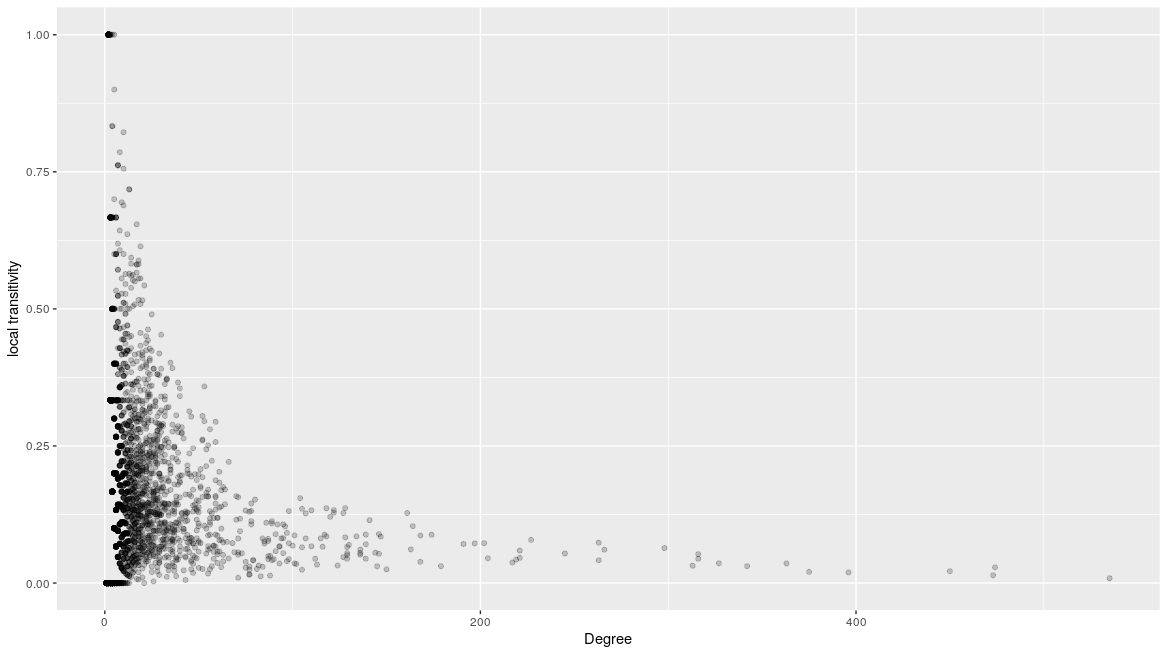
\includegraphics[width=\textwidth]{images/Rplot02_degree_and_transitivity-change_alpha.png}
    \caption{Scatter plot of the relationship between degree and local transitivity for the PSP nodes. Nodes with degree 1 have transitivity set to zero as transitivity in this case is undefined. Plot appears to show a negative correlation between degree and transitivity. The opacity of points has been decreased to reduce overplotting and show the increase in points at low degree}
    \label{fig:Scatter plot of the relationship between degree and local transitivity for the PSP nodes}
\end{figure}
\begin{figure}
    \centering
    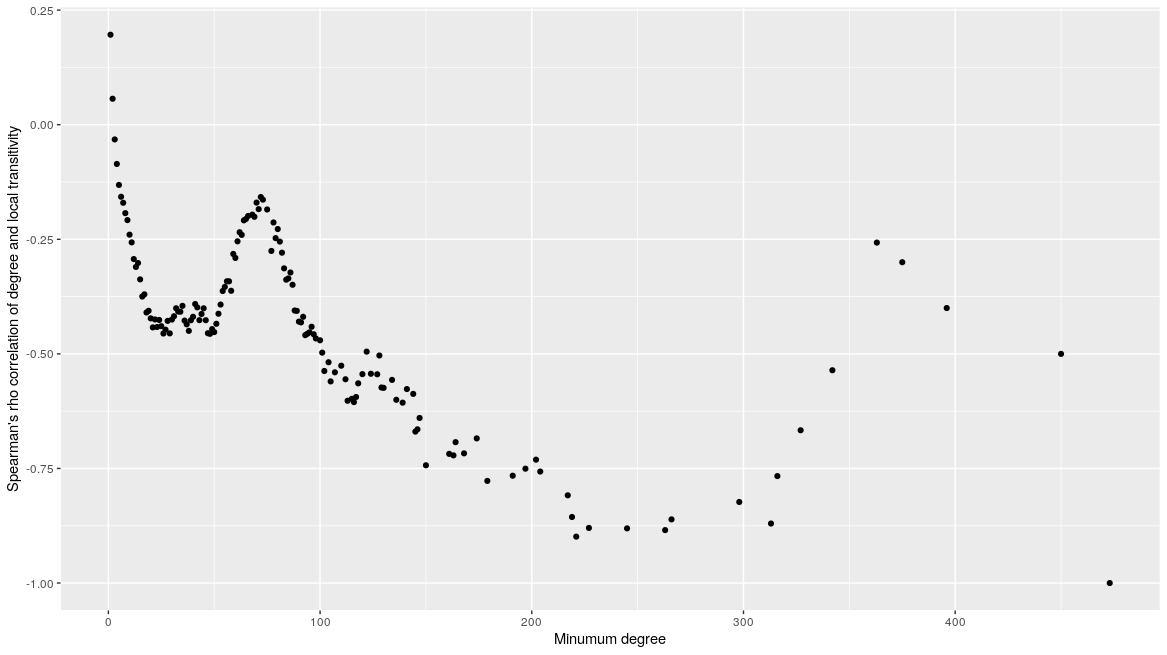
\includegraphics[width=\textwidth]{images/Rplot01_min_degree_transitivity.png}
    \caption{Plot of minumum degree included in the calculation of Spearmans rank correlation between degree and $\rho$. Although the overall coefficient is positive the correlation for nodes above degree 5 are clearly negative and this becomes more apparent at high degree. This relationship is therefore complex and the typical relationship described in the literature may only hold for the large networks in which this relationship has been studies such as the internet. }
    \label{fig:Plot of minumum degree included in the calculation of Spearmans rank correlation between degree and rho}
\end{figure}

The global undirected transitivity of the PSP network is 0.0697. This is similar to the value reported in p305 Newman \cite{newman2018networks} for metabolic networks (0.090) and PPI (0.072)\todo{check both different global formRplotulae in Newman}.\todo{describe method}

The expected value of the global clustering coefficient with a given degree distribution connected randomly \cite{newman2018networks} p332 is:
\begin{equation}
    C=\frac{1}{n}\frac{[<k^2> - <k>]^2}{<k^3>}
\end{equation}

The value of this for the PSP is 0.004541763 \footnote{code \url{source('~/RProjects/centrality/R/transitivity/Expected_global_transitivity.R')}}. The global clustering coefficient is therefore high. Newman states p334 \cite{newman2018networks} that it is not clear why certain non social networks have higher than expected global clustering (for social networks it is ascribed to social choice). For other networks such as the internet with very right skewed degree distribution the clustering coefficient is less than expected. For biological systems such as food webs or the world wide web it is hypothesised that this may due to community formation (newman ref 367)

Also motifs (other than number of triangles) newman 334 again

\subsubsection{Local clustering coefficient Results}
Local clustering coefficient tends to be inversely proportional to degree. It is undefined for nodes of degree one. See~figure \ref{fig:log_transitivity_degree}. It is suggested that this may also be due to community formation \cite{newman2018networks} p335.

Mean local transitivity is 0.171. The distribution is right skewed with median of 0.129 and 3rd quartile of 0.23 and first quartile of 0.043. This does not match the arithmetic mean of vertex local clustering below it may be down to how we deal with NA. Above calculated as NA.rm
\subsubsection{Results GO enrichment local clustering coefficient}

There was little enrichment for local clustering coefficient using GO and 0.05 and 0.95 centile in part because of the large number of 0 values when isolates are treated as 0. However in table~\ref{tab:Number of nodes 935 local transitivity 0.05 centile  local transitivity $<=$ 0 CC background PSP.Alpha=3.33555703802535e-05isolates 0} we can see that low local transitivity i.e. transitivity equal to 0 nodes (isolates) are enriched for plasma membrane components, the plasma membrane components do not show marked transitivity which is perhaps to be expected as they are at the edge of the PSP and it would not be intuitive for these components to all be interconnected. 


\subsection{kcoreness results}
 The minimum shell index is 1, all of the 1 kcore corresponds to the connected component. The range of shell index is 1-24. The median shell index of a vertex is 8 and the mean value 9.15 (although shell indexes take on integer values). The distribution of these values is shown in figure~\ref{fig:Kcore_histogram}\todo{nice ish image of kcore already in core periphery section}
 
 \begin{figure}
     \centering
     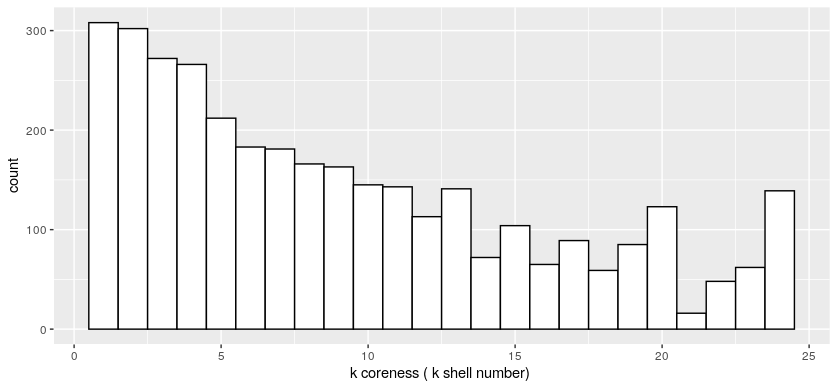
\includegraphics[width=\textwidth]{images/Rplot01_kcore_hist.png}
     \caption{Histogram of shell index of vertices in calculation of kcore. Shell index is the maximum kcore a vertex is a member of and not a member of shell index n+1. }
     \label{fig:Kcore_histogram}
 \end{figure}
 
 
 \subsubsection{K core gene ontology}
 
 Gene ontology enrichment for molecular  a range over the outer core 1-7 is shown in table~\ref{tab:kcore range GO Number of nodes 1724 k core 0 centile  k core1-7 MF background PSP. Alpha=3.33555703802535e-05}. It shows enrichment for trans-membrane transporters and G protein coupled receptors. 
 
 The innermost core $k>=23$ shows enrichment for RNA processing as seen in other centrality measures (table~\ref{tab:Number of nodes 201 k core 0.95 centile  k core $>=$ 23 BP background PSP. Alpha = 4.5583006655119e-06})

Code for GO and centrality measures \url{source('~/RProjects/group_sizes/R/plotting/modified_example...'} 
 
 

\section{Correlation of centrality measures}

For correlation of centrality measures see table~\ref{tab:Correlation between vertex centrality measures for PSP. Spearman's rho}

%%%% REMOVED MISSING EIGENVECTOR CENTRALITY

% % latex table generated in R 3.6.2 by xtable 1.8-4 package
% % Fri Feb 14 12:11:44 2020
% \begin{table}[ht]
% \centering
% \begin{tabular}{rrrrrr}
%   \hline
%  & degree & betweenness & transitivity & closeness & kcoreness \\ 
%   \hline
% degree & 1.000 & 0.902 & 0.196 & 0.851 & 0.986 \\ 
%   betweenness & 0.902 & 1.000 & $-0.002^*$ & 0.782 & 0.854 \\ 
%   transitivity & 0.196 & $-0.002^*$ & 1.000 & 0.292 & 0.265 \\ 
%   closeness & 0.851 & 0.782 & 0.292 & 1.000 & 0.872 \\  
 

%   kcoreness & 0.986 & 0.854 & 0.265 & 0.872 & 1.000 \\ 
%   \hline
% \end{tabular}
% \caption{Correlation between vertex centrality measures for the post synaptic proteome network. Spearman's rho. All $p < 2.2 x 10^{-16}$ other than * $p=0.90$} 
% \label{tab:Correlation between vertex centrality measures for PSP. Spearman's rho}
% \end{table}


% latex table generated in R 3.6.3 by xtable 1.8-4 package
% Sat Jun 13 15:27:48 2020
\begin{table}[ht]
\centering
\begin{tabular}{rrrrrrr}
  \hline
 & Degree & Eigenvector & Closeness & Betweenness & Transitivity & Kcore \\ 
  \hline
Degree & 1.00 & 0.88 & 0.85 & 0.90 & 0.38 & 0.99 \\ 
  Eigenvector & 0.88 & 1.00 & 0.97 & 0.76 & 0.46 & 0.91 \\ 
  Closeness & 0.85 & 0.97 & 1.00 & 0.78 & 0.43 & 0.87 \\ 
  Betweenness & 0.90 & 0.76 & 0.78 & 1.00 & 0.21 & 0.85 \\ 
  Transitivity & 0.38 & 0.46 & 0.43 & 0.21 & 1.00 & 0.43 \\ 
  Kcore & 0.99 & 0.91 & 0.87 & 0.85 & 0.43 & 1.00 \\ 
   \hline
\end{tabular}
\caption{Correlation matrix method spearman for centrality scoresAll $p < 2.2 x 10^{-16}$. Code at \url{source('~/RProjects/centrality/R/correlation_centrality_measures/correlation_centrality_measures.R')}}
\label{tab:Correlation between vertex centrality measures for PSP. Spearman's rho}
\end{table}

\begin{figure}
    \centering
    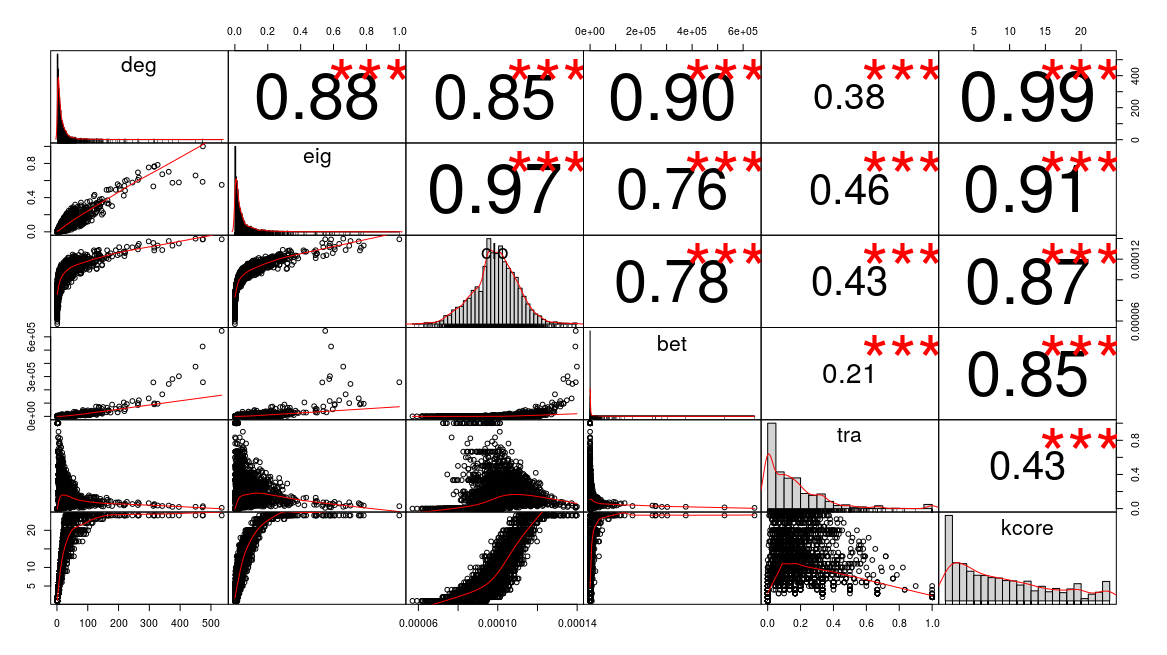
\includegraphics[width=\textwidth]{Rplot_corr_spearman_using_package_performance_analytics.png}
    \caption{Correlation plot of centrality measures using package Performance Analytics. Deg = degree, eig= eigenvector centrality, clo = closeness centrality, bet = betweenness centrality, tra = local transitivity, kcore = kcoreness}
    \label{fig:Correlation plot centrality performance analytics}
\end{figure}



All of the centrality measures are correlated with each other other except transitivity and betweenness centrality  (table~\ref{tab:Correlation between vertex centrality measures for PSP. Spearman's rho}). Transitivity is most weakly correlated with other measures. Code \footnote{\url{source('~/RProjects/paper_xls_output/R/make_df_correlation_between_centrality_measures.R')}}
\todo{move comparison here}



See \cite{oldham2019consistency} for correlation across networks. See table~\ref{tab:Correlation of centrality valente et al}

\subsection{Normality of correlation measures}
% latex table generated in R 3.6.3 by xtable 1.8-4 package
% Sat Jun 13 15:54:02 2020
All of the centrality measures appear to vary from a normal distribution using the Shaprio-Wilk test in R and in accordance with their plots. Spearmans test of correlation will therefore be used for correlation with centrality measures (table~\ref{tab:Shapiro-Wilk test for normality of centrality measures}

\begin{table}[ht]
\centering
\begin{tabular}{lrr}
  \hline
Centrality measure & W & p value \\ 
  \hline
Degree & 0.425 & $2.517 \times 10^{-74}$ \\ 
  Eigenvector\_centrality & 0.561 & $6.553 \times 10^{-69}$ \\ 
  Closeness & 0.995 & $4.686 \times 10^{-9}$ \\ 
  Betweenness & 0.123 & $2.764 \times 10^{-83}$ \\ 
  Local transitivity & 0.775 & $2.653 \times 10^{-56}$ \\ 
  kcore & 0.911 & $4.321 \times 10^{-41}$ \\ 
   \hline
\end{tabular}
\caption{Shapiro-Wilk test for normality of centrality measures. Code at \url{source('~/RProjects/centrality/R/correlation_centrality_measures/shapiro-wilk.R')}} 
\label{Table:Test for normality (Shapiro-Wilk) for centrality measures of PSP}
\end{table}

\subsection{Results of correlation analysis FROM PAPER}
\textcolor{red}{Moved from earlier}
The vertex measures are correlated with one another apart from transitivity and range from 0.89 (eigenvector centrality and degree) to 0.33 (betweenness centrality and closeness centrality) (\textcolor{red}{see supplementary table 6} \todo{table}).
There is a weak negative ($\rho \approx 0.2$) correlation between 
the degree of selection pressure a gene is under and all measures of vertex importance except for transitivity (\textcolor{red}{see table 7 supplemental material} \todo{table}).
Although nodes of high importance or local clustering do have distinct properties, for example nodes with degree $> 50$ are enriched in association for the biological process (GO:1903350)‚ ”intracellular response to dopamine‚” (FDR P= 2.10 $\times 10^{-4}$ fold change 22.37), we find no correlation with these measures and genetic association with educational attainment or intelligence. 
\textcolor{green}{DRAFT -something like This is not because nodes of high degree or other centrality measure do not share common attributes, for example nodes with degree $>50$ are disproportionately found in BP intracellular dopamine but we find no association between these measures and educational attainment or intelligence}





\subsection{RESULTS Assortativity and methods degree assortativity}
\textcolor{red}{Move to discussionj}We can compare the average degree with those found in other publications. We can also look at the assortativity between nodes for degree. The PSP networks shows evidence of some negative degree assortativity (-0.18) using the commands \texttt{assortativity(g,deg,directed=FALSE)} in igraph for R \todo{Assortativity for essential and id}.

The degree association is negative in most real world networks other than social networks \cite{newman2002assortative}. \todo{include the peel multi-scale mixing patterns} see table \ref{Table:DegreeAssortativityNewman}\todo{? add positive $r$ to table}. Both the Barabsi Albert model and random model have 0 correlation. The Callaway model of network generation ('grown graph' - newman) has a positive degree correlation consistent with older nodes being connected to each other and hence in turn being more likely to be connected to others. This is at odds with our later finding (see orthologues) that nodes with clearly identified yeast orthologues tend to be of higher degree (this would fit both the Barabasi Albert model and Callaway) \todo{this is the bit where the pseudohub bit would fit}. 

The assortativity suggests that the Barabasi Albert model is 'incomplete' as a model of the internet \cite{newman2002assortative} and in this network we also find evidence that our synaptic protein protein interaction has similar degree assortativity to that calculated by Newman which is of the yeast interactome (cite Jeong) . The reasons for this are not clear, there are other things in our study that support the Barabasi model and it may be that multiple processes are taking place. \todo{? move this to discussion}

The value of $r$ of -0.18 \todo{three sf} is similar to those cited by Newman \cite{newman2002assortative} in table \ref{Table:DegreeAssortativityNewman}. 

Although we expect the assortativity to be 0 in a random graph of the configuration model (the edges are placed at random so we would not expect there to be any association with edges and the degree of vertices), there will nevertheless be a deviation from 0 due to chance and it is helpful to quantify the assortativity by calculating this. 

The assortativity using a configuration model \todo{explain configuration model} is approximately normal centred on 0.
\textcolor{red}{table}
For 10,000 samples   

Min.    1st Qu.     Median       Mean    3rd Qu.       Max. 
-2.142e-02 -3.811e-03 -1.743e-05  5.524e-05  3.861e-03  2.235e-02 

Shapiro-Wilk normality test

data:  results[1:500]
W = 0.99538, p-value = 0.1446


\begin{table}[]
    \centering
    \begin{tabular}{c|c|c}
       network  &N& $r$  \\
       \hline
       internet & 10697&-0.189\\
       world wide web &269504 & -0.065\\
       post synaptic proteome & 3457 & -0.18\\
       protein interactions & 2115 & -0.156\\
       neural network & 307 & -0.163\\
       food web & 92 & -0.276 \\
       
       
         
    \end{tabular}
    \caption{Degree assortativity coefficients of networks adapted from Newman 2002 \cite{newman2002assortative} including post synaptic proteome}
    \label{Table:DegreeAssortativityNewman}
\end{table}

%\subsubsection{Degree correlation}
 
\todo{Include \url{R_plot_degree_correlation.png} commented out}


Newman \cite{newman2018networks} p336 cites Maslov \cite{maslov2004detection} as giving as a reason for the disassortative nature of many empirical networks the prohibition on multi-edges. The expected number of multiedges between nodes would be greater than one (need to look at the paper again).

This is possibly the bit where Keith's bit would be good to put in.  
 %\begin{figure}]h]
 % \includegraphics[width=\linewidth]{Rplot_degree_correlation.png}
 % \caption{Plot of degree with k nearest neighbour mean of degree}
 % \label{fig:knn_degree}
%\end{figure}
%
%
%

\subsection{Assortativity with gene score}
 
A second way in which we could see if genes within the PSP that are enriched for genetic differences in education and intelligence globally within the PSP would be to calculate the correlation between there being and edge between two vertices and the significance score of the two vertices. A positive result would suggest that more significant (avoiding a cutoff effect) genes have protein products that are more likely to interact in the PSP graph. We can do this by calculating the assortativity as described by Newman. As a measure of significance we use the z score for each gene in the PSP for each study as provided by MAGMA. As some genes in the PSP do not have a significant number of SNPs within them they do not have a Z score as assigned by magma and these are therefore set to 0. \footnote{code \url{source('~/RProjects/centrality/R/get_gene_scores/assortativity_with_z_scores.R')} }

\subsubsection{Assortativity with z score results}
 
 \begin{table}[]
     \centering
     \begin{tabular}{ccc}
     \toprule
         Study & Missing values  & Assortativity\\
         \midrule
         Intelligence\textsubscript{Replication} & 148 & 0.003\\
         Education\textsubscript{Replication} & 172 & -0.006\\
         Education\textsubscript{Discovery} & 156 & 0.001\\
         Intelligence\textsubscript{Discovery} & 156 & -0.004\\
         \bottomrule
     \end{tabular}
     \caption{Assortativity of PSP graph vertices by study Z score. PSP graph members without corresponding Z score marked as missing values had z set to 0.}
     \label{tab:Assortativity of PSP graph and z scores}
 \end{table}


The results are shown in table\ref{tab:Assortativity of PSP graph and z scores}. Assortativity scores tend to me modest (as score of approximately 0.15 is often found for degree assortativity). These results are close to zero. 

This suggests that nodes with high or low z scores in the population cohorts are no more likely to have links to one another \textit{globally} across the network. It does not state that there cannot be areas within the graph where there are areas of high assortativity or areas where one high score connects to linker node connects to another high score in a group.

\todo{do this with pli too and for a phenotype eg GO glutamate}
\section{Association between significant vertices}
Do there tend to be edges between significant vertices? Do the vertices representing genes of genome wide significance form an induced subgraph that is connected?
The induced subgraph \todo{define} of significant genes for Intelligence\textsubscript{Replication} is 16 vertices no edges. Simulation mean 0.60 sd 0.94 N iterations = 1000. For Education\textsubscript{Replication} it is 25 vertices no edges (simulation mean 1.51 sd 1.69). For Intelligence \textsubscript{Discovery} it is 58 vertices with 4 edges. Simulation mean 8.78 sd 5.13. For Education \textsubscript{Discovery} it is 51 vertices with 2 edges. Simulation mean 6.3 SD 4.1.

Simulation of joint results out of 1000, 100 trials
Min. 1st Qu.  Median    Mean 3rd Qu.    Max. 
   1.00    4.00    6.00    5.98    8.00   14.00 
   
   max = 14/1000 = 0.014
   mean = 0.006 of getting this number of edges or fewer in 4 samples of random subgraphs eg(number of times subgraph is 0 and next is 0 or less and next is 4 or less and next is 51 or less given actual frequency 0,0,4,2 and number of samples 16,25,58,51.
   
 


 
 \todo{Assortativity of essential nodes in PSP}
 \todo{difference plI and DEG}
 
 \subsection{Results from database of essential genes}

2238 genes in the PSP are essential (64.7\%)

This compares with 37.\% of the genome as a whole (assuming 20000 genes \todo{get non essential number from database}. 36.5\% (6043/20000) non PSP genes are essential. 

\subsubsection{Degree and essential genes}

The summary statistics for the degree of essential PSP genes and non essential PSP genes are shown in table~\ref{tab:degree distribution essential and non essential genes PSP}. The mean degree is higher in essential (21.29) vs non essential genes (10.94) $p<2.2 \time 10^{-16}   W=1777916$ Wilcoxon rank sum test with continuity correction in R.

The boxplot of log degree for essential and non essential genes in the PSP is shown in figure~\ref{fig:boxplot_log degree essential genes}
\footnote{code \url{source('~/RProjects/paper_xls_latex/R/essentail_genes/lbxplot_and_latex_essential_genes.R')}}.

The assortativity of essential nodes in the PSP is 0.0438 (ie very mild assortative although they tend to have high degree and PSP degree is disassortative).


\begin{table}[ht]
\centering
\begin{tabular}{rlrrrrrrr}
  \hline
 & name & n & Min. & 1st Qu. & Median & Mean & 3rd Qu. & Max. \\ 
  \hline
1 & Essential & 2238 & 1.00 & 5.00 & 11.00 & 21.29 & 23.00 & 474.00 \\ 
  2 & Non essential & 1219 & 1.00 & 2.50 & 5.00 & 10.94 & 12.00 & 535.00 \\ 
  3 & All & 3457 & 1.00 & 4.00 & 8.00 & 17.64 & 19.00 & 535.00 \\ 
   \hline
\end{tabular}
\caption{Degree distribution of essential and non essential genes in PSP}
\label{tab:degree distribution essential and non essential genes PSP}
\end{table}

\begin{figure}
    \centering
    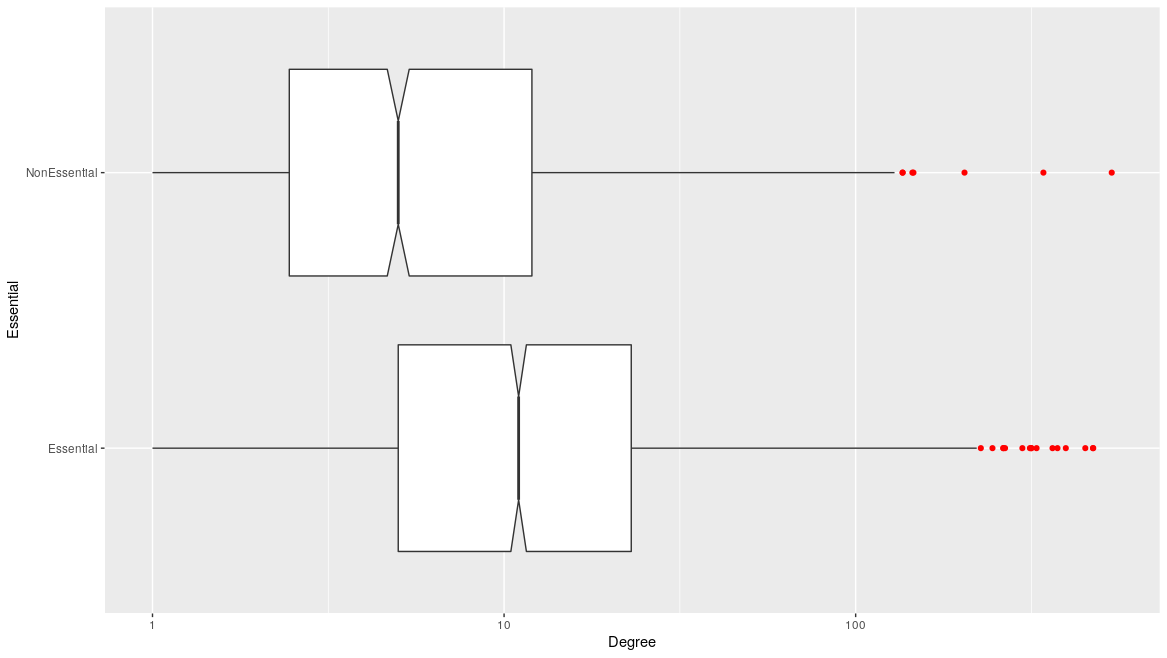
\includegraphics[width=\textwidth]{images/Rplot_essential_non_essential_gene_degree.png}
    \caption{Degree distribution for essential and non essential PSP genes using DEG 15.2. 2238 Essential genes, 1219 Non essential}
    \label{fig:boxplot_log degree essential genes}
\end{figure}



\subsubsection{Essential gene conclusion}
PSP genes are more likely to be essential. Essential genes are of higher degree than non essential genes. There is a very weak assortativity for essential genes. 

\todo{DONE Degree etc for essential genes}
\todo{Essential genes enrichment vs non essential PSP add to community detection section}
\todo{Essential gene count for significant genes vs psp genes}

 \subsubsection{Degree distribution of PSP genes - murine model}
 
 We can use the mouse phenotype ontology to identify essential murine genes. 
 We want to know if high degree PSP nodes are more commonly associated with essentiality in murine models. 
 
 The 90\% centile for PSP gene degree is $k=37$. 349 genes in the PSP network model have degree $k>=37$.
 
 Murine phenotype MP:008763 is embryonic lethality. 117 of the genes with degree $k>=37$ are essential (33.5\% of 349 genes). 458 genes are essential in the remaining PSP nodes ($k < 37$, 458 of 3108 14.7\%). p $3.13 \times 10^{-11}$ Fisher's exact test for count data R. Odds ratio 2.27 95\% CI 1.79-2.88. \footnote{code:\url{/home/grant/RProjects/phenome_and_network/R/get_degree_90_quantile_PSP.R}} \todo{Calculate difference in degree for essential versus not essential} Comment \todo{one reason for testing the top 10\% is that the degree distribution is of a few hubs (cite Jeong) with different properties from the rest given the scale free structure of the network}
 
 \begin{table}[h]
     \centering
     \begin{tabular}{llllll}
          Title & $k$& n essential & n & percentage essential & p   \\
          \hline
          Top 10\% & $>=37$ & 117 & 349 & 33.5 & $3.13 \times 10^{-11}$\\
          Rest & $<37$ & 458 & 3108 & 14.7 & \\
     \end{tabular}
     \caption{Association of high degree nodes with being essential in murine models. Genes with degree in top 10\% of PSP compared with the rest. P Fisher's Exact Test for Count data.}
     \label{Table:Degree and murine essentialness PSP}
 \end{table}
 

\todo{GO enrichment with background PSP for high degree are in \url{/home/grant/Dropbox/stront_share/data/GO\_high\_degree_psp_background}}




\subsection{Degree and orthologs}

If the network is generated by the preferential attachment model of Barabasi we would expect the nodes of high degree to have more ancient orthologues than those of lower degree.  Duplication divergence \todo{ref} may be an important mechanism as we know there was a genome duplication event nevertheless we could hypothesise that the nodes with yeast orthologues will have higher median degree than the human and murine PSP. \todo{add cross ref to orthologues}

\section{Probability of loss of function intolerance (pLI)}

\todo{Remove takehome} \subsubsection{Takehome: Remove}

The probability of loss of function intolerance is associated with measures of vertex centrality in the post synaptic proteome graph. The correlation is greatest for degree ($\rho=0.230$) and lowest for transitivity ($\rho=0.086$). Betweenness and eigenvector centrality have similar correlation to loss of function intolerance as degree (see table \ref{Table:Correlation of pLI with centrality vertex statistic})



\subsection{Distribution of pLI and intelligence}
\todo{Distribution of pLI and intelligence}


% latex table generated in R 3.6.2 by xtable 1.8-4 package
% Sat Jan 11 15:09:57 2020
\begin{table}[ht]
\centering
\begin{adjustbox}{max width=\textwidth}
\begin{tabular}{rllrrrl}
  \hline
 & Study & Graph statistic & S & p & rho & Test \\ 
  \hline
1 & Intelligence Discovery & pLI & $5.400 \times 10^{9}$ & $1.10 \times 10^{-6}$ & -0.087 & Spearman's rank correlation rho \\ 
  2 & Intelligence Replication & pLI & $5.200 \times 10^{9}$ & $1.07 \times 10^{-2}$ & -0.046 & Spearman's rank correlation rho \\ 
  3 & Education Discovery & pLI & $5.600 \times 10^{9}$ & $1.38 \times 10^{-11}$ & -0.120 & Spearman's rank correlation rho \\ 
  4 & Education Replication & pLI & $5.200 \times 10^{9}$ & $1.54 \times 10^{-4}$ & -0.068 & Spearman's rank correlation rho \\ 
   \hline
\end{tabular}
\end{adjustbox}
\caption{Correlation of GWAS gene level statistics Spearman's rho gene pLI} 
\label{Table:Correlation of GWAS gene level statistics Spearmans rho gene pLI}
\end{table}

% latex table generated in R 3.6.2 by xtable 1.8-4 package
% Fri Mar  6 15:52:12 2020
\begin{table}[ht]
\centering
\begin{adjustbox}{max width=\textwidth}
\begin{tabular}{llrrr}
  \hline
study & comparison & rho & S & p \\ 
  \hline
Intelligence Replication & all Zstat and pLI & 0.043 & 797235155436.9 & $2.358 \times 10^{-8}$ \\ 
  Intelligence Replication & synaptic Zstat and pLI & 0.042 & 5465708502.3 & $1.661 \times 10^{-2}$ \\ 
  Intelligence Replication & non synaptic Zstat and pLI & 0.033 & 428265764841.3 & $1.249 \times 10^{-4}$ \\ 
  Education Replication & all Zstat and pLI & 0.065 & 749149170637.4 & $4.370 \times 10^{-17}$ \\ 
  Education Replication & synaptic Zstat and pLI & 0.070 & 5198989756.7 & $6.926 \times 10^{-5}$ \\ 
  Education Replication & non synaptic Zstat and pLI & 0.059 & 398992399833.6 & $6.604 \times 10^{-12}$ \\ 
  Intelligence Discovery & all Zstat and pLI & 0.066 & 778515153123.3 & $8.384 \times 10^{-18}$ \\ 
  Intelligence Discovery & synaptic Zstat and pLI & 0.078 & 5218943442.6 & $7.746 \times 10^{-6}$ \\ 
  Intelligence Discovery & non synaptic Zstat and pLI & 0.048 & 422374139606.0 & $1.396 \times 10^{-8}$ \\ 
  Education Discovery & all Zstat and pLI & 0.093 & 755468138230.8 & $2.195 \times 10^{-34}$ \\ 
  Education Discovery & synaptic Zstat and pLI & 0.117 & 5003003452.8 & $2.793 \times 10^{-11}$ \\ 
  Education Discovery & non synaptic Zstat and pLI & 0.071 & 412373757794.5 & $7.820 \times 10^{-17}$ \\ 
   \hline
\end{tabular}
\end{adjustbox}
\caption{Extra table to be removed shows spearman for all synaptic and non synaptic and all but rho is with pLI and zstat not -log10 and -log10 of p  so rho is positive ie}
\label{tab:Extra table to be removed shows spearman for all synaptic and non synaptic and all but rho is with pLI and zstat not -log10 and -log10 of p  so rho is positive ie}
\end{table}

There was a weak association between probability of loss of function intolerance and gene score in this case z score. In table \ref{Table:Correlation of GWAS gene level statistics Spearmans rho gene pLI} the correlation is shown with the negative log10 transform of the p value and so $\rho$ is negative. Fuller results are shown in table ~\ref{tab:Extra table to be removed shows spearman for all synaptic and non synaptic and all but rho is with pLI and zstat not -log10 and -log10 of p  so rho is positive ie}  \footnote{\url{source('~/RProjects/paper_xls_output/R/make_df_correlation_pLI_genescore.R')}} the relationship is stronger for synaptic genes than for non synaptic genes although the effect is small and synaptic genes as shown below have a higher probability of loss of function intolerance.
\todo{visualisation or graph}
There was a positive correlation between loss of function intolerance and the gene Z stat. To be explicit the Z stat is high and positive when the gene has a more significant association with the phenotype and hence a lower p value. There is a weak association between high loss of function intolerance and significant (low p value genes)

\todo{there is something wrong here as Jan we find correlation} 
 In testing correlation spearman’s rank correlation was used as the distribution of the probability of loss of function intolerance statistic is very non linear. It has a bi-modal distribution (see figure~\ref{fig:density estimate pLi} with a concentration of probability mass around 0 and 1 .


The distribution of probabilitity of loss of function intolerance in non PSP genes is still bimodal but the probability mass around 1 is much less peaked and there is greater mass at the bottom of the distribution (see figure~\ref{fig:density estimate pLi two panel}. The boxplot in figure ~\ref{fig:Boxplot of pli} shows the median and means of the distributions\footnote{ Source for graphs \url{source('~/RProjects/paper_xls_output/R/plot_pli_PSP_v_restgenome.R')}}. 


\begin{figure}
    \centering
    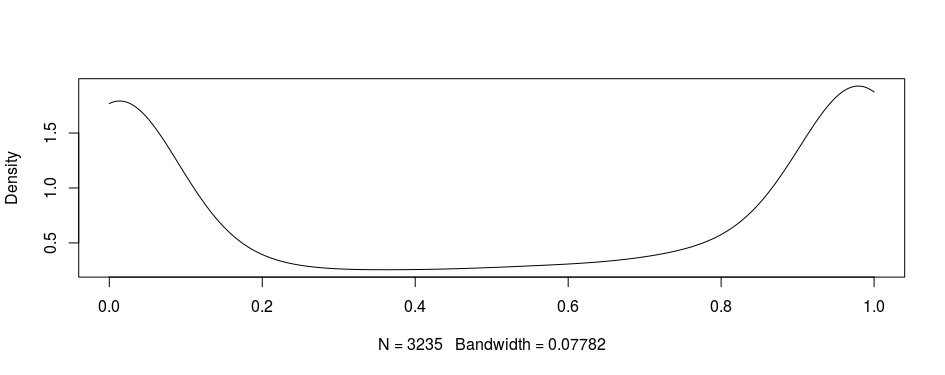
\includegraphics[width=0.9\textwidth]{images/Rplot_kernel_density.png}
    \caption{The distribution of probability of loss of function intolerance. Kernel density estimate using Guassian kernel. Bimodal distribution with peak close to 0 and 1 for the post synaptic proteome. }
    \label{fig:density estimate pLi}
\end{figure}

\begin{figure}
    \centering
    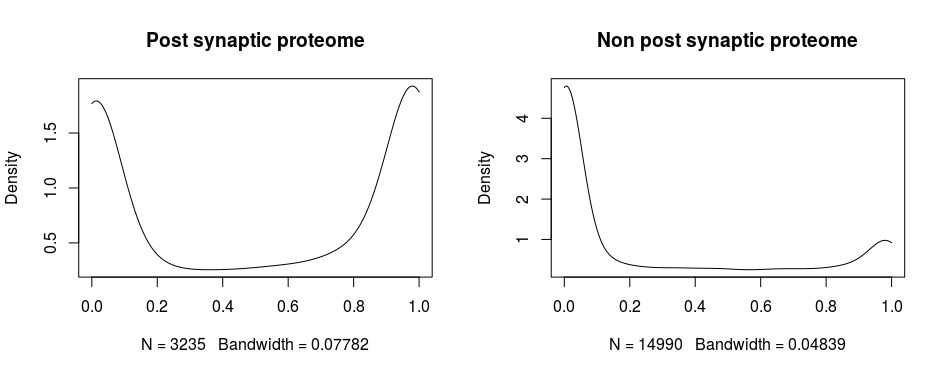
\includegraphics[width=0.9\textwidth]{images/Rplot01_density_PSP_two_panel_nonPSP.png}
    \caption{The distribution of probability of loss of function intolerance for the post synaptic proteome (left) and the rest of the genome (post synaptic proteome removed) on the right. Kernel density estimate using Guassian kernel. Bimodal distribution with peak close to 0 and 1 for the post synaptic proteome. The peak around 1 is much smaller in the non post synaptic proteome. }
    \label{fig:density estimate pLi two panel}
\end{figure}



This code \url{source('~/RProjects/paper_xls_output/R/make_pLI_correlation.R')}
makes the table for the correlation between pLI and vertex statistics. It is the only one found in the previous hard copy so suggest \todo{Redo from scratch correlation between pLI and study p vals to confirm although findings makes sense and cannot inf any previous source code}.

The current results suggest that the relationship between the variables is as shown in the factor graph in figure \ref{Figure:Factor graph for relationship between pLI, vertex statistic and study p values}

\begin{figure}
    \centering
    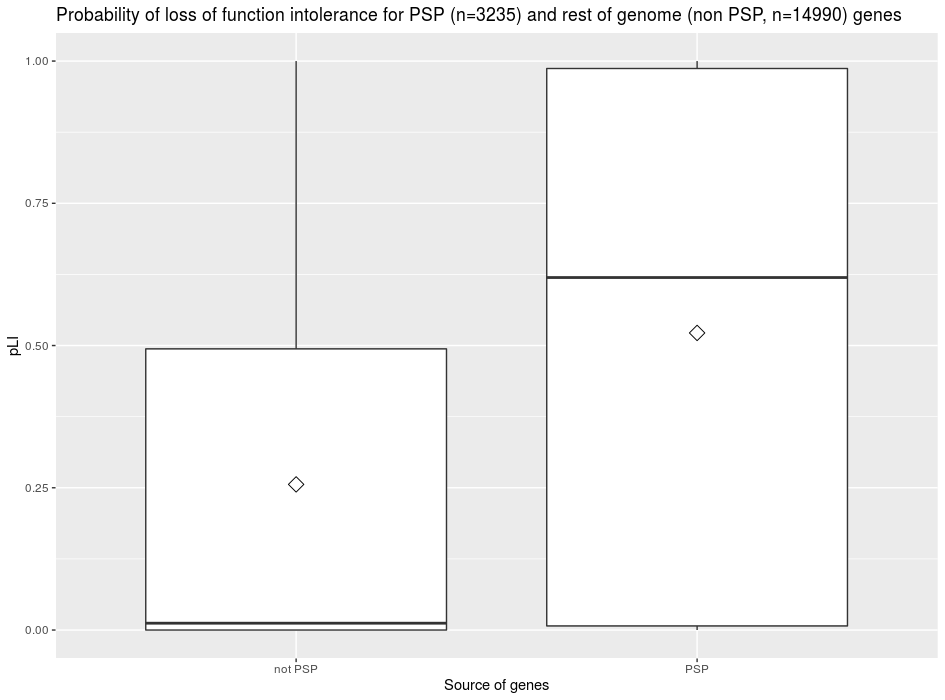
\includegraphics[width=0.9\textwidth]{images/Rplot03_boxplot_pLI_PSP_non_PSP.png}
    \caption{Box plot of probability of loss of function intolerance (pLI) between PSP genes (n=) and non PSP genes (rest of genome n=14990 ). Diamond marker indicates mean PSP value. }
    \label{fig:Boxplot of pli}
\end{figure}

\begin{figure}
    \centering
    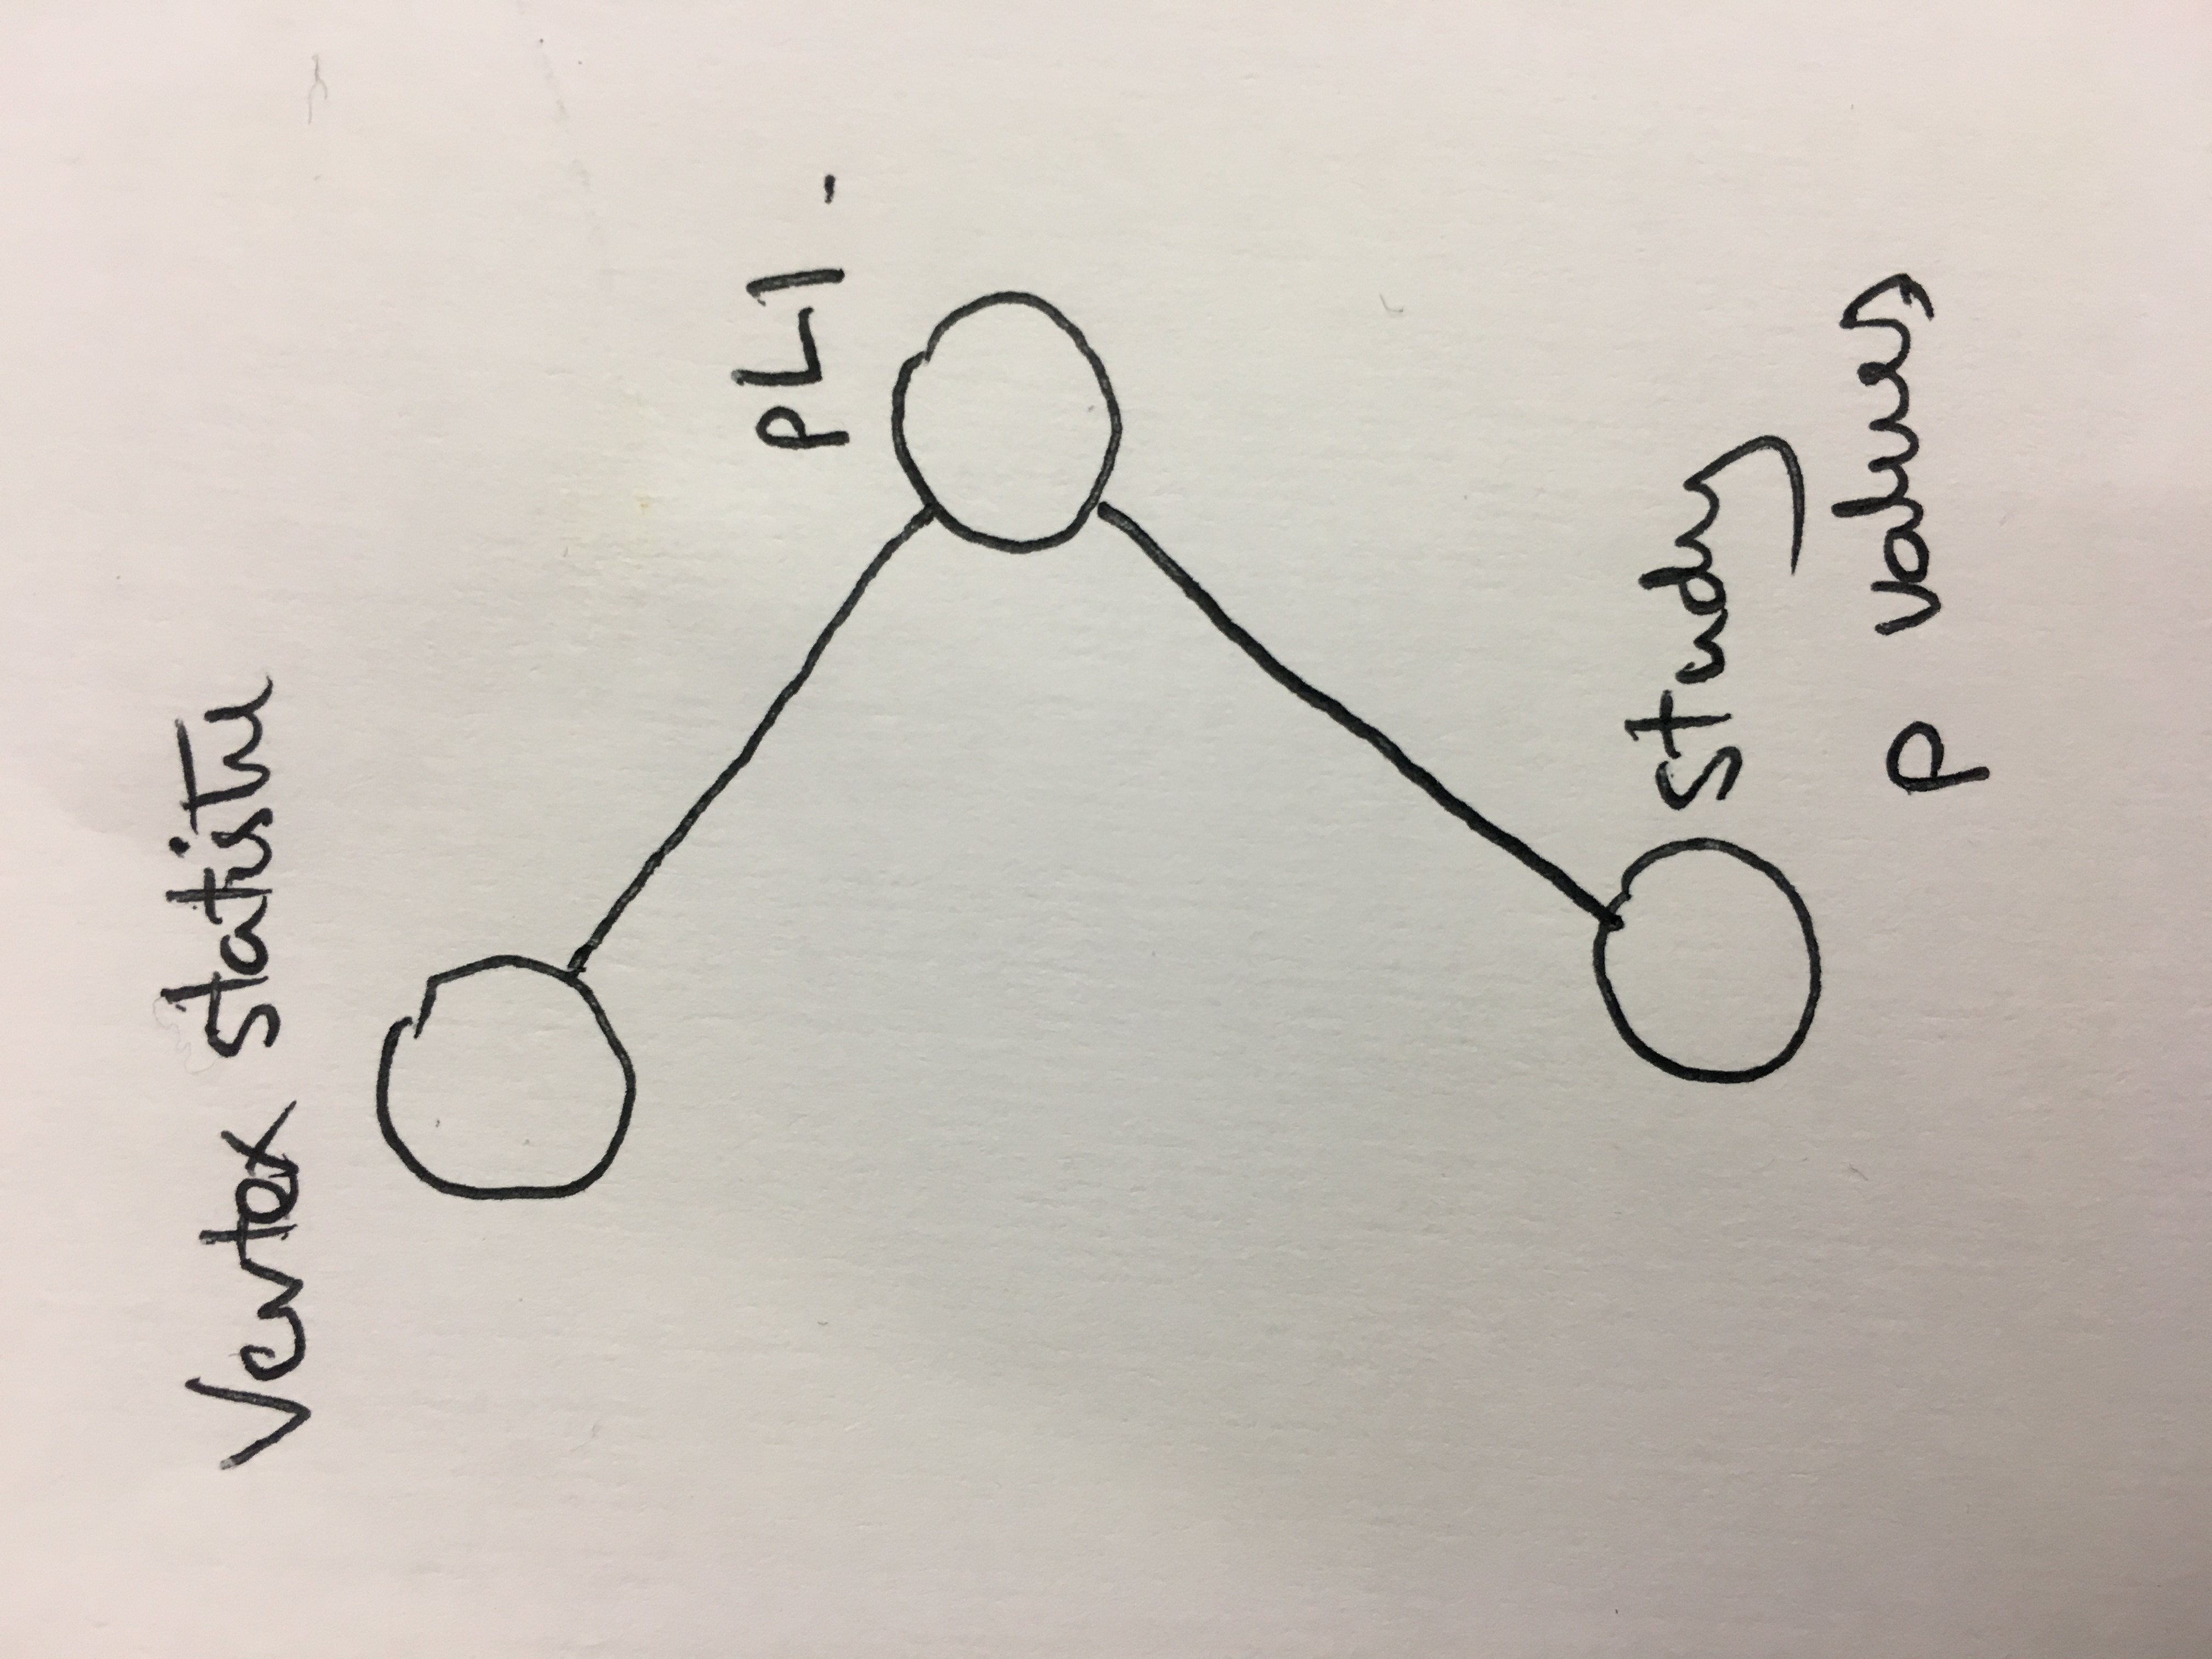
\includegraphics[width=\textwidth]{IMG_6979.JPG}
    \caption{Factor graph for relationship between pLI, vertex statistic and study p values}
    \label{Figure:Factor graph for relationship between pLI, vertex statistic and study p values}
\end{figure}
\todo{Make into table}
% latex table generated in R 3.6.2 by xtable 1.8-4 package
% Sat Jan 11 15:52:39 2020
\begin{table}[ht]
\centering
\begin{tabular}{rllrrrl}
  \hline
 & Study & Graph statistic & S & p & cor & Test \\ 
  \hline
1 & pLI & Degree & $4.300 \times 10^{9}$ & $2.00 \times 10^{-40}$ & 0.230 & Spearman's rank correlation rho \\ 
  2 & pLI & Betweenness & $4.500 \times 10^{9}$ & $1.40 \times 10^{-32}$ & 0.210 & Spearman's rank correlation rho \\ 
  3 & pLI & Eigenvector & $4.400 \times 10^{9}$ & $6.60 \times 10^{-37}$ & 0.220 & Spearman's rank correlation rho \\ 
  4 & pLI & Transitivity & $4.000 \times 10^{9}$ & $2.80 \times 10^{-6}$ & 0.086 & Spearman's rank correlation rho \\ 
   \hline
\end{tabular}
\caption{Correlation of pLI with centrality vertex statistic. Code \url{source('~/RProjects/paper_xls_output/R/get_exac_correlation.R')}} 
\label{Table:Correlation of pLI with centrality vertex statistic}
\end{table}
\subsubsection{pLI and vertex statistics}
 The   correlation between pLI and vertex statistics is shown in table table \ref{Table:Correlation of pLI with centrality vertex statistic} \footnote{ code at \url{source('~/RProjects/paper_xls_output/R/make_pLI_correlation.R')}}. This suggests that a correlation between centrality measure and loss of function intolerance where more important genes in terms of centrality measure are more likely to be intolerant of genetic change. The correlation is greatest for degree ($\rho = 0.23$) but is similar for betweenness centality and eigenvector centrality. The correlation is much weaker for transitivity. 
 
 
\subsubsection{Linear model of pLI and vertex statistics}    
A linear regression model for centrality measures and pLI was constructed \footnote{Code \url{source('~/RProjects/paper_xls_output/R/make_pLI_correlation.R')}}. Although the correlation may be similarly linear the eigenvector centrality may have more effect on the gradient of the line of the relationship. 

The eigenvector centrality seems to predict pLI best. Taking the 3rd quartile of the eigenvector centrality then the following are the summary statistics for the pLI

The genes with higher eigenvector centrality tend to have higher probability of loss of function intolerance see table~\ref{tab:pli and eigenvector centrality quartiles}

\begin{table}[]
    \centering
    \begin{tabular}{llllllll}
    \toprule
      Sample &  Min. &1st Qu.&  Median &   Mean& 3rd Qu.&    Max. &   NA's     \\
      \midrule
     Eigenvector 3rd quartile  &0& 0.349& 0.9315& 0.689& 0.998& 1&     48  \\ 
     PSP &0&0.007&0.620&0.522&0.987&  1 & 222\\
     Eigenvector less than 3rd quartile &0&0.002&0.386&0.466&0.974&1&    174\\
     \bottomrule
    \end{tabular}
    \caption{Probability of loss of function intolerance for different values of eigenvector centrality and for PSP as whole}
    \label{tab:pli and eigenvector centrality quartiles}
\end{table}
%   Min. 1st Qu.  Median    Mean 3rd Qu.    Max.    NA's 
% 0.0000  0.3485  0.9315  0.6892  0.9983  1.0000      48 

%For the PSP as a whole this is	
%  Min. 1st Qu.  Median    Mean 3rd Qu.    Max.    NA's 
%0.00000 0.00719 0.61952 0.52215 0.98691 1.00000     222 

%and for the eigenvector centrality below the third quartile it is

%  Min. 1st Qu.  Median    Mean 3rd Qu.    Max.    NA's 
%0.00000 0.00165 0.38598 0.46570 0.97380 1.00000     174

Wilcoxon test for difference in means for all synaptic pLI and those with eigenvector centrality above the third quartile
        Wilcoxon rank sum test with continuity correction

data:  df\$pLI and joined\_df\_synaptic\$pLI
W = 1611226, p-value $< 2.2e-16$
alternative hypothesis: true location shift is not equal to 0


\subsection{pLI for orthologs} \url{source('~/RProjects/orthologs2/R/make_PLI_orthologs.R')}

\todo{Unite this bit with the other ortholog bit}
\todo{Check if this is synaptic and add number}
\begin{table}[ht]
    \centering
    \begin{tabular}{lcccccc}
    &                 Min.& 1st Qu. &Median& Mean& 3rd Qu.& Max.\\
yeast\_sum   &     1.3e-23& 2.5e-02&  0.710& 0.56&    0.98 &   1\\
cel\_sum     &     2.9e-40& 1.3e-02&  0.630& 0.52&    0.97 &  1\\
fly\_sum      &    9.6e-51 &1.9e-02&  0.720& 0.56&    0.99 &  1\\
zf\_sum        &   9.6e-51& 1.1e-02&  0.670& 0.53&    0.99  &  1\\
mouse\_pLI      &  5.4e-91 &6.0e-03&  0.620& 0.52&    0.99   &1\\
pli\_synaptic\_sum & 5.4e-91 &7.2e-03&  0.620& 0.52&    0.99  &  1\\
human\_genome\_plI &5.4e-91 &3.2e-05&  0.028& 0.30&    0.68  &  1\\
  
    \end{tabular}
    \caption{Distribution of pLI (probability of loss of function intolerance orthologs}
    \label{tab:pLI orthologs}
\end{table}



    
\begin{figure}
    \centering
    \begin{subfigure}[t]{0.45\textwidth}
        \centering
        \includegraphics[width=\linewidth]{images/Rplot_transitivity.png} 
        \caption{Histogram of transitivity} \label{fig:transitivity}
    \end{subfigure}
    \hfill
    \begin{subfigure}[t]{0.45\textwidth}
        \centering
        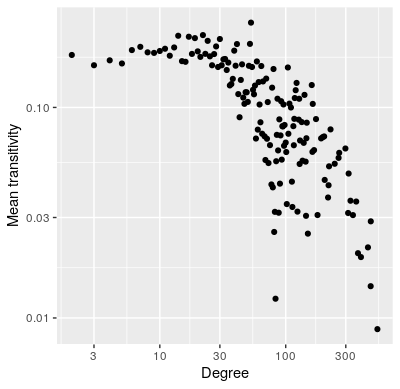
\includegraphics[width=\linewidth]{images/Rplot01_logdegree_log_transitivity.png} 
        \caption{Plot of degree with mean local transitivity. Log10-log10 scale. Omitting degree $k=1$ as transitivity $C$ will be undefined.} \label{fig:log_transitivity_degree}
    \end{subfigure}
    \caption{Plots of transitivity \textcolor{red}{may want to do this in subfigure packages rather than subcaption to line up edges}}
\end{figure}



%\begin{figure}]h]
%  \includegraphics[width=\linewidth]{Rplot_transitivity}
%  \caption{Transitivity}
%  \label{fig:transitivity}
%\end{figure}
 
%\begin{figure}]h]
%  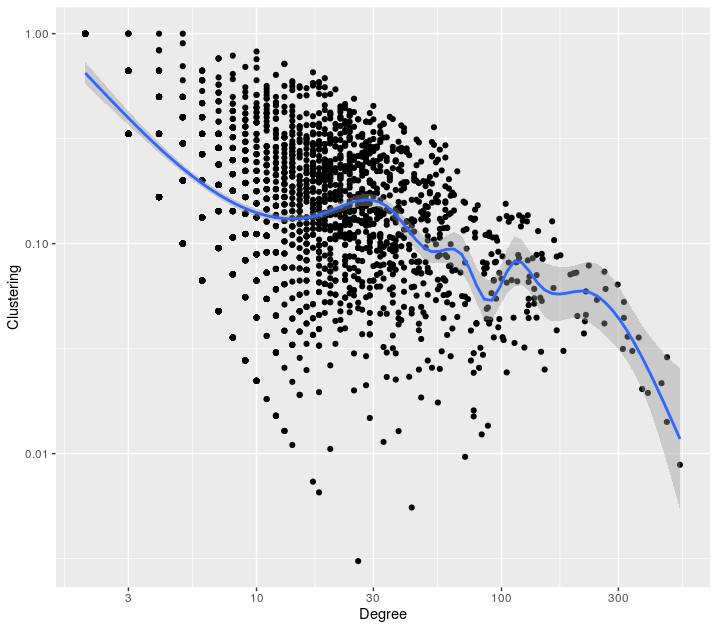
\includegraphics[width=\linewidth]{Rplot_transitivity_degree}
%  \caption{Local clustering coefficient and degree}
%  \label{fig:transitivity_degree}
%\end{figure}


%\begin{figure}
%    \centering
%    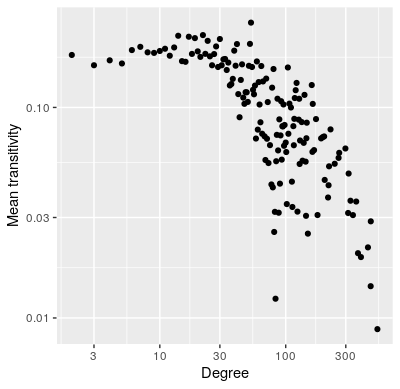
\includegraphics[width=\linewidth]{images/Rplot01_logdegree_log_transitivity.png}
%    \caption{Plot of degree with mean local transitivity. Log10-log10 scale. Omitting degree $k=1$ as transitivity $C$ will be undefined.}
 %   \label{fig:log_transitivity_degree}
%\end{figure}

\subsection{Results of disease enrichment for centrality measures}

Using the package disgennet2r disease enrichment was performed using the curated disgennet database using fishers exact test with FDR correction for multiple comparisons. 9703 genes were used as the background being those genes with annotated disease associations (not specifically synaptic)
\subsubsection{Degree}

Low degree (bottom 10\%) ataxia and seizures cut off 0.05

\begin{figure}
    \centering
    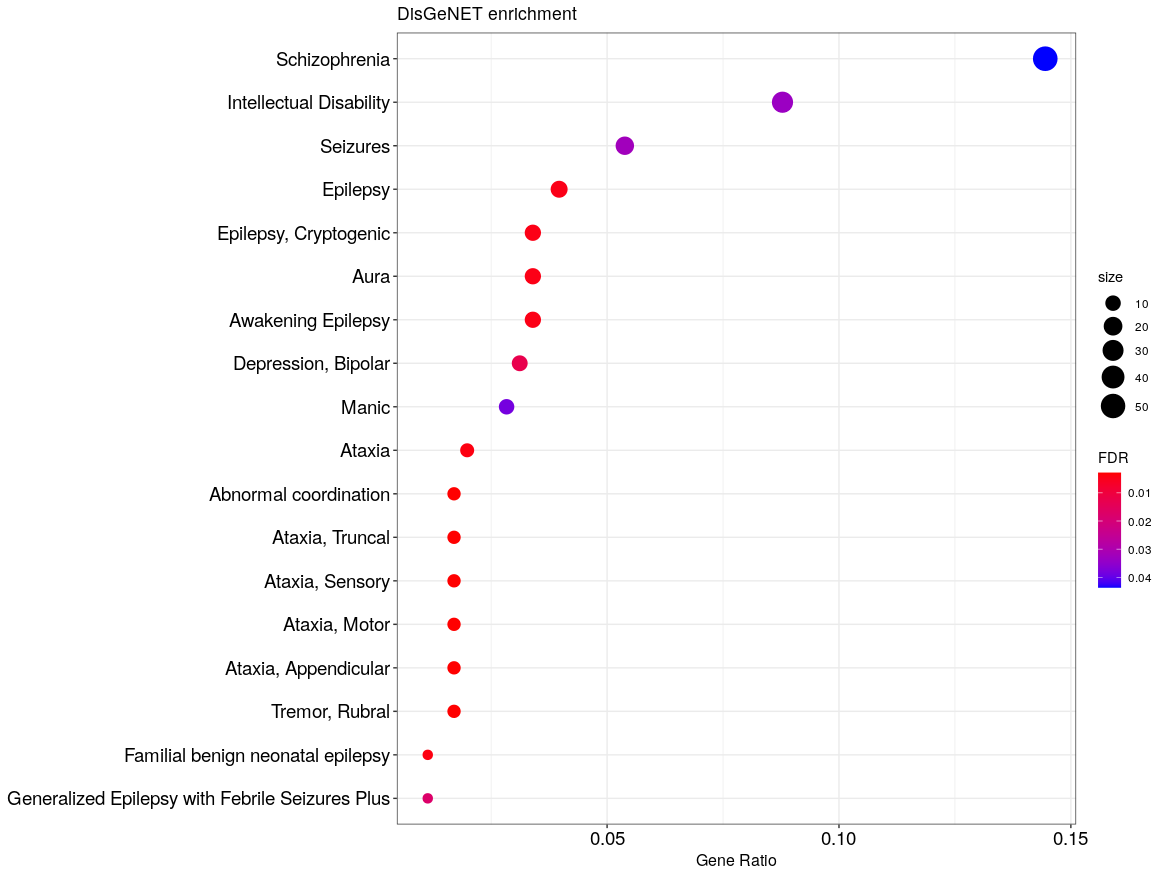
\includegraphics[width=\textwidth]{images/Rplot_low_deg_0.05cutoff_0.1cent_disgen.png}
    \caption{Low degree disease enrichment}
    \label{fig:low degree disease enrichment cut off 0.05}
\end{figure}


\begin{figure}
    \centering
    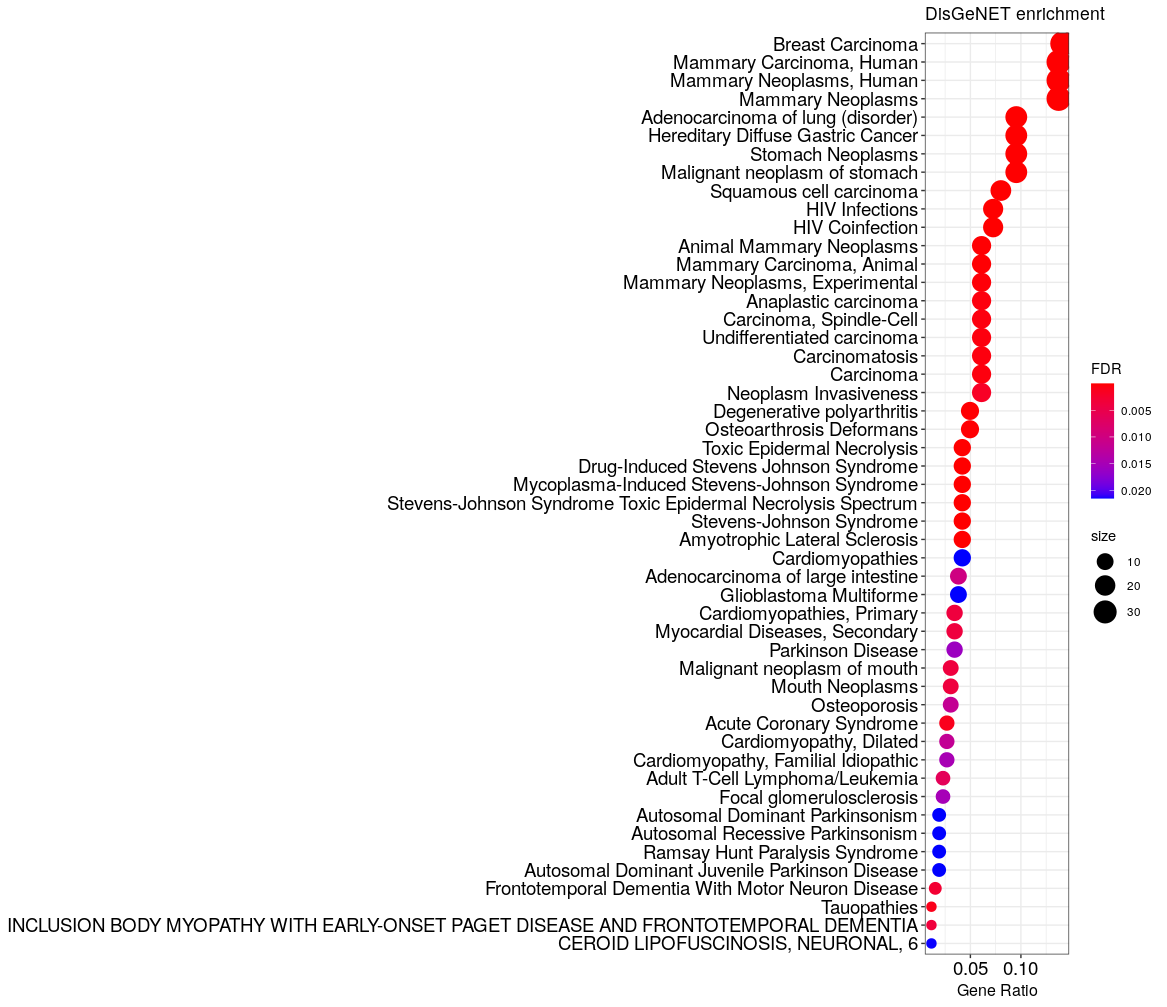
\includegraphics[width=\textwidth]{images/Rplot_high_deg_0.9_0.05cutoff_disgen.png}
    \caption{High degree disease enrichment}
    \label{fig:High degree disease enrichment cut off 0.05}
\end{figure}
Low degree includes a number of epilepsy (figure~\ref{fig:low degree disease enrichment cut off 0.05}). High degree (greater than 0.9 centile) enriches for neurological conditions ALS and Parkinson's disease (figure~\ref{fig:low degree disease enrichment cut off 0.05}).


Code \url{source('~/RProjects/graph2community/R/disgen3_degree_hi.R')}
\subsubsection{betweennness}

Diseases associated with high betweenness centrality were predominantly neoplasms showing those above the 90th centile for betweenness 0.0001121076, those in the bottom 10\% ($8.3 \times 10^{-5}$) were predominantly neurological disorders.

This suggests that highly central nodes are either not compatible with viability or are only affected in severely disordered pathology affecting essential cell functions such as tumours. 



\begin{figure}
    \centering
    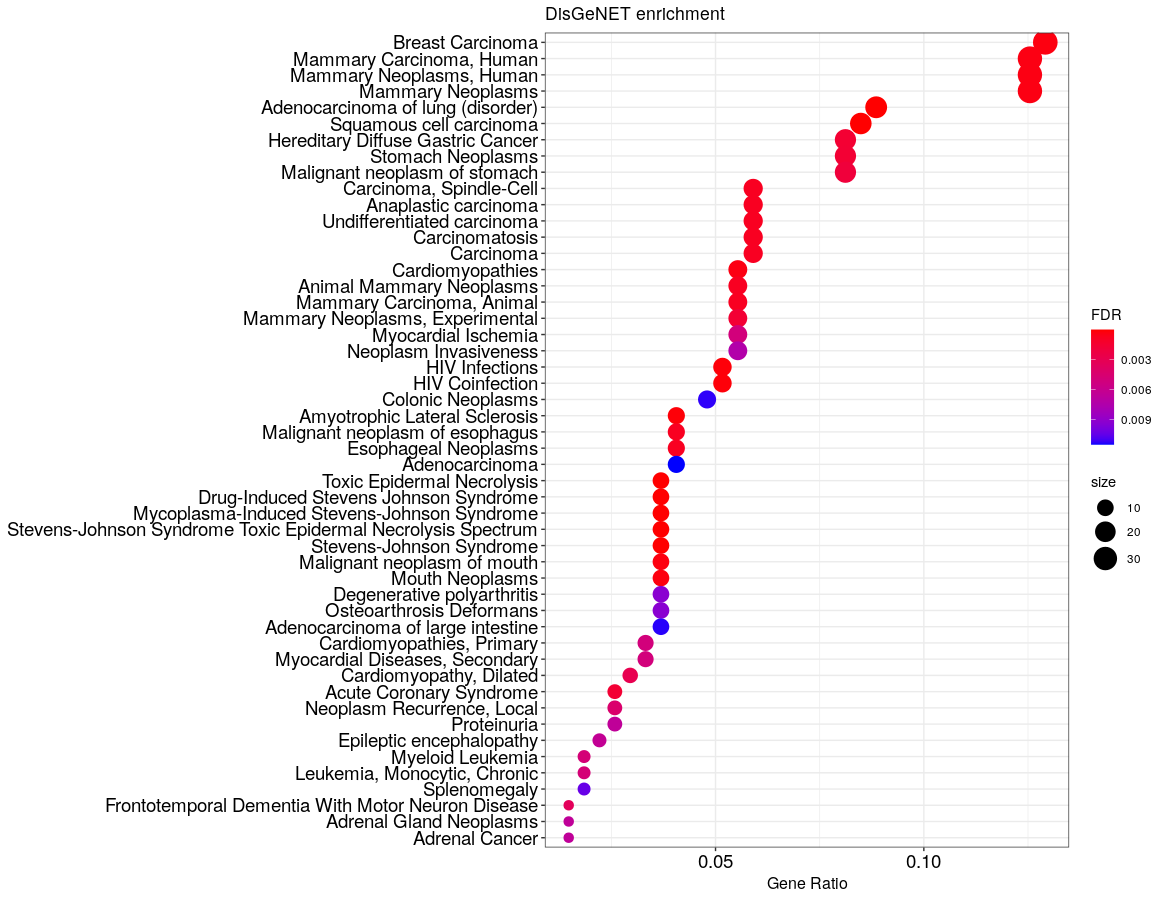
\includegraphics[width=\textwidth]{images/Rplot_high_bet_disgen.png}
    \caption{High betweenness nodes disease enrichment}
    \label{fig:high betweenness disease enrichment}
\end{figure}

\begin{figure}
    \centering
    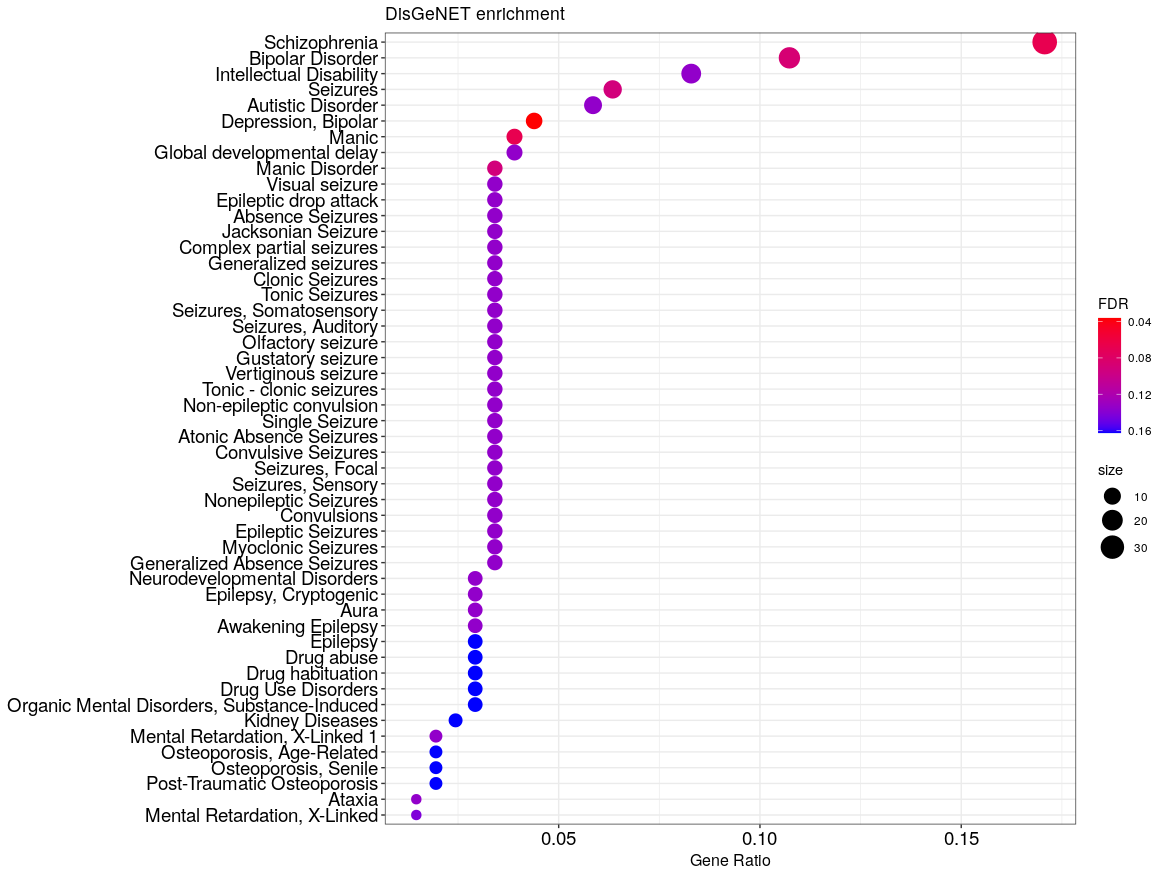
\includegraphics[width=\textwidth]{images/Rplot_bet_low0.1.png}
    \caption{Low betweenness disease enrichment}
    \label{fig:low betweenness disease enrichment}
\end{figure}



\subsubsection{Closeness centrality}



\begin{figure}
    \centering
    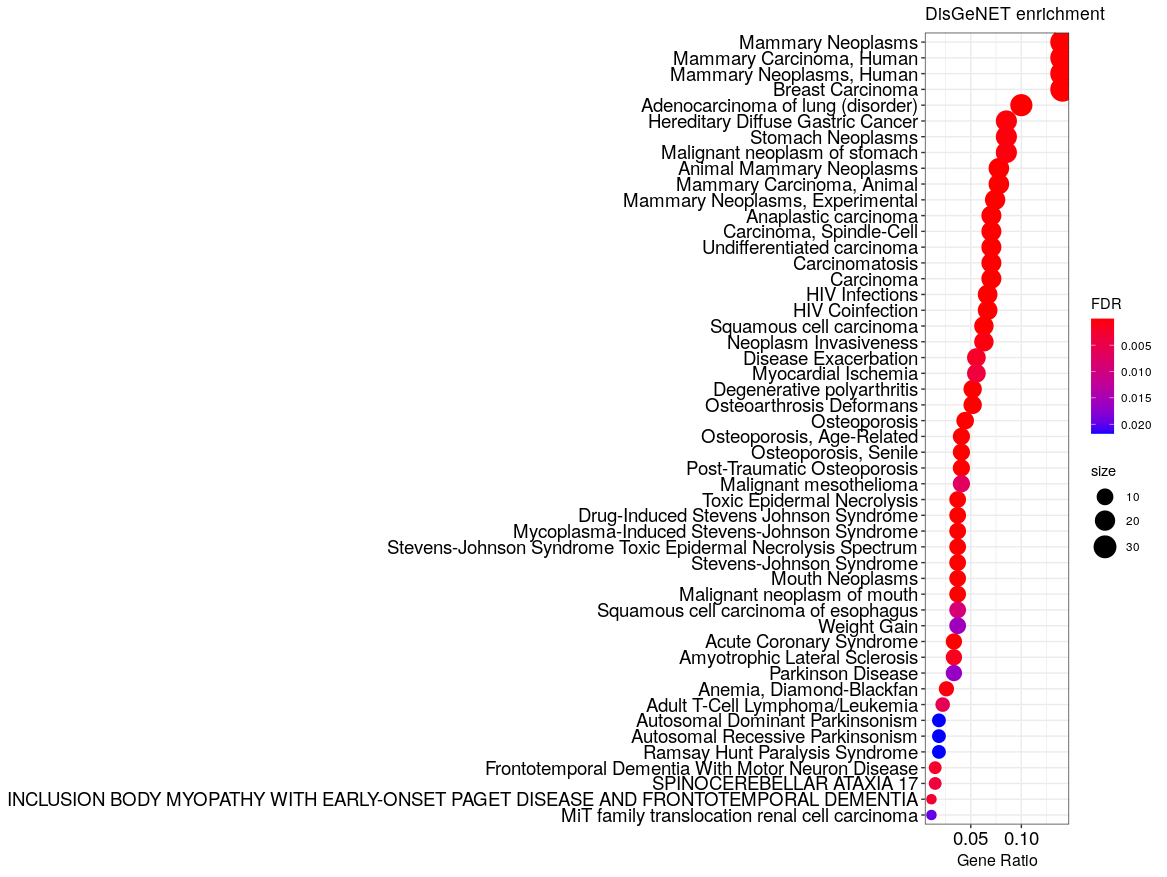
\includegraphics[width=\textwidth]{images/Rplot_high_closeness.png}
    \caption{High closeness disease enrichment}
    \label{fig:high closeness disease enrichment}
\end{figure}

\begin{figure}
    \centering
    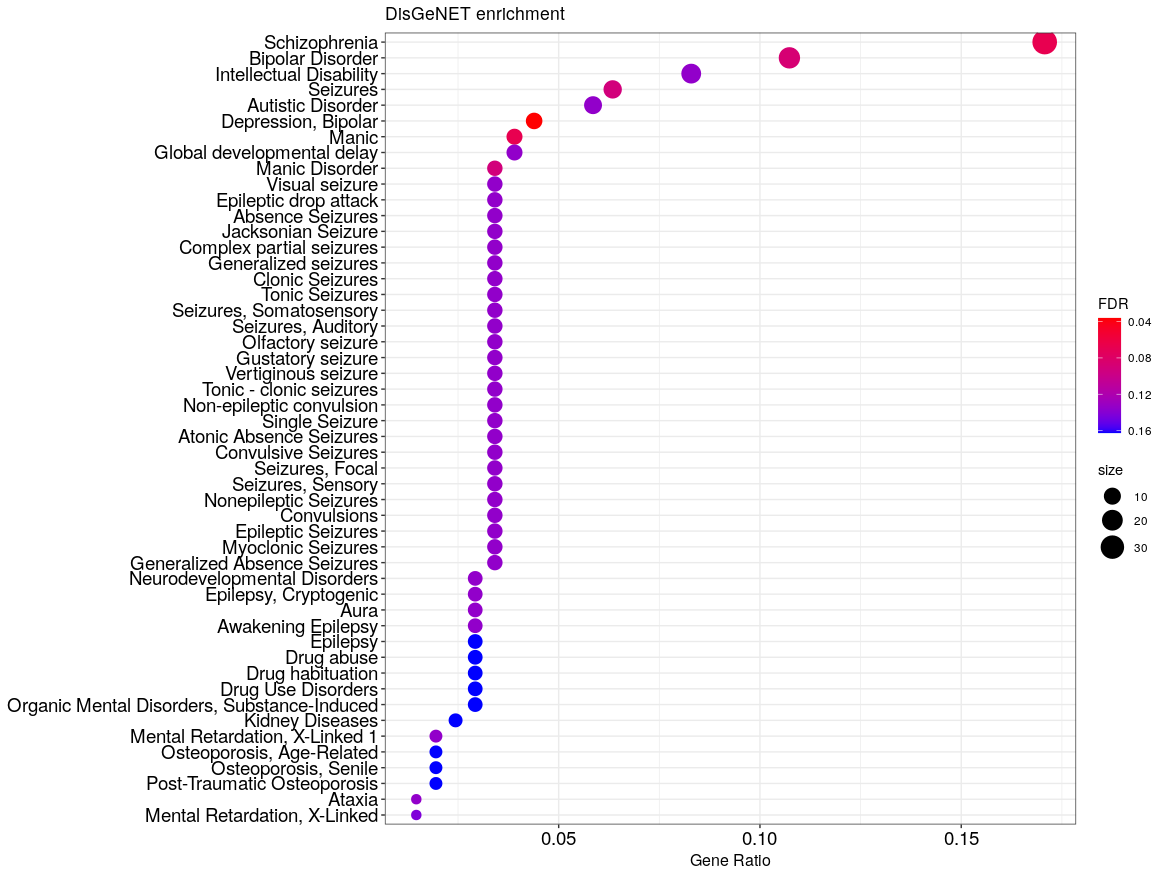
\includegraphics[width=\textwidth]{images/Rplot_low_closeness.png}
    \caption{Low closeness disease enrichment}
    \label{fig:low closeness disease enrichment}
\end{figure}



Note that the neurological conditions that are present with high closeness centrality are parkinsonism and some neurodegeneration


\subsubsection{Eigenvector centrality}

Parkinsons disease is again the highest ranking neurological disease in high eirgenvector centrality enrichment

40 low eigenvector annotated (greater than 0.9 centile)

261 high eigenvector centrality annotated (less than 0.1)


DisGeNet Low eigenvector centrality (figure~\ref{fig:low eigenvector disease enrichment cut off 0.05}.

Gene Ratio is number of terms from gene set in annotation over size of annotation

\begin{figure}
    \centering
    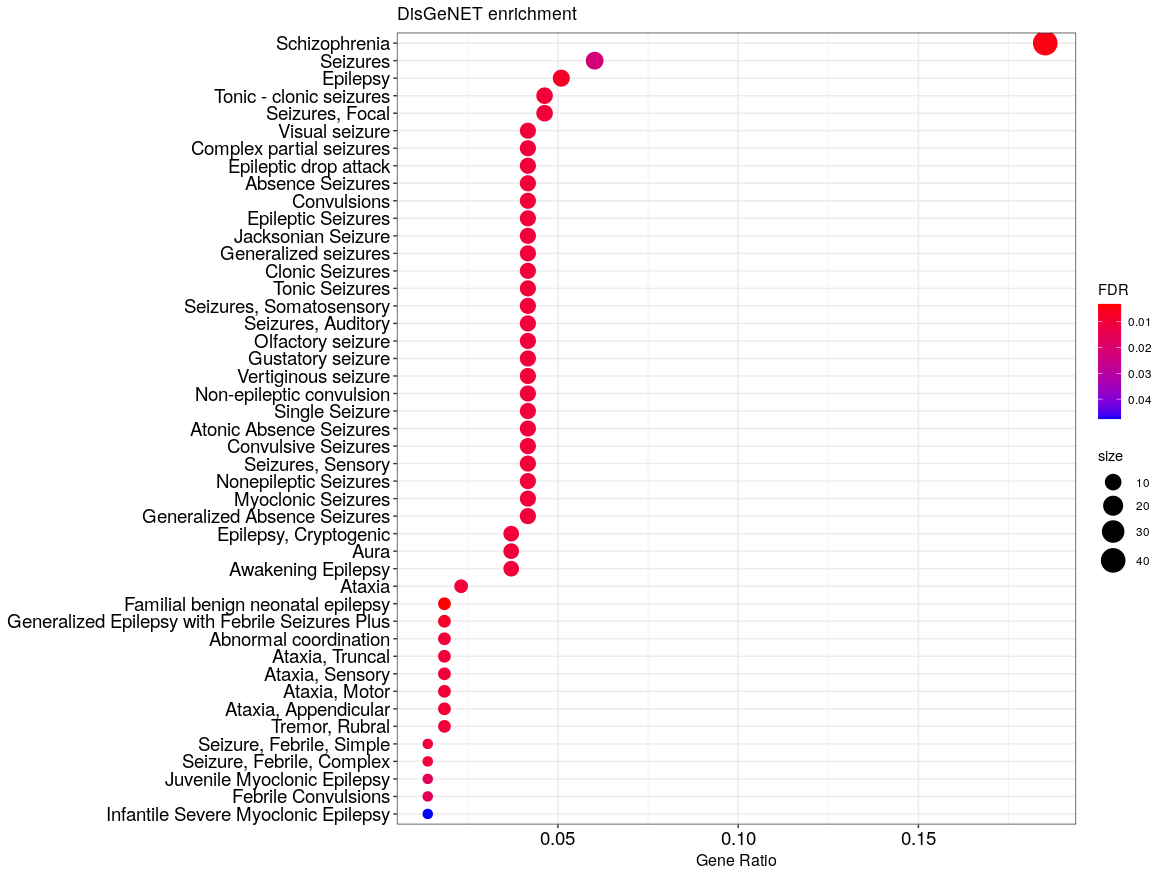
\includegraphics[width=\textwidth]{images/Rplot_low_eigenctror_centrality.png}
    \caption{Low eigenvector disease enrichment}
    \label{fig:low eigenvector disease enrichment cut off 0.05}
\end{figure}


\begin{figure}
    \centering
    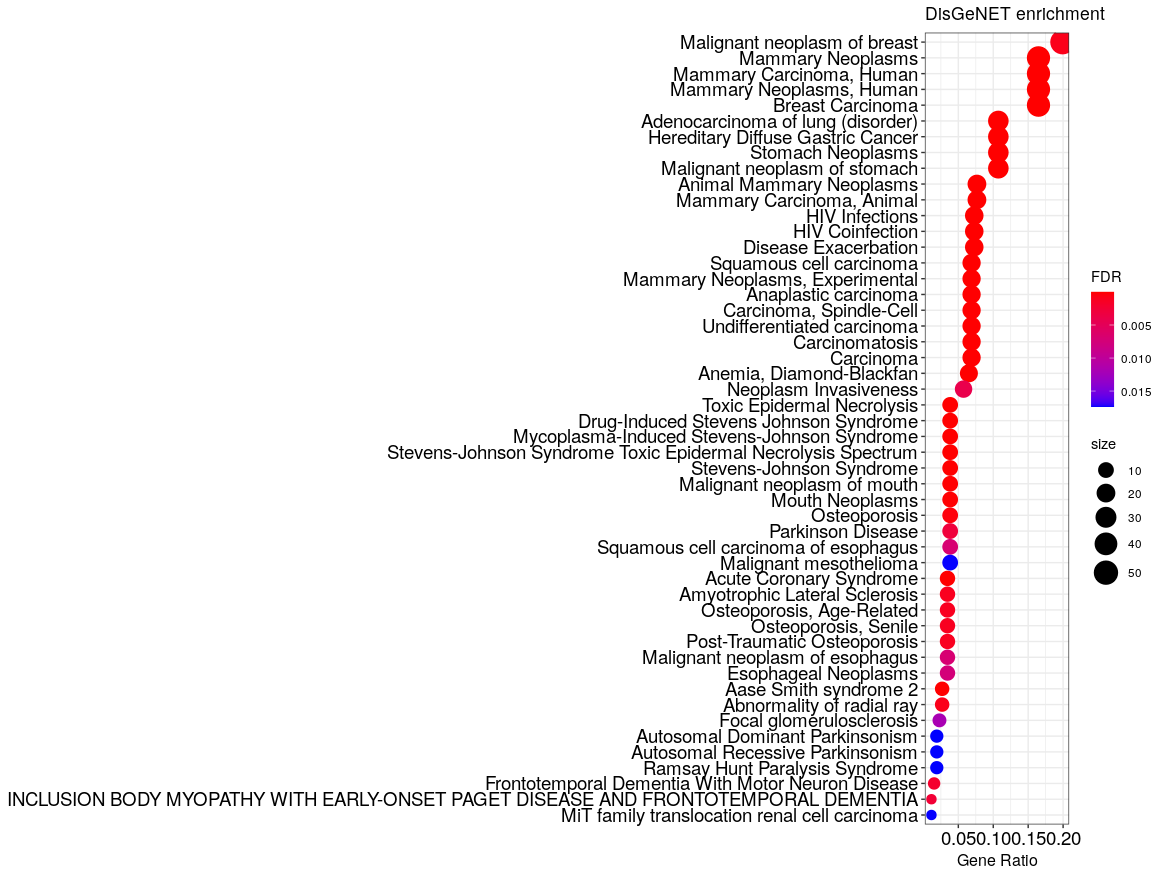
\includegraphics[width=\textwidth]{images/Rplot_high_eigenvector_centrality_disggen0.9].png}
    \caption{High eigenvector disease enrichment}
    \label{fig:high eigenvector disease enrichment cut off 0.05}
\end{figure}


\section{RESULTS: Centrality measures and graph statistics and Intelligence}

The correlation between the graph vertex centrality measures eigenvector centrality, betweenness centrality and transitivity and GWAS gene scores are shown in table \ref{Table:Correlation of GWAS gene level statistics with graph vertex measures}

The correlation between the graph vertex centrality measure statistics and the -log \textsubscript{10} transform of the vertex study p value is shown in table \ref{Table:Correlation of GWAS gene level statistics -log10 transform with graph vertex measures}

The Spearman rank correlation for -log\textsubscript{10} is shown in table \ref{Table:Correlation of GWAS gene level statistics Spearmans rho -log10 transform with graph vertex measures} and the rank correlation for p value and vertex statistic is found in table \ref{Table:Correlation of GWAS gene level statistics Spearmans rho gene p  with graph vertex measures} \todo{change S to scientific notation}

The vertex statistics are not normally distributed \todo{test this} and so we prefer the Spearman's rho. the -log\textsubscript{10} has the same value as $-\rho$ for p (signs switch).

\subsubsection{From paper moved here}
To test the hypothesis that genes encoding proteins with an important role in the structure of the PSP network were more likely to be associated with genetic variants associated with differences in intelligence or educational attainment (such as hubs), we calculated node degree, and four other measures of vertex importance: eigenvector centrality, betweenness centrality, closeness centrality and transitivity for each graph vertex (gene) using igraph. \cite{csardi2006igraph} \textcolor{red}{we need to say what all of these are before we start talking about them}\footnote{something like we will first of all need to introduce in general terms these measures and how they were calculated. in general also want to move more of this chapter into methods and results}. There was no correlation between any of these measures of vertex importance and their gene association analysis gene level statistics calculated using MAGMA (Spearman’s $\rho$ calculated with R) for genes in the post synaptic proteome graph. The results are presented in table 1\todo{table}. The complete vertex statistics for each PSP gene can be found in the supplementary material. 
\todo{Add multiple testing correction}


 \subsection{k coreness and GWAS results}
I also calculate the correlation between p and the coreness value of the vertex which is its k core \todo{expand}. There was no significant correlation as shown in table \ref{Table:Correlation of GWAS gene level statistics Spearmans rho gene p  with kcorecoreness measures}

%Code to complete this table is found at STRONTIUM\url{source('~/RProjects/paper_xls_output/R/make_df_graph_stats_correlation_PhDlatex.R')}.
\todo{fixed now}
% latex table generated in R 3.6.2 by xtable 1.8-4 package
% Sat Jan 11 12:31:46 2020
\begin{table}[ht]
\centering
\begin{adjustbox}{max width=\textwidth}
\begin{tabular}{rllrlrrrrl}
  \hline
 & Study & Graph statistic & t & df & p & cor & CI lower & CI upper & Test \\ 
  \hline
1 & Intelligence Discovery & Degree & 0.75 & 3299 & 0.45 & 0.01 & -0.02 & 0.05 & Pearson's product-moment correlation \\ 
  2 & Intelligence Discovery & Betweenness & 0.12 & 3299 & 0.90 & 0.00 & -0.03 & 0.04 & Pearson's product-moment correlation \\ 
  3 & Intelligence Discovery & Eigenvector & 0.73 & 3299 & 0.47 & 0.01 & -0.02 & 0.05 & Pearson's product-moment correlation \\ 
  4 & Intelligence Discovery & Transitivity & -0.94 & 3012 & 0.35 & -0.02 & -0.05 & 0.02 & Pearson's product-moment correlation \\ 
  5 & Intelligence Replication & Degree & -0.64 & 3307 & 0.52 & -0.01 & -0.04 & 0.02 & Pearson's product-moment correlation \\ 
  6 & Intelligence Replication & Betweenness & -0.38 & 3307 & 0.71 & -0.01 & -0.04 & 0.03 & Pearson's product-moment correlation \\ 
  7 & Intelligence Replication & Eigenvector & -0.33 & 3307 & 0.74 & -0.01 & -0.04 & 0.03 & Pearson's product-moment correlation \\ 
  8 & Intelligence Replication & Transitivity & 1.00 & 3019 & 0.31 & 0.02 & -0.02 & 0.05 & Pearson's product-moment correlation \\ 
  9 & Education Discovery & Degree & -0.25 & 3299 & 0.80 & -0.00 & -0.04 & 0.03 & Pearson's product-moment correlation \\ 
  10 & Education Discovery & Betweenness & -1.10 & 3299 & 0.29 & -0.02 & -0.05 & 0.02 & Pearson's product-moment correlation \\ 
  11 & Education Discovery & Eigenvector & 1.00 & 3299 & 0.32 & 0.02 & -0.02 & 0.05 & Pearson's product-moment correlation \\ 
  12 & Education Discovery & Transitivity & 0.09 & 3012 & 0.93 & 0.00 & -0.03 & 0.04 & Pearson's product-moment correlation \\ 
  13 & Education Replication & Degree & -1.20 & 3283 & 0.23 & -0.02 & -0.06 & 0.01 & Pearson's product-moment correlation \\ 
  14 & Education Replication & Betweenness & -0.63 & 3283 & 0.53 & -0.01 & -0.04 & 0.02 & Pearson's product-moment correlation \\ 
  15 & Education Replication & Eigenvector & -0.45 & 3283 & 0.65 & -0.01 & -0.04 & 0.03 & Pearson's product-moment correlation \\ 
  16 & Education Replication & Transitivity & 1.50 & 2998 & 0.14 & 0.03 & -0.01 & 0.06 & Pearson's product-moment correlation \\ 
   \hline
\end{tabular}
\end{adjustbox}
\caption{Correlation of GWAS gene level statistics with graph vertex measures.Code to complete this table is found at STRONTIUM\url{source('~/RProjects/paper_xls_output/R/make_df_graph_stats_correlation_PhDlatex.R')}}
\label{Table:Correlation of GWAS gene level statistics with graph vertex measures}
\end{table}

% latex table generated in R 3.6.2 by xtable 1.8-4 package
% Sat Jan 11 12:43:57 2020
\begin{table}[ht]
\centering
  \begin{adjustbox}{max width=\textwidth}
\begin{tabular}{rllrlrrrrl}
  \hline

 & Study & Graph statistic & t & df & p & cor & confidence\_int\_lower & condidence\_upper & Test \\ 
  \hline
1 & Intelligence Discovery & Degree & -0.40 & 3299 & 0.69 & -0.01 & -0.04 & 0.03 & Pearson's product-moment correlation \\ 
  2 & Intelligence Discovery & Betweenness & 0.04 & 3299 & 0.97 & 0.00 & -0.03 & 0.04 & Pearson's product-moment correlation \\ 
  3 & Intelligence Discovery & Eigenvector & -0.31 & 3299 & 0.76 & -0.01 & -0.04 & 0.03 & Pearson's product-moment correlation \\ 
  4 & Intelligence Discovery & Transitivity & 0.59 & 3012 & 0.56 & 0.01 & -0.03 & 0.05 & Pearson's product-moment correlation \\ 
  5 & Intelligence Replication & Degree & -0.14 & 3307 & 0.89 & -0.00 & -0.04 & 0.03 & Pearson's product-moment correlation \\ 
  6 & Intelligence Replication & Betweenness & -0.41 & 3307 & 0.68 & -0.01 & -0.04 & 0.03 & Pearson's product-moment correlation \\ 
  7 & Intelligence Replication & Eigenvector & -0.51 & 3307 & 0.61 & -0.01 & -0.04 & 0.03 & Pearson's product-moment correlation \\ 
  8 & Intelligence Replication & Transitivity & -0.88 & 3019 & 0.38 & -0.02 & -0.05 & 0.02 & Pearson's product-moment correlation \\ 
  9 & Education Discovery & Degree & -0.84 & 3299 & 0.40 & -0.01 & -0.05 & 0.02 & Pearson's product-moment correlation \\ 
  10 & Education Discovery & Betweenness & -0.55 & 3299 & 0.58 & -0.01 & -0.04 & 0.03 & Pearson's product-moment correlation \\ 
  11 & Education Discovery & Eigenvector & -1.70 & 3299 & 0.08 & -0.03 & -0.06 & 0.00 & Pearson's product-moment correlation \\ 
  12 & Education Discovery & Transitivity & 0.74 & 3012 & 0.46 & 0.01 & -0.02 & 0.05 & Pearson's product-moment correlation \\ 
  13 & Education Replication & Degree & 1.10 & 3283 & 0.29 & 0.02 & -0.02 & 0.05 & Pearson's product-moment correlation \\ 
  14 & Education Replication & Betweenness & 0.87 & 3283 & 0.38 & 0.01 & -0.02 & 0.05 & Pearson's product-moment correlation \\ 
  15 & Education Replication & Eigenvector & -0.05 & 3283 & 0.96 & -0.00 & -0.04 & 0.03 & Pearson's product-moment correlation \\ 
  16 & Education Replication & Transitivity & -2.00 & 2998 & 0.04 & -0.04 & -0.07 & -0.00 & Pearson's product-moment correlation \\ 
   \hline
\end{tabular}
\end{adjustbox}
\caption{Correlation of GWAS gene level statistics -log10 transform with graph vertex measures} 
\label{Table:Correlation of GWAS gene level statistics -log10 transform with graph vertex measures}
\end{table}


% latex table generated in R 3.6.2 by xtable 1.8-4 package
% Sat Jan 11 12:58:15 2020
\begin{table}[ht]
\centering
  \begin{adjustbox}{max width=\textwidth}
\begin{tabular}{rllrrrl}
  \hline
 & Study & Graph statistic & S & p & rho & Test \\ 
  \hline
1 & Intelligence Discovery & Degree & 6200000000.00 & 0.04 & -0.04 & Spearman's rank correlation rho \\ 
  2 & Intelligence Discovery & Betweenness & 6200000000.00 & 0.05 & -0.03 & Spearman's rank correlation rho \\ 
  3 & Intelligence Discovery & Eigenvector & 6200000000.00 & 0.11 & -0.03 & Spearman's rank correlation rho \\ 
  4 & Intelligence Discovery & Transitivity & 4500000000.00 & 0.85 & 0.00 & Spearman's rank correlation rho \\ 
  5 & Intelligence Replication & Degree & 5900000000.00 & 0.20 & 0.02 & Spearman's rank correlation rho \\ 
  6 & Intelligence Replication & Betweenness & 5900000000.00 & 0.21 & 0.02 & Spearman's rank correlation rho \\ 
  7 & Intelligence Replication & Eigenvector & 6000000000.00 & 0.93 & -0.00 & Spearman's rank correlation rho \\ 
  8 & Intelligence Replication & Transitivity & 4700000000.00 & 0.34 & -0.02 & Spearman's rank correlation rho \\ 
  9 & Education Discovery & Degree & 6000000000.00 & 0.69 & -0.01 & Spearman's rank correlation rho \\ 
  10 & Education Discovery & Betweenness & 6000000000.00 & 0.92 & -0.00 & Spearman's rank correlation rho \\ 
  11 & Education Discovery & Eigenvector & 6200000000.00 & 0.07 & -0.03 & Spearman's rank correlation rho \\ 
  12 & Education Discovery & Transitivity & 4600000000.00 & 0.77 & -0.01 & Spearman's rank correlation rho \\ 
  13 & Education Replication & Degree & 5800000000.00 & 0.53 & 0.01 & Spearman's rank correlation rho \\ 
  14 & Education Replication & Betweenness & 5800000000.00 & 0.39 & 0.01 & Spearman's rank correlation rho \\ 
  15 & Education Replication & Eigenvector & 6000000000.00 & 0.65 & -0.01 & Spearman's rank correlation rho \\ 
  16 & Education Replication & Transitivity & 4600000000.00 & 0.10 & -0.03 & Spearman's rank correlation rho \\ 
   \hline
\end{tabular}
\end{adjustbox}
\caption{Correlation of GWAS gene level statistics Spearmans rho -log10 transform with graph vertex measures \url{source('~/RProjects/paper_xls_output/R/make_df_graph_stats_correlation_spearman_log10_PhDlatex.R')}} 
\label{Table:Correlation of GWAS gene level statistics Spearmans rho -log10 transform with graph vertex measures}
\end{table}

% latex table generated in R 3.6.2 by xtable 1.8-4 package
% Sat Jan 11 13:06:00 2020
\begin{table}[ht]
\centering
  \begin{adjustbox}{max width=\textwidth}
\begin{tabular}{rllrrrl}
  \hline
 & Study & Graph statistic & S & p & rho & Test \\ 
  \hline
1 & Intelligence Discovery & Degree & 5800000000.00 & 0.04 & 0.04 & Spearman's rank correlation rho \\ 
  2 & Intelligence Discovery & Betweenness & 5800000000.00 & 0.05 & 0.03 & Spearman's rank correlation rho \\ 
  3 & Intelligence Discovery & Eigenvector & 5800000000.00 & 0.11 & 0.03 & Spearman's rank correlation rho \\ 
  4 & Intelligence Discovery & Transitivity & 4600000000.00 & 0.85 & -0.00 & Spearman's rank correlation rho \\ 
  5 & Intelligence Replication & Degree & 6200000000.00 & 0.20 & -0.02 & Spearman's rank correlation rho \\ 
  6 & Intelligence Replication & Betweenness & 6200000000.00 & 0.21 & -0.02 & Spearman's rank correlation rho \\ 
  7 & Intelligence Replication & Eigenvector & 6000000000.00 & 0.93 & 0.00 & Spearman's rank correlation rho \\ 
  8 & Intelligence Replication & Transitivity & 4500000000.00 & 0.34 & 0.02 & Spearman's rank correlation rho \\ 
  9 & Education Discovery & Degree & 6000000000.00 & 0.69 & 0.01 & Spearman's rank correlation rho \\ 
  10 & Education Discovery & Betweenness & 6000000000.00 & 0.92 & 0.00 & Spearman's rank correlation rho \\ 
  11 & Education Discovery & Eigenvector & 5800000000.00 & 0.07 & 0.03 & Spearman's rank correlation rho \\ 
  12 & Education Discovery & Transitivity & 4500000000.00 & 0.77 & 0.01 & Spearman's rank correlation rho \\ 
  13 & Education Replication & Degree & 6000000000.00 & 0.53 & -0.01 & Spearman's rank correlation rho \\ 
  14 & Education Replication & Betweenness & 6000000000.00 & 0.39 & -0.01 & Spearman's rank correlation rho \\ 
  15 & Education Replication & Eigenvector & 5900000000.00 & 0.65 & 0.01 & Spearman's rank correlation rho \\ 
  16 & Education Replication & Transitivity & 4400000000.00 & 0.10 & 0.03 & Spearman's rank correlation rho \\ 
   \hline
\end{tabular}
  \end{adjustbox}
\caption{Correlation of GWAS gene level statistics Spearmans rho gene p with graph vertex measures \url{source('~/RProjects/paper_xls_output/R/make_df_graph_stats_correlation_spearman_P_PhDlatex.R')}} 
\label{Table:Correlation of GWAS gene level statistics Spearmans rho gene p  with graph vertex measures}
\end{table}

% latex table generated in R 3.6.2 by xtable 1.8-4 package
% Sat Jan 11 13:27:32 2020
\begin{table}[ht]
\centering
  \begin{adjustbox}{max width=\textwidth}
\begin{tabular}{rllrrrl}
  \hline
 & Study & Graph statistic & S & p & rho & Test \\ 
  \hline
5 & Intelligence Discovery & Coreness & 5800000000.00 & 0.07 & 0.03 & Spearman's rank correlation rho \\ 
  10 & Intelligence Replication & Coreness & 6200000000.00 & 0.27 & -0.02 & Spearman's rank correlation rho \\ 
  15 & Education Discovery & Coreness & 5900000000.00 & 0.52 & 0.01 & Spearman's rank correlation rho \\ 
  20 & Education Replication & Coreness & 5900000000.00 & 0.79 & -0.00 & Spearman's rank correlation rho \\ 
   \hline
\end{tabular}
\end{adjustbox}
\caption{Correlation of GWAS gene level statistics Spearmans rho gene p with kcore coreness measures \url{source('~/RProjects/paper_xls_output/R/make_df_graph_stats_correlation_spearman_P_kcore_PhDlatex.R')}} 
\label{Table:Correlation of GWAS gene level statistics Spearmans rho gene p  with kcorecoreness measures}
\end{table}






\subsection{Results Centrality and murine models of long term potentiation}
\label{sec:results centrality and murine models of long term potentiation}
    The centrality measures of genes marked as murine models of LTP were considered as model animal models of intelligence. \footnote{\url{source('~/RProjects/centrality/R/model_ltp/model ltp.R')}}.
    256 genes were identified as a
    ssociated with murine LTD from \textcolor{red}{add Mouse ontology}\todo{add mouse ontology}. 141 of these genes were found in the PSP network model (55.1\%).
    
    There was no statistically significant difference in association between the centrality measures of those genes associated with LTP and the rest of the PSP. Tested degree (0.809), eigenvector centrality (0.630), betweenness (0.895) and transitivity (0.898) Wilcoxon rank sum test with continuity correction. 
    
    A logistic regression model of these factors and LTP PSP as outcome showed that eigenvector centrality and degree were significant factors (4.04 $\times 10^{-6}$ and $1.39 \times 10^{-6}$. The effects were very minor however with McFadden's pseudo R2 \cite{mcfadden1973conditional} calculated using the pscl package was  0.031 \cite{jackman2017package}.

\subsubsection{Other notes}

enrichment of genes found in the synapse with orthologs in yeast reveal a large number for exosome and mitochondrial elements
\textbf{Articulation points}
11 of 68 glutamate receptor binding are articulation points however Gene ontology enrichment analysis ofarticulation points with the entire PSP as background yileds no significant over-representation of terms. They appear to be under represented in ID (3 genes of 203.	 	
\section{Summary}

We show that in the PSP nodes of very high centrality are associated with essentialness. The PSP has a high degree of essentialness compared to the rest of the genome. 

High degree nodes are associated with specific phenotypes and specific gene ontology terms however the are not correlated with genetic differences that are enriched for differences in intelligence. This is not obvious before the fact and is different from other traits eg essentialness. One might hypothesis that the reason is that there is either no effect (ie it is irrelevant) or that in population studies genes with high centrality are more likely to be essential and hence have less genetic variation. We find also in one of the principle animal models of learning murine long term potentiation that genes of high importance were no more likely or less likely to be involved in long term potentiation.

We use data from the Exac project to further investigate whether high importance nodes were subject to selection pressure such that they proved more intolerant of non synonymous genetic changes. Nodes with high degree are associated with an increased probability of being intolerant to changes. 

Nodes with high betweenness centrality were involved in neuro-degenerative disorders including Parkinson's disease see section~\ref{sec:Betweeness centrality}. They were also associated with severe phenotypes in murine models including phenotypes incompatibly with viability. Low betweenness centrality was associated with abnormalities in synaptic transmission in murine models. 

High eigenvector centrality is again associated with severe murine phenotypes and enrichment for RNA and cadherin binding. Disease enrichment is of neoplasms and neurodegenerative disorders. 

Low eigenvector centrality (10\%) were enriched for human phenotypes of seizures and ontology terms of transmitter, mouse phenotype was of abnormal synaptic transmission. The top five enriched disorders in disGeNET were seizure related. 

Despite this there was no association between node centrality measures and the significance of genetic variants for differences in intelligence and educational attainment.

There is a complex relationship between transitivity and degree for nodes with degree 3 or less the correlation is positive and results in a positive overall correlation despite a plot of the relationship appearing clearly negative. This is due to the large number of low degree nodes. When the correlation is calculated for higher degree the relationship previously commented upon in the literature \cite{newman} p 335 is seen. Caution should therefore be used in determining linear correlations involving transitivity especially in smaller networks and it may be prudent to plot the correlation against minimum degree.


 
\section{General to dos}

Table of diameters \cite{crescenzi2013computing}
 table 4 
 \todo{enrichment of high/low scoring groups of genes}
 \todo{add intellectual disability graph measures or indeed other disorders from toppgene}
 \todo{define configuration model}
 \todo{plot of distribution of other centrality measures}
\todo{centrality measures for significant genes}
\todo{centralisation 1:09 in zhukov - centrality is how central most central node is compared to other nodes in graph, max with star network}
\todo{Metrics comparison zhukov at 1:15}
%Scatter plot of centralities multiplot eg plot(bet,deg) DONE

Kendal tau rank - concordant pairs ie a comes before b in both samples 

most recent centrality in \url{source('~/RProjects/centrality/R/other_centrality/eccentricity_and_distance.R')}


\section{Value of tissue specific networks}
\cite{parikshak2015systems} quotes the example of cardiac PPI to investigaste long QT in \cite{lundby2014annotation}

Kitsak and Barabasi \cite{kitsak2016tissue}



%\chapter{Find place}



This chapter at present contains those bits that don't quite fit in where they are

\section{Ideas}

Add a chapter called confirming our findings. After reading Plomin EA3 and Savage are the largest educational attainment and intelligence cohorts. We should therefore validate our findings from the discovery (Discovery and Replication cohort) in these eg enrichment for different phenotypes, subgroup analysis, orthologues, core periphery etc. We don't have access to solely the bits that are new but we can say that our findings hold up for the largest population studies to date including the largest amount of variance. Also add exomes to discussion under future work. 

Sample from neurogenesis gene ontology for sizes similar to our groups and also see if enriched for other cohorts eg Savage
add this to simulation p levels too. 

\section{Orthologs Keith}
\textcolor{red}{from centrality}
See code % RProjects/orthologs mac

from bit with Keith remove ph. See table \ref{tab:orthologs_pseudospokes}
\begin{table}[ht]
\centering
\begin{tabular}{rlrrrrl}
  \hline
 & species & data\_PSP & data\_ps & ratio\_PSP\_human & ratio\_ps\_human & p post hoc \\ 
  \hline
1 & human & 3457 & 104 & 1.00 & 1.00 & NA (test) \\ 
  2 & mouse & 3351 & 103 & 0.97 & 0.99 & 0.93 \\ 
  3 & worm & 2180 &  73 & 0.63 & 0.70 & 0.054 \\
  4 & zebra fish & 2342 &  80 & 0.68 & 0.77 &0.443\\ 
  5 & yeast & 835 &  49 & 0.24 & 0.47 &0.000195*** \\ 
  6 & fly & 1923 &  68 & 0.56 & 0.65 &0.3\\ 
   \hline
\end{tabular}
\caption{Presence of orthologs in PSP and amongst pseudohubs. Ratio of number of orthologs to human genes in PSP and pseudohubs. There are a significant excess of yeast orthologs in this group.Pearson's Chi square test pseudospokes ortholog frequency X-squared = 16.841, df =5 , p-value = 0.0048, $\alpha$ bonferroni=0.01.}
\label{tab:orthologs_pseudospokes}
\end{table}

\subsection{More orthologs}
\textcolor{red}{from centrality}
gmt for orthologs on MAC is at \url{ukbbedortholog_PSP.gmt.sets.out }

Core and periphery
and add ontology groups



\section{DIAMonD algo}

On initial testing and on redo the dianmond algorithm does no better than chance the first I think is using my network as I find a shell script in a pycharm project on the mac called diamond).

Basically works no better than chance on either PSD network or supplied network (although some not found (need to include))

Here are the warnings

\footnote{DIAMOnD(): ignoring 5 of 47 seed genes that are not in the network

 results have been saved to 'ctg\_predict.txt' 

DIAMOnD(): ignoring 15 of 99 seed genes that are not in the network

 results have been saved to 'ea2\_predict.txt' 

DIAMOnD(): ignoring 37 of 196 seed genes that are not in the network

 results have been saved to 'ukbb\_int\_predict.txt' 

DIAMOnD(): ignoring 43 of 235 seed genes that are not in the network

 results have been saved to 'ukbbed.txt' }

\subsection{Testing the algorithm}
 Using 200 predictions from CTG 1 match found in ukbbint and 4 in ukbbed
 from EA2 1 match in ukbbint and 4 in ukbbed
 No matches in any other phenotype using ukbbed and ukbbint seed lists.
 \begin{table}[ht]
\centering
\begin{tabular}{rll}
  \hline
  SET & n in synapse & total significant\\ 
  \hline
 CTG & 16 &47\\
 EA2 & 25 & 98\\
 UKBBint & 49 & 193\\
  UKBBEd & 56 & 232\\
  \\ 
 
   \hline
\end{tabular}
\caption{Significant synaptic genes}
\label{table:MAGMA_Gene_result_significant synaptic genes}
\end{table}

 No matches in any other phenotype using ukbbed and ukbbint seed lists.
 \begin{table}[ht]
\centering
\begin{tabular}{lrlll}
  \hline
  &CTG & EA2 &UKBBint & UKBBed t\\ 
  \hline
 CTG & 16 &1 & \textbf{10}& 6\\
 EA2 & 1 & 25 & 11 & \textbf{25}\\
 UKBBint &\textbf{10}  & 11 & 49 & 18\\
  UKBBEd & 6  & \textbf{25} & 18 & 56\\
  \\ 
 
   \hline
\end{tabular}
\caption{Significant synaptic genes. Shared phenotype in bold. Diagnonal terms equals number of significant (genome wide for gene) genes in phenotype}
\label{table:MAGMA_Gene_result_significant neighbour overlap synaptic genes}
\end{table}
 
 The significant genes do not certainly form a cohesive network. The significant genes for UKBiobank Ed were in 52 components, 1 of size 2 and 1 of size 3 the rest were isolated. 
 
 UKBBInt 52 components 2 of size 2 and 1 of size 3.
 
 CTG 16 individual components
 
 EA2 25 individual components. 
 
 Therefore the significant genes do not form a connected group of any significant size.
 
 \todo{?in neighbours}
 
 CTG has 158 direct neighbours,ea2 has 327, ukbbed has 531 and ukbbint has 544
 
 Intersect ctg and ukbbint neighbours 119
 Intersect ctg and ukbbed 100
 Insersect ctg and ea2 62
 
 Intersect ea2 and ukbbint 168
 Intersect ea2 and ukbbed 250
 
 Intersect ukbbint and ukbbed 301
 
  \begin{table}[ht]
\centering
\begin{tabular}{lrlll}
  \hline
  &CTG & EA2 &UKBBint & UKBBed \\ 
  \hline
 CTG & 158 &62 & \textbf{119}& 100\\
 EA2 & 62 & 327 & 168 & \textbf{250}\\
 UKBBint &\textbf{119}  & 168 & 544 & 301\\
  UKBBEd & 100  & \textbf{25} & 301 & 531\\
  \hline
\end{tabular}
\caption{Significant synaptic genes neighbours overlap. Shared phenotype in bold. Diagonal terms equals number of significant (genome wide for gene) genes in phenotype}
\label{table:MAGMA_Gene_result_significant_synaptic_genes_neighbours_overlap}
\end{table}


 code: \url{('~/RProjects/PhD_graphs/R/induced_subgraph_gene_results_generic.R')}
 So for very basic simulation:
 %\url{RProjects\PhD_graphs\sample\subgraphs_GR.R}  
 Generate connected graphs of approximately the same size as the connected graph of neighbours (lookup average largest component size when random sampling from ids and extracting largest component)
 
 overlap size 158 and 327 expected value 17.59 see
 
%\url{RProjects\PhD_graphs\sample\subgraphs_GR.R}  

\url{RProjects}
actual  62
 
 UKBB size and UKBBEd size sample 750 expected overlap 103 sd 10.6 actual 301
 
 ctg and ukbbed (will be roughly same as ukbbint as n in these groups same)
 27.6 sd 7 (expected) actual ctg ukbbint 119 ukbbed 100
 
 ea2 and ukbb (int and ed as based on sampling and so size based (approx)
 
 ea2 n=327 neighbours so sample approx n=500
 
 Mean overlap EA2 and UKBB int and ed size connected groups 60.45 sd(7.5). Observed 168 (intelligence) and 250 (education)
 
 The significant genes belong to the same neighbourhood in the graph and this appears to be significant. We have shown that the significant genes do not form cohesive groups but that their 1 jump neighbours overlap more than expected by chance therefore they are more collocated in the graph than one would expect by chance.  I will need to decrease the step size in the sampling table below and increase the number of samples to approach exact numbers for each group and confidence intervals \todo{increase accuracy of sampling}
 
 
 Example of sampling table:
 
 % latex table generated in R 3.4.4 by xtable 1.8-4 package
% Wed Oct  9 17:21:05 2019
\begin{table}[ht]
\centering
\begin{tabular}{rrr}
  \hline
 & samples & mean\_n\_largest component \\ 
  \hline
1 & 200.00 & 70.27 \\ 
  2 & 250.00 & 106.14 \\ 
  3 & 300.00 & 144.47 \\ 
  4 & 350.00 & 187.09 \\ 
  5 & 400.00 & 229.26 \\ 
  6 & 450.00 & 274.06 \\ 
  7 & 500.00 & 319.12 \\ 
  8 & 550.00 & 365.62 \\ 
  9 & 600.00 & 412.47 \\ 
  10 & 650.00 & 461.97 \\ 
  11 & 700.00 & 511.47 \\ 
  12 & 750.00 & 558.26 \\ 
  13 & 800.00 & 608.40 \\ 
  14 & 850.00 & 659.31 \\ 
  15 & 900.00 & 710.96 \\ 
  16 & 950.00 & 763.36 \\ 
  17 & 1000.00 & 812.00 \\ 
  18 & 1050.00 & 864.08 \\ 
  19 & 1100.00 & 915.96 \\ 
  20 & 1150.00 & 967.44 \\ 
  21 & 1200.00 & 1021.28 \\ 
  22 & 1250.00 & 1072.65 \\ 
  23 & 1300.00 & 1124.88 \\ 
  24 & 1350.00 & 1178.84 \\ 
  25 & 1400.00 & 1231.89 \\ 
  26 & 1450.00 & 1284.51 \\ 
  27 & 1500.00 & 1338.11 \\ 
   \hline
\end{tabular}
\end{table}

\subsection{Diamond algo redo}

Using the diamond algorithms own network to predict future genes we used all significant CTG and EA2 genes to predict UKBBint and ed

170 genes were found in ed but not ea2 and 175 were found in ukbbed but not ea2

200 possible genes were identified of which 1 was found in the intelligence discovery

200 possible genes were identified of which 3 were found in the education discovery

Random sampling of set diff ed 2 sd 1.46

Random sampling of int 1.97 sd 2.43

Other way around

65 genes are significant in both education cohorts. 34 are found in ea2 but not in ukbbed

21 genes are significant in both intelligence cohorts. 26 genes are found in ctg but not in ukbbint. 

I can do this also with our network but have to conclude that diamond does not do better than chance. 
\subsection{High intelligence}
\cite{zabaneh2018genome}
see R project
1238 subjects from Duke University Talent Identification Program (TIP), given findings in Plomin 2018 the study will be underpowered. However we hypothesise that within the noise will be signal and a number of genes that do not reach significance would if a larger study were available. It is highly unlikely however to get >50,000 individuals with IQ in what is estimated to be the top 0.03\% of intelligence. 

The summary GWAS data does not seem to be available but we do have access to the gene level MAGMA v 1.03 scores. We hypothesise that if the group structure we found in intelligence is valid the top genes in this study will be unevenly distributed over groups. 183 genes were identified from 200 Ensembl Ids. 29 PSP genes were identified within these. Of these 5 were in group 5 our top scoring group. Treating this as a simple over representation analysis we calculate using Fishers exact test 	
p-value = 0.003314
alternative hypothesis: true odds ratio is greater than 1
95 percent confidence interval:
 2.060668      Inf
sample estimates:
odds ratio 
  5.709125 




\section{Materials and methods: Revisited the Hill gmx datset}

\subsection{Introduction where to move}
I think that this would probably go best before the community detection and after the Gene based GWAS results and ontology for them with something like before we turn to community detection whe should check there is a need for it and that previously identified groups are not already satisfactory. 

Probably add the gsa for the gmt from the pilot.
\todo{Move hill section from tmp findplace}
\subsection{Introduction}
Took the original data used in  \todo{citation error}citep(hill2014human). The original G2C website was unavailable so have made up to date entrez ids by translating the gene symbol to entrez id and using a lookup system for synonyms (see code \todo{add code})

Code path in comments unescaped

\url{/home/grant/PycharmProjects/convert_gmx/read_geneinfo_entrez.py} 
%%/home/grant/PycharmProjects/convert_gmx/read_geneinfo_entrez.py

\subsubsection{ctg}
\todo{citation error}citep{Sniekers2017a}
See table~\ref{table:MAGMA_GSA_HILL_SET_SNEIKERS}
% latex table generated in R 3.4.4 by xtable 1.8-4 package
% Wed Oct  9 09:56:09 2019
\begin{table}[ht]
\centering
\begin{tabular}{rlrrrrr}
  \hline
 & SET & NGENES & BETA & BETA\_STD & SE & P \\ 
  \hline
1 & PSD\_Consensus22848 & 709 & 0.02 & 0.00 & 0.03 & 0.24 \\ 
  2 & PSD\_Full22848 & 1382 & 0.05 & 0.01 & 0.02 & 0.02 \\ 
  3 & AMPA\_RC476 &   6 & -0.46 & -0.01 & 0.39 & 0.88 \\ 
  4 & mGluR55413 &  49 & 0.18 & 0.01 & 0.12 & 0.08 \\ 
  5 & NMDA\_RC3983 & 180 & 0.08 & 0.01 & 0.06 & 0.09 \\ 
   \hline
\end{tabular}
\caption{MAGMA GSA Gene set from Hill - CTG intelligence}
\label{table:MAGMA_GSA_HILL_SET_SNEIKERS}
\end{table}

\subsection{ea2}
\todo{citation error}citep{Okbay2016}
See table~\ref{table:MAGMA_GSA_HILL_SET_Okbay}
% latex table generated in R 3.4.4 by xtable 1.8-4 package
% Wed Oct  9 09:58:01 2019
\begin{table}[ht]
\centering
\begin{tabular}{rlrrrrr}
  \hline
 & SET & NGENES & BETA & BETA\_STD & SE & P \\ 
  \hline
1 & PSD\_Consensus22848 & 704 & 0.09 & 0.02 & 0.03 & 0.005 \\ 
  2 & PSD\_Full22848 & 1375 & 0.04 & 0.01 & 0.02 & 0.03 \\ 
  3 & AMPA\_RC476 &   6 & 0.03 & 0.00 & 0.44 & 0.47 \\ 
  4 & mGluR55413 &  49 & -0.07 & -0.00 & 0.14 & 0.70 \\ 
  5 & NMDA\_RC3983 & 178 & -0.01 & -0.00 & 0.07 & 0.55 \\ 
   \hline
\end{tabular}
\caption{MAGMA GSA Gene set from Hill - UKBB Intelligence}
\label{table:MAGMA_GSA_HILL_SET_Okbay}
\end{table}

\subsection{ukbb int}
\todo{citation error may be duplicate }citep{Hill2018}
See table~\ref{table:MAGMA_GSA_HILL_SET_UKBBint}
% latex table generated in R 3.4.4 by xtable 1.8-4 package
% Wed Oct  9 10:21:07 2019
\begin{table}[ht]
\centering
\begin{tabular}{rlrrrrr}
  \hline
 & SET & NGENES & BETA & BETA\_STD & SE & P \\ 
  \hline
1 & PSD\_Consensus22848 &  708 & 0.106 & 0.021 & 0.038 & 0.002 \\ 
  2 & PSD\_Full22848 & 1381 & 0.073 & 0.019 & 0.027 & 0.004 \\ 
  3 & AMPA\_RC476 &    6 & 0.419 & 0.008 & 0.440 & 0.171 \\ 
  4 & mGluR55413 &   49 & -0.024 & -0.001 & 0.153 & 0.563 \\ 
  5 & NMDA\_RC3983 &  179 & 0.003 & 0.000 & 0.074 & 0.485 \\ 
   \hline
\end{tabular}
\caption{MAGMA GSA Gene set from Hill - UKBB Intelligence}
\label{table:MAGMA_GSA_HILL_SET_UKBBint}
\end{table}


\subsection{ukbbed}
See table~\ref{table:MAGMA_GSA_HILL_SET_UKBBEducation}
% latex table generated in R 3.4.4 by xtable 1.8-4 package
% Wed Oct  9 09:59:31 2019
\begin{table}[ht]
\centering
\begin{tabular}{rlrrrrr}
  \hline
 & SET & NGENES & BETA & BETA\_STD & SE & P \\ 
  \hline
1 & PSD\_Consensus22848 & 708 & 0.12 & 0.02 & 0.04 & 0.0009 \\ 
  2 & PSD\_Full22848 & 1381 & 0.05 & 0.01 & 0.03 & 0.04 \\ 
  3 & AMPA\_RC476 &   6 & 0.20 & 0.00 & 0.45 & 0.33 \\ 
  4 & mGluR55413 &  49 & 0.17 & 0.01 & 0.16 & 0.15 \\ 
  5 & NMDA\_RC3983 & 179 & 0.06 & 0.01 & 0.08 & 0.20 \\ 
   \hline
\end{tabular}
\caption{MAGMA GSA Gene set from Hill - UKBB Education}
\label{table:MAGMA_GSA_HILL_SET_UKBBEducation}
\end{table}

\subsection{Savage}
See table~\ref{table:MAGMA_GSA_HILL_SET_SAVAGE_intelligence}
% latex table generated in R 3.4.4 by xtable 1.8-4 package
% Wed Oct  9 10:22:29 2019
\begin{table}[ht]
\centering
\begin{tabular}{rlrrrrr}
  \hline
 & SET & NGENES & BETA & BETA\_STD & SE & P \\ 
  \hline
1 & PSD\_Consensus22848 & 727 & 0.11 & 0.02 & 0.04 & 0.0023 \\ 
  2 & PSD\_Full22848 & 1414 & 0.10 & 0.03 & 0.03 & 0.0004 \\ 
  3 & AMPA\_RC476 &   8 & 0.21 & 0.00 & 0.42 & 0.31 \\ 
  4 & mGluR55413 &  50 & 0.01 & 0.00 & 0.16 & 0.46 \\ 
  5 & NMDA\_RC3983 & 184 & 0.07 & 0.01 & 0.08 & 0.20 \\ 
   \hline
\end{tabular}
\caption{MAGMA GSA Gene set from Hill - Savage intelligence}
\label{table:MAGMA_GSA_HILL_SET_SAVAGE_intelligence}
\end{table}


\subsection{Davies2018}

d in R 3.4.4 by xtable 1.8-4 package
% Wed Oct  9 10:23:56 2019
\begin{table}[ht]
\centering
\begin{tabular}{rlrrrrr}
  \hline
 & SET & NGENES & BETA& BETA\_STD & SE & P \\

  \hline
1 & PSD\_Consensus22848 &  707 & 0.100 & 0.019 & 0.041 & 0.008 \\ 
  2 & PSD\_Full22848 & 1380 & 0.037 & 0.010 & 0.030 & 0.106 \\ 
  3 & AMPA\_RC476 &    6 & -0.004 & -0.000 & 0.474 & 0.503 \\ 
  4 & mGluR55413 &   49 & 0.075 & 0.004 & 0.166 & 0.326 \\ 
  5 & NMDA\_RC3983 &  179 & 0.081 & 0.008 & 0.081 & 0.159 \\ 
   \hline
\end{tabular}
\caption{MAGMA GSA Gene set from Hill - Davies2018 Education}
\label{table:MAGMA_GSA_HILL_SET_DAVIES_EDUCATION}
\end{table}



\subsection{Overview of above}
See table~\ref{table:MAGMA_GSA_HILL_ALL_EDUCATION} and table ~\ref{table:MAGMA_GSA_HILL_ALL_INT}

% tables

\begin{table}[ht]
\centering
\begin{tabular}{rlrrr}
  \hline
  SET & NGENES & ea2 & ukbbed & davies  \\ 
  \hline
 PSD\_Consensus22848 &  707 & 0.005 & 0.0009 &  0.008\\ 
  PSD\_Full22848 & 1380 & 0.03 & 0.04 & 0.10  \\ 
 
   \hline
\end{tabular}
\caption{MAGMA GSA Gene set from Hill All education}
\label{table:MAGMA_GSA_HILL_ALL_EDUCATION}
\end{table}

\begin{table}[ht]
\centering
\begin{tabular}{lrrrr}
  \hline
 SET & NGENES & ctg & ukbb int & savage  \\ 
  \hline
PSD\_Consensus22848 &  707 & 0.24 & 0.0002 &  0.002\\ 
  PSD\_Full22848 & 1380 & 0.02 & 0.004 & 0.0004  \\ 
 
   \hline
\end{tabular}
\caption{MAGMA GSA Gene set from Hill All intelligence}
\label{table:MAGMA_GSA_HILL_ALL_INT}
\end{table}

%\chapter{New century}

\section{Murine LTP}

Long term potentiation is MP:0002207. 255 genes are recorded with this phenotype. 140 of these are in the PSP and form an induced subgraph of 140 nodes and only 125 edges. Somewhat remarkable therefore although it has sixty components the largest has 75 elements. 1 component has three elements,four have two and 54 are singletons. 

115 were not found in the PSP. The most enriched cellular component is however synapse GO:0045202 with 51 members from a 1482 gene annotation. 

These 51 contain 4 associated with GO annotation glutamate receptor activity   (molecular function GO:008066) table~\ref{tab: Genes associated with murine long term potentiation not found in the PSP but associated with gene ontology Molecular Function GO:0008066 Glutamate receptor activity}. This is to be expected given the proteomic and interaction data driven nature of the network generation but suggests that the current network of 3457 nodes is still incomplete. Many of the genes however reflect that the PSP model is of a glutamatergic synapse. The 51 also contain other synaptic receptor components not specific to the glutamatergic synapse such as 7 listed as annotated as cellular component GABAergic synapse (table~\ref{tab:Genes associated with murine long term potentiation not found in the PSP but associated with gene ontology Cellular Component GO:0098982 GABA synapse} GO:0098982).


% latex table generated in R 3.6.2 by xtable 1.8-4 package
% Sat Feb 15 11:20:49 2020
\begin{table}[ht]
\centering
\begin{tabular}{llr}
  \hline
Gene.Symbol & Gene.Name & Entrez.Gene.ID \\ 
  \hline
NRG1 & neuregulin 1 & 3084 \\ 
  ERBB4 & erb-b2 receptor tyrosine kinase 4 & 2066 \\ 
  DRD1 & dopamine receptor D1 & 1812 \\ 
  DAG1 & dystroglycan 1 & 1605 \\ 
  LRRTM1 & leucine rich repeat transmembrane neuronal 1 & 347730 \\ 
  CNR1 & cannabinoid receptor 1 & 1268 \\ 
  GABRA5 & gamma-aminobutyric acid type A receptor subunit alpha5 & 2558 \\ 
   \hline
\end{tabular}
 \caption{Genes associated with murine long term potentiation not found in the PSP but associated with gene ontology Cellular Component GO:0098982 GABA synapse}
 \label{tab:Genes associated with murine long term potentiation not found in the PSP but associated with gene ontology Cellular Component GO:0098982 GABA synapse}
\end{table}



% latex table generated in R 3.6.2 by xtable 1.8-4 package
% Sat Feb 15 11:07:14 2020
\begin{table}[ht]
\centering
\begin{tabular}{rllr}
  \hline
 & Gene Symbol & Gene Name & Entrez ID \\ 
  \hline
1 & CNIH2 & cornichon family AMPA receptor auxiliary protein 2 & 254263 \\ 
  2 & SHISA7 &  shisa family member 7 & 729956 \\ 
  3 & CNIH3 & cornichon family AMPA receptor auxiliary protein 3 & 149111 \\ 
  4 & OPRM1 & opioid receptor mu 1) & 4988 \\ 
   \hline
\end{tabular}
\caption{Genes associated with murine long term potentiation not found in the PSP but associated with gene ontology Molecular Function GO:0008066 Glutamate receptor activity}
\label{tab: Genes associated with murine long term potentiation not found in the PSP but associated with gene ontology Molecular Function GO:0008066 Glutamate receptor activity}
\end{table}



\subsection{Giant connected component}

The giant component within the murine LTP subgraph has 75 nodes and 119 edges (which seems very efficient just over ratio for condition of giant component). This giant component spans 19 communities but the most numerous are group 20 and group 5 (n=13, 17.33\%, n=9 12.0\%).

Groups 5 and 20 are the two statistically significantly over-represented after correction for multiple comparisons (Module 20 p-value = 0.0001 , OR= 3.97, 95 percent confidence interval:1.973 7.403) and Module 5
p-value = 0.001615, OR=3.702 95 percent confidence interval:1.589 7.661) , Fisher's exact test alpha bonferroni = 0.0026\footnote{all code \url{source('~/RProjects/centrality/R/mouse_ltp.R')}} see table~\ref{tab:Distribution of genes association with murine long term potentiation over community modules detected using spectral clustering}.

\subsubsection{Degree in giant connected component}
The mean 


% latex table generated in R 3.6.2 by xtable 1.8-4 package
% Sat Feb 15 12:29:02 2020
% source('~/RProjects/centrality/R/mouse_ltp.R')
\begin{table}[ht]
\centering
\begin{tabular}{lccrr}
  \hline
Module & Number in Subgraph & Number in PSP & OR & p \\ 
  \hline
20 & 13 & 151 & 3.966 & 0.00011 \\ 
  5 &  9 & 112 & 3.702 & 0.00162 \\ 
  33 &  7 & 191 & 1.689 & 0.20464 \\ 
  26 &  7 & 120 & 2.688 & 0.02255 \\ 
  7 &  7 & 129 & 2.500 & 0.03102 \\ 
  16 &  6 & 72 & 3.838 & 0.00751 \\ 
  17 &  4 & 148 & 1.246 & 0.56712 \\ 
  9 &  4 & 65 & 2.835 & 0.06344 \\ 
  24 &  3 & 76 & 1.819 & 0.24267 \\ 
  44 &  2 & 103 & 0.895 & 1.00000 \\ 
  22 &  2 & 42 & 2.194 & 0.24451 \\ 
  10 &  2 & 154 & 0.599 & 0.77178 \\ 
  2 &  2 & 165 & 0.559 & 0.58261 \\ 
  1 &  2 & 171 & 0.539 & 0.58370 \\ 
  51 &  1 & 112 & 0.412 & 0.73137 \\ 
  43 &  1 & 150 & 0.307 & 0.37301 \\ 
  28 &  1 & 38 & 1.213 & 0.56981 \\ 
  11 &  1 & 56 & 0.823 & 1.00000 \\ 
  3 &  1 & 41 & 1.124 & 0.59668 \\ 
   \hline
 
\end{tabular}
\caption{Distribution of genes association with murine long term potentiation over community modules detected using spectral clustering. $\alpha$ bonferroni=0.0026, Fisher's exact test}
\label{tab:Distribution of genes association with murine long term potentiation over community modules detected using spectral clustering}
\end{table}


\begin{figure}
    \centering
    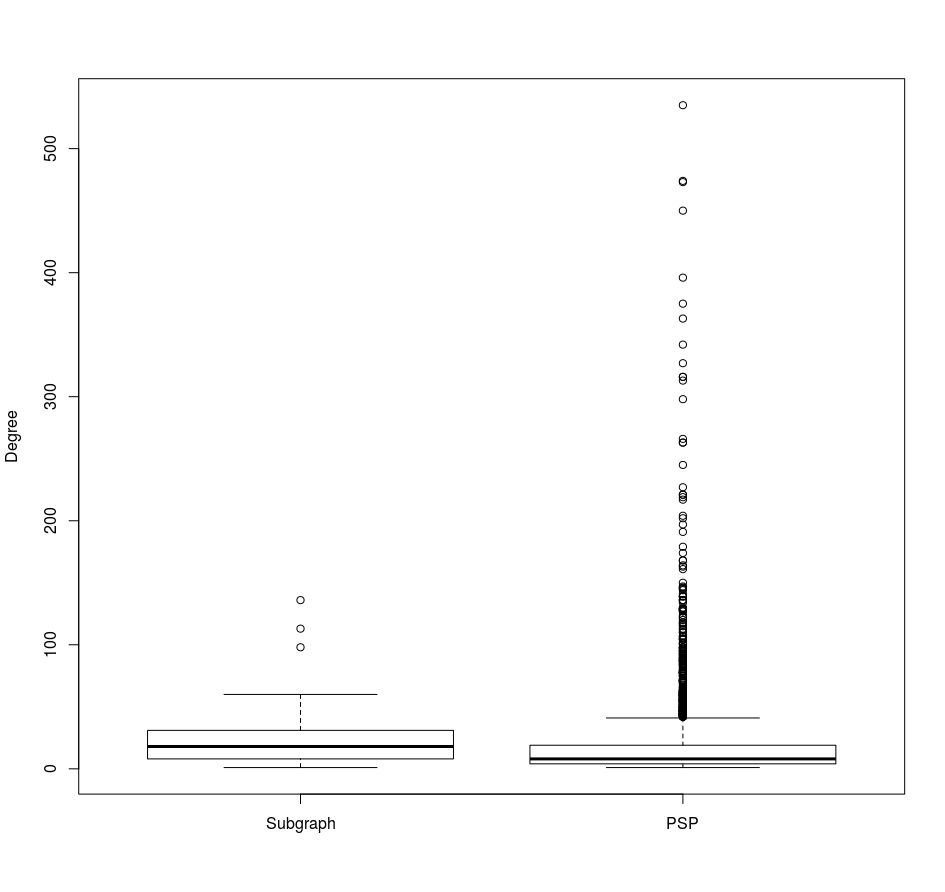
\includegraphics[width=\textwidth]{images/Rplot_boxplot_subgraph_and_PSP_degree.png}
    \caption{Degree distribution for induced subgraph of murine long term potentiation genes compared with PSP. The largest hub not has been removed from the subgraph.}
    \label{fig:Degree distribution for induced subgraph of murine long term potentiation genes compared with PSP. The largest hub not has been removed from the subgraph}
\end{figure}







\includegraphics[height=\baselineskip]{example-image}.
\begin{figure}
\includegraphics[height=3cm]{example-image-a}\includegraphics[width=5cm]{example-image-b}

\includegraphics[height=3cm]{example-image-a} \includegraphics[width=5cm]{example-image-b}
\caption{A figure}

\end{figure}




\chapter{Community detection}
\label{chap:community detection}
%\todo{Mpve spinglass to end}
\todo{Expand theory of spectral clustering}

 \todo{do citations for paper before moving}





\section{Introduction}
\todo{Rewrite this section as from paper eg DH}
\textcolor{red}{start of dh intro}
Intelligence, also known as general cognitive function,\cite{davies2015genetic} or simply as g,\cite{spearman1961general} describes the finding that across seemingly-disparate measures of cognitive ability, a single common factor explains around 40\% of the total cognitive test score variance in a group with a range of intellectual ability.  \cite{carroll1993human}  This single factor is the source of much of the predictive validity of cognitive tests; higher measured intelligence is predictive of higher-level educational and occupational outcomes, \cite{strenze2007intelligence}  as well as better health, and longevity .\cite{deary2012annrev} 

In twin and family studies genetic factors explain between 50-80\% of individual differences in intelligence. Using GREML-SC implemented in GCTA, \cite{yang2011gcta}  common single nucleotide polymorphisms (SNPs) have been found explain 20-30\% \cite{marioni2014common}  of differences in intelligence. When variants that are poorly tagged by genotyped SNPs are included using GREML-KIN, \cite{xia2016pedigree}  or GREML-MSC and imputed genotypes, around 50\% of the differences in intelligence can be explained using molecular genetic data. \cite{hill2018genomic} 

Consistent with the findings from other polygenic traits such as height, \cite{wood2014defining}  the number of variants associated with intelligence has increased as sample sizes have become larger. \cite{sniekers2017genome},\cite{hill2019combined}  However, the problem remains of how to transform information pertaining to phenotype-associated genetic loci into coherent biological explanations on how genetic differences result in phenotypic differences in intelligence. One such method that has been applied to intelligence is gene-set analysis (GSA). 

The logic of GSA is to examine a group of genes that are united by a common theme such as biologically-relevant mechanisms, \cite{hill2014human}  broadly constructed functional regions of the genome, \cite{hill2016molecular}  or being associated with a related phenotype. \cite{hill2016examining}  These gene sets are then examined against genes drawn from outside of the gene-set being tested using competitive gene set analysis (for a detailed discussion. \cite{de2016statistical}  Failure to compare the genes of interest against those from outside the set (i.e. to use self-contained gene set analysis) will result in an inflation of the alpha level. \cite{de2016statistical} 

GSA has indicated that the tissues of the brain and central nervous system are enriched for association with intelligence, \cite{hill2016molecular},\cite{johnson2016systems}  and has also been used to link transcription rate of genes expressed in the brain to genetic variation using genome-wide association study (GWAS) data sets on intelligence. \cite{hill2019combined}  Additionally, the NMDA- receptor signalling complex, a component involved in synaptic plasticity, has been shown to be associated for intelligence using competitive testing. \cite{hill2014human}  More recently, neurogenesis, the process by which new neurons are formed, as well as processes involved in the myelination of the central nervous system, have been implicated as biological mechanisms that bridge the gap between genotype and intelligence differences in humans. \cite{hill2019combined}  

\textcolor{red}{end of DH intro}
Effective synaptic function depends upon protein-protein interactions between over 2000 synaptic proteins (the synaptic proteome). Genetic variations in neuronal synaptic receptor components have been found to be enriched for differences in intelligence. \cite{hill2014human}  The complexes formed by these interactions have been described as ‘molecular machines’, and are a complex system with emergent structures and properties. \cite{grant2012synaptopathies}

Complex systems such as the synaptic proteome can be modelled as a network of nodes (vertices) joined by edges (links). In a network model of the synaptic proteome the nodes are genes that encode a synaptic protein and an edge shows that the protein products of two genes (nodes) interact. A network can be analysed at three levels: the network’s properties as a whole, the properties of individual nodes, or the presence of structures or organisation within the network.  \cite{newman2012communities}   
Many complex networks such as the internet, academic collaboration networks, and protein interaction networks share common properties at the level of the entire network. These properties include the small world phenomena or scale-free degree structures\cite{barabasi1999emergence},\cite{watts1998collective}  and provide evidence on how these networks form, how information passes through them and how resilient they are to disruption. \cite{rosvall2008maps},\cite{albert2000error},\cite{bianconi2001competition}  Recently the ‘small world property’ has been posited as a potential mechanism for an omni-genic model of genetic influence on complex traits. \cite{watts1998collective},\cite{boyle2017expanded} 


Communities  are the most well studied large-scale structure in networks. \cite{newman2012communities}  Communities are connected sub-graphs with dense interactions between community members and sparser connections to the rest of the graph. \cite{newman2012communities},\cite{fortunato2016community},\cite{girvan2002community} . They are not present in random graphs and are of interest because of their functional implications: in human and animal social networks they have been shown to correspond to real world grouping in the data, and these assignments can be made solely on the pattern of connectivity of the vertices. \cite{adamic2005political},\cite{zachary1977information}  An example of a community would be a group of friends in a social network; in the synaptic protein network, communities may represent functional modules and can therefore be used as gene sets for competitive GSA.  \cite{pocklington2006proteomes},\cite{mclean2016improved}  

Metabolic networks have been shown to contain hierarchical organisation and structure.\cite{ravasz2002hierarchical} Community detection methods when applied to synaptic protein networks and combined with over-representation GSA show differential enrichment of disease and Gene Ontology terms in particular communities. \cite{pocklington2006proteomes},\cite{mclean2016improved}  GWA studies results have been analysed with GSA using communities derived from protein interactions but the analysis was confined to genes achieving genome wide significance in 70 different disorders and the protein network used interactions derived from evidence other than direct interaction (such as co-expression) and was not tissue specific. \cite{ghiassian2015disease} 
Different tissues will contain different proteins and as a result the network will have different nodes and edges. Vertex (node) statistics such as degree will therefore be different and  community detection algorithms may give different results.

Many methods require the number of communities to be known (or guessed) in advance. Pocklington used the hierarchical divisive edge betweenness community detection method described by Girvan and Newman to perform community detection on an interaction graph of the NRC/MASC complex (248 edges, 105 nodes). \cite{pocklington2006proteomes},\cite{girvan2002community}  This has the advantage that the number of communities does not have to be determined in advance, the optimum level to stop the division is determined using an objective function, the modularity (Q), to determine the quality of the division of a network into communities. \cite{girvan2002community}  Modularity is a measure of the difference between the number of edges found between members of a community and the expected number of edges given the degree of the network. This is calculated using a random model of edge generation, the configuration model, where the degree of nodes is fixed and the edges assigned at random. \cite{fortunato2016community} 

Community detection can be posed as maximising the modularity over all possible divisions of the graph to obtain non-overlapping groupings of the nodes. \cite{newman2013spectral}  Modularity maximisation is computationally hard and a number of heuristics have been described to provide approximations to the optimal modularity. \cite{newman2013spectral} With increasing graph size many of these can become unstable, give rise to improbable community sizes, or become prohibitively computationally expensive. \cite{pocklington2006proteomes},41  
McLean et al \cite{mclean2016improved}  described a parallelized implementation of the edge betweenness algorithm used on the MASC complex   and found it to be prohibitively slow with large networks.  A powerful method of community detection that scales well with network size makes use of the spectral properties of the matrix representations of the network edges. \cite{newman2013spectral}  The network can be recurrently partitioned using the sign of the leading eigenvector of the modularity matrix. \cite{newman2013spectral}  McLean et al \cite{mclean2016improved}\todo{this just about repeats the previous two sentences} provide an implementation of this algorithm along with the random walk and edge betweenness algorithms optimised for computers with multiple cores. Examining the performance of these algorithms on a graph of the PSD they concluded the spectral clustering method with a fine-tuning step provided the best performance, measured by running time, community size and differential functional enrichment. 

Here we analyse a comprehensive and curated synaptic proteome network composed of the post synaptic density and its essential protein interactors. We combine this with the spectral clustering algorithm implemented by McLean shown to produce valid, and replicable communities in postsynaptic density complexes. \cite{mclean2016improved}  The community structures found in this network were then examined, using competitive GSA, to find if genetic variation in the genes encoding their proteins had an enriched association with a measure of cognitive ability, and one that has been used as a proxy for it: intelligence, and educational attainment. We examined whether any network node statistics are correlated with gene scores for intelligence or educational attainment.

This approach allows us to test three hypotheses aimed at contributing to understanding how genetic variation leads to individual differences in cognitive ability. Firstly, we test whether communities found in the post synaptic proteome graph are enriched for SNPs that have an effect on two measures of cognitive ability. Secondly, we test whether highly-connected hub nodes or other nodes that are influential in the network are associated with differences in human cognitive ability. Finally, we test the hypothesis that genetic variations in the protein complexes that surround the receptors, rather than just the receptors themselves, “interfere with the emergent functions of the protein set‚” 18  and play  a significant role in complex traits and diseases influenced by changes in synaptic function. 

This combined approach for analysis of neuropsychiatric GWA using synaptic structure can readily be extended to other disorders. 


\section{Methods}
To study the effect of synaptic network structure on the genetics of cognitive ability and educational attainment we have used a discovery and replication cohort design. To understand how the structure of the PSP might affect the genetic architecture of these complex phenotypes, we first tested if there was an association between measures of the influence of individual vertices (gene) in the graph (degree), and their significance in GWA studies. 
Next, we used GSA to test whether the genes encoding proteins forming community structures in the network were significantly associated with differences in intelligence or educational attainment. 

\subsection{Cohorts and studies}
\section{Cohorts and samples}

The population data used to test the association of centrality measures with population studies of educationbal attainment and intelligence were those described in sections~\ref{sec:cohorts from paper section} and \ref{sec:samples from paper section}



\subsection{Community detection – choice of algorithm.} 
To divide the network into its substructures wWe used a C++ implementation of spectral clustering with a fine tuning step in this paper as it previously provided the best balance of performance and informative functional enrichment on synaptic proteome networks. \cite{mclean2016improved}  The community structure is derived only from the pattern of network connections. i.e. no functional data is used to derived the substrucures.
Community detection was carried out using the CDS package onas described in \cite{mclean2016improved} using ECDF, the distributed computing facility provided by the University of Edinburgh. All other analysis was performed on an Intel® Core™ i7-7700K CPU @ 4.20GHz 8 core workstation running Ubuntu 16.04 LTS 64 bit.  
The modularity, a measure of the quality of the community prediction results, for the network partitioning was calculated in igraph library for R \cite{csardi2006igraph} . For all code see supplemental materials. 

\subsection{Network statistics}
To test the hypothesis that measures of gene importance in the network are correlated with cognitive ability and/or educational attainment, we calculated a range of standard network measures: betweenness centrality, degree, clustering coefficient, closeness centrality and eigenvector centrality using igraph for Python 3.6. \cite{csardi2006igraph}  We calculated the correlation between each of these vertex scores and the -log10 transform of the gene level p values derived from MAGMA for each study using Spearman’s rank correlation using the Scipy stats package for Python 3.6. 
\subsection{Study design Topology based GSA}
To test the hypothesis that there are network communities with an enriched association of genetic variations for intelligence and cognitive ability we carried out the following procedures.
Communities of genes within the PSP are identified using spectral clustering. Gene based statistics are then calculated for the discovery and replication cohorts. We then use GSA to analyse data from the discovery cohorts’ GWA analyses of intelligence and cognitive ability, to identify potential communities of interest. PSP communities of interest are then tested in independent replication cohorts with correction for multiple hypothesis testing. The study design is shown in figure 1.

\subsection{Gene Based Statistics}
We calculated gene based statistics for each study using MAGMA (v1.06) using the NCBI 37.3 assembly to identify gene boundaries. \cite{de2015magma}   No window was used around the gene boundaries. Linkage disequilibrium was corrected for using 1000 Genomes European data provided by the CTG lab with the MAGMA software version 1.6.\cite{de2015magma}  Commands used for gene based tests are found in the shell script in supplementary material. Data for the meta-analysis of intelligence performed by Sniekers  et al. was downloaded from the CTG website (see urls). \cite{sniekers2017genome}  The summary statistics for the EA2 study of educational attainment were obtained from the authors and excludes UKBiobank Phase II Education data (used as the discovery cohort) in addition to the data from 23 and me. \cite{okbay2016genome}  The summary statistics unsorted by sex were used for analysis. Summary statistics for Phase II of UKBiobank Education cohort and intelligence cohort were obtained from the co-authors directly from the CCACE.[ref]\todo{get ccace ref}

\subsubsection{PASCAL}
\label{sec:PASCAL community detection}
In order to determine if the choice of software for deriving a gene-based statistic influenced our results, we repeated our analyses using PASCAL instead of MAGMA, to provide both a gene level statistic and a competitive test of gene set enrichment. \cite{lamparter2016fast}  Pascal operates in a similar way to the popular VEGAS package but with a much shorter run time and the results are comparable. \cite{lamparter2016fast},\cite{liu2010versatile}  We judged it to be prudent to use an additional gene scoring method that uses a different scoring method as all subsequent analyses are dependent upon the gene score. 1000 Genomes European data was again used to account for linkage disequilibrium and no window was included around gene boundaries. The instructions supplied to the program are available in the supplementary material as a shell script. 

\subsection{Gene set selection}
We used the non-overlapping communities generated by the spectral community detection algorithm as gene sets stored in .gmt file format (each row a gene set). We represented each protein in the community by the Entrez ID representing the gene encoding that protein. 

We selected gene sets with more than 15 members. Divisive algorithms are known to often produce numerous small communities. Small gene sets can result in the signal being dominated by a single gene. We used the default lower limit gene size for the Gene Set Enrichment Analysis software, GSEA, as the lower limit (15). 54  

\subsection{Gene-set analysis}

We carried out gene set analysis using the inbuilt GSA function implemented in MAGMA and using the non -parametric competitive method implemented in GSEA. \cite{de2015magma},\cite{subramanian2005gene}  MAGMA provides a competitive gene set analysis using the regression weight of the association of the genes in the group with the phenotype. \cite{de2015magma}  We followed the advice of Wilmot and Mooney and used more than one enrichment method utilising GSEA to provide a non- parametric enrichment analysis. \cite{subramanian2005gene},\cite{mooney2015gene}  GSEA calculates the enrichment of a set of genes by calculating a running Kolmogorov-Smirnov score weighted by the p value of the gene in the gene level analysis. The -log10 transform of the gene level p values obtained using MAGMA were used as input for GSEA. Gene set enrichment analysis was carried out using the command line interface for the Java implementation of GSEA (GSEA - 3.0). The script to carry out the gene set analysis is included in the supplemental materials. 

We had no prior belief which, if any, communities would be associated with either phenotype. We therefore identified a set of genes (community) to be of interest if it attained nominally significant enrichment when tested using MAGMA GSA and GSEA. These gene sets were then used in the replication cohort GWA studies with correction of p values for multiple testing using the MAGMA permutation test and calculation of FDR q values in GSEA. Finally, the analysis pipeline was re-run using a different method of gene and pathway scoring to test whether the findings might be dependent on a particular package using PASCAL and its associated pathway analysis platform. \cite{lamparter2016fast}  

\subsection{Gene ontology enrichment}
To investigate the nature and function of significant community modules we used gene ontology enrichment analysis (see section~\ref{sec: gene ontology analysis}). \cite{mi2013large}  

 We tested for over representation of Gene Ontology terms in significant communities (sets) for each of the major Gene Ontology clades using Fishers exact test with corrections for multiple comparisons using the FDR method calculated using PANTER 13.1.\cite{mi2013large}We tested whether terms were over represented in these communities compared to their frequency both in the whole genome (using default  PANTHER settings) and compared with the  other 3457 genes in the PSP. \cite{mi2013large}  The ToppGene enrichment package was used to perform enrichment analysis of significant communities for murine and human phenotypes. \cite{chen2009toppgene}  

\subsection{Evolutionary Constraint}

The Exome Aggregation Consortium (ExAC - Broad Institute) contains DNA sequence data from the exomes of 60,706 individuals and provides metrics to identify genes subject to strong selection pressure against mutation. \cite{lek2016analysis}  We used data from version 1 (see URLs for source). This provides gene level measures of intolerance to deleterious mutations. The post synaptic density is known to be under evolutionary constraint with a low dN/dS (amino acid change/synonymous mutation change) in both murine and human PSD. \cite{ryan2009origin},\cite{bayes2012comparative},\cite{bayes2011characterization}  A bi-map was made between Ensembl transcript id in the ExAC data download and Entrez-id for the GRCh37 assembly using BioMart. \cite{smedley2015biomart}  We used the probability of the loss of function intolerance (pLI) to measure genetic constraint.

\section{Results}

\subsection{Synaptic Proteome Graph}

The largest connected component of the graph of the postsynaptic proteome (PSP) consisted of 3457 nodes and 30498 edges. The mean degree (the number of edges incident to each node) was 17.6, the median 8, minimum degree 1 and maximum degree 535. The degree distribution is consistent with a power law distribution. Further details on the graph are available in supplemental table 3. 

65 post synaptic graph communities (clusters) were detected using the spectral clustering algorithm with fine-tuning step; the modularity (Q) of the partition was 0.30 indicating a robust community architecture.  The communities ranged in size from 1 to 405 genes (mean 53.2, median 27, standard deviation 73). We excluded those communities with less than 15 members, removing 35 communities and 88 genes (2.5\% of the PSP). 35 communities with a total of 3369 genes remained with mean community size 96.1, median 72 and standard deviation 76.8 (See supplementary tables 4,5).   

\textbf{Gene level results}

Genome wide gene association analysis (GWGAS) was performed with MAGMA using the summary statistical data from the four cohorts. The results, including MAGMA output files, are available in the Supplemental Information.
Sniekers et al. found 47 genes associated with intelligence using MAGMA (Bonferroni threshold of P = $2.73 x 10^{-6}$). \cite{sniekers2017genome}  To confirm the validity of our gene level results we used summary data provided from this study and found 46 genes at  P$<2.74 x 10^{-6}$ genes using MAGMA v.1.06.  The pairwise correlation (Spearman’s $\rho$) of the negative log10 transformed gene p values reported in the supplementary material found in Sniekers et al and our results was $\rho$= 0.957. \cite{sniekers2017genome} 



\subsection{Gene set enrichment results}
In order to test the hypothesis that particular topological groups within the graph (communities) are enriched for genetic variants associated with differences in educational attainment or intelligence we carried out competitive Gene Set Analysis using the topological communities as gene sets. 
Four of 35 communities showed greater than nominally (p<0.05) significant enrichment using MAGMA GSA in the Education Discovery cohort (community: 5, P\textsubscript{MAGMA}=0.002, number of genes=106; community 53 n=405, community 22 n=42, P\textsubscript{MAGMA}=0.034; cluster 47 P\textsubscript{MAGMA}= 0.035 n=47). These communities other than 53 were among the 8 showing nominally significant enrichment using GSEA (2,5,11,20,22,24,33,47) and so communities 5, 22 and 47 (PGSEA= 0.004 ,0.014, 0.017) were taken forward to the replication cohorts. PGSEA for community 53 was 0.29. See table 2 and supplementary tables 2 and 3.
In the Intelligence Discovery cohort three four gene sets showed nominally significant enrichment using MAGMA GSA (cluster 10, p=0.008, n=146; cluster 5 p=0.014, n=106; cluster 22 p=0.046; cluster 53 p=0.049). However, only group community 5 showed at least nominally significant enrichment on GSEA and was analysed in the replication cohort. 
Group Community 5 was confirmed to have an enriched association with educational attainment in the replication cohort P\textsubscript{MAGMA}=0.01548, P\textsubscript{MAGMA} permutation= 0.043. Community Group 5 genes also were enriched in the Intelligence\textsubscript{Replication cohort} (p = 0.0084).

Gene set enrichment tests were also performed using the pathway function in PASCAL.\cite{lamparter2016fast} Community Group 5 showed significant enrichment in all four cohorts using PASCAL’s gene scoring and GSA analysis methods Education Discovery p=0.00007, Intelligence Discovery p=0.0001; Education Replication p=0.0003, Intelligence Replication p=0.0001; alpha Bonferroni 0.0015 (Supplemental table 8). 

\subsection{Gene ontology analysis}
We performed gene ontology enrichment analysis on community  5. Community 5 is significantly enriched for terms related to glutamate receptor activity and the heterotrimeric g protein complex, including the G protein coupled serotonin receptor. Community 5 has a significant proportion of these terms whether one compares against the rest of the genome or relative to other synaptic groups. 21 of the 27 genes annotated by the Gene Ontology Consortium as
glutamate receptor activity (GO:0008066 MF) are found in the PSP. Of these, 12 are found in group 5 (57.1\%). 
23 of the 37 genes encoding proteins annotated heterotrimeric g protein (GO:0005834) are found in the PSP. Of these, 16 are found in group 5 (69.5\% of PSP GO:0005834). 

The PANTHER over-representation test was carried out for each of the GO clades, Biological Process, Molecular Function, Cellular Component with the gene set compared with the 3457 PSP genes. The results are ordered by FDR and are presented in tables 9-11 in the supplemental material 

The biological process (BP) with the lowest FDR p value was G protein coupled receptor signalling activity, GO:0007186: FDR 2.16 x 10-8, fold enrichment 4.23. The second lowest was glutamate receptor signalling pathway GO 0007215: FDR 7.23 x 10-07, fold change 12.62.

Glutamate receptor activity GO:0008066 was also the most over represented molecular function term: FDR 7.58 x 10-07, fold change 16. The most enriched cellular component was GTPase complex GO:1905360: FDR 8.75 x 10-8, fold change 18.23. This was followed by heterotrimeric G-protein complex: FDR 1.75 x 10-7, fold change 18.23.

Enrichment analysis for ontology terms for Group 5 was also carried out with the entire genome  used to calculate the background frequency of terms (Panther default). Similar results with enrichment for g-protein associated receptors and glutamate receptors were found and shown in tables 12-14 in the supplemental material.

\subsection{Murine and Disease Phenotypes in Community 5}
The genes within group 5 have a strongly-enriched association with murine phenotypes related to synaptic transmission and electrophysiology. The top term is abnormal synaptic transmission (5.92 x 10-13 Bonferroni). We note that the 6th to 8th most enriched terms are phenotypes related to animal models of memory, learning and effective cognition (abnormal long term depression 6.41 x 10-7, abnormal synaptic depression 1.31 x 10-6 and abnormal long term potentiation 1.4 x 10-6, P values with Bonferroni correction using ToppGene \cite{chen2009toppgene} ). See table 15 in the supplemental material.

Group 5 has an enriched association with genes that have been reported to be implicated in the aetiology of common neuropsychiatric disorders. The ten most significant terms using ToppGene \cite{chen2009toppgene}  include Schizophrenia (p = 5 x 10-08), Major Depressive Disorder (p = 6.06 x 10-5),  Bipolar Disorder (p=1.74 x 10-3), Substance induced Psychosis  (3.39 x 10-3) and Unipolar depression (p=9.14 x 10-03). See table 16in the supplemental material.

\subsection{Subgroup analysis}
Two large components can be identified in community 5 using gene ontology: heterotrimeric g proteins (of which G-protein coupled serotonin receptor complex is a subset) and glutamate receptors. These are strongly associated with human disease phenotypes and murine models of cognitive ability.

With a community gene set discovered using only network topology, Gene Ontology can be used to provide a finer dissection of community properties (for example all the members of a community and all those that do or do not belong to a GO annotation that is predominant in the group).

We find that the genetic variations in G protein receptors and glutamate receptors do not have an enriched association with educational attainment or human cognitive ability as one might expect based on animal phenotypes; rather, the remaining genes in group 5 after these have been removed have increased enrichment for educational attainment or intelligence, except in the CTG cohort (see table 17 supplemental material), but have a weaker association with human disease phenotypes and murine models of cognition. 

Cluster 5 contains 112 genes. This cluster is enriched for genetic variants associated with intelligence and cognitive ability in all four cohorts (Intelligence Discovery p=0.014, Education Discovery p=0.002, Intelligence Replication p= 0.008, Education Replication p=0.015). There are 31 genes related to the heterotrimeric g protein complex, glutamate receptor activity or other G proteins (GO:0008066 and GO:0005834, 3 x GNB). The 81 genes left in the cluster after these are removed show more significant enrichment in all cohorts except IntelligenceReplication  (Intelligence Discovery 0.005 2.8x, Education Discovery p=0.0002 increase 10x, Intelligence Replication 0.013 (0.61 x), Education Replication (p=0.002, 7.5 x).
 
\subsection{Genetic Constraint}
We used the probability of loss of function intolerance (pLI) measure in the ExAC database as a measure of genetic constraint. \cite{lek2016analysis} 

The median pLI 54.1\% and the mean pLI was 1.85\% for all genes that appear at least once in the four cohorts (n= 17928). The glutamate receptor associated genes in community 5 are under much greater constraint (Mean pLI 86.2\%, median pLI 99.5\%) than the rest of the PSP (mean pLI 50.3\%, median pLI 50.4\%) or community 5 as a whole (mean 61.2\%, median 82.8\%).
(supplemental table 18). 
There was a small, significant positive correlation between -log10 transformed P gene association statistics for the cohorts and -log10 pLI (rho 0.12, p=3.5 x 10-11). The results are shown in supplementary table 19.

\section{Discussion}
Our results suggest that genetic variation in the genes encoding a group of proteins forming a tightly interconnected subnetwork in the post synaptic proteome have an enriched association with differences in educational attainment and intelligence. This group contains the majority of the genes encoding glutamate receptors and heterotrimeric G protein in the post synaptic proteome. These genes are commonly found in animal models of learning and memory and would intuitively appear to have a role in human learning and intelligence. The enrichment signal is, however, found in the neighbours of these proteins.

This paper is to our knowledge the first to use GSA in association with community detection and make use of the complete data present in GWAS summary results. Ghissian recently used the Louvain algorithm in association with the STRING protein database but did not use a tissue specific network or a competitive test of GSA and the GWA data was limited to significant genes on GWA catalog. \cite{ghiassian2015disease} 

In particular we have used an interaction network specific to a cellular component implicated in the trait. Goh found that genes that were specific to tissues were more likely to be associated with diseases than others in the connectome \cite{goh2007human}  and this seems to extend to complex traits at least in the form of intelligence and educational attainment. The review by Mooney and Wilmot of gene set analysis discusses sub communities detected in protein interaction networks as possible gene sets \cite{mooney2015gene}  and gives an example of a modularity maximisation method and an annotation mining tool that incorporates module detection; however, the first does not use genetic data and the second implements an over-representation test. does not use the full amount of data from GWA and the web address given in the paper is broken. 64  This technique could be extended to other disorders or complex traits that may be mediated by synaptic function. The synapse may behave differently from other tissues in these forms of analyses, as we know it forms modular units from its proteins that are associated with function \cite{grant2012synaptopathies} , and our finding might not generalise to proteomes in non-synaptic tissue or metabolic pathways. 

We found no association between gene level GWA p values for educational attainment or intelligence and measures of vertex importance such as degree. It may be that nodes of high degree result in a severe phenotype and are not represented in population studies of complex traits. We would hypothesise that these core nodes are necessary for basic functions, and this is supported by the finding that the nodes that have a high level of importance on each of these metrics are associated with an increased measure of evolutionary constraint. 

 	Our findings extend those of Goh to complex traits and show that genes whose variants are significantly associated with differences in cognitive ability or educational attainment are not disproportionately those of high degree.\cite{goh2007human} 
 The terms discovered using disease enrichment are heterogenous and come from animal models and databases such as OMIM and var. However, their use as indicators of an enriched association with a disease is common in the previous literature on network approaches to human disease. It is therefore desirable to have an approach incorporating all the information in the summary data of GWA study in the analysis of the association of network statistics or structures with disorders or complex traits.
 
The group is composed of glutamate receptors and G protein complexes intimately related to the plasma membrane corresponding to receptor complexes and their supporting proteins. Glutamate mediated neurotransmission is required for initiation of long term potentiation, and blocking glutamate receptors in the hippocampus of mice causes failure of memory encoding. 65,66  More recently, differential expression of glutamate receptors have recently been shown to be associated with differences in problem solving in two species of wild finch. \cite{audet2018divergence}  

The glutamate receptors and heterotrimeric G proteins are not however the source of the enrichment signal and the potential connection between the GWA findings and these receptors is made possible by this analysis of communities within the graph structure.

A small world model of genetic influence networks has been argued to support an omni-genic model of traits. \cite{boyle2017expanded}  However the structure of the synaptic graph may affect the genetic architecture of complex traits, even in a undirected network with unweighted edges and a small world structure, the rate of flow of information between genes depends on network structure.

There are limitations to the current study. The set of genes found in proteomic studies of the pre and postsynaptic areas continues to increase although the \cite{heil2018systems} increase has reached a plateau. 41  If the network changes then the community allocations will change and a different network may lead to different community allocations. We have tried to limit this effect by choosing the method with the lowest proportion of ambiguously clustered pairs (PAC).

The community allocations in addition are not a globally optimal allocation with regard to the modularity, and alternative partitions with similar modularity exist. The Spin glass model was an attractive alternative clustering method but has a number of tuneable parameters making designing a study which would properly account for multiple testing challenging.\todo{change 47 to spinglass ref}47 

The clustering also does not take consideration that nodes may belong to more than one component or cluster. Probabilistic methods exist to determine the most likely community membership if vertices can belong to more than one community73 but the loss of non-overlapping gene sets may result in a great increase in the number of sets. We have also not taken into account a model where some genes are assigned to communities while others remain unassigned.

The question of whether communities represent some ground truth entity also exists \cite{peel2017ground}  and we have not used any data other than the distribution of edges in community detection but it is possible to introduce these.  \cite{newman2016structure} 


 

\subsection{Extra results:Remaining proteins after subgroup}
Remaining enrich for neurogenesis but the number of neurogenesis genes are low. Hill showed enrichement for neurogenesis genes but tested over 1000. Signal we have is from approx 7 and we also see enrichment in other areas close to glutamate synapses
check path\_to\_code2

\url{source('~/RProjects/go_analysis/R_src/GO_entity/load_neurogenesis.R')}

\url{source('~/RProjects/utils/src/generic_compile_gsa_neurogen.R')} MAC
This shows that there is not consistent enrichment for neurogenesis in group 5 22 genes associated with it 
\begin{table}[]
    \centering
    \begin{tabular}{lllllll}
        SET& NGENES&    BETA &BETA\_STD  &  SE      &   P  & P\_C\\
        \hline
  5  &   22&  0.2410&  0.00837& 0.237& 0.1537900& 0.0015956\\   
         & 
    \end{tabular}
    \caption{Intelligence neurogenesis}
    \label{tab:Intelligence neurogenesis}
\end{table}

\begin{table}[]
    \centering
    \begin{tabular}{lllllll}
        SET& NGENES&    BETA &BETA\_STD  &  SE      &   P  & P\_C\\
        \hline
  5   &  22&  0.7930&  0.027500& 0.242& 0.00052570 &0.1371100\\

 \end{tabular}
    \caption{Education neurogenesis}
    \label{tab:Education neurogenesis}
\end{table}

Group 36 enriches in all but EA3 but has only 4 neurogenesis genes \todo{What is enrichment in full gsa}


\section{Louvain}


\subsection{Introduction}
The Louvain method named after the university of the authors of the original paper is a hierarchical clustering method using modularity maximisation as the objective function. It functions very well at scale in dividing networks up into communities.\cite{blondel2008fast}

The algorithm works by first assigning nodes into communities. Then those communities are in turn combined into communities composed of communities. The process stops when maximal modularity is achieved. 

\subsection{Methods}

Louvain clustering was carried out using igraph Version 1.2.4.2 using the \texttt{cluster\_louvain} command. The Louvain implementation requires no parameters to be supplied other than an optional weights argument for weighted networks and this simplifies study design as described earlier. 

The igraph implementation returns communities discovered at the level of hierarchy that maximises the modularity.

The communities objects returned by the \texttt{cluster\_louvain} method were converted into a gmt file using a custom R script.\todo{source}

Gene set analysis of the educational ability and intelligence GWA were carried out using MAGMA as described above \todo{add cross ref}. 



\subsection{Results}
Louvain clustering discovers 14 communities in the PSP. The modularity of the resulting division is 0.339.

Group 7 shows enrichment in the intelligence discovery (p=0.0012) and replication cohorts (p=0.0026). Group 7 is composed of 154 genes but the number shown in the tables of results may be less than this if a gene was not assigned any SNPs using MAGMA. Using a discovery and replication cohort alpha is 0.0125, but the enrichment is greater than considering all of the groups alpha 0.00357 (0.05/14). See table~\ref{tab:Louvain clustering intelligence}

Group 7 is enriched in the discovery cohort for education but not the replication cohort (p=0.0146 and replication p=0.4750). See table~\ref{tab:Louvain clustering education}.

Using the largest cohorts available for intelligence we confirm group 7 is enriched (Savage) p=0.0002. Two other groups survive multuple testing at alpha corrected for all groups see table~\ref{tab:Louvain clustering Savage intelligence phase 2 cohorts}. 

Using the largest cohorts available for education we find enrichment of group 7 (p=0.0017) and the group 8 found in Savage (p=0.0003) see table~\ref{tab:Louvain clustering EA3 Education cohorts}
% latex table generated in R 3.6.1 by xtable 1.8-4 package
% Sat Mar 28 15:46:38 2020

Group 7 is enriched for Molecular function glutamate receptor activity GO:0008066 	glutamate receptor activity 		 	Bonferroni (against genome) $3.478 \times 10^{-32}$ 	Number in group 26  In annotation	84. 
Group 8 is large. The second most enriched Biological process is GO:0048666 	neuron development 		Bonferroni	$1.180 \times 10^{-52}$ 	Number in group 150 	Number in annotation 1298.

Code on mac \url{source('~/RProjects/utils/src/generic_compile_gsa_lourvain_new.R')}
\todo{Overlap of group 7 with group 5}
\begin{table}[ht]
\centering
\begin{tabular}{rlrrrrrr}
  \hline
 & SET & NGENES & BETA & BETA\_STD & SE & Intelligence Discovery & Intelligence Replication \\ 
  \hline
2 & 2::: & 334 & 0.09 & 0.01 & 0.05 & 0.0407 & 0.1916 \\ 
  3 & 3::: & 510 & 0.10 & 0.02 & 0.04 & 0.0075 & 0.1006 \\ 
  7 & 7::: & 144 & 0.26 & 0.02 & 0.08 & 0.0012 & 0.0026 \\ 
  12 & 12::: & 21 & 0.63 & 0.02 & 0.21 & 0.0014 & 0.1628 \\ 
   \hline
\end{tabular}
\caption{Louvain clustering PSP Intelligence cohorts}
\label{tab:Louvain clustering intelligence}
\end{table}

% ed

% latex table generated in R 3.6.1 by xtable 1.8-4 package
% Sat Mar 28 15:49:04 2020
\begin{table}[ht]
\centering
\begin{tabular}{rlrrrrrr}
  \hline
 & SET & NGENES & BETA & BETA\_STD & SE & P & P\_EA2 \\ 
  \hline
2 & 2::: & 334 & 0.13 & 0.02 & 0.05 & 0.0071 & 0.0568 \\ 
  5 & 5::: & 112 & 0.23 & 0.02 & 0.09 & 0.0063 & 0.3478 \\ 
  7 & 7::: & 144 & 0.19 & 0.02 & 0.09 & 0.0146 & 0.4750 \\ 
   \hline
\end{tabular}
\caption{Louvain clustering PSP Education cohorts}
\label{tab:Louvain clustering education}
\end{table}

% latex table generated in R 3.6.1 by xtable 1.8-4 package
% Sat Mar 28 15:51:04 2020 Sav2
\begin{table}[ht]
\centering
\begin{tabular}{rlrrrrr}
  \hline
 & SET & NGENES & BETA & BETA\_STD & SE & P \\ 
  \hline
2 & 2::: & 345 & 0.11 & 0.02 & 0.0550 & 0.0208 \\ 
  3 & 3::: & 527 & 0.11 & 0.02 & 0.0431 & 0.0055 \\ 
  7 & 7::: & 153 & 0.32 & 0.03 & 0.0899 & 0.0002 \\ 
  8 & 8::: & 537 & 0.14 & 0.02 & 0.0475 & 0.0018 \\ 
   \hline
\end{tabular}
\caption{Louvain clustering PSP Savage Intelligence phase2 cohorts}
\label{tab:Louvain clustering Savage intelligence phase 2 cohorts}
\end{table}


% latex table generated in R 3.6.1 by xtable 1.8-4 package
% Sat Mar 28 15:52:19 2020
\begin{table}[ht]
\centering
\begin{tabular}{rlrrrrr}
  \hline
 & SET & NGENES & BETA & BETA\_STD & SE & P \\ 
  \hline
1 & 1::: & 196 & 0.11 & 0.01 & 0.0897 & 0.1185 \\ 
  2 & 2::: & 334 & 0.06 & 0.01 & 0.0660 & 0.2021 \\ 
  3 & 3::: & 510 & 0.08 & 0.01 & 0.0521 & 0.0740 \\ 
  4 & 4::: & 245 & 0.10 & 0.01 & 0.0792 & 0.0943 \\ 
  5 & 5::: & 111 & 0.09 & 0.01 & 0.1110 & 0.2132 \\ 
  6 & 6::: & 159 & 0.01 & 0.00 & 0.0958 & 0.4421 \\ 
  7 & 7::: & 144 & 0.32 & 0.03 & 0.1080 & 0.0017 \\ 
  8 & 8::: & 519 & 0.19 & 0.03 & 0.0558 & 0.0003 \\ 
  9 & 9::: & 425 & 0.04 & 0.01 & 0.0640 & 0.2426 \\ 
  10 & 10::: & 57 & 0.03 & 0.00 & 0.1570 & 0.4303 \\ 
  11 & 11::: & 331 & 0.08 & 0.01 & 0.0679 & 0.1087 \\ 
  12 & 12::: & 21 & -0.11 & -0.00 & 0.2620 & 0.6587 \\ 
  13 & 13::: & 80 & -0.12 & -0.01 & 0.1330 & 0.8143 \\ 
  14 & 14::: & 166 & 0.09 & 0.01 & 0.0989 & 0.1692 \\ 
   \hline
\end{tabular}
\caption{Louvain clustering PSP EA3 Education cohorts}
\label{tab:Louvain clustering EA3 Education cohorts}
\end{table}



\section{Spinglass}

There are a number of tunable parameters for the implementation of the spinglass algorithm in igraph for R specifically
args for spinglass
\begin{itemize}
    \item{weights not applicable - edge weights}
    \item vertex - community for specific vertex ignore
    \item spins default 25 - upper limit for number of communities
    \item parupdate false not required
    \item start.temp default 1
    \item stop.temp 0.1
    \item cool.fact for simulated annealing
    \item update simple or random or config we may need config
    \item gamma = balance between present and non present edges in a community present and non present edges default 1.0 makes existing and non existing links equally important, smaller make existing links, greater missing links more important
\end{itemize}









\todo{Check enrichment}


\subsection{Theory behind spinglass}
\todo{remember local clustering}
\todo{remember reasons for looking for communities around or less than 100 Leskovec paper on peak conductance}

\subsection{Implementation}
Spin glass clustering was carried out using the igraph package in R using a script to automatically generate values for gamma and spins and to conver the communities object into a graph markup language(GML) file. 5 gamma values were used gamma = $0.1,0.5,1,2,5$ and 9 spin values spins = $2,10,20,30,40,50,60,80,100$ 
Running 45 grid search the clustering with spinglass takes about 56.6 seconds which accumulates if one has a large number of clusters to make therefore Grid search generation run on staff.compute R 3.5 DICE.
Gamma of 0.1 and 0.5 only returned valid spins of 2 and 2,10 respectively. 
\subsection{Study design}
Given the number of tunable parameters in the spinglass model it is difficult to make a study design similar to that we used with the spectral clustering as the number of communities will lead to a prohibitively small alpha level. The possibility of finding individual datasets for each set of communities at each parameter setting is not practicable as even varying only gamma and spins we have the cartesian product of the number of parameter settings numbers of groups of sets.

The number of spins controls the maximum number of groups found in the clustering. The value of gamma controls the importance of there being edges present within the commmunity modules.

We would however prefer not to abandon spin glass entirely. McLean (personal commmunication) found it gave good community enrichment at certain values (higher values) of gamma. However we are also aware both from theory and our earlier experiment that pure modules in the ontology sense may not be what we want. We may want a dominant ontology group and their neighbouring proteins that form a module as this may map more reliably onto population data. Also although it is attractive the ontology group is in no sense a ground truth it is still 'Menschenwerk' (Kronecker).

One option is to adopt a strategy from machine learning. We will define the discovery intelligence and education as the training set and find the groups of sets that have a set with an arbitrarily low p value and of a satisfactory size. We will then combine these into a group of sets and test these on the replication cohorts. The design is not so robust as the previous one but at least allows us to see what insights we might gain from the spin glass clustering. We are not randomly sampling from the synaptic proteome there is still the constraint that we require that the sets form modules (in terms of their edge in-out distribution) and that the modules are connected subgraphs of the network. The arbitrary element (or the most arbitrary element) of this design is the choice of alpha. We want to chose alpha such that the number of sets to test in the replication does not lead to excessive type II error. The lower we choose alpha for the first set the more likely the p value of the second set is to be low. We can also try using the nominal alpha level of 0.5 and see what we get. 

\subsubsection{Spinglass results}
We get significant enrichment for spin 2 gamma 5 for education and intelligence both sets. This is because we are splitting the PSD in two. The larger approx 2082 number of genes is the one that enriches.

For spins 10 gamma 5 we get 10 groups the 417 number group enriches strongly in discovery and replication but not for education and it is a big group.



\todo{Modularity}
\subsection{Modularity}

Although the modularity of a partition of random graph tends towards 0 we can calculate the modularity of a randomly wired graph with the pre-existing group allocations \footnote{\url{source('~/RProjects/centrality/R/bootstrap_ci_modularity.R')}}

We can also calculate the modularity for clustering a random graph. Louvain 1000 iterations.
  Min. 1st Qu.  Median    Mean 3rd Qu.    Max. 
 0.1468  0.1577  0.1602  0.1601  0.1627  0.1706 
 
 distribution of results near normal. 	Shapiro-Wilk normality test

data:  results
W = 0.99726, p-value = 0.0877

Mean centred = same 0.0877

The degree distribution is part of the results. 

The values are lower using random degree sequences but not all are valid here is an example we would have to do try except better in python \footnote{\url{source('~/RProjects/centrality/R/bootstrap_ci_modularity_louvain_cluster_resampling.R')}}

   Min. 1st Qu.  Median    Mean 3rd Qu.    Max. 
 0.1427  0.1504  0.1529  0.1527  0.1552  0.1626 
 
 Barabsi.game with n=3457 and gamma = 2.7
 \footnote{\url{source('~/RProjects/centrality/R/bootstrap_ci_modularity_louvain_cluster_barabasi.R')}}
 

It is significantly enriched for glutamate receptor activity (37 of 84) and axon guidance and for ASD, schizophrenia and seizures \todo{overlap with group 5}. 

It also enriches significantly in EA3 group 5(Spinglass) $P=0.0010319$ but so does group 9 at p=$0.0014555$

src \url{source('~/RProjects/gridsearch_gamma/R/check_results/check_results.R')}

Enriches strongly in savage $0.0049343$ but less so in davies (approx 0.02 but group 4 very strongly in davies)

 \section{Community detection thresholds}
There are limits to the detection of communities specifically in the difference between the probability of edges and the probability of in group edges.
 
 \section{Enrichment of the presynaptic proteome}
 
 Surprisingly all of the education phenotypes enrich for genes in the presynaptic proteome and this is not true of intelligence except weakly for UKBB Intelligence Discovery. The reasons for this are unclear. See figure \ref{Table:Enrichment of intelligence phenotypes presynaptic proteome} and \ref{Table:Enrichment of education phenotypes presynaptic proteome}
 
 % latex table generated in R 3.6.1 by xtable 1.8-4 package
% Thu Jan 16 16:01:27 2020
\begin{table}[ht]
\centering
\begin{tabular}{rlrrrrr}
  \hline
 & SET & NGENES & BETA & BETA\_STD & SE & P \\ 
  \hline
1 & Education Replication\_presynaptic\_all & 1449 & 0.06 & 0.02 & 0.02 & 0.00 \\ 
  2 & Education Discovery\_presynaptic\_all & 1461 & 0.07 & 0.02 & 0.03 & 0.00 \\ 
  3 & EA3\_presynaptic\_all & 1460 & 0.10 & 0.03 & 0.03 & 0.00 \\ 
   \hline
\end{tabular}
\caption{Enrichment of education phenotypes presynaptic proteome} 
\label{Table:Enrichment of intelligence phenotypes presynaptic proteome}
% latex table generated in R 3.6.1 by xtable 1.8-4 package
% Thu Jan 16 16:01:27 2020
\end{table}

\begin{table}
\centering
\begin{tabular}{rlrrrrr}
  \hline
 & SET & NGENES & BETA & BETA\_STD & SE & P \\ 
  \hline
1 & Education Replication\_presynaptic\_all & 1449 & 0.06 & 0.02 & 0.02 & 0.0048 \\ 
  2 & Education Discovery\_presynaptic\_all & 1461 & 0.07 & 0.02 & 0.03 & 0.0032 \\ 
  3 & EA3\_presynaptic\_all & 1460 & 0.10 & 0.03 & 0.03 & 0.0020 \\ 
   \hline
\end{tabular}
\caption{Enrichment of education phenotypes presynaptic proteome} 
\label{Table:Enrichment of education phenotypes presynaptic proteome}
\end{table}


% latex table generated in R 3.6.1 by xtable 1.8-4 package
% Thu Jan 16 16:01:27 2020
\begin{table}[ht]
\centering
\begin{tabular}{rlrrrrr}
  \hline
 & SET & NGENES & BETA & BETA\_STD & SE & P \\ 
  \hline
1 & Intelligence Discovery\_presynaptic\_all & 1461 & 0.05 & 0.01 & 0.03 & 0.04 \\ 
  2 & Intelligence Replication\_presynaptic\_all & 1466 & 0.02 & 0.00 & 0.02 & 0.23 \\ 
  3 & Savage\_presynaptic\_all & 1498 & 0.04 & 0.01 & 0.03 & 0.10 \\ 
  4 & Davies\_presynaptic\_all & 1460 & 0.05 & 0.01 & 0.03 & 0.04 \\ 
   \hline
\end{tabular}
\caption{Enrichment of intelligence phenotypes presynaptic proteome} 
\label{Table:Enrichment of intelligence phenotypes presynaptic proteome}
\end{table}

% latex table generated in R 3.6.1 by xtable 1.8-4 package
% Thu Jan 16 16:01:27 2020
\begin{table}[ht]
\centering
\begin{tabular}{rlrrrrr}
  \hline
 & SET & NGENES & BETA & BETA\_STD & SE & P \\ 
  \hline 

1 & Intelligence Discovery\_presynaptic\_all & 1461 & 0.05 & 0.01 & 0.03 & 0.04 \\ 
  2 & Intelligence Replication\_presynaptic\_all & 1466 & 0.02 & 0.00 & 0.02 & 0.23 \\ 
  3 & Savage\_presynaptic\_all & 1498 & 0.04 & 0.01 & 0.03 & 0.10 \\ 
  4 & Davies\_presynaptic\_all & 1460 & 0.05 & 0.01 & 0.03 & 0.04 \\ 
   \hline
\end{tabular}
\caption{Enrichment of intelligence phenotypes presynaptic proteome \url{'~/RProjects/paper_xls_output/R/make_pLI_correlation}...., line 507} 
\label{Table:Enrichment of intelligence phenotypes presynaptic proteome}
\end{table}

Those of low betweeness are a slightly smaller group but enrich more in ea2 and ukbbed. Todo correlation of graph degree etc and study in presynaptic. \url{source('~/RProjects/graph_distances/R/collate_presynaptic_edubet.R')}
 

The most enriched genes in toppgene are labelled as post synaptic including BSN, SHANK3 and CAMKV. There is overlap between presynaptic and PSP (\todo{how much overlap}) A large number of the highest scoring presynaptic genes are listed as post synaptic in toppgene. \todo{MAGMA GSA for toppgene presynaptic genes}

\todo{what are setgenesout for all post synaptic or murine}
%\chapter{removed from paper}

\section{title and authors}
Spectral clustering reveals a role for the glutamatergic receptor complex in human cognitive abilities

Robertson, G, Hill W D, McLean C, Sorokina O, [Heil, Emilia?],[other CCACE] [EA2
people who got the data without UKBB],Simpson IT, Deary IJ, Armstrong JD



\section{abstract}
Abstract

Abstract: 150-250 words 
142 words
20.09 187 words
Introduction: 1,500 words
2039 at present
1634 at present 11.09
1641 24.09
Article: 3,500 words, excluding abstract and references.
5846 words at present
4730 at present 11.09
4572 words.


Max of 5 Figures and tables –
 2 figures and 2 or 3 tables depending on version chosen
19 supplemental tables
Max of 75 References – 70 ref just now, 69 just now

Abstract (187 words)
The proteins that interact in the region of the neuron’s post synaptic density, the post synaptic proteome (PSP), have a modular structure and their function is profoundly affected by the pattern of their interactions.
Previous studies have shown an enriched association between genetic variations in synaptic genes and individual differences in measured intelligence. We describe, using community detection methods, meso-scale structures in the PSP we can divide the PSP into substructures based on molecular interactions. Using competitive gene set analysis in MAGMA, we investigate whether any of these substructures (communities) have an enriched association with intelligence or the related phenotype of educational attainment. We use genetic data from UK Biobank (n=120 934 intelligence, n=273 274 educational attainment) to show that a community closely associated with glutamate receptors has an enriched association with intelligence and educational attainment (p=0.002 Education, p=0.014 Intelligence). We replicate these findings using similar but non-overlapping cohorts (Education n=217 569, p=0.0084; Intelligence n=78 308, p=0.015, alpha Bonferroni 0.045). We find that the source of the enrichment signal is not the glutamate receptors themselves but their interaction neighbours, a finding which would not be apparent using standard manually curated approaches gene-sets (e.g. GO, pathways) to generating gene sets for (GSA).

  


\section{From centrality}
\subsection{Presynaptic proteome}



\section{Disease modules}
\section{GSA}
\subsection{rnk files}
Link behind comment \url{http://software.broadinstitute.org/cancer/software/gsea/wiki/index.php/Data_formats#RNK:_Ranked_list_file_format_.28.2A.rnk.29}
\clearpage{}




%\chapter{Core periphery structure} 

Rombach Core periphery revisited – generates continues value coreness for each node

Borgatti and Everett

Hubs are commonly found in empirical networks and pose a problem for community detection as they usually have strong ties to many communities. Identifying core–periphery structures can help circumvent this problem by categorizing hubs as part of the network's core (Rombach et al., 2014, p. 160).  (from Wikipedia)

ref Rombach, M. P., Porter, M. A., Fowler, J. H., \& Mucha, P. J. (2014). Core–periphery structure in Networks. SIAM J. Appl. Math., 74(1), 167–190.

Chung and Lu power law random graph with beta element [2,3] contains core

from Rombach
Core (hub) nodes can have strong ties to different communities

Communities as tiles that overlap to produce network core Yang and Leskovec

Original paper

1 Intuitively different concepts can bemathematically similar eg global core periphery with local community structure, globaql community structure with local core peripehry and network with multiple core periphery pairs

II search for various cores with a sizer and shape parameter (rather than a global optimum like odularity)

Core periphery strcutre is often correlated with measures sucha s degree centrality, eigenvector centrality, betweenness centrality and page rank although these are intuitively different concepts

also different from rich clubs (see Zhang and Newman)

Borgatti and Everett have a multi core model too (in bib ccohesive subsets)

Kojaku and Masuda also have algorithm for multiple cores (GR and cdode for a significance test for networks)

Zhang and Newman use block model which has also been used by Peixoto to study core periphery (including nested)

Spectral partitioning for core periphery
Cucuringu adjacency as low rank perturbation matrix
Barucca spectral regularities for core periphery

Some spectral methods rely on edge density (bit like community structure)
others transport where core nodes are likeloy to be on shortest paths
Curucuringu again and Lee, Cucuringu and Porter use a transport based coreness

k core fast but like requiring a community to be a network clique



Other cp

Luo 2009 Core periphery in PPI

Other stuff

Benchmarks


TTD
Coreness in igraph seems to pick ou (surprisingly core nodes – lethality etc inc housekeeping) and peripheral (more specifically synaptic associated with transmission).
Add to centrality measures
Try enrichment gmt with removal of k core
Try induced subgraph with k core removed



\section{Introduction}
\subsection{The leading eigenvector and coreness}
The principle eigenvector is all negative in the graph it is also all negative in core periphery structures
There is a linera relationship with both betweeness centrality but more particularly degree

So I have read about this today and it is a consequence of Perron-Frobenius theorem
If you select the most negative values you pick out a lot of ribosomal components and get very strong enrichment for GO categories.
Disease ontologies are neoplastic and these genes are essential

Low values gets epilepsies, lots of specific neuronal transmitter stuff

\todo{do with background PSP}
If you take the row eig eig\$vector[1, ] you get the sign of all the eigenvectors for that gene. It is symmetrical too about the midline (?because matrix symmetrical and of equal values)

Lowest quartile of second eigenvector - lots of actin and cytoskeletal, schizo and adhd

highest quartile of second eigenvector - RNA binding, ribosome, lethality, non homogenous diseases


Lowest 230 ish of second eigenvetor - 80 actin binding and 54 cadherin

5th lowest centile 2nd eigenvector - 72 actin binding 45 cadherin

Pseudo spokes have low principle eigenvectors

Pseudo hubs have lower leading eigenvector than overall but less than pseudospokes

Ps vs ph
W = 1602, p-value = 0.03092
Wilcoxon

wilcox.test(eig\_filter\_ph,vec)

        Wilcoxon rank sum test with continuity correction

data:  eig\_filter\_ph and vec
W = 19194, p-value = 5.552e-06
alternative hypothesis: true location shift is not equal to 0

> wilcox.test(eig\_filter,vec)

        Wilcoxon rank sum test with continuity correction

data:  eig\_filter and vec
W = 42907, p-value < 2.2e-16
alternative hypothesis: true location shift is not equal to 0
\section{SNAP}

\subsection{Previous}
The file \url{/home/grant/Dropbox/PhD/Core\_Periphery/SBM\_snap.odt}

Shows that the maximum likelihood is at 5 groups in SNAP. I have not yet located the gml. From memory these are overlapping. I think this might have been a graph from making a five group planted SBM.

The snap single core single periphery gmt file is at MAC \url{ gene\_set/ctg\_PSP\_3457\_SNAP\_core\_and\_complement.gmt.sets.out}

There is a sbm\_2\_group in utils R on laptop which I think is when I made a sbm with two groups to find if it had a core periphery structure.

\url{~/RProjects/utils/src/generic_compile_gsa_original_SNAP.R} gets you the ed and int for the core periphery.

\subsection{Redo}

\url{source('~/RProjects/core_snapR/R/2_get_inner_core.R')}
Code to run snap
\url{/home/grant/Programs/snap/examples/bigclam/phd_bigclam.sh} or \url{phd_coregraph_bigclam.sh}

I have done for core, inner core and periphery

Periphery very much receptors associated with neurological disease, outer core more neurodegenerative, inner core nasy and early

Structure is very similar to kcore with high k in inner core. Makes complete subgraph therefore backs up what Yang and Leskovec say about core periphery. 

% latex table generated in R 3.6.1 by xtable 1.8-4 package
% Sat Jan  4 15:50:54 2020
\begin{table}[ht]
\centering
\begin{tabular}{rlrrrrrr}
  \hline
 & SET & NGENES & BETA & BETA\_STD & SE & P & P\_C \\ 
  \hline
1 & outer\_snap3457\_Jan10005 &  1276 & 0.1080 & 0.0274 & 0.0287 & 0.0001 & 0.0700 \\ 
  2 & middle1000 &  1717 & 0.0530 & 0.0155 & 0.0244 & 0.0149 & 0.0045 \\ 
  3 & inner10006 &   305 & 0.0040 & 0.0005 & 0.0531 & 0.4697 & 0.2298 \\ 
   \hline
\end{tabular}
\caption{MAGMA enrichment for Intelligence by SNAP core layer} 
\label{Table:MAGMA enrichment for Intelligence by SNAP core layer}
\end{table}

% latex table generated in R 3.6.1 by xtable 1.8-4 package
% Sat Jan  4 15:55:54 2020
\begin{table}[ht]
\centering
\begin{tabular}{rlrrrrrr}
  \hline
 & SET & NGENES & BETA & BETA\_STD & SE & P & P\_EA2 \\ 
  \hline
1 & outer\_snap3457\_Jan10005 &  1276 & 0.0283 & 0.0072 & 0.0294 & 0.1681 & 0.1041 \\ 
  2 & middle1000 &  1717 & 0.0807 & 0.0235 & 0.0250 & 0.0006 & 0.0569 \\ 
  3 & inner10006 &   305 & -0.0277 & -0.0036 & 0.0544 & 0.6946 & 0.0276 \\ 
   \hline
\end{tabular}
\caption{MAGMA enrichment for Education by SNAP core layer} 
\label{Table:MAGMA enrichment for Education by SNAP core layer}
\end{table}
% latex table generated in R 3.6.1 by xtable 1.8-4 package
% Sat Jan  4 15:55:54 2020
\begin{table}[ht]
\centering
\begin{tabular}{rlrrrrr}
  \hline
 & SET & NGENES & BETA & BETA\_STD & SE & P \\ 
  \hline
1 & outer\_snap3457\_Jan10005 &  1274 & 0.0739 & 0.0189 & 0.0368 & 0.0222 \\ 
  2 & middle1000 &  1716 & 0.0976 & 0.0286 & 0.0310 & 0.0008 \\ 
  3 & inner10006 &   305 & 0.1880 & 0.0242 & 0.0680 & 0.0028 \\ 
   \hline
\end{tabular}
\caption{MAGMA enrichment for EA3 by SNAP core layer} 
\label{Table:MAGMA enrichment for EA3 by SNAP core layer}
\end{table}
% latex table generated in R 3.6.1 by xtable 1.8-4 package
% Sat Jan  4 15:55:54 2020
\begin{table}[ht]
\centering
\begin{tabular}{rlrrrrr}
  \hline
 & SET & NGENES & BETA & BETA\_STD & SE & P \\ 
  \hline
1 & outer\_snap3457\_Jan10005 &  1329 & 0.1250 & 0.0320 & 0.0305 & 0.0000 \\ 
  2 & middle1000 &  1765 & 0.0908 & 0.0266 & 0.0259 & 0.0002 \\ 
  3 & inner10006 &   317 & 0.0300 & 0.0039 & 0.0567 & 0.2984 \\ 
   \hline
\end{tabular}
\caption{MAGMA enrichment for EA3 by SNAP core layer} 
\label{Table:MAGMA enrichment for EA3 by SNAP core layer}
\end{table}
% latex table generated in R 3.6.1 by xtable 1.8-4 package
% Sat Jan  4 15:55:54 2020
\begin{table}[ht]
\centering
\begin{tabular}{rlrrrrr}
  \hline
 & SET & NGENES & BETA & BETA\_STD & SE & P \\ 
  \hline
1 & outer\_snap3457\_Jan10005 &  1329 & 0.1250 & 0.0320 & 0.0305 & 0.0000 \\ 
  2 & middle1000 &  1765 & 0.0908 & 0.0266 & 0.0259 & 0.0002 \\ 
  3 & inner10006 &   317 & 0.0300 & 0.0039 & 0.0567 & 0.2984 \\ 
   \hline
\end{tabular}
\caption{MAGMA enrichment for EA3 by SNAP core layer} 
\label{Table:MAGMA enrichment for EA3 by SNAP core layer}
\end{table}
\todo{get core periphery probabilities for snap and different kcore}

\todo{PLI for cores}

\todo{Do gephi of core, periphery inner core}
\section{Stochastic block model}

\url{~/RProjects/utils/src/sbm_first_level_resultsfunc.R}
\url{/Users/grantrobertson/PycharmProjects/newmam_core_periphery/newman_core/sbm_nested.py}

One can fit a nested block stochastic model. Maximising the log likelihood of the model is equivalent to minimising the entropy of the ensembl \cite{peixoto2014hierarchical}.

The blocks of the nested sbm were 54 in numbrt for the first level, 7 for the clustering of the 54 blocks and all were combined in level 2. 

Enrichment results using MAGMA for intelligence discovery and replication cohorts are shown in table \ref{table:SBM_intelligence}. 

The results for enrichment using MAGMA for education discovery and replication cohorts are shown in table \ref{table:SBM_level0_ed}

6 gene sets achieved nominal significance in the discovery cohort for intelligence and education. Group 17 is significant in the intelligence replication cohort but not in the education replication. However using the EA3 cohort it is significant with p=0.005.

code for tables \url{source('~/RProjects/utils/src/generic_compile_sbm_level0_redo.R'}

The modularity of the partition is 0.11. Random permutation of community lables resulted in a modularity of approx 0 \todo{more replications}

\todo{Is the modularity low because the sets overlap?. What is the modularity of the higher level partiion? The sets seem to have a narrower range of sizes at the bottom level}
Gene ontology enrichment analysis with topgene shows significant enrichment for glutamate receptor activity GO:0008066	glutamate receptor activity		Bonferroni	1.064E-39	28 found	84 in annotation.  number of genes in set 117 code for gene set to clipboard \url{source('~/RProjects/utils/src/go_enrichment_sbm/calculate_modularity_sbm.R')}

\todo{GO with background of PSP and overlap group 5 and 17}

% latex table generated in R 3.6.1 by xtable 1.8-4 package
% Wed Jan  1 17:16:22 2020
\begin{table}[ht]
\centering
\begin{tabular}{lrrrrrr}
  \hline
SET & NGENES & BETA & BETA\_STD & SE & P DISCOVERY & P REPLICATION \\ 
  \hline
0: &   31 & -0.095 & -0.004 & 0.177 & 0.704 & 0.706 \\ 
  1: &  880 & 0.072 & 0.015 & 0.034 & 0.018 & 0.146 \\ 
  2: &   61 & -0.046 & -0.003 & 0.128 & 0.640 & 0.072 \\ 
  4: &   54 & 0.144 & 0.008 & 0.141 & 0.155 & 0.164 \\ 
  5: &  105 & 0.026 & 0.002 & 0.089 & 0.387 & 0.706 \\ 
  6: &  180 & 0.071 & 0.007 & 0.070 & 0.158 & 0.369 \\ 
  7: &  101 & 0.094 & 0.007 & 0.092 & 0.153 & 0.129 \\ 
  8: &   85 & -0.063 & -0.004 & 0.103 & 0.731 & 0.147 \\ 
  9: &   36 & 0.097 & 0.004 & 0.152 & 0.261 & 0.487 \\ 
  10: &  127 & 0.229 & 0.019 & 0.088 & 0.005 & 0.112 \\ 
  11: &   41 & 0.025 & 0.001 & 0.137 & 0.429 & 0.912 \\ 
  12: &   55 & -0.007 & -0.000 & 0.134 & 0.520 & 0.877 \\ 
  14: &   66 & 0.014 & 0.001 & 0.112 & 0.450 & 0.512 \\ 
  15: &  132 & -0.066 & -0.006 & 0.086 & 0.778 & 0.782 \\ 
  16: &   26 & 0.020 & 0.001 & 0.188 & 0.458 & 0.029 \\ 
  17: &  109 & 0.311 & 0.024 & 0.102 & \textbf{0.001} & \textbf{0.010} \\ 
  18: &  103 & 0.132 & 0.010 & 0.090 & 0.073 & 0.187 \\ 
  19: &   39 & -0.233 & -0.011 & 0.166 & 0.920 & 0.306 \\ 
  20: &   30 & 0.163 & 0.007 & 0.167 & 0.165 & 0.433 \\ 
  21: &   54 & 0.286 & 0.015 & 0.118 & 0.008 & 0.090 \\ 
  22: &   18 & 0.076 & 0.002 & 0.203 & 0.354 & 0.809 \\ 
  23: &   74 & 0.188 & 0.012 & 0.104 & 0.036 & 0.771 \\ 
  24: &   33 & 0.121 & 0.005 & 0.135 & 0.185 & 0.780 \\ 
  25: &   48 & 0.074 & 0.004 & 0.139 & 0.297 & 0.089 \\ 
  26: &   84 & 0.078 & 0.005 & 0.101 & 0.222 & 0.182 \\ 
  27: &   19 & 0.316 & 0.010 & 0.222 & 0.077 & 0.048 \\ 
  28: &   50 & -0.197 & -0.010 & 0.150 & 0.905 & 0.058 \\ 
  29: &   62 & 0.014 & 0.001 & 0.117 & 0.453 & 0.047 \\ 
  30: &   24 & 0.346 & 0.013 & 0.183 & 0.029 & 0.466 \\ 
  31: &   55 & 0.079 & 0.004 & 0.135 & 0.280 & 0.705 \\ 
  35: &   76 & 0.026 & 0.002 & 0.113 & 0.408 & 0.697 \\ 
  37: &   40 & 0.015 & 0.001 & 0.149 & 0.461 & 0.011 \\ 
  39: &   50 & 0.135 & 0.007 & 0.131 & 0.151 & 0.860 \\ 
  40: &   18 & 0.035 & 0.001 & 0.242 & 0.443 & 0.493 \\ 
  41: &   40 & -0.005 & -0.000 & 0.142 & 0.514 & 0.737 \\ 
  43: &   18 & 0.018 & 0.001 & 0.220 & 0.467 & 0.687 \\ 
  45: &   28 & -0.135 & -0.005 & 0.172 & 0.783 & 0.099 \\ 
  47: &   24 & 0.151 & 0.005 & 0.197 & 0.222 & 0.612 \\ 
  50: &   21 & -0.480 & -0.016 & 0.210 & 0.989 & 0.134 \\ 
  51: &   44 & 0.011 & 0.001 & 0.153 & 0.471 & 0.062 \\ 
  52: &   20 & -0.103 & -0.003 & 0.216 & 0.684 & 0.465 \\ 
   \hline
\end{tabular}
\caption{MAGMA GSA level 0 Stochastic block model. Intelligence} 
\label{table:SBM_intelligence}
\end{table}

% latex table generated in R 3.6.1 by xtable 1.8-4 package
% Wed Jan  1 17:26:36 2020
\begin{table}[ht]
\centering
\begin{tabular}{lrrrrrr}
  \hline
SET & NGENES & BETA & BETA\_STD & SE & P & P\_EA2 \\ 
  \hline
0: &   31 & 0.253 & 0.010 & 0.181 & 0.081 & 0.028 \\ 
  1: &  880 & 0.075 & 0.016 & 0.035 & 0.017 & 0.439 \\ 
  2: &   61 & -0.127 & -0.007 & 0.131 & 0.834 & 0.535 \\ 
  4: &   54 & 0.192 & 0.010 & 0.145 & 0.092 & 0.144 \\ 
  5: &  105 & -0.032 & -0.002 & 0.092 & 0.637 & 0.579 \\ 
  6: &  180 & -0.073 & -0.007 & 0.072 & 0.844 & 0.779 \\ 
  7: &  101 & 0.140 & 0.010 & 0.094 & 0.067 & 0.386 \\ 
  8: &   85 & -0.133 & -0.009 & 0.105 & 0.898 & 0.461 \\ 
  9: &   36 & -0.021 & -0.001 & 0.155 & 0.555 & 0.119 \\ 
  10: &  127 & 0.080 & 0.007 & 0.090 & 0.188 & 0.203 \\ 
  11: &   41 & 0.041 & 0.002 & 0.140 & 0.386 & 0.428 \\ 
  12: &   55 & 0.036 & 0.002 & 0.137 & 0.396 & 0.609 \\ 
  14: &   66 & -0.072 & -0.004 & 0.115 & 0.733 & 0.053 \\ 
  15: &  132 & -0.028 & -0.002 & 0.088 & 0.624 & 0.262 \\ 
  16: &   26 & 0.487 & 0.018 & 0.193 & 0.006 & 0.176 \\ 
  17: &  109 & 0.255 & 0.020 & 0.105 & \textbf{0.007} & 0.447 \\ 
  18: &  103 & -0.166 & -0.012 & 0.093 & 0.963 & 0.156 \\ 
  19: &   39 & 0.005 & 0.000 & 0.170 & 0.489 & 0.532 \\ 
  20: &   30 & 0.181 & 0.007 & 0.171 & 0.145 & 0.473 \\ 
  21: &   54 & -0.045 & -0.002 & 0.120 & 0.646 & 0.443 \\ 
  22: &   18 & 0.183 & 0.006 & 0.208 & 0.190 & 0.831 \\ 
  23: &   74 & 0.061 & 0.004 & 0.107 & 0.282 & 0.154 \\ 
  24: &   33 & -0.059 & -0.003 & 0.139 & 0.666 & 0.090 \\ 
  25: &   48 & 0.038 & 0.002 & 0.142 & 0.394 & 0.391 \\ 
  26: &   84 & 0.116 & 0.008 & 0.104 & 0.132 & 0.084 \\ 
  27: &   19 & 0.200 & 0.006 & 0.227 & 0.189 & 0.335 \\ 
  28: &   50 & 0.051 & 0.003 & 0.154 & 0.371 & 0.379 \\ 
  29: &   62 & 0.280 & 0.016 & 0.120 & 0.010 & 0.368 \\ 
  30: &   24 & 0.188 & 0.007 & 0.187 & 0.157 & 0.697 \\ 
  31: &   55 & -0.122 & -0.007 & 0.138 & 0.811 & 0.503 \\ 
  35: &   76 & 0.125 & 0.008 & 0.116 & 0.139 & 0.929 \\ 
  37: &   40 & 0.286 & 0.013 & 0.152 & 0.030 & 0.757 \\ 
  39: &   50 & -0.034 & -0.002 & 0.134 & 0.600 & 0.648 \\ 
  40: &   18 & 0.495 & 0.015 & 0.248 & 0.023 & 0.719 \\ 
  41: &   40 & -0.193 & -0.009 & 0.146 & 0.907 & 0.184 \\ 
  43: &   18 & 0.081 & 0.003 & 0.225 & 0.359 & 0.584 \\ 
  45: &   28 & 0.114 & 0.004 & 0.176 & 0.260 & 0.499 \\ 
  47: &   24 & 0.126 & 0.005 & 0.202 & 0.267 & 0.284 \\ 
  50: &   21 & 0.307 & 0.010 & 0.215 & 0.077 & 0.144 \\ 
  51: &   44 & -0.100 & -0.005 & 0.156 & 0.740 & 0.002 \\ 
  52: &   20 & -0.152 & -0.005 & 0.221 & 0.754 & 0.070 \\ 
   \hline
\end{tabular}
\caption{MAGMA GSA level 00 Stochastic block model for Education } 
\label{Table:SBM_education}
\end{table}

% latex table generated in R 3.6.1 by xtable 1.8-4 package
% Wed Jan  1 17:37:50 2020
\begin{table}[ht]
\centering
\begin{tabular}{lrrrrr}
  \hline
SET & NGENES & BETA & BETA\_STD & SE & P \\ 
  \hline
0: &   31 & 0.468 & 0.019 & 0.230 & 0.021 \\ 
  1: &  879 & 0.082 & 0.018 & 0.044 & 0.031 \\ 
  2: &   60 & 0.380 & 0.022 & 0.158 & 0.008 \\ 
  4: &   54 & 0.049 & 0.003 & 0.174 & 0.388 \\ 
  5: &  105 & -0.100 & -0.008 & 0.118 & 0.802 \\ 
  6: &  180 & -0.085 & -0.008 & 0.088 & 0.834 \\ 
  7: &  101 & 0.147 & 0.011 & 0.120 & 0.109 \\ 
  8: &   85 & -0.163 & -0.011 & 0.132 & 0.892 \\ 
  9: &   36 & 0.021 & 0.001 & 0.194 & 0.458 \\ 
  10: &  127 & 0.183 & 0.015 & 0.111 & 0.050 \\ 
  11: &   41 & 0.004 & 0.000 & 0.172 & 0.490 \\ 
  12: &   55 & -0.076 & -0.004 & 0.173 & 0.670 \\ 
  14: &   66 & -0.060 & -0.004 & 0.144 & 0.660 \\ 
  15: &  132 & 0.140 & 0.012 & 0.109 & 0.098 \\ 
  16: &   25 & 0.328 & 0.012 & 0.225 & 0.073 \\ 
  17: &  109 & 0.338 & 0.026 & 0.131 & 0.005 \\ 
  18: &  103 & 0.078 & 0.006 & 0.114 & 0.247 \\ 
  19: &   39 & 0.083 & 0.004 & 0.205 & 0.343 \\ 
  20: &   30 & 0.022 & 0.001 & 0.219 & 0.460 \\ 
  21: &   54 & 0.168 & 0.009 & 0.143 & 0.120 \\ 
  22: &   18 & -0.208 & -0.007 & 0.262 & 0.786 \\ 
  23: &   74 & 0.077 & 0.005 & 0.131 & 0.278 \\ 
  24: &   33 & -0.105 & -0.004 & 0.196 & 0.704 \\ 
  25: &   48 & 0.173 & 0.009 & 0.175 & 0.162 \\ 
  26: &   84 & -0.071 & -0.005 & 0.130 & 0.708 \\ 
  27: &   19 & 0.510 & 0.017 & 0.272 & 0.031 \\ 
  28: &   50 & -0.015 & -0.001 & 0.191 & 0.532 \\ 
  29: &   62 & 0.263 & 0.015 & 0.154 & 0.045 \\ 
  30: &   24 & 0.634 & 0.023 & 0.249 & 0.005 \\ 
  31: &   55 & 0.036 & 0.002 & 0.172 & 0.416 \\ 
  35: &   76 & 0.069 & 0.004 & 0.149 & 0.322 \\ 
  37: &   40 & 0.032 & 0.001 & 0.204 & 0.439 \\ 
  39: &   50 & -0.200 & -0.011 & 0.168 & 0.883 \\ 
  40: &   18 & 0.115 & 0.004 & 0.263 & 0.331 \\ 
  41: &   40 & -0.052 & -0.002 & 0.180 & 0.614 \\ 
  43: &   18 & -0.029 & -0.001 & 0.277 & 0.541 \\ 
  45: &   28 & 0.408 & 0.016 & 0.234 & 0.041 \\ 
  47: &   24 & 0.001 & 0.000 & 0.253 & 0.498 \\ 
  50: &   21 & 0.070 & 0.002 & 0.263 & 0.394 \\ 
  51: &   44 & 0.557 & 0.027 & 0.199 & 0.003 \\ 
  52: &   20 & 0.225 & 0.007 & 0.264 & 0.198 \\ 
   \hline
\end{tabular}
\caption{MAGMA GSA level 00 Stochastic block model for Education EA3} 
\end{table}
The entropy of the partition is 138146.76976646399
The number of blocks were as follows
l: 0, N: 3457, B: 54
l: 1, N: 54, B: 7
l: 2, N: 7, B: 1

\section{Two group sbm}
Seems to have core periphery structure 
code \url{source('~/RProjects/utils/src/generic_compile_gsa_core_periphery.R')} MAC

code snap core periphery \url{source('~/RProjects/utils/src/generic_compile_gsa_original_SNAP.R')}

code ortholog

\url{source('~/RProjects/utils/src/generic_compile_ortholog.R')}

code dolphin graph

\url{ source('~/RProjects/graph_analysis/R/get_famous_graphs.R')}

\section{Newman}
Newman proposes a method for detecting core based on the probability of links between edges. The implementation is described in the paper but no code is made available. Code from one of the authors corresponding to this is found in \todo{url}. There are some minor issues in the python script that do not allow it to run. I have converted it to python 3 and fixed these minor errors. While the script works well with the examples given (eg Zachary karates set) it fails to complete after x hour requiring 12\% CPU time on workstation and with runtime warning on invalid value encountered in double\_scalars

Testing the code on a random core periphery graph generated in igraph using a stochastic block model the code fails to complete and gives divide by zero encountered in log errors with a 100 vertex graph (zachary karate club has 33).\footnote{I can find no other implementation of the algorithm and at the moment I do not have time to rewrite it. There seem to be two problems: first there is some sort of numerical overflow in one of the exp log arguments and secondly there are numerous nested loops (over 12 in three blocks) within the single function used to calculate belief propogation. I do not at present have time to rewrite this but I may do after completion and add as correction.}


\section{Core by betweenness}

\section{k coreness}

\section{Orthologs and core periphery}



\begin{figure}[h]
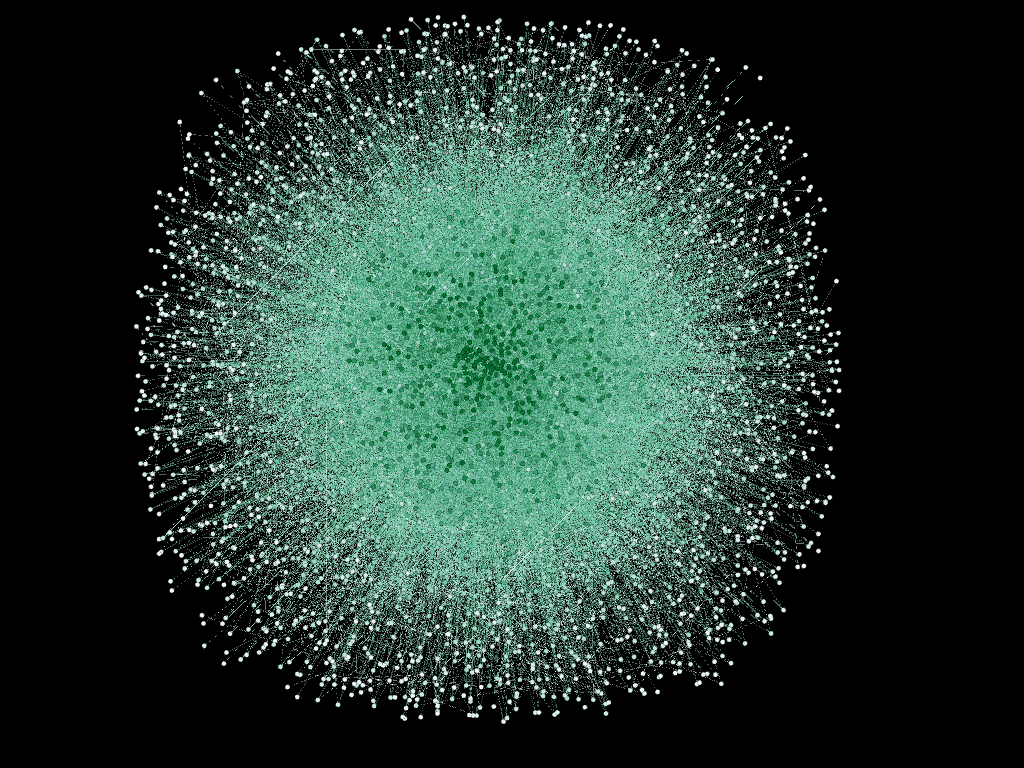
\includegraphics[width=16cm]{kcore.png}
\caption{Figure of 3457 PSP. Fruchterman Rheingold layout. Vertices coloured by coreness from dark green (high) to white (low). Coreness range 1-24. A central core is clearly seen in the physics based layout with a greater density of high kcore vertices. Gephi image in \url{~/Dropbox/stront_share/new_gephi/PSP_3457_coreness_Frucht_core_periphery.gephi
}}
\label{Fig:kcoreness}
\end{figure}

\todo{Calculate kcore correlation with p val - treat as a vertex index}



%\chapter{Phenotypes and the Post synaptic proteome network}
\section{Phenotypes considered}


\section{Intellectual disabilitity}
Intellectual disability and the genetics of intelligence. 
\section{Degree and id genes}
Examining the centrality measures for the 692 ID genes from cite(vissers2016genetic) implicated in intellectual disability,  245 are in the PSP.


 The median degree and mean degree are higher but not significantly so (Two sample Wilcoxon rank sum test with continuity correction - Mann-Whitney, W = 454524, p-value = 0.055 calculated in R) although the difference in the betweenness centrality is significant (Wilcoxon rank sum test with continuity correction. W = 467100, p-value = 0.006944, two sided for visser greater than W = 467100, p-value = 0.0032 ) see table \ref{table:degree_visser}, \ref{table:visser_betweenness}. \todo{90 centile degree for different diseases}
 
692 genes were identified from Visser et al 2016 Nature Review Genetics (ref) . The paper states there are ~700 genes and over 700 genes but I cannot identify a precise figure and the supplemental material is in PDF format and not machine readable.
692 genes were extracted using the python module pdf2text (ref) and confirming the list of genes gene identity in ToppGene (ref). These were stored as a pdf.
245 synaptic genes were identified. 35.4\% of the genes reported by Visser are synaptic and represent 7\% of the 3457 vertex PSP.  
There was no significant difference in degree distribution between ID genes and the PSP as a whole 
(median 10.0 Visser, 8 PSP, Mean 19.24 v 17.64 – Visser, p = 0.054 Wilcoxon test in R)
There was a significant difference in betweenness centrality (Median 317 v Median 540, p=0.006944 ) higher betweenness centrality. The genes appeared to be underrepresented as articulation points in the PSP (3 of 203)
Eigenvector similarity appears to be non significant

They are unevenly distributed with spectral clustering. The top group is group 4 with 9 of 31 genes associated. A high ranking GO term for group 4 is peroxisome related (8 genes). 7 of the 9 visser genes were associated with this GO term showing some modularity in function in at least a proportion of cases. Group 5 has 11 genes from Visser (9.2\% of community, slightly more than average of PSP).

Top groups spectral
\begin{table}[ht]
\centering
\begin{tabular}{clll}
\hline
 Spectral group &Freq visser& PSP group size &frac of group\\
              4&           9 &            31&    0.29\\
          47  &         6   &          27  &  0.222\\
          19   &        3    &         20   & 0.150\\
         45    &      15     &       124 &   0.121\\
           43     &     18      &      150  &  0.120\\
           22      &     5       &      42   & 0.119\\
         26       &   13      &      120 &   0.108\\
        28       &    4     &        38  &  0.105\\
            5      &    11    &        112   & 0.098\\
          24     &      7   &          76 &   0.092\\
\end{tabular}
\caption{Distribution of ID genes from Visser over spectral groups}
\label{table:Distribution of ID genesw from Visser over spectral groups}
\end{table}
  %from \hyperref{/home/grant/Dropbox/stront_share/PhD_bits/id}


% latex table generated in R 3.6.1 by xtable 1.8-4 package
% Mon Oct  7 13:54:07 2019
\begin{table}[ht]
\centering
\begin{tabular}{rrrrrrrr}
  \hline
 & Min. & 1st Qu. & Median & Mean & 3rd Qu. & Max. & n\\ 
  \hline
all\_synapse & 1.00 & 4.00 & 8.00 & 17.64 & 19.00 & 535.00 &3457\\ 
  visser synaptic & 1.00 & 4.00 & 10.00 & 19.24 & 22.00 & 263.00 & 245\\ 
   \hline
\end{tabular}
\caption{Difference in degree. PSP genes in cite(vissers2016genetic) p = 0.54}
\label{table:degree_visser}
\end{table}

% latex table generated in R 3.6.1 by xtable 1.8-4 package
% Mon Oct  7 14:08:05 2019
\begin{table}[ht]
\centering
\begin{tabular}{rrrrrrrr}
  \hline
 & Min. & 1st Qu. & Median & Mean & 3rd Qu. & Max. & n\\ 
  \hline


All PSP & 0.00 & 43.29 & 317.04 & 3421.08 & 1571.57 & 644670.69 & 3457 \\ 
  Visser genes & 0.00 & 68.94 & 540.62 & 3485.36 & 2761.75 & 85706.61 & 245\\ 
   \hline
\end{tabular}
\caption{Difference in betweenness centrality. PSP genes in citep(vissers2016genetic) p=0.0069}
\label{table:visser_betweenness}
\end{table}
cite(zabaneh2018genome)
\subsubsection{Essential genes and degree}
Lek
Database of essential genes. 


%\chapter{Orthologs}
\todo{Define ortholog}
\todo{Gene duplication}
\todo{Implications of barabasi model}
\section{Introduction}
Orthologous proteins in different species are those related by variation from the most recent common ancestor of the species \cite{fitch2000homology}. Paralogous genes originate from gene duplication rather than speciation and may occur in the same genome \cite{jensen2001orthologs}.

Hub nodes in orthologs are known to be more commonly associated with lethality \todo{ref} but it may be because of their involvement in processes intrinsic to the cell cycle that yeast nodes as a whole are more likely to be essential. 

The increase in the number of vertebrate synaptic genes following genome duplcation has allowed for greater evolutionary variation in function without lethality one thing that is known is (ref) that the synapse is pretty robust to mutations (ie it does not stop working completely) a source of robustness in addition to gene duplication may be network structure that allows convergent processes to occur. \todo{rephrase}
 
 Yeast mine \url{https://www.ncbi.nlm.nih.gov/pmc/articles/PMC5753351/}
 
\section{Methods}
\subsection{BioMart Orthologs}
Orthologs were extracted from Ensembl-EBI BioMart\cite{kinsella2011ensembl} for Genome Reference Consortium human (GRCh) 37 build equivalent to UCSC hg19. \url{https://grch37.ensembl.org/index.html} \todo{check ref for GRCh37} \cite{ramos2011validated}.
\url{https://www.ncbi.nlm.nih.gov/pmc/articles/PMC5753351/}
Data were downloaded from BioMart mapping Ensembl Gene ids (ENSG) and corresponding Ensembl transcript IDs (ENST)transcript id \url{https://www.ensembl.org/info/genome/genebuild/genome_annotation.html} to Entrez Gene GeneID \cite{maglott2005entrez} and Hugo Gene Name Committee (HGNC) symbol \cite{gray2012genenames}. Entrez Gene 'GeneID' had been used as the primary key when generating the post synaptic proteome network \todo{ref}. Only human genes with an orthogs were downloaded and orthologs from the taxa below were requested. The number of taxa exceeded the maximum in the BioMart portal and ortholog data were combined using a database join on human entrez gene GeneID. Data in \url{/home/grant/RProjects/orthologs2/biomart_37_orthologs}




\todo{Assortativity by ortholog}
It is suggested that 31\% of human genes have an ortholog in yeast \url{https://www.ncbi.nlm.nih.gov/pmc/articles/PMC3039837/} although the 

see also \url{https://www.ncbi.nlm.nih.gov/pmc/articles/PMC4012490/} Saccharomyces cerevisiae \url{https://science.sciencemag.org/content/274/5287/546} 6275 genes of which 5885 protein encoding

The following orthologs were downloaded applying the filter that only human genes with an ortholog would be present in the list (filter from biomart)

The following attributes were obtained for each ortholog and stored as a tsv file.

\begin{enumerate}
    
\item{Gene stable ID}
\item{Gene stable ID version}
\item{Transcript stable ID}
\item{Transcript stable ID version}
\item{other taxa gene stable ID}
\item{other taxa gene name}
\item{other taxa protein or transcript stable ID}
\item{other taxa chromosome/scaffold name}
\item{other taxa chromosome/scaffold start (bp)}
\item{other taxa chromosome/scaffold end (bp)}
\item{Query protein or transcript ID}
\item{Last common ancestor with other taxa}
\item{other taxa homology type}
%id. target other taxa gene identical to query gene
%id. query gene identical to target other taxa gene
\item{other taxa Gene-order conservation score}
\item{other taxa Whole-genome alignment coverage}
\item{dN with other taxa}
\item{dS with other taxa}
\item{other taxa orthology confidence [0 low, 1 high]}

\end{enumerate}
The following orthologs were downloaded:

\begin{itemize}
   
\item{Saccharomyces cerevisiae NCBI:txid4932}
\item{Caenorhabditis elegans NCBI:txid6239}
\item{Drosophila melanogaster NCBI:txid7227}
\item{Zebrafish Danio rerio NCBI:txid7955}
\item{Mouse Mus Musculus NCBI:txid10090}

\end{itemize}

A data frame mapping between Ensembl Gene id (ENSG), Hugo Gene Nomeclature Committee (HGNC) symbol and Entrez Gene GeneID was edited as follows:
\url{https://downloads.yeastgenome.org/genomics/homology/pdb_homologs/}
A dataframe of 233 397 rows was downloaded from BioMart (\url{source('~/RProjects/orthologs2/R/0_ensg2entrezbimap.R')}. The dataframe contained six columns:
\begin{itemize}
    \item Gene.stable.ID (ENSG)  
    \item Gene.stable.ID.version
    \item Transcipt.stable.ID (ENST)
    \item Transcript.stable.ID.version
    \item EntreGene.ID
    \item{HGNC symbol}
\end{itemize}           

The number of duplicated Gene.stable.id and Gene.stable.ID.version entries are identical (169720) and so Gene.stable.ID.version column could be dropped.

There were only 18227 duplicated transcript ID so the majority of the duplicated Gene.stable ID occured as a result of one ENSG id mapping to more than one ENST \todo{rephrase}. There were an identical number of duplicated transcript.id.version rows eg 18227 so the mapping of transcript and transcript id is one to one. 
 
As the primary key of the graph is Entrez GeneID all rows lacking Entrez Gene ID (recorded NA) were removed resulting in 190882 entries (42515 removed)\todo{find using entrez db cross ref}. Duplicate Entrez GeneIds were also removed to result in 25788 entries. Some Entrez Gene ID were not recorded by ensembl eg HMGA1P6 ENSG00000233440 is recorded as na but is at \url{https://www.ncbi.nlm.nih.gov/gene?cmd=Retrieve&dopt=full_report&list_uids=100130029} 100130029.It would be impracticable to find all missing. 

A second bimap was made of unique Gene Stable ID  27811, this contains 3358 duplicate entrez ids ie it is a one to many mapping GenestableID to Entrez
https://www.overleaf.com/project/5e19f349c1efb80001fbe76a
The unique entrez bimap has 1319 duplicated Gene.stable.ID ie ids that map to more than one entrez id.

These probably represent ids that have been retired at different rates. Looking at the duplicated gene stable id in the entrez bimap there are a number of duplicated gene symbols or missing gene symbols. What is important however is the number of duplicates in translation. As we are dealing with only those genes with orthologs we can check for duplicates

The entrez gene entry also maps to more than one ENSG on occasion. We want for each entrez to find an ortholog. 

\subsection{Methods for intermine}
Mod Enrichr \cite{kuleshov2019modenrichr} also provides a lookup service API for worm, fly, zebra fish and yeast model organisms based on data extracted from orthodb v 10 \cite{kriventseva2019orthodb} \todo{query add eggNOG} . However no API was apparent on the mod enrichr web site and while one was available for enrichr. The orthodb data consists of several database tables that are too large to fit in memory.

An alternative source of data is from yeast mine \cite{skrzypek2018saccharomyces} and related intermine sites which did not require the construction of a large database.

The PSP graph was annotated for ensembl id using yeast mine. This identified all 3457 genes from entrez id although 215 were not assigned ENSG ids. All were assigned HGNC standard names and all assigned to H. Sapiens taxa. A full descriptive gene name was not provided for 6 genes (look up in intermine \todo{do in R}. Initial annotation of the graph was done in 


1861 orthologs were identified in yeast mine for S. cerevisiae in the PSP. Mus  3341, Rattus 3238, Danio rerio 2623, Drosophila 1371, C elegans 1141.

There were 827 least diverged homologs for S.verevisiae. The total data frame including one to many was 6076 see table \ref{Table:Types of PSP orthology yeast mine}. Data is stored as \url{"~/RProjects/orthologs2/data_in/data_depot/ym_yeast_6076_all_ortho.tsv"}. We want to test the hypothesis that the scale free model of the PSP is consistent with the Barabasi-Albert model of network generation. That is that the phylogenetically older genes (most similar to earliest ancesteral forms) will have higher degree. The least diverged identified orthologs is a simplification of the development of the synaptic PSP but seems an  seem an appropriate measure and get round the problem of one to many mappings. 



\begin{table}{h}
\centering
\begin{tabular}{c|c}
   Homologue Type &	Count    \\
    \hline
    	orthologue 	&3,143 \\
    	homologue 	&1,779 \\
    	least diverged orthologue 	&827\\
    	horizontal gene transfer &	312\\
    	least diverged horizontal gene transfer 	&15\\
\end{tabular}
\caption{Types of PSP orthology - yeast mine}
\label{Table:Types of PSP orthology yeast mine}
\end{table}

1861 human orthologs are uniquely identified in the table. 1662 unique yeast genes.  

Least diverged 782 unique human gene symbol. 818 homologgenes, 808 homolog standard name.

0 genes in the least diverged category have no HGNC assigned but 76 have no ENSG (these will appear as duplicates of "") \url{source('~/RProjects/orthologs2/R/ym/yeast/parse_yeast_6076.R')}

We only have the network for human so do network interpretation and GSA for the 782  unique
\subsection{Results intermine}
785 human genes were identified using topp fun \todo{ref} (some duplicates) see \url{find_missing_yeast_hgnc_symbols.txt} in \url{/home/grant/RProjects/orthologs2/data_in/data_depot} for the PSP genes which had identifiable least diverged homologs in S. cerevisiae. 
\subsubsection{Graph analysis}
An induced subgraph on yeast ids makes 782 (removing the inaccurate duplicates). Largest connected subgraph 687. 

Summary stats degree

Min. 1st Qu.  Median    Mean 3rd Qu.    Max. 
   1.00    6.00   13.00   22.32   26.00  396.00 
   
   Compared with total 
   Min. 1st Qu.  Median    Mean 3rd Qu.    Max. 
   1.00    4.00    8.00   17.64   19.00  535.00 


The mean and median degree are greater for PSP proteins with identifiable least divergent yeast orthologs. There is a significant difference using a non parametric test of the centrality of the degree distribution (Wilcoxon rank sum test with continuity correction in R W = 1088858, p-value $< 2.2 x 10^{-16}$
alternative hypothesis: true location shift is not equal to 0). This would be consistent with the Barabasi-Albert hypothesis of preferential attachment with phylogenetically older nodes gaining more connections. The Barabasi-Albert model is a mechanism for the generation of scale free networks. 



see \url{source('~/RProjects/orthologs2/R/ym/yeast/yeast_subgraph.R')}

\todo{boxplot} 


\subsection{GO enrichment}
\subsection{Biological process}
Gene ontology enrichment was performed using the GO slim sets for Biological Process, Molecular Function and Cellular Component. Enrichment was calculated for the genes where there was a least divergent orthologue identified against a background of all PSP genes. 

As might be expected yeast orthologues are over-represented in processess such as ribosomal biogenesis.

Signal transduction is relatively under represented. 
% latex table generated in R 3.6.2 by xtable 1.8-4 package
% Sat Jan 25 15:21:45 2020
% latex table generated in R 3.6.2 by xtable 1.8-4 package
% Sat Jan 25 15:37:26 2020
\begin{sidewaystable}[ht]
\centering
\begin{adjustbox}{width=1\textwidth}
\small
\begin{tabular}{lrrrlrrr}
  \hline
GO Biological Process & Count PSP & Count yeast ortholog & Expected value & +/- & Fold change & P & FDR \\ 
  \hline
organic substance metabolic process (GO:0071704) & 804 & 303 & 199.360 & + & 1.5 & $1.71 \times 10^{-11}$ & $2.72 \times 10^{-8}$ \\ 
  metabolic process (GO:0008152) & 1031 & 365 & 255.640 & + & 1.4 & $5.20 \times 10^{-11}$ & $4.13 \times 10^{-8}$ \\ 
  macromolecule metabolic process (GO:0043170) & 520 & 212 & 128.940 & + & 1.6 & $2.47 \times 10^{-10}$ & $9.80 \times 10^{-8}$ \\ 
  translation (GO:0006412) & 115 & 75 & 28.510 & + & 2.6 & $2.28 \times 10^{-10}$ & $1.21 \times 10^{-7}$ \\ 
  translational elongation (GO:0006414) & 101 & 65 & 25.040 & + & 2.6 & $7.95 \times 10^{-9}$ & $1.80 \times 10^{-6}$ \\ 
  translational termination (GO:0006415) & 101 & 65 & 25.040 & + & 2.6 & $7.95 \times 10^{-9}$ & $2.10 \times 10^{-6}$ \\ 
  formation of translation initiation ternary complex (GO:0001677) & 101 & 65 & 25.040 & + & 2.6 & $7.95 \times 10^{-9}$ & $2.52 \times 10^{-6}$ \\ 
  gene expression (GO:0010467) & 391 & 151 & 96.950 & + & 1.6 & $2.46 \times 10^{-6}$ & $4.87 \times 10^{-4}$ \\ 
  ribonucleoprotein complex biogenesis (GO:0022613) & 34 & 27 & 8.430 & + & 3.2 & $1.32 \times 10^{-5}$ & $2.33 \times 10^{-3}$ \\ 
  cellular localization (GO:0051641) & 345 & 131 & 85.540 & + & 1.5 & $2.54 \times 10^{-5}$ & $3.10 \times 10^{-3}$ \\ 
  ribosome biogenesis (GO:0042254) & 28 & 24 & 6.940 & + & 3.5 & $2.48 \times 10^{-5}$ & $3.28 \times 10^{-3}$ \\ 
  protein modification by small protein conjugation (GO:0032446) & 76 & 43 & 18.840 & + & 2.3 & $3.51 \times 10^{-5}$ & $3.72 \times 10^{-3}$ \\ 
  protein modification by small protein conjugation or removal (GO:0070647) & 76 & 43 & 18.840 & + & 2.3 & $3.51 \times 10^{-5}$ & $3.99 \times 10^{-3}$ \\ 
  cellular protein localization (GO:0034613) & 313 & 119 & 77.610 & + & 1.5 & $5.79 \times 10^{-5}$ & $5.41 \times 10^{-3}$ \\ 
  cellular macromolecule localization (GO:0070727) & 313 & 119 & 77.610 & + & 1.5 & $5.79 \times 10^{-5}$ & $5.75 \times 10^{-3}$ \\ 
  proteasomal protein catabolic process (GO:0010498) & 52 & 32 & 12.890 & + & 2.5 & $8.94 \times 10^{-5}$ & $7.89 \times 10^{-3}$ \\ 
  protein ubiquitination (GO:0016567) & 72 & 40 & 17.850 & + & 2.2 & $9.91 \times 10^{-5}$ & $8.29 \times 10^{-3}$ \\ 
  proteasome-mediated ubiquitin-dependent protein catabolic process (GO:0043161) & 48 & 30 & 11.900 & + & 2.5 & $1.43 \times 10^{-4}$ & $1.04 \times 10^{-2}$ \\ 
  intracellular protein transport (GO:0006886) & 263 & 102 & 65.210 & + & 1.6 & $1.38 \times 10^{-4}$ & $1.04 \times 10^{-2}$ \\ 
  localization (GO:0051179) & 730 & 235 & 181.010 & + & 1.3 & $1.71 \times 10^{-4}$ & $1.13 \times 10^{-2}$ \\ 
  ribosomal small subunit biogenesis (GO:0042274) & 17 & 16 & 4.220 & + & 3.8 & $2.00 \times 10^{-4}$ & $1.22 \times 10^{-2}$ \\ 
  proteolysis involved in cellular protein catabolic process (GO:0051603) & 76 & 39 & 18.840 & + & 2.1 & $3.43 \times 10^{-4}$ & $2.01 \times 10^{-2}$ \\ 
  cellular protein catabolic process (GO:0044257) & 77 & 39 & 19.090 & + & 2.0 & $3.86 \times 10^{-4}$ & $2.19 \times 10^{-2}$ \\ 
  ncRNA metabolic process (GO:0034660) & 37 & 24 & 9.170 & + & 2.6 & $5.03 \times 10^{-4}$ & $2.66 \times 10^{-2}$ \\ 
  RNA metabolic process (GO:0016070) & 65 & 34 & 16.120 & + & 2.1 & $8.03 \times 10^{-4}$ & $3.87 \times 10^{-2}$ \\ 
  macromolecule catabolic process (GO:0009057) & 92 & 43 & 22.810 & + & 1.9 & $9.43 \times 10^{-4}$ & $4.28 \times 10^{-2}$ \\ 
  organelle assembly (GO:0070925) & 51 & 28 & 12.650 & + & 2.2 & $9.99 \times 10^{-4}$ & $4.41 \times 10^{-2}$ \\ 
   \hline
\end{tabular}
\end{adjustbox}
\caption{Gene Ontology Enrichment Slim PSP background for genes with identifiable least diverged yeast ortholog. Over represented terms} 
\label{Table: Gene Ontology Enrichment PSP background for genes with identifiable recent common ortholog. Over represented} 
\end{sidewaystable}
% latex table generated in R 3.6.2 by xtable 1.8-4 package
% Sat Jan 25 15:52:50 2020

\begin{sidewaystable}[ht]
\centering
\begin{adjustbox}{width=1\textwidth}
\small
\begin{tabular}{lrrrlrrr}

GO Biological Process & Count PSP & Count yeast ortholog & Expected value & +/- & Fold change & P & FDR \\ 
  \hline
multicellular organismal process (GO:0032501) & 380 & 53 & 94.220 & - & 0.6 & $1.89 \times 10^{-5}$ & $3.01 \times 10^{-3}$ \\ 
  Unclassified (UNCLASSIFIED) & 1736 & 354 & 430.450 & - & 0.8 & $2.46 \times 10^{-5}$ & $3.55 \times 10^{-3}$ \\ 
  multicellular organism development (GO:0007275) & 189 & 21 & 46.860 & - & 0.5 & $1.35 \times 10^{-4}$ & $1.07 \times 10^{-2}$ \\ 
  system development (GO:0048731) & 152 & 15 & 37.690 & - & 0.4 & $1.60 \times 10^{-4}$ & $1.11 \times 10^{-2}$ \\ 
  nervous system development (GO:0007399) & 119 & 10 & 29.510 & - & 0.3 & $1.97 \times 10^{-4}$ & $1.25 \times 10^{-2}$ \\ 
  regulation of signaling (GO:0023051) & 48 & 1 & 11.900 & - & 0.1 & $4.39 \times 10^{-4}$ & $2.40 \times 10^{-2}$ \\ 
  modulation of chemical synaptic transmission (GO:0050804) & 45 & 1 & 11.160 & - & 0.1 & $6.67 \times 10^{-4}$ & $3.31 \times 10^{-2}$ \\ 
  regulation of trans-synaptic signaling (GO:0099177) & 45 & 1 & 11.160 & - & 0.1 & $6.67 \times 10^{-4}$ & $3.42 \times 10^{-2}$ \\ 
  cell surface receptor signaling pathway (GO:0007166) & 231 & 32 & 57.280 & - & 0.6 & $8.75 \times 10^{-4}$ & $4.09 \times 10^{-2}$ \\ 
  cell communication (GO:0007154) & 180 & 23 & 44.630 & - & 0.5 & $1.23 \times 10^{-3}$ & $5.00 \times 10^{-2}$ \\ 
  signal transduction (GO:0007165) & 567 & 102 & 140.590 & - & 0.7 & $1.17 \times 10^{-3}$ & $5.01 \times 10^{-2}$ \\ 
  cell-cell signaling (GO:0007267) & 180 & 23 & 44.630 & - & 0.5 & $1.23 \times 10^{-3}$ & $5.13 \times 10^{-2}$ \\ 
   \hline
\end{tabular}
\end{adjustbox}
\caption{Gene Ontology Enrichment PSP background for genes with identifiable recent common ortholog under represented} 
\end{sidewaystable}
\todo{Split over and underrepresented and put portrait}
\subsection{Molecular function}
Over representation of ribosome and ribosomeal binding see table \ref{Table:Gene Ontology Molecular Function SLIM Enrichment PSP background for genes with identifiable recent common ortholog}

% latex table generated in R 3.6.2 by xtable 1.8-4 package
% Sat Jan 25 16:36:40 2020
\begin{table}[ht]
\centering
\begin{adjustbox}{width=1\textwidth}
\begin{tabular}{lrrrlrrr}
  \hline
GO Molecular Function & Count PSP & Count yeast ortholog & Expected value & +/- & Fold change & P & FDR \\ 
  \hline
structural constituent of ribosome (GO:0003735) & 80 & 64 & 19.840 & + & 3.2 & $1.70 \times 10^{-11}$ & $8.16 \times 10^{-9}$ \\ 
  structural molecule activity (GO:0005198) & 211 & 98 & 52.320 & + & 1.9 & $3.54 \times 10^{-7}$ & $8.48 \times 10^{-5}$ \\ 
  RNA binding (GO:0003723) & 193 & 91 & 47.860 & + & 1.9 & $5.86 \times 10^{-7}$ & $9.35 \times 10^{-5}$ \\ 
  heterocyclic compound binding (GO:1901363) & 409 & 144 & 101.410 & + & 1.4 & $2.10 \times 10^{-4}$ & $2.01 \times 10^{-2}$ \\ 
  nucleic acid binding (GO:0003676) & 387 & 136 & 95.960 & + & 1.4 & $3.56 \times 10^{-4}$ & $2.84 \times 10^{-2}$ \\ 
   \hline
\end{tabular}
\end{adjustbox}
\caption{Gene Ontology Molecular Function SLIM Enrichment PSP background for genes with identifiable recent common ortholog} 
\label{Table:Gene Ontology Molecular Function SLIM Enrichment PSP background for genes with identifiable recent common ortholog}
\end{table}
\subsection{Cellular component}
Over representation of cytosole and ribosome see table \ref{Table:Gene Ontology Cellular Conponent SLIM Enrichment PSP background for genes with identifiable recent common ortholog}

% latex table generated in R 3.6.2 by xtable 1.8-4 package
% Sat Jan 25 16:35:45 2020
\begin{table}[ht]
\centering
\begin{adjustbox}{width=1\textwidth}
\begin{tabular}{lrrrlrrr}
  \hline
GO Cellular Component & Count PSP & Count yeast ortholog & Expected value & +/- & Fold change & P & FDR \\ 
  \hline
cytoplasmic part (GO:0044444) & 758 & 319 & 187.950 & + & 1.7 & $1.52 \times 10^{-17}$ & $6.34 \times 10^{-15}$ \\ 
  cytosol (GO:0005829) & 303 & 161 & 75.130 & + & 2.1 & $5.32 \times 10^{-15}$ & $1.11 \times 10^{-12}$ \\ 
  intracellular part (GO:0044424) & 1217 & 435 & 301.760 & + & 1.4 & $2.70 \times 10^{-14}$ & $3.76 \times 10^{-12}$ \\ 
  cytosolic part (GO:0044445) & 98 & 74 & 24.300 & + & 3.0 & $2.03 \times 10^{-12}$ & $1.69 \times 10^{-10}$ \\ 
  cytoplasm (GO:0005737) & 1182 & 415 & 293.080 & + & 1.4 & $1.71 \times 10^{-12}$ & $1.79 \times 10^{-10}$ \\ 
  cytosolic ribosome (GO:0022626) & 72 & 59 & 17.850 & + & 3.3 & $4.19 \times 10^{-11}$ & $2.91 \times 10^{-9}$ \\ 
   \hline
\end{tabular}
\end{adjustbox}
\caption{Gene Ontology Cellular Conponent SLIM Enrichment PSP background for genes with identifiable recent common ortholog} 
\label{Table:Gene Ontology Cellular Conponent SLIM Enrichment PSP background for genes with identifiable recent common ortholog}
\end{table}

\subsection{Yeast murine phenotype}

Given the centrality of yeast orthologs to the cell cycle the PSP genes with orthologs in yeast are enriched for murine lethality embryonic lethality prior to organogenesis  MP:0013292 (Bonferroni $1.94 \times 10^{-28}$). See table \ref{Table:Mouse phenotype yeast ortholog PSPfor Bonferroni < 0.001}
% latex table generated in R 3.6.2 by xtable 1.8-4 package
% Sat Jan 25 17:01:27 2020
\begin{table}[ht]
\centering
\begin{adjustbox}{width=1\textwidth}
\begin{tabular}{llrrrr}
  \hline
Name & ID & Hit.Count.in.Query.List & Hit.Count.in.Genome & p.value & q.value.Bonferroni \\ 
  \hline
embryonic lethality prior to organogenesis & MP:0013292 & 123 & 875 & $4.94 \times 10^{-32}$ & $1.94 \times 10^{-28}$ \\ 
  preweaning lethality, complete penetrance & MP:0011100 & 159 & 1375 & $6.95 \times 10^{-32}$ & $2.73 \times 10^{-28}$ \\ 
  embryonic lethality prior to tooth bud stage & MP:0013293 & 128 & 976 & $2.38 \times 10^{-30}$ & $9.35 \times 10^{-27}$ \\ 
  embryonic lethality between implantation and placentation & MP:0009850 & 62 & 477 & $2.41 \times 10^{-14}$ & $9.46 \times 10^{-11}$ \\ 
  embryonic lethality between implantation and somite formation & MP:0006205 & 43 & 323 & $1.39 \times 10^{-10}$ & $5.46 \times 10^{-7}$ \\ 
  embryonic lethality, complete penetrance & MP:0011092 & 55 & 502 & $6.71 \times 10^{-10}$ & $2.63 \times 10^{-6}$ \\ 
  embryonic lethality between implantation and somite formation, complete penetrance & MP:0011096 & 36 & 293 & $3.97 \times 10^{-8}$ & $1.56 \times 10^{-4}$ \\ 
  abnormal embryonic growth/weight/body size & MP:0002088 & 92 & 1205 & $1.96 \times 10^{-7}$ & $7.72 \times 10^{-4}$ \\ 
  abnormal embryo development & MP:0001672 & 93 & 1226 & $2.24 \times 10^{-7}$ & $8.79 \times 10^{-4}$ \\ 
  abnormal prenatal growth/weight/body size & MP:0004196 & 103 & 1406 & $2.41 \times 10^{-7}$ & $9.45 \times 10^{-4}$ \\ 
   \hline
\end{tabular}
\end{adjustbox}
\caption{Mouse phenotype yeast ortholog PSP for Bonferroni $< 0.001$} 
\label{Table:Mouse phenotype yeast ortholog PSPfor Bonferroni < 0.001}
\end{table}
\subsection{Disease phenotype yeast ortholog}

Mitochondrial diseases are over represented bonferroni $2.11 \times 10^{-16}$. Amongst neurological disease Parkinson's disease is over represented  $1.53 \times 10^{-4}$. See table 
% latex table generated in R 3.6.2 by xtable 1.8-4 package
% Sat Jan 25 17:06:13 2020
\begin{table}[ht]
\centering
\begin{adjustbox}{width=1\textwidth}
\begin{tabular}{llrrrr}
  \hline
Name & ID & Hit.Count.in.Query.List & Hit.Count.in.Genome & p.value & q.value.Bonferroni \\ 
  \hline
Mitochondrial Diseases & C0751651 & 62 & 380 & $4.78 \times 10^{-20}$ & $2.11 \times 10^{-16}$ \\ 
  Aase Smith syndrome 2 & C2931850 & 15 & 19 & $8.47 \times 10^{-18}$ & $3.74 \times 10^{-14}$ \\ 
  HIV Coinfection & C4505456 & 25 & 102 & $7.59 \times 10^{-13}$ & $3.35 \times 10^{-9}$ \\ 
  Anemia, Diamond-Blackfan & C1260899 & 18 & 66 & $1.86 \times 10^{-10}$ & $8.23 \times 10^{-7}$ \\ 
  Parkinson Disease & C0030567 & 77 & 946 & $3.47 \times 10^{-8}$ & $1.53 \times 10^{-4}$ \\ 
  Cytopenia & C0010828 & 28 & 206 & $6.13 \times 10^{-8}$ & $2.71 \times 10^{-4}$ \\ 
  Congenital anemia & C0158995 & 28 & 208 & $7.55 \times 10^{-8}$ & $3.33 \times 10^{-4}$ \\ 
   \hline
\end{tabular}
\end{adjustbox}
\caption{Disease yeast ortholog PSP showing p Bonferroni $< 0.001$} 
\label{Table:Disease yeast ortholog PSP showing p Bonferroni < 0.001}
\end{table}

\section{C elegans - yeast mine}

1141 orthologs are returned representing 1141 unique human genes and 1302 c elegans genes. 

HGNC used to lookup entrez in toppfunn 1120 genes found. 1141 after substitute names identified (no duplicates)
\todo{Has more neural so need to do enrichment without background to show this ie background of all genome}

\section{Induced subgraph C elegans}

Largest connected component 1016, 126 components all others single N 1141 E 4710 

Min. 1st Qu.  Median    Mean 3rd Qu.    Max. 
    1.0     5.0    11.0    20.7    24.0   535.0 
> summary(deg)
   Min. 1st Qu.  Median    Mean 3rd Qu.    Max. 
   1.00    4.00    8.00   17.64   19.00  535.00 
   
	Wilcoxon rank sum test with continuity correction

data:  deg and degs
W = 1748061, p-value = 7.839e-09
alternative hypothesis: true location shift is not equal to 0

Significant difference in degree

\todo{boxplot}

Enrichment will be similar to yeast but with some neural elements which will show through in all genome. Need to look at diff too. 
649 entrez in celegans not in yeast
293 entrez in yeast not celegans

Union of both 1434. Intersection    492 

difference celegans gives abnormal synaptic transmission on toppfunn and seizures \url{source('~/RProjects/orthologs2/R/ym/celegans/get_difference_elegansyeast.R')}

in \url{celegans_yeast_toppfun_diff.txt} in dir \url{/home/grant/RProjects/orthologs2/data_in}


\subsection{Drosophila}

1371 genes in yeast mine orthologues

dataframe is 1457

1371 unique human genes with 1449 drosophila genes

1341 genes found from HGNC of data frame (1457 includes duplicates) on first pass

single duplicates found for missing other than Sept2 (Sept2 and Sep6) and MARS MARS and SLA2 will find these correctly when we map back to entrez gene to create subgraph

1372 genes now

to toppfun still overwhelmed by mitochondria and lethality need to check diff and do gene ontology

    in \url{/home/grant/RProjects/orthologs2/data_in}
    
    \url{emacs drosphila_misssing_hgnc.txt}
    and \url{emacs drosphila_entrez_hgnc_from_toppfunn.txt} are missing and duplicates and all ids
    ? seeing some difference in human phenotype
    
\subsubsection{GO}

BP slim vs PSP little

MF all no significant vs PSP

MF slim nil significant fly vs PSP

CC go ER signal transduction

CC go slim ER cytoplasmic part




\subsubsection{Fly graph}

 Min. 1st Qu.  Median    Mean 3rd Qu.    Max. 
   1.00    4.00    8.00   17.64   19.00  535.00 
   
  Min. 1st Qu.  Median    Mean 3rd Qu.    Max. 
   1.00    5.00   11.00   19.95   23.00  396.00 
   
   Wilcoxon rank sum test with continuity correction

data:  deg and degs
W = 2133124, p-value = 5.797e-08
alternative hypothesis: true location shift is not equal to 0

1371 nodes and 6522 edges

Largest connected component 1239. 128 components. 2 of 2, 1 of 1 and 1 of 1239 all rest 124 single. \todo{what are the singletons}
    
    1371 genes found from graph (1372 but one is x) - actually the write to clipboard function writes out the x
    

\subsubsection{Fly diff}
Diff fly and yeast

Fly not in yeast 786
Yeast not in fly 197 \todo{This may be from taking least divergent rather than just orthologs}

Union 1568
Intersection 585 

\subsubsection{Toppfun and go difference}

\textbf{Toppfunn}

More enriched for human hypertonia etc, mouse synaptic transmission and locomotion, cc synapse (toppfun)    bp purine bionucleotide and synaptic transmission

Disease epilepsy encephalopathy, mitochondria, schiz, epilepsy, NAD Co q deficiency

\textbf{GO}

BP diff translation PSP
MF complete nil significant
MF slim nil significant



\todo{pLI and orthologs}
\todo{Orthologs and coreness, eigenvector and betweeness}
\todo{Distribution over core periphery}


\section{Zebra fish}

Data frame returned from PSP conversion is 2932.

2623 unique human genes from PSP 
2921 orthologs identified in zebra fish

\section{Initial human orthologs to toppfun}
HGNC symbol in (output of yeast mine is HGNC, ENSG and orthologue gene identifier. 

2565 unique found on first pass Several not found find id more than one has two id.
This results in 2625 genes (excess will be mapped back when we use the graph to map entrez id. The txt files from toppfun are in \url{/home/grant/RProjects/orthologs2/data_in}
    
\subsection{Graph zebra fish}

PSP graph is 2622 vertices and 19702 edges. 48 components. Largest 2574. 1 component of 2. 46 singles. 

Degree PSP

 Min. 1st Qu.  Median    Mean 3rd Qu.    Max. 
   1.00    4.00    8.00   17.64   19.00  535.00 
   
Degree zfish
   
  
  
Min. 1st Qu.  Median    Mean 3rd Qu.    Max. 
1.00    4.00    9.00   18.66   20.00  535.00  
    
    No significant difference in degree in zebra fish
    
    
	Wilcoxon rank sum test with continuity correction

data:  deg and degs
W = 4402876, p-value = 0.05618
alternative hypothesis: true location shift is not equal to 0

2622 entrez id from graph to toppfun and GO
\subsection{Differences with others}
Genes found in zfish not in fly 1384

Genes found in fly not zfish 133

Union 2755

intersection 1238

code to put difference to clipboard \url{source('~/RProjects/orthologs2/R/ym/d_rerio/get_diff_zfish.R')}

1348 genes to toppfun

\subsection{Z fish fly difference toppfun}
Milder human phenotype on differences. MF cytoskeletal binding protein 

pathway axon guidance

disease ASD top, scz


\subsection{GO analysis}
do go analysis for difference



    


\section{Human fly differences}

There does not seem to be much human fly difference when you do GO analysis against PSP in terms of frequency from groups

Tried it again with yeast and the terms that come up are the purified terms which is why I keep getting ribosomes etc they are over represented in the yeast

No significant go slim BP and human/fly and MF slim is under representation of ribosome

CC slim under representation ribosome human and fly

\todo{Get a set of lists together and ask Colin to do topponto for disease}

\todo {diff rerio and fly}




\section{Results}
\subsection{Results BioMart}
There are 4037 Entrez Genes mapped to a yeast ortholog

\url{source('~/RProjects/orthologs2/R/yeast_orthologs.R')} 


the variable mart37\_yeast has 4037 levels of gene id suggesting there are 4037 human genes with identified orthologs in yeast in this download.

%and \url{mart37_yeast\$Gene.stable.ID} has 4037 levels.
%\texttt{mart37_yeastGene.stable.ID} has 4037 levels
We are also able to characterise by confidence score in biomart (0 low 1 high)
Yeast
690 high confidence PSP orthologs 19.96\% of PSP
\todo{Toppgene and then xtable output}
\url{source('~/RProjects/graph_analysis/R/make_annotated_gml.R')} has variable dataframe ortho with also booleans for each ortholog

448 low confidence PSP 

Total 1138 32.9\%

The high confidence yeast genes (ie yeast orthologs of PS

p = 0.01P) contain a substantial number of genes (n=101) involved in vesicle organisation BP: GO:0016050 (p Bonferroni = 1.997E-15). Performed in toppgene with backgroun as genome. 

Yeast genes are clearly essential. The top mouse phenotype was embryonic lethality (n= 100, genes MP:0008762, Bonferroni 3.94E-4).

Pathway analysis in reactome revealed that the top two enriched terms were Membrane trafficking ID 1269877, Bonferroni 2.276E-12 n=57 genes and ID 1269876 Vesicle-mediated transport Bonferroni 5.406E-11. The third topic is also of interest in terms of the development of the neurotransmitting mechanisms, 1427858 Reactome clathrin-mediated endocytosis Bonferroni 6.7E-8 n=22

Celegans
1101 C elegans genes high confidence
985 low confidence
2086 total

Molecular function of c elegans is enriched for GO:0032553, ribonucleotide binding, P Bonferroni 1.543E-62 n=305

Recognisable synaptic elements now appear in enrichment analysis of cellular compartment GO:0045202 synapse P Bonferroni 7.203E-75 n=270/1482, 
GO:0005739 mitochondrion, P Bonferroni 1.019E-74 N=306/1865


Mouse phenotype showed more advanced development but still lethality

1 
MP:0011100 
preweaning lethality, complete penetrance 

1.243E-15 
6.591E-12 
6.034E-11 
6.591E-12 
177 
1374

And abnormalities of synaptic vesicle morphology


p = 0.01

2 
MP:0004769 
abnormal synaptic vesicle morphology 

8.240E-12

p = 0.01 
2.186E-8 
2.001E-7 
4.372E-8 
23 
6

And of synaptic morphology and electrophysiology


4 
MP:0009538 
abnormal synapse morphology 

4.724E-10 
5.085E-7 
4.655E-6 
2.506E-6 
45 
228 
5 
MP:0002910 
abnormal excitatory postsynaptic currents 

4.793E-10 
5.085E-7 
4.655E-6 
2.543E-6 
35 
151


Gene families were enriched for L and S Ribosomes


729 
L ribosomal proteins 
genenames.org 
3.448E-19 
8.516

p = 0.01E-17 
5.185E-16 
8.516E-17 
23 
51 

2 
728 
S ribosomal proteins 
genenames.org 
2.321E-18 
2.867E-16 
1.745E-15 
5.733E-16 
19 
34


Human diseases included mitochondrial disease and neurodegenerative disorders


1 
C0751651 
Mitochondrial Diseases 
DisGeNET Curated 
1.065E-18 
6.017E-15 
5.546E-14 
6.017E-15 
73 
380 
2 
C0543888 
Epileptic encephalopathy 
DisGeNET Curated 
8.691E-12 
2.455E-8 
2.263E-7 
4.910E-8 
68 
459 
3 
C2931850 
Aase Smith syndrome 2 
DisGeNET Curated 
8.786E-11 
1.655E-7 
1.525E-6 
4.964E-7 
12 
19 
4 
C0524851 
Neurodegenerative Disorders 
DisGeNET Curated 
1.325E-9 
1.872E-6 
1.726E-5 
7.489E-6 
84 
695 
5 
C0086743 
Osteoarthrosis Deformans 
DisGeNET Curated 
1.024E-8 
1.157E-5 
1.066E-4 
5.784E-5 
22 
88

Drosophila

High confidence orthologs 1693 	48.9%
Low confidence orthologs 646	18.7%
Total 2339				67.65982%

Drosophila also show enrichment for ribonucleotide binding 
1 
GO:0032553 
ribonucleotide binding 

5.344E-96 
1.075E-92

p = 0.01 
8.794E-92 
1.075E-92 
454 
1947
And known synaptic components in cellular comparment


GO:0045202 
synapse 

5.004E-121 
6.360E-118 
4.913E-117 
6.360E-118 
410 
1482

Human phenotype is dominated by abnormalities of locomotion, abnormal muscle tone


HP:0003808 
Abnormal muscle tone 

1.961E-18 
1.009E-14 

p = 0.01
9.207E-14 
1.009E-14 
293 
1674

Mouse phenotype shows later lethality and some structural malformation


1 
MP:0011100 
preweaning lethality, complete penetrance 

4.216E-29 
2.695E-25 
2.517E-24 
2.695E-25 
287 
1374 
2 
MP:0008762 
embryonic lethality 

2.045E-19 
6.536E-16 
6.105E-15 
1.307E-15 
338 
1947 
3 
MP:0013293 
embryonic lethality prior to tooth bud stage 

3.457E-17 
7.365E-14 
6.879E-13 
2.209E-13 
189 
933 
4 
MP:0008540 
abnormal cerebral hemisphere morphology 

5.434E-17 
8.683E-14 
8.110E-13 
3.473E-13 
148 
668 
5 
MP:0013292 
embryonic lethality prior to organogenesis 

8.443E-17 
1.079E-13 
1.008E-12 
5.397E-13 
172 
827


Membrane trafficking is prominent in pathway analysis and almost all the components of SRP dependent contranslation are in place


1 
1269877 
Membrane Trafficking 
BioSystems: REACTOME 
1.678E-44 
4.605E-41 
3.912E-40 
4.605E-41 
196 
614 
2 
1269876 
Vesicle-mediated transport 
BioSystems: REACTOME 
4.888E-41 
6.706E-38 
5.696E-37 
1.341E-37 
199 
660

5 
1268689 
SRP-dependent cotranslational protein targeting to membrane 
BioSystems: REACTOME 
1.395E-31 
7.654E-29 
6.502E-28 
3.827E-28 
65 
116 
6 
1270303 
Axon guidance 
BioSystems: REACTOME 
5.388E-31 
2.464E-28 
2.093E-27 
1.478E-27 
161 
55

VEGFA-VEGFR2 Pathway 
BioSystems: REACTOME 
1.251E-27 
3.813E-25 
3.239E-24 
3.432E-24 
112 
333
9 above

Disease phenotype now shows a substantial amount of neurodegenerative


1 
C0751651 
Mitochondrial Diseases 
DisGeNET Curated 
6.405E-29 
4.811E-25 
4.571E-24 
4.811E-25 
112 
380 
2 
C0543888 
Epileptic encephalopathy 
DisGeNET Curated 
5.195E-23 


p = 0.011.951E-19 
1.854E-18 
3.902E-19 
115 
459 
3 
C0002395 
Alzheimer's Disease 
DisGeNET Curated 
2.767E-12 
6.929E-9 
6.583E-8 
2.079E-8 
259 
1819 
4 
C2931850 
Aase Smith syndrome 2 
DisGeNET Curated 
3.395E-11 
6.375E-8 
6.057E-7 
2.550E-7 
14 
19 
5 
C0030567 
Parkinson Disease 
DisGeNET Curated 
1.242E-10 
1.865E-7

p = 0.01 
1.772E-6 
9.327E-7 
150 
946


Taking the difference between drosophila and yeast 1004 genes

Mouse



MP:0002206 
abnormal CNS synaptic transmission 

4.019E-16 
2.325E-12 
2.149E-11 
2.325E-12 
124 
779 
2 
MP:0008540 
abnormal cerebral hemisphere morphology 

2.174E-15 
6.289E-12 
5.811E-11 
1.258E-11 
110 
668 
3 
MP:0003635 
abnormal synaptic transmission 

5.466E-15 
1.054E-11 
9.740E-11 
3.162E-11 
142 
977 
4 
MP:0000787 
abnormal telencephalon morphology 

6.676E-13 
9.258E-10 
8.555E-9 
3.862E-9 
127 
888 
5 
MP:0002882 
abnormal neuron morphology 

8.002E-13 
9.258E-10 
8.555E-9 
4.629E-9 
199 
1634

Human phenotype


1 
HP:0001290 
Generalized hypotonia 

1.196E-10 
5.535E-7 
4.991E-6 
5.535E-7 
106 
808 
2 
HP:0003808 
Abnormal muscle tone 

6.714E-10 
1.553E-6 
1.401E-5 
3.107E-6 
177 
1674 
3 
HP:0001276 
Hypertonia 

1.374E-8 
1.590E-5 
1.434E-4 
6.359E-5 
105 
863 
4 
HP:0001257 
Spasticity 

1.374E-8 
1.590E-5 
1.434E-4 
6.359E-5 
105 
863 
5 
HP:0001252 
Muscular hypotonia 

2.119E-8 
1.961E-5 
1.768E-4 
9.803E-5 
138 
1254

CC (need to do in panther)


1 
GO:0045202 
synapse 

1.061E-79 
1.147E-7

p = 0.016 
8.678E-76 
1.147E-76 
273 
1482 
2 
GO:0044456 
synapse part 

2.637E-75 
1.425E-72 
1.078E-71 
2.851E-72 
241 
1228 
3 
GO:0043005 
neuron projection 

3.265E-69 
1.177E-66 
8.899E-66 
3.530E-66 
271 
1624 
4 
GO:0098793 
presynapse 

5.209E-64 
1.408E-61 
1.065E-60 
5.631E-61 
167 
699 
5 
GO:0030424 
axon 

2.100E-54 
4.540E-52 
3.434E-51 
2.270E-51 
168 
817
Gene family



p = 0.01
1 
1150 
NADH:ubiquinone oxidoreductase supernumerary subunits 
genenames.org 
2.842E-15 
7.873E-13 
4.883E-12 
7.873E-13 
16 
30 
2 
1055 
Exocyst complex 
genenames.org 
2.456E-13 
3.401E-11 
2.110E-10 
6.802E-11 
9 
9 
3 
1220 
Membrane associated guanylate kinases|PDZ domain containing 
genenames.org 
1.642E-12 
1.516E-10 
9.407E-10 
4.549E-10 
29 
152 
4 
646 
Mitochondrial ribosomal proteins 
genenames.org 
1.402E-9 
8.977E-8 
5.569E-7 
3.883E-7 
18 
79 
5 
904 
Calcium voltage-gated channel subunits|Membrane associated guanylate kinases 
genenames.org 
1.620E-9 
8.977E-8 
5.569E-7 
4.489E-7 
11 
26

Disease


1 
C0543888 
Epileptic encephalopathy 
DisGeNET Curated 
8.645E-13 
4.916E-9 
4.534E-8 
4.916E-9 
70 
459 
2 
C0751651 
Mitochondrial Diseases 
DisGeNET Curated 
1.844E-9 
5.243E-6 
4.835E-5 
1.049E-5 
55 
380 
3 
C0036341 
Schizophrenia 
DisGeNET Curated 
4.440E-8 
8.416E-5 
7.763E-4 
2.525E-4 
145 
1537 
4 
C0524851 
Neurodegenerative Disorders 
DisGeNET Curated 
1.108E-7 
1.576E-4 
1.453E-3 
6.303E-4 
78 
695 
5 
C0002395 
Alzheimer's Disease 
DisGeNET Curated 
1.799E-7 
2.046E-4 
1.887E-3 
1.023E-3 
163 
1819


6 
C0005586 
Bipolar Disorder 
DisGeNET Curated 
2.786E-7 

p = 0.01
2.641E-4 
2.436E-3 
1.585E-3 
79 
723 
7 
C1838979 
MITOCHONDRIAL COMPLEX I DEFICIENCY 
DisGeNET Curated 
5.129E-7 
4.167E-4 
3.843E-3 
2.917E-3 
11 
29 
8 
C0014544 
Epilepsy 
DisGeNET Curated 
5.864E-7 
4.169E-4 
3.845E-3 
3.335E-3 
66 
578 
9 
C1527404 
Female Pseudo-Turner Syndrome 
DisGeNET Curated 
8.160E-7 
4.731E-4 
4.363E-3 
4.641E-3 
7 
11 
10 
C0557874 
Global developmental delay 
DisGeNET BeFree 
8.319E-7 
4.731E-4 
4.363E-3 
4.731E-3 
38 
266 
11 
C0002736 
Amyotrophic Lateral Sclerosis 
DisGeNET Curated 
2.410E-6 
1.246E-3 
1.149E-2 
1.371E-2 
67 
614 
12 
C1535926 
Neurodevelopmental Disorders 
DisGeNET Curated 
3.116E-6 
1.429E-3 
1.318E-2 
1.772E-2 
31 
20

So the neurological complex disorders are beginning to come in in the gap between yeast and drosophila



Difference between yeast and drosophila (n=1104)

MF
Glumatergic synapse comes in in pathway
Also cytoskeletal binding in MF
Less lethal murine phenotype
	
Pubmed has plenty of PSD

1 
GO:0003924 
GTPase activity 

2.284E-32 
3.590E-29 
2.850E-28 
3.590E-29 
137 
796 
2 
GO:0008092 
cytoskeletal protein binding 

2.348E-30 
1.845E-27 
1.465E-26 
3.691E-27 
159 
1061 
3 
GO:0032553 
ribonucleotide binding 

1.145E-28 
6.002E-26 
4.764E-25 
1.801E-25 
231 
1947 
4 
GO:0032555 
purine ribonucleotide binding 

5.359E-28 
2.106E-25 
1.672E-24 
8.425E-25 
228 
1930 
5 
GO:0017076 
purine nucleotide binding 

1.002E-27 
3.150E-25 
2.501E-24 
1.575E-24 
229 
1951

BP


1 
GO:0016050 
vesicle organization 

7.542E-43 
5.729E-39 
5.450E-38 
5.729E-39 
241 
1784 
2 
GO:0099536 
synaptic signaling 

3.008E-42 
1.142E-38 
1.087E-37 
2.285E-38 
161 
913 
3 
GO:0099537 
trans-synaptic signaling 

3.457E-41 
6.044E-38 
5.749E-37 
2.626E-37 
158 
900 
4 
GO:0007268 
chemical synaptic transmission 

3.978E-41 
6.044E-38 
5.749E-37 
3.022E-37 
157 
891 
5 
GO:0098916 
anterograde trans-synaptic signaling 

3.978E-41 
6.044E-38 
5.749E-37 
3.022E-37 
157 
891 
Show 45 more annotations


CC
1 
GO:0045202 
synapse 

1.061E-79 
1.147E-76 
8.678E-76 
1.147E-76 
273 
1482 
2 
GO:0044456 
synapse part 

2.637E-75 
1.425E-72 
1.078E-71 
2.851E-72 
241 
1228 
3 
GO:0043005 
neuron projection 

3.265E-69 
1.177E-66 
8.899E-66 
3.530E-66 
271 
1624 
4 
GO:0098793 
presynapse 

5.209E-64 
1.408E-61 
1.065E-60 
5.631E-61 
167 
699 
5 
GO:0030424 
axon 

2.100E-54 
4.540E-52 
3.434E-51 
2.270E-51 
168 
817


Human phenotype

1 
1269877 
Membrane Trafficking 
BioSystems: REACTOME 
8.339E-36 
1.964E-32 
1.638E-31 
1.964E-32 
137 
614 
2 
1269876 
Vesicle-mediated transport 
BioSystems: REACTOME 
7.545E-33 
8.884E-30 
7.411E-29 
1.777E-29 
138 
660 
3 
1268763 
Neuronal System 
BioSystems: REACTOME 
1.647E-27 
1.293E-24 
1.079E-23 
3.879E-24 
89 
351 
4 
1268766 
Transmission across Chemical Synapses 
BioSystems: REACTOME 
2.664E-25 
1.568E-22 
1.308E-21 
6.273E-22 
66 
218 
5 
213818 
Glutamatergic synapse 
BioSystems: KEGG 
1.779E-17 
8.381E-15 
6.991E-14 
4.190E-14 
39 
114


1 
HP:0001290 
Generalized hypotonia 

1.196E-10 
5.535E-7 
4.991E-6 
5.535E-7 
106 
808 
2 
HP:0003808 
Abnormal muscle tone 

6.714E-10 
1.553E-6 
1.401E-5 
3.107E-6 
177 
1674 
3 
HP:0001276 
Hypertonia 

1.374E-8 
1.590E-5 
1.434E-4 
6.359E-5 
105 
863 
4 
HP:0001257 
Spasticity 

1.374E-8 
1.590E-5 
1.434E-4 
6.359E-5 
105 
863 
5 
HP:0001252 
Muscular hypotonia 

2.119E-8 
1.961E-5 
1.768E-4 
9.803E-5 
138 
1254


Murine phenotype


1 
MP:0002206 
abnormal CNS synaptic transmission 

4.019E-16 
2.325E-12 
2.149E-11 
2.325E-12 
124 
779 
2 
MP:0008540 
abnormal cerebral hemisphere morphology 

2.174E-15 
6.289E-12 
5.811E-11 
1.258E-11 
110 
668 
3 
MP:0003635 
abnormal synaptic transmission 

5.466E-15 
1.054E-11 
9.740E-11 
3.162E-11 
142 
977 
4 
MP:0000787 
abnormal telencephalon morphology 

6.676E-13 
9.258E-10 
8.555E-9 
3.862E-9 
127 
888 
5 
MP:0002882 
abnormal neuron morphology 

8.002E-13 
9.258E-10 
8.555E-9 
4.629E-9 
199 
1634

Pathway

1 
1269877 
Membrane Trafficking 
BioSystems: REACTOME 
8.339E-36 
1.964E-32 
1.638E-31 
1.964E-32 
137 
614 
2 
1269876 
Vesicle-mediated transport 
BioSystems: REACTOME 
7.545E-33 
8.884E-30 
7.411E-29 
1.777E-29 
138 
660 
3 
1268763 
Neuronal System 
BioSystems: REACTOME 
1.647E-27 
1.293E-24 
1.079E-23 
3.879E-24 
89 
351 
4 
1268766 
Transmission across Chemical Synapses 
BioSystems: REACTOME 
2.664E-25 
1.568E-22 
1.308E-21 
6.273E-22 
66 
218 
5 
213818 
Glutamatergic synapse 
BioSystems: KEGG 
1.779E-17 
8.381E-15 
6.991E-14 
4.190E-14 
39 
114


Pubmed

2 
28671696 
Spatiotemporal profile of postsynaptic interactomes integrates components of complex brain disorders. 
Pubmed 
9.814E-154 
4.214E-149 
5.030E-148 
8.427E-149 
235 
928


Diseases


1 
C0543888 
Epileptic encephalopathy 
DisGeNET Curated 
8.645E-13 
4.916E-9 
4.534E-8 
4.916E-9 
70 
459 
2 
C0751651 
Mitochondrial Diseases 
DisGeNET Curated 
1.844E-9 
5.243E-6 
4.835E-5 
1.049E-5 
55 
380 
3 
C0036341 
Schizophrenia 
DisGeNET Curated 
4.440E-8 
8.416E-5 
7.763E-4 
2.525E-4 
145 
1537 
4 
C0524851 
Neurodegenerative Disorders 
DisGeNET Curated 
1.108E-7 
1.576E-4 
1.453E-3 
6.303E-4 
78 
695 
5 
C0002395 
Alzheimer's Disease 
DisGeNET Curated 
1.799E-7 
2.046E-4 
1.887E-3 
1.023E-3 
163 
1819


More cognitive diseases and this is drosophila

Zebra fish

High confidence

1068

Low confidence

2019

Total 3087


Mouse

High confidence 

3062

Low confidence

156

Diff high confidence

Mouse and fly difference

n=1447

MF cytoskeletal and actin bindingh
Increasingly mild himan phenotype and murine more to do with ep
Mouse LTP fifth along with abnormal morphology
MAGUK come in in gene family




GO:0008092 
cytoskeletal protein binding 

9.599E-68 
1.613E-64 
1.291E-63 
1.613E-64 
254 
1061 
2 
GO:0050839 
cell adhesion molecule binding 

2.215E-40 
1.860E-37 
1.489E-36 
3.721E-37 
137 
525 
3 
GO:0003779 
actin binding 

1.095E-37 
6.133E-35 
4.909E-34 
1.840E-34 
122 
451 
4 
GO:0044877 
protein-containing complex binding 

7.941E-30 
3.335E-27 
2.669E-26 
1.334E-26 
220 
1357 
5 
GO:0045296 
cadherin binding 

9.136E-27 
3.070E-24 
2.457E-23 
1.535E-23 
89 
338

Biological process


1 
GO:0007010 
cytoskeleton organization 

1.174E-68 
1.029E-64 
9.934E-64 
1.029E-64 
324 
1663 
2 
GO:0120036 
plasma membrane bounded cell projection organization 

5.797E-65 
2.541E-61 
2.453E-60 
5.081E-61 
332 
1790 
3 
GO:0030030 
cell projection organization 

2.872E-64 
8.392E-61 
8.103E-60 
2.518E-60 
335 
1828 
4 
GO:0032989 
cellular component morphogenesi1 1220 Membrane associated guanylate kinases|PDZ domain containing genenames.org 1.320E-25 4.514E-23 2.895E-22 4.514E-23 48 152s 

1.236E-52 
2.709E-49 
2.616E-48 
1.084E-48 
253 
1297 
5 
GO:0031175 
neuron projection development 

4.707E-50 
8.252E-47 
7.968E-46 
4.126E-46 
231 
1151


Cellular compartment


1 
GO:0045202 
synapse 

2.779E-97 
3.109E-94 
2.362E-93 
3.109E-94 
344 
1482 
2 
GO:0043005 
neuron projection 

4.021E-86 
2.250E-83 
1.709E-82 
4.499E-83 
345 
1624 
3 
GO:0030054 
cell junction 

2.315E-77 
8.636E-75 
6.561E-74 
2.591E-74 
298 
1352 
4 
GO:0120038 
plasma membrane bounded cell projection part 

6.667E-77 
1.492E-74 
1.134E-73 
7.460E-74 
349 
1784 
5 
GO:0044463 
cell projection part 

6.667E-77 
1.492E-74 
1.134E-73 
7.460E-74 
349 
1784 
Show 45 more annotations


Human Phenotype
1 
HP:0004305 
Involuntary movements 

1.500E-7 
7.447E-4 
6.767E-3 
7.447E-4 
116 
750 
2 
HP:0002072 
Chorea 

5.745E-6 
9.050E-3 
8.224E-2
2.852E-2 
37 
175 
3 
HP:0002460 
Distal muscle weakness 

8.931E-6 
9.050E-3 
8.224E-2
4.434E-2 
33 
151 
4 
HP:0025373 
Interictal EEG abnormality 

1.094E-5 
9.050E-3 
8.224E-2
5.430E-2
5 
5 
5 
HP:0040168 
Focal seizures, afebril 

1.094E-5 
9.050E-3 
8.224E-2
5.430E-2
5 
5

Murine


1 
MP:0002206 
abnormal CNS synaptic transmission 

1.208E-28 
7.547E-25 
7.032E-24 
7.547E-25 
180 
779 
2 
MP:0003635 
abnormal synaptic transmission 

9.018E-27 
2.818E-23 
2.626E-22 
5.636E-23 
205 
977 
3 
MP:0008415 
abnormal neurite morphology 

7.688E-19 
1.602E-15 
1.492E-14 
4.805E-15 
115 
490 
4 
MP:0002882 
abnormal neuron morphology 

3.087E-18 
4.823E-15 
4.494E-14 
1.929E-14 
268 
1634 
5 
MP:0002207 
abnormal long term potentiation 

7.531E-16 
9.414E-13 
8.771E-12 
4.707E-12 
70 
251


Pathway


1 
1270303 
Axon guidance 
BioSystems: REACTOME 
5.707E-24 
1.421E-20 
1.193E-19 
1.421E-20 
118 
554 
2 
1270302 
Developmental Biology 
BioSystems: REACTOME 
2.027E-19 
2.522E-16 
2.118E-15 
5.045E-16 
171 
1081 
3 
1427849 
Protein-protein interactions at synapses 
BioSystems: REACTOME 
9.935E-17 
8.243E-14 
6.922E-13 
2.473E-13 
32 
73 
4 
1268763 
Neuronal System 
BioSystems: REACTOME 
1.470E-14 
9.148E-12 
7.682E-11 
3.659E-11 
73 
351 
5 
1427850 
Interactions of neurexins and neuroligins at synapses 
BioSystems: REACTOME 
6.558E-14 
3.265E-11 
2.741E-10 
1.632E-10 
26 
59


Gene family


1 
1220 
Membrane associated guanylate kinases|PDZ domain containing 
genenames.org 
1.320E-25 
4.514E-23 
2.895E-22 
4.514E-23 
48 
152


Disease 


1 
C0036341 
Schizophrenia 
DisGeNET Curated 
3.168E-20 
2.617E-16 
2.511E-15 
2.617E-16 
218 
1537 
2 
C0004352 
Autistic Disorder 
DisGeNET Curated 
1.572E-18 
6.492E-15 
6.230E-14 
1.298E-14 
111 
601 
3 
C0002726 
Amyloidosis 
DisGeNET Curated 
8.755E-17 
2.410E-13 
2.313E-12 
7.230E-13 
133 
826 
4 
C0014544 
Epilepsy 
DisGeNET Curated 
7.543E-15 
1.557E-11 
1.495E-10 
6.230E-11 
100 
578 
5 
C0002395 
Alzheimer's Disease 
DisGeNET Curated 
7.167E-14 
9.995E-11 
9.592E-10 
5.919E-10 
225 
1819 
Show 45 more annotations


To do diff zebra fish and mouse (mouse is social)
gmt for these


%\chapter{Extra tables}



\section{Correlation of vertex measures and study p values}

%\listoftables
\begin{table}[h]{}
\centering

\begin{tabular}{llllllll}
Vertex statistic & Spearman's $\rho$ \& $\rho$ value & Study & Study type\\
\hline
Betweenness Centrality & 0.022 & 0.214 & CTG & Intelligence\textsubscript{Replication}\\
Betweenness Centrality & -0.034 & 0.049 & UKBB Intelligence & Intelligence\textsubscript{Discovery}\\
Betweenness Centrality & 0.015 & 0.389 & EA2 & Education\textsubscript{Replication}\\
Betweenness Centrality & -0.002 & 0.917 & UKBB Education & Education\textsubscript{Discovery}\\
Closeness Centrality & -0.007 & 0.671 & CTG & Intelligence\textsubscript{Replication}\\
Closeness Centrality & -0.008 & 0.649 & UKBB Intelligence & Intelligence\textsubscript{Discovery}\\
Closeness Centrality & -0.024 & 0.172 & EA2 & Education\textsubscript{Replication}\\
Closeness Centrality & -0.033 & 0.059 & UKBB Education & Education\textsubscript{Discovery}\\
Degree & 0.022 & 0.208 & CTG & Intelligence\textsubscript{Replication}\\
Degree & 0.011 & 0.532 & UKBB Intelligence & Intelligence\textsubscript{Discovery}\\
Degree & -0.007 & 0.689 & EA2 & Education\textsubscript{Replication}\\
Degree & -0.035 & 0.044 & UKBB Education & Education\textsubscript{Discovery}\\
Eigenvector centrality & -0.002 & 0.921 & CTG & Intelligence\textsubscript{Replication}\\
Eigenvector centrality & -0.008 & 0.655 & UKBB Intelligence & Intelligence\textsubscript{Discovery}\\
Eigenvector centrality & -0.031 & 0.073 & EA2 & Education\textsubscript{Replication}\\
Eigenvector centrality & -0.028 & 0.109 & UKBB Education & Education\textsubscript{Discovery}\\
Transitivity & -0.026 & 0.16 & CTG & Intelligence\textsubscript{Replication}\\
Transitivity & -0.013 & 0.467 & UKBB Intelligence & Intelligence\textsubscript{Discovery}\\
Transitivity & -0.001 & 0.949 & EA2 & Education\textsubscript{Replication}\\
Transitivity & 0.008 & 0.679 & UKBB Education & Education\textsubscript{Discovery}\\

\end{tabular}
\caption{Figure1:Paper Correlation of Graph statistics to gene p value in cohorts. Generated from word document using pandoc word is the paper supplemental for this figure}
\label{Figure:Figure1:Paper Correlation of Graph statistics to gene p value in cohorts}

\end{table}

\todo{Rename table \ref{Figure:Figure1:Paper Correlation of Graph statistics to gene p value in cohorts}}

\section{GSA results}
\textbf{Table 2: Gene set analysis of gene sets produced from graph communities showing discovery and replication cohorts for intelligence and educational attainment..} Sets with \emph{p}\textless{}0.05 in MAGMA-GSA shown for discovery cohorts. Sets with \emph{p} \textless{} 0.05 in MAGMA-GSA and GSEA tested in independent replication cohorts with MAGMA \emph{p} corrected for multiple comparisons using permutation FWER method in MAGMA.
\textbf{Intelligence cohorts}

%\begin{longtable}[h]{@{}lllll@{}}
\begin{table}[]
    \centering
    \begin{tabular}{c|c|c|c|c}
         Set & N GENES & BETA & P\_MAGMA & P\_GSEA\tabularnewline
\hline
10 & 146 & 0.19 & 0.008 & 0.085\tabularnewline
\textbf{5} & \textbf{106} & \textbf{0.22} & \textbf{0.014} & \textbf{\textless{}0.001}\tabularnewline
22 & 42 & 0.24 & 0.047 & 0.11\tabularnewline
    \end{tabular}
    \caption{Discovery Intelligence: GSA results UKBB intelligence - MAGMA and GSEA}
    \label{Table:Discovery Intelligence: GSA results UKBB intelligence - MAGMA and GSEA}
\end{table}





\begin{table}[]
    \centering
    \begin{tabular}{c|c|c|c|c}
        SET & N GENES & BETA & P MAGMA & P GSEA\tabularnewline
        \hline
\textbf{5} & \textbf{106} & \textbf{0.209} & \textbf{0.009} & \textbf{0.007}\tabularnewline
    \end{tabular}
    \caption{Replication Intelligence: GSA results CTG intelligence -- MAGMA and GSEA}
    \label{Table:Replication Intelligence: GSA results CTG intelligence -- MAGMA and GSEA}
\end{table}




\textbf{Education cohorts}
\begin{table}
    \centering
\begin{tabular}[]{llllll}
\toprule
SET & N GENES & BETA & P MAGMA & P GSEA\tabularnewline
\textbf{5} & \textbf{106} & \textbf{0.29} & \textbf{0.002} & \textbf{0.007}\tabularnewline
\textbf{53} & 386 & 0.11 & 0.015 & 0.29 *\tabularnewline
\textbf{22} & \textbf{42} & \textbf{0.27} & \textbf{0.035} & \textbf{0.018}\tabularnewline
\textbf{47} & \textbf{2
3} & \textbf{0.37} & \textbf{0.035} & \textbf{0.014}\tabularnewline
\bottomrule
\end{tabular}
\caption{Discovery Education: GSA results UKBB education - MAGMA and GSEA}
\label{Discovery Education: GSA results UKBB education - MAGMA and GSEA}
\end{table}

\begin{table}[]
    \centering
    \begin{tabular}[]{llllll}
\toprule
SET & N GENES & BETA & P MAGMA & P MAGMA CORRECTED & P GSEA\tabularnewline
\textbf{5} & \textbf{106} & \textbf{0.199} & \textbf{0.0147} & \textbf{0.046} & \textbf{0.028}\tabularnewline
\textbf{22} & 41 & 0.0873 & 0.25 & 0.5756 & 0.099\tabularnewline
\textbf{47} & 23 & -0.0526 & 0.599 & 0.9384 & 0.362\tabularnewline
\bottomrule


\end{tabular}
\caption{Replication Education: GSA results EA2 educational attainment-- MAGMA p,MAGMA corrected for multiple comparisons (FWER) and GSEA.}
\end{table}




\pagebreak
\section{GSA as longtable}

\subsection{Intelligence cohorts}
\begin{longtable}[h]{@{}lllll@{}}
\toprule
Set & N GENES & BETA & P\_MAGMA & P\_GSEA\tabularnewline
10 & 146 & 0.19 & 0.008 & 0.085\tabularnewline
\textbf{5} & \textbf{106} & \textbf{0.22} & \textbf{0.014} & \textbf{\textless{}0.00
1}\tabularnewline
22 & 42 & 0.24 & 0.047 & 0.11\tabularnewline
\bottomrule
\caption{Discovery Intelligence: GSA results UKBB intelligence - MAGMA and GSEA}
\label{Table:Discovery Intelligence: GSA results UKBB intelligence - MAGMA and GSEA}
\end{longtable}



\begin{longtable}[]{@{}lllll@{}}
\toprule
SET & N GENES & BETA & P MAGMA & P GSEA\tabularnewline
\textbf{5} & \textbf{106} & \textbf{0.209} & \textbf{0.009} & \textbf{0.007}\tabularnewline
\bottomrule
\caption{Replication Intelligence: GSA results CTG intelligence -- MAGMA and GSEA}
\label{Replication Intelligence: GSA results CTG intelligence -- MAGMA and GSEA}
\end{longtable}




\subsection{Education cohorts}

\begin{longtable}[]{@{}lllll@{}}
\toprule
SET & N GENES & BETA & P MAGMA & P GSEA\tabularnewline
\textbf{5} & \textbf{106} & \textbf{0.29} & \textbf{0.002} & \textbf{0.007}\tabularnewline
\textbf{53} & 386 & 0.11 & 0.015 & 0.29 *\tabularnewline
\textbf{22} & \textbf{42} & \textbf{0.27} & \textbf{0.035} & \textbf{0.018}\tabularnewline
\textbf{47} & \textbf{23} & \textbf{0.37} & \textbf{0.035} & \textbf{0.014}\tabularnewline
\bottomrule
\caption{Discovery Education: GSA results UKBB education - MAGMA and GSEA}
\label{Table:Discovery Education: GSA results UKBB education - MAGMA and GSEA}
\end{longtable}



\begin{longtable}[]{@{}llllll@{}}
\toprule
SET & N GENES & BETA & P MAGMA & P MAGMA CORRECTED & P GSEA\tabularnewline
\textbf{5} & \textbf{106} & \textbf{0.199} & \textbf{0.0147} & \textbf{0.046} & \textbf{0.028}\tabularnewline
\textbf{22} & 41 & 0.0873 & 0.25 & 0.5756 & 0.099\tabularnewline
\textbf{47} & 23 & -0.0526 & 0.599 & 0.9384 & 0.362\tabularnewline
\bottomrule
\caption{Replication Education: GSA results EA2 educational attainment-- MAGMA p,MAGMA corrected for multiple comparisons (FWER) and GSEA.}
\label{Table:Replication Education: GSA results EA2 educational attainment-- MAGMA p,MAGMA corrected for multiple comparisons (FWER) and GSEA.}
\end{longtable}

\textbf{Table 2: Gene set analysis of gene sets produced from graph communities showing discovery and replication cohorts for intelligence and educational attainment..} Sets with \emph{p}\textless{}0.05 in MAGMA-GSA shown for discovery cohorts. Sets with \emph{p} \textless{} 0.05 in MAGMA-GSA and GSEA tested in independent replication cohorts with MAGMA \emph{p} corrected for multiple comparisons using permutation FWER method in MAGMA.

% latex table generated in R 3.6.2 by xtable 1.8-4 package
% Thu Jan 30 15:52:30 2020
\begin{table}[ht]
\centering
\begin{tabular}{rllrlrrrrl}
  \hline
 & Study & Graph statistic & t & df & p & cor & CI lower & CI upper & Test \\ 
  \hline
1 & Intelligence Discovery & Degree & -0.75 & 3455 & 0.45 & -0.01 & -0.05 & 0.02 & Pearson's product-moment correlation \\ 
  2 & Intelligence Discovery & Betweenness & -0.32 & 3455 & 0.75 & -0.01 & -0.04 & 0.03 & Pearson's product-moment correlation \\ 
  3 & Intelligence Discovery & Eigenvector & -0.85 & 3455 & 0.40 & -0.01 & -0.05 & 0.02 & Pearson's product-moment correlation \\ 
  4 & Intelligence Discovery & Transitivity & 1.00 & 3151 & 0.31 & 0.02 & -0.02 & 0.05 & Pearson's product-moment correlation \\ 
  5 & Intelligence Replication & Degree & -0.75 & 3455 & 0.45 & -0.01 & -0.05 & 0.02 & Pearson's product-moment correlation \\ 
  6 & Intelligence Replication & Betweenness & -0.32 & 3455 & 0.75 & -0.01 & -0.04 & 0.03 & Pearson's product-moment correlation \\ 
  7 & Intelligence Replication & Eigenvector & -0.85 & 3455 & 0.40 & -0.01 & -0.05 & 0.02 & Pearson's product-moment correlation \\ 
  8 & Intelligence Replication & Transitivity & 1.00 & 3151 & 0.31 & 0.02 & -0.02 & 0.05 & Pearson's product-moment correlation \\ 
  9 & Education Discovery & Degree & -0.75 & 3455 & 0.45 & -0.01 & -0.05 & 0.02 & Pearson's product-moment correlation \\ 
  10 & Education Discovery & Betweenness & -0.32 & 3455 & 0.75 & -0.01 & -0.04 & 0.03 & Pearson's product-moment correlation \\ 
  11 & Education Discovery & Eigenvector & -0.85 & 3455 & 0.40 & -0.01 & -0.05 & 0.02 & Pearson's product-moment correlation \\ 
  12 & Education Discovery & Transitivity & 1.00 & 3151 & 0.31 & 0.02 & -0.02 & 0.05 & Pearson's product-moment correlation \\ 
  13 & Education Replication & Degree & -0.75 & 3455 & 0.45 & -0.01 & -0.05 & 0.02 & Pearson's product-moment correlation \\ 
  14 & Education Replication & Betweenness & -0.32 & 3455 & 0.75 & -0.01 & -0.04 & 0.03 & Pearson's product-moment correlation \\ 
  15 & Education Replication & Eigenvector & -0.85 & 3455 & 0.40 & -0.01 & -0.05 & 0.02 & Pearson's product-moment correlation \\ 
  16 & Education Replication & Transitivity & 1.00 & 3151 & 0.31 & 0.02 & -0.02 & 0.05 & Pearson's product-moment correlation \\ 
   \hline
\end{tabular}
\caption{Correlation of study gene level statistic with network statistics for cognate protein/gene in PSP using Pearson's product moment correlation. Code at \url{source('~/RProjects/paper_xls_latex/R/make_df_graph_stats_correlation.R')}}
\end{table}

% latex table generated in R 3.6.2 by xtable 1.8-4 package
% Fri Feb 14 12:31:13 2020
\begin{table}[ht]
\centering
\begin{tabular}{rrrrrr}
  \hline
 & degree & betweenness & transitivity & closeness & kcoreness \\ 
  \hline
degree & $2.2 \times 10^{-16}$ & $2.2 \times 10^{-16}$ & $2.2 \times 10^{-16}$ & $2.2 \times 10^{-16}$ & $2.2 \times 10^{-16}$ \\ 
  betweenness & $2.2 \times 10^{-16}$ & $2.2 \times 10^{-16}$ & $9.016 \times 10^{-1}$ & $2.2 \times 10^{-16}$ & $2.2 \times 10^{-16}$ \\ 
  transitivity & $2.2 \times 10^{-16}$ & $9.016 \times 10^{-1}$ & $2.2 \times 10^{-16}$ & $2.2 \times 10^{-16}$ & $2.2 \times 10^{-16}$ \\ 
  closeness & $2.2 \times 10^{-16}$ & $2.2 \times 10^{-16}$ & $2.2 \times 10^{-16}$ & $2.2 \times 10^{-16}$ & $2.2 \times 10^{-16}$ \\ 
  kcoreness & $2.2 \times 10^{-16}$ & $2.2 \times 10^{-16}$ & $2.2 \times 10^{-16}$ & $2.2 \times 10^{-16}$ & $2.2 \times 10^{-16}$ \\ 
   \hline
\end{tabular}
\caption{Correlation between vertex centrality measures for PSP. p values} 
\label{tab:Correlation between vertex centrality measures for PSP. p values}
\end{table}

\chapter{Discussion}

My principal aims with this thesis were two-fold: first to investigate the practicality of network based analysis of complex traits and to discover general  principles that are applicable to such analyses; second to use these analyses to better understand a specific complex trait (intelligence) which we believed would be appropriate for such analysis (see section~\ref{sec:Introduction intelligence} and specifically  \ref{sec:Intelligence intro usefulness of intelligence as phenotype}).

In this chapter I will summarise the findings of the thesis for both of these. I will then discuss the strengths and limitations of this analysis and outline future work. I will conclude with some more speculative observations on this work informed by my experience in carrying out this analysis.
\section{Discussion}
\subsection{Intelligence and Educational Ability}
We find that communities associated with metabotropic glutamate receptors and iontotropic ampa receptors are enriched for differences in intelligence and educational ability. These findings are found in discovery and replication cohorts and the findings become stronger in more recent studies that overlap with our discovery and replication cohorts but provide additional numbers. 
In the discovery and replication cohorts the enriched portions of the communities are not so much the receptors themselves but their neighbours, proteins that contribute to the macromolecular complexes the receptors are embedded in. This finding supports the analyses and hypotheses of Grant \cite{grant2012synaptopathies} and the early work of Pocklington and co-workers \cite{pocklington2006proteomes} in community detection. 

The more recent studies (Savage and EA3) show enrichment both of the receptor and their neighbours but a substantial amount of the enrichment is found in the neighbouring proteins. These are findings that would be missed in a standard gene set analysis approach and supports the utility of network based community gene set analysis as a method of analysing complex traits. 

For the discovery and replication cohorts the enriching proteins share few common biological themes found in Gene Ontology base gene set enrichment save for their proximity to receptor genes that are known to participate in glutamatergic neurotransmission. It is interesting to note that amongst the only findings within this group is an enrichment for neurogenesis. Hill found neurogenesis enriched in a large cohort for intelligence but that group was over 1000 genes in size, this group by contrast is 7 genes and enriches. 



This suggests that the combination of community based GSA and Gene Ontology analysis may provide a more detailed interrogation of ontology or topology defined areas of enrichment in complex traits. 


Vertex statistic and intelligence





One of the issues with the project is the continuing evolution of the synaptic maps and that we can only address two of these while they are in a continuous state of evolution. Indeed the map could be said to change with the outcome of each published synaptic proteomic study. The only way to produce anything was to freeze the data at points. Hopefully the code written to optimise the analysis will make more fluid analysis possible in the future.

Further directions will include looking at the synaptic proteome over the course of time. When moving from a trait such as intelligence to polygenic disorders that have different onsets in time then if we assume these to be synaptopathies we can expect different proteins to be expressed and this to correspond to the critical periods of the emergence of the disorder. For example neurodevelopmental disorders early, schizophrenia we would expect to occur around the time of peak onset of schizophrenia. We also know that the proteome varies across the brain and we will need to take this into account.

Future analyses may also be able to incorporate data on gene expression

One limitation is that we throw away approximately 50\% of the information from SNPs because they do not correspond to protein encoding genes. A way of incorporating genetic variants known to affect genes such as eQTLs would be helpful. 

Ideally given the continuous evolution of the map and the analysis we would have an online resource like the fly brain project that updates the findings in relatively constant times and publications to advise of major changes to the map or interface. 

The genes in the region of the afected groups are subjedt to experiment one could see if they in addition to others had a role in learning.

There are reasons to believe that the synaptic proteome is somewhat different from the general proteom and indeed that its network structure is particularly important as synaptic proteins inherently form modular units with specific functions. More phylogenetically ancient proeteins were not enriched for association for intelligence but the murine and zebrafish proteomes showed greater enrichment than the consensus proteome.

The change in GWAS size in the course of the study and the rapid change in nomenclature (for example the difficulty in translating the output of VEGAS Gene symbols to contemporary entrez show some of the factors that make the reproducibility of studies of this nature over time problematic. I have tried to minimise this by depositing all of the lookup and data information used in this project at the time it was m	EPHB2	EPH receptor B2
6146	RPL22	ribosomal protein L22
23557	SNAPIN	SNAP associated protein
2054	STX2	syntaxin 2
5127	CDK16	cyclin dependent kinase 16
2055	CLN8	CLN8 transmembrane ER and ERGIC protein
6154	RPL26	ribosomal protein L26
339983	NAT8L	N-acetyltransferase 8 like
9230	RAB11B	RAB11B, member RAS oncogene family
11280	SCN11A	sodium voltage-gated channel alpha subunit 11
2066	ERBB4	erb-b2 receptor tyrosine kinase 4
5138	PDE2A	phosphodiesterase 2A
3092	HIP1	huntingtin interacting protein 1
5142	PDE4B	phosphodiesterase 4B
83992	CTTNBP2	cortactin binding protein 2
55327	LIN7C	lin-7 homolog C, crumbs cell polarity complex component
8224	SYN3	synapsin III
1056	CEL	carboxyl ester lipase
9256	TSPOAP1	TSPO associated protein 1
41	ASIC1	acid sensing ion channel subunit 1
43	ACHE	acetylcholinesterase (Cartwright blood group)
11311	VPS45	vacuolar protein sorting 45 homolog
51248	PDZD11	PDZ domain containing 11
11315	PARK7	Parkinsonism associated deglycase
2099	ESR1	estrogen receptor 1
9267	CYTH1	cytohesin 1
5173ade (eg the complete entrez info, Pli etc) so that a snapshot of the crossmapping between terms is maintained. 

You also observe the phenomenon where small changes in modularity give rise to quite different graphs. Typically this is a result of the graph having a hierarchical structure and two communities a and b being vcombined. There are a few difficulties with this first it is at present very difficult to represent such a structure using the standard tools of graph visualisation and second if one is treating communuites as units that then undergo statistical tests we have to have some way of choosing the apporirate unit. In the Newman and Givan clustering algorithm the idivision stops when the optimal level of modularity has been achieved. I would sugggest that where a study would give rise to communitiesw which make clear sense in terms of an experiment such as a populatio study where there is only a small change in modularity trhat which gives rise to the mapping that has an additional correspondance to realisty should be preferred so long as the change in modularity is not too great. This therefore results in the question of what is too great. One ansewr might be to optinmise the likelihood of hte graph and the study jointly nand in order to do this one would need a stochastic block model, this would also allow one to incorporate information on other mesoscale generating processes within the graph such as core periphery strcuture.

Does not take into account also dynamic effects e.g. rules based modelling discuss this briefly and also spatial orientation within the larger synapse (functional organisation of post synaptic glutamate receptors MacGillavry

The study provides an outline for a network analysis of GWA studies of neuropsychiatric disorders with synaptic involvement. An analysis of vertex properties with gene level results, an analysis of the site of enrichment core or periphery, community enrichment analysis and topological subgroup analysis. 

Barabasi treats disease entities as homogeneous however the disease module even if it encompasses all genes involved in the disease may represent two or more distinct processes. For example with the exception of disorders where it is possible to identify a causative mutation, organism or tissue diagnosis then a disease is a constellation of physical findings and history and investigations which may arise from more than one albeit closely related source. There are examples where redefining the groups contained within a disease group have yielded better correlation with progression and prognosis. 

One issue with MAGMA GWA is the choice of a background set. In competitive testing we test enrichment against the rest of the genome rather than seeing if the set of genes themselves are associated. The PSP enriches for educational attainment and intelligence so as the sample size of the PSP approximates the size of the PSP the enrichment value will approach this as opposed to no enrichment if the group were to approach the size of the genome. 


Choice of clustering method. A wide variety of choices of clustering method were available. Some such as the newman and girvan betweenness method were prohibitively slow with large networks even using a highly parrallelised implementation. Others such as the greedy agglomerative method led to the domination of the clusterings by some large units and many small ones. The spin glass method is also attractive but it is hard to see how one can devise an experiment using it. There is at minimum one tune able parameter and this can take any integer value. This is useful in controlling the size of groups and one can achieve good functional enrichment but the question of the choice of parameter remains an open one. One could try to learn an appropriate hyperparameter but against what is ones objective function. Both CMcC and I(in the pilot study) used grid search with more precision in the case of CMcC but this leads to a combinatorial explosion of possible clusterings and this only takes into account the gamma parameter. I think that this method is much more useful for exploratory data analysis and once one has chosen a good gamma or cooling parameter perhaps based on functional classification then one can go on to ask questions of empirical population data. However there is a problem too with this, we have shown that	EPHB2	EPH receptor B2
6146	RPL22	ribosomal protein L22
23557	SNAPIN	SNAP associated protein
2054	STX2	syntaxin 2
5127	CDK16	cyclin dependent kinase 16
2055	CLN8	CLN8 transmembrane ER and ERGIC protein
6154	RPL26	ribosomal protein L26
339983	NAT8L	N-acetyltransferase 8 like
9230	RAB11B	RAB11B, member RAS oncogene family
11280	SCN11A	sodium voltage-gated channel alpha subunit 11
2066	ERBB4	erb-b2 receptor tyrosine kinase 4
5138	PDE2A	phosphodiesterase 2A
3092	HIP1	huntingtin interacting protein 1
5142	PDE4B	phosphodiesterase 4B
83992	CTTNBP2	cortactin binding protein 2
55327	LIN7C	lin-7 homolog C, crumbs cell polarity complex component
8224	SYN3	synapsin III
1056	CEL	carboxyl ester lipase
9256	TSPOAP1	TSPO associated protein 1
41	ASIC1	acid sensing ion channel subunit 1
43	ACHE	acetylcholinesterase (Cartwright blood group)
11311	VPS45	vacuolar protein sorting 45 homolog
51248	PDZD11	PDZ domain containing 11
11315	PARK7	Parkinsonism associated deglycase
2099	ESR1	estrogen receptor 1
9267	CYTH1	cytohesin 1
5173 often it is not the predominant ontology member in a group that is associated with the phenotype but an agglomeration of supporting proteins which often have little in common other than their close interrreaction with the ontology members found to be associated with a phenotype in animal studies. In pursuing a very 'pure' functional enrichment using gene ontology for example as ones objective function using methods that have tunable parameters one misses these associated proteins. 

\subsection{Community structure and choice of algorithm}

Although the summation constraint \todo{look up} may avoid the trivial modularity solution (putting all vertices in one module) it does not avoid the 'near trivial' situation such as cone community with 99\% of the nodes and another with 1\%. Pocklington used visual inspection to fine tune the initial clustering but this is difficult when we have large numbers of vertices and is a potential source of bias if we are doing inference for example using population data. Some clustering modalities such as spin glass allow control over the number of communities with the approximate influence of size but there is the problem of tunable paramaters. Other such as Louvain are heirarchical (CDM is too) but often the implementation does not allow access tro the heirarchy or one is back with the problem of choosing the division that looks right (ie the level in the height of the heurarchy) rather than maximising the modularity or likelihood with consequent problems in inference. 

The best pragmatic solution so far may be to choose a method that gives `pretty good` (with the earlier caveat about problems in looking for too pure a functional enrichment)ideally one without tubale parameters. 

In our experience of the synaptic proteom spectral clustering and Louvain perform well although the groups are rather large with Louvain. In the future especially with access to raw genotype data maximising the joint (improbability) of the population study and clustering may be effective ie we accept a small decrease in modularity if it is associated with a partition that makes sense of the study but then there is the question of how small the change in modularity can be. 



We need a way in which we can take into account that the pre and post synaptic areas are integrated eg some processes cross them and form cross synaptic modules and also that some genes are present in both compartments. It seems that the isolated post synaptic component is enriched for educational attainment but a number of the most significant genes are those seen in the PSP.

In considering the difference between disease modules and topological groups we must consider two possibilities. First for a complex trait we are looking at a topological area where genetic variation occurs across the population which may lead to a convergent phenotype. This is different from looking at the effects of the perturbation of an area of the graph on neighbouring or more distant nodes for example gene expression in a loss of function mutation. OMIM and Var contain both, genes implicated in disease that are up-regulated or found to have a causative role and those where there are specific germ line changes that predispose to the disease. The modular structure of the synapse and the effects of synaptic protein structure on function make it more likely that differences in neighbouring proteins will impact the overall function of a topological unit or the synapse than in for example a biological pathway where constituents are more separated in time than space and limiting factors may include quantity of reactants. We see in the study of core genes the effects that variations in these have in multi-system disorders, incompatibility with viability or disorders of cell cycle (which is an ancient system conserved from yeast)
\section{Non obvious takehomes for discussion}

For the presynaptic proteome education phenotypes enrich but the intelligence ones in general do not. 

\section{Further discussion}
Lack of different intelligence phenotypes e.g. fluid etc in large scale genomic studies compared with Hill et al. where the finding was for a single phenotype
\section{Further research}
Missing heritability and the impact of exome data
Make it easy to use like FUMA
How findings of GWAS extend to more rare diseases give example of drug induced psychosis or high intelligence

%\bibliography{references}
\printbibliography
\backmatter
\chapter{Notes}
\section{extra refs}


\subsection{Introduction synapses}
\textcolor{red}{review}
@article{humeau2019next,
  title={The next generation of approaches to investigate the link between synaptic plasticity and learning},
  author={Humeau, Yann and Choquet, Daniel},
  journal={Nature neuroscience},
  volume={22},
  number={10},
  pages={1536--1543},
  year={2019},
  publisher={Nature Publishing Group}
}

\subsection{centrality measures}
@article{valente2008correlated,
  title={How correlated are network centrality measures?},
  author={Valente, Thomas W and Coronges, Kathryn and Lakon, Cynthia and Costenbader, Elizabeth},
  journal={Connections (Toronto, Ont.)},
  volume={28},
  number={1},
  pages={16},
  year={2008},
  publisher={NIH Public Access}
}

@inproceedings{koschutzki2004comparison,
  title={Comparison of centralities for biological networks},
  author={Kosch{\"u}tzki, Dirk and Schreiber, Falk},
  booktitle={German Conference on Bioinformatics 2004, GCB 2004},
  year={2004},
  organization={Gesellschaft f{\"u}r Informatik eV}
}

@article{jalili2016evolution,
  title={Evolution of centrality measurements for the detection of essential proteins in biological networks},
  author={Jalili, Mahdi and Salehzadeh-Yazdi, Ali and Gupta, Shailendra and Wolkenhauer, Olaf and Yaghmaie, Marjan and Resendis-Antonio, Osbaldo and Alimoghaddam, Kamran},
  journal={Frontiers in Physiology},
  volume={7},
  pages={375},
  year={2016},
  publisher={Frontiers}
}

\subsection{communities}
\textcolor{red}{Over 1000 citations}
@article{porter2009communities,
  title={Communities in networks},
  author={Porter, Mason A and Onnela, Jukka-Pekka and Mucha, Peter J},
  journal={Notices of the AMS},
  volume={56},
  number={9},
  pages={1082--1097},
  year={2009}
}

\textcolor{red}{cited by 853}
@article{good2010performance,
  title={Performance of modularity maximization in practical contexts},
  author={Good, Benjamin H and De Montjoye, Yves-Alexandre and Clauset, Aaron},
  journal={Physical Review E},
  volume={81},
  number={4},
  pages={046106},
  year={2010},
  publisher={APS}
}

\textcolor{red}{citations 97}
@article{lewis2010function,
  title={The function of communities in protein interaction networks at multiple scales},
  author={Lewis, Anna CF and Jones, Nick S and Porter, Mason A and Deane, Charlotte M},
  journal={BMC systems biology},
  volume={4},
  number={1},
  pages={100},
  year={2010},
  publisher={Springer}
}

\textcolor{red}{cited by 8635}
@article{fortunato2010community,
  title={Community detection in graphs},
  author={Fortunato, Santo},
  journal={Physics reports},
  volume={486},
  number={3-5},
  pages={75--174},
  year={2010},
  publisher={Elsevier}
}

\textcolor{red}{cited by 457}
@article{lancichinetti2012consensus,
  title={Consensus clustering in complex networks},
  author={Lancichinetti, Andrea and Fortunato, Santo},
  journal={Scientific reports},
  volume={2},
  pages={336},
  year={2012},
  publisher={Nature Publishing Group}
}

\textcolor{red}{cited by 877}
@article{lancichinetti2011finding,
  title={Finding statistically significant communities in networks},
  author={Lancichinetti, Andrea and Radicchi, Filippo and Ramasco, Jos{\'e} J and Fortunato, Santo},
  journal={PloS one},
  volume={6},
  number={4},
  year={2011},
  publisher={Public Library of Science}
}

\subsection{multilayer networks}@article{humeau2019next,
  title={The next generation of approaches to investigate the link between synaptic plasticity and learning},
  author={Humeau, Yann and Choquet, Daniel},
  journal={Nature neuroscience},
  volume={22},
  number={10},
  pages={1536--1543},
  year={2019},
  publisher={Nature Publishing Group}
}

\textcolor{red}{cited by 1936}
@article{kivela2014multilayer,
  title={Multilayer networks},
  author={Kivel{\"a}, Mikko and Arenas, Alex and Barthelemy, Marc and Gleeson, James P and Moreno, Yamir and Porter, Mason A},
  journal={Journal of complex networks},
  volume={2},
  number={3},
  pages={203--271},
  year={2014},
  publisher={Oxford University Press}
}

\textcolor{red}{over 100 pages, cited by 1878}
@article{boccaletti2014structure,
  title={The structure and dynamics of multilayer networks},
  author={Boccaletti, Stefano and Bianconi, Ginestra and Criado, Regino and Del Genio, Charo I and G{\'o}mez-Gardenes, Jes{\'u}s and Romance, Miguel and Sendina-Nadal, Irene and Wang, Zhen and Zanin, Massimiliano},
  journal={Physics Reports},
  volume={544},
  number={1},
  pages={1--122},
  year={2014},
  publisher={Elsevier}
}

New has modularity of real world networks

@article{zhang2009big,
  title={A big world inside small-world networks},
  author={Zhang, Zhihua and Zhang, Jianzhi},
  journal={PloS one},
  volume={4},
  number={5},
  year={2009},
  publisher={Public Library of Science}
}

cited by 1044

@article{brandes2007modularity,
  title={On modularity clustering},
  author={Brandes, Ulrik and Delling, Daniel and Gaertler, Marco and Gorke, Robert and Hoefer, Martin and Nikoloski, Zoran and Wagner, Dorothea},
  journal={IEEE transactions on knowledge and data engineering},
  volume={20},
  number={2},
  pages={172--188},
  year={2007},
  publisher={IEEE}
}


\subsection{general notes}
Wagner and Fell small world

\subsection{extra results}
Enrichment of new graph components


 MEAN SAMPLE\ SIZE = 250000
 TOTAL GENES = 18673
 CONDITIONED INTERNAL = genesize, log genesize, genedensity, log genedensity, inverse mac, log inverse mac
SET           NGENES       BETA   BETA STD         SE            P
new in graph    1397     0.0553     0.0145     0.0293     0.029806
new graph       4414      0.101     0.0427     0.0186   3.1989e-08
PSD             3414      0.113     0.0436     0.0201   1.0565e-08



\section{Readme from Sniekers}
\label{sec:notes readme from sniekers}

Uses NCBI 37.3 in MAGMA

     Association results of the meta-analysis for intelligence based on 78,308 individuals in 13 cohorts. 
     Version date: 10-07-2017

  Columns:
Chromosome: chromosome number
position: base pair position of the SNP on the chromosome (reported on GRCh37)
rsid: SNP rs number
ref: effect allele
alt: non-effect allele
N: sample size
MAF: minor allele frequency in UK Biobank
Beta: effect size of the effect allele
SE: standard error of the effect
Zscore: Z-score computed in METAL by a weighted Z-score method
p   value: P-value computed in METAL by a weighted Z-score method
direction: direction of the effect in each of the cohorts, order: CHIC (consisting of 6 cohorts), UKB-wb, UKB-ts, ERF, GENR, HU, MCTFR, STR

Beta/SE were calculated from METAL Z-scores using the formula from Zhu et al (Nature Genetics, 2016):

Beta = Zscore / sqrt( 2 * MAF * ( 1 - MAF) * ( N + $Zscore^2$ ) )
SE = 1 / sqrt( 2 * MAF * ( 1 - MAF ) * ( N + $Zscore^2$ ) )

\section{Useful papers for methods}

MDD for quoting MAGMA \url{https://www.nature.com/articles/s41467-018-03819-3}

\section{Literature for centrality and other stuff}
\label{sec:literature centrality and other stuff}
Shim \cite{shim2017gwab} reports GWAB a method for prioritising GWAS statistics given network structure. It uses a guilt by association method to increase the score of nodes which are neighbours of high scoring GWAS nodes. The gene level score comes from the highest scoring SNP rather than from VEGAS !(this is 2017). The network is taken from HumanNet a previous work by the authors \cite{lee2011prioritizing} (this one is cited by over 500). Human net incorporates "diverse distinct lines of evidence" including PPI, mRNA co-expression, comparative genomics data from yeast, fly and worm to result in a network with 16243 nodes and 476399 'scored functional couplings' which I take to be a weighted edge. Again this paper is GWAS boosting from guilt by association. 21 proteomic and genomic datasets were integrated from the four species (I assume human is the other along with yeast fly and worm). They also talk about markov clustering and GeneMania. In the construction bit they talk about training the network using gene ontology pairs again I am a bit lost with these.  

\section{Community detection}

Communities allow the network to be broken up into smaller components which can be analysed in turn and which may represent functional units.


\section{Modularity}
\label{sec:modularity definition}

for an adjacency matrix $A_{ij}$ we want to know how many edges pass between similar nodes that share a property be it an ontology term or a community membership.

Total number of edges is between nodes of same group is:

\begin{equation}
\label{eq:notes_modularity_totaledges}
    \frac{1}{2} \sum_{i,j} A_{i,j}\delta_{g_i g_j}
\end{equation}

The expected number of edges between all nodes of the same type is 

\begin{equation}
    \frac{1}{2}\sum_{i,j} \frac{k_i k_j}{2m}\delta_{g_i g_j}
\end{equation}

The modularity Q is 

\begin{equation}
    Q=\frac{1}{2m}\sum_{i,j}\textcolor{red}{(A_{i,j}-\frac{k_i k_j}{2m}}) \delta{g_i g_j}
\end{equation}

The red term is:

\begin{equation}
    B_{ij} = \sum_{i,j} A_{i,j} - \frac{k_i k_j}{2m}
\end{equation}

$\mathbf{B}$ is the modularity matrix which is n by n having elements $B_{i,j}$

\section{Simple example of spectral graph partitioning}
\label{sec:simple example of spectral graph partitioning}

Using the first eigenvector of the modularity matrix results in a partition with modularity 0.21. The distribution of the first four eigenvectors can be seen in figure~\ref{fig:simple example of spectral clustering}.\todo{?remove size for fourth}

Gene ontology analysis shows that the groups are quite different one of 1111 members linked to mRNA processing and biosynthesis see tables~\ref{tab:1111 group generated from sign of first eigenvector of modularity matrix. Biological function} compared with the genome and \ref{tab:1111 group generated from sign of first eigenvector of modularity matrix background PSP. Biological function. Alpha = 5.22520639565263e-06} compared with the rest of the PSP. The other group is of 2346 genes linked to trans-synaptic signalling see tables~\ref{tab:2346 group generated from sign of first eigenvector of modularity matrix. Biological function} and with background of PSP genes ~\ref{tab:2346 group generated from sign of first eigenvector of modularity matrix background PSP. Biological function. Alpha = 5.22520639565263e-06}
\begin{figure}
    \centering
    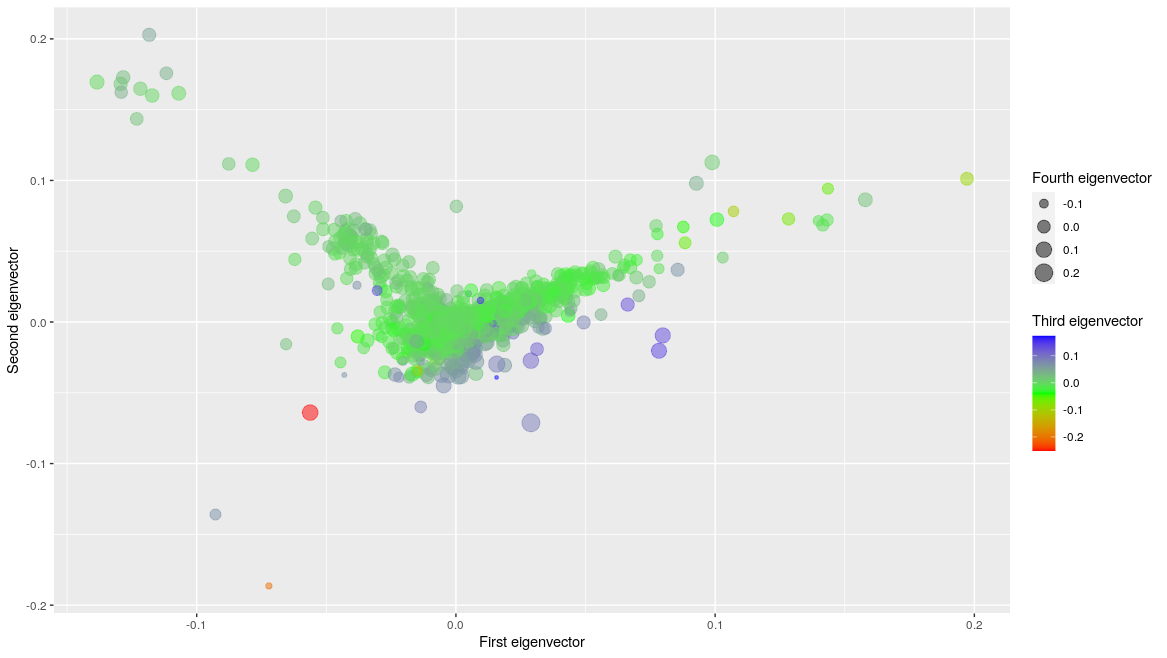
\includegraphics[width=\textwidth]{images/Rplot_eigenvectors_of_PSP_modularity_matrix.png}
    \caption{Simple example of spectral clustering of the PSP. The values of the $i$th entries of the first and second eigenvector are plotted on the x axis.}
    \label{fig:simple example of spectral clustering}
\end{figure}

% Sat May 16 14:53:46 2020
\begin{table}[ht]
\centering
\begin{tabular}{llrrrr}
  \hline
GO.ID & Term & Annotated & Significant & Expected & classic \\ 
  \hline
GO:0034641 & cellular nitrogen compound metabolic pro... & 1208 & 621 & 393.5 & $1.00 \times 10^{-30}$ \\ 
  GO:0016071 & mRNA metabolic process & 254 & 210 & 82.7 & $1.00 \times 10^{-30}$ \\ 
  GO:0010467 & gene expression & 922 & 506 & 300.3 & $1.00 \times 10^{-30}$ \\ 
  GO:0090304 & nucleic acid metabolic process & 801 & 452 & 260.9 & $1.00 \times 10^{-30}$ \\ 
  GO:0044271 & cellular nitrogen compound biosynthetic ... & 900 & 490 & 293.2 & $1.00 \times 10^{-30}$ \\ 
  GO:0043604 & amide biosynthetic process & 297 & 225 & 96.8 & $1.00 \times 10^{-30}$ \\ 
  GO:0006412 & translation & 258 & 204 & 84.0 & $1.00 \times 10^{-30}$ \\ 
  GO:0043043 & peptide biosynthetic process & 262 & 205 & 85.3 & $1.00 \times 10^{-30}$ \\ 
  GO:0034645 & cellular macromolecule biosynthetic proc... & 803 & 447 & 261.6 & $1.00 \times 10^{-30}$ \\ 
  GO:0009059 & macromolecule biosynthetic process & 830 & 456 & 270.4 & $1.00 \times 10^{-30}$ \\ 
  GO:0046483 & heterocycle metabolic process & 1076 & 549 & 350.5 & $1.00 \times 10^{-30}$ \\ 
  GO:0006139 & nucleobase-containing compound metabolic... & 1050 & 537 & 342.0 & $1.00 \times 10^{-30}$ \\ 
  GO:0016070 & RNA metabolic process & 716 & 407 & 233.2 & $1.00 \times 10^{-30}$ \\ 
  GO:1901360 & organic cyclic compound metabolic proces... & 1121 & 562 & 365.2 & $1.00 \times 10^{-30}$ \\ 
  GO:0006725 & cellular aromatic compound metabolic pro... & 1088 & 549 & 354.4 & $1.00 \times 10^{-30}$ \\ 
  GO:0006401 & RNA catabolic process & 179 & 152 & 58.3 & $1.00 \times 10^{-30}$ \\ 
  GO:0006402 & mRNA catabolic process & 175 & 149 & 57.0 & $1.00 \times 10^{-30}$ \\ 
  GO:1901576 & organic substance biosynthetic process & 1147 & 564 & 373.6 & $1.00 \times 10^{-30}$ \\ 
  GO:0009058 & biosynthetic process & 1160 & 568 & 377.9 & $1.00 \times 10^{-30}$ \\ 
  GO:0043603 & cellular amide metabolic process & 368 & 248 & 119.9 & $1.00 \times 10^{-30}$ \\ 
   \hline
\end{tabular}
\caption{1111 group generated from sign of first eigenvector of modularity matrix. Biological function} 
\label{tab:1111 group generated from sign of first eigenvector of modularity matrix. Biological function}
\end{table}

% latex table generated in R 3.6.3 by xtable 1.8-4 package
% Sat May 16 14:55:07 2020
\begin{table}[ht]
\centering
\begin{tabular}{llrrrr}
  \hline
GO.ID & Term & Annotated & Significant & Expected & classic \\ 
  \hline
GO:0030030 & cell projection organization & 572 & 483 & 385.7 & $7.80 \times 10^{-24}$ \\ 
  GO:0120036 & plasma membrane bounded cell projection ... & 566 & 478 & 381.6 & $1.40 \times 10^{-23}$ \\ 
  GO:0099537 & trans-synaptic signaling & 316 & 281 & 213.1 & $1.30 \times 10^{-20}$ \\ 
  GO:0023052 & signaling & 1510 & 1142 & 1018.1 & $1.50 \times 10^{-20}$ \\ 
  GO:0007268 & chemical synaptic transmission & 310 & 276 & 209.0 & $2.00 \times 10^{-20}$ \\ 
  GO:0098916 & anterograde trans-synaptic signaling & 310 & 276 & 209.0 & $2.00 \times 10^{-20}$ \\ 
  GO:0007154 & cell communication & 1508 & 1140 & 1016.8 & $2.30 \times 10^{-20}$ \\ 
  GO:0099536 & synaptic signaling & 318 & 282 & 214.4 & $2.90 \times 10^{-20}$ \\ 
  GO:0051049 & regulation of transport & 623 & 511 & 420.1 & $2.10 \times 10^{-19}$ \\ 
  GO:0007399 & nervous system development & 772 & 617 & 520.5 & $2.20 \times 10^{-18}$ \\ 
  GO:0048666 & neuron development & 439 & 368 & 296.0 & $9.30 \times 10^{-17}$ \\ 
  GO:0030029 & actin filament-based process & 333 & 287 & 224.5 & $1.70 \times 10^{-16}$ \\ 
  GO:0030036 & actin cytoskeleton organization & 284 & 249 & 191.5 & $2.10 \times 10^{-16}$ \\ 
  GO:0050804 & modulation of chemical synaptic transmis... & 218 & 197 & 147.0 & $2.20 \times 10^{-16}$ \\ 
  GO:0031175 & neuron projection development & 404 & 340 & 272.4 & $5.30 \times 10^{-16}$ \\ 
  GO:0099177 & regulation of trans-synaptic signaling & 219 & 197 & 147.7 & $7.50 \times 10^{-16}$ \\ 
  GO:0032879 & regulation of localization & 853 & 667 & 575.1 & $1.20 \times 10^{-15}$ \\ 
  GO:0032989 & cellular component morphogenesis & 453 & 375 & 305.4 & $3.00 \times 10^{-15}$ \\ 
  GO:0030182 & neuron differentiation & 478 & 393 & 322.3 & $5.10 \times 10^{-15}$ \\ 
  GO:0048699 & generation of neurons & 515 & 420 & 347.2 & $7.00 \times 10^{-15}$ \\ 
   \hline
\end{tabular}
\caption{2346 group generated from sign of first eigenvector of modularity matrix. Biological function} 
\label{tab:2346 group generated from sign of first eigenvector of modularity matrix. Biological function}
\end{table}

% latex table generated in R 3.6.3 by xtable 1.8-4 package
% Sat May 16 14:59:26 2020
\begin{table}[ht]
\centering
\begin{tabular}{llrrrr}
  \hline
GO.ID & Term & Annotated & Significant & Expected & classic \\ 
  \hline
GO:0030030 & cell projection organization & 572 & 483 & 385.7 & $7.80 \times 10^{-24}$ \\ 
  GO:0120036 & plasma membrane bounded cell projection ... & 566 & 478 & 381.6 & $1.40 \times 10^{-23}$ \\ 
  GO:0099537 & trans-synaptic signaling & 316 & 281 & 213.1 & $1.30 \times 10^{-20}$ \\ 
  GO:0023052 & signaling & 1510 & 1142 & 1018.1 & $1.50 \times 10^{-20}$ \\ 
  GO:0007268 & chemical synaptic transmission & 310 & 276 & 209.0 & $2.00 \times 10^{-20}$ \\ 
  GO:0098916 & anterograde trans-synaptic signaling & 310 & 276 & 209.0 & $2.00 \times 10^{-20}$ \\ 
  GO:0007154 & cell communication & 1508 & 1140 & 1016.8 & $2.30 \times 10^{-20}$ \\ 
  GO:0099536 & synaptic signaling & 318 & 282 & 214.4 & $2.90 \times 10^{-20}$ \\ 
  GO:0051049 & regulation of transport & 623 & 511 & 420.1 & $2.10 \times 10^{-19}$ \\ 
  GO:0007399 & nervous system development & 772 & 617 & 520.5 & $2.20 \times 10^{-18}$ \\ 
  GO:0048666 & neuron development & 439 & 368 & 296.0 & $9.30 \times 10^{-17}$ \\ 
  GO:0030029 & actin filament-based process & 333 & 287 & 224.5 & $1.70 \times 10^{-16}$ \\ 
  GO:0030036 & actin cytoskeleton organization & 284 & 249 & 191.5 & $2.10 \times 10^{-16}$ \\ 
  GO:0050804 & modulation of chemical synaptic transmis... & 218 & 197 & 147.0 & $2.20 \times 10^{-16}$ \\ 
  GO:0031175 & neuron projection development & 404 & 340 & 272.4 & $5.30 \times 10^{-16}$ \\ 
  GO:0099177 & regulation of trans-synaptic signaling & 219 & 197 & 147.7 & $7.50 \times 10^{-16}$ \\ 
  GO:0032879 & regulation of localization & 853 & 667 & 575.1 & $1.20 \times 10^{-15}$ \\ 
  GO:0032989 & cellular component morphogenesis & 453 & 375 & 305.4 & $3.00 \times 10^{-15}$ \\ 
  GO:0030182 & neuron differentiation & 478 & 393 & 322.3 & $5.10 \times 10^{-15}$ \\ 
  GO:0048699 & generation of neurons & 515 & 420 & 347.2 & $7.00 \times 10^{-15}$ \\ 
   \hline
\end{tabular}
\caption{2346 group generated from sign of first eigenvector of modularity matrix background PSP. Biological function. Alpha = 5.22520639565263e-06} 
\label{tab:2346 group generated from sign of first eigenvector of modularity matrix background PSP. Biological function. Alpha = 5.22520639565263e-06}
\end{table}

% latex table generated in R 3.6.3 by xtable 1.8-4 package
% Sat May 16 15:00:11 2020
\begin{table}[ht]
\centering
\begin{tabular}{llrrrr}
  \hline
GO.ID & Term & Annotated & Significant & Expected & classic \\ 
  \hline
GO:0034641 & cellular nitrogen compound metabolic pro... & 1208 & 621 & 393.5 & $1.00 \times 10^{-30}$ \\ 
  GO:0016071 & mRNA metabolic process & 254 & 210 & 82.7 & $1.00 \times 10^{-30}$ \\ 
  GO:0010467 & gene expression & 922 & 506 & 300.3 & $1.00 \times 10^{-30}$ \\ 
  GO:0090304 & nucleic acid metabolic process & 801 & 452 & 260.9 & $1.00 \times 10^{-30}$ \\ 
  GO:0044271 & cellular nitrogen compound biosynthetic ... & 900 & 490 & 293.2 & $1.00 \times 10^{-30}$ \\ 
  GO:0043604 & amide biosynthetic process & 297 & 225 & 96.8 & $1.00 \times 10^{-30}$ \\ 
  GO:0006412 & translation & 258 & 204 & 84.0 & $1.00 \times 10^{-30}$ \\ 
  GO:0043043 & peptide biosynthetic process & 262 & 205 & 85.3 & $1.00 \times 10^{-30}$ \\ 
  GO:0034645 & cellular macromolecule biosynthetic proc... & 803 & 447 & 261.6 & $1.00 \times 10^{-30}$ \\ 
  GO:0009059 & macromolecule biosynthetic process & 830 & 456 & 270.4 & $1.00 \times 10^{-30}$ \\ 
  GO:0046483 & heterocycle metabolic process & 1076 & 549 & 350.5 & $1.00 \times 10^{-30}$ \\ 
  GO:0006139 & nucleobase-containing compound metabolic... & 1050 & 537 & 342.0 & $1.00 \times 10^{-30}$ \\ 
  GO:0016070 & RNA metabolic process & 716 & 407 & 233.2 & $1.00 \times 10^{-30}$ \\ 
  GO:1901360 & organic cyclic compound metabolic proces... & 1121 & 562 & 365.2 & $1.00 \times 10^{-30}$ \\ 
  GO:0006725 & cellular aromatic compound metabolic pro... & 1088 & 549 & 354.4 & $1.00 \times 10^{-30}$ \\ 
  GO:0006401 & RNA catabolic process & 179 & 152 & 58.3 & $1.00 \times 10^{-30}$ \\ 
  GO:0006402 & mRNA catabolic process & 175 & 149 & 57.0 & $1.00 \times 10^{-30}$ \\ 
  GO:1901576 & organic substance biosynthetic process & 1147 & 564 & 373.6 & $1.00 \times 10^{-30}$ \\ 
  GO:0009058 & biosynthetic process & 1160 & 568 & 377.9 & $1.00 \times 10^{-30}$ \\ 
  GO:0043603 & cellular amide metabolic process & 368 & 248 & 119.9 & $1.00 \times 10^{-30}$ \\ 
   \hline
\end{tabular}
\caption{1111 group generated from sign of first eigenvector of modularity matrix background PSP. Biological function. Alpha = 5.22520639565263e-06} 
\label{tab:1111 group generated from sign of first eigenvector of modularity matrix background PSP. Biological function. Alpha = 5.22520639565263e-06}
\end{table}

\section{Spin glass clustering notes}
\label{sec:spin glass}
Spin glass clustering works by minimising the energy of a Potts spin glass model where the spin state represents the community detected and the optimisation is the lowest energy state of the Potts model. \cite{reichardt2006statistical}. There exists a parameter for the importance of edges that are present and absent and the number of spins supplied to the algorithm will limit the number of communities detected (communities can only be found in vacant spin states).

The algorithm gives rise to communities showing good gene ontology enrichment and modularity but this thesis is aimed at showing the utility of network analysis in complex traits. The number of tun-able parameters means there is a trade off between optimising clustering and penalties for multiple testing. The algorithm is powerful and can deal with overlapping communities and hierarchical structure and its use in the analysis of biological networks is likely to be a productive area of study however it greatly exedes the scope of this thesis and perhaps is best pursued by one with an intuitive understanding of statistical mechanics. In addition we did not have at that time extensive experience in its implementation within the group which was not the case with other algorithms \todo{rephrase or remove this bit. It is true - if you look at a lot of the stuff on spin glasses they are very theoretic and there are less practical uses of them or discussions of their performance on benchmarks etc - to the best of my knowledge but this is a paper cited > 1500 times. The bit about experience within the group is true too but I don't know if that is the sort of thing you write out}.

However Lancichinetti \cite{lancichinetti2009community} found the best performing the best performing algorithm on the LFT benchmark to be infomap but also felt that Louvain spin glass (RN) as implemented by Ronhovde \cite{ronhovde2009multiresolution} was effective. 

However see p 34

" So, by calculating the similarity S($\gamma$) of partitions found by the method at a given resolution parameter $\gamma$ (for different choices of initial conditions and
random seeds), stable communities are revealed by peaks
of S($\gamma$) (Ronhovde and Nussinov, 2009). Since clustering in large graphs can be very noisy, peaks may not be
well resolved. Noise can be reduced by working with consensus partitions of the individual partitions returned by
the method for a given $\gamma$ (Section IV.B). These manipulations are computationally costly, though. Besides, multiresolution techniques may miss relevant cluster sizes, as
it happens for multi-resolution modularity (Lancichinetti
et al., 2011) (Section IV.F).
"
in Fortunato \cite{fortunato2016community} and it does not provide an implmentation of this in the software section although it does point out the igraph spin glass method from riechard and bornholdt \cite{reichardt2006statistical}.

It is interesting to note that neither Barabasi \cite{barabasi2016network} or Newman \cite{newman2018networks} mention spinglass clustering despite the extensive coverage of community detection (and that both authors are physicists).

The extensive recent review by Fortunato \cite{fortunato2016community} mentions its availabilty as part of the igraph package.  \cite{reichardt2006statistical} also use non integer values of gamma in their illustration of finding communities in the Los Alamos publications data set ($\gamma=$2.2)



\section{Centrality measures}
Betweeness, degree and closeness were described by Freeman, eigenvector centrality by Bonich \cite{valente2008correlated}

Boland degree closeness and flow centrality correlated but betweenness not

The correlation of symmetrised centrality measures are shown in table~\ref{tab:Correlation of centrality valente et al}. This study addressed 58 sociometric networks. The networks were directed and in order to calculated eigenvector centrality the networks were ``symmetrised" as described by the authors or made undirected. Degree had the strongest overall correlation 0.7 followed by eigenvector centrality 0.67.

\section{Top GO}
Using Fisher's exact test in topGO.
\subsection{Spectral clustering}

Results for gene set enrichment using topgo most significant group for ontology term biological process (see table~\ref{tab:Top term biological process spectral clustering background PSP}. 10969 terms are present in the BP terms list so I have included an adjusted alpha of 0.05/10969 = $4.56 \times 10^{-6}$ however the terms in GO are not independent and classical correction for multiple comparisons may be complicated. 

Results for molecular function against background of PSP are shown in table~\ref{tab:Top term molecular function spectral clustering background PSP}. There are 2473 terms in the topGO Molecular Function list $\alpha=$ 0.05/2473 = $2.02 \times 10^{-5}$

Results for cellular component against background of PSP are shown in table~\ref{tab:Top term CC background spectral clustering PSP}. There are 1499 terms in the topGO Cellular component list $\alpha=$0.05/1499 = $3.36 \times 10^{-5}$.


\subsection{Permutation of labels}
Simulated 
BP only one significant term at $3.00 \times 10^{-5}$
Summary
   Min.  1st Qu.   Median     Mean  3rd Qu.     Max. 
0.000030 0.000280 0.000940 0.001088 0.001450 0.005400 

Non simulaterd
% latex table generated in R 3.6.3 by xtable 1.8-4 package
% Sat Apr 18 17:32:34 2020
\begin{table}[ht]
\centering
\begin{tabular}{lr}
  \hline
quantile & value of p \\ 
  \hline
0\% & $1.000 \times 10^{-30}$ \\ 
  25\% & $6.250 \times 10^{-19}$ \\ 
  50\% & $1.300 \times 10^{-12}$ \\ 
  75\% & $8.250 \times 10^{-7}$ \\ 
  100\% & $3.900 \times 10^{-4}$ \\ 
   \hline
\end{tabular}
\caption{P values for different quantiles for BP} 
\label{tabP values for different quantiles for BP}
\end{table}

% latex table generated in R 3.6.3 by xtable 1.8-4 package
% Sat Apr 18 17:35:47 2020
\begin{table}[ht]
\centering
\begin{tabular}{lr}
  \hline
quantile & value of p \\ 
  \hline
0\% & $1.000 \times 10^{-30}$ \\ 
  25\% & $5.541 \times 10^{-14}$ \\ 
  50\% & $2.300 \times 10^{-7}$ \\ 
  75\% & $4.600 \times 10^{-5}$ \\ 
  100\% & $2.500 \times 10^{-3}$ \\ 
   \hline
\end{tabular}
\caption{P values for different quantiles for MF} 
\label{tabP values for different quantiles for MF}
\end{table}

% latex table generated in R 3.6.3 by xtable 1.8-4 package
% Sat Apr 18 17:39:43 2020
\begin{table}[ht]
\centering
\begin{tabular}{lr}
  \hline
quantile & value of p \\ 
  \hline
0\% & $1.000 \times 10^{-30}$ \\ 
  25\% & $1.300 \times 10^{-17}$ \\ 
  50\% & $1.100 \times 10^{-10}$ \\ 
  75\% & $1.350 \times 10^{-7}$ \\ 
  100\% & $9.700 \times 10^{-3}$ \\ 
   \hline
\end{tabular}
\caption{P values for different quantiles for CC} 
\label{tabP values for different quantiles for CC}
\end{table}
Median 1.3e-12
Mean 2.637653e-05
31 significant terms


	Paired t-test


t = 4.5857, df = 34, p-value = 5.878e-05 BP
alternative hypothesis: true difference in means is not equal to 0
95 percent confidence interval:
 0.0007240725 0.0018766167
sample estimates:
mean of the differences 
            0.001300345 

perhaps with the benchmarks in the real network there are elements with weak communtity structure ie how to evaluate the good performance of infomap especially when there is a minimum groups size of ten and it normally finds lots with one member in the group.    

Given that the singles are not assigned to groups due to size criteria it may be worth having a statistic of number of nodes in single group or even gamma for the community size distribution.

Boxplot of the difference in p values between spectral groups and random groups of same size from PSP is shown in figure~\ref{fig:topGO_permutation}
\begin{figure}
    \centering
    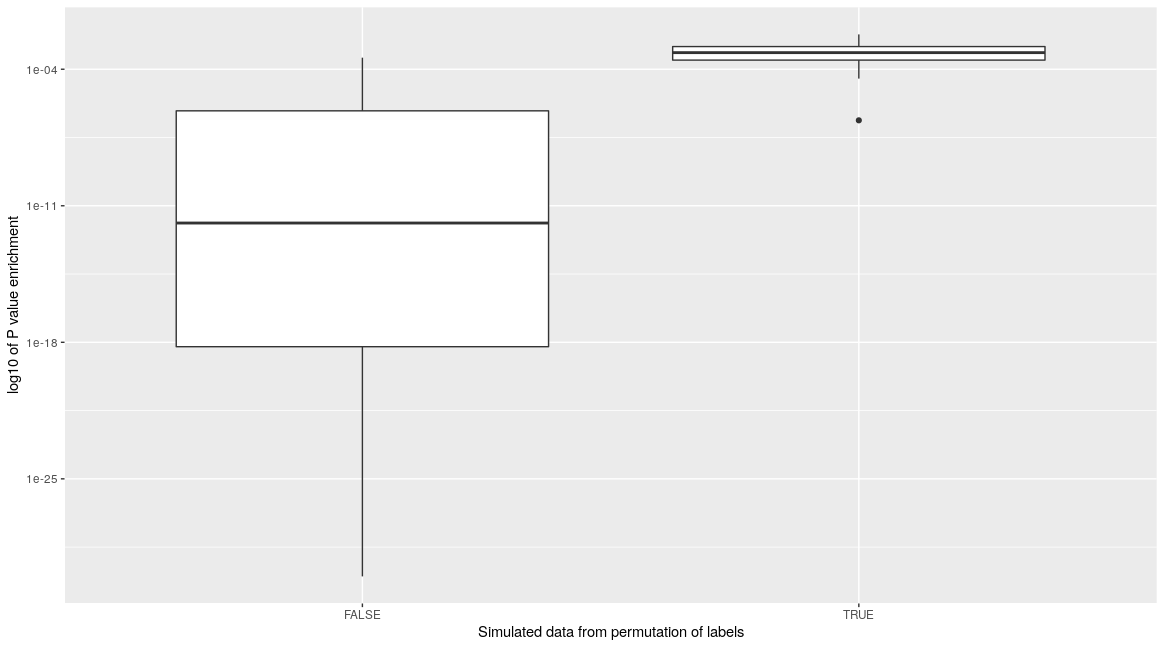
\includegraphics[width=0.9\textwidth]{images/Rplot_EnrichmentGO_permuted_labels.png}
    \caption{Enrichment p values for spectral groups Biological Process left compared with enrichment p values for groups of identical size derived from label permutation. Top p value for each group used.}
    \label{fig:topGO_permutation}
\end{figure}
% latex table generated in R 3.6.3 by xtable 1.8-4 package
% Sat Apr 11 15:28:29 2020
\begin{table}[ht]
\centering
\begin{adjustbox}{max width=\textwidth}
\begin{tabular}{lllrrrrl}
  \hline
community & GO.ID & Term & Annotated & Significant & Expected & classic & less\_than\_alpha \\ 
  \hline
1 & GO:0000226 & microtubule cytoskeleton organization & 201 & 44 & 9.64 & $3.20 \times 10^{-19}$ & TRUE \\ 
  2 & GO:0031145 & anaphase-promoting complex-dependent cat... & 34 & 30 & 1.64 & $1.00 \times 10^{-30}$ & TRUE \\ 
  3 & GO:0034762 & regulation of transmembrane transport & 203 & 10 & 2.25 & $4.60 \times 10^{-5}$ & FALSE \\ 
  4 & GO:0007031 & peroxisome organization & 36 & 13 & 0.33 & $4.30 \times 10^{-19}$ & TRUE \\ 
  5 & GO:0007186 & G protein-coupled receptor signaling pat... & 178 & 34 & 5.71 & $8.20 \times 10^{-19}$ & TRUE \\ 
  6 & GO:0097035 & regulation of membrane lipid distributio... & 9 & 5 & 0.19 & $4.50 \times 10^{-7}$ & TRUE \\ 
  7 & GO:0061640 & cytoskeleton-dependent cytokinesis & 50 & 11 & 1.84 & $1.20 \times 10^{-6}$ & TRUE \\ 
  9 & GO:0001894 & tissue homeostasis & 56 & 10 & 1.06 & $5.00 \times 10^{-8}$ & TRUE \\ 
  10 & GO:0042773 & ATP synthesis coupled electron transport & 56 & 43 & 2.57 & $1.00 \times 10^{-30}$ & TRUE \\ 
  11 & GO:0034498 & early endosome to Golgi transport & 5 & 3 & 0.08 & $3.70 \times 10^{-5}$ & FALSE \\ 
  12 & GO:0007041 & lysosomal transport & 51 & 14 & 0.50 & $3.70 \times 10^{-18}$ & TRUE \\ 
  16 & GO:0000045 & autophagosome assembly & 34 & 10 & 0.73 & $1.00 \times 10^{-9}$ & TRUE \\ 
  17 & GO:0061025 & membrane fusion & 70 & 28 & 2.92 & $9.40 \times 10^{-22}$ & TRUE \\ 
  19 & GO:0046755 & viral budding & 13 & 5 & 0.08 & $5.60 \times 10^{-9}$ & TRUE \\ 
  20 & GO:0006468 & protein phosphorylation & 535 & 65 & 23.57 & $9.70 \times 10^{-17}$ & TRUE \\ 
  22 & GO:0046328 & regulation of JNK cascade & 47 & 6 & 0.59 & $2.00 \times 10^{-5}$ & FALSE \\ 
  23 & GO:1900028 & negative regulation of ruffle assembly & 2 & 2 & 0.04 & $3.90 \times 10^{-4}$ & FALSE \\ 
  24 & GO:0006470 & protein dephosphorylation & 101 & 13 & 2.27 & $2.20 \times 10^{-7}$ & TRUE \\ 
  25 & GO:0072321 & chaperone-mediated protein transport & 7 & 3 & 0.06 & $1.60 \times 10^{-5}$ & FALSE \\ 
  26 & GO:0043408 & regulation of MAPK cascade & 172 & 33 & 6.08 & $7.40 \times 10^{-17}$ & TRUE \\ 
  28 & GO:1903361 & protein localization to basolateral plas... & 6 & 3 & 0.06 & $2.30 \times 10^{-5}$ & FALSE \\ 
  32 & GO:0051480 & regulation of cytosolic calcium ion conc... & 87 & 12 & 1.28 & $1.90 \times 10^{-9}$ & TRUE \\ 
  33 & GO:0006897 & endocytosis & 278 & 55 & 15.66 & $2.70 \times 10^{-18}$ & TRUE \\ 
  34 & GO:0007015 & actin filament organization & 172 & 60 & 10.62 & $1.00 \times 10^{-30}$ & TRUE \\ 
  43 & GO:0051276 & chromosome organization & 238 & 71 & 10.34 & $1.00 \times 10^{-30}$ & TRUE \\ 
  44 & GO:0006457 & protein folding & 102 & 25 & 3.06 & $2.60 \times 10^{-17}$ & TRUE \\ 
  45 & GO:0036503 & ERAD pathway & 27 & 13 & 0.98 & $1.30 \times 10^{-12}$ & TRUE \\ 
  46 & GO:0070202 & regulation of establishment of protein l... & 8 & 8 & 0.11 & $8.30 \times 10^{-16}$ & TRUE \\ 
  47 & GO:0035337 & fatty-acyl-CoA metabolic process & 19 & 3 & 0.15 & $3.70 \times 10^{-4}$ & FALSE \\ 
  48 & GO:0006183 & GTP biosynthetic process & 3 & 3 & 0.02 & $2.50 \times 10^{-7}$ & TRUE \\ 
  51 & GO:0006409 & tRNA export from nucleus & 12 & 9 & 0.40 & $6.70 \times 10^{-12}$ & TRUE \\ 
  53 & GO:0006413 & translational initiation & 120 & 106 & 14.17 & $1.00 \times 10^{-30}$ & TRUE \\ 
  55 & GO:0006397 & mRNA processing & 95 & 16 & 1.22 & $7.30 \times 10^{-15}$ & TRUE \\ 
  58 & GO:2001235 & positive regulation of apoptotic signali... & 53 & 6 & 0.59 & $1.90 \times 10^{-5}$ & FALSE \\ 
  62 & GO:0070125 & mitochondrial translational elongation & 32 & 15 & 0.32 & $1.00 \times 10^{-23}$ & TRUE \\ 
   \hline
\end{tabular}
\end{adjustbox}
\caption{Top term biological process Spectral clustering background PSP} 
\label{tab:Top term biological process spectral clustering background PSP}
\end{table}

% latex table generated in R 3.6.3 by xtable 1.8-4 package
% Sat Apr 11 15:39:02 2020
\begin{table}[ht]
\centering
\begin{adjustbox}{max width=\textwidth}
\begin{tabular}{lllrrrrl}
  \hline
community & GO.ID & Term & Annotated & Significant & Expected & classic & less\_than\_alpha \\ 
  \hline
1 & GO:0008017 & microtubule binding & 113 & 21 & 5.12 & $1.50 \times 10^{-8}$ & TRUE \\ 
  2 & GO:0004298 & threonine-type endopeptidase activity & 13 & 13 & 0.62 & $4.50 \times 10^{-18}$ & TRUE \\ 
  3 & GO:0008270 & zinc ion binding & 119 & 7 & 1.40 & $3.90 \times 10^{-4}$ & FALSE \\ 
  4 & GO:0031489 & myosin V binding & 14 & 4 & 0.13 & $5.90 \times 10^{-6}$ & TRUE \\ 
  5 & GO:0008066 & glutamate receptor activity & 21 & 12 & 0.66 & $1.10 \times 10^{-13}$ & TRUE \\ 
  6 & GO:0015247 & aminophospholipid transmembrane transpor... & 3 & 3 & 0.06 & $9.50 \times 10^{-6}$ & TRUE \\ 
  7 & GO:0005525 & GTP binding & 159 & 19 & 5.82 & $3.10 \times 10^{-6}$ & TRUE \\ 
  9 & GO:0005507 & copper ion binding & 12 & 4 & 0.23 & $5.30 \times 10^{-5}$ & FALSE \\ 
  10 & GO:0003954 & NADH dehydrogenase activity & 33 & 31 & 1.51 & $1.00 \times 10^{-30}$ & TRUE \\ 
  11 & GO:1990460 & leptin receptor binding & 3 & 3 & 0.05 & $3.90 \times 10^{-6}$ & TRUE \\ 
  12 & GO:0030674 & protein binding, bridging & 65 & 4 & 0.59 & $2.50 \times 10^{-3}$ & FALSE \\ 
  16 & GO:0005251 & delayed rectifier potassium channel acti... & 10 & 4 & 0.22 & $3.90 \times 10^{-5}$ & FALSE \\ 
  17 & GO:0000149 & SNARE binding & 61 & 37 & 2.64 & $1.00 \times 10^{-30}$ & TRUE \\ 
  19 & GO:0048306 & calcium-dependent protein binding & 32 & 3 & 0.19 & $8.40 \times 10^{-4}$ & FALSE \\ 
  20 & GO:0051018 & protein kinase A binding & 23 & 15 & 1.02 & $8.30 \times 10^{-16}$ & TRUE \\ 
  22 & GO:0004709 & MAP kinase kinase kinase activity & 11 & 3 & 0.14 & $2.90 \times 10^{-4}$ & FALSE \\ 
  23 & GO:0004115 & 3',5'-cyclic-AMP phosphodiesterase activ... & 4 & 2 & 0.07 & $2.00 \times 10^{-3}$ & FALSE \\ 
  24 & GO:0099181 & structural constituent of presynapse & 4 & 4 & 0.09 & $2.30 \times 10^{-7}$ & TRUE \\ 
  25 & GO:0005149 & interleukin-1 receptor binding & 2 & 2 & 0.02 & $5.50 \times 10^{-5}$ & FALSE \\ 
  26 & GO:0004708 & MAP kinase kinase activity & 9 & 8 & 0.32 & $1.60 \times 10^{-11}$ & TRUE \\ 
  28 & GO:0097016 & L27 domain binding & 4 & 4 & 0.04 & $1.30 \times 10^{-8}$ & TRUE \\ 
  32 & GO:0005261 & cation channel activity & 96 & 11 & 1.42 & $8.10 \times 10^{-8}$ & TRUE \\ 
  33 & GO:0017124 & SH3 domain binding & 55 & 29 & 3.08 & $5.60 \times 10^{-23}$ & TRUE \\ 
  34 & GO:0003779 & actin binding & 224 & 85 & 13.95 & $1.00 \times 10^{-30}$ & TRUE \\ 
  43 & GO:0003677 & DNA binding & 251 & 67 & 11.23 & $1.00 \times 10^{-30}$ & TRUE \\ 
  44 & GO:0031072 & heat shock protein binding & 52 & 25 & 1.54 & $6.30 \times 10^{-26}$ & TRUE \\ 
  45 & GO:0005342 & organic acid transmembrane transporter a... & 18 & 7 & 0.66 & $1.80 \times 10^{-6}$ & TRUE \\ 
  46 & GO:0051082 & unfolded protein binding & 56 & 9 & 0.78 & $4.00 \times 10^{-8}$ & TRUE \\ 
  47 & GO:0003996 & acyl-CoA ligase activity & 4 & 2 & 0.03 & $3.50 \times 10^{-4}$ & FALSE \\ 
  48 & GO:0061631 & ubiquitin conjugating enzyme activity & 8 & 3 & 0.05 & $1.40 \times 10^{-5}$ & TRUE \\ 
  51 & GO:0017056 & structural constituent of nuclear pore & 7 & 6 & 0.22 & $5.40 \times 10^{-9}$ & TRUE \\ 
  53 & GO:0003723 & RNA binding & 549 & 248 & 66.55 & $1.00 \times 10^{-30}$ & TRUE \\ 
  55 & GO:0003676 & nucleic acid binding & 716 & 24 & 9.09 & $5.00 \times 10^{-7}$ & TRUE \\ biological
  58 & GO:0048306 & calcium-dependent protein binding & 32 & 4 & 0.35 & $3.40 \times 10^{-4}$ & FALSE \\ 
  62 & GO:0003735 & structural constituent of ribosome & 101 & 11 & 0.95 & $6.30 \times 10^{-10}$ & TRUE \\ 
   \hline
\end{tabular}
\end{adjustbox}
\caption{Top term molecular function spectral clustering background PSP} 
\label{tab:Top term molecular function spectral clustering background PSP}
\end{table}



% latex table generated in R 3.6.3 by xtable 1.8-4 package
% Sat Apr 11 15:46:40 2020
\begin{table}[ht]
\centering
\begin{adjustbox}{max width=\textwidth}
\begin{tabular}{lllrrrrl}
  \hline
community & GO.ID & Term & Annotated & Significant & Expected & classic & less\_than\_alpha \\ 
  \hline
1 & GO:0005815 & microtubule organizing center & 238 & 57 & 11.51 & $3.20 \times 10^{-27}$ & TRUE \\ 
  2 & GO:0000502 & proteasome complex & 37 & 34 & 1.78 & $1.00 \times 10^{-30}$ & TRUE \\ 
  3 & GO:0016010 & dystrophin-associated glycoprotein compl... & 8 & 5 & 0.09 & $9.60 \times 10^{-9}$ & TRUE \\ 
  4 & GO:0005777 & peroxisome & 61 & 14 & 0.56 & $1.60 \times 10^{-17}$ & TRUE \\ 
  5 & GO:0005834 & heterotrimeric G-protein complex & 18 & 12 & 0.59 & $1.30 \times 10^{-14}$ & TRUE \\ 
  6 & GO:0016021 & integral component of membrane & 747 & 32 & 16.52 & $4.20 \times 10^{-5}$ & FALSE \\ 
   7 & GO:0005940 & septin ring & 11 & 11 & 0.40 & $1.00 \times 10^{-16}$ & TRUE \\ 
  9 & GO:0072562 & blood microparticle & 52 & 9 & 1.00 & $3.80 \times 10^{-7}$ & TRUE \\ 
  10 & GO:0070469 & respiratory chain & 54 & 42 & 2.44 & $1.00 \times 10^{-30}$ & TRUE \\ 
  11 & GO:0030905 & retromer, tubulation complex & 4 & 4 & 0.07 & $6.70 \times 10^{-8}$ & TRUE \\ 
  12 & GO:0030897 & HOPS complex & 7 & 7 & 0.07 & $5.30 \times 10^{-15}$ & TRUE \\ 
  16 & GO:0000421 & autophagosome membrane & 11 & 6 & 0.23 & $3.20 \times 10^{-8}$ & TRUE \\ 
  17 & GO:0031201 & SNARE complex & 28 & 25 & 1.18 & $1.00 \times 10^{-30}$ & TRUE \\ 
  19 & GO:0000813 & ESCRT I complex & 3 & 3 & 0.02 & $1.50 \times 10^{-7}$ & TRUE \\ 
  20 & GO:0005886 & plasma membrane & 1276 & 94 & 56.07 & $1.10 \times 10^{-10}$ & TRUE \\ 
  22 & GO:0008043 & intracellular ferritin complex & 2 & 2 & 0.02 & $1.50 \times 10^{-4}$ & FALSE \\ 
  23 & GO:0034045 & phagophore assembly site membrane & 8 & 2 & 0.16 & $9.70 \times 10^{-3}$ & FALSE \\ 
  24 & GO:0000159 & protein phosphatase type 2A complex & 10 & 7 & 0.22 & $2.20 \times 10^{-10}$ & TRUE \\ 
  25 & GO:0042719 & mitochondrial intermembrane space protei... & 3 & 2 & 0.02 & $1.70 \times 10^{-4}$ & FALSE \\ 
  26 & GO:0071944 & cell periphery & 1338 & 78 & 47.35 & $7.70 \times 10^{-9}$ & TRUE \\ 
  28 & GO:0005923 & bicellular tight junction & 44 & 11 & 0.47 & $2.20 \times 10^{-13}$ & TRUE \\ 
  32 & GO:0034703 & cation channel complex & 96 & 11 & 1.47 & $1.20 \times 10^{-7}$ & TRUE \\ 
  33 & GO:0071944 & cell periphery & 1338 & 121 & 74.18 & $1.10 \times 10^{-12}$ & TRUE \\ 
  34 & GO:0015629 & actin cytoskeleton & 260 & 92 & 16.25 & $1.00 \times 10^{-30}$ & TRUE \\ 
  43 & GO:0031981 & nuclear lumen & 856 & 111 & 36.86 & $1.00 \times 10^{-30}$ & TRUE \\ 
  44 & GO:0101031 & chaperone complex & 20 & 8 & 0.59 & $4.10 \times 10^{-8}$ & TRUE \\ 
  45 & GO:0044432 & endoplasmic reticulum part & 292 & 32 & 10.68 & $5.40 \times 10^{-9}$ & TRUE \\ 
  46 & GO:0005832 & chaperonin-containing T-complex & 9 & 9 & 0.13 & $1.00 \times 10^{-17}$ & TRUE \\ 
  47 & GO:0005778 & peroxisomal membrane & 33 & 5 & 0.25 & $3.60 \times 10^{-6}$ & TRUE \\ 
  48 & GO:0031371 & ubiquitin conjugating enzyme complex & 5 & 3 & 0.03 & $2.00 \times 10^{-6}$ & TRUE \\ 
  51 & GO:0005643 & nuclear pore & 25 & 12 & 0.81 & $2.70 \times 10^{-12}$ & TRUE \\ 
  53 & GO:1990904 & ribonucleoprotein complex & 293 & 184 & 34.65 & $1.00 \times 10^{-30}$ & TRUE \\ 
  55 & GO:0016607 & nuclear speck & 83 & 15 & 1.08 & $2.40 \times 10^{-14}$ & TRUE \\ 
  58 & GO:0030127 & COPII vesicle coat & 9 & 4 & 0.10 & $1.50 \times 10^{-6}$ & TRUE \\ 
  62 & GO:0000315 & organellar large ribosomal subunit & 15 & 14 & 0.15 & $7.00 \times 10^{-29}$ & TRUE \\ 
   \hline
\end{tabular}
\end{adjustbox}
\caption{Top term CC background spectral clustering PSP} 
\label{tab:Top term CC background spectral clustering PSP}
\end{table}

\begin{table}[]
    \centering
    \begin{tabular}{lllll}
    \toprule
          & Degree & Eigenvector centrality & Closeness & Betweenness \\
         \midrule
    Degree  & 1  & 0.92  & 0.66 & 0.85\\
    Eigenvector centrality & 0.92 & 1 & 0.63 & 0.72  \\
    Closeness & 0.66 & 0.63 & 1 & 0.44  \\
    Betweenness& 0.85 & 0.72 & 0.44 & 1 \\
    \bottomrule
    \end{tabular}
    \caption{Correlation of centrality measures for 58 sociometric network datasets from Valente et al \cite{valente2008correlated}. Pearson correlation coefficient. Values are for symmetrised closeness and betweenness centrality. Eigenvector centrality is necessarily symmetrised. Range of average network size 45-83. Some studies had maximal nominations for degree}
    \label{tab:Correlation of centrality valente et al}
\end{table}

\subsection{GO Louvain}
% latex table generated in R 3.6.3 by xtable 1.8-4 package
% Sat Apr 18 17:57:38 2020
\begin{table}[ht]
\centering
\begin{adjustbox}{max width=\textwidth}
\begin{tabular}{lllrrrrl}
  \hline
community & GO.ID & Term & Annotated & Significant & Expected & classic & less\_than\_alpha \\ 
  \hline
1 & GO:0006625 & protein targeting to peroxisome & 29 & 16 & 2 & $5.70 \times 10^{-13}$ & TRUE \\ 
  2 & GO:0042773 & ATP synthesis coupled electron transport & 56 & 45 & 6 & $1.00 \times 10^{-30}$ & TRUE \\ 
  3 & GO:0016071 & mRNA metabolic process & 254 & 165 & 39 & $1.00 \times 10^{-30}$ & TRUE \\ 
  4 & GO:0051276 & chromosome organization & 238 & 99 & 18 & $1.00 \times 10^{-30}$ & TRUE \\ 
  5 & GO:0070202 & regulation of establishment of protein l... & 8 & 8 & 0 & $1.00 \times 10^{-12}$ & TRUE \\ 
  6 & GO:0031145 & anaphase-promoting complex-dependent cat... & 34 & 30 & 2 & $1.00 \times 10^{-30}$ & TRUE \\ 
  7 & GO:0007215 & glutamate receptor signaling pathway & 64 & 25 & 3 & $1.30 \times 10^{-18}$ & TRUE \\ 
  8 & GO:0006468 & protein phosphorylation & 535 & 196 & 84 & $1.00 \times 10^{-30}$ & TRUE \\ 
  9 & GO:0030029 & actin filament-based process & 333 & 141 & 43 & $1.00 \times 10^{-30}$ & TRUE \\ 
  10 & GO:0016236 & macroautophagy & 125 & 19 & 2 & $5.60 \times 10^{-14}$ & TRUE \\ 
  11 & GO:0097711 & ciliary basal body-plasma membrane docki... & 48 & 27 & 5 & $4.70 \times 10^{-16}$ & TRUE \\ 
  12 & GO:0015696 & ammonium transport & 25 & 4 & 0 & $1.30 \times 10^{-5}$ & FALSE \\ 
  13 & GO:0001732 & formation of cytoplasmic translation ini... & 11 & 10 & 0 & $3.30 \times 10^{-16}$ & TRUE \\ 
  14 & GO:0061025 & membrane fusion & 70 & 30 & 4 & $1.30 \times 10^{-21}$ & TRUE \\ 
   \hline
\end{tabular}
\end{adjustbox}
\caption{Top term  lourvain BP background PSP} 
\label{tab:Top term  lourvain BP background PSP}
\end{table}

% latex table generated in R 3.6.3 by xtable 1.8-4 package
% Sat Apr 18 17:58:35 2020
\begin{table}[ht]
\centering
\begin{tabular}{lr}
  \hline
quantile & value of p \\ 
  \hline
0\% & $1.000 \times 10^{-30}$ \\ 
  25\% & $1.000 \times 10^{-30}$ \\ 
  50\% & $6.506 \times 10^{-19}$ \\ 
  75\% & $4.212 \times 10^{-14}$ \\ 
  100\% & $1.300 \times 10^{-5}$ \\ 
   \hline
\end{tabular}
\caption{P values for different quantiles for lourvain clusteringBP} 
\label{tabP values for different quantiles for lourvain clusteringBP}
\end{table}

\subsubsection{Molecular function}
% latex table generated in R 3.6.3 by xtable 1.8-4 package
% Sat Apr 18 17:59:47 2020
\begin{table}[ht]
\centering
\begin{adjustbox}{max width=\textwidth}
\begin{tabular}{lllrrrrl}
  \hline
community & GO.ID & Term & Annotated & Significant & Expected & classic & less\_than\_alpha \\ 
  \hline
1 & GO:0034987 & immunoglobulin receptor binding & 8 & 6 & 0 & $1.10 \times 10^{-6}$ & TRUE \\ 
  2 & GO:0003954 & NADH dehydrogenase activity & 33 & 30 & 3 & $1.60 \times 10^{-27}$ & TRUE \\ 
  3 & GO:0003723 & RNA binding & 549 & 298 & 86 & $1.00 \times 10^{-30}$ & TRUE \\ 
  4 & GO:0003677 & DNA binding & 251 & 86 & 20 & $1.00 \times 10^{-30}$ & TRUE \\ 
  5 & GO:0051721 & protein phosphatase 2A binding & 9 & 6 & 0 & $9.10 \times 10^{-8}$ & TRUE \\ 
  6 & GO:0004298 & threonine-type endopeptidase activity & 13 & 13 & 1 & $4.90 \times 10^{-18}$ & TRUE \\ 
  7 & GO:0038023 & signaling receptor activity & 128 & 32 & 6 & $5.40 \times 10^{-17}$ & TRUE \\ 
  8 & GO:0004672 & protein kinase activity & 195 & 103 & 30 & $1.00 \times 10^{-30}$ & TRUE \\ 
  9 & GO:0003779 & actin binding & 224 & 107 & 29 & $1.00 \times 10^{-30}$ & TRUE \\ 
  10 & GO:0017137 & Rab GTPase binding & 63 & 10 & 1 & $6.50 \times 10^{-8}$ & TRUE \\ 
  11 & GO:0008017 & microtubule binding & 113 & 30 & 11 & $1.40 \times 10^{-7}$ & TRUE \\ 
  12 & GO:0005544 & calcium-dependent phospholipid binding & 27 & 4 & 0 & $1.90 \times 10^{-5}$ & TRUE \\ 
  13 & GO:0003743 & translation initiation factor activity & 27 & 14 & 1 & $5.20 \times 10^{-17}$ & TRUE \\ 
  14 & GO:0000149 & SNARE binding & 61 & 33 & 3 & $1.70 \times 10^{-28}$ & TRUE \\ 
   \hline
\end{tabular}
\end{adjustbox}
\caption{Top term  lourvain MF background PSP} 
\label{tab:Top term  lourvain MF background PSP}
\end{table}


% latex table generated in R 3.6.3 by xtable 1.8-4 package
% Sat Apr 18 18:00:33 2020
\begin{table}[ht]
\centering

\begin{tabular}{lr}
  \hline
quantile & value of p \\ 
  \hline
0\% & $1.000 \times 10^{-30}$ \\ 
  25\% & $4.325 \times 10^{-29}$ \\ 
  50\% & $2.845 \times 10^{-17}$ \\ 
  75\% & $8.450 \times 10^{-8}$ \\ 
  100\% & $1.900 \times 10^{-5}$ \\ 
   \hline
\end{tabular}
\caption{P values for different quantiles for lourvain clusteringMF} 
\label{tabP values for different quantiles for lourvain clusteringMF}
\end{table}

\subsubsection{Cellular compartment}



\subsection{topgo Infomap}

% latex table generated in R 3.6.3 by xtable 1.8-4 package
% Sat Apr 18 18:17:43 2020
% latex table generated in R 3.6.3 by xtable 1.8-4 package
% Sat Apr 18 18:35:49 2020
\begin{table}[ht]
\centering
\begin{adjustbox}{max width=\textwidth}
\begin{tabular}{lllrrrrl}
  \hline
community & GO.ID & Term & Annotated & Significant & Expected & classic & less\_than\_alpha \\ 
  \hline
1 & GO:0090304 & nucleic acid metabolic process & 801 & 505 & 287 & $1.00 \times 10^{-30}$ & TRUE \\ 
  2 & GO:0030029 & actin filament-based process & 333 & 71 & 12 & $1.00 \times 10^{-30}$ & TRUE \\ 
  3 & GO:0006897 & endocytosis & 278 & 41 & 10 & $2.60 \times 10^{-17}$ & TRUE \\ 
  4 & GO:0000226 & microtubule cytoskeleton organization & 201 & 28 & 5 & $2.90 \times 10^{-16}$ & TRUE \\ 
  5 & GO:0070202 & regulation of establishment of protein l... & 8 & 8 & 0 & $1.20 \times 10^{-15}$ & TRUE \\ 
  6 & GO:0006521 & regulation of cellular amino acid metabo... & 33 & 28 & 0 & $1.00 \times 10^{-30}$ & TRUE \\ 
  7 & GO:0070268 & cornification & 41 & 12 & 1 & $9.90 \times 10^{-13}$ & TRUE \\ 
  8 & GO:0045821 & positive regulation of glycolytic proces... & 5 & 2 & 0 & $3.30 \times 10^{-3}$ & FALSE \\ 
  9 & GO:0090383 & phagosome acidification & 15 & 15 & 0 & $4.30 \times 10^{-29}$ & TRUE \\ 
  10 & GO:0030036 & actin cytoskeleton organization & 284 & 28 & 4 & $5.00 \times 10^{-18}$ & TRUE \\ 
  11 & GO:0099537 & trans-synaptic signaling & 316 & 28 & 5 & $1.80 \times 10^{-16}$ & TRUE \\ 
  12 & GO:0010257 & NADH dehydrogenase complex assembly & 34 & 31 & 0 & $1.00 \times 10^{-30}$ & TRUE \\ 
  13 & GO:0060384 & innervation & 10 & 2 & 0 & $5.10 \times 10^{-3}$ & FALSE \\ 
  14 & GO:0061025 & membrane fusion & 70 & 25 & 1 & $1.00 \times 10^{-30}$ & TRUE \\ 
  15 & GO:0000045 & autophagosome assembly & 34 & 10 & 0 & $2.20 \times 10^{-13}$ & TRUE \\ 
  16 & GO:0007186 & G protein-coupled receptor signaling pat... & 178 & 25 & 2 & $2.70 \times 10^{-26}$ & TRUE \\ 
  17 & GO:0034199 & activation of protein kinase A activity & 10 & 6 & 0 & $1.10 \times 10^{-11}$ & TRUE \\ 
  18 & GO:0010921 & regulation of phosphatase activity & 56 & 10 & 1 & $2.60 \times 10^{-11}$ & TRUE \\ 
  19 & GO:0005513 & detection of calcium ion & 5 & 3 & 0 & $4.20 \times 10^{-6}$ & TRUE \\ 
  20 & GO:0070125 & mitochondrial translational elongation & 32 & 16 & 0 & $6.80 \times 10^{-28}$ & TRUE \\ 
  21 & GO:0031175 & neuron projection development & 404 & 10 & 3 & $1.60 \times 10^{-4}$ & FALSE \\ 
  22 & GO:0006893 & Golgi to plasma membrane transport & 33 & 5 & 0 & $3.90 \times 10^{-6}$ & TRUE \\ 
  23 & GO:0002495 & antigen processing and presentation of p... & 53 & 10 & 0 & $6.90 \times 10^{-14}$ & TRUE \\ 
  24 & GO:0007215 & glutamate receptor signaling pathway & 64 & 13 & 0 & $5.80 \times 10^{-18}$ & TRUE \\ 
  25 & GO:0051403 & stress-activated MAPK cascade & 80 & 12 & 0 & $8.70 \times 10^{-17}$ & TRUE \\ 
  27 & GO:0006869 & lipid transport & 65 & 5 & 0 & $1.20 \times 10^{-5}$ & FALSE \\ 
  28 & GO:0002221 & pattern recognition receptor signaling p... & 40 & 5 & 0 & $1.10 \times 10^{-6}$ & TRUE \\ 
  29 & GO:0006816 & calcium ion transport & 144 & 14 & 1 & $1.10 \times 10^{-16}$ & TRUE \\ 
  30 & GO:0006637 & acyl-CoA metabolic process & 40 & 10 & 0 & $3.30 \times 10^{-16}$ & TRUE \\ 
  31 & GO:1902531 & regulation of intracellular signal trans... & 468 & 7 & 2 & $2.40 \times 10^{-3}$ & FALSE \\ 
  32 & GO:0061640 & cytoskeleton-dependent cytokinesis & 50 & 11 & 0 & $3.50 \times 10^{-18}$ & TRUE \\ 
  34 & GO:0006625 & protein targeting to peroxisome & 29 & 14 & 0 & $9.80 \times 10^{-28}$ & TRUE \\ 
  35 & GO:1904340 & positive regulation of dopaminergic neur... & 2 & 2 & 0 & $1.60 \times 10^{-5}$ & FALSE \\ 
  36 & GO:0006957 & complement activation, alternative pathw... & 2 & 2 & 0 & $2.70 \times 10^{-5}$ & FALSE \\ 
  40 & GO:0006936 & muscle contraction & 124 & 7 & 1 & $2.30 \times 10^{-7}$ & TRUE \\ 
  46 & GO:0034204 & lipid translocation & 6 & 4 & 0 & $3.90 \times 10^{-9}$ & TRUE \\ 
  52 & GO:0098659 & inorganic cation import across plasma me... & 25 & 4 & 0 & $2.30 \times 10^{-6}$ & TRUE \\ 
   \hline
\end{tabular}
\end{adjustbox}
\caption{Top term  infomap BP background PSP} 
\label{tab:Top term  infomap BP background PSP}
\end{table}


% latex table generated in R 3.6.3 by xtable 1.8-4 package
% Sat Apr 18 18:17:43 2020
\begin{table}[ht]
\centering

\begin{tabular}{lr}
  \hline
quantile & value of p \\ 
  \hline
0\% & $1.000 \times 10^{-30}$ \\ 
  25\% & $3.500 \times 10^{-18}$ \\ 
  50\% & $1.200 \times 10^{-15}$ \\ 
  75\% & $2.300 \times 10^{-6}$ \\ 
  100\% & $5.100 \times 10^{-3}$ \\ 
   \hline
\end{tabular}
\caption{P values for different quantiles for infomap clusteringBP} 
\label{tabP values for different quantiles for infomap clusteringBP}
\end{table}

\subsubsection{MF topgo infomap}
% latex table generated in R 3.6.3 by xtable 1.8-4 package
% Sat Apr 18 20:16:53 2020
\begin{table}[ht]
\centering
\begin{adjustbox}{max width=\textwidth}
\begin{tabular}{lllrrrrl}
  \hline
community & GO.ID & Term & Annotated & Significant & Expected & classic & less\_than\_alpha \\ 
  \hline
1 & GO:1990904 & ribonucleoprotein complex & 293 & 230 & 105 & $1.00 \times 10^{-30}$ & TRUE \\ 
  2 & GO:0015629 & actin cytoskeleton & 260 & 79 & 10 & $1.00 \times 10^{-30}$ & TRUE \\ 
  3 & GO:0071944 & cell periphery & 1338 & 91 & 46 & $9.40 \times 10^{-18}$ & TRUE \\ 
  4 & GO:0015630 & microtubule cytoskeleton & 407 & 48 & 9 & $1.40 \times 10^{-25}$ & TRUE \\ 
  5 & GO:0005832 & chaperonin-containing T-complex & 9 & 9 & 0 & $1.50 \times 10^{-17}$ & TRUE \\ 
  6 & GO:0000502 & proteasome complex & 37 & 31 & 0 & $1.00 \times 10^{-30}$ & TRUE \\ 
  7 & GO:0005882 & intermediate filament & 64 & 13 & 1 & $4.40 \times 10^{-11}$ & TRUE \\ 
  8 & GO:0097427 & microtubule bundle & 5 & 2 & 0 & $3.40 \times 10^{-3}$ & FALSE \\ 
  9 & GO:0033176 & proton-transporting V-type ATPase comple... & 13 & 13 & 0 & $2.10 \times 10^{-25}$ & TRUE \\ 
  10 & GO:0031209 & SCAR complex & 8 & 7 & 0 & $5.70 \times 10^{-13}$ & TRUE \\ 
  11 & GO:0097060 & synaptic membrane & 219 & 29 & 3 & $2.30 \times 10^{-22}$ & TRUE \\ 
  12 & GO:0005747 & mitochondrial respiratory chain complex ... & 34 & 31 & 0 & $1.00 \times 10^{-30}$ & TRUE \\ 
  13 & GO:0031232 & extrinsic component of external side of ... & 4 & 1 & 0 & $4.60 \times 10^{-2}$ & FALSE \\ 
  14 & GO:0031201 & SNARE complex & 28 & 25 & 0 & $1.00 \times 10^{-30}$ & TRUE \\ 
  15 & GO:0000421 & autophagosome membrane & 11 & 7 & 0 & $1.30 \times 10^{-12}$ & TRUE \\ 
  16 & GO:0005834 & heterotrimeric G-protein complex & 18 & 11 & 0 & $5.20 \times 10^{-19}$ & TRUE \\ 
  17 & GO:0005952 & cAMP-dependent protein kinase complex & 8 & 7 & 0 & $1.90 \times 10^{-15}$ & TRUE \\ 
  18 & GO:0000164 & protein phosphatase type 1 complex & 5 & 3 & 0 & $6.80 \times 10^{-6}$ & TRUE \\ 
  19 & GO:0034704 & calcium channel complex & 33 & 5 & 0 & $4.40 \times 10^{-6}$ & TRUE \\ 
  20 & GO:0000315 & organellar large ribosomal subunit & 15 & 15 & 0 & $1.00 \times 10^{-30}$ & TRUE \\ 
  21 & GO:0048787 & presynaptic active zone membrane & 18 & 2 & 0 & $5.80 \times 10^{-3}$ & FALSE \\ 
  22 & GO:0099023 & tethering complex & 33 & 5 & 0 & $3.60 \times 10^{-6}$ & TRUE \\ 
  23 & GO:0005875 & microtubule associated complex & 57 & 13 & 0 & $1.40 \times 10^{-19}$ & TRUE \\ 
  24 & GO:0045211 & postsynaptic membrane & 160 & 16 & 1 & $1.70 \times 10^{-17}$ & TRUE \\ 
  25 & GO:0097458 & neuron part & 812 & 10 & 4 & $2.10 \times 10^{-3}$ & FALSE \\ 
  27 & GO:0030905 & retromer, tubulation complex & 4 & 4 & 0 & $4.30 \times 10^{-10}$ & TRUE \\ 
  28 & GO:0005741 & mitochondrial outer membrane & 86 & 5 & 0 & $4.50 \times 10^{-5}$ & FALSE \\ 
  29 & GO:0016529 & sarcoplasmic reticulum & 31 & 8 & 0 & $7.60 \times 10^{-13}$ & TRUE \\ 
  30 & GO:0045254 & pyruvate dehydrogenase complex & 6 & 6 & 0 & $5.90 \times 10^{-15}$ & TRUE \\ 
  31 & GO:0038038 & G protein-coupled receptor homodimeric c... & 1 & 1 & 0 & $4.40 \times 10^{-3}$ & FALSE \\ 
  32 & GO:0005940 & septin ring & 11 & 11 & 0 & $8.10 \times 10^{-29}$ & TRUE \\ 
  34 & GO:0005777 & peroxisome & 61 & 17 & 0 & $3.40 \times 10^{-30}$ & TRUE \\ 
  35 & GO:0030285 & integral component of synaptic vesicle m... & 19 & 2 & 0 & $2.60 \times 10^{-3}$ & FALSE \\ 
  36 & GO:0072562 & blood microparticle & 52 & 7 & 0 & $3.70 \times 10^{-9}$ & TRUE \\ 
  40 & GO:0016010 & dystrophin-associated glycoprotein compl... & 8 & 5 & 0 & $4.50 \times 10^{-11}$ & TRUE \\ 
  46 & GO:0016021 & integral component of membrane & 747 & 12 & 3 & $2.80 \times 10^{-6}$ & TRUE \\ 
  52 & GO:0016021 & integral component of membrane & 747 & 13 & 3 & $1.80 \times 10^{-7}$ & TRUE \\ 
   \hline
\end{tabular}
\end{adjustbox}


\caption{Top term  infomap CC background PSP} 
\label{tab:Top term  infomap CC background PSP}
\end{table}
% latex table generated in R 3.6.3 by xtable 1.8-4 package
% Sat Apr 18 20:16:53 2020
\begin{table}[ht]
\centering
\begin{tabular}{lr}
  \hline
quantile & value of p \\ 
  \hline
0\% & $1.000 \times 10^{-30}$ \\ 
  25\% & $2.100 \times 10^{-25}$ \\ 
  50\% & $5.700 \times 10^{-13}$ \\ 
  75\% & $3.600 \times 10^{-6}$ \\ 
  100\% & $4.600 \times 10^{-2}$ \\ 
   \hline
\end{tabular}
\caption{P values for different quantiles for infomap clusteringCC} 
\label{tabP values for different quantiles for infomap clusteringCC}
\end{table}


% latex table generated in R 3.6.3 by xtable 1.8-4 package
% Sat Apr 18 18:37:55 2020
\begin{table}[ht]
\centering
\begin{adjustbox}{max width=\textwidth}
\begin{tabular}{lllrrrrl}
  \hline
community & GO.ID & Term & Annotated & Significant & Expected & classic & less\_than\_alpha \\ 
  \hline
1 & GO:0003676 & nucleic acid binding & 716 & 506 & 260 & $1.00 \times 10^{-30}$ & TRUE \\ 
  2 & GO:0003779 & actin binding & 224 & 76 & 9 & $1.00 \times 10^{-30}$ & TRUE \\ 
  3 & GO:0017124 & SH3 domain binding & 55 & 22 & 2 & $2.90 \times 10^{-19}$ & TRUE \\ 
  4 & GO:0008017 & microtubule binding & 113 & 11 & 2 & $1.80 \times 10^{-5}$ & TRUE \\ 
  5 & GO:0019888 & protein phosphatase regulator activity & 24 & 7 & 0 & $2.90 \times 10^{-8}$ & TRUE \\ 
  6 & GO:0004298 & threonine-type endopeptidase activity & 13 & 12 & 0 & $2.90 \times 10^{-23}$ & TRUE \\ 
  7 & GO:0005200 & structural constituent of cytoskeleton & 74 & 6 & 1 & $2.30 \times 10^{-3}$ & FALSE \\ 
  8 & GO:0016836 & hydro-lyase activity & 22 & 5 & 0 & $3.20 \times 10^{-5}$ & FALSE \\ 
  9 & GO:0036442 & proton-exporting ATPase activity & 19 & 14 & 0 & $4.90 \times 10^{-23}$ & TRUE \\ 
  10 & GO:0017048 & Rho GTPase binding & 79 & 16 & 1 & $2.90 \times 10^{-15}$ & TRUE \\ 
  11 & GO:0030165 & PDZ domain binding & 41 & 10 & 1 & $1.90 \times 10^{-10}$ & TRUE \\ 
  12 & GO:0003954 & NADH dehydrogenase activity & 33 & 30 & 0 & $1.00 \times 10^{-30}$ & TRUE \\ 
  13 & GO:0004860 & protein kinase inhibitor activity & 20 & 3 & 0 & $1.40 \times 10^{-3}$ & FALSE \\ 
  14 & GO:0000149 & SNARE binding & 61 & 29 & 1 & $1.00 \times 10^{-30}$ & TRUE \\ 
  15 & GO:0017137 & Rab GTPase binding & 63 & 9 & 1 & $6.60 \times 10^{-9}$ & TRUE \\ 
  16 & GO:0003924 & GTPase activity & 153 & 21 & 1 & $2.00 \times 10^{-21}$ & TRUE \\ 
  17 & GO:0051018 & protein kinase A binding & 23 & 11 & 0 & $3.60 \times 10^{-20}$ & TRUE \\ 
  18 & GO:0019888 & protein phosphatase regulator activity & 24 & 7 & 0 & $5.70 \times 10^{-10}$ & TRUE \\ 
  19 & GO:0005516 & calmodulin binding & 103 & 8 & 1 & $3.30 \times 10^{-7}$ & TRUE \\ 
  20 & GO:0003735 & structural constituent of ribosome & 101 & 12 & 1 & $2.30 \times 10^{-12}$ & TRUE \\ 
  21 & GO:0031005 & filamin binding & 5 & 3 & 0 & $2.90 \times 10^{-6}$ & TRUE \\ 
  22 & GO:0004823 & leucine-tRNA ligase activity & 1 & 1 & 0 & $7.60 \times 10^{-3}$ & FALSE \\ 
  23 & GO:0003774 & motor activity & 67 & 6 & 0 & $1.70 \times 10^{-6}$ & TRUE \\ 
  24 & GO:0008066 & glutamate receptor activity & 21 & 12 & 0 & $1.00 \times 10^{-23}$ & TRUE \\ 
  25 & GO:0004712 & protein serine/threonine/tyrosine kinase... & 15 & 5 & 0 & $5.50 \times 10^{-9}$ & TRUE \\ 
  27 & GO:1990460 & leptin receptor binding & 3 & 3 & 0 & $1.40 \times 10^{-7}$ & TRUE \\ 
  28 & GO:0019900 & kinase binding & 250 & 6 & 1 & $1.10 \times 10^{-3}$ & FALSE \\ 
  29 & GO:0005262 & calcium channel activity & 47 & 9 & 0 & $4.70 \times 10^{-13}$ & TRUE \\ 
  30 & GO:0016903 & oxidoreductase activity, acting on the a... & 21 & 8 & 0 & $1.40 \times 10^{-14}$ & TRUE \\ 
  31 & GO:0017048 & Rho GTPase binding & 79 & 3 & 0 & $3.90 \times 10^{-3}$ & FALSE \\ 
  32 & GO:0003924 & GTPase activity & 153 & 11 & 1 & $1.70 \times 10^{-12}$ & TRUE \\ 
  34 & GO:0071949 & FAD binding & 9 & 3 & 0 & $1.10 \times 10^{-5}$ & TRUE \\ 
  35 & GO:0050321 & tau-protein kinase activity & 17 & 2 & 0 & $1.90 \times 10^{-3}$ & FALSE \\ 
  36 & GO:0019825 & oxygen binding & 4 & 2 & 0 & $1.70 \times 10^{-4}$ & FALSE \\ 
  40 & GO:0008270 & zinc ion binding & 119 & 6 & 1 & $7.30 \times 10^{-6}$ & TRUE \\ 
  46 & GO:0015247 & aminophospholipid transmembrane transpor... & 3 & 3 & 0 & $6.00 \times 10^{-8}$ & TRUE \\ 
  52 & GO:0022857 & transmembrane transporter activity & 250 & 8 & 1 & $1.90 \times 10^{-6}$ & TRUE \\ 
   \hline
\end{tabular}
\end{adjustbox}
\caption{Top term  infomap MF background PSP} 
\label{tab:Top term  infomap MF background PSP}
\end{table}
% latex table generated in R 3.6.3 by xtable 1.8-4 package
% Sat Apr 18 18:37:55 2020
\begin{table}[ht]
\centering
\begin{tabular}{lr}
  \hline
quantile & value of p \\ 
  \hline
0\% & $1.000 \times 10^{-30}$ \\ 
  25\% & $2.900 \times 10^{-19}$ \\ 
  50\% & $6.600 \times 10^{-9}$ \\ 
  75\% & $1.100 \times 10^{-5}$ \\ 
  100\% & $7.600 \times 10^{-3}$ \\ 
   \hline
\end{tabular}
\caption{P values for different quantiles for infomap clusteringMF} 
\label{tabP values for different quantiles for infomap clusteringMF}
\end{table}

\subsection{lec}

% latex table generated in R 3.6.3 by xtable 1.8-4 package
% Sat Apr 18 20:20:18 2020
\begin{table}[ht]
\centering
\begin{adjustbox}{max width=\textwidth}
\begin{tabular}{lllrrrrl}
  \hline
community & GO.ID & Term & Annotated & Significant & Expected & classic & less\_than\_alpha \\ 
  \hline
1 & GO:0030036 & actin cytoskeleton organization & 284 & 188 & 94 & $1.00 \times 10^{-30}$ & TRUE \\ 
  2 & GO:0034641 & cellular nitrogen compound metabolic pro... & 1208 & 621 & 394 & $1.00 \times 10^{-30}$ & TRUE \\ 
  3 & GO:0010257 & NADH dehydrogenase complex assembly & 34 & 33 & 12 & $8.10 \times 10^{-15}$ & TRUE \\ 
   \hline
\end{tabular}
\end{adjustbox}
\caption{Top term  lec BP background PSP} 
\label{tab:Top term  lec BP background PSP}
\end{table}

% latex table generated in R 3.6.3 by xtable 1.8-4 package
% Sat Apr 18 20:20:18 2020
\begin{table}[ht]
\centering
\begin{tabular}{lr}
  \hline
quantile & value of p \\ 
  \hline
0\% & $1.000 \times 10^{-30}$ \\ 
  25\% & $1.000 \times 10^{-30}$ \\ 
  50\% & $1.000 \times 10^{-30}$ \\ 
  75\% & $4.050 \times 10^{-15}$ \\ 
  100\% & $8.100 \times 10^{-15}$ \\ 
   \hline
\end{tabular}
\caption{P values for different quantiles for lec clusteringBP} 
\label{tabP values for different quantiles for lec clusteringBP}
\end{table}

\subsection{Lec size off}

greater than 5

\section{Ontology of centrality measures}
code for eigenvector at \url{source('~/RProjects/group_sizes/R/plotting/modified_exampleGoObject_summary_PSP_centrality_eigenvector.R')}
\subsection{Betweenness}
% latex table generated in R 3.6.3 by xtable 1.8-4 package
% Sat May 16 16:08:21 2020
\begin{table}[ht]
\centering
\begin{tabular}{llrrrr}
  \hline
GO.ID & Term & Annotated & Significant & Expected & classic \\ 
  \hline
GO:0051246 & regulation of protein metabolic process & 677 & 93 & 34.9 & $5.70 \times 10^{-24}$ \\ 
  GO:0007049 & cell cycle & 458 & 74 & 23.6 & $2.10 \times 10^{-22}$ \\ 
  GO:0051171 & regulation of nitrogen compound metaboli... & 1070 & 113 & 55.1 & $1.50 \times 10^{-20}$ \\ 
  GO:0032268 & regulation of cellular protein metabolic... & 623 & 84 & 32.1 & $2.00 \times 10^{-20}$ \\ 
  GO:0080090 & regulation of primary metabolic process & 1111 & 115 & 57.3 & $2.50 \times 10^{-20}$ \\ 
  GO:0009057 & macromolecule catabolic process & 431 & 68 & 22.2 & $1.10 \times 10^{-19}$ \\ 
  GO:0060255 & regulation of macromolecule metabolic pr... & 1167 & 117 & 60.1 & $1.30 \times 10^{-19}$ \\ 
  GO:0006950 & response to stress & 872 & 99 & 45.0 & $3.10 \times 10^{-19}$ \\ 
  GO:0009894 & regulation of catabolic process & 326 & 58 & 16.8 & $4.20 \times 10^{-19}$ \\ 
  GO:0051704 & multi-organism process & 597 & 80 & 30.8 & $4.90 \times 10^{-19}$ \\ 
  GO:0031323 & regulation of cellular metabolic process & 1167 & 115 & 60.1 & $2.20 \times 10^{-18}$ \\ 
  GO:0031399 & regulation of protein modification proce... & 442 & 67 & 22.8 & $2.30 \times 10^{-18}$ \\ 
  GO:0043412 & macromolecule modification & 911 & 100 & 47.0 & $2.40 \times 10^{-18}$ \\ 
  GO:0006464 & cellular protein modification process & 899 & 99 & 46.3 & $3.40 \times 10^{-18}$ \\ 
  GO:0036211 & protein modification process & 899 & 99 & 46.3 & $3.40 \times 10^{-18}$ \\ 
  GO:0051247 & positive regulation of protein metabolic... & 409 & 64 & 21.1 & $3.50 \times 10^{-18}$ \\ 
  GO:0010604 & positive regulation of macromolecule met... & 658 & 83 & 33.9 & $3.80 \times 10^{-18}$ \\ 
  GO:0009893 & positive regulation of metabolic process & 733 & 88 & 37.8 & $4.80 \times 10^{-18}$ \\ 
  GO:0048523 & negative regulation of cellular process & 1062 & 108 & 54.7 & $9.80 \times 10^{-18}$ \\ 
  GO:0030163 & protein catabolic process & 263 & 50 & 13.6 & $1.40 \times 10^{-17}$ \\ 
   \hline
\end{tabular}
\caption{173 betweenness 0.95centile  BP background PSP.} 
\label{tab:173 betweenness 0.95centile  BP background PSP.}
\end{table}


\begin{table}[ht]
\centering
\begin{tabular}{llrrrr}
  \hline
GO.ID & Term & Annotated & Significant & Expected & classic \\ 
  \hline
GO:0009187 & cyclic nucleotide metabolic process & 16 & 7 & 1.6 & $5.00 \times 10^{-4}$ \\ 
  GO:0009190 & cyclic nucleotide biosynthetic process & 9 & 5 & 0.9 & $9.00 \times 10^{-4}$ \\ 
  GO:0052652 & cyclic purine nucleotide metabolic proce... & 9 & 5 & 0.9 & $9.00 \times 10^{-4}$ \\ 
  GO:0097035 & regulation of membrane lipid distributio... & 9 & 5 & 0.9 & $9.00 \times 10^{-4}$ \\ 
  GO:0038171 & cannabinoid signaling pathway & 3 & 3 & 0.3 & $1.00 \times 10^{-3}$ \\ 
  GO:0071926 & endocannabinoid signaling pathway & 3 & 3 & 0.3 & $1.00 \times 10^{-3}$ \\ 
  GO:0006171 & cAMP biosynthetic process & 4 & 3 & 0.4 & $3.70 \times 10^{-3}$ \\ 
  GO:0015695 & organic cation transport & 4 & 3 & 0.4 & $3.70 \times 10^{-3}$ \\ 
  GO:0021681 & cerebellar granular layer development & 8 & 4 & 0.8 & $5.10 \times 10^{-3}$ \\ 
  GO:0046058 & cAMP metabolic process & 8 & 4 & 0.8 & $5.10 \times 10^{-3}$ \\ 
  GO:0046339 & diacylglycerol metabolic process & 8 & 4 & 0.8 & $5.10 \times 10^{-3}$ \\ 
  GO:0007186 & G protein-coupled receptor signaling pat... & 178 & 29 & 17.9 & $5.30 \times 10^{-3}$ \\ 
  GO:0021696 & cerebellar cortex morphogenesis & 13 & 5 & 1.3 & $6.50 \times 10^{-3}$ \\ 
  GO:0098742 & cell-cell adhesion via plasma-membrane a... & 62 & 13 & 6.2 & $7.40 \times 10^{-3}$ \\ 
  GO:0015711 & organic anion transport & 113 & 20 & 11.4 & $7.90 \times 10^{-3}$ \\ 
  GO:1904321 & response to forskolin & 5 & 3 & 0.5 & $8.70 \times 10^{-3}$ \\ 
  GO:1904322 & cellular response to forskolin & 5 & 3 & 0.5 & $8.70 \times 10^{-3}$ \\ 
  GO:0006820 & anion transport & 137 & 23 & 13.8 & $8.70 \times 10^{-3}$ \\ 
  GO:0015893 & drug transport & 50 & 11 & 5.0 & $9.30 \times 10^{-3}$ \\ 
  GO:0001539 & cilium or flagellum-dependent cell motil... & 2 & 2 & 0.2 & $1.01 \times 10^{-2}$ \\ 
   \hline
\end{tabular}
\caption{362 betweenness 0.05centile  BP background PSP 0.05 centile value is 0.} 
\label{tab:362 betweenness 0.05centile  BP background PSP.}
\end{table}

% Sat May 16 16:13:37 2020
\begin{table}[ht]
\centering
\begin{tabular}{llrrrr}
  \hline
GO.ID & Term & Annotated & Significant & Expected & classic \\ 
  \hline
GO:0022857 & transmembrane transporter activity & 250 & 44 & 23.7 & $2.20 \times 10^{-5}$ \\ 
  GO:0008509 & anion transmembrane transporter activity & 55 & 16 & 5.2 & $2.80 \times 10^{-5}$ \\ 
  GO:0005215 & transporter activity & 270 & 45 & 25.6 & $7.30 \times 10^{-5}$ \\ 
  GO:0015075 & ion transmembrane transporter activity & 223 & 39 & 21.2 & $8.00 \times 10^{-5}$ \\ 
  GO:0008514 & organic anion transmembrane transporter ... & 36 & 11 & 3.4 & $3.20 \times 10^{-4}$ \\ 
  GO:0016849 & phosphorus-oxygen lyase activity & 8 & 5 & 0.8 & $3.30 \times 10^{-4}$ \\ 
  GO:0009975 & cyclase activity & 9 & 5 & 0.8 & $6.80 \times 10^{-4}$ \\ 
  GO:0015318 & inorganic molecular entity transmembrane... & 205 & 32 & 19.5 & $2.68 \times 10^{-3}$ \\ 
  GO:0015081 & sodium ion transmembrane transporter act... & 33 & 9 & 3.1 & $2.75 \times 10^{-3}$ \\ 
  GO:0046872 & metal ion binding & 706 & 87 & 67.0 & $2.95 \times 10^{-3}$ \\ 
  GO:0004016 & adenylate cyclase activity & 4 & 3 & 0.4 & $3.15 \times 10^{-3}$ \\ 
  GO:0015101 & organic cation transmembrane transporter... & 4 & 3 & 0.4 & $3.15 \times 10^{-3}$ \\ 
  GO:0015605 & organophosphate ester transmembrane tran... & 12 & 5 & 1.1 & $3.37 \times 10^{-3}$ \\ 
  GO:0015291 & secondary active transmembrane transport... & 29 & 8 & 2.8 & $4.36 \times 10^{-3}$ \\ 
  GO:0043169 & cation binding & 718 & 87 & 68.2 & $4.90 \times 10^{-3}$ \\ 
  GO:0048037 & cofactor binding & 153 & 24 & 14.5 & $8.45 \times 10^{-3}$ \\ 
  GO:0015238 & drug transmembrane transporter activity & 20 & 6 & 1.9 & $8.57 \times 10^{-3}$ \\ 
  GO:0001758 & retinal dehydrogenase activity & 2 & 2 & 0.2 & $8.98 \times 10^{-3}$ \\ 
  GO:0004993 & G protein-coupled serotonin receptor act... & 2 & 2 & 0.2 & $8.98 \times 10^{-3}$ \\ 
  GO:0005385 & zinc ion transmembrane transporter activ... & 2 & 2 & 0.2 & $8.98 \times 10^{-3}$ \\ 
   \hline
\end{tabular}
\caption{362 betweenness 0.05centile  MF background PSP.} 
\label{tab:362 betweenness 0.05centile  MF background PSP.}
\end{table}

\begin{table}[ht]
\centering
\begin{tabular}{llrrrr}
  \hline
GO.ID & Term & Annotated & Significant & Expected & classic \\ 
  \hline
GO:0019899 & enzyme binding & 717 & 98 & 37.5 & $5.70 \times 10^{-25}$ \\ 
  GO:0044389 & ubiquitin-like protein ligase binding & 114 & 36 & 6.0 & $4.00 \times 10^{-20}$ \\ 
  GO:0031625 & ubiquitin protein ligase binding & 108 & 35 & 5.7 & $5.50 \times 10^{-20}$ \\ 
  GO:0019904 & protein domain specific binding & 273 & 51 & 14.3 & $2.50 \times 10^{-17}$ \\ 
  GO:0019900 & kinase binding & 250 & 44 & 13.1 & $6.90 \times 10^{-14}$ \\ 
  GO:0019901 & protein kinase binding & 225 & 39 & 11.8 & $4.20 \times 10^{-12}$ \\ 
  GO:0005515 & protein binding & 2796 & 171 & 146.2 & $5.90 \times 10^{-11}$ \\ 
  GO:0044877 & protein-containing complex binding & 415 & 53 & 21.7 & $7.70 \times 10^{-11}$ \\ 
  GO:0051219 & phosphoprotein binding & 32 & 14 & 1.7 & $1.40 \times 10^{-10}$ \\ 
  GO:0005102 & signaling receptor binding & 338 & 46 & 17.7 & $2.40 \times 10^{-10}$ \\ 
  GO:0042802 & identical protein binding & 487 & 57 & 25.5 & $4.10 \times 10^{-10}$ \\ 
  GO:0044325 & ion channel binding & 66 & 17 & 3.5 & $2.00 \times 10^{-8}$ \\ 
  GO:0008022 & protein C-terminus binding & 85 & 19 & 4.5 & $3.50 \times 10^{-8}$ \\ 
  GO:0008134 & transcription factor binding & 127 & 23 & 6.6 & $8.00 \times 10^{-8}$ \\ 
  GO:0042826 & histone deacetylase binding & 25 & 10 & 1.3 & $2.00 \times 10^{-7}$ \\ 
  GO:0047485 & protein N-terminus binding & 47 & 13 & 2.5 & $4.10 \times 10^{-7}$ \\ 
  GO:0030235 & nitric-oxide synthase regulator activity & 6 & 5 & 0.3 & $2.10 \times 10^{-6}$ \\ 
  GO:0097718 & disordered domain specific binding & 19 & 8 & 1.0 & $2.20 \times 10^{-6}$ \\ 
  GO:0035258 & steroid hormone receptor binding & 25 & 9 & 1.3 & $2.40 \times 10^{-6}$ \\ 
  GO:0019887 & protein kinase regulator activity & 50 & 12 & 2.6 & $6.10 \times 10^{-6}$ \\ 
   \hline
\end{tabular}
\caption{173 betweenness 0.95centile  MF background PSP.} 
\label{tab:173 betweenness 0.95centile  MF background PSP.}
\end{table}

% Sat May 16 16:15:15 2020
\begin{table}[ht]
\centering
\begin{tabular}{llrrrr}
  \hline
GO.ID & Term & Annotated & Significant & Expected & classic \\ 
  \hline
GO:0005829 & cytosol & 1643 & 135 & 83.8 & $2.70 \times 10^{-16}$ \\ 
  GO:0044428 & nuclear part & 952 & 96 & 48.6 & $6.80 \times 10^{-15}$ \\ 
  GO:0005634 & nucleus & 1439 & 120 & 73.4 & $2.00 \times 10^{-13}$ \\ 
  GO:0032991 & protein-containing complex & 1540 & 125 & 78.6 & $2.00 \times 10^{-13}$ \\ 
  GO:0005654 & nucleoplasm & 716 & 76 & 36.5 & $3.40 \times 10^{-12}$ \\ 
  GO:0031981 & nuclear lumen & 856 & 82 & 43.7 & $8.10 \times 10^{-11}$ \\ 
  GO:0043228 & non-membrane-bounded organelle & 1260 & 105 & 64.3 & $9.90 \times 10^{-11}$ \\ 
  GO:0044446 & intracellular organelle part & 2308 & 153 & 117.8 & $1.40 \times 10^{-10}$ \\ 
  GO:0044422 & organelle part & 2379 & 155 & 121.4 & $3.50 \times 10^{-10}$ \\ 
  GO:0043232 & intracellular non-membrane-bounded organ... & 1252 & 103 & 63.9 & $4.80 \times 10^{-10}$ \\ 
  GO:0031982 & vesicle & 1350 & 108 & 68.9 & $6.00 \times 10^{-10}$ \\ 
  GO:0005615 & extracellular space & 969 & 84 & 49.4 & $9.10 \times 10^{-9}$ \\ 
  GO:0070062 & extracellular exosome & 886 & 79 & 45.2 & $9.90 \times 10^{-9}$ \\ 
  GO:0031974 & membrane-enclosed lumen & 1171 & 95 & 59.7 & $1.40 \times 10^{-8}$ \\ 
  GO:0043233 & organelle lumen & 1171 & 95 & 59.7 & $1.40 \times 10^{-8}$ \\ 
  GO:0070013 & intracellular organelle lumen & 1171 & 95 & 59.7 & $1.40 \times 10^{-8}$ \\ 
  GO:0043230 & extracellular organelle & 896 & 79 & 45.7 & $1.70 \times 10^{-8}$ \\ 
  GO:1903561 & extracellular vesicle & 896 & 79 & 45.7 & $1.70 \times 10^{-8}$ \\ 
  GO:0005856 & cytoskeleton & 802 & 73 & 40.9 & $2.30 \times 10^{-8}$ \\ 
  GO:0044421 & extracellular region part & 1007 & 85 & 51.4 & $2.70 \times 10^{-8}$ \\ 
   \hline
\end{tabular}
\caption{173 betweenness 0.95centile  CC background PSP.} 
\label{tab:173 betweenness 0.95centile  CC background PSP.}
\end{table}

% latex table generated in R 3.6.3 by xtable 1.8-4 package
% Sat May 16 16:16:20 2020
\begin{table}[ht]
\centering
\begin{tabular}{llrrrr}
  \hline
GO.ID & Term & Annotated & Significant & Expected & classic \\ 
  \hline
GO:0031224 & intrinsic component of membrane & 788 & 144 & 79.9 & $3.40 \times 10^{-16}$ \\ 
  GO:0016021 & integral component of membrane & 747 & 134 & 75.8 & $4.00 \times 10^{-14}$ \\ 
  GO:0031226 & intrinsic component of plasma membrane & 308 & 58 & 31.2 & $8.60 \times 10^{-7}$ \\ 
  GO:0005887 & integral component of plasma membrane & 288 & 54 & 29.2 & $2.50 \times 10^{-6}$ \\ 
  GO:0044425 & membrane part & 1395 & 181 & 141.5 & $3.90 \times 10^{-6}$ \\ 
  GO:0099240 & intrinsic component of synaptic membrane & 67 & 19 & 6.8 & $2.00 \times 10^{-5}$ \\ 
  GO:0099699 & integral component of synaptic membrane & 61 & 17 & 6.2 & $7.00 \times 10^{-5}$ \\ 
  GO:0098936 & intrinsic component of postsynaptic memb... & 50 & 15 & 5.1 & $7.50 \times 10^{-5}$ \\ 
  GO:0099055 & integral component of postsynaptic membr... & 47 & 14 & 4.8 & $1.40 \times 10^{-4}$ \\ 
  GO:0031225 & anchored component of membrane & 38 & 11 & 3.9 & $9.60 \times 10^{-4}$ \\ 
  GO:0098889 & intrinsic component of presynaptic membr... & 36 & 10 & 3.6 & $2.30 \times 10^{-3}$ \\ 
  GO:0060076 & excitatory synapse & 27 & 8 & 2.7 & $4.07 \times 10^{-3}$ \\ 
  GO:0099146 & intrinsic component of postsynaptic dens... & 22 & 7 & 2.2 & $4.61 \times 10^{-3}$ \\ 
  GO:0098948 & intrinsic component of postsynaptic spec... & 29 & 8 & 2.9 & $6.56 \times 10^{-3}$ \\ 
  GO:0031045 & dense core granule & 9 & 4 & 0.9 & $8.67 \times 10^{-3}$ \\ 
  GO:0045211 & postsynaptic membrane & 160 & 26 & 16.2 & $9.28 \times 10^{-3}$ \\ 
  GO:0099056 & integral component of presynaptic membra... & 31 & 8 & 3.1 & $1.01 \times 10^{-2}$ \\ 
  GO:0005858 & axonemal dynein complex & 2 & 2 & 0.2 & $1.03 \times 10^{-2}$ \\ 
  GO:0097060 & synaptic membrane & 219 & 33 & 22.2 & $1.14 \times 10^{-2}$ \\ 
  GO:0044459 & plasma membrane part & 742 & 92 & 75.3 & $1.40 \times 10^{-2}$ \\ 
   \hline
\end{tabular}
\caption{362 betweenness 0.05centile  CC background PSP.} 
\label{tab:362 betweenness 0.05centile  CC background PSP.}
\end{table}

\subsection{Closeness centrality}
% Sat May 16 16:18:16 2020
\begin{table}[ht]
\centering
\begin{tabular}{llrrrr}
  \hline
GO.ID & Term & Annotated & Significant & Expected & classic \\ 
  \hline
GO:0044273 & sulfur compound catabolic process & 13 & 6 & 0.6 & $1.50 \times 10^{-5}$ \\ 
  GO:0006811 & ion transport & 476 & 41 & 23.0 & $8.30 \times 10^{-5}$ \\ 
  GO:0034220 & ion transmembrane transport & 352 & 33 & 17.0 & $9.60 \times 10^{-5}$ \\ 
  GO:1901136 & carbohydrate derivative catabolic proces... & 42 & 9 & 2.0 & $1.30 \times 10^{-4}$ \\ 
  GO:0006029 & proteoglycan metabolic process & 12 & 5 & 0.6 & $1.50 \times 10^{-4}$ \\ 
  GO:0006026 & aminoglycan catabolic process & 13 & 5 & 0.6 & $2.30 \times 10^{-4}$ \\ 
  GO:0006027 & glycosaminoglycan catabolic process & 13 & 5 & 0.6 & $2.30 \times 10^{-4}$ \\ 
  GO:0009582 & detection of abiotic stimulus & 21 & 6 & 1.0 & $3.40 \times 10^{-4}$ \\ 
  GO:0030205 & dermatan sulfate metabolic process & 4 & 3 & 0.2 & $4.30 \times 10^{-4}$ \\ 
  GO:0030206 & chondroitin sulfate biosynthetic process & 4 & 3 & 0.2 & $4.30 \times 10^{-4}$ \\ 
  GO:0030208 & dermatan sulfate biosynthetic process & 4 & 3 & 0.2 & $4.30 \times 10^{-4}$ \\ 
  GO:0006023 & aminoglycan biosynthetic process & 15 & 5 & 0.7 & $5.00 \times 10^{-4}$ \\ 
  GO:0006024 & glycosaminoglycan biosynthetic process & 15 & 5 & 0.7 & $5.00 \times 10^{-4}$ \\ 
  GO:0030166 & proteoglycan biosynthetic process & 9 & 4 & 0.4 & $5.40 \times 10^{-4}$ \\ 
  GO:0097035 & regulation of membrane lipid distributio... & 9 & 4 & 0.4 & $5.40 \times 10^{-4}$ \\ 
  GO:0055085 & transmembrane transport & 473 & 38 & 22.8 & $7.00 \times 10^{-4}$ \\ 
  GO:1901137 & carbohydrate derivative biosynthetic pro... & 179 & 19 & 8.6 & $7.90 \times 10^{-4}$ \\ 
  GO:0006790 & sulfur compound metabolic process & 89 & 12 & 4.3 & $9.80 \times 10^{-4}$ \\ 
  GO:0044272 & sulfur compound biosynthetic process & 44 & 8 & 2.1 & $9.90 \times 10^{-4}$ \\ 
  GO:0030207 & chondroitin sulfate catabolic process & 5 & 3 & 0.2 & $1.03 \times 10^{-3}$ \\ 
   \hline
\end{tabular}
\caption{173 closeness 0.05centile  BP background PSP.} 
\label{tab:173 closeness 0.05centile  BP background PSP.}
\end{table}

% latex table generated in R 3.6.3 by xtable 1.8-4 package
% Sat May 16 16:19:16 2020
\begin{table}[ht]
\centering
\begin{tabular}{llrrrr}
  \hline
GO.ID & Term & Annotated & Significant & Expected & classic \\ 
  \hline
GO:0060255 & regulation of macromolecule metabolic pr... & 1167 & 132 & 60.5 & $4.30 \times 10^{-30}$ \\ 
  GO:0051171 & regulation of nitrogen compound metaboli... & 1070 & 124 & 55.5 & $5.30 \times 10^{-28}$ \\ 
  GO:0080090 & regulation of primary metabolic process & 1111 & 125 & 57.6 & $5.40 \times 10^{-27}$ \\ 
  GO:0010604 & positive regulation of macromolecule met... & 658 & 96 & 34.1 & $6.00 \times 10^{-27}$ \\ 
  GO:0009893 & positive regulation of metabolic process & 733 & 101 & 38.0 & $1.10 \times 10^{-26}$ \\ 
  GO:0010468 & regulation of gene expression & 766 & 103 & 39.7 & $1.80 \times 10^{-26}$ \\ 
  GO:0019222 & regulation of metabolic process & 1312 & 134 & 68.0 & $1.00 \times 10^{-25}$ \\ 
  GO:0090304 & nucleic acid metabolic process & 801 & 104 & 41.5 & $1.80 \times 10^{-25}$ \\ 
  GO:0009057 & macromolecule catabolic process & 431 & 75 & 22.3 & $1.00 \times 10^{-24}$ \\ 
  GO:0044260 & cellular macromolecule metabolic process & 1535 & 143 & 79.6 & $1.90 \times 10^{-24}$ \\ 
  GO:0043170 & macromolecule metabolic process & 1679 & 149 & 87.0 & $3.00 \times 10^{-24}$ \\ 
  GO:0010467 & gene expression & 922 & 110 & 47.8 & $3.50 \times 10^{-24}$ \\ 
  GO:0019219 & regulation of nucleobase-containing comp... & 629 & 90 & 32.6 & $4.50 \times 10^{-24}$ \\ 
  GO:0031323 & regulation of cellular metabolic process & 1167 & 124 & 60.5 & $5.60 \times 10^{-24}$ \\ 
  GO:0051173 & positive regulation of nitrogen compound... & 625 & 89 & 32.4 & $1.40 \times 10^{-23}$ \\ 
  GO:0010556 & regulation of macromolecule biosynthetic... & 621 & 88 & 32.2 & $4.60 \times 10^{-23}$ \\ 
  GO:0051704 & multi-organism process & 597 & 86 & 30.9 & $6.40 \times 10^{-23}$ \\ 
  GO:0048518 & positive regulation of biological proces... & 1394 & 134 & 72.3 & $1.10 \times 10^{-22}$ \\ 
  GO:0031325 & positive regulation of cellular metaboli... & 660 & 90 & 34.2 & $1.80 \times 10^{-22}$ \\ 
  GO:2000112 & regulation of cellular macromolecule bio... & 596 & 85 & 30.9 & $2.90 \times 10^{-22}$ \\ 
   \hline
\end{tabular}
\caption{173 closeness 0.95centile  BP background PSP.} 
\label{tab:173 closeness 0.95centile  BP background PSP.}
\end{table}

% Sat May 16 16:20:09 2020
\begin{table}[ht]
\centering
\begin{tabular}{llrrrr}
  \hline
GO.ID & Term & Annotated & Significant & Expected & classic \\ 
  \hline
GO:0003723 & RNA binding & 549 & 84 & 28.7 & $6.90 \times 10^{-24}$ \\ 
  GO:0003676 & nucleic acid binding & 716 & 95 & 37.4 & $6.80 \times 10^{-23}$ \\ 
  GO:0019899 & enzyme binding & 717 & 93 & 37.5 & $1.80 \times 10^{-21}$ \\ 
  GO:1901363 & heterocyclic compound binding & 1355 & 126 & 70.9 & $2.70 \times 10^{-18}$ \\ 
  GO:0044389 & ubiquitin-like protein ligase binding & 114 & 34 & 6.0 & $3.90 \times 10^{-18}$ \\ 
  GO:0031625 & ubiquitin protein ligase binding & 108 & 33 & 5.7 & $5.70 \times 10^{-18}$ \\ 
  GO:0097159 & organic cyclic compound binding & 1366 & 126 & 71.4 & $6.10 \times 10^{-18}$ \\ 
  GO:0019904 & protein domain specific binding & 273 & 51 & 14.3 & $2.50 \times 10^{-17}$ \\ 
  GO:0008134 & transcription factor binding & 127 & 29 & 6.6 & $3.20 \times 10^{-12}$ \\ 
  GO:0005515 & protein binding & 2796 & 171 & 146.2 & $5.90 \times 10^{-11}$ \\ 
  GO:0051082 & unfolded protein binding & 56 & 18 & 2.9 & $1.30 \times 10^{-10}$ \\ 
  GO:0044877 & protein-containing complex binding & 415 & 52 & 21.7 & $2.60 \times 10^{-10}$ \\ 
  GO:0003677 & DNA binding & 251 & 38 & 13.1 & $5.80 \times 10^{-10}$ \\ 
  GO:0042802 & identical protein binding & 487 & 56 & 25.5 & $1.30 \times 10^{-9}$ \\ 
  GO:0003727 & single-stranded RNA binding & 31 & 13 & 1.6 & $1.30 \times 10^{-9}$ \\ 
  GO:0043565 & sequence-specific DNA binding & 112 & 23 & 5.9 & $6.50 \times 10^{-9}$ \\ 
  GO:0003729 & mRNA binding & 87 & 20 & 4.5 & $8.90 \times 10^{-9}$ \\ 
  GO:0042826 & histone deacetylase binding & 25 & 11 & 1.3 & $1.40 \times 10^{-8}$ \\ 
  GO:0001067 & regulatory region nucleic acid binding & 92 & 20 & 4.8 & $2.50 \times 10^{-8}$ \\ 
  GO:0044212 & transcription regulatory region DNA bind... & 92 & 20 & 4.8 & $2.50 \times 10^{-8}$ \\ 
   \hline
\end{tabular}
\caption{173 closeness 0.95centile  MF background PSP.} 
\label{tab:173 closeness 0.95centile  MF background PSP.}
\end{table}

\todo{centrality measures for specific ontology terms eg glutamate}

% latex table generated in R 3.6.3 by xtable 1.8-4 package
% Sat May 16 16:22:22 2020
\begin{table}[ht]
\centering
\begin{tabular}{llrrrr}
  \hline
GO.ID & Term & Annotated & Significant & Expected & classic \\ 
  \hline
GO:0015075 & ion transmembrane transporter activity & 223 & 32 & 10.3 & $2.80 \times 10^{-9}$ \\ 
  GO:0022857 & transmembrane transporter activity & 250 & 34 & 11.6 & $3.40 \times 10^{-9}$ \\ 
  GO:0005215 & transporter activity & 270 & 35 & 12.5 & $7.00 \times 10^{-9}$ \\ 
  GO:0008324 & cation transmembrane transporter activit... & 177 & 26 & 8.2 & $6.70 \times 10^{-8}$ \\ 
  GO:0015318 & inorganic molecular entity transmembrane... & 205 & 28 & 9.5 & $9.80 \times 10^{-8}$ \\ 
  GO:0022890 & inorganic cation transmembrane transport... & 169 & 24 & 7.8 & $4.40 \times 10^{-7}$ \\ 
  GO:0046873 & metal ion transmembrane transporter acti... & 123 & 20 & 5.7 & $4.90 \times 10^{-7}$ \\ 
  GO:0015081 & sodium ion transmembrane transporter act... & 33 & 10 & 1.5 & $1.20 \times 10^{-6}$ \\ 
  GO:0015077 & monovalent inorganic cation transmembran... & 103 & 17 & 4.8 & $3.10 \times 10^{-6}$ \\ 
  GO:0022804 & active transmembrane transporter activit... & 83 & 13 & 3.8 & $8.50 \times 10^{-5}$ \\ 
  GO:0005540 & hyaluronic acid binding & 7 & 4 & 0.3 & $1.40 \times 10^{-4}$ \\ 
  GO:0008514 & organic anion transmembrane transporter ... & 36 & 8 & 1.7 & $1.70 \times 10^{-4}$ \\ 
  GO:0005261 & cation channel activity & 96 & 13 & 4.4 & $3.80 \times 10^{-4}$ \\ 
  GO:0016831 & carboxy-lyase activity & 9 & 4 & 0.4 & $4.60 \times 10^{-4}$ \\ 
  GO:0005272 & sodium channel activity & 16 & 5 & 0.7 & $5.70 \times 10^{-4}$ \\ 
  GO:0005216 & ion channel activity & 113 & 14 & 5.2 & $5.80 \times 10^{-4}$ \\ 
  GO:0004930 & G protein-coupled receptor activity & 24 & 6 & 1.1 & $6.00 \times 10^{-4}$ \\ 
  GO:0022838 & substrate-specific channel activity & 114 & 14 & 5.3 & $6.30 \times 10^{-4}$ \\ 
  GO:0005244 & voltage-gated ion channel activity & 65 & 10 & 3.0 & $6.60 \times 10^{-4}$ \\ 
  GO:0022832 & voltage-gated channel activity & 65 & 10 & 3.0 & $6.60 \times 10^{-4}$ \\ 
   \hline
\end{tabular}
\caption{173 closeness 0.05centile  MF background PSP.} 
\label{tab:173 closeness 0.05centile  MF background PSP.}
\end{table}

% latex table generated in R 3.6.3 by xtable 1.8-4 package
% Sat May 16 16:23:16 2020
\begin{table}[ht]
\centering
\begin{tabular}{llrrrr}
  \hline
GO.ID & Term & Annotated & Significant & Expected & classic \\ 
  \hline
GO:0031224 & intrinsic component of membrane & 788 & 85 & 38.1 & $3.00 \times 10^{-16}$ \\ 
  GO:0016021 & integral component of membrane & 747 & 79 & 36.1 & $2.90 \times 10^{-14}$ \\ 
  GO:0031226 & intrinsic component of plasma membrane & 308 & 40 & 14.9 & $1.80 \times 10^{-9}$ \\ 
  GO:0005887 & integral component of plasma membrane & 288 & 37 & 13.9 & $1.20 \times 10^{-8}$ \\ 
  GO:0044425 & membrane part & 1395 & 98 & 67.5 & $6.50 \times 10^{-7}$ \\ 
  GO:0005796 & Golgi lumen & 12 & 5 & 0.6 & $1.50 \times 10^{-4}$ \\ 
  GO:0043202 & lysosomal lumen & 26 & 7 & 1.3 & $1.60 \times 10^{-4}$ \\ 
  GO:0034703 & cation channel complex & 96 & 13 & 4.6 & $5.90 \times 10^{-4}$ \\ 
  GO:1902495 & transmembrane transporter complex & 124 & 15 & 6.0 & $7.70 \times 10^{-4}$ \\ 
  GO:0034702 & ion channel complex & 115 & 14 & 5.6 & $1.09 \times 10^{-3}$ \\ 
  GO:1990351 & transporter complex & 129 & 15 & 6.2 & $1.17 \times 10^{-3}$ \\ 
  GO:0030315 & T-tubule & 26 & 6 & 1.3 & $1.20 \times 10^{-3}$ \\ 
  GO:0099055 & integral component of postsynaptic membr... & 47 & 8 & 2.3 & $1.58 \times 10^{-3}$ \\ 
  GO:0033268 & node of Ranvier & 12 & 4 & 0.6 & $1.92 \times 10^{-3}$ \\ 
  GO:0034706 & sodium channel complex & 12 & 4 & 0.6 & $1.92 \times 10^{-3}$ \\ 
  GO:0001518 & voltage-gated sodium channel complex & 6 & 3 & 0.3 & $1.99 \times 10^{-3}$ \\ 
  GO:0099699 & integral component of synaptic membrane & 61 & 9 & 3.0 & $2.30 \times 10^{-3}$ \\ 
  GO:0098936 & intrinsic component of postsynaptic memb... & 50 & 8 & 2.4 & $2.38 \times 10^{-3}$ \\ 
  GO:0099240 & intrinsic component of synaptic membrane & 67 & 9 & 3.2 & $4.42 \times 10^{-3}$ \\ 
  GO:0044459 & plasma membrane part & 742 & 50 & 35.9 & $5.31 \times 10^{-3}$ \\ 
   \hline
\end{tabular}
\caption{173 closeness 0.05centile  CC background PSP.} 
\label{tab:173 closeness 0.05centile  CC background PSP.}
\end{table}

% latex table generated in R 3.6.3 by xtable 1.8-4 package
% Sat May 16 16:23:18 2020
\begin{table}[ht]
\centering
\begin{tabular}{llrrrr}
  \hline
GO.ID & Term & Annotated & Significant & Expected & classic \\ 
  \hline
GO:0044428 & nuclear part & 952 & 113 & 48.6 & $1.20 \times 10^{-25}$ \\ 
  GO:0005634 & nucleus & 1439 & 138 & 73.4 & $7.60 \times 10^{-25}$ \\ 
  GO:0031974 & membrane-enclosed lumen & 1171 & 122 & 59.7 & $4.10 \times 10^{-23}$ \\ 
  GO:0043233 & organelle lumen & 1171 & 122 & 59.7 & $4.10 \times 10^{-23}$ \\ 
  GO:0070013 & intracellular organelle lumen & 1171 & 122 & 59.7 & $4.10 \times 10^{-23}$ \\ 
  GO:0031981 & nuclear lumen & 856 & 103 & 43.7 & $8.20 \times 10^{-23}$ \\ 
  GO:0005654 & nucleoplasm & 716 & 91 & 36.5 & $5.70 \times 10^{-21}$ \\ 
  GO:0032991 & protein-containing complex & 1540 & 136 & 78.6 & $5.40 \times 10^{-20}$ \\ 
  GO:1990904 & ribonucleoprotein complex & 293 & 53 & 14.9 & $7.40 \times 10^{-18}$ \\ 
  GO:0070062 & extracellular exosome & 886 & 97 & 45.2 & $9.30 \times 10^{-18}$ \\ 
  GO:0005829 & cytosol & 1643 & 137 & 83.8 & $1.50 \times 10^{-17}$ \\ 
  GO:0043230 & extracellular organelle & 896 & 97 & 45.7 & $2.20 \times 10^{-17}$ \\ 
  GO:1903561 & extracellular vesicle & 896 & 97 & 45.7 & $2.20 \times 10^{-17}$ \\ 
  GO:0043231 & intracellular membrane-bounded organelle & 2301 & 161 & 117.4 & $2.90 \times 10^{-16}$ \\ 
  GO:0005615 & extracellular space & 969 & 99 & 49.4 & $5.50 \times 10^{-16}$ \\ 
  GO:0043232 & intracellular non-membrane-bounded organ... & 1252 & 114 & 63.9 & $2.00 \times 10^{-15}$ \\ 
  GO:0043228 & non-membrane-bounded organelle & 1260 & 114 & 64.3 & $3.50 \times 10^{-15}$ \\ 
  GO:0044421 & extracellular region part & 1007 & 99 & 51.4 & $9.50 \times 10^{-15}$ \\ 
  GO:0044446 & intracellular organelle part & 2308 & 159 & 117.8 & $1.60 \times 10^{-14}$ \\ 
  GO:0005576 & extracellular region & 1089 & 102 & 55.6 & $7.80 \times 10^{-14}$ \\ 
   \hline
\end{tabular}
\caption{173 closeness 0.95centile  CC background PSP.} 
\label{tab:173 closeness 0.95centile  CC background PSP.}
\end{table}
\subsection{Eigenvector centrality}
% latex table generated in R 3.6.3 by xtable 1.8-4 package
% Sat May 16 16:32:46 2020
\begin{table}[ht]
\centering
\begin{tabular}{llrrrr}
  \hline
GO.ID & Term & Annotated & Significant & Expected & classic \\ 
  \hline
GO:0044273 & sulfur compound catabolic process & 13 & 6 & 0.6 & $1.40 \times 10^{-5}$ \\ 
  GO:1901136 & carbohydrate derivative catabolic proces... & 42 & 9 & 2.0 & $1.20 \times 10^{-4}$ \\ 
  GO:0006029 & proteoglycan metabolic process & 12 & 5 & 0.6 & $1.40 \times 10^{-4}$ \\ 
  GO:0006026 & aminoglycan catabolic process & 13 & 5 & 0.6 & $2.20 \times 10^{-4}$ \\ 
  GO:0006027 & glycosaminoglycan catabolic process & 13 & 5 & 0.6 & $2.20 \times 10^{-4}$ \\ 
  GO:0006790 & sulfur compound metabolic process & 89 & 13 & 4.3 & $2.50 \times 10^{-4}$ \\ 
  GO:0006811 & ion transport & 476 & 39 & 22.8 & $3.40 \times 10^{-4}$ \\ 
  GO:0030205 & dermatan sulfate metabolic process & 4 & 3 & 0.2 & $4.20 \times 10^{-4}$ \\ 
  GO:0030206 & chondroitin sulfate biosynthetic process & 4 & 3 & 0.2 & $4.20 \times 10^{-4}$ \\ 
  GO:0030208 & dermatan sulfate biosynthetic process & 4 & 3 & 0.2 & $4.20 \times 10^{-4}$ \\ 
  GO:0006023 & aminoglycan biosynthetic process & 15 & 5 & 0.7 & $4.80 \times 10^{-4}$ \\ 
  GO:0006024 & glycosaminoglycan biosynthetic process & 15 & 5 & 0.7 & $4.80 \times 10^{-4}$ \\ 
  GO:0030166 & proteoglycan biosynthetic process & 9 & 4 & 0.4 & $5.30 \times 10^{-4}$ \\ 
  GO:0097035 & regulation of membrane lipid distributio... & 9 & 4 & 0.4 & $5.30 \times 10^{-4}$ \\ 
  GO:0009101 & glycoprotein biosynthetic process & 42 & 8 & 2.0 & $6.90 \times 10^{-4}$ \\ 
  GO:0044272 & sulfur compound biosynthetic process & 44 & 8 & 2.1 & $9.50 \times 10^{-4}$ \\ 
  GO:0034220 & ion transmembrane transport & 352 & 30 & 16.9 & $1.00 \times 10^{-3}$ \\ 
  GO:0030207 & chondroitin sulfate catabolic process & 5 & 3 & 0.2 & $1.01 \times 10^{-3}$ \\ 
  GO:0050650 & chondroitin sulfate proteoglycan biosynt... & 5 & 3 & 0.2 & $1.01 \times 10^{-3}$ \\ 
  GO:0050651 & dermatan sulfate proteoglycan biosynthet... & 5 & 3 & 0.2 & $1.01 \times 10^{-3}$ \\ 
   \hline
\end{tabular}
\caption{173 eigenvector 0.05centile  BP background PSP.} 
\label{tab:173 eigenvector 0.05centile  BP background PSP.}
\end{table}

% latex table generated in R 3.6.3 by xtable 1.8-4 package
% Sat May 16 16:33:00 2020
\begin{table}[ht]
\centering
\begin{tabular}{llrrrr}
  \hline
GO.ID & Term & Annotated & Significant & Expected & classic \\ 
  \hline
GO:0090304 & nucleic acid metabolic process & 801 & 116 & 41.5 & $1.00 \times 10^{-30}$ \\ 
  GO:0016071 & mRNA metabolic process & 254 & 65 & 13.2 & $1.00 \times 10^{-30}$ \\ 
  GO:0060255 & regulation of macromolecule metabolic pr... & 1167 & 133 & 60.5 & $1.00 \times 10^{-30}$ \\ 
  GO:0051704 & multi-organism process & 597 & 96 & 30.9 & $1.40 \times 10^{-30}$ \\ 
  GO:0044403 & symbiont process & 359 & 74 & 18.6 & $2.10 \times 10^{-29}$ \\ 
  GO:0044419 & interspecies interaction between organis... & 363 & 74 & 18.8 & $4.70 \times 10^{-29}$ \\ 
  GO:0010468 & regulation of gene expression & 766 & 105 & 39.7 & $5.60 \times 10^{-28}$ \\ 
  GO:0010467 & gene expression & 922 & 115 & 47.8 & $7.40 \times 10^{-28}$ \\ 
  GO:0016032 & viral process & 344 & 70 & 17.8 & $3.40 \times 10^{-27}$ \\ 
  GO:0043170 & macromolecule metabolic process & 1679 & 152 & 87.0 & $8.60 \times 10^{-27}$ \\ 
  GO:0044260 & cellular macromolecule metabolic process & 1535 & 145 & 79.6 & $4.80 \times 10^{-26}$ \\ 
  GO:0006139 & nucleobase-containing compound metabolic... & 1050 & 120 & 54.4 & $7.50 \times 10^{-26}$ \\ 
  GO:0019222 & regulation of metabolic process & 1312 & 134 & 68.0 & $1.00 \times 10^{-25}$ \\ 
  GO:0009057 & macromolecule catabolic process & 431 & 76 & 22.3 & $1.60 \times 10^{-25}$ \\ 
  GO:0009059 & macromolecule biosynthetic process & 830 & 105 & 43.0 & $8.40 \times 10^{-25}$ \\ 
  GO:0046483 & heterocycle metabolic process & 1076 & 120 & 55.8 & $9.20 \times 10^{-25}$ \\ 
  GO:0034645 & cellular macromolecule biosynthetic proc... & 803 & 103 & 41.6 & $1.20 \times 10^{-24}$ \\ 
  GO:0016070 & RNA metabolic process & 716 & 97 & 37.1 & $1.30 \times 10^{-24}$ \\ 
  GO:0010556 & regulation of macromolecule biosynthetic... & 621 & 90 & 32.2 & $1.60 \times 10^{-24}$ \\ 
  GO:2000112 & regulation of cellular macromolecule bio... & 596 & 88 & 30.9 & $2.00 \times 10^{-24}$ \\ 
   \hline
\end{tabular}
\caption{173 eigenvector 0.95centile  BP background PSP.} 
\label{tab:173 eigenvector 0.95centile  BP background PSP.}
\end{table}
% latex table generated in R 3.6.3 by xtable 1.8-4 package
% Sat May 16 16:34:08 2020
\begin{table}[ht]
\centering
\begin{tabular}{llrrrr}
  \hline
GO.ID & Term & Annotated & Significant & Expected & classic \\ 
  \hline
GO:0015075 & ion transmembrane transporter activity & 223 & 30 & 10.2 & $3.20 \times 10^{-8}$ \\ 
  GO:0022857 & transmembrane transporter activity & 250 & 32 & 11.4 & $3.50 \times 10^{-8}$ \\ 
  GO:0015081 & sodium ion transmembrane transporter act... & 33 & 11 & 1.5 & $1.00 \times 10^{-7}$ \\ 
  GO:0005215 & transporter activity & 270 & 32 & 12.3 & $2.30 \times 10^{-7}$ \\ 
  GO:0015318 & inorganic molecular entity transmembrane... & 205 & 27 & 9.4 & $2.80 \times 10^{-7}$ \\ 
  GO:0046873 & metal ion transmembrane transporter acti... & 123 & 19 & 5.6 & $1.80 \times 10^{-6}$ \\ 
  GO:0008324 & cation transmembrane transporter activit... & 177 & 22 & 8.1 & $1.10 \times 10^{-5}$ \\ 
  GO:0015077 & monovalent inorganic cation transmembran... & 103 & 16 & 4.7 & $1.20 \times 10^{-5}$ \\ 
  GO:0022890 & inorganic cation transmembrane transport... & 169 & 21 & 7.7 & $1.80 \times 10^{-5}$ \\ 
  GO:0005272 & sodium channel activity & 16 & 6 & 0.7 & $4.50 \times 10^{-5}$ \\ 
  GO:0005540 & hyaluronic acid binding & 7 & 4 & 0.3 & $1.30 \times 10^{-4}$ \\ 
  GO:0008509 & anion transmembrane transporter activity & 55 & 10 & 2.5 & $1.40 \times 10^{-4}$ \\ 
  GO:0005216 & ion channel activity & 113 & 15 & 5.2 & $1.50 \times 10^{-4}$ \\ 
  GO:0022838 & substrate-specific channel activity & 114 & 15 & 5.2 & $1.60 \times 10^{-4}$ \\ 
  GO:0015267 & channel activity & 119 & 15 & 5.4 & $2.60 \times 10^{-4}$ \\ 
  GO:0022803 & passive transmembrane transporter activi... & 119 & 15 & 5.4 & $2.60 \times 10^{-4}$ \\ 
  GO:0016831 & carboxy-lyase activity & 9 & 4 & 0.4 & $4.40 \times 10^{-4}$ \\ 
  GO:0004930 & G protein-coupled receptor activity & 24 & 6 & 1.1 & $5.60 \times 10^{-4}$ \\ 
  GO:0005452 & inorganic anion exchanger activity & 5 & 3 & 0.2 & $8.70 \times 10^{-4}$ \\ 
  GO:0008514 & organic anion transmembrane transporter ... & 36 & 7 & 1.6 & $9.80 \times 10^{-4}$ \\ 
   \hline
\end{tabular}
\caption{173 eigenvector 0.05centile  MF background PSP.} 
\label{tab:173 eigenvector 0.05centile  MF background PSP.}
\end{table}

% latex table generated in R 3.6.3 by xtable 1.8-4 package
% Sat May 16 16:34:09 2020
\begin{table}[ht]
\centering
\begin{tabular}{llrrrr}
  \hline
GO.ID & Term & Annotated & Significant & Expected & classic \\ 
  \hline
GO:0003723 & RNA binding & 549 & 97 & 28.7 & $1.00 \times 10^{-30}$ \\ 
  GO:0003676 & nucleic acid binding & 716 & 107 & 37.4 & $1.00 \times 10^{-30}$ \\ 
  GO:0097159 & organic cyclic compound binding & 1366 & 130 & 71.4 & $1.70 \times 10^{-20}$ \\ 
  GO:1901363 & heterocyclic compound binding & 1355 & 129 & 70.9 & $3.30 \times 10^{-20}$ \\ 
  GO:0019899 & enzyme binding & 717 & 86 & 37.5 & $4.90 \times 10^{-17}$ \\ 
  GO:0031625 & ubiquitin protein ligase binding & 108 & 32 & 5.7 & $5.40 \times 10^{-17}$ \\ 
  GO:0044389 & ubiquitin-like protein ligase binding & 114 & 32 & 6.0 & $3.20 \times 10^{-16}$ \\ 
  GO:0003729 & mRNA binding & 87 & 25 & 4.5 & $4.40 \times 10^{-13}$ \\ 
  GO:0019904 & protein domain specific binding & 273 & 44 & 14.3 & $1.80 \times 10^{-12}$ \\ 
  GO:0008134 & transcription factor binding & 127 & 29 & 6.6 & $3.20 \times 10^{-12}$ \\ 
  GO:0051082 & unfolded protein binding & 56 & 19 & 2.9 & $1.30 \times 10^{-11}$ \\ 
  GO:0005515 & protein binding & 2796 & 171 & 146.2 & $5.90 \times 10^{-11}$ \\ 
  GO:0003677 & DNA binding & 251 & 38 & 13.1 & $5.80 \times 10^{-10}$ \\ 
  GO:0045296 & cadherin binding & 219 & 33 & 11.4 & $1.10 \times 10^{-8}$ \\ 
  GO:0003727 & single-stranded RNA binding & 31 & 12 & 1.6 & $1.70 \times 10^{-8}$ \\ 
  GO:0050839 & cell adhesion molecule binding & 272 & 37 & 14.2 & $2.20 \times 10^{-8}$ \\ 
  GO:0043565 & sequence-specific DNA binding & 112 & 22 & 5.9 & $3.40 \times 10^{-8}$ \\ 
  GO:0044877 & protein-containing complex binding & 415 & 47 & 21.7 & $7.40 \times 10^{-8}$ \\ 
  GO:0019901 & protein kinase binding & 225 & 32 & 11.8 & $8.10 \times 10^{-8}$ \\ 
  GO:0003730 & mRNA 3'-UTR binding & 29 & 11 & 1.5 & $8.90 \times 10^{-8}$ \\ 
   \hline
\end{tabular}
\caption{173 eigenvector 0.95centile  MF background PSP.} 
\label{tab:173 eigenvector 0.95centile  MF background PSP.}
\end{table}

% latex table generated in R 3.6.3 by xtable 1.8-4 package
% Sat May 16 16:38:41 2020
\begin{table}[ht]
\centering
\begin{tabular}{llrrrr}
  \hline
GO.ID & Term & Annotated & Significant & Expected & classic \\ 
  \hline
GO:0031224 & intrinsic component of membrane & 788 & 84 & 37.9 & $7.10 \times 10^{-16}$ \\ 
  GO:0016021 & integral component of membrane & 747 & 77 & 35.9 & $2.30 \times 10^{-13}$ \\ 
  GO:0031226 & intrinsic component of plasma membrane & 308 & 41 & 14.8 & $4.10 \times 10^{-10}$ \\ 
  GO:0005887 & integral component of plasma membrane & 288 & 38 & 13.8 & $2.70 \times 10^{-9}$ \\ 
  GO:0044425 & membrane part & 1395 & 96 & 67.1 & $2.20 \times 10^{-6}$ \\ 
  GO:0043202 & lysosomal lumen & 26 & 8 & 1.2 & $1.80 \times 10^{-5}$ \\ 
  GO:0098936 & intrinsic component of postsynaptic memb... & 50 & 10 & 2.4 & $9.70 \times 10^{-5}$ \\ 
  GO:0005796 & Golgi lumen & 12 & 5 & 0.6 & $1.50 \times 10^{-4}$ \\ 
  GO:0034706 & sodium channel complex & 12 & 5 & 0.6 & $1.50 \times 10^{-4}$ \\ 
  GO:1902495 & transmembrane transporter complex & 124 & 16 & 6.0 & $2.30 \times 10^{-4}$ \\ 
  GO:0099240 & intrinsic component of synaptic membrane & 67 & 11 & 3.2 & $2.80 \times 10^{-4}$ \\ 
  GO:0099055 & integral component of postsynaptic membr... & 47 & 9 & 2.3 & $3.10 \times 10^{-4}$ \\ 
  GO:0034702 & ion channel complex & 115 & 15 & 5.5 & $3.20 \times 10^{-4}$ \\ 
  GO:1990351 & transporter complex & 129 & 16 & 6.2 & $3.60 \times 10^{-4}$ \\ 
  GO:0099699 & integral component of synaptic membrane & 61 & 10 & 2.9 & $5.40 \times 10^{-4}$ \\ 
  GO:0030315 & T-tubule & 26 & 6 & 1.2 & $1.16 \times 10^{-3}$ \\ 
  GO:0031225 & anchored component of membrane & 38 & 7 & 1.8 & $1.86 \times 10^{-3}$ \\ 
  GO:0034703 & cation channel complex & 96 & 12 & 4.6 & $1.87 \times 10^{-3}$ \\ 
  GO:0033268 & node of Ranvier & 12 & 4 & 0.6 & $1.88 \times 10^{-3}$ \\ 
  GO:0001518 & voltage-gated sodium channel complex & 6 & 3 & 0.3 & $1.96 \times 10^{-3}$ \\ 
   \hline
\end{tabular}
\caption{173 eigenvector 0.05centile  CC background PSP.} 
\label{tab:173 eigenvector 0.05centile  CC background PSP.}
\end{table}

% latex table generated in R 3.6.3 by xtable 1.8-4 package
% Sat May 16 16:38:43 2020
\begin{table}[ht]
\centering
\begin{tabular}{llrrrr}
  \hline
GO.ID & Term & Annotated & Significant & Expected & classic \\ 
  \hline
GO:0005634 & nucleus & 1439 & 144 & 73.4 & $1.00 \times 10^{-29}$ \\ 
  GO:1990904 & ribonucleoprotein complex & 293 & 67 & 14.9 & $1.50 \times 10^{-29}$ \\ 
  GO:0044428 & nuclear part & 952 & 118 & 48.6 & $1.90 \times 10^{-29}$ \\ 
  GO:0031981 & nuclear lumen & 856 & 109 & 43.7 & $4.00 \times 10^{-27}$ \\ 
  GO:0031974 & membrane-enclosed lumen & 1171 & 123 & 59.7 & $8.10 \times 10^{-24}$ \\ 
  GO:0043233 & organelle lumen & 1171 & 123 & 59.7 & $8.10 \times 10^{-24}$ \\ 
  GO:0070013 & intracellular organelle lumen & 1171 & 123 & 59.7 & $8.10 \times 10^{-24}$ \\ 
  GO:0005654 & nucleoplasm & 716 & 95 & 36.5 & $1.00 \times 10^{-23}$ \\ 
  GO:0032991 & protein-containing complex & 1540 & 137 & 78.6 & $1.10 \times 10^{-20}$ \\ 
  GO:0070062 & extracellular exosome & 886 & 101 & 45.2 & $3.10 \times 10^{-20}$ \\ 
  GO:0043230 & extracellular organelle & 896 & 101 & 45.7 & $7.80 \times 10^{-20}$ \\ 
  GO:1903561 & extracellular vesicle & 896 & 101 & 45.7 & $7.80 \times 10^{-20}$ \\ 
  GO:0043232 & intracellular non-membrane-bounded organ... & 1252 & 120 & 63.9 & $6.20 \times 10^{-19}$ \\ 
  GO:0005615 & extracellular space & 969 & 104 & 49.4 & $6.30 \times 10^{-19}$ \\ 
  GO:0043228 & non-membrane-bounded organelle & 1260 & 120 & 64.3 & $1.10 \times 10^{-18}$ \\ 
  GO:0044421 & extracellular region part & 1007 & 104 & 51.4 & $1.50 \times 10^{-17}$ \\ 
  GO:0005576 & extracellular region & 1089 & 108 & 55.6 & $4.00 \times 10^{-17}$ \\ 
  GO:0005925 & focal adhesion & 237 & 46 & 12.1 & $1.20 \times 10^{-16}$ \\ 
  GO:0005924 & cell-substrate adherens junction & 238 & 46 & 12.1 & $1.40 \times 10^{-16}$ \\ 
  GO:0030055 & cell-substrate junction & 241 & 46 & 12.3 & $2.30 \times 10^{-16}$ \\ 
   \hline
\end{tabular}
\caption{173 eigenvector 0.95centile  CC background PSP.} 
\label{tab:173 eigenvector 0.95centile  CC background PSP.}
\end{table}


\section{Markov clustering}
\label{sec:markov clustering}
\subsection{Introduction}

Markov clustering is used in the paper by Barabasis group \cite{ghiassian2015disease} and is in cytoscape. 
\subsection{Method}
Markov clustering was carried out using the markov clustering python package (\url{https://markov-clustering.readthedocs.io/en/latest/readme.html}) and default hyper parameters. The network was imported into network x as a named edgelist (name is entrez id) and converted to a sparse scipy matrix. Markov clustering was then carried out.

\subsection{Results}
methods4.3.1 
604 communities were detected. Only 32 were of size greater than or equal to 15.
196 nodes were of size 1 and 124 of size 2.

Communities were converted to gmt file format using a custom python script \url{/home/grant/Projects_/Python/venvs/markov_clustering.ipynb}. Pickle of clusters in same file. Q according to markov cluster is 0.806.

5 sets were enriched in the discovery intelligence cohort but none replicated. 3 sets were identified in the education discovery cohort but failed to replicate(see tables~\ref{lab:markov clustering intelligence},\ref{lab:markov clustering education},\ref{lab:markov clustering intelligence both significant},\ref{lab:markov clustering education both significant},\ref{lab:markov clustering sav2},\ref{lab:markov clustering ea3})

% latex table generated in R 3.6.1 by xtable 1.8-4 package
% Tue Apr 14 16:30:05 2020
\begin{table}[ht]
\centering
\begin{tabular}{rrrrrrrr}
  \hline
 & SET & NGENES & BETA & BETA\_STD & SE & P & P\_C \\ 
  \hline
1 &  2 & 17 & 0.61 & 0.02 & 0.26 & 0.0108 & 0.8351 \\ 
  7 & 20 & 223 & 0.17 & 0.02 & 0.06 & 0.0023 & 0.2891 \\ 
  8 & 23 & 39 & 0.29 & 0.01 & 0.15 & 0.0256 & 0.7449 \\ 
  26 & 179 & 26 & 0.49 & 0.02 & 0.21 & 0.0095 & 0.3448 \\ 
  27 & 236 & 16 & 0.50 & 0.01 & 0.28 & 0.0338 & 0.1788 \\ 
   \hline
\end{tabular}
\caption{markov clustering intelligence} 
\label{lab:markov clustering intelligence}
\end{table}
% latex table generated in R 3.6.1 by xtable 1.8-4 package
% Tue Apr 14 16:30:05 2020
\begin{table}[ht]
\centering
\begin{tabular}{rrrrrrrr}
  \hline
 & SET & NGENES & BETA & BETA\_STD & SE & P & P\_EA2 \\ 
  \hline
1 &  2 & 17 & 0.87 & 0.03 & 0.27 & 0.0007 & 0.4884 \\ 
  28 & 237 & 19 & 0.36 & 0.01 & 0.20 & 0.0394 & 0.1715 \\ 
  29 & 245 & 20 & 0.39 & 0.01 & 0.21 & 0.0351 & 0.4840 \\ 
   \hline
\end{tabular}
\caption{markov clustering education} 
\label{lab:markov clustering education}
\end{table}
% latex table generated in R 3.6.1 by xtable 1.8-4 package
% Tue Apr 14 16:30:05 2020
\begin{table}[ht]
\centering
\begin{tabular}{rrrrrrr}
  \hline
 & SET & NGENES & BETA & BETA\_STD & SE & P \\ 
  \hline
1 &  2 & 17 & 0.46 & 0.01 & 0.2720 & 0.0457 \\ 
  2 &  4 & 179 & 0.14 & 0.01 & 0.0771 & 0.0344 \\ 
  7 & 20 & 228 & 0.14 & 0.01 & 0.0634 & 0.0155 \\ 
  15 & 55 & 24 & 0.40 & 0.01 & 0.2290 & 0.0398 \\ 
  24 & 162 & 18 & 0.59 & 0.02 & 0.2530 & 0.0102 \\ 
  27 & 236 & 16 & 0.41 & 0.01 & 0.2390 & 0.0447 \\ 
  30 & 324 & 16 & 0.57 & 0.02 & 0.2700 & 0.0176 \\ 
   \hline
\end{tabular}
\caption{markov clustering sav2} 
\label{lab:markov clustering sav2}
\end{table}
% latex table generated in R 3.6.1 by xtable 1.8-4 package
% Tue Apr 14 16:30:05 2020
\begin{table}[ht]
\centering
\begin{tabular}{rrrrrrr}
  \hline
 & SET & NGENES & BETA & BETA\_STD & SE & P \\ 
  \hline
3 &  6 & 241 & 0.16 & 0.02 & 0.0784 & 0.0214 \\ 
  10 & 25 & 92 & 0.25 & 0.02 & 0.1360 & 0.0305 \\ 
  18 & 65 & 21 & 0.64 & 0.02 & 0.2720 & 0.0098 \\ 
  26 & 179 & 26 & 0.60 & 0.02 & 0.2750 & 0.0149 \\ 
   \hline
\end{tabular}
\caption{markov clustering ea3} 
\label{lab:markov clustering ea3}
\end{table}
% latex table generated in R 3.6.1 by xtable 1.8-4 package
% Tue Apr 14 16:30:05 2020
\begin{table}[ht]
\centering
\begin{tabular}{rrrrrrrr}
  \hline
 & SET & NGENES & BETA & BETA\_STD & SE & P & P\_C \\ 
  \hline
\hline
\end{tabular}
\caption{markov clustering intelligence both significant} 
\label{lab:markov clustering intelligence both significant}
\end{table}
% latex table generated in R 3.6.1 by xtable 1.8-4 package
% Tue Apr 14 16:30:05 2020
\begin{table}[ht]
\centering
\begin{tabular}{rrrrrrrr}
  \hline
 & SET & NGENES & BETA & BETA\_STD & SE & P & P\_EA2 \\ 
  \hline
\hline
\end{tabular}
\caption{markov clustering education both significant} 
\label{lab:markov clustering education both significant}
\end{table}

\section{Assortativity}
before editing
Assortativity is a measure of how likely nodes with similar properties are to be connected. \cite{newman2002assortative} by either scalar or categorical vertex properties. The most commonly studied scalar property is degree association. Assortative networks tend to form communities and are more robust to disruption by node removal  \cite{newman2002assortative} and increased assortativity leads to increased speed of transmission of information through a graph \cite{noldus2015assortativity}. \todo{plot of knng and deg at \url{source('~/RProjects/correlation_gene_scores/R/make_df_graph_stats_correlation_lowdeg_high_bet.R')}} although there seems to be a very weak correlation between knn and z score. 
\subsection{Degree assortativity}
\label{sec:degree assortativity}
\subsubsection{Introduction Degree assortativity}
The degree assortativity is the Pearson correlation between degree for connected vertices.\cite{noldus2015assortativity} Explain assortativity
Newman p 208
Equation assortativity


\subsubsection{Results and methods degree assortativity}
We can compare the average degree with those found in other publications. We can also look at the assortativity between nodes for degree. The PSP networks shows evidence of some negative degree assortativity (-0.18) using the commands \texttt{assortativity(g,deg,directed=FALSE)} in igraph for R \todo{Assortativity for essential and id}.

The degree association is negative in most real world networks other than social networks \cite{newman2002assortative}. \todo{include the peel multiscale mixing patterns} see table \ref{Table:DegreeAssortativityNewman}\todo{? add positive $r$ to table}. Both the Barabsi Albert model and random model have 0 correlation. The Callaway model of network generation ('grown graph' - newman) has a positive degree correlation consistent with older nodes being connected to each other and hence in turn being more likely to be connected to others. This is at odds with our later finding (see orthologues) that nodes with clearly identified yeast orthologues tend to be of higher degree (this would fit both the Barabasi Albert model and Callaway) \todo{Do i add the pseudo hub bit here this is also probably good for the paper with Keith}. 

The assortativity suggests that the Barabasi Albert model is 'incomplete' as a model of the internet \cite{newman2002assortative} and in this network we also find evidence that our synaptic protein protein interaction has similar degree assortativity to that calculated by Newman which is of the yeast interactome (cite Jeong) . The reasons for this are not clear, there are other things in our study that support the Barabasi model and it may be that multiple processes are taking place. \todo{? move this to discussion}

The value of $r$ of -0.18 \todo{three sf} is similar to those cited by Newman \cite{newman2002assortative} in table \ref{Table:DegreeAssortativityNewman}. 

Although we expect the assortativity to be 0 in a random graph of the configuration model (the edges are placed at random so we would not expect there to be any association with edges and the degree of vertices), there will nevertheless be a deviation from 0 due to chance and it is helpful to quantify the assortativity by calculating this. 

The assortativity using a configuration model \todo{explain configuration model} is approximately normal centred on 0.

For 10,000 samples   

Min.    1st Qu.     Median       Mean    3rd Qu.       Max. 
-2.142e-02 -3.811e-03 -1.743e-05  5.524e-05  3.861e-03  2.235e-02 

Shapiro-Wilk normality test

data:  results[1:500]
W = 0.99538, p-value = 0.1446


\begin{table}[]
    \centering
    \begin{tabular}{c|c|c}
       network  &N& $r$  \\
       \hline
       internet & 10697&-0.189\\
       world wide web &269504 & -0.065\\
       post synaptic proteome & 3457 & -0.18\\
       protein interactions & 2115 & -0.156\\
       neural network & 307 & -0.163\\
       food web & 92 & -0.276 \\
       
       
         
    \end{tabular}
    \caption{Degree assortativity coefficients of networks adapted from Newman 2002 \cite{newman2002assortative} including post synaptic proteome}
    \label{Table:DegreeAssortativityNewman}
\end{table}

%\subsubsection{Degree correlation}
 
\todo{Include \url{R_plot_degree_correlation.png} commented out}


Newman \cite{newman2018networks} p336 cites Maslov \cite{maslov2004detection} as giving as a reason for the disassortative nature of many empirical networks the prohibition on multi-edges. The expected number of multiedges between nodes would be greater than one (need to look at the paper again).

This is possibly the bit where Keith's bit would be good to put in.  
 %\begin{figure}]h]
 % \includegraphics[width=\linewidth]{Rplot_degree_correlation.png}
 % \caption{Plot of degree with k nearest neighbour mean of degree}
 % \label{fig:knn_degree}
%\end{figure}
%
%
%

\subsection{Assortativity with gene score}
 
A second way in which we could see if genes within the PSP that are enriched for genetic differences in education and intelligence globally within the PSP would be to calculate the correlation between there being and edge between two vertices and the significance score of the two vertices. A positive result would suggest that more significant (avoiding a cutoff effect) genes have protein products that are more likely to interact in the PSP graph. We can do this by calculating the assortativity as described by Newman. As a measure of significance we use the z score for each gene in the PSP for each study as provided by MAGMA. As some genes in the PSP do not have a significant number of SNPs within them they do not have a Z score as assigned by magma and these are therefore set to 0. \footnote{code \url{source('~/RProjects/centrality/R/get_gene_scores/assortativity_with_z_scores.R')} }

\subsubsection{Assortativity with z score results}
 
 \begin{table}[]
     \centering
     \begin{tabular}{ccc}
     \toprule
         Study & Missing values  & Assortativity\\
         \midrule
         Intelligence\textsubscript{Replication} & 148 & 0.003\\
         Education\textsubscript{Replication} & 172 & -0.006\\
         Education\textsubscript{Discovery} & 156 & 0.001\\
         Intelligence\textsubscript{Discovery} & 156 & -0.004\\
         \bottomrule
     \end{tabular}
     \caption{Assortativity of PSP graph vertices by study Z score. PSP graph members without corresponding Z score marked as missing values had z set to 0.}
     \label{tab:Assortativity of PSP graph and z scores}
 \end{table}


The results are shown in table\ref{tab:Assortativity of PSP graph and z scores}. Assortativity scores tend to me modest (as score of approximately 0.15 is often found for degree assortativity). These results are close to zero. 

This suggests that nodes with high or low z scores in the population cohorts are no more likely to have links to one another \textit{globally} across the network. It does not state that there cannot be areas within the graph where there are areas of high assortativity or areas where one high score connects to linker node connects to another high score in a group.

\todo{do this with pli too and for a phenotype eg GO glutamate}
\section{Association between significant vertices}
Do there tend to be edges between significant vertices? Do the vertices representing genes of genome wide significance form an induced subgraph that is connected?
The induced subgraph of significant genes for Intelligence\textsubscript{Replication} is 16 vertices no edges. Simulation mean 0.60 sd 0.94 N iterations = 1000. For Education\textsubscript{Replication} it is 25 vertices no edges (simulation mean 1.51 sd 1.69). For Intelligence \textsubscript{Discovery} it is 58 vertices with 4 edges. Simulation mean 8.78 sd 5.13. For Education \textsubscript{Discovery} it is 51 vertices with 2 edges. Simulation mean 6.3 SD 4.1.

Simulation of joint results out of 1000, 100 trials
Min. 1st Qu.  Median    Mean 3rd Qu.    Max. 
   1.00    4.00    6.00    5.98    8.00   14.00 
   
   max = 14/1000 = 0.014
   mean = 0.006 of getting this number of edges or fewer in 4 samples of random subgraphs eg(number of times subgraph is 0 and next is 0 or less and next is 4 or less and next is 51 or less given actual frequency 0,0,4,2 and number of samples 16,25,58,51.
   
 


 
 \todo{Assortativity of essential nodes in PSP}
 \todo{difference plI and DEG}
 

% %Counter(1: 196,
%          2: 124,
%          3: 88,
%          4: 59,
%          5: 36,
%          6: 16,
%          7: 15,
%          8: 11,
%          9: 10,
%          10: 3,
%          11: 3,
%          12: 4,
%          13: 1,
%          14: 6,
%          15: 3,
%          16: 4,
%          17: 4,
%          18: 1,
%          19: 2,
%          20: 1,
%          21: 2,
%          25: 1,
%          26: 1,
%          34: 2,
%          40: 1,
%          48: 1,
%          59: 1,
%          79: 1,
%          84: 1,
%          98: 1,
%          116: 1,
%          144: 1,
%          181: 1,
%          232: 1,
%          251: 1)
\chapter{Supplementary tables}



% SIGNIFICANT MAGMA CTG GWAS

\begin{table}[ht]
\centering
\begin{tabular}{rlrrrrl}
  \hline
GENE & SYMBOL & CHR & NSNPS & ZSTAT & P & synaptic \\ 
  \hline
1434 & CSE1L &  20 & 176 & 5.96 & $1.26 \times 10^{-9}$ & TRUE \\ 
  2309 & FOXO3 &   6 & 315 & 5.96 & $1.26 \times 10^{-9}$ & FALSE \\ 
  60412 & EXOC4 &   7 & 2184 & 5.88 & $1.99 \times 10^{-9}$ & TRUE \\ 
  164684 & WBP2NL &  22 &  94 & 5.83 & $2.83 \times 10^{-9}$ & FALSE \\ 
  55964 & SEPT3 &  22 &  69 & 5.75 & $4.35 \times 10^{-9}$ & TRUE \\ 
  1565 & CYP2D6 &  22 &  36 & 5.73 & $5.11 \times 10^{-9}$ & FALSE \\ 
  27332 & ZNF638 &   2 & 657 & 5.72 & $5.22 \times 10^{-9}$ & FALSE \\ 
  4668 & NAGA &  22 &  34 & 5.64 & $8.41 \times 10^{-9}$ & FALSE \\ 
  320 & APBA1 &   9 & 777 & 5.61 & $1.03 \times 10^{-8}$ & FALSE \\ 
  6780 & STAU1 &  20 & 231 & 5.55 & $1.43 \times 10^{-8}$ & FALSE \\ 
  8816 & DCAF5 &  14 & 258 & 5.53 & $1.60 \times 10^{-8}$ & FALSE \\ 
  6138 & RPL15 &   3 &  19 & 5.40 & $3.35 \times 10^{-8}$ & TRUE \\ 
  79631 & EFTUD1 &  15 & 570 & 5.39 & $3.53 \times 10^{-8}$ & FALSE \\ 
  221037 & JMJD1C &  10 & 997 & 5.35 & $4.39 \times 10^{-8}$ & FALSE \\ 
  23109 & DDN &  12 &   8 & 5.35 & $4.41 \times 10^{-8}$ & TRUE \\ 
  85358 & SHANK3 &  22 & 199 & 5.31 & $5.49 \times 10^{-8}$ & TRUE \\ 
  55628 & ZNF407 &  18 & 1447 & 5.31 & $5.63 \times 10^{-8}$ & FALSE \\ 
  25970 & SH2B1 &  16 &  19 & 5.28 & $6.48 \times 10^{-8}$ & FALSE \\ 
  487 & ATP2A1 &  16 &  47 & 5.23 & $8.37 \times 10^{-8}$ & TRUE \\ 
  11273 & ATXN2L &  16 &  36 & 5.17 & $1.17 \times 10^{-7}$ & TRUE \\ 
  1630 & DCC &  18 & 6036 & 5.13 & $1.41 \times 10^{-7}$ & FALSE \\ 
  659 & BMPR2 &   2 & 442 & 5.07 & $1.94 \times 10^{-7}$ & FALSE \\ 
  2870 & GRK6 &   5 &  39 & 5.07 & $2.03 \times 10^{-7}$ & TRUE \\ 
  64116 & SLC39A8 &   4 & 358 & 5.06 & $2.07 \times 10^{-7}$ & FALSE \\ 
  28512 & NKIRAS1 &   3 &  73 & 5.04 & $2.29 \times 10^{-7}$ & TRUE \\ 
  4700 & NDUFA6 &  22 &  16 & 5.04 & $2.32 \times 10^{-7}$ & TRUE \\ 
  5137 & PDE1C &   7 & 2614 & 5.02 & $2.52 \times 10^{-7}$ & FALSE \\ 
  91445 & RNF185 &  22 & 158 & 4.98 & $3.26 \times 10^{-7}$ & FALSE \\ 
  6487 & ST3GAL3 &   1 & 652 & 4.83 & $6.83 \times 10^{-7}$ & FALSE \\ 
  4733 & DRG1 &  22 &  99 & 4.83 & $6.91 \times 10^{-7}$ & TRUE \\ 
  63891 & RNF123 &   3 &  71 & 4.82 & $7.19 \times 10^{-7}$ & FALSE \\ 
  3061 & HCRTR1 &   1 &  34 & 4.82 & $7.35 \times 10^{-7}$ & FALSE \\ 
  10564 & ARFGEF2 &  20 & 406 & 4.80 & $7.83 \times 10^{-7}$ & TRUE \\ 
  8729 & GBF1 &  10 & 269 & 4.79 & $8.31 \times 10^{-7}$ & FALSE \\ 
  7284 & TUFM &  16 &   7 & 4.79 & $8.49 \times 10^{-7}$ & TRUE \\ 
  553115 & PEF1 &   1 &  30 & 4.77 & $9.17 \times 10^{-7}$ & TRUE \\ 
  728741 & NPIPB6 &  16 &  13 & 4.74 & $1.06 \times 10^{-6}$ & FALSE \\ 
  9807 & IP6K1 &   3 & 129 & 4.73 & $1.11 \times 10^{-6}$ & FALSE \\ 
  285525 & YIPF7 &   4 & 155 & 4.72 & $1.16 \times 10^{-6}$ & FALSE \\ 
  6942 & TCF20 &  22 & 256 & 4.71 & $1.26 \times 10^{-6}$ & FALSE \\ 
  8631 & SKAP1 &  17 & 884 & 4.70 & $1.30 \times 10^{-6}$ & FALSE \\ 
  112869 & CCDC101 &  16 & 114 & 4.66 & $1.59 \times 10^{-6}$ & FALSE \\ 
  55843 & ARHGAP15 &   2 & 1943 & 4.65 & $1.66 \times 10^{-6}$ & FALSE \\ 
  1307 & COL16A1 &   1 & 158 & 4.63 & $1.80 \times 10^{-6}$ & FALSE \\ 
  8411 & EEA1 &  12 & 475 & 4.61 & $2.03 \times 10^{-6}$ & TRUE \\ 
  3985 & LIMK2 &  22 & 173 & 4.60 & $2.15 \times 10^{-6}$ & FALSE \\ 
  11078 & TRIOBP &  22 & 322 & 4.57 & $2.49 \times 10^{-6}$ & FALSE \\ 
   \hline
\end{tabular}
\caption{Significant genes in ctg MAGMA GWAS \cite{sniekers2017genome}. ? change last column to superscript or bold if synaptic} 
\label{tab:Significant genes in ctg MAGMA GWAS}
\end{table}



%% SIGNIFICANT GENES ALL EA2


\begin{table}[ht]
\centering
\begin{adjustbox}{totalheight=10in}


\begin{tabular}{rllrrrl}
  \hline
GENE & SYMBOL & CHR & NSNPS & ZSTAT & P & synaptic \\ 
  \hline
55534 & MAML3 & 4 & 1058 & 8.48 & $1.11 \times 10^{-17}$ & FALSE \\ 
  3899 & AFF3 & 2 & 1372 & 8.06 & $3.78 \times 10^{-16}$ & FALSE \\ 
  79012 & CAMKV & 3 &  17 & 7.16 & $3.95 \times 10^{-13}$ & TRUE \\ 
  84315 & MON1A & 3 &  27 & 7.10 & $6.31 \times 10^{-13}$ & FALSE \\ 
  8927 & BSN & 3 & 148 & 6.98 & $1.45 \times 10^{-12}$ & TRUE \\ 
  6405 & SEMA3F & 3 &  72 & 6.95 & $1.82 \times 10^{-12}$ & FALSE \\ 
  63891 & RNF123 & 3 &  49 & 6.88 & $2.94 \times 10^{-12}$ & FALSE \\ 
  10181 & RBM5 & 3 &  30 & 6.86 & $3.45 \times 10^{-12}$ & FALSE \\ 
  1605 & DAG1 & 3 & 109 & 6.82 & $4.69 \times 10^{-12}$ & FALSE \\ 
  10991 & SLC38A3 & 3 &  21 & 6.74 & $7.75 \times 10^{-12}$ & FALSE \\ 
  10180 & RBM6 & 3 & 252 & 6.56 & $2.63 \times 10^{-11}$ & FALSE \\ 
  84276 & NICN1 & 3 &   8 & 6.56 & $2.73 \times 10^{-11}$ & FALSE \\ 
  6988 & TCTA & 3 &   7 & 6.55 & $2.89 \times 10^{-11}$ & FALSE \\ 
  4486 & MST1R & 3 &  23 & 6.53 & $3.34 \times 10^{-11}$ & FALSE \\ 
  327 & APEH & 3 &   8 & 6.44 & $5.86 \times 10^{-11}$ & TRUE \\ 
  4485 & MST1 & 3 &   8 & 6.44 & $5.97 \times 10^{-11}$ & FALSE \\ 
  9807 & IP6K1 & 3 &  88 & 6.44 & $6.02 \times 10^{-11}$ & FALSE \\ 
  2065 & ERBB3 & 12 &  32 & 6.40 & $7.75 \times 10^{-11}$ & FALSE \\ 
  387 & RHOA & 3 &  90 & 6.38 & $8.67 \times 10^{-11}$ & TRUE \\ 
  275 & AMT & 3 &   9 & 6.34 & $1.15 \times 10^{-10}$ & FALSE \\ 
  10293 & TRAIP & 3 &  40 & 6.30 & $1.54 \times 10^{-10}$ & FALSE \\ 
  2876 & GPX1 & 3 &   2 & 6.25 & $2.01 \times 10^{-10}$ & TRUE \\ 
  1161 & ERCC8 & 5 & 179 & 6.12 & $4.54 \times 10^{-10}$ & FALSE \\ 
  389118 & CDHR4 & 3 &  16 & 6.11 & $5.13 \times 10^{-10}$ & FALSE \\ 
  57605 & PITPNM2 & 12 & 167 & 6.06 & $6.94 \times 10^{-10}$ & TRUE \\ 
  9682 & KDM4A & 1 &  93 & 6.00 & $9.60 \times 10^{-10}$ & FALSE \\ 
  53335 & BCL11A & 2 & 171 & 5.94 & $1.38 \times 10^{-9}$ & FALSE \\ 
  91574 & C12orf65 & 12 &  66 & 5.91 & $1.73 \times 10^{-9}$ & FALSE \\ 
  2779 & GNAT1 & 3 &   3 & 5.87 & $2.14 \times 10^{-9}$ & FALSE \\ 
  92017 & SNX29 & 16 & 2796 & 5.87 & $2.17 \times 10^{-9}$ & FALSE \\ 
  10198 & MPHOSPH9 & 12 & 199 & 5.84 & $2.55 \times 10^{-9}$ & FALSE \\ 
  80031 & SEMA6D & 15 & 1986 & 5.84 & $2.56 \times 10^{-9}$ & FALSE \\ 
  91942 & NDUFAF2 & 5 & 500 & 5.82 & $2.93 \times 10^{-9}$ & FALSE \\ 
  8729 & GBF1 & 10 & 208 & 5.81 & $3.17 \times 10^{-9}$ & FALSE \\ 
  164832 & LONRF2 & 2 & 198 & 5.80 & $3.38 \times 10^{-9}$ & FALSE \\ 
  55147 & RBM23 & 14 &  47 & 5.78 & $3.68 \times 10^{-9}$ & FALSE \\ 
  10419 & PRMT5 & 14 &  16 & 5.77 & $4.07 \times 10^{-9}$ & TRUE \\ 
  5792 & PTPRF & 1 & 260 & 5.67 & $7.09 \times 10^{-9}$ & TRUE \\ 
  5662 & PSD & 10 &  23 & 5.67 & $7.20 \times 10^{-9}$ & TRUE \\ 
  55729 & ATF7IP & 12 & 374 & 5.60 & $1.08 \times 10^{-8}$ & TRUE \\ 
  30819 & KCNIP2 & 10 &  28 & 5.57 & $1.28 \times 10^{-8}$ & TRUE \\ 
  54930 & HAUS4 & 14 &  20 & 5.53 & $1.64 \times 10^{-8}$ & FALSE \\ 
  4208 & MEF2C & 5 & 339 & 5.44 & $2.63 \times 10^{-8}$ & TRUE \\ 
  7003 & TEAD1 & 11 & 474 & 5.43 & $2.75 \times 10^{-8}$ & FALSE \\ 
  4864 & NPC1 & 18 & 141 & 5.42 & $2.91 \times 10^{-8}$ & FALSE \\ 
  257194 & NEGR1 & 1 & 1898 & 5.40 & $3.34 \times 10^{-8}$ & TRUE \\ 
  79591 & C10orf76 & 10 & 301 & 5.37 & $3.90 \times 10^{-8}$ & FALSE \\ 
  8099 & CDK2AP1 & 12 &  32 & 5.36 & $4.16 \times 10^{-8}$ & FALSE \\ 
  84962 & AJUBA & 14 &  18 & 5.36 & $4.20 \times 10^{-8}$ & FALSE \\ 
  26575 & RGS17 & 6 & 411 & 5.35 & $4.31 \times 10^{-8}$ & TRUE \\ 
  1946 & EFNA5 & 5 & 758 & 5.35 & $4.52 \times 10^{-8}$ & FALSE \\ 
  29919 & C18orf8 & 18 &  53 & 5.33 & $4.85 \times 10^{-8}$ & TRUE \\ 
  2823 & GPM6A & 4 & 1150 & 5.31 & $5.35 \times 10^{-8}$ & TRUE \\ 
  51329 & ARL6IP4 & 12 &   1 & 5.31 & $5.56 \times 10^{-8}$ & FALSE \\ 
  79993 & ELOVL7 & 5 & 278 & 5.30 & $5.68 \times 10^{-8}$ & FALSE \\ 
  7473 & WNT3 & 17 &  92 & 5.26 & $7.17 \times 10^{-8}$ & FALSE \\ 
  56987 & BBX & 3 & 615 & 5.25 & $7.64 \times 10^{-8}$ & FALSE \\ 
  1803 & DPP4 & 2 & 208 & 5.22 & $8.76 \times 10^{-8}$ & FALSE \\ 
  6487 & ST3GAL3 & 1 & 522 & 5.21 & $9.28 \times 10^{-8}$ & FALSE \\ 
  60686 & C14orf93 & 14 &  30 & 5.12 & $1.52 \times 10^{-7}$ & FALSE \\ 
  79676 & OGFOD2 & 12 &   5 & 5.09 & $1.77 \times 10^{-7}$ & FALSE \\ 
  55790 & CSGALNACT1 & 8 & 1172 & 5.09 & $1.78 \times 10^{-7}$ & FALSE \\ 
  221037 & JMJD1C & 10 & 666 & 5.08 & $1.91 \times 10^{-7}$ & FALSE \\ 
  6310 & ATXN1 & 6 & 1548 & 5.08 & $1.94 \times 10^{-7}$ & FALSE \\ 
  1394 & CRHR1 & 17 & 989 & 5.07 & $2.01 \times 10^{-7}$ & FALSE \\ 
  4781 & NFIB & 9 & 784 & 5.06 & $2.06 \times 10^{-7}$ & FALSE \\ 
  5144 & PDE4D & 5 & 3995 & 5.06 & $2.14 \times 10^{-7}$ & TRUE \\ 
  10724 & MGEA5 & 10 &  48 & 5.04 & $2.28 \times 10^{-7}$ & TRUE \\ 
  27253 & PCDH17 & 13 & 210 & 5.04 & $2.37 \times 10^{-7}$ & FALSE \\ 
  3615 & IMPDH2 & 3 &   2 & 5.01 & $2.68 \times 10^{-7}$ & FALSE \\ 
  7318 & UBA7 & 3 &   7 & 4.98 & $3.20 \times 10^{-7}$ & FALSE \\ 
  162540 & SPPL2C & 17 &  17 & 4.98 & $3.23 \times 10^{-7}$ & FALSE \\ 
  221035 & REEP3 & 10 & 258 & 4.98 & $3.23 \times 10^{-7}$ & FALSE \\ 
  6821 & SUOX & 12 &  10 & 4.97 & $3.34 \times 10^{-7}$ & FALSE \\ 
  8555 & CDC14B & 9 & 102 & 4.95 & $3.73 \times 10^{-7}$ & FALSE \\ 
  5309 & PITX3 & 10 &  19 & 4.88 & $5.35 \times 10^{-7}$ & FALSE \\ 
  51594 & NBAS & 2 & 941 & 4.84 & $6.64 \times 10^{-7}$ & FALSE \\ 
  4744 & NEFH & 22 &  31 & 4.81 & $7.47 \times 10^{-7}$ & TRUE \\ 
  121665 & SPPL3 & 12 & 438 & 4.81 & $7.62 \times 10^{-7}$ & FALSE \\ 
  401036 & ASB18 & 2 & 264 & 4.80 & $7.76 \times 10^{-7}$ & FALSE \\ 
  55843 & ARHGAP15 & 2 & 1540 & 4.80 & $7.82 \times 10^{-7}$ & FALSE \\ 
  25825 & BACE2 & 21 & 311 & 4.72 & $1.16 \times 10^{-6}$ & FALSE \\ 
  473 & RERE & 1 & 715 & 4.72 & $1.17 \times 10^{-6}$ & FALSE \\ 
  8706 & B3GALNT1 & 3 &  41 & 4.72 & $1.20 \times 10^{-6}$ & FALSE \\ 
  54790 & TET2 & 4 & 322 & 4.70 & $1.29 \times 10^{-6}$ & FALSE \\ 
  7375 & USP4 & 3 &  65 & 4.69 & $1.37 \times 10^{-6}$ & FALSE \\ 
  60412 & EXOC4 & 7 & 1394 & 4.69 & $1.37 \times 10^{-6}$ & TRUE \\ 
  652991 & SKOR2 & 18 &  92 & 4.68 & $1.43 \times 10^{-6}$ & FALSE \\ 
  4137 & MAPT & 17 & 696 & 4.68 & $1.47 \times 10^{-6}$ & TRUE \\ 
  246744 & STH & 17 &   1 & 4.67 & $1.47 \times 10^{-6}$ & FALSE \\ 
  5869 & RAB5B & 12 &  44 & 4.66 & $1.55 \times 10^{-6}$ & TRUE \\ 
  345222 & MSANTD1 & 4 &  94 & 4.65 & $1.65 \times 10^{-6}$ & FALSE \\ 
  55328 & RNLS & 10 & 803 & 4.64 & $1.73 \times 10^{-6}$ & FALSE \\ 
  9859 & CEP170 & 1 & 160 & 4.63 & $1.82 \times 10^{-6}$ & TRUE \\ 
  9486 & CHST10 & 2 &  90 & 4.62 & $1.96 \times 10^{-6}$ & FALSE \\ 
  4905 & NSF & 17 &  66 & 4.61 & $1.99 \times 10^{-6}$ & TRUE \\ 
  29119 & CTNNA3 & 10 & 7101 & 4.61 & $2.06 \times 10^{-6}$ & FALSE \\ 
  11122 & PTPRT & 20 & 3517 & 4.58 & $2.28 \times 10^{-6}$ & TRUE \\ 
  643155 & SMIM15 & 5 &   6 & 4.54 & $2.75 \times 10^{-6}$ & FALSE \\ 
   \hline
\end{tabular}
\end{adjustbox}
\caption{Significant genes in EA2 MAGMA GWAS} 
\label{tab:Significant genes in EA2 MAGMA GWAS}
\end{table}




%%% SIGNIFICANT GENES UKBB INT

% latex table generated in R 3.6.2 by xtable 1.8-4 package
% Thu Jan  2 13:35:37 2020
\begin{table}[ht]
\centering
\begin{adjustbox}{totalheight=10in}
\begin{tabular}{rllrrrl}
  \hline
GENE & SYMBOL & CHR & NSNPS & ZSTAT & P & synaptic \\ 
  \hline
63891 & RNF123 & 3 & 100 & 9.01 & $1.06 \times 10^{-19}$ & FALSE \\ 
  9807 & IP6K1 & 3 & 171 & 8.95 & $1.86 \times 10^{-19}$ & FALSE \\ 
  10293 & TRAIP & 3 &  65 & 7.74 & $4.96 \times 10^{-15}$ & FALSE \\ 
  8341 & HIST1H2BN & 6 &  67 & 7.57 & $1.85 \times 10^{-14}$ & TRUE \\ 
  6780 & STAU1 & 20 & 274 & 7.37 & $8.37 \times 10^{-14}$ & FALSE \\ 
  5934 & RBL2 & 16 & 254 & 7.25 & $2.15 \times 10^{-13}$ & FALSE \\ 
  11118 & BTN3A2 & 6 & 126 & 7.19 & $3.27 \times 10^{-13}$ & FALSE \\ 
  389118 & CDHR4 & 3 &  30 & 7.17 & $3.74 \times 10^{-13}$ & FALSE \\ 
  10181 & RBM5 & 3 &  56 & 7.14 & $4.74 \times 10^{-13}$ & FALSE \\ 
  11120 & BTN2A1 & 6 & 116 & 7.12 & $5.30 \times 10^{-13}$ & FALSE \\ 
  1434 & CSE1L & 20 & 195 & 7.10 & $6.36 \times 10^{-13}$ & TRUE \\ 
  1630 & DCC & 18 & 7236 & 7.04 & $9.41 \times 10^{-13}$ & FALSE \\ 
  4208 & MEF2C & 5 & 603 & 7.04 & $9.75 \times 10^{-13}$ & TRUE \\ 
  10180 & RBM6 & 3 & 421 & 7.02 & $1.09 \times 10^{-12}$ & FALSE \\ 
  8927 & BSN & 3 & 312 & 7.00 & $1.29 \times 10^{-12}$ & TRUE \\ 
  257194 & NEGR1 & 1 & 3314 & 6.89 & $2.73 \times 10^{-12}$ & TRUE \\ 
  4248 & MGAT3 & 22 & 165 & 6.89 & $2.84 \times 10^{-12}$ & FALSE \\ 
  487 & ATP2A1 & 16 &  94 & 6.86 & $3.56 \times 10^{-12}$ & TRUE \\ 
  25970 & SH2B1 & 16 &  41 & 6.84 & $3.92 \times 10^{-12}$ & FALSE \\ 
  27044 & SND1 & 7 & 1381 & 6.81 & $5.01 \times 10^{-12}$ & TRUE \\ 
  11273 & ATXN2L & 16 &  60 & 6.78 & $5.95 \times 10^{-12}$ & TRUE \\ 
  8085 & KMT2D & 12 &  96 & 6.78 & $6.20 \times 10^{-12}$ & TRUE \\ 
  6799 & SULT1A2 & 16 &  59 & 6.75 & $7.18 \times 10^{-12}$ & FALSE \\ 
  79012 & CAMKV & 3 &  30 & 6.74 & $7.94 \times 10^{-12}$ & TRUE \\ 
  83698 & CALN1 & 7 & 3317 & 6.65 & $1.49 \times 10^{-11}$ & FALSE \\ 
  6817 & SULT1A1 & 16 & 101 & 6.56 & $2.61 \times 10^{-11}$ & FALSE \\ 
  7318 & UBA7 & 3 &  25 & 6.49 & $4.20 \times 10^{-11}$ & FALSE \\ 
  84315 & MON1A & 3 &  40 & 6.49 & $4.23 \times 10^{-11}$ & FALSE \\ 
  81697 & OR2B2 & 6 &   5 & 6.48 & $4.46 \times 10^{-11}$ & FALSE \\ 
  10564 & ARFGEF2 & 20 & 440 & 6.47 & $4.84 \times 10^{-11}$ & TRUE \\ 
  275 & AMT & 3 &  17 & 6.46 & $5.39 \times 10^{-11}$ & FALSE \\ 
  4486 & MST1R & 3 &  43 & 6.45 & $5.67 \times 10^{-11}$ & FALSE \\ 
  23109 & DDN & 12 &  11 & 6.43 & $6.38 \times 10^{-11}$ & TRUE \\ 
  5188 & GATB & 4 & 375 & 6.43 & $6.50 \times 10^{-11}$ & FALSE \\ 
  100132074 & FOXO6 & 1 &  85 & 6.37 & $9.34 \times 10^{-11}$ & FALSE \\ 
  6405 & SEMA3F & 3 & 119 & 6.37 & $9.52 \times 10^{-11}$ & FALSE \\ 
  1201 & CLN3 & 16 &  41 & 6.36 & $9.95 \times 10^{-11}$ & FALSE \\ 
  112869 & CCDC101 & 16 & 163 & 6.33 & $1.21 \times 10^{-10}$ & FALSE \\ 
  1605 & DAG1 & 3 & 219 & 6.32 & $1.33 \times 10^{-10}$ & FALSE \\ 
  27327 & TNRC6A & 16 & 380 & 6.28 & $1.70 \times 10^{-10}$ & FALSE \\ 
  28512 & NKIRAS1 & 3 & 104 & 6.28 & $1.71 \times 10^{-10}$ & TRUE \\ 
  5571 & PRKAG1 & 12 &  40 & 6.28 & $1.74 \times 10^{-10}$ & FALSE \\ 
  696 & BTN1A1 & 6 &  48 & 6.26 & $1.91 \times 10^{-10}$ & FALSE \\ 
  64400 & AKTIP & 16 &  62 & 6.25 & $2.08 \times 10^{-10}$ & FALSE \\ 
  164832 & LONRF2 & 2 & 306 & 6.24 & $2.15 \times 10^{-10}$ & FALSE \\ 
  6138 & RPL15 & 3 &  36 & 6.20 & $2.90 \times 10^{-10}$ & TRUE \\ 
  387032 & ZKSCAN4 & 6 &  58 & 6.18 & $3.14 \times 10^{-10}$ & FALSE \\ 
  55911 & APOBR & 16 &  20 & 6.17 & $3.42 \times 10^{-10}$ & FALSE \\ 
  5078 & PAX4 & 7 &  27 & 6.16 & $3.69 \times 10^{-10}$ & FALSE \\ 
  7284 & TUFM & 16 &  11 & 6.14 & $4.18 \times 10^{-10}$ & TRUE \\ 
  137868 & SGCZ & 8 & 10096 & 6.13 & $4.27 \times 10^{-10}$ & FALSE \\ 
  79874 & RABEP2 & 16 &  65 & 6.12 & $4.75 \times 10^{-10}$ & FALSE \\ 
  11074 & TRIM31 & 6 & 128 & 6.10 & $5.34 \times 10^{-10}$ & FALSE \\ 
  553115 & PEF1 & 1 &  41 & 6.08 & $6.09 \times 10^{-10}$ & TRUE \\ 
  4485 & MST1 & 3 &   9 & 6.08 & $6.15 \times 10^{-10}$ & FALSE \\ 
  387 & RHOA & 3 & 186 & 6.07 & $6.33 \times 10^{-10}$ & TRUE \\ 
  1307 & COL16A1 & 1 & 214 & 6.05 & $7.46 \times 10^{-10}$ & FALSE \\ 
  9753 & ZSCAN12 & 6 & 116 & 6.01 & $9.21 \times 10^{-10}$ & FALSE \\ 
  7745 & ZKSCAN8 & 6 &  86 & 5.96 & $1.30 \times 10^{-9}$ & FALSE \\ 
  64943 & NT5DC2 & 3 &  58 & 5.93 & $1.51 \times 10^{-9}$ & TRUE \\ 
  343263 & MYBPHL & 1 &  84 & 5.92 & $1.57 \times 10^{-9}$ & FALSE \\ 
  327 & APEH & 3 &  18 & 5.91 & $1.71 \times 10^{-9}$ & TRUE \\ 
  575 & ADGRB1 & 8 & 404 & 5.91 & $1.74 \times 10^{-9}$ & TRUE \\ 
  3061 & HCRTR1 & 1 &  40 & 5.88 & $2.09 \times 10^{-9}$ & FALSE \\ 
  8729 & GBF1 & 10 & 377 & 5.87 & $2.23 \times 10^{-9}$ & FALSE \\ 
  84547 & PGBD1 & 6 & 115 & 5.85 & $2.42 \times 10^{-9}$ & FALSE \\ 
  79692 & ZNF322 & 6 & 130 & 5.85 & $2.47 \times 10^{-9}$ & FALSE \\ 
  79571 & GCC1 & 7 &  22 & 5.80 & $3.25 \times 10^{-9}$ & FALSE \\ 
  8368 & HIST1H4L & 6 &   2 & 5.79 & $3.47 \times 10^{-9}$ & FALSE \\ 
  10454 & TAB1 & 22 & 133 & 5.78 & $3.73 \times 10^{-9}$ & FALSE \\ 
  30819 & KCNIP2 & 10 &  51 & 5.78 & $3.76 \times 10^{-9}$ & TRUE \\ 
  64288 & ZSCAN31 & 6 & 168 & 5.77 & $3.88 \times 10^{-9}$ & FALSE \\ 
  10786 & SLC17A3 & 6 & 152 & 5.72 & $5.42 \times 10^{-9}$ & FALSE \\ 
  80736 & SLC44A4 & 6 &  89 & 5.71 & $5.63 \times 10^{-9}$ & FALSE \\ 
  26053 & AUTS2 & 7 & 4444 & 5.68 & $6.54 \times 10^{-9}$ & FALSE \\ 
  7746 & ZSCAN9 & 6 &  56 & 5.68 & $6.66 \times 10^{-9}$ & FALSE \\ 
  2309 & FOXO3 & 6 & 456 & 5.67 & $7.02 \times 10^{-9}$ & FALSE \\ 
  80317 & ZKSCAN3 & 6 & 105 & 5.67 & $7.05 \times 10^{-9}$ & FALSE \\ 
  64151 & NCAPG & 4 & 105 & 5.67 & $7.06 \times 10^{-9}$ & FALSE \\ 
  7741 & ZSCAN26 & 6 &  37 & 5.67 & $7.18 \times 10^{-9}$ & FALSE \\ 
  29999 & FSCN3 & 7 &  30 & 5.67 & $7.35 \times 10^{-9}$ & FALSE \\ 
  23166 & STAB1 & 3 & 117 & 5.66 & $7.39 \times 10^{-9}$ & FALSE \\ 
  168850 & ZNF800 & 7 &  97 & 5.60 & $1.05 \times 10^{-8}$ & FALSE \\ 
  55193 & PBRM1 & 3 & 607 & 5.59 & $1.17 \times 10^{-8}$ & FALSE \\ 
  26354 & GNL3 & 3 &  36 & 5.58 & $1.17 \times 10^{-8}$ & FALSE \\ 
  8340 & HIST1H2BL & 6 &   2 & 5.52 & $1.69 \times 10^{-8}$ & TRUE \\ 
  2903 & GRIN2A & 16 & 2864 & 5.52 & $1.70 \times 10^{-8}$ & TRUE \\ 
  9975 & NR1D2 & 3 & 160 & 5.51 & $1.78 \times 10^{-8}$ & FALSE \\ 
  7840 & ALMS1 & 2 & 921 & 5.47 & $2.27 \times 10^{-8}$ & TRUE \\ 
  3017 & HIST1H2BD & 6 &  59 & 5.46 & $2.45 \times 10^{-8}$ & FALSE \\ 
  54790 & TET2 & 4 & 563 & 5.45 & $2.55 \times 10^{-8}$ & FALSE \\ 
  80034 & CSRNP3 & 2 & 794 & 5.42 & $3.03 \times 10^{-8}$ & FALSE \\ 
  5201 & PFDN1 & 5 & 186 & 5.41 & $3.10 \times 10^{-8}$ & FALSE \\ 
  3009 & HIST1H1B & 6 &  14 & 5.40 & $3.31 \times 10^{-8}$ & TRUE \\ 
  246778 & IL27 & 16 &  22 & 5.40 & $3.36 \times 10^{-8}$ & FALSE \\ 
  7003 & TEAD1 & 11 & 1046 & 5.39 & $3.50 \times 10^{-8}$ & FALSE \\ 
  134728 & IRAK1BP1 & 6 & 430 & 5.39 & $3.60 \times 10^{-8}$ & FALSE \\ 
  55023 & PHIP & 6 & 437 & 5.38 & $3.80 \times 10^{-8}$ & FALSE \\ 
  80345 & ZSCAN16 & 6 &  31 & 5.36 & $4.25 \times 10^{-8}$ & FALSE \\ 
  2774 & GNAL & 18 & 1131 & 5.34 & $4.53 \times 10^{-8}$ & TRUE \\ 
  11122 & PTPRT & 20 & 5717 & 5.33 & $4.78 \times 10^{-8}$ & TRUE \\ 
  254251 & LCORL & 4 & 672 & 5.33 & $4.81 \times 10^{-8}$ & FALSE \\ 
  8895 & CPNE3 & 8 & 231 & 5.30 & $5.73 \times 10^{-8}$ & TRUE \\ 
  55830 & GLT8D1 & 3 &  35 & 5.30 & $5.84 \times 10^{-8}$ & FALSE \\ 
  729830 & FAM160A1 & 4 & 1040 & 5.27 & $6.93 \times 10^{-8}$ & FALSE \\ 
  1499 & CTNNB1 & 3 & 143 & 5.27 & $7.00 \times 10^{-8}$ & TRUE \\ 
  22989 & MYH15 & 3 & 645 & 5.25 & $7.40 \times 10^{-8}$ & FALSE \\ 
  3107 & HLA-C & 6 &  96 & 5.25 & $7.46 \times 10^{-8}$ & FALSE \\ 
  5253 & PHF2 & 9 & 682 & 5.25 & $7.53 \times 10^{-8}$ & FALSE \\ 
  2876 & GPX1 & 3 &   5 & 5.25 & $7.79 \times 10^{-8}$ & TRUE \\ 
  116154 & PHACTR3 & 20 & 1561 & 5.22 & $8.91 \times 10^{-8}$ & FALSE \\ 
  57512 & GPR158 & 10 & 2497 & 5.22 & $8.91 \times 10^{-8}$ & FALSE \\ 
  3992 & FADS1 & 11 &  38 & 5.21 & $9.23 \times 10^{-8}$ & TRUE \\ 
  60412 & EXOC4 & 7 & 3112 & 5.21 & $9.24 \times 10^{-8}$ & TRUE \\ 
  10322 & SMYD5 & 2 &  49 & 5.17 & $1.16 \times 10^{-7}$ & FALSE \\ 
  10475 & TRIM38 & 6 & 123 & 5.17 & $1.20 \times 10^{-7}$ & FALSE \\ 
  8352 & HIST1H3C & 6 &   3 & 5.16 & $1.24 \times 10^{-7}$ & FALSE \\ 
  10473 & HMGN4 & 6 &  33 & 5.15 & $1.28 \times 10^{-7}$ & FALSE \\ 
  23312 & DMXL2 & 15 & 642 & 5.15 & $1.31 \times 10^{-7}$ & TRUE \\ 
  7718 & ZNF165 & 6 &  43 & 5.13 & $1.48 \times 10^{-7}$ & FALSE \\ 
  79591 & C10orf76 & 10 & 577 & 5.12 & $1.56 \times 10^{-7}$ & FALSE \\ 
  7726 & TRIM26 & 6 & 267 & 5.11 & $1.63 \times 10^{-7}$ & FALSE \\ 
  3899 & AFF3 & 2 & 2283 & 5.10 & $1.71 \times 10^{-7}$ & FALSE \\ 
  6787 & NEK4 & 3 & 246 & 5.10 & $1.71 \times 10^{-7}$ & FALSE \\ 
  5334 & PLCL1 & 2 & 1111 & 5.09 & $1.74 \times 10^{-7}$ & FALSE \\ 
  10274 & STAG1 & 3 & 1246 & 5.07 & $1.95 \times 10^{-7}$ & FALSE \\ 
  5309 & PITX3 & 10 &  33 & 5.07 & $1.95 \times 10^{-7}$ & FALSE \\ 
  3135 & HLA-G & 6 &  81 & 5.07 & $1.98 \times 10^{-7}$ & FALSE \\ 
  79154 & DHRS11 & 17 &  32 & 5.05 & $2.17 \times 10^{-7}$ & FALSE \\ 
  8359 & HIST1H4A & 6 &   2 & 5.05 & $2.26 \times 10^{-7}$ & TRUE \\ 
  54876 & DCAF16 & 4 &  26 & 5.04 & $2.36 \times 10^{-7}$ & FALSE \\ 
  777 & CACNA1E & 1 & 1484 & 4.99 & $3.09 \times 10^{-7}$ & TRUE \\ 
  6568 & SLC17A1 & 6 & 268 & 4.98 & $3.16 \times 10^{-7}$ & FALSE \\ 
  3697 & ITIH1 & 3 &  69 & 4.97 & $3.31 \times 10^{-7}$ & FALSE \\ 
  80821 & DDHD1 & 14 & 394 & 4.95 & $3.71 \times 10^{-7}$ & FALSE \\ 
  5702 & PSMC3 & 11 &  35 & 4.95 & $3.80 \times 10^{-7}$ & TRUE \\ 
  83985 & SPNS1 & 16 &  38 & 4.94 & $3.88 \times 10^{-7}$ & FALSE \\ 
  7486 & WRN & 8 & 551 & 4.94 & $3.97 \times 10^{-7}$ & TRUE \\ 
  29106 & SCG3 & 15 & 153 & 4.93 & $4.21 \times 10^{-7}$ & FALSE \\ 
  23196 & FAM120A & 9 & 543 & 4.92 & $4.23 \times 10^{-7}$ & TRUE \\ 
  11281 & POU6F2 & 7 & 2191 & 4.92 & $4.40 \times 10^{-7}$ & FALSE \\ 
  23301 & EHBP1 & 2 & 934 & 4.91 & $4.56 \times 10^{-7}$ & TRUE \\ 
  8624 & PSMG1 & 21 & 588 & 4.91 & $4.56 \times 10^{-7}$ & FALSE \\ 
  6988 & TCTA & 3 &  18 & 4.90 & $4.76 \times 10^{-7}$ & FALSE \\ 
  10499 & NCOA2 & 8 & 897 & 4.90 & $4.81 \times 10^{-7}$ & FALSE \\ 
  10360 & NPM3 & 10 &   7 & 4.90 & $4.82 \times 10^{-7}$ & FALSE \\ 
  4439 & MSH5 & 6 & 105 & 4.89 & $5.01 \times 10^{-7}$ & FALSE \\ 
  6487 & ST3GAL3 & 1 & 848 & 4.89 & $5.07 \times 10^{-7}$ & FALSE \\ 
  84132 & USP42 & 7 & 321 & 4.87 & $5.68 \times 10^{-7}$ & FALSE \\ 
  64129 & TINAGL1 & 1 &  25 & 4.84 & $6.36 \times 10^{-7}$ & FALSE \\ 
  84276 & NICN1 & 3 &  18 & 4.84 & $6.37 \times 10^{-7}$ & FALSE \\ 
  344022 & NOTO & 2 &  36 & 4.84 & $6.39 \times 10^{-7}$ & FALSE \\ 
  84279 & PRADC1 & 2 &  22 & 4.83 & $6.68 \times 10^{-7}$ & FALSE \\ 
  203068 & TUBB & 6 &  30 & 4.83 & $6.96 \times 10^{-7}$ & TRUE \\ 
  29777 & ABT1 & 6 &  18 & 4.82 & $7.02 \times 10^{-7}$ & FALSE \\ 
  10724 & MGEA5 & 10 &  98 & 4.82 & $7.32 \times 10^{-7}$ & TRUE \\ 
  83734 & ATG10 & 5 & 842 & 4.81 & $7.39 \times 10^{-7}$ & FALSE \\ 
  2065 & ERBB3 & 12 &  66 & 4.81 & $7.54 \times 10^{-7}$ & FALSE \\ 
  5987 & TRIM27 & 6 & 126 & 4.80 & $7.85 \times 10^{-7}$ & FALSE \\ 
  10544 & PROCR & 20 & 175 & 4.80 & $8.10 \times 10^{-7}$ & FALSE \\ 
  79893 & GGNBP2 & 17 & 157 & 4.78 & $8.71 \times 10^{-7}$ & FALSE \\ 
  10642 & IGF2BP1 & 17 & 182 & 4.77 & $9.30 \times 10^{-7}$ & FALSE \\ 
  81797 & OR12D3 & 6 &  15 & 4.77 & $9.38 \times 10^{-7}$ & FALSE \\ 
  6272 & SORT1 & 1 & 272 & 4.75 & $9.94 \times 10^{-7}$ & TRUE \\ 
  150726 & FBXO41 & 2 &  54 & 4.75 & $1.03 \times 10^{-6}$ & TRUE \\ 
  9887 & SMG7 & 1 & 217 & 4.75 & $1.04 \times 10^{-6}$ & FALSE \\ 
  8460 & TPST1 & 7 & 590 & 4.75 & $1.04 \times 10^{-6}$ & FALSE \\ 
  8356 & HIST1H3J & 6 &   1 & 4.75 & $1.04 \times 10^{-6}$ & FALSE \\ 
  284612 & SYPL2 & 1 &  69 & 4.74 & $1.05 \times 10^{-6}$ & FALSE \\ 
  1803 & DPP4 & 2 & 311 & 4.74 & $1.06 \times 10^{-6}$ & FALSE \\ 
  84418 & CYSTM1 & 5 & 242 & 4.74 & $1.07 \times 10^{-6}$ & FALSE \\ 
  124842 & TMEM132E & 17 & 238 & 4.74 & $1.07 \times 10^{-6}$ & FALSE \\ 
  3760 & KCNJ3 & 2 & 777 & 4.73 & $1.12 \times 10^{-6}$ & TRUE \\ 
  10590 & SCGN & 6 & 310 & 4.73 & $1.14 \times 10^{-6}$ & FALSE \\ 
  8332 & HIST1H2AL & 6 &   5 & 4.73 & $1.15 \times 10^{-6}$ & FALSE \\ 
  79922 & MRM1 & 17 &  29 & 4.72 & $1.16 \times 10^{-6}$ & FALSE \\ 
  1839 & HBEGF & 5 &  47 & 4.71 & $1.23 \times 10^{-6}$ & FALSE \\ 
  5686 & PSMA5 & 1 &  95 & 4.68 & $1.40 \times 10^{-6}$ & TRUE \\ 
  284613 & CYB561D1 & 1 &  26 & 4.67 & $1.48 \times 10^{-6}$ & FALSE \\ 
  55789 & DEPDC1B & 5 & 306 & 4.67 & $1.49 \times 10^{-6}$ & FALSE \\ 
  8354 & HIST1H3I & 6 &   5 & 4.67 & $1.51 \times 10^{-6}$ & FALSE \\ 
  51460 & SFMBT1 & 3 & 525 & 4.67 & $1.54 \times 10^{-6}$ & FALSE \\ 
  55534 & MAML3 & 4 & 1866 & 4.65 & $1.63 \times 10^{-6}$ & FALSE \\ 
  55765 & C1orf106 & 1 & 117 & 4.64 & $1.72 \times 10^{-6}$ & FALSE \\ 
  10919 & EHMT2 & 6 &  82 & 4.64 & $1.72 \times 10^{-6}$ & TRUE \\ 
  7324 & UBE2E1 & 3 & 371 & 4.63 & $1.83 \times 10^{-6}$ & FALSE \\ 
  8343 & HIST1H2BF & 6 &   6 & 4.62 & $1.91 \times 10^{-6}$ & FALSE \\ 
  53833 & IL20RB & 3 & 173 & 4.62 & $1.91 \times 10^{-6}$ & FALSE \\ 
  2893 & GRIA4 & 11 & 1378 & 4.61 & $1.97 \times 10^{-6}$ & TRUE \\ 
  29113 & C6orf15 & 6 &  23 & 4.61 & $2.04 \times 10^{-6}$ & FALSE \\ 
  27072 & VPS41 & 7 & 913 & 4.60 & $2.08 \times 10^{-6}$ & TRUE \\ 
  5898 & RALA & 7 & 288 & 4.58 & $2.37 \times 10^{-6}$ & TRUE \\ 
  8347 & HIST1H2BC & 6 &  86 & 4.57 & $2.41 \times 10^{-6}$ & FALSE \\ 
  4857 & NOVA1 & 14 & 609 & 4.56 & $2.51 \times 10^{-6}$ & TRUE \\ 
  2147 & F2 & 11 &  96 & 4.56 & $2.54 \times 10^{-6}$ & FALSE \\ 
  55604 & LRRC16A & 6 & 2282 & 4.55 & $2.64 \times 10^{-6}$ & TRUE \\ 
   \hline
\end{tabular}
\end{adjustbox}
\caption{Significant genes in UKBB int MAGMA GWAS. This is obviously much too small type we can move it to supplementary tables. It would ideally go into a split table in portrait view but that is a bit harder than I thought in latex} 
\label{tab:Significant genes in UKBB int MAGMA GWAS}
\end{table}

%%% SIGNIFICANT UKBBED GENES 


% latex table generated in R 3.6.1 by xtable 1.8-4 package
% Fri Feb 21 12:10:53 2020
\begin{table}[ht]
\centering
\begin{adjustbox}{totalheight=10in}
\begin{tabular}{rllrrrl}
  \hline
GENE & SYMBOL & CHR & NSNPS & ZSTAT & P & synaptic \\ 
  \hline
63891 & RNF123 & 3 & 100 & 12.57 & $1.60 \times 10^{-36}$ & FALSE \\ 
  9807 & IP6K1 & 3 & 171 & 11.60 & $2.07 \times 10^{-31}$ & FALSE \\ 
  8927 & BSN & 3 & 312 & 10.79 & $2.02 \times 10^{-27}$ & TRUE \\ 
  84315 & MON1A & 3 &  40 & 10.42 & $1.01 \times 10^{-25}$ & FALSE \\ 
  10293 & TRAIP & 3 &  65 & 10.25 & $6.16 \times 10^{-25}$ & FALSE \\ 
  10180 & RBM6 & 3 & 421 & 10.18 & $1.26 \times 10^{-24}$ & FALSE \\ 
  79012 & CAMKV & 3 &  30 & 10.03 & $5.67 \times 10^{-24}$ & TRUE \\ 
  10181 & RBM5 & 3 &  56 & 9.91 & $1.93 \times 10^{-23}$ & FALSE \\ 
  1605 & DAG1 & 3 & 219 & 9.63 & $3.10 \times 10^{-22}$ & FALSE \\ 
  4486 & MST1R & 3 &  43 & 9.59 & $4.51 \times 10^{-22}$ & FALSE \\ 
  6405 & SEMA3F & 3 & 119 & 9.21 & $1.70 \times 10^{-20}$ & FALSE \\ 
  275 & AMT & 3 &  17 & 9.20 & $1.72 \times 10^{-20}$ & FALSE \\ 
  387 & RHOA & 3 & 186 & 9.10 & $4.37 \times 10^{-20}$ & TRUE \\ 
  327 & APEH & 3 &  18 & 8.93 & $2.05 \times 10^{-19}$ & TRUE \\ 
  389118 & CDHR4 & 3 &  30 & 8.69 & $1.77 \times 10^{-18}$ & FALSE \\ 
  4485 & MST1 & 3 &   9 & 8.15 & $1.80 \times 10^{-16}$ & FALSE \\ 
  253559 & CADM2 & 3 & 5365 & 7.96 & $8.45 \times 10^{-16}$ & FALSE \\ 
  6487 & ST3GAL3 & 1 & 848 & 7.80 & $3.19 \times 10^{-15}$ & FALSE \\ 
  6988 & TCTA & 3 &  18 & 7.66 & $9.66 \times 10^{-15}$ & FALSE \\ 
  7318 & UBA7 & 3 &  25 & 7.49 & $3.33 \times 10^{-14}$ & FALSE \\ 
  2876 & GPX1 & 3 &   5 & 7.49 & $3.40 \times 10^{-14}$ & TRUE \\ 
  10659 & CELF2 & 10 & 2900 & 7.49 & $3.57 \times 10^{-14}$ & TRUE \\ 
  84276 & NICN1 & 3 &  18 & 7.46 & $4.44 \times 10^{-14}$ & FALSE \\ 
  9884 & LRRC37A & 17 & 104 & 7.16 & $4.08 \times 10^{-13}$ & FALSE \\ 
  91942 & NDUFAF2 & 5 & 740 & 7.10 & $6.39 \times 10^{-13}$ & FALSE \\ 
  54870 & QRICH1 & 3 & 166 & 7.09 & $6.70 \times 10^{-13}$ & FALSE \\ 
  2779 & GNAT1 & 3 &   7 & 7.05 & $8.74 \times 10^{-13}$ & FALSE \\ 
  1951 & CELSR3 & 3 &  51 & 7.04 & $9.56 \times 10^{-13}$ & TRUE \\ 
  4905 & NSF & 17 & 146 & 7.04 & $9.70 \times 10^{-13}$ & TRUE \\ 
  100506084 & ARL17B & 17 &  48 & 7.03 & $1.05 \times 10^{-12}$ & FALSE \\ 
  23261 & CAMTA1 & 1 & 4535 & 6.99 & $1.35 \times 10^{-12}$ & FALSE \\ 
  51517 & NCKIPSD & 3 &  64 & 6.98 & $1.45 \times 10^{-12}$ & TRUE \\ 
  5144 & PDE4D & 5 & 6306 & 6.94 & $1.96 \times 10^{-12}$ & TRUE \\ 
  2868 & GRK4 & 4 & 425 & 6.90 & $2.54 \times 10^{-12}$ & FALSE \\ 
  375341 & C3orf62 & 3 &  23 & 6.88 & $3.05 \times 10^{-12}$ & FALSE \\ 
  284058 & KANSL1 & 17 & 994 & 6.88 & $3.09 \times 10^{-12}$ & FALSE \\ 
  7375 & USP4 & 3 & 191 & 6.87 & $3.26 \times 10^{-12}$ & FALSE \\ 
  339834 & CCDC36 & 3 & 175 & 6.83 & $4.36 \times 10^{-12}$ & FALSE \\ 
  57688 & ZSWIM6 & 5 & 633 & 6.81 & $4.76 \times 10^{-12}$ & FALSE \\ 
  10991 & SLC38A3 & 3 &  42 & 6.80 & $5.29 \times 10^{-12}$ & FALSE \\ 
  1630 & DCC & 18 & 7236 & 6.75 & $7.22 \times 10^{-12}$ & FALSE \\ 
  1394 & CRHR1 & 17 & 1320 & 6.75 & $7.62 \times 10^{-12}$ & FALSE \\ 
  51447 & IP6K2 & 3 &  82 & 6.73 & $8.21 \times 10^{-12}$ & FALSE \\ 
  65010 & SLC26A6 & 3 &  37 & 6.72 & $9.19 \times 10^{-12}$ & FALSE \\ 
  79993 & ELOVL7 & 5 & 366 & 6.70 & $1.02 \times 10^{-11}$ & FALSE \\ 
  7473 & WNT3 & 17 & 210 & 6.70 & $1.03 \times 10^{-11}$ & FALSE \\ 
  257194 & NEGR1 & 1 & 3314 & 6.70 & $1.06 \times 10^{-11}$ & TRUE \\ 
  5792 & PTPRF & 1 & 473 & 6.69 & $1.13 \times 10^{-11}$ & TRUE \\ 
  646498 & C3orf84 & 3 &  46 & 6.66 & $1.33 \times 10^{-11}$ & FALSE \\ 
  4137 & MAPT & 17 & 891 & 6.62 & $1.84 \times 10^{-11}$ & TRUE \\ 
  164832 & LONRF2 & 2 & 306 & 6.61 & $1.96 \times 10^{-11}$ & FALSE \\ 
  53335 & BCL11A & 2 & 318 & 6.54 & $3.11 \times 10^{-11}$ & FALSE \\ 
  50999 & TMED5 & 1 & 124 & 6.52 & $3.59 \times 10^{-11}$ & FALSE \\ 
  8602 & NOP14 & 4 & 128 & 6.51 & $3.66 \times 10^{-11}$ & FALSE \\ 
  162540 & SPPL2C & 17 &  26 & 6.48 & $4.54 \times 10^{-11}$ & FALSE \\ 
  79591 & C10orf76 & 10 & 577 & 6.47 & $4.79 \times 10^{-11}$ & FALSE \\ 
  80031 & SEMA6D & 15 & 2735 & 6.40 & $7.91 \times 10^{-11}$ & FALSE \\ 
  26091 & HERC4 & 10 & 550 & 6.39 & $8.39 \times 10^{-11}$ & FALSE \\ 
  30819 & KCNIP2 & 10 &  51 & 6.39 & $8.50 \times 10^{-11}$ & TRUE \\ 
  9682 & KDM4A & 1 & 177 & 6.36 & $9.95 \times 10^{-11}$ & FALSE \\ 
  9842 & PLEKHM1 & 17 & 177 & 6.34 & $1.14 \times 10^{-10}$ & TRUE \\ 
  1161 & ERCC8 & 5 & 259 & 6.33 & $1.24 \times 10^{-10}$ & FALSE \\ 
  23411 & SIRT1 & 10 & 162 & 6.32 & $1.31 \times 10^{-10}$ & FALSE \\ 
  8898 & MTMR2 & 11 & 373 & 6.31 & $1.38 \times 10^{-10}$ & TRUE \\ 
  143684 & FAM76B & 11 &  97 & 6.30 & $1.48 \times 10^{-10}$ & FALSE \\ 
  343099 & CCDC18 & 1 & 421 & 6.28 & $1.69 \times 10^{-10}$ & TRUE \\ 
  3913 & LAMB2 & 3 &  30 & 6.26 & $1.95 \times 10^{-10}$ & FALSE \\ 
  3017 & HIST1H2BD & 6 &  59 & 6.26 & $1.98 \times 10^{-10}$ & FALSE \\ 
  27253 & PCDH17 & 13 & 359 & 6.24 & $2.12 \times 10^{-10}$ & FALSE \\ 
  200942 & KLHDC8B & 3 &  14 & 6.24 & $2.25 \times 10^{-10}$ & FALSE \\ 
  29119 & CTNNA3 & 10 & 9897 & 6.23 & $2.27 \times 10^{-10}$ & FALSE \\ 
  3831 & KLC1 & 14 & 310 & 6.23 & $2.40 \times 10^{-10}$ & TRUE \\ 
  8365 & HIST1H4H & 6 &  30 & 6.22 & $2.51 \times 10^{-10}$ & FALSE \\ 
  27086 & FOXP1 & 3 & 2455 & 6.21 & $2.66 \times 10^{-10}$ & FALSE \\ 
  100132074 & FOXO6 & 1 &  85 & 6.19 & $2.92 \times 10^{-10}$ & FALSE \\ 
  246744 & STH & 17 &   1 & 6.19 & $2.98 \times 10^{-10}$ & FALSE \\ 
  54790 & TET2 & 4 & 563 & 6.19 & $3.06 \times 10^{-10}$ & FALSE \\ 
  6799 & SULT1A2 & 16 &  59 & 6.19 & $3.08 \times 10^{-10}$ & FALSE \\ 
  3899 & AFF3 & 2 & 2283 & 6.13 & $4.29 \times 10^{-10}$ & FALSE \\ 
  112869 & CCDC101 & 16 & 163 & 6.13 & $4.40 \times 10^{-10}$ & FALSE \\ 
  64409 & WBSCR17 & 7 & 3079 & 6.13 & $4.43 \times 10^{-10}$ & FALSE \\ 
  83698 & CALN1 & 7 & 3317 & 6.12 & $4.66 \times 10^{-10}$ & FALSE \\ 
  9702 & CEP57 & 11 & 217 & 6.12 & $4.79 \times 10^{-10}$ & FALSE \\ 
  1806 & DPYD & 1 & 3626 & 6.11 & $5.13 \times 10^{-10}$ & FALSE \\ 
  201176 & ARHGAP27 & 17 & 170 & 6.09 & $5.56 \times 10^{-10}$ & FALSE \\ 
  8379 & MAD1L1 & 7 & 3155 & 6.05 & $7.05 \times 10^{-10}$ & FALSE \\ 
  6789 & STK4 & 20 & 504 & 6.03 & $8.12 \times 10^{-10}$ & FALSE \\ 
  1294 & COL7A1 & 3 &  78 & 6.01 & $9.47 \times 10^{-10}$ & FALSE \\ 
  10724 & MGEA5 & 10 &  98 & 6.00 & $9.88 \times 10^{-10}$ & TRUE \\ 
  80034 & CSRNP3 & 2 & 794 & 5.99 & $1.07 \times 10^{-9}$ & FALSE \\ 
  84334 & APOPT1 & 14 &  94 & 5.95 & $1.37 \times 10^{-9}$ & FALSE \\ 
  11273 & ATXN2L & 16 &  60 & 5.94 & $1.39 \times 10^{-9}$ & TRUE \\ 
  1810 & DR1 & 1 &  68 & 5.90 & $1.79 \times 10^{-9}$ & FALSE \\ 
  10425 & ARIH2 & 3 & 145 & 5.86 & $2.28 \times 10^{-9}$ & FALSE \\ 
  5576 & PRKAR2A & 3 & 212 & 5.79 & $3.58 \times 10^{-9}$ & TRUE \\ 
  487 & ATP2A1 & 16 &  94 & 5.78 & $3.81 \times 10^{-9}$ & TRUE \\ 
  8428 & STK24 & 13 & 656 & 5.75 & $4.46 \times 10^{-9}$ & TRUE \\ 
  5143 & PDE4C & 19 & 188 & 5.75 & $4.56 \times 10^{-9}$ & FALSE \\ 
  1201 & CLN3 & 16 &  41 & 5.71 & $5.53 \times 10^{-9}$ & FALSE \\ 
  6817 & SULT1A1 & 16 & 101 & 5.71 & $5.65 \times 10^{-9}$ & FALSE \\ 
  4208 & MEF2C & 5 & 603 & 5.69 & $6.25 \times 10^{-9}$ & TRUE \\ 
  55789 & DEPDC1B & 5 & 306 & 5.69 & $6.38 \times 10^{-9}$ & FALSE \\ 
  8729 & GBF1 & 10 & 377 & 5.68 & $6.63 \times 10^{-9}$ & FALSE \\ 
  25970 & SH2B1 & 16 &  41 & 5.64 & $8.73 \times 10^{-9}$ & FALSE \\ 
  83894 & TTC29 & 4 & 1048 & 5.62 & $9.70 \times 10^{-9}$ & FALSE \\ 
  440955 & TMEM89 & 3 &   5 & 5.58 & $1.20 \times 10^{-8}$ & FALSE \\ 
  79823 & CAMKMT & 2 & 2038 & 5.58 & $1.22 \times 10^{-8}$ & FALSE \\ 
  57597 & BAHCC1 & 17 & 335 & 5.57 & $1.27 \times 10^{-8}$ & FALSE \\ 
  10360 & NPM3 & 10 &   7 & 5.56 & $1.33 \times 10^{-8}$ & FALSE \\ 
  4134 & MAP4 & 3 & 578 & 5.56 & $1.36 \times 10^{-8}$ & TRUE \\ 
  256646 & NUTM1 & 15 &  66 & 5.56 & $1.36 \times 10^{-8}$ & FALSE \\ 
  152940 & C4orf45 & 4 & 655 & 5.56 & $1.37 \times 10^{-8}$ & FALSE \\ 
  56521 & DNAJC12 & 10 & 139 & 5.56 & $1.38 \times 10^{-8}$ & FALSE \\ 
  8028 & MLLT10 & 10 & 560 & 5.55 & $1.39 \times 10^{-8}$ & FALSE \\ 
  399818 & METTL10 & 10 & 169 & 5.55 & $1.44 \times 10^{-8}$ & FALSE \\ 
  55954 & ZMAT5 & 22 & 177 & 5.55 & $1.45 \times 10^{-8}$ & FALSE \\ 
  57452 & GALNT16 & 14 & 455 & 5.53 & $1.58 \times 10^{-8}$ & FALSE \\ 
  79874 & RABEP2 & 16 &  65 & 5.52 & $1.73 \times 10^{-8}$ & FALSE \\ 
  5095 & PCCA & 13 & 1504 & 5.50 & $1.85 \times 10^{-8}$ & TRUE \\ 
  115708 & TRMT61A & 14 &  38 & 5.50 & $1.90 \times 10^{-8}$ & FALSE \\ 
  7284 & TUFM & 16 &  11 & 5.46 & $2.34 \times 10^{-8}$ & TRUE \\ 
  57492 & ARID1B & 6 & 1853 & 5.46 & $2.35 \times 10^{-8}$ & FALSE \\ 
  55147 & RBM23 & 14 &  95 & 5.46 & $2.40 \times 10^{-8}$ & FALSE \\ 
  23031 & MAST3 & 19 & 273 & 5.43 & $2.82 \times 10^{-8}$ & TRUE \\ 
  22823 & MTF2 & 1 & 215 & 5.43 & $2.82 \times 10^{-8}$ & FALSE \\ 
  23671 & TMEFF2 & 2 & 1282 & 5.42 & $3.01 \times 10^{-8}$ & TRUE \\ 
  55911 & APOBR & 16 &  20 & 5.36 & $4.07 \times 10^{-8}$ & FALSE \\ 
  25788 & RAD54B & 8 & 471 & 5.36 & $4.09 \times 10^{-8}$ & FALSE \\ 
  8085 & KMT2D & 12 &  96 & 5.36 & $4.09 \times 10^{-8}$ & TRUE \\ 
  3127 & HLA-DRB5 & 6 &  41 & 5.36 & $4.24 \times 10^{-8}$ & FALSE \\ 
  23334 & SZT2 & 1 & 201 & 5.36 & $4.25 \times 10^{-8}$ & TRUE \\ 
  167227 & DCP2 & 5 & 236 & 5.35 & $4.29 \times 10^{-8}$ & FALSE \\ 
  4248 & MGAT3 & 22 & 165 & 5.35 & $4.38 \times 10^{-8}$ & FALSE \\ 
  84164 & ASCC2 & 22 & 219 & 5.30 & $5.66 \times 10^{-8}$ & FALSE \\ 
  4194 & MDM4 & 1 & 543 & 5.30 & $5.70 \times 10^{-8}$ & FALSE \\ 
  3123 & HLA-DRB1 & 6 &  60 & 5.28 & $6.47 \times 10^{-8}$ & FALSE \\ 
  7075 & TIE1 & 1 &  65 & 5.27 & $6.85 \times 10^{-8}$ & FALSE \\ 
  4685 & NCAM2 & 21 & 3092 & 5.25 & $7.46 \times 10^{-8}$ & FALSE \\ 
  246778 & IL27 & 16 &  22 & 5.25 & $7.58 \times 10^{-8}$ & FALSE \\ 
  3781 & KCNN2 & 5 & 586 & 5.25 & $7.70 \times 10^{-8}$ & TRUE \\ 
  56853 & CELF4 & 18 & 1442 & 5.24 & $7.84 \times 10^{-8}$ & TRUE \\ 
  5662 & PSD & 10 &  45 & 5.20 & $1.01 \times 10^{-7}$ & TRUE \\ 
  23172 & FAM175B & 10 & 127 & 5.18 & $1.12 \times 10^{-7}$ & FALSE \\ 
  6497 & SKI & 1 & 420 & 5.15 & $1.29 \times 10^{-7}$ & FALSE \\ 
  221935 & SDK1 & 7 & 7054 & 5.14 & $1.34 \times 10^{-7}$ & TRUE \\ 
  388662 & SLC6A17 & 1 & 192 & 5.14 & $1.39 \times 10^{-7}$ & FALSE \\ 
  100861412 & FSBP & 8 &  35 & 5.13 & $1.42 \times 10^{-7}$ & FALSE \\ 
  5296 & PIK3R2 & 19 &  59 & 5.12 & $1.52 \times 10^{-7}$ & FALSE \\ 
  3615 & IMPDH2 & 3 &  10 & 5.12 & $1.54 \times 10^{-7}$ & FALSE \\ 
  29106 & SCG3 & 15 & 153 & 5.12 & $1.55 \times 10^{-7}$ & FALSE \\ 
  91574 & C12orf65 & 12 & 103 & 5.12 & $1.57 \times 10^{-7}$ & FALSE \\ 
  100130370 & LOC100130370 & 17 &  42 & 5.11 & $1.61 \times 10^{-7}$ & FALSE \\ 
  5210 & PFKFB4 & 3 & 103 & 5.10 & $1.67 \times 10^{-7}$ & FALSE \\ 
  2099 & ESR1 & 6 & 2067 & 5.09 & $1.82 \times 10^{-7}$ & FALSE \\ 
  3119 & HLA-DQB1 & 6 & 163 & 5.08 & $1.84 \times 10^{-7}$ & FALSE \\ 
  80309 & SPHKAP & 2 & 1018 & 5.08 & $1.88 \times 10^{-7}$ & FALSE \\ 
  60412 & EXOC4 & 7 & 3112 & 5.08 & $1.92 \times 10^{-7}$ & TRUE \\ 
  5859 & QARS & 3 &  19 & 5.08 & $1.93 \times 10^{-7}$ & TRUE \\ 
  4857 & NOVA1 & 14 & 609 & 5.07 & $1.95 \times 10^{-7}$ & TRUE \\ 
  205428 & C3orf58 & 3 &  85 & 5.06 & $2.12 \times 10^{-7}$ & FALSE \\ 
  118 & ADD1 & 4 & 403 & 5.06 & $2.14 \times 10^{-7}$ & TRUE \\ 
  140733 & MACROD2 & 20 & 10230 & 5.05 & $2.16 \times 10^{-7}$ & FALSE \\ 
  2565 & GABRG1 & 4 & 425 & 5.05 & $2.18 \times 10^{-7}$ & FALSE \\ 
  8000 & PSCA & 8 &  79 & 5.04 & $2.28 \times 10^{-7}$ & FALSE \\ 
  4771 & NF2 & 22 & 332 & 5.04 & $2.37 \times 10^{-7}$ & FALSE \\ 
  54714 & CNGB3 & 8 & 820 & 5.03 & $2.49 \times 10^{-7}$ & FALSE \\ 
  54805 & CNNM2 & 10 & 637 & 5.03 & $2.49 \times 10^{-7}$ & FALSE \\ 
  533 & ATP6V0B & 1 &  12 & 5.02 & $2.60 \times 10^{-7}$ & FALSE \\ 
  10419 & PRMT5 & 14 &  26 & 5.01 & $2.76 \times 10^{-7}$ & TRUE \\ 
  389119 & FAM212A & 3 &   2 & 4.98 & $3.14 \times 10^{-7}$ & FALSE \\ 
  51115 & RMDN1 & 8 & 209 & 4.97 & $3.34 \times 10^{-7}$ & FALSE \\ 
  11216 & AKAP10 & 17 & 211 & 4.96 & $3.53 \times 10^{-7}$ & FALSE \\ 
  7248 & TSC1 & 9 & 204 & 4.95 & $3.74 \times 10^{-7}$ & TRUE \\ 
  5201 & PFDN1 & 5 & 186 & 4.95 & $3.75 \times 10^{-7}$ & FALSE \\ 
  27068 & PPA2 & 4 & 622 & 4.94 & $3.90 \times 10^{-7}$ & FALSE \\ 
  54930 & HAUS4 & 14 &  43 & 4.94 & $3.99 \times 10^{-7}$ & FALSE \\ 
  29919 & C18orf8 & 18 & 117 & 4.92 & $4.43 \times 10^{-7}$ & TRUE \\ 
  8344 & HIST1H2BE & 6 &   5 & 4.91 & $4.45 \times 10^{-7}$ & FALSE \\ 
  7003 & TEAD1 & 11 & 1046 & 4.91 & $4.48 \times 10^{-7}$ & FALSE \\ 
  57528 & KCTD16 & 5 & 1047 & 4.91 & $4.51 \times 10^{-7}$ & FALSE \\ 
  25791 & NGEF & 2 & 794 & 4.91 & $4.60 \times 10^{-7}$ & TRUE \\ 
  55802 & DCP1A & 3 & 224 & 4.88 & $5.19 \times 10^{-7}$ & FALSE \\ 
  55703 & POLR3B & 12 & 509 & 4.87 & $5.47 \times 10^{-7}$ & FALSE \\ 
  5934 & RBL2 & 16 & 254 & 4.87 & $5.58 \times 10^{-7}$ & FALSE \\ 
  696 & BTN1A1 & 6 &  48 & 4.86 & $5.76 \times 10^{-7}$ & FALSE \\ 
  10198 & MPHOSPH9 & 12 & 325 & 4.86 & $5.90 \times 10^{-7}$ & FALSE \\ 
  4864 & NPC1 & 18 & 326 & 4.85 & $6.23 \times 10^{-7}$ & FALSE \\ 
  343263 & MYBPHL & 1 &  84 & 4.84 & $6.46 \times 10^{-7}$ & FALSE \\ 
  4781 & NFIB & 9 & 1715 & 4.84 & $6.55 \times 10^{-7}$ & FALSE \\ 
  27132 & CPNE7 & 16 & 145 & 4.84 & $6.59 \times 10^{-7}$ & TRUE \\ 
  83855 & KLF16 & 19 &  45 & 4.83 & $6.74 \times 10^{-7}$ & FALSE \\ 
  8897 & MTMR3 & 22 & 574 & 4.83 & $6.98 \times 10^{-7}$ & FALSE \\ 
  9374 & PPT2 & 6 &  47 & 4.81 & $7.37 \times 10^{-7}$ & FALSE \\ 
  10473 & HMGN4 & 6 &  33 & 4.81 & $7.71 \times 10^{-7}$ & FALSE \\ 
  9048 & ARTN & 1 &  17 & 4.80 & $7.84 \times 10^{-7}$ & FALSE \\ 
  55500 & ETNK1 & 12 & 183 & 4.79 & $8.35 \times 10^{-7}$ & FALSE \\ 
  6660 & SOX5 & 12 & 5170 & 4.78 & $8.98 \times 10^{-7}$ & FALSE \\ 
  2119 & ETV5 & 3 & 185 & 4.77 & $9.13 \times 10^{-7}$ & FALSE \\ 
  2065 & ERBB3 & 12 &  66 & 4.76 & $9.72 \times 10^{-7}$ & FALSE \\ 
  23109 & DDN & 12 &  11 & 4.75 & $9.92 \times 10^{-7}$ & TRUE \\ 
  23338 & JADE2 & 5 & 255 & 4.75 & $1.02 \times 10^{-6}$ & FALSE \\ 
  55122 & AKIRIN2 & 6 & 136 & 4.75 & $1.04 \times 10^{-6}$ & FALSE \\ 
  27125 & AFF4 & 5 & 358 & 4.74 & $1.06 \times 10^{-6}$ & FALSE \\ 
  5571 & PRKAG1 & 12 &  40 & 4.72 & $1.15 \times 10^{-6}$ & FALSE \\ 
  284612 & SYPL2 & 1 &  69 & 4.72 & $1.16 \times 10^{-6}$ & FALSE \\ 
  51337 & THEM6 & 8 &  42 & 4.72 & $1.16 \times 10^{-6}$ & TRUE \\ 
  84962 & AJUBA & 14 &  40 & 4.72 & $1.20 \times 10^{-6}$ & FALSE \\ 
  4352 & MPL & 1 &  39 & 4.72 & $1.21 \times 10^{-6}$ & FALSE \\ 
  1152 & CKB & 14 &   9 & 4.71 & $1.22 \times 10^{-6}$ & TRUE \\ 
  54681 & P4HTM & 3 &  36 & 4.71 & $1.24 \times 10^{-6}$ & FALSE \\ 
  3117 & HLA-DQA1 & 6 & 160 & 4.70 & $1.32 \times 10^{-6}$ & FALSE \\ 
  145567 & TTC7B & 14 & 1354 & 4.68 & $1.40 \times 10^{-6}$ & FALSE \\ 
  2066 & ERBB4 & 2 & 6781 & 4.68 & $1.46 \times 10^{-6}$ & FALSE \\ 
  5686 & PSMA5 & 1 &  95 & 4.65 & $1.63 \times 10^{-6}$ & TRUE \\ 
  6272 & SORT1 & 1 & 272 & 4.65 & $1.65 \times 10^{-6}$ & TRUE \\ 
  9486 & CHST10 & 2 & 167 & 4.64 & $1.71 \times 10^{-6}$ & FALSE \\ 
  788 & SLC25A20 & 3 & 104 & 4.64 & $1.76 \times 10^{-6}$ & TRUE \\ 
  3769 & KCNJ13 & 2 &  46 & 4.64 & $1.78 \times 10^{-6}$ & FALSE \\ 
  3799 & KIF5B & 10 & 152 & 4.63 & $1.82 \times 10^{-6}$ & TRUE \\ 
  2870 & GRK6 & 5 &  52 & 4.62 & $1.89 \times 10^{-6}$ & TRUE \\ 
  643155 & SMIM15 & 5 &   9 & 4.61 & $1.99 \times 10^{-6}$ & FALSE \\ 
  9378 & NRXN1 & 2 & 6004 & 4.61 & $2.01 \times 10^{-6}$ & TRUE \\ 
  5314 & PKHD1 & 6 & 2364 & 4.61 & $2.03 \times 10^{-6}$ & FALSE \\ 
  63940 & GPSM3 & 6 &  17 & 4.59 & $2.17 \times 10^{-6}$ & FALSE \\ 
  158067 & AK8 & 9 & 738 & 4.59 & $2.20 \times 10^{-6}$ & FALSE \\ 
  54439 & RBM27 & 5 & 259 & 4.59 & $2.27 \times 10^{-6}$ & FALSE \\ 
  9679 & FAM53B & 10 & 487 & 4.58 & $2.28 \times 10^{-6}$ & FALSE \\ 
  7517 & XRCC3 & 14 &  83 & 4.58 & $2.30 \times 10^{-6}$ & FALSE \\ 
  991 & CDC20 & 1 &  12 & 4.57 & $2.41 \times 10^{-6}$ & FALSE \\ 
  22907 & DHX30 & 3 & 103 & 4.57 & $2.44 \times 10^{-6}$ & TRUE \\ 
  120 & ADD3 & 10 & 613 & 4.57 & $2.44 \times 10^{-6}$ & TRUE \\ 
  575 & ADGRB1 & 8 & 404 & 4.57 & $2.48 \times 10^{-6}$ & TRUE \\ 
  1993 & ELAVL2 & 9 & 729 & 4.56 & $2.55 \times 10^{-6}$ & TRUE \\ 
  23468 & CBX5 & 12 & 111 & 4.55 & $2.72 \times 10^{-6}$ & FALSE \\ 
  9529 & BAG5 & 14 &  17 & 4.55 & $2.72 \times 10^{-6}$ & TRUE \\ 
   \hline
\end{tabular}
\end{adjustbox}
\caption{Significant genes in UKBB edu MAGMA GWAS} 
\label{tab:Significant genes in UKBB edu MAGMA GWAS}
\end{table}





% latex table generated in R 3.6.2 by xtable 1.8-4 package
% Fri Mar  6 16:23:36 2020
\begin{table}[ht]
\centering
\begin{adjustbox}{max width=\textwidth}
\begin{tabular}{lllrrrrrrrrrrrrrrrrrrrr}
  \hline
transcript & gene & chr & n\_exons & tx\_start & tx\_end & bp & mu\_syn & mu\_mis & mu\_lof & n\_syn & n\_mis & n\_lof & exp\_syn & exp\_mis & exp\_lof & syn\_z & mis\_z & lof\_z & pLI & n\_cnv & exp\_cnv & cnv\_z \\ 
  \hline
ENST00000290866.4 & ACE & 17 &  25 & 61554455 & 61574727 & 3921 & 0.00 & 0.00 & 0.00 & 283 & 546 &  34 & 255.36 & 497.51 & 46.68 & -1.07 & -1.06 & 1.84 & 0.00 & 6.00 & 5.18 & -0.12 \\ 
  ENST00000290866.4 & ACE & 17 &  25 & 61554455 & 61574727 & 3921 & 0.00 & 0.00 & 0.00 & 283 & 546 &  34 & 255.36 & 497.51 & 46.68 & -1.07 & -1.06 & 1.84 & 0.00 & 6.00 & 7.56 & 0.21 \\ 
  ENST00000531154.1 & ALG9 & 11 &  11 & 111657120 & 111731321 & 1344 & 0.00 & 0.00 & 0.00 &  50 & 112 &   8 & 55.10 & 131.14 & 18.65 & 0.43 & 0.82 & 2.44 & 0.00 & 4.00 & 6.06 & 0.32 \\ 
  ENST00000531154.1 & ALG9 & 11 &  11 & 111657120 & 111731321 & 1344 & 0.00 & 0.00 & 0.00 &  50 & 112 &   8 & 55.10 & 131.14 & 18.65 & 0.43 & 0.82 & 2.44 & 0.00 & 4.00 & 5.89 & 0.29 \\ 
  ENST00000311813.4 & AQP1 & 7 &   4 & 30951524 & 30963244 & 810 & 0.00 & 0.00 & 0.00 &  64 &  96 &   3 & 66.55 & 122.95 & 6.89 & 0.19 & 1.19 & 1.47 & 0.05 & 5.00 & 8.98 & 0.52 \\ 
  ENST00000311813.4 & AQP1 & 7 &   4 & 30951524 & 30963244 & 810 & 0.00 & 0.00 & 0.00 &  64 &  96 &   3 & 66.55 & 122.95 & 6.89 & 0.19 & 1.19 & 1.47 & 0.05 & 5.00 & 8.09 & 0.42 \\ 
  ENST00000287202.5 & CELF6 & 15 &  12 & 72579605 & 72612215 & 1446 & 0.00 & 0.00 & 0.00 &  50 &  82 &   3 & 84.99 & 153.15 & 13.16 & 2.35 & 2.81 & 2.78 & 0.38 & 1.00 & 3.71 & 0.56 \\ 
  ENST00000287202.5 & CELF6 & 15 &  12 & 72579605 & 72612215 & 1446 & 0.00 & 0.00 & 0.00 &  50 &  82 &   3 & 84.99 & 153.15 & 13.16 & 2.35 & 2.81 & 2.78 & 0.38 & 1.00 & 4.31 & 0.66 \\ 
  ENST00000425368.2 & CFB & 6 &  18 & 31913998 & 31919807 & 2295 & 0.00 & 0.00 & 0.00 &  93 & 200 &  11 & 119.61 & 274.94 & 31.25 & 1.51 & 2.21 & 3.59 & 0.00 & 11.00 & 11.77 & 0.07 \\ 
  ENST00000425368.2 & CFB & 6 &  18 & 31913998 & 31919807 & 2295 & 0.00 & 0.00 & 0.00 &  93 & 200 &  11 & 119.61 & 274.94 & 31.25 & 1.51 & 2.21 & 3.59 & 0.00 & 11.00 & 11.67 & 0.07 \\ 
  ENST00000330233.7 & CRIP1 & 14 &   4 & 105953596 & 105954848 & 234 & 0.00 & 0.00 & 0.00 &  11 &  36 &   4 & 17.04 & 29.49 & 3.56 & 0.91 & -0.59 & -0.23 & 0.00 & 4.00 & 3.46 & -0.09 \\ 
  ENST00000330233.7 & CRIP1 & 14 &   4 & 105953596 & 105954848 & 234 & 0.00 & 0.00 & 0.00 &  11 &  36 &   4 & 17.04 & 29.49 & 3.56 & 0.91 & -0.59 & -0.23 & 0.00 & 3.00 & 3.49 & 0.09 \\ 
  ENST00000368073.3 & DCAF8 & 1 &  12 & 160187381 & 160213798 & 1794 & 0.00 & 0.00 & 0.00 &  70 & 108 &   0 & 81.10 & 221.34 & 23.24 & 0.76 & 3.73 & 4.78 & 1.00 & 1.00 & 6.39 & 0.97 \\ 
  ENST00000368073.3 & DCAF8 & 1 &  12 & 160187381 & 160213798 & 1794 & 0.00 & 0.00 & 0.00 &  70 & 108 &   0 & 81.10 & 221.34 & 23.24 & 0.76 & 3.73 & 4.78 & 1.00 & 1.00 & 6.57 & 1.00 \\ 
  ENST00000368408.3 & EFNA3 & 1 &   5 & 155051417 & 155059019 & 717 & 0.00 & 0.00 & 0.00 &  27 &  59 &   2 & 52.99 & 92.60 & 6.23 & 2.21 & 1.71 & 1.68 & 0.18 & 1.00 & 2.83 & 0.40 \\ 
  ENST00000368408.3 & EFNA3 & 1 &   5 & 155051417 & 155059019 & 717 & 0.00 & 0.00 & 0.00 &  27 &  59 &   2 & 52.99 & 92.60 & 6.23 & 2.21 & 1.71 & 1.68 & 0.18 & 1.00 & 2.83 & 0.40 \\ 
  ENST00000368026.6 & F11R & 1 &  10 & 160968660 & 160990863 & 900 & 0.00 & 0.00 & 0.00 &  37 & 103 &   9 & 47.96 & 111.44 & 15.08 & 0.98 & 0.39 & 1.55 & 0.00 & 5.00 & 5.60 & 0.09 \\ 
  ENST00000368026.6 & F11R & 1 &  10 & 160968660 & 160990863 & 900 & 0.00 & 0.00 & 0.00 &  37 & 103 &   9 & 47.96 & 111.44 & 15.08 & 0.98 & 0.39 & 1.55 & 0.00 & 5.00 & 5.61 & 0.09 \\ 
  ENST00000378842.3 & GALT & 9 &  11 & 34646701 & 34650446 & 1140 & 0.00 & 0.00 & 0.00 &  58 & 104 &   8 & 65.65 & 157.51 & 18.57 & 0.59 & 2.09 & 2.43 & 0.00 & 25.00 & 5.27 & -1.71 \\ 
  ENST00000378842.3 & GALT & 9 &  11 & 34646701 & 34650446 & 1140 & 0.00 & 0.00 & 0.00 &  58 & 104 &   8 & 65.65 & 157.51 & 18.57 & 0.59 & 2.09 & 2.43 & 0.00 & 24.00 & 7.93 & -1.30 \\ 
  ENST00000609810.1 & HOXC4 & 12 &   2 & 54447706 & 54448989 & 795 & 0.00 & 0.00 & 0.00 &  42 &  79 &   2 & 69.84 & 123.84 & 8.04 & 2.06 & 1.97 & 2.11 & 0.31 & 0.00 & 2.71 & 0.64 \\ 
  ENST00000609810.1 & HOXC4 & 12 &   2 & 54447706 & 54448989 & 795 & 0.00 & 0.00 & 0.00 &  42 &  79 &   2 & 69.84 & 123.84 & 8.04 & 2.06 & 1.97 & 2.11 & 0.31 & 0.00 & 2.71 & 0.64 \\ 
  ENST00000256433.3 & IER3IP1 & 18 &   3 & 44682547 & 44702648 & 249 & 0.00 & 0.00 & 0.00 &  15 &  29 &   3 & 13.36 & 24.88 & 4.67 & -0.28 & -0.40 & 0.77 & 0.02 & 2.00 & 3.71 & 0.33 \\ 
  ENST00000256433.3 & IER3IP1 & 18 &   3 & 44682547 & 44702648 & 249 & 0.00 & 0.00 & 0.00 &  15 &  29 &   3 & 13.36 & 24.88 & 4.67 & -0.28 & -0.40 & 0.77 & 0.02 & 3.00 & 4.14 & 0.20 \\ 
  ENST00000399932.3 & ITFG3 & 16 &  11 & 304412 & 315021 & 1659 & 0.00 & 0.00 & 0.00 & 119 & 258 &  10 & 134.47 & 247.19 & 17.48 & 0.83 & -0.34 & 1.77 & 0.00 & 25.00 & 5.50 & -1.68 \\ 
  ENST00000399932.3 & ITFG3 & 16 &  11 & 304412 & 315021 & 1659 & 0.00 & 0.00 & 0.00 & 119 & 258 &  10 & 134.47 & 247.19 & 17.48 & 0.83 & -0.34 & 1.77 & 0.00 & 25.00 & 5.46 & -1.69 \\ 
  ENST00000559488.1 & ITGB3 & 17 &  15 & 45331227 & 45387570 & 2367 & 0.00 & 0.00 & 0.00 & 120 & 222 &   7 & 123.45 & 287.63 & 27.32 & 0.19 & 1.89 & 3.85 & 0.14 & 8.00 & 7.39 & -0.08 \\ 
  ENST00000559488.1 & ITGB3 & 17 &  15 & 45331227 & 45387570 & 2367 & 0.00 & 0.00 & 0.00 & 120 & 222 &   7 & 123.45 & 287.63 & 27.32 & 0.19 & 1.89 & 3.85 & 0.14 & 8.00 & 7.51 & -0.06 \\ 
  ENST00000430070.2 & KBTBD4 & 11 &   4 & 47594481 & 47600503 & 1605 & 0.00 & 0.00 & 0.00 &  68 & 159 &   5 & 73.57 & 186.26 & 12.69 & 0.40 & 0.98 & 2.14 & 0.02 & 0.00 & 3.02 & 0.70 \\ 
  ENST00000430070.2 & KBTBD4 & 11 &   4 & 47594481 & 47600503 & 1605 & 0.00 & 0.00 & 0.00 &  68 & 159 &   5 & 73.57 & 186.26 & 12.69 & 0.40 & 0.98 & 2.14 & 0.02 & 0.00 & 3.40 & 0.77 \\ 
  ENST00000534898.4 & KIAA0391 & 14 &   7 & 35592451 & 35742772 & 1752 & 0.00 & 0.00 & 0.00 &  66 & 173 &  10 & 66.99 & 173.64 & 16.46 & 0.08 & 0.02 & 1.58 & 0.00 & 25.00 & 4.10 & -1.90 \\ 
  ENST00000534898.4 & KIAA0391 & 14 &   7 & 35592451 & 35742772 & 1752 & 0.00 & 0.00 & 0.00 &  66 & 173 &  10 & 66.99 & 173.64 & 16.46 & 0.08 & 0.02 & 1.58 & 0.00 & 19.00 & 6.25 & -1.21 \\ 
  ENST00000376832.4 & KLK9 & 19 &   5 & 51506366 & 51512803 & 753 & 0.00 & 0.00 & 0.00 &  37 &  99 &   5 & 39.36 & 95.63 & 8.93 & 0.23 & -0.17 & 1.30 & 0.00 & 6.00 & 5.33 & -0.10 \\ 
  ENST00000376832.4 & KLK9 & 19 &   5 & 51506366 & 51512803 & 753 & 0.00 & 0.00 & 0.00 &  37 &  99 &   5 & 39.36 & 95.63 & 8.93 & 0.23 & -0.17 & 1.30 & 0.00 & 9.00 & 6.49 & -0.31 \\ 
  ENST00000394052.3 & KRT222 & 17 &   6 & 38812653 & 38821351 & 888 & 0.00 & 0.00 & 0.00 &  31 &  84 &   6 & 34.66 & 85.68 & 11.51 & 0.39 & 0.09 & 1.61 & 0.00 & 4.00 & 7.16 & 0.47 \\ 
  ENST00000394052.3 & KRT222 & 17 &   6 & 38812653 & 38821351 & 888 & 0.00 & 0.00 & 0.00 &  31 &  84 &   6 & 34.66 & 85.68 & 11.51 & 0.39 & 0.09 & 1.61 & 0.00 & 5.00 & 8.76 & 0.50 \\ 
  ENST00000341206.4 & LCN6 & 9 &   5 & 139639113 & 139642935 & 492 & 0.00 & 0.00 & 0.00 &  40 &  74 &   7 & 33.56 & 61.50 & 6.97 & -0.69 & -0.78 & -0.01 & 0.00 & 27.00 & 3.81 & -2.05 \\ 
  ENST00000341206.4 & LCN6 & 9 &   5 & 139639113 & 139642935 & 492 & 0.00 & 0.00 & 0.00 &  40 &  74 &   7 & 33.56 & 61.50 & 6.97 & -0.69 & -0.78 & -0.01 & 0.00 & 28.00 & 3.59 & -2.14 \\ 
  ENST00000381775.1 & LSP1 & 11 &  10 & 1887704 & 1908793 & 1404 & 0.00 & 0.00 & 0.00 &  56 & 117 &   3 & 58.61 & 108.17 & 11.72 & 0.21 & -0.42 & 2.52 & 0.26 & 2.00 & 2.14 & 0.03 \\ 
  ENST00000381775.1 & LSP1 & 11 &  10 & 1887704 & 1908793 & 1404 & 0.00 & 0.00 & 0.00 &  56 & 117 &   3 & 58.61 & 108.17 & 11.72 & 0.21 & -0.42 & 2.52 & 0.26 & 5.00 & 4.28 & -0.11 \\ 
  ENST00000543919.1 & LTB4R2 & 14 &   1 & 24779870 & 24780947 & 1077 & 0.00 & 0.00 & 0.00 & 103 & 140 &   6 & 113.49 & 204.56 & 7.35 & 0.61 & 2.21 & 0.49 & 0.00 & 0.00 & 1.39 & 0.35 \\ 
  ENST00000543919.1 & LTB4R2 & 14 &   1 & 24779870 & 24780947 & 1077 & 0.00 & 0.00 & 0.00 & 103 & 140 &   6 & 113.49 & 204.56 & 7.35 & 0.61 & 2.21 & 0.49 & 0.00 & 1.00 & 2.12 & 0.25 \\ 
  ENST00000426342.1 & MDGA2 & 14 &  13 & 47311133 & 47600947 & 2184 & 0.00 & 0.00 & 0.00 &  96 & 196 &   3 & 86.35 & 232.12 & 27.83 & -0.64 & 1.16 & 4.66 & 0.99 & 4.00 & 5.90 & 0.30 \\ 
  ENST00000426342.1 & MDGA2 & 14 &  13 & 47311133 & 47600947 & 2184 & 0.00 & 0.00 & 0.00 &  96 & 196 &   3 & 86.35 & 232.12 & 27.83 & -0.64 & 1.16 & 4.66 & 0.99 & 4.00 & 5.90 & 0.30 \\ 
  ENST00000555262.1 & MFRP & 11 &  13 & 119212257 & 119217223 & 1740 & 0.00 & 0.00 & 0.00 & 125 & 282 &  14 & 89.01 & 186.56 & 19.47 & -2.36 & -3.42 & 1.23 & 0.00 & 14.00 & 4.90 & -1.03 \\ 
  ENST00000555262.1 & MFRP & 11 &  13 & 119212257 & 119217223 & 1740 & 0.00 & 0.00 & 0.00 & 125 & 282 &  14 & 89.01 & 186.56 & 19.47 & -2.36 & -3.42 & 1.23 & 0.00 & 14.00 & 4.90 & -1.03 \\ 
  ENST00000338148.3 & MRPL30 & 2 &   5 & 99802666 & 99812168 & 486 & 0.00 & 0.00 & 0.00 &  15 &  54 &   1 & 18.58 & 48.13 & 6.23 & 0.51 & -0.41 & 2.08 & 0.54 & 98.00 & 4.08 & -3.94 \\ 
  ENST00000338148.3 & MRPL30 & 2 &   5 & 99802666 & 99812168 & 486 & 0.00 & 0.00 & 0.00 &  15 &  54 &   1 & 18.58 & 48.13 & 6.23 & 0.51 & -0.41 & 2.08 & 0.54 & 7.00 & 4.81 & -0.31 \\ 
  ENST00000285298.4 & MRPS17 & 7 &   2 & 56020888 & 56022871 & 393 & 0.00 & 0.00 & 0.00 &  16 &  54 &   0 & 19.82 & 43.37 & 4.22 & 0.53 & -0.79 & 2.04 & 0.74 & 2.00 & 18.82 & 1.92 \\ 
  ENST00000285298.4 & MRPS17 & 7 &   2 & 56020888 & 56022871 & 393 & 0.00 & 0.00 & 0.00 &  16 &  54 &   0 & 19.82 & 43.37 & 4.22 & 0.53 & -0.79 & 2.04 & 0.74 & 3.00 & 11.77 & 1.15 \\ 
  ENST00000407558.4 & NAA60 & 16 &   5 & 3526227 & 3534855 & 729 & 0.00 & 0.00 & 0.00 &  40 &  61 &   0 & 36.91 & 73.38 & 7.44 & -0.31 & 0.71 & 2.70 & 0.91 & 4.00 & 2.35 & -0.31 \\ 
  ENST00000407558.4 & NAA60 & 16 &   5 & 3526227 & 3534855 & 729 & 0.00 & 0.00 & 0.00 &  40 &  61 &   0 & 36.91 & 73.38 & 7.44 & -0.31 & 0.71 & 2.70 & 0.91 & 8.00 & 3.29 & -0.70 \\ 
  ENST00000301457.2 & NDUFA7 & 19 &   4 & 8376388 & 8386242 & 342 & 0.00 & 0.00 & 0.00 &  28 &  53 &   4 & 22.16 & 47.41 & 5.31 & -0.77 & -0.40 & 0.56 & 0.00 & 9.00 & 4.90 & -0.54 \\ 
  ENST00000301457.2 & NDUFA7 & 19 &   4 & 8376388 & 8386242 & 342 & 0.00 & 0.00 & 0.00 &  28 &  53 &   4 & 22.16 & 47.41 & 5.31 & -0.77 & -0.40 & 0.56 & 0.00 & 9.00 & 4.31 & -0.64 \\ 
  ENST00000299166.4 & NDUFB8 & 10 &   5 & 102283593 & 102289608 & 561 & 0.00 & 0.00 & 0.00 &  29 &  78 &   2 & 39.13 & 84.90 & 8.50 & 1.00 & 0.37 & 2.21 & 0.35 & 3.00 & 5.23 & 0.38 \\ 
  ENST00000299166.4 & NDUFB8 & 10 &   5 & 102283593 & 102289608 & 561 & 0.00 & 0.00 & 0.00 &  29 &  78 &   2 & 39.13 & 84.90 & 8.50 & 1.00 & 0.37 & 2.21 & 0.35 & 3.00 & 4.39 & 0.24 \\ 
  ENST00000254627.3 & OC90 & 8 &  13 & 133036727 & 133067273 & 1434 & 0.00 & 0.00 & 0.00 &  78 & 197 &  13 & 55.45 & 118.19 & 13.84 & -1.88 & -3.55 & 0.22 & 0.00 & 9.00 & 4.54 & -0.60 \\ 
  ENST00000254627.3 & OC90 & 8 &  13 & 133036727 & 133067273 & 1434 & 0.00 & 0.00 & 0.00 &  78 & 197 &  13 & 55.45 & 118.19 & 13.84 & -1.88 & -3.55 & 0.22 & 0.00 & 8.00 & 4.20 & -0.54 \\ 
  ENST00000609618.1 & PAGR1 & 16 &   3 & 29827846 & 29831075 & 765 & 0.00 & 0.00 & 0.00 &  29 &  74 &   1 & 48.34 & 98.41 & 5.80 & 1.72 & 1.20 & 1.97 & 0.50 & 47.00 & 10.04 & -2.02 \\ 
  ENST00000609618.1 & PAGR1 & 16 &   3 & 29827846 & 29831075 & 765 & 0.00 & 0.00 & 0.00 &  29 &  74 &   1 & 48.34 & 98.41 & 5.80 & 1.72 & 1.20 & 1.97 & 0.50 & 47.00 & 9.72 & -2.05 \\ 
  ENST00000370631.3 & PI4K2A & 10 &   9 & 99400499 & 99433499 & 1440 & 0.00 & 0.00 & 0.00 &  64 &  72 &   1 & 88.07 & 193.54 & 16.12 & 1.59 & 4.27 & 3.73 & 0.98 & 2.00 & 5.43 & 0.61 \\ 
  ENST00000370631.3 & PI4K2A & 10 &   9 & 99400499 & 99433499 & 1440 & 0.00 & 0.00 & 0.00 &  64 &  72 &   1 & 88.07 & 193.54 & 16.12 & 1.59 & 4.27 & 3.73 & 0.98 & 2.00 & 5.13 & 0.56 \\ 
  ENST00000222254.8 & PIK3R2 & 19 &  15 & 18266689 & 18280104 & 2187 & 0.00 & 0.00 & 0.00 & 108 & 178 &   3 & 142.12 & 281.92 & 21.84 & 1.77 & 3.03 & 3.99 & 0.94 & 3.00 & 4.40 & 0.25 \\ 
  ENST00000222254.8 & PIK3R2 & 19 &  15 & 18266689 & 18280104 & 2187 & 0.00 & 0.00 & 0.00 & 108 & 178 &   3 & 142.12 & 281.92 & 21.84 & 1.77 & 3.03 & 3.99 & 0.94 & 3.00 & 4.60 & 0.28 \\ 
  ENST00000418988.2 & PSMA1 & 11 &  10 & 14526737 & 14632532 & 810 & 0.00 & 0.00 & 0.00 &  45 &  61 &   1 & 32.34 & 86.00 & 13.45 & -1.38 & 1.32 & 3.36 & 0.95 & 5.00 & 6.05 & 0.15 \\ 
  ENST00000418988.2 & PSMA1 & 11 &  10 & 14526737 & 14632532 & 810 & 0.00 & 0.00 & 0.00 &  45 &  61 &   1 & 32.34 & 86.00 & 13.45 & -1.38 & 1.32 & 3.36 & 0.95 & 5.00 & 6.13 & 0.17 \\ 
  ENST00000223321.4 & PSMA2 & 7 &   8 & 42957172 & 42971757 & 705 & 0.00 & 0.00 & 0.00 &  37 &  33 &   1 & 32.82 & 72.42 & 12.92 & -0.45 & 2.27 & 3.29 & 0.94 & 3.00 & 4.92 & 0.33 \\ 
  ENST00000223321.4 & PSMA2 & 7 &   8 & 42957172 & 42971757 & 705 & 0.00 & 0.00 & 0.00 &  37 &  33 &   1 & 32.82 & 72.42 & 12.92 & -0.45 & 2.27 & 3.29 & 0.94 & 3.00 & 4.86 & 0.32 \\ 
  ENST00000610205.1 & RNASE11 & 14 &   1 & 21052033 & 21052633 & 600 & 0.00 & 0.00 & 0.00 &  31 &  67 &   4 & 25.00 & 57.35 & 3.11 & -0.74 & -0.62 & -0.50 & 0.00 & 2.00 & 4.46 & 0.46 \\ 
  ENST00000610205.1 & RNASE11 & 14 &   1 & 21052033 & 21052633 & 600 & 0.00 & 0.00 & 0.00 &  31 &  67 &   4 & 25.00 & 57.35 & 3.11 & -0.74 & -0.62 & -0.50 & 0.00 & 2.00 & 4.65 & 0.49 \\ 
  ENST00000375549.3 & SDHD & 11 &   4 & 111957631 & 111965694 & 480 & 0.00 & 0.00 & 0.00 &  14 &  50 &   1 & 25.31 & 51.46 & 8.05 & 1.39 & 0.10 & 2.46 & 0.71 & 16.00 & 7.70 & -0.80 \\ 
  ENST00000375549.3 & SDHD & 11 &   4 & 111957631 & 111965694 & 480 & 0.00 & 0.00 & 0.00 &  14 &  50 &   1 & 25.31 & 51.46 & 8.05 & 1.39 & 0.10 & 2.46 & 0.71 & 2.00 & 7.07 & 0.83 \\ 
  ENST00000321367.3 & SEPT1 & 16 &  12 & 30389754 & 30394125 & 1245 & 0.00 & 0.00 & 0.00 &  54 & 116 &   7 & 71.05 & 167.73 & 16.59 & 1.25 & 1.95 & 2.33 & 0.00 & 2.00 & 4.95 & 0.53 \\ 
  ENST00000321367.3 & SEPT1 & 16 &  12 & 30389754 & 30394125 & 1245 & 0.00 & 0.00 & 0.00 &  54 & 116 &   7 & 71.05 & 167.73 & 16.59 & 1.25 & 1.95 & 2.33 & 0.00 & 2.00 & 4.95 & 0.53 \\ 
  ENST00000225519.3 & SHPK & 17 &   7 & 3513853 & 3539513 & 1437 & 0.00 & 0.00 & 0.00 &  97 & 183 &  11 & 110.21 & 203.03 & 17.04 & 0.78 & 0.69 & 1.45 & 0.00 & 72.00 & 4.43 & -3.40 \\ 
  ENST00000225519.3 & SHPK & 17 &   7 & 3513853 & 3539513 & 1437 & 0.00 & 0.00 & 0.00 &  97 & 183 &  11 & 110.21 & 203.03 & 17.04 & 0.78 & 0.69 & 1.45 & 0.00 & 81.00 & 5.27 & -3.45 \\ 
  ENST00000331531.5 & SLC25A10 & 17 &  11 & 79679456 & 79687107 & 891 & 0.00 & 0.00 & 0.00 &  65 & 109 &   6 & 68.73 & 130.82 & 11.84 & 0.28 & 0.93 & 1.68 & 0.00 & 9.00 & 7.01 & -0.24 \\ 
  ENST00000331531.5 & SLC25A10 & 17 &  11 & 79679456 & 79687107 & 891 & 0.00 & 0.00 & 0.00 &  65 & 109 &   6 & 68.73 & 130.82 & 11.84 & 0.28 & 0.93 & 1.68 & 0.00 & 9.00 & 7.01 & -0.24 \\ 
  ENST00000381151.3 & SLC5A3 & 21 &   1 & 35467497 & 35469654 & 2157 & 0.00 & 0.00 & 0.00 & 114 & 157 &   1 & 84.81 & 223.83 & 10.32 & -1.96 & 2.18 & 2.87 & 0.85 & 2.00 & 1.38 & -0.14 \\ 
  ENST00000381151.3 & SLC5A3 & 21 &   1 & 35467497 & 35469654 & 2157 & 0.00 & 0.00 & 0.00 & 114 & 157 &   1 & 84.81 & 223.83 & 10.32 & -1.96 & 2.18 & 2.87 & 0.85 & 2.00 & 1.38 & -0.14 \\ 
  ENST00000338094.6 & SNURF & 15 &   3 & 25200195 & 25213184 & 216 & 0.00 & 0.00 & 0.00 &   8 &  27 &   0 & 10.65 & 29.63 & 4.76 & 0.50 & 0.24 & 2.16 & 0.78 & 10.00 & 6.69 & -0.39 \\ 
  ENST00000338094.6 & SNURF & 15 &   3 & 25200195 & 25213184 & 216 & 0.00 & 0.00 & 0.00 &   8 &  27 &   0 & 10.65 & 29.63 & 4.76 & 0.50 & 0.24 & 2.16 & 0.78 & 10.00 & 5.71 & -0.53 \\ 
  ENST00000304501.1 & SOX7 & 8 &   2 & 10583247 & 10587943 & 1167 & 0.00 & 0.00 & 0.00 & 111 & 183 &   2 & 102.80 & 180.80 & 5.32 & -0.50 & -0.08 & 1.43 & 0.13 & 10.00 & 2.41 & -1.09 \\ 
  ENST00000304501.1 & SOX7 & 8 &   2 & 10583247 & 10587943 & 1167 & 0.00 & 0.00 & 0.00 & 111 & 183 &   2 & 102.80 & 180.80 & 5.32 & -0.50 & -0.08 & 1.43 & 0.13 & 10.00 & 2.30 & -1.12 \\ 
  ENST00000374899.4 & TAP2 & 6 &  11 & 32790065 & 32806010 & 1962 & 0.00 & 0.00 & 0.00 &  89 & 176 &   9 & 109.53 & 238.31 & 23.93 & 1.22 & 1.97 & 3.02 & 0.00 & 10.00 & 5.24 & -0.60 \\ 
  ENST00000374899.4 & TAP2 & 6 &  11 & 32790065 & 32806010 & 1962 & 0.00 & 0.00 & 0.00 &  89 & 176 &   9 & 109.53 & 238.31 & 23.93 & 1.22 & 1.97 & 3.02 & 0.00 & 10.00 & 4.42 & -0.73 \\ 
  ENST00000254616.6 & TIMM10B & 11 &   3 & 6502746 & 6503451 & 312 & 0.00 & 0.00 & 0.00 &  17 &  53 &   5 & 20.80 & 48.60 & 6.51 & 0.52 & -0.31 & 0.59 & 0.00 & 2.00 & 5.37 & 0.60 \\ 
  ENST00000254616.6 & TIMM10B & 11 &   3 & 6502746 & 6503451 & 312 & 0.00 & 0.00 & 0.00 &  17 &  53 &   5 & 20.80 & 48.60 & 6.51 & 0.52 & -0.31 & 0.59 & 0.00 & 2.00 & 3.76 & 0.34 \\ 
  ENST00000360658.2 & TLR9 & 3 &   2 & 52255232 & 52259545 & 3099 & 0.00 & 0.00 & 0.00 & 199 & 327 &   8 & 197.86 & 448.55 & 16.43 & -0.05 & 2.81 & 2.06 & 0.00 & 0.00 & 2.51 & 0.60 \\ 
  ENST00000360658.2 & TLR9 & 3 &   2 & 52255232 & 52259545 & 3099 & 0.00 & 0.00 & 0.00 & 199 & 327 &   8 & 197.86 & 448.55 & 16.43 & -0.05 & 2.81 & 2.06 & 0.00 & 0.00 & 3.77 & 0.83 \\ 
  ENST00000273695.3 & TM4SF19 & 3 &   4 & 196050687 & 196054461 & 630 & 0.00 & 0.00 & 0.00 &  37 &  60 &   4 & 34.05 & 70.21 & 7.86 & -0.31 & 0.60 & 1.36 & 0.01 & 14.00 & 4.88 & -1.03 \\ 
  ENST00000273695.3 & TM4SF19 & 3 &   4 & 196050687 & 196054461 & 630 & 0.00 & 0.00 & 0.00 &  37 &  60 &   4 & 34.05 & 70.21 & 7.86 & -0.31 & 0.60 & 1.36 & 0.01 & 14.00 & 4.70 & -1.06 \\ 
  ENST00000261789.4 & TM9SF1 & 14 &   5 & 24658620 & 24664225 & 1821 & 0.00 & 0.00 & 0.00 &  98 & 177 &   9 & 87.83 & 234.60 & 17.77 & -0.67 & 1.84 & 2.06 & 0.00 & 5.00 & 7.89 & 0.40 \\ 
  ENST00000261789.4 & TM9SF1 & 14 &   5 & 24658620 & 24664225 & 1821 & 0.00 & 0.00 & 0.00 &  98 & 177 &   9 & 87.83 & 234.60 & 17.77 & -0.67 & 1.84 & 2.06 & 0.00 & 5.00 & 7.89 & 0.40 \\ 
  ENST00000358230.3 & TMBIM4 & 12 &   7 & 66531739 & 66563731 & 717 & 0.00 & 0.00 & 0.00 &  25 &  58 &   5 & 31.21 & 63.10 & 7.59 & 0.69 & 0.31 & 0.93 & 0.00 & 13.00 & 4.66 & -0.98 \\ 
  ENST00000358230.3 & TMBIM4 & 12 &   7 & 66531739 & 66563731 & 717 & 0.00 & 0.00 & 0.00 &  25 &  58 &   5 & 31.21 & 63.10 & 7.59 & 0.69 & 0.31 & 0.93 & 0.00 & 13.00 & 4.72 & -0.97 \\ 
  ENST00000503640.1 & UGT2A1 & 4 &   6 & 70455089 & 70513362 & 1584 & 0.00 & 0.00 & 0.00 &  75 & 215 &  16 & 59.31 & 149.78 & 15.41 & -1.26 & -2.61 & -0.15 & 0.00 & 13.00 & 4.41 & -1.02 \\ 
  ENST00000503640.1 & UGT2A1 & 4 &   6 & 70455089 & 70513362 & 1584 & 0.00 & 0.00 & 0.00 &  75 & 215 &  16 & 59.31 & 149.78 & 15.41 & -1.26 & -2.61 & -0.15 & 0.00 & 13.00 & 4.15 & -1.06 \\ 
  ENST00000591899.3 & UQCR11 & 19 &   2 & 1599438 & 1605408 & 171 & 0.00 & 0.00 & 0.00 &  15 &  28 &   2 & 12.52 & 26.17 & 2.14 & -0.43 & -0.18 & 0.10 & 0.03 & 3.00 & 3.76 & 0.14 \\ 
  ENST00000591899.3 & UQCR11 & 19 &   2 & 1599438 & 1605408 & 171 & 0.00 & 0.00 & 0.00 &  15 &  28 &   2 & 12.52 & 26.17 & 2.14 & -0.43 & -0.18 & 0.10 & 0.03 & 0.00 & 2.81 & 0.66 \\ 
  ENST00000330701.4 & ZFP41 & 8 &   1 & 144332013 & 144332610 & 597 & 0.00 & 0.00 & 0.00 &  41 & 101 &   4 & 42.09 & 87.86 & 2.58 & 0.10 & -0.69 & -0.88 & 0.00 & 2.00 & 1.78 & -0.05 \\ 
  ENST00000330701.4 & ZFP41 & 8 &   1 & 144332013 & 144332610 & 597 & 0.00 & 0.00 & 0.00 &  41 & 101 &   4 & 42.09 & 87.86 & 2.58 & 0.10 & -0.69 & -0.88 & 0.00 & 1.00 & 3.23 & 0.47 \\ 
  ENST00000357182.4 & ZMYM6 & 1 &  15 & 35452704 & 35496240 & 3978 & 0.00 & 0.00 & 0.00 & 109 & 302 &  19 & 121.20 & 317.71 & 36.71 & 0.69 & 0.43 & 2.90 & 0.00 & 2.00 & 5.72 & 0.65 \\ 
  ENST00000357182.4 & ZMYM6 & 1 &  15 & 35452704 & 35496240 & 3978 & 0.00 & 0.00 & 0.00 & 109 & 302 &  19 & 121.20 & 317.71 & 36.71 & 0.69 & 0.43 & 2.90 & 0.00 & 2.00 & 5.72 & 0.65 \\ 
  ENST00000434772.3 & ZNF223 & 19 &   4 & 44559329 & 44571430 & 1449 & 0.00 & 0.00 & 0.00 &  49 & 152 &  13 & 50.58 & 144.26 & 13.29 & 0.14 & -0.32 & 0.08 & 0.00 & 10.00 & 6.87 & -0.37 \\ 
  ENST00000434772.3 & ZNF223 & 19 &   4 & 44559329 & 44571430 & 1449 & 0.00 & 0.00 & 0.00 &  49 & 152 &  13 & 50.58 & 144.26 & 13.29 & 0.14 & -0.32 & 0.08 & 0.00 & 7.00 & 7.76 & 0.10 \\ 
  ENST00000539836.3 & ZNF668 & 16 &   3 & 31072388 & 31075939 & 1929 & 0.00 & 0.00 & 0.00 & 122 & 187 &   3 & 173.30 & 369.35 & 11.85 & 2.42 & 4.64 & 2.55 & 0.27 & 4.00 & 1.99 & -0.39 \\ 
  ENST00000539836.3 & ZNF668 & 16 &   3 & 31072388 & 31075939 & 1929 & 0.00 & 0.00 & 0.00 & 122 & 187 &   3 & 173.30 & 369.35 & 11.85 & 2.42 & 4.64 & 2.55 & 0.27 & 4.00 & 2.90 & -0.20 \\ 
  ENST00000397732.3 & ZNF709 & 19 &   4 & 12574809 & 12595471 & 1926 & 0.00 & 0.00 & 0.00 &  60 & 152 &  13 & 59.29 & 183.63 & 26.30 & -0.06 & 1.14 & 2.57 & 0.00 & 4.00 & 4.29 & 0.05 \\ 
  ENST00000397732.3 & ZNF709 & 19 &   4 & 12574809 & 12595471 & 1926 & 0.00 & 0.00 & 0.00 &  60 & 152 &  13 & 59.29 & 183.63 & 26.30 & -0.06 & 1.14 & 2.57 & 0.00 & 6.00 & 3.35 & -0.42 \\ 
  ENST00000252799.3 & ZNF747 & 16 &   2 & 30544379 & 30546000 & 576 & 0.00 & 0.00 & 0.00 &  28 &  68 &   6 & 39.79 & 74.07 & 4.21 & 1.16 & 0.35 & -0.86 & 0.00 & 0.00 & 1.36 & 0.35 \\ 
  ENST00000252799.3 & ZNF747 & 16 &   2 & 30544379 & 30546000 & 576 & 0.00 & 0.00 & 0.00 &  28 &  68 &   6 & 39.79 & 74.07 & 4.21 & 1.16 & 0.35 & -0.86 & 0.00 & 0.00 & 1.36 & 0.35 \\ 
  ENST00000343949.5 & ZNF763 & 19 &   4 & 12076023 & 12089924 & 1194 & 0.00 & 0.00 & 0.00 &  38 & 168 &   7 & 46.30 & 115.31 & 10.56 & 0.76 & -2.40 & 1.09 & 0.00 & 20.00 & 7.21 & -1.14 \\ 
  ENST00000343949.5 & ZNF763 & 19 &   4 & 12076023 & 12089924 & 1194 & 0.00 & 0.00 & 0.00 &  38 & 168 &   7 & 46.30 & 115.31 & 10.56 & 0.76 & -2.40 & 1.09 & 0.00 & 20.00 & 6.39 & -1.25 \\ 
   \hline
\end{tabular}
\end{adjustbox}
\caption{Duplicate exac data. Differing only in the number of copy number variation. Duplicate values were discarded}
\label{tab:Supplementary table- duplicate exac data}
\end{table}



\section{GO enrichment centrality measures}
\begin{table}[ht]
\centering
\begin{adjustbox}{max width=\textwidth}
\begin{tabular}{llrrrrl}
  \hline
GO.ID & Term & Annotated & Significant & Expected & classic & bonf \\ 
  \hline
GO:0009190 & cyclic nucleotide biosynthetic process & 9 & 5 & 0.8 & $3.90 \times 10^{-4}$ & FALSE \\ 
  GO:0052652 & cyclic purine nucleotide metabolic proce... & 9 & 5 & 0.8 & $3.90 \times 10^{-4}$ & FALSE \\ 
  GO:0097035 & regulation of membrane lipid distributio... & 9 & 5 & 0.8 & $3.90 \times 10^{-4}$ & FALSE \\ 
  GO:0038171 & cannabinoid signaling pathway & 3 & 3 & 0.2 & $5.90 \times 10^{-4}$ & FALSE \\ 
  GO:0071926 & endocannabinoid signaling pathway & 3 & 3 & 0.2 & $5.90 \times 10^{-4}$ & FALSE \\ 
  GO:0009187 & cyclic nucleotide metabolic process & 16 & 6 & 1.4 & $1.31 \times 10^{-3}$ & FALSE \\ 
  GO:0006171 & cAMP biosynthetic process & 4 & 3 & 0.3 & $2.22 \times 10^{-3}$ & FALSE \\ 
  GO:0021681 & cerebellar granular layer development & 8 & 4 & 0.7 & $2.62 \times 10^{-3}$ & FALSE \\ 
  GO:0046058 & cAMP metabolic process & 8 & 4 & 0.7 & $2.62 \times 10^{-3}$ & FALSE \\ 
  GO:0046339 & diacylglycerol metabolic process & 8 & 4 & 0.7 & $2.62 \times 10^{-3}$ & FALSE \\ 
  GO:1904321 & response to forskolin & 5 & 3 & 0.4 & $5.20 \times 10^{-3}$ & FALSE \\ 
  GO:1904322 & cellular response to forskolin & 5 & 3 & 0.4 & $5.20 \times 10^{-3}$ & FALSE \\ 
  GO:0006639 & acylglycerol metabolic process & 27 & 7 & 2.3 & $5.67 \times 10^{-3}$ & FALSE \\ 
  GO:0046461 & neutral lipid catabolic process & 10 & 4 & 0.8 & $6.87 \times 10^{-3}$ & FALSE \\ 
  GO:0046464 & acylglycerol catabolic process & 10 & 4 & 0.8 & $6.87 \times 10^{-3}$ & FALSE \\ 
  GO:0006638 & neutral lipid metabolic process & 28 & 7 & 2.4 & $7.03 \times 10^{-3}$ & FALSE \\ 
  GO:0001539 & cilium or flagellum-dependent cell motil... & 2 & 2 & 0.2 & $7.07 \times 10^{-3}$ & FALSE \\ 
  GO:0006741 & NADP biosynthetic process & 2 & 2 & 0.2 & $7.07 \times 10^{-3}$ & FALSE \\ 
  GO:0007168 & receptor guanylyl cyclase signaling path... & 2 & 2 & 0.2 & $7.07 \times 10^{-3}$ & FALSE \\ 
  GO:0007620 & copulation & 2 & 2 & 0.2 & $7.07 \times 10^{-3}$ & FALSE \\ 
   \hline
\end{tabular}
\end{adjustbox}
\caption{304 degree centrality 0.05centile degree $<=$ 1 BP background PSP. Alpha=4.5583006655119e-06} 
\label{tab:304 degree centrality 0.05centile  1 BP background PSP. Alpha=4.5583006655119e-06}
\end{table}



% latex table generated in R 3.6.3 by xtable 1.8-4 package
% Tue Jun  2 14:48:36 2020
\begin{table}[ht]
\centering
\begin{adjustbox}{max width=\textwidth}
\begin{tabular}{llrrrrr}
  \hline
GO.ID & Term & Annotated & Significant & Expected & classic & bonf \\ 
  \hline
GO:0007049 & cell cycle & 458 & 78 & 23.7 & $3.00 \times 10^{-25}$ & $3.29 \times 10^{-21}$ \\ 
  GO:0051246 & regulation of protein metabolic process & 677 & 90 & 35.1 & $1.20 \times 10^{-21}$ & $1.32 \times 10^{-17}$ \\ 
  GO:0009057 & macromolecule catabolic process & 431 & 70 & 22.3 & $6.00 \times 10^{-21}$ & $6.58 \times 10^{-17}$ \\ 
  GO:0060255 & regulation of macromolecule metabolic pr... & 1167 & 119 & 60.5 & $1.40 \times 10^{-20}$ & $1.54 \times 10^{-16}$ \\ 
  GO:0051171 & regulation of nitrogen compound metaboli... & 1070 & 113 & 55.5 & $3.00 \times 10^{-20}$ & $3.29 \times 10^{-16}$ \\ 
  GO:0080090 & regulation of primary metabolic process & 1111 & 115 & 57.6 & $5.10 \times 10^{-20}$ & $5.59 \times 10^{-16}$ \\ 
  GO:0010604 & positive regulation of macromolecule met... & 658 & 86 & 34.1 & $7.20 \times 10^{-20}$ & $7.90 \times 10^{-16}$ \\ 
  GO:0009893 & positive regulation of metabolic process & 733 & 90 & 38.0 & $4.50 \times 10^{-19}$ & $4.94 \times 10^{-15}$ \\ 
  GO:0022402 & cell cycle process & 362 & 61 & 18.8 & $8.90 \times 10^{-19}$ & $9.76 \times 10^{-15}$ \\ 
  GO:0051128 & regulation of cellular component organiz... & 849 & 96 & 44.0 & $4.70 \times 10^{-18}$ & $5.16 \times 10^{-14}$ \\ 
  GO:0006950 & response to stress & 872 & 97 & 45.2 & $9.00 \times 10^{-18}$ & $9.87 \times 10^{-14}$ \\ 
  GO:0051726 & regulation of cell cycle & 302 & 54 & 15.7 & $1.20 \times 10^{-17}$ & $1.32 \times 10^{-13}$ \\ 
  GO:0032268 & regulation of cellular protein metabolic... & 623 & 80 & 32.3 & $1.20 \times 10^{-17}$ & $1.32 \times 10^{-13}$ \\ 
  GO:0031323 & regulation of cellular metabolic process & 1167 & 114 & 60.5 & $1.80 \times 10^{-17}$ & $1.97 \times 10^{-13}$ \\ 
  GO:0033554 & cellular response to stress & 515 & 71 & 26.7 & $4.90 \times 10^{-17}$ & $5.37 \times 10^{-13}$ \\ 
  GO:0019222 & regulation of metabolic process & 1312 & 121 & 68.0 & $5.60 \times 10^{-17}$ & $6.14 \times 10^{-13}$ \\ 
  GO:0051704 & multi-organism process & 597 & 77 & 30.9 & $6.00 \times 10^{-17}$ & $6.58 \times 10^{-13}$ \\ 
  GO:0051173 & positive regulation of nitrogen compound... & 625 & 79 & 32.4 & $6.20 \times 10^{-17}$ & $6.80 \times 10^{-13}$ \\ 
  GO:0048523 & negative regulation of cellular process & 1062 & 107 & 55.1 & $7.00 \times 10^{-17}$ & $7.68 \times 10^{-13}$ \\ 
  GO:0009894 & regulation of catabolic process & 326 & 55 & 16.9 & $8.40 \times 10^{-17}$ & $9.21 \times 10^{-13}$ \\ 
   \hline
\end{tabular}
\end{adjustbox}
\caption{Number of nodes 174 degree centrality 0.95centile  degree centrality $>=$ 59 BP background PSP. Alpha = 4.5583006655119e-06} 
\label{tab:Number of nodes 174 degree centrality 0.95centile  degree centrality >= 59 BP background PSP. Alpha = 4.5583006655119e-06}
\end{table}



%%%%%% MF %%%%% degree topgo

% latex table generated in R 3.6.3 by xtable 1.8-4 package
% Tue Jun  2 14:57:48 2020
\begin{table}[ht]
\centering
\begin{adjustbox}{max width=\textwidth}
\begin{tabular}{llrrrrl}
  \hline
GO.ID & Term & Annotated & Significant & Expected & classic & bonf \\ 
  \hline
GO:0022857 & transmembrane transporter activity & 250 & 38 & 20.0 & $5.30 \times 10^{-5}$ & FALSE \\ 
  GO:0005215 & transporter activity & 270 & 39 & 21.6 & $1.30 \times 10^{-4}$ & FALSE \\ 
  GO:0016849 & phosphorus-oxygen lyase activity & 8 & 5 & 0.6 & $1.50 \times 10^{-4}$ & FALSE \\ 
  GO:0015075 & ion transmembrane transporter activity & 223 & 33 & 17.9 & $2.90 \times 10^{-4}$ & FALSE \\ 
  GO:0009975 & cyclase activity & 9 & 5 & 0.7 & $3.10 \times 10^{-4}$ & FALSE \\ 
  GO:0008514 & organic anion transmembrane transporter ... & 36 & 10 & 2.9 & $3.60 \times 10^{-4}$ & FALSE \\ 
  GO:0015081 & sodium ion transmembrane transporter act... & 33 & 9 & 2.6 & $8.20 \times 10^{-4}$ & FALSE \\ 
  GO:0008509 & anion transmembrane transporter activity & 55 & 12 & 4.4 & $1.05 \times 10^{-3}$ & FALSE \\ 
  GO:0015291 & secondary active transmembrane transport... & 29 & 8 & 2.3 & $1.48 \times 10^{-3}$ & FALSE \\ 
  GO:0004016 & adenylate cyclase activity & 4 & 3 & 0.3 & $1.91 \times 10^{-3}$ & FALSE \\ 
  GO:0046872 & metal ion binding & 706 & 76 & 56.6 & $2.00 \times 10^{-3}$ & FALSE \\ 
  GO:0015318 & inorganic molecular entity transmembrane... & 205 & 28 & 16.4 & $2.98 \times 10^{-3}$ & FALSE \\ 
  GO:0043169 & cation binding & 718 & 76 & 57.5 & $3.25 \times 10^{-3}$ & FALSE \\ 
  GO:0046873 & metal ion transmembrane transporter acti... & 123 & 19 & 9.8 & $3.61 \times 10^{-3}$ & FALSE \\ 
  GO:0022804 & active transmembrane transporter activit... & 83 & 14 & 6.7 & $5.43 \times 10^{-3}$ & FALSE \\ 
  GO:0001758 & retinal dehydrogenase activity & 2 & 2 & 0.2 & $6.40 \times 10^{-3}$ & FALSE \\ 
  GO:0005385 & zinc ion transmembrane transporter activ... & 2 & 2 & 0.2 & $6.40 \times 10^{-3}$ & FALSE \\ 
  GO:0008146 & sulfotransferase activity & 2 & 2 & 0.2 & $6.40 \times 10^{-3}$ & FALSE \\ 
  GO:0008332 & low voltage-gated calcium channel activi... & 2 & 2 & 0.2 & $6.40 \times 10^{-3}$ & FALSE \\ 
  GO:0031419 & cobalamin binding & 2 & 2 & 0.2 & $6.40 \times 10^{-3}$ & FALSE \\ 
   \hline
\end{tabular}
\end{adjustbox}
\caption{Number of nodes 304 degree centrality 0.05 centile  degree centrality <= 1MF background PSP. Alpha=2.02265372168285e-05} 
\label{tab:Number of nodes 304 degree centrality 0.05 centile  degree centrality <= 1MF background PSP. Alpha=2.02265372168285e-05}
\end{table}

%%%% high degree MF topgo %%%

% latex table generated in R 3.6.3 by xtable 1.8-4 package
% Tue Jun  2 14:55:02 2020
\begin{table}[ht]
\centering
\begin{adjustbox}{max width=\textwidth}
\begin{tabular}{llrrrrr}
  \hline
GO.ID & Term & Annotated & Significant & Expected & classic & bonf \\ 
  \hline
GO:0019899 & enzyme binding & 717 & 99 & 37.7 & $2.00 \times 10^{-25}$ & $4.94 \times 10^{-22}$ \\ 
  GO:0044389 & ubiquitin-like protein ligase binding & 114 & 33 & 6.0 & $4.40 \times 10^{-17}$ & $1.09 \times 10^{-13}$ \\ 
  GO:0031625 & ubiquitin protein ligase binding & 108 & 32 & 5.7 & $6.50 \times 10^{-17}$ & $1.61 \times 10^{-13}$ \\ 
  GO:0019904 & protein domain specific binding & 273 & 49 & 14.4 & $9.40 \times 10^{-16}$ & $2.32 \times 10^{-12}$ \\ 
  GO:0019900 & kinase binding & 250 & 43 & 13.2 & $4.20 \times 10^{-13}$ & $1.04 \times 10^{-9}$ \\ 
  GO:0019901 & protein kinase binding & 225 & 40 & 11.8 & $1.10 \times 10^{-12}$ & $2.72 \times 10^{-9}$ \\ 
  GO:0005515 & protein binding & 2796 & 173 & 147.1 & $2.90 \times 10^{-12}$ & $7.17 \times 10^{-9}$ \\ 
  GO:0008134 & transcription factor binding & 127 & 29 & 6.7 & $3.70 \times 10^{-12}$ & $9.15 \times 10^{-9}$ \\ 
  GO:0051219 & phosphoprotein binding & 32 & 15 & 1.7 & $9.30 \times 10^{-12}$ & $2.30 \times 10^{-8}$ \\ 
  GO:0042802 & identical protein binding & 487 & 59 & 25.6 & $5.10 \times 10^{-11}$ & $1.26 \times 10^{-7}$ \\ 
  GO:0044877 & protein-containing complex binding & 415 & 51 & 21.8 & $1.10 \times 10^{-9}$ & $2.72 \times 10^{-6}$ \\ 
  GO:0003676 & nucleic acid binding & 716 & 70 & 37.7 & $9.20 \times 10^{-9}$ & $2.27 \times 10^{-5}$ \\ 
  GO:0045296 & cadherin binding & 219 & 33 & 11.5 & $1.30 \times 10^{-8}$ & $3.21 \times 10^{-5}$ \\ 
  GO:0050839 & cell adhesion molecule binding & 272 & 37 & 14.3 & $2.60 \times 10^{-8}$ & $6.43 \times 10^{-5}$ \\ 
  GO:0003723 & RNA binding & 549 & 57 & 28.9 & $5.50 \times 10^{-8}$ & $1.36 \times 10^{-4}$ \\ 
  GO:0042826 & histone deacetylase binding & 25 & 10 & 1.3 & $2.10 \times 10^{-7}$ & $5.19 \times 10^{-4}$ \\ 
  GO:0001085 & RNA polymerase II transcription factor b... & 17 & 8 & 0.9 & $8.10 \times 10^{-7}$ & $2.00 \times 10^{-3}$ \\ 
  GO:0045309 & protein phosphorylated amino acid bindin... & 17 & 8 & 0.9 & $8.10 \times 10^{-7}$ & $2.00 \times 10^{-3}$ \\ 
  GO:0048156 & tau protein binding & 36 & 11 & 1.9 & $1.20 \times 10^{-6}$ & $2.97 \times 10^{-3}$ \\ 
  GO:0031072 & heat shock protein binding & 52 & 13 & 2.7 & $1.60 \times 10^{-6}$ & $3.96 \times 10^{-3}$ \\ 
   \hline
\end{tabular}
\end{adjustbox}
\caption{Number of nodes 174 degree centrality 0.95centile  degree centrality >= 59 MF background PSP. Alpha = 2.02265372168285e-05} 
\label{tab:Number of nodes 174 degree centrality 0.95centile  degree centrality >= 59 MF background PSP. Alpha = 2.02265372168285e-05}
\end{table}
  
 \begin{table}[ht]
\centering
\begin{adjustbox}{max width=\textwidth}
\begin{tabular}{llrrrrr}
  \hline
GO.ID & Term & Annotated & Significant & Expected & classic & bonf \\ 
  \hline
GO:0003723 & RNA binding & 549 & 97 & 28.7 & $1.00 \times 10^{-30}$ & $2.47 \times 10^{-27}$ \\ 
  GO:0003676 & nucleic acid binding & 716 & 107 & 37.4 & $1.00 \times 10^{-30}$ & $2.47 \times 10^{-27}$ \\ 
  GO:0097159 & organic cyclic compound binding & 1366 & 130 & 71.4 & $1.70 \times 10^{-20}$ & $4.20 \times 10^{-17}$ \\ 
  GO:1901363 & heterocyclic compound binding & 1355 & 129 & 70.9 & $3.30 \times 10^{-20}$ & $8.16 \times 10^{-17}$ \\ 
  GO:0019899 & enzyme binding & 717 & 86 & 37.5 & $4.90 \times 10^{-17}$ & $1.21 \times 10^{-13}$ \\ 
  GO:0031625 & ubiquitin protein ligase binding & 108 & 32 & 5.7 & $5.40 \times 10^{-17}$ & $1.33 \times 10^{-13}$ \\ 
  GO:0044389 & ubiquitin-like protein ligase binding & 114 & 32 & 6.0 & $3.20 \times 10^{-16}$ & $7.91 \times 10^{-13}$ \\ 
  GO:0003729 & mRNA binding & 87 & 25 & 4.5 & $4.40 \times 10^{-13}$ & $1.09 \times 10^{-9}$ \\ 
  GO:0019904 & protein domain specific binding & 273 & 44 & 14.3 & $1.80 \times 10^{-12}$ & $4.45 \times 10^{-9}$ \\ 
  GO:0008134 & transcription factor binding & 127 & 29 & 6.6 & $3.20 \times 10^{-12}$ & $7.91 \times 10^{-9}$ \\ 
  GO:0051082 & unfolded protein binding & 56 & 19 & 2.9 & $1.30 \times 10^{-11}$ & $3.21 \times 10^{-8}$ \\ 
  GO:0005515 & protein binding & 2796 & 171 & 146.2 & $5.90 \times 10^{-11}$ & $1.46 \times 10^{-7}$ \\ 
  GO:0003677 & DNA binding & 251 & 38 & 13.1 & $5.80 \times 10^{-10}$ & $1.43 \times 10^{-6}$ \\ 
  GO:0045296 & cadherin binding & 219 & 33 & 11.4 & $1.10 \times 10^{-8}$ & $2.72 \times 10^{-5}$ \\ 
  GO:0003727 & single-stranded RNA binding & 31 & 12 & 1.6 & $1.70 \times 10^{-8}$ & $4.20 \times 10^{-5}$ \\ 
  GO:0050839 & cell adhesion molecule binding & 272 & 37 & 14.2 & $2.20 \times 10^{-8}$ & $5.44 \times 10^{-5}$ \\ 
  GO:0043565 & sequence-specific DNA binding & 112 & 22 & 5.9 & $3.40 \times 10^{-8}$ & $8.40 \times 10^{-5}$ \\ 
  GO:0044877 & protein-containing complex binding & 415 & 47 & 21.7 & $7.40 \times 10^{-8}$ & $1.83 \times 10^{-4}$ \\ 
  GO:0019901 & protein kinase binding & 225 & 32 & 11.8 & $8.10 \times 10^{-8}$ & $2.00 \times 10^{-4}$ \\ 
  GO:0003730 & mRNA 3'-UTR binding & 29 & 11 & 1.5 & $8.90 \times 10^{-8}$ & $2.20 \times 10^{-4}$ \\ 
   \hline
\end{tabular}
\end{adjustbox}
\caption{Number of nodes 173 eigen centrality 0.95 centile  eigen centrality $>=$ 0.179431213242843 MF background PSP. Alpha = 2.02265372168285e-05} 
\label{tab:Number of nodes 173 eigen centrality 0.95 centile  eigen centrality $>=$ 0.179431213242843 MF background PSP. Alpha = 2.02265372168285e-05}
\end{table}

%%%%%%%%%%%%%%%%%%%%%%%%%%%%%%%%%%%%%%%%%%%%%%%%%%%55

%%%% Degree topgo CC %%%%%%%%%%%%%%%%%%%%%%%%%%%%%%%%

\begin{table}[ht]
\centering
\begin{adjustbox}{max width=\textwidth}
\begin{tabular}{llrrrrl}
  \hline
GO.ID & Term & Annotated & Significant & Expected & classic & bonf \\ 
  \hline
GO:0031224 & intrinsic component of membrane & 788 & 124 & 66.9 & $4.50 \times 10^{-15}$ & TRUE \\ 
  GO:0016021 & integral component of membrane & 747 & 117 & 63.4 & $7.10 \times 10^{-14}$ & TRUE \\ 
  GO:0044425 & membrane part & 1395 & 153 & 118.5 & $1.20 \times 10^{-5}$ & TRUE \\ 
  GO:0031226 & intrinsic component of plasma membrane & 308 & 48 & 26.2 & $1.20 \times 10^{-5}$ & TRUE \\ 
  GO:0005887 & integral component of plasma membrane & 288 & 45 & 24.5 & $2.30 \times 10^{-5}$ & TRUE \\ 
  GO:0099240 & intrinsic component of synaptic membrane & 67 & 14 & 5.7 & $1.20 \times 10^{-3}$ & FALSE \\ 
  GO:0060076 & excitatory synapse & 27 & 8 & 2.3 & $1.30 \times 10^{-3}$ & FALSE \\ 
  GO:0099699 & integral component of synaptic membrane & 61 & 13 & 5.2 & $1.40 \times 10^{-3}$ & FALSE \\ 
  GO:0031045 & dense core granule & 9 & 4 & 0.8 & $4.60 \times 10^{-3}$ & FALSE \\ 
  GO:0099055 & integral component of postsynaptic membr... & 47 & 10 & 4.0 & $5.10 \times 10^{-3}$ & FALSE \\ 
  GO:0005858 & axonemal dynein complex & 2 & 2 & 0.2 & $7.20 \times 10^{-3}$ & FALSE \\ 
  GO:0098936 & intrinsic component of postsynaptic memb... & 50 & 10 & 4.2 & $8.00 \times 10^{-3}$ & FALSE \\ 
  GO:0044459 & plasma membrane part & 742 & 79 & 63.0 & $1.18 \times 10^{-2}$ & FALSE \\ 
  GO:0031225 & anchored component of membrane & 38 & 8 & 3.2 & $1.26 \times 10^{-2}$ & FALSE \\ 
  GO:0032045 & guanyl-nucleotide exchange factor comple... & 7 & 3 & 0.6 & $1.64 \times 10^{-2}$ & FALSE \\ 
  GO:0098688 & parallel fiber to Purkinje cell synapse & 7 & 3 & 0.6 & $1.64 \times 10^{-2}$ & FALSE \\ 
  GO:0031012 & extracellular matrix & 82 & 13 & 7.0 & $1.93 \times 10^{-2}$ & FALSE \\ 
  GO:0098889 & intrinsic component of presynaptic membr... & 36 & 7 & 3.1 & $2.90 \times 10^{-2}$ & FALSE \\ 
  GO:0098533 & ATPase dependent transmembrane transport... & 9 & 3 & 0.8 & $3.46 \times 10^{-2}$ & FALSE \\ 
  GO:0031232 & extrinsic component of external side of ... & 4 & 2 & 0.3 & $3.84 \times 10^{-2}$ & FALSE \\ 
   \hline
\end{tabular}
\end{adjustbox}
\caption{Number of nodes 304 degree centrality 0.05 centile  degree centrality <= 1CC background PSP. Alpha=3.33555703802535e-05} 
\label{tab:Number of nodes 304 degree centrality 0.05 centile  degree centrality <= 1CC background PSP. Alpha=3.33555703802535e-05}
\end{table}


% latex table generated in R 3.6.3 by xtable 1.8-4 package
% Tue Jun  2 15:02:42 2020
\begin{table}[ht]
\centering
\begin{adjustbox}{max width=\textwidth}
\begin{tabular}{llrrrrr}
  \hline
GO.ID & Term & Annotated & Significant & Expected & classic & bonf \\ 
  \hline
GO:0044428 & nuclear part & 952 & 105 & 48.9 & $6.40 \times 10^{-20}$ & $9.59 \times 10^{-17}$ \\ 
  GO:0005634 & nucleus & 1439 & 129 & 73.8 & $3.20 \times 10^{-18}$ & $4.80 \times 10^{-15}$ \\ 
  GO:0005654 & nucleoplasm & 716 & 84 & 36.7 & $2.20 \times 10^{-16}$ & $3.30 \times 10^{-13}$ \\ 
  GO:0005829 & cytosol & 1643 & 135 & 84.3 & $6.40 \times 10^{-16}$ & $9.59 \times 10^{-13}$ \\ 
  GO:0031981 & nuclear lumen & 856 & 92 & 43.9 & $9.80 \times 10^{-16}$ & $1.47 \times 10^{-12}$ \\ 
  GO:0043232 & intracellular non-membrane-bounded organ... & 1252 & 113 & 64.2 & $1.30 \times 10^{-14}$ & $1.95 \times 10^{-11}$ \\ 
  GO:0043228 & non-membrane-bounded organelle & 1260 & 113 & 64.7 & $2.20 \times 10^{-14}$ & $3.30 \times 10^{-11}$ \\ 
  GO:0031974 & membrane-enclosed lumen & 1171 & 106 & 60.1 & $2.80 \times 10^{-13}$ & $4.20 \times 10^{-10}$ \\ 
  GO:0043233 & organelle lumen & 1171 & 106 & 60.1 & $2.80 \times 10^{-13}$ & $4.20 \times 10^{-10}$ \\ 
  GO:0070013 & intracellular organelle lumen & 1171 & 106 & 60.1 & $2.80 \times 10^{-13}$ & $4.20 \times 10^{-10}$ \\ 
  GO:0044446 & intracellular organelle part & 2308 & 158 & 118.4 & $3.20 \times 10^{-13}$ & $4.80 \times 10^{-10}$ \\ 
  GO:0032991 & protein-containing complex & 1540 & 125 & 79.0 & $4.00 \times 10^{-13}$ & $6.00 \times 10^{-10}$ \\ 
  GO:0044422 & organelle part & 2379 & 159 & 122.1 & $3.50 \times 10^{-12}$ & $5.25 \times 10^{-9}$ \\ 
  GO:0043231 & intracellular membrane-bounded organelle & 2301 & 155 & 118.1 & $1.90 \times 10^{-11}$ & $2.85 \times 10^{-8}$ \\ 
  GO:0044430 & cytoskeletal part & 615 & 66 & 31.6 & $1.90 \times 10^{-10}$ & $2.85 \times 10^{-7}$ \\ 
  GO:0005856 & cytoskeleton & 802 & 78 & 41.1 & $2.30 \times 10^{-10}$ & $3.45 \times 10^{-7}$ \\ 
  GO:0043229 & intracellular organelle & 2784 & 169 & 142.8 & $4.30 \times 10^{-10}$ & $6.45 \times 10^{-7}$ \\ 
  GO:0015630 & microtubule cytoskeleton & 407 & 49 & 20.9 & $2.30 \times 10^{-9}$ & $3.45 \times 10^{-6}$ \\ 
  GO:0005925 & focal adhesion & 237 & 35 & 12.2 & $3.90 \times 10^{-9}$ & $5.85 \times 10^{-6}$ \\ 
  GO:0005924 & cell-substrate adherens junction & 238 & 35 & 12.2 & $4.40 \times 10^{-9}$ & $6.60 \times 10^{-6}$ \\ 
   \hline
\end{tabular}
\end{adjustbox}
\caption{Number of nodes 174 degree centrality 0.95 centile  degree centrality >= 59 CC background PSP. Alpha = 3.33555703802535e-05} 
\label{tab:Number of nodes 174 degree centrality 0.95 centile  degree centrality >= 59 CC background PSP. Alpha = 3.33555703802535e-05}
\end{table}


\subsection{Results GO Eigenvector centrality}




% latex table generated in R 3.6.3 by xtable 1.8-4 package
% Tue Jun  2 15:02:42 2020
\begin{table}[ht]
\centering
\begin{adjustbox}{max width=\textwidth}
\begin{tabular}{llrrrrr}
  \hline
GO.ID & Term & Annotated & Significant & Expected & classic & bonf \\ 
  \hline
GO:0044428 & nuclear part & 952 & 105 & 48.9 & $6.40 \times 10^{-20}$ & $9.59 \times 10^{-17}$ \\ 
  GO:0005634 & nucleus & 1439 & 129 & 73.8 & $3.20 \times 10^{-18}$ & $4.80 \times 10^{-15}$ \\ 
  GO:0005654 & nucleoplasm & 716 & 84 & 36.7 & $2.20 \times 10^{-16}$ & $3.30 \times 10^{-13}$ \\ 
  GO:0005829 & cytosol & 1643 & 135 & 84.3 & $6.40 \times 10^{-16}$ & $9.59 \times 10^{-13}$ \\ 
  GO:0031981 & nuclear lumen & 856 & 92 & 43.9 & $9.80 \times 10^{-16}$ & $1.47 \times 10^{-12}$ \\ 
  GO:0043232 & intracellular non-membrane-bounded organ... & 1252 & 113 & 64.2 & $1.30 \times 10^{-14}$ & $1.95 \times 10^{-11}$ \\ 
  GO:0043228 & non-membrane-bounded organelle & 1260 & 113 & 64.7 & $2.20 \times 10^{-14}$ & $3.30 \times 10^{-11}$ \\ 
  GO:0031974 & membrane-enclosed lumen & 1171 & 106 & 60.1 & $2.80 \times 10^{-13}$ & $4.20 \times 10^{-10}$ \\ 
  GO:0043233 & organelle lumen & 1171 & 106 & 60.1 & $2.80 \times 10^{-13}$ & $4.20 \times 10^{-10}$ \\ 
  GO:0070013 & intracellular organelle lumen & 1171 & 106 & 60.1 & $2.80 \times 10^{-13}$ & $4.20 \times 10^{-10}$ \\ 
  GO:0044446 & intracellular organelle part & 2308 & 158 & 118.4 & $3.20 \times 10^{-13}$ & $4.80 \times 10^{-10}$ \\ 
  GO:0032991 & protein-containing complex & 1540 & 125 & 79.0 & $4.00 \times 10^{-13}$ & $6.00 \times 10^{-10}$ \\ 
  GO:0044422 & organelle part & 2379 & 159 & 122.1 & $3.50 \times 10^{-12}$ & $5.25 \times 10^{-9}$ \\ 
  GO:0043231 & intracellular membrane-bounded organelle & 2301 & 155 & 118.1 & $1.90 \times 10^{-11}$ & $2.85 \times 10^{-8}$ \\ 
  GO:0044430 & cytoskeletal part & 615 & 66 & 31.6 & $1.90 \times 10^{-10}$ & $2.85 \times 10^{-7}$ \\ 
  GO:0005856 & cytoskeleton & 802 & 78 & 41.1 & $2.30 \times 10^{-10}$ & $3.45 \times 10^{-7}$ \\ 
  GO:0043229 & intracellular organelle & 2784 & 169 & 142.8 & $4.30 \times 10^{-10}$ & $6.45 \times 10^{-7}$ \\ 
  GO:0015630 & microtubule cytoskeleton & 407 & 49 & 20.9 & $2.30 \times 10^{-9}$ & $3.45 \times 10^{-6}$ \\ 
  GO:0005925 & focal adhesion & 237 & 35 & 12.2 & $3.90 \times 10^{-9}$ & $5.85 \times 10^{-6}$ \\ 
  GO:0005924 & cell-substrate adherens junction & 238 & 35 & 12.2 & $4.40 \times 10^{-9}$ & $6.60 \times 10^{-6}$ \\ 
   \hline
\end{tabular}
\end{adjustbox}
\caption{Number of nodes 174 degree centrality 0.95 centile  degree centrality $>=$ 59 CC background PSP. Alpha = 3.33555703802535e-05} 
\label{tab:Number of nodes 174 degree centrality 0.95 centile  degree centrality >= 59 CC background PSP. Alpha = 3.33555703802535e-05}
\end{table}

% latex table generated in R 3.6.3 by xtable 1.8-4 package
% Tue Jun  2 15:10:09 2020
\begin{table}[ht]
\centering
\begin{adjustbox}{max width=\textwidth}
\begin{tabular}{llrrrrl}
  \hline
GO.ID & Term & Annotated & Significant & Expected & classic & bonf \\ 
  \hline
GO:0031224 & intrinsic component of membrane & 788 & 84 & 37.9 & $7.10 \times 10^{-16}$ & TRUE \\ 
  GO:0016021 & integral component of membrane & 747 & 77 & 35.9 & $2.30 \times 10^{-13}$ & TRUE \\ 
  GO:0031226 & intrinsic component of plasma membrane & 308 & 41 & 14.8 & $4.10 \times 10^{-10}$ & TRUE \\ 
  GO:0005887 & integral component of plasma membrane & 288 & 38 & 13.8 & $2.70 \times 10^{-9}$ & TRUE \\ 
  GO:0044425 & membrane part & 1395 & 96 & 67.1 & $2.20 \times 10^{-6}$ & TRUE \\ 
  GO:0043202 & lysosomal lumen & 26 & 8 & 1.2 & $1.80 \times 10^{-5}$ & TRUE \\ 
  GO:0098936 & intrinsic component of postsynaptic memb... & 50 & 10 & 2.4 & $9.70 \times 10^{-5}$ & FALSE \\ 
  GO:0005796 & Golgi lumen & 12 & 5 & 0.6 & $1.50 \times 10^{-4}$ & FALSE \\ 
  GO:0034706 & sodium channel complex & 12 & 5 & 0.6 & $1.50 \times 10^{-4}$ & FALSE \\ 
  GO:1902495 & transmembrane transporter complex & 124 & 16 & 6.0 & $2.30 \times 10^{-4}$ & FALSE \\ 
  GO:0099240 & intrinsic component of synaptic membrane & 67 & 11 & 3.2 & $2.80 \times 10^{-4}$ & FALSE \\ 
  GO:0099055 & integral component of postsynaptic membr... & 47 & 9 & 2.3 & $3.10 \times 10^{-4}$ & FALSE \\ 
  GO:0034702 & ion channel complex & 115 & 15 & 5.5 & $3.20 \times 10^{-4}$ & FALSE \\ 
  GO:1990351 & transporter complex & 129 & 16 & 6.2 & $3.60 \times 10^{-4}$ & FALSE \\ 
  GO:0099699 & integral component of synaptic membrane & 61 & 10 & 2.9 & $5.40 \times 10^{-4}$ & FALSE \\ 
  GO:0030315 & T-tubule & 26 & 6 & 1.2 & $1.16 \times 10^{-3}$ & FALSE \\ 
  GO:0031225 & anchored component of membrane & 38 & 7 & 1.8 & $1.86 \times 10^{-3}$ & FALSE \\ 
  GO:0034703 & cation channel complex & 96 & 12 & 4.6 & $1.87 \times 10^{-3}$ & FALSE \\ 
  GO:0033268 & node of Ranvier & 12 & 4 & 0.6 & $1.88 \times 10^{-3}$ & FALSE \\ 
  GO:0001518 & voltage-gated sodium channel complex & 6 & 3 & 0.3 & $1.96 \times 10^{-3}$ & FALSE \\ 
   \hline
\end{tabular}
\end{adjustbox}
\caption{Number of nodes 173 eigen centrality 0.05 centile  eigen centrality <= 0.00100651582133787CC background PSP. Alpha=3.33555703802535e-05} 
\label{tab:Number of nodes 173 eigen centrality 0.05 centile  eigen centrality <= 0.00100651582133787CC background PSP. Alpha=3.33555703802535e-05}
\end{table}

% latex table generated in R 3.6.3 by xtable 1.8-4 package
% Tue Jun  2 15:17:36 2020
\begin{table}[ht]
\centering
\begin{adjustbox}{max width=\textwidth}
\begin{tabular}{llrrrrr}
  \hline
GO.ID & Term & Annotated & Significant & Expected & classic & bonf \\ 
  \hline
GO:0005634 & nucleus & 1439 & 144 & 73.4 & $1.00 \times 10^{-29}$ & $1.50 \times 10^{-26}$ \\ 
  GO:1990904 & ribonucleoprotein complex & 293 & 67 & 14.9 & $1.50 \times 10^{-29}$ & $2.25 \times 10^{-26}$ \\ 
  GO:0044428 & nuclear part & 952 & 118 & 48.6 & $1.90 \times 10^{-29}$ & $2.85 \times 10^{-26}$ \\ 
  GO:0031981 & nuclear lumen & 856 & 109 & 43.7 & $4.00 \times 10^{-27}$ & $6.00 \times 10^{-24}$ \\ 
  GO:0031974 & membrane-enclosed lumen & 1171 & 123 & 59.7 & $8.10 \times 10^{-24}$ & $1.21 \times 10^{-20}$ \\ 
  GO:0043233 & organelle lumen & 1171 & 123 & 59.7 & $8.10 \times 10^{-24}$ & $1.21 \times 10^{-20}$ \\ 
  GO:0070013 & intracellular organelle lumen & 1171 & 123 & 59.7 & $8.10 \times 10^{-24}$ & $1.21 \times 10^{-20}$ \\ 
  GO:0005654 & nucleoplasm & 716 & 95 & 36.5 & $1.00 \times 10^{-23}$ & $1.50 \times 10^{-20}$ \\ 
  GO:0032991 & protein-containing complex & 1540 & 137 & 78.6 & $1.10 \times 10^{-20}$ & $1.65 \times 10^{-17}$ \\ 
  GO:0070062 & extracellular exosome & 886 & 101 & 45.2 & $3.10 \times 10^{-20}$ & $4.65 \times 10^{-17}$ \\ 
  GO:0043230 & extracellular organelle & 896 & 101 & 45.7 & $7.80 \times 10^{-20}$ & $1.17 \times 10^{-16}$ \\ 
  GO:1903561 & extracellular vesicle & 896 & 101 & 45.7 & $7.80 \times 10^{-20}$ & $1.17 \times 10^{-16}$ \\ 
  GO:0043232 & intracellular non-membrane-bounded organ... & 1252 & 120 & 63.9 & $6.20 \times 10^{-19}$ & $9.29 \times 10^{-16}$ \\ 
  GO:0005615 & extracellular space & 969 & 104 & 49.4 & $6.30 \times 10^{-19}$ & $9.44 \times 10^{-16}$ \\ 
  GO:0043228 & non-membrane-bounded organelle & 1260 & 120 & 64.3 & $1.10 \times 10^{-18}$ & $1.65 \times 10^{-15}$ \\ 
  GO:0044421 & extracellular region part & 1007 & 104 & 51.4 & $1.50 \times 10^{-17}$ & $2.25 \times 10^{-14}$ \\ 
  GO:0005576 & extracellular region & 1089 & 108 & 55.6 & $4.00 \times 10^{-17}$ & $6.00 \times 10^{-14}$ \\ 
  GO:0005925 & focal adhesion & 237 & 46 & 12.1 & $1.20 \times 10^{-16}$ & $1.80 \times 10^{-13}$ \\ 
  GO:0005924 & cell-substrate adherens junction & 238 & 46 & 12.1 & $1.40 \times 10^{-16}$ & $2.10 \times 10^{-13}$ \\ 
  GO:0030055 & cell-substrate junction & 241 & 46 & 12.3 & $2.30 \times 10^{-16}$ & $3.45 \times 10^{-13}$ \\ 
   \hline
\end{tabular}
\end{adjustbox}
\caption{Number of nodes 173 eigen centrality 0.95 centile  eigen centrality $>=$ 0.179431213242842 CC background PSP. Alpha = 3.33555703802535e-05} 
\label{tab:Number of nodes 173 eigen centrality 0.95 centile  eigen centrality $>=$ 0.179431213242842 CC background PSP. Alpha = 3.33555703802535e-05}
\end{table}

\subsection{Topgo MF Eigenvector}

% latex table generated in R 3.6.3 by xtable 1.8-4 package
% Tue Jun  2 15:25:38 2020
\begin{table}[ht]
\centering
\begin{adjustbox}{max width=\textwidth}
\begin{tabular}{llrrrrl}
  \hline
GO.ID & Term & Annotated & Significant & Expected & classic & bonf \\ 
  \hline
GO:0015075 & ion transmembrane transporter activity & 223 & 30 & 10.2 & $3.20 \times 10^{-8}$ & TRUE \\ 
  GO:0022857 & transmembrane transporter activity & 250 & 32 & 11.4 & $3.50 \times 10^{-8}$ & TRUE \\ 
  GO:0015081 & sodium ion transmembrane transporter act... & 33 & 11 & 1.5 & $1.00 \times 10^{-7}$ & TRUE \\ 
  GO:0005215 & transporter activity & 270 & 32 & 12.3 & $2.30 \times 10^{-7}$ & TRUE \\ 
  GO:0015318 & inorganic molecular entity transmembrane... & 205 & 27 & 9.4 & $2.80 \times 10^{-7}$ & TRUE \\ 
  GO:0046873 & metal ion transmembrane transporter acti... & 123 & 19 & 5.6 & $1.80 \times 10^{-6}$ & TRUE \\ 
  GO:0008324 & cation transmembrane transporter activit... & 177 & 22 & 8.1 & $1.10 \times 10^{-5}$ & TRUE \\ 
  GO:0015077 & monovalent inorganic cation transmembran... & 103 & 16 & 4.7 & $1.20 \times 10^{-5}$ & TRUE \\ 
  GO:0022890 & inorganic cation transmembrane transport... & 169 & 21 & 7.7 & $1.80 \times 10^{-5}$ & TRUE \\ 
  GO:0005272 & sodium channel activity & 16 & 6 & 0.7 & $4.50 \times 10^{-5}$ & FALSE \\ 
  GO:0005540 & hyaluronic acid binding & 7 & 4 & 0.3 & $1.30 \times 10^{-4}$ & FALSE \\ 
  GO:0008509 & anion transmembrane transporter activity & 55 & 10 & 2.5 & $1.40 \times 10^{-4}$ & FALSE \\ 
  GO:0005216 & ion channel activity & 113 & 15 & 5.2 & $1.50 \times 10^{-4}$ & FALSE \\ 
  GO:0022838 & substrate-specific channel activity & 114 & 15 & 5.2 & $1.60 \times 10^{-4}$ & FALSE \\ 
  GO:0015267 & channel activity & 119 & 15 & 5.4 & $2.60 \times 10^{-4}$ & FALSE \\ 
  GO:0022803 & passive transmembrane transporter activi... & 119 & 15 & 5.4 & $2.60 \times 10^{-4}$ & FALSE \\ 
  GO:0016831 & carboxy-lyase activity & 9 & 4 & 0.4 & $4.40 \times 10^{-4}$ & FALSE \\ 
  GO:0004930 & G protein-coupled receptor activity & 24 & 6 & 1.1 & $5.60 \times 10^{-4}$ & FALSE \\ 
  GO:0005452 & inorganic anion exchanger activity & 5 & 3 & 0.2 & $8.70 \times 10^{-4}$ & FALSE \\ 
  GO:0008514 & organic anion transmembrane transporter ... & 36 & 7 & 1.6 & $9.80 \times 10^{-4}$ & FALSE \\ 
   \hline
\end{tabular}
\end{adjustbox}
\caption{Number of nodes 173 eigen centrality 0.05 centile  eigen centrality $<=$ 0.00100651582133787MF background PSP. Alpha=2.02265372168285e-05} 
\label{tab:Number of nodes 173 eigen centrality 0.05 centile  eigen centrality $<=$ 0.00100651582133787 MF background PSP. Alpha=2.02265372168285e-05}
\end{table}



% latex table generated in R 3.6.3 by xtable 1.8-4 package
% Tue Jun  2 15:25:40 2020
\begin{table}[ht]
\centering
\begin{adjustbox}{max width=\textwidth}
\begin{tabular}{llrrrrr}
  \hline
GO.ID & Term & Annotated & Significant & Expected & classic & bonf \\ 
  \hline
GO:0003723 & RNA binding & 549 & 97 & 28.7 & $1.00 \times 10^{-30}$ & $2.47 \times 10^{-27}$ \\ 
  GO:0003676 & nucleic acid binding & 716 & 107 & 37.4 & $1.00 \times 10^{-30}$ & $2.47 \times 10^{-27}$ \\ 
  GO:0097159 & organic cyclic compound binding & 1366 & 130 & 71.4 & $1.70 \times 10^{-20}$ & $4.20 \times 10^{-17}$ \\ 
  GO:1901363 & heterocyclic compound binding & 1355 & 129 & 70.9 & $3.30 \times 10^{-20}$ & $8.16 \times 10^{-17}$ \\ 
  GO:0019899 & enzyme binding & 717 & 86 & 37.5 & $4.90 \times 10^{-17}$ & $1.21 \times 10^{-13}$ \\ 
  GO:0031625 & ubiquitin protein ligase binding & 108 & 32 & 5.7 & $5.40 \times 10^{-17}$ & $1.33 \times 10^{-13}$ \\ 
  GO:0044389 & ubiquitin-like protein ligase binding & 114 & 32 & 6.0 & $3.20 \times 10^{-16}$ & $7.91 \times 10^{-13}$ \\ 
  GO:0003729 & mRNA binding & 87 & 25 & 4.5 & $4.40 \times 10^{-13}$ & $1.09 \times 10^{-9}$ \\ 
  GO:0019904 & protein domain specific binding & 273 & 44 & 14.3 & $1.80 \times 10^{-12}$ & $4.45 \times 10^{-9}$ \\ 
  GO:0008134 & transcription factor binding & 127 & 29 & 6.6 & $3.20 \times 10^{-12}$ & $7.91 \times 10^{-9}$ \\ 
  GO:0051082 & unfolded protein binding & 56 & 19 & 2.9 & $1.30 \times 10^{-11}$ & $3.21 \times 10^{-8}$ \\ 
  GO:0005515 & protein binding & 2796 & 171 & 146.2 & $5.90 \times 10^{-11}$ & $1.46 \times 10^{-7}$ \\ 
  GO:0003677 & DNA binding & 251 & 38 & 13.1 & $5.80 \times 10^{-10}$ & $1.43 \times 10^{-6}$ \\ 
  GO:0045296 & cadherin binding & 219 & 33 & 11.4 & $1.10 \times 10^{-8}$ & $2.72 \times 10^{-5}$ \\ 
  GO:0003727 & single-stranded RNA binding & 31 & 12 & 1.6 & $1.70 \times 10^{-8}$ & $4.20 \times 10^{-5}$ \\ 
  GO:0050839 & cell adhesion molecule binding & 272 & 37 & 14.2 & $2.20 \times 10^{-8}$ & $5.44 \times 10^{-5}$ \\ 
  GO:0043565 & sequence-specific DNA binding & 112 & 22 & 5.9 & $3.40 \times 10^{-8}$ & $8.40 \times 10^{-5}$ \\ 
  GO:0044877 & protein-containing complex binding & 415 & 47 & 21.7 & $7.40 \times 10^{-8}$ & $1.83 \times 10^{-4}$ \\ 
  GO:0019901 & protein kinase binding & 225 & 32 & 11.8 & $8.10 \times 10^{-8}$ & $2.00 \times 10^{-4}$ \\ 
  GO:0003730 & mRNA 3'-UTR binding & 29 & 11 & 1.5 & $8.90 \times 10^{-8}$ & $2.20 \times 10^{-4}$ \\ 
   \hline
\end{tabular}
\end{adjustbox}
\caption{Number of nodes 173 eigen centrality 0.95 centile  eigen centrality $>=$ 0.179431213242843 MF background PSP. Alpha = 2.02265372168285e-05} 
\label{tab:Number of nodes 173 eigen centrality 0.95 centile  eigen centrality $>=$ 0.179431213242843 MF background PSP. Alpha = 2.02265372168285e-05}
\end{table}



\begin{table}[ht]
\centering
\begin{adjustbox}{max width=\textwidth}
\begin{tabular}{llrrrrr}
  \hline
GO.ID & Term & Annotated & Significant & Expected & classic & bonf \\ 
  \hline
GO:0003723 & RNA binding & 549 & 97 & 28.7 & $1.00 \times 10^{-30}$ & $2.47 \times 10^{-27}$ \\ 
  GO:0003676 & nucleic acid binding & 716 & 107 & 37.4 & $1.00 \times 10^{-30}$ & $2.47 \times 10^{-27}$ \\ 
  GO:0097159 & organic cyclic compound binding & 1366 & 130 & 71.4 & $1.70 \times 10^{-20}$ & $4.20 \times 10^{-17}$ \\ 
  GO:1901363 & heterocyclic compound binding & 1355 & 129 & 70.9 & $3.30 \times 10^{-20}$ & $8.16 \times 10^{-17}$ \\ 
  GO:0019899 & enzyme binding & 717 & 86 & 37.5 & $4.90 \times 10^{-17}$ & $1.21 \times 10^{-13}$ \\ 
  GO:0031625 & ubiquitin protein ligase binding & 108 & 32 & 5.7 & $5.40 \times 10^{-17}$ & $1.33 \times 10^{-13}$ \\ 
  GO:0044389 & ubiquitin-like protein ligase binding & 114 & 32 & 6.0 & $3.20 \times 10^{-16}$ & $7.91 \times 10^{-13}$ \\ 
  GO:0003729 & mRNA binding & 87 & 25 & 4.5 & $4.40 \times 10^{-13}$ & $1.09 \times 10^{-9}$ \\ 
  GO:0019904 & protein domain specific binding & 273 & 44 & 14.3 & $1.80 \times 10^{-12}$ & $4.45 \times 10^{-9}$ \\ 
  GO:0008134 & transcription factor binding & 127 & 29 & 6.6 & $3.20 \times 10^{-12}$ & $7.91 \times 10^{-9}$ \\ 
  GO:0051082 & unfolded protein binding & 56 & 19 & 2.9 & $1.30 \times 10^{-11}$ & $3.21 \times 10^{-8}$ \\ 
  GO:0005515 & protein binding & 2796 & 171 & 146.2 & $5.90 \times 10^{-11}$ & $1.46 \times 10^{-7}$ \\ 
  GO:0003677 & DNA binding & 251 & 38 & 13.1 & $5.80 \times 10^{-10}$ & $1.43 \times 10^{-6}$ \\ 
  GO:0045296 & cadherin binding & 219 & 33 & 11.4 & $1.10 \times 10^{-8}$ & $2.72 \times 10^{-5}$ \\ 
  GO:0003727 & single-stranded RNA binding & 31 & 12 & 1.6 & $1.70 \times 10^{-8}$ & $4.20 \times 10^{-5}$ \\ 
  GO:0050839 & cell adhesion molecule binding & 272 & 37 & 14.2 & $2.20 \times 10^{-8}$ & $5.44 \times 10^{-5}$ \\ 
  GO:0043565 & sequence-specific DNA binding & 112 & 22 & 5.9 & $3.40 \times 10^{-8}$ & $8.40 \times 10^{-5}$ \\ 
  GO:0044877 & protein-containing complex binding & 415 & 47 & 21.7 & $7.40 \times 10^{-8}$ & $1.83 \times 10^{-4}$ \\ 
  GO:0019901 & protein kinase binding & 225 & 32 & 11.8 & $8.10 \times 10^{-8}$ & $2.00 \times 10^{-4}$ \\ 
  GO:0003730 & mRNA 3'-UTR binding & 29 & 11 & 1.5 & $8.90 \times 10^{-8}$ & $2.20 \times 10^{-4}$ \\ 
   \hline
\end{tabular}
\end{adjustbox}
\caption{Number of nodes 173 eigen centrality 0.95 centile  eigen centrality $>=$ 0.179431213242843 MF background PSP. Alpha = 2.02265372168285e-05} 
\label{tab:Number of nodes 173 eigen centrality 0.95 centile  eigen centrality $>=$ 0.179431213242843 MF background PSP. Alpha = 2.02265372168285e-05}
\end{table}

%%%%% GO Eigencentrality BP %%%%%%

% latex table generated in R 3.6.3 by xtable 1.8-4 package
% Tue Jun  2 15:35:43 2020
\begin{table}[ht]
\centering
\begin{adjustbox}{max width=\textwidth}
\begin{tabular}{llrrrrl}
  \hline
GO.ID & Term & Annotated & Significant & Expected & classic & bonf \\ 
  \hline
GO:0044273 & sulfur compound catabolic process & 13 & 6 & 0.6 & $1.40 \times 10^{-5}$ & FALSE \\ 
  GO:1901136 & carbohydrate derivative catabolic proces... & 42 & 9 & 2.0 & $1.20 \times 10^{-4}$ & FALSE \\ 
  GO:0006029 & proteoglycan metabolic process & 12 & 5 & 0.6 & $1.40 \times 10^{-4}$ & FALSE \\ 
  GO:0006026 & aminoglycan catabolic process & 13 & 5 & 0.6 & $2.20 \times 10^{-4}$ & FALSE \\ 
  GO:0006027 & glycosaminoglycan catabolic process & 13 & 5 & 0.6 & $2.20 \times 10^{-4}$ & FALSE \\ 
  GO:0006790 & sulfur compound metabolic process & 89 & 13 & 4.3 & $2.50 \times 10^{-4}$ & FALSE \\ 
  GO:0006811 & ion transport & 476 & 39 & 22.8 & $3.40 \times 10^{-4}$ & FALSE \\ 
  GO:0030205 & dermatan sulfate metabolic process & 4 & 3 & 0.2 & $4.20 \times 10^{-4}$ & FALSE \\ 
  GO:0030206 & chondroitin sulfate biosynthetic process & 4 & 3 & 0.2 & $4.20 \times 10^{-4}$ & FALSE \\ 
  GO:0030208 & dermatan sulfate biosynthetic process & 4 & 3 & 0.2 & $4.20 \times 10^{-4}$ & FALSE \\ 
  GO:0006023 & aminoglycan biosynthetic process & 15 & 5 & 0.7 & $4.80 \times 10^{-4}$ & FALSE \\ 
  GO:0006024 & glycosaminoglycan biosynthetic process & 15 & 5 & 0.7 & $4.80 \times 10^{-4}$ & FALSE \\ 
  GO:0030166 & proteoglycan biosynthetic process & 9 & 4 & 0.4 & $5.30 \times 10^{-4}$ & FALSE \\ 
  GO:0097035 & regulation of membrane lipid distributio... & 9 & 4 & 0.4 & $5.30 \times 10^{-4}$ & FALSE \\ 
  GO:0009101 & glycoprotein biosynthetic process & 42 & 8 & 2.0 & $6.90 \times 10^{-4}$ & FALSE \\ 
  GO:0044272 & sulfur compound biosynthetic process & 44 & 8 & 2.1 & $9.50 \times 10^{-4}$ & FALSE \\ 
  GO:0034220 & ion transmembrane transport & 352 & 30 & 16.9 & $1.00 \times 10^{-3}$ & FALSE \\ 
  GO:0030207 & chondroitin sulfate catabolic process & 5 & 3 & 0.2 & $1.01 \times 10^{-3}$ & FALSE \\ 
  GO:0050650 & chondroitin sulfate proteoglycan biosynt... & 5 & 3 & 0.2 & $1.01 \times 10^{-3}$ & FALSE \\ 
  GO:0050651 & dermatan sulfate proteoglycan biosynthet... & 5 & 3 & 0.2 & $1.01 \times 10^{-3}$ & FALSE \\ 
   \hline
\end{tabular}
\end{adjustbox}
\caption{Number of nodes 173 eigen centrality 0.05 centile  eigen centrality $<=$ 0.00100651582133787 BP background PSP. Alpha=4.5583006655119e-06} 
\label{tab:Number of nodes 173 eigen centrality 0.05 centile  eigen centrality $<=$ 0.00100651582133787 BP background PSP. Alpha=4.5583006655119e-06}
\end{table}


% latex table generated in R 3.6.3 by xtable 1.8-4 package
% Tue Jun  2 15:35:59 2020
\begin{table}[ht]
\centering
\begin{adjustbox}{max width=\textwidth}
\begin{tabular}{llrrrrr}
  \hline
GO.ID & Term & Annotated & Significant & Expected & classic & bonf \\ 
  \hline
GO:0090304 & nucleic acid metabolic process & 801 & 116 & 41.5 & $1.00 \times 10^{-30}$ & $1.10 \times 10^{-26}$ \\ 
  GO:0016071 & mRNA metabolic process & 254 & 65 & 13.2 & $1.00 \times 10^{-30}$ & $1.10 \times 10^{-26}$ \\ 
  GO:0060255 & regulation of macromolecule metabolic pr... & 1167 & 133 & 60.5 & $1.00 \times 10^{-30}$ & $1.10 \times 10^{-26}$ \\ 
  GO:0051704 & multi-organism process & 597 & 96 & 30.9 & $1.40 \times 10^{-30}$ & $1.54 \times 10^{-26}$ \\ 
  GO:0044403 & symbiont process & 359 & 74 & 18.6 & $2.10 \times 10^{-29}$ & $2.30 \times 10^{-25}$ \\ 
  GO:0044419 & interspecies interaction between organis... & 363 & 74 & 18.8 & $4.70 \times 10^{-29}$ & $5.16 \times 10^{-25}$ \\ 
  GO:0010468 & regulation of gene expression & 766 & 105 & 39.7 & $5.60 \times 10^{-28}$ & $6.14 \times 10^{-24}$ \\ 
  GO:0010467 & gene expression & 922 & 115 & 47.8 & $7.40 \times 10^{-28}$ & $8.12 \times 10^{-24}$ \\ 
  GO:0016032 & viral process & 344 & 70 & 17.8 & $3.40 \times 10^{-27}$ & $3.73 \times 10^{-23}$ \\ 
  GO:0043170 & macromolecule metabolic process & 1679 & 152 & 87.0 & $8.60 \times 10^{-27}$ & $9.43 \times 10^{-23}$ \\ 
  GO:0044260 & cellular macromolecule metabolic process & 1535 & 145 & 79.6 & $4.80 \times 10^{-26}$ & $5.27 \times 10^{-22}$ \\ 
  GO:0006139 & nucleobase-containing compound metabolic... & 1050 & 120 & 54.4 & $7.50 \times 10^{-26}$ & $8.23 \times 10^{-22}$ \\ 
  GO:0019222 & regulation of metabolic process & 1312 & 134 & 68.0 & $1.00 \times 10^{-25}$ & $1.10 \times 10^{-21}$ \\ 
  GO:0009057 & macromolecule catabolic process & 431 & 76 & 22.3 & $1.60 \times 10^{-25}$ & $1.76 \times 10^{-21}$ \\ 
  GO:0009059 & macromolecule biosynthetic process & 830 & 105 & 43.0 & $8.40 \times 10^{-25}$ & $9.21 \times 10^{-21}$ \\ 
  GO:0046483 & heterocycle metabolic process & 1076 & 120 & 55.8 & $9.20 \times 10^{-25}$ & $1.01 \times 10^{-20}$ \\ 
  GO:0034645 & cellular macromolecule biosynthetic proc... & 803 & 103 & 41.6 & $1.20 \times 10^{-24}$ & $1.32 \times 10^{-20}$ \\ 
  GO:0016070 & RNA metabolic process & 716 & 97 & 37.1 & $1.30 \times 10^{-24}$ & $1.43 \times 10^{-20}$ \\ 
  GO:0010556 & regulation of macromolecule biosynthetic... & 621 & 90 & 32.2 & $1.60 \times 10^{-24}$ & $1.76 \times 10^{-20}$ \\ 
  GO:2000112 & regulation of cellular macromolecule bio... & 596 & 88 & 30.9 & $2.00 \times 10^{-24}$ & $2.19 \times 10^{-20}$ \\ 
   \hline
\end{tabular}
\end{adjustbox}
\caption{Number of nodes 173 eigen centrality 0.95 centile  eigen centrality $>=$ 0.179431213242842 BP background PSP. Alpha = 4.5583006655119e-06} 
\label{tab:Number of nodes 173 eigen centrality 0.95 centile  eigen centrality $>=$ 0.179431213242842 BP background PSP. Alpha = 4.5583006655119e-06}
\end{table}

\begin{table}[ht]
\centering
\begin{adjustbox}{max width=\textwidth}
\begin{tabular}{llrrrrr}
  \hline
GO.ID & Term & Annotated & Significant & Expected & classic & bonf \\ 
  \hline
GO:0003723 & RNA binding & 549 & 97 & 28.7 & $1.00 \times 10^{-30}$ & $2.47 \times 10^{-27}$ \\ 
  GO:0003676 & nucleic acid binding & 716 & 107 & 37.4 & $1.00 \times 10^{-30}$ & $2.47 \times 10^{-27}$ \\ 
  GO:0097159 & organic cyclic compound binding & 1366 & 130 & 71.4 & $1.70 \times 10^{-20}$ & $4.20 \times 10^{-17}$ \\ 
  GO:1901363 & heterocyclic compound binding & 1355 & 129 & 70.9 & $3.30 \times 10^{-20}$ & $8.16 \times 10^{-17}$ \\ 
  GO:0019899 & enzyme binding & 717 & 86 & 37.5 & $4.90 \times 10^{-17}$ & $1.21 \times 10^{-13}$ \\ 
  GO:0031625 & ubiquitin protein ligase binding & 108 & 32 & 5.7 & $5.40 \times 10^{-17}$ & $1.33 \times 10^{-13}$ \\ 
  GO:0044389 & ubiquitin-like protein ligase binding & 114 & 32 & 6.0 & $3.20 \times 10^{-16}$ & $7.91 \times 10^{-13}$ \\ 
  GO:0003729 & mRNA binding & 87 & 25 & 4.5 & $4.40 \times 10^{-13}$ & $1.09 \times 10^{-9}$ \\ 
  GO:0019904 & protein domain specific binding & 273 & 44 & 14.3 & $1.80 \times 10^{-12}$ & $4.45 \times 10^{-9}$ \\ 
  GO:0008134 & transcription factor binding & 127 & 29 & 6.6 & $3.20 \times 10^{-12}$ & $7.91 \times 10^{-9}$ \\ 
  GO:0051082 & unfolded protein binding & 56 & 19 & 2.9 & $1.30 \times 10^{-11}$ & $3.21 \times 10^{-8}$ \\ 
  GO:0005515 & protein binding & 2796 & 171 & 146.2 & $5.90 \times 10^{-11}$ & $1.46 \times 10^{-7}$ \\ 
  GO:0003677 & DNA binding & 251 & 38 & 13.1 & $5.80 \times 10^{-10}$ & $1.43 \times 10^{-6}$ \\ 
  GO:0045296 & cadherin binding & 219 & 33 & 11.4 & $1.10 \times 10^{-8}$ & $2.72 \times 10^{-5}$ \\ 
  GO:0003727 & single-stranded RNA binding & 31 & 12 & 1.6 & $1.70 \times 10^{-8}$ & $4.20 \times 10^{-5}$ \\ 
  GO:0050839 & cell adhesion molecule binding & 272 & 37 & 14.2 & $2.20 \times 10^{-8}$ & $5.44 \times 10^{-5}$ \\ 
  GO:0043565 & sequence-specific DNA binding & 112 & 22 & 5.9 & $3.40 \times 10^{-8}$ & $8.40 \times 10^{-5}$ \\ 
  GO:0044877 & protein-containing complex binding & 415 & 47 & 21.7 & $7.40 \times 10^{-8}$ & $1.83 \times 10^{-4}$ \\ 
  GO:0019901 & protein kinase binding & 225 & 32 & 11.8 & $8.10 \times 10^{-8}$ & $2.00 \times 10^{-4}$ \\ 
  GO:0003730 & mRNA 3'-UTR binding & 29 & 11 & 1.5 & $8.90 \times 10^{-8}$ & $2.20 \times 10^{-4}$ \\ 
   \hline
\end{tabular}
\end{adjustbox}
\caption{Number of nodes 173 eigen centrality 0.95 centile  eigen centrality $>=$ 0.179431213242843 MF background PSP. Alpha = 2.02265372168285e-05} 
\label{tab:Number of nodes 173 eigen centrality 0.95 centile  eigen centrality $>=$ 0.179431213242843 MF background PSP. Alpha = 2.02265372168285e-05}
\end{table}














% latex table generated in R 3.6.3 by xtable 1.8-4 package
% Tue Jun  2 15:56:23 2020
\begin{table}[ht]
\centering
\begin{adjustbox}{max width=\textwidth}
\begin{tabular}{llrrrrl}
  \hline
GO.ID & Term & Annotated & Significant & Expected & classic & bonf \\ 
  \hline
GO:0009187 & cyclic nucleotide metabolic process & 16 & 7 & 1.6 & $5.00 \times 10^{-4}$ & FALSE \\ 
  GO:0009190 & cyclic nucleotide biosynthetic process & 9 & 5 & 0.9 & $9.00 \times 10^{-4}$ & FALSE \\ 
  GO:0052652 & cyclic purine nucleotide metabolic proce... & 9 & 5 & 0.9 & $9.00 \times 10^{-4}$ & FALSE \\ 
  GO:0097035 & regulation of membrane lipid distributio... & 9 & 5 & 0.9 & $9.00 \times 10^{-4}$ & FALSE \\ 
  GO:0038171 & cannabinoid signaling pathway & 3 & 3 & 0.3 & $1.00 \times 10^{-3}$ & FALSE \\ 
  GO:0071926 & endocannabinoid signaling pathway & 3 & 3 & 0.3 & $1.00 \times 10^{-3}$ & FALSE \\ 
  GO:0006171 & cAMP biosynthetic process & 4 & 3 & 0.4 & $3.70 \times 10^{-3}$ & FALSE \\ 
  GO:0015695 & organic cation transport & 4 & 3 & 0.4 & $3.70 \times 10^{-3}$ & FALSE \\ 
  GO:0021681 & cerebellar granular layer development & 8 & 4 & 0.8 & $5.10 \times 10^{-3}$ & FALSE \\ 
  GO:0046058 & cAMP metabolic process & 8 & 4 & 0.8 & $5.10 \times 10^{-3}$ & FALSE \\ 
  GO:0046339 & diacylglycerol metabolic process & 8 & 4 & 0.8 & $5.10 \times 10^{-3}$ & FALSE \\ 
  GO:0007186 & G protein-coupled receptor signaling pat... & 178 & 29 & 17.9 & $5.30 \times 10^{-3}$ & FALSE \\ 
  GO:0021696 & cerebellar cortex morphogenesis & 13 & 5 & 1.3 & $6.50 \times 10^{-3}$ & FALSE \\ 
  GO:0098742 & cell-cell adhesion via plasma-membrane a... & 62 & 13 & 6.2 & $7.40 \times 10^{-3}$ & FALSE \\ 
  GO:0015711 & organic anion transport & 113 & 20 & 11.4 & $7.90 \times 10^{-3}$ & FALSE \\ 
  GO:1904321 & response to forskolin & 5 & 3 & 0.5 & $8.70 \times 10^{-3}$ & FALSE \\ 
  GO:1904322 & cellular response to forskolin & 5 & 3 & 0.5 & $8.70 \times 10^{-3}$ & FALSE \\ 
  GO:0006820 & anion transport & 137 & 23 & 13.8 & $8.70 \times 10^{-3}$ & FALSE \\ 
  GO:0015893 & drug transport & 50 & 11 & 5.0 & $9.30 \times 10^{-3}$ & FALSE \\ 
  GO:0001539 & cilium or flagellum-dependent cell motil... & 2 & 2 & 0.2 & $1.01 \times 10^{-2}$ & FALSE \\ 
   \hline
\end{tabular}
\end{adjustbox}
\caption{Number of nodes 362 betweenness 0.05 centile  betweenness $<=$ 0 BP background PSP. Alpha=4.5583006655119e-06} 
\label{tab:Number of nodes 362 betweenness 0.05 centile  betweenness $<=$ 0 BP background PSP. Alpha=4.5583006655119e-06}
\end{table}



\subsection{Betweenness}


% latex table generated in R 3.6.3 by xtable 1.8-4 package
% Tue Jun  2 15:56:38 2020
\begin{table}[ht]
\centering
\begin{adjustbox}{max width=\textwidth}
\begin{tabular}{llrrrrr}
  \hline
GO.ID & Term & Annotated & Significant & Expected & classic & bonf \\ 
  \hline
GO:0051246 & regulation of protein metabolic process & 677 & 93 & 34.9 & $5.70 \times 10^{-24}$ & $6.25 \times 10^{-20}$ \\ 
  GO:0007049 & cell cycle & 458 & 74 & 23.6 & $2.10 \times 10^{-22}$ & $2.30 \times 10^{-18}$ \\ 
  GO:0051171 & regulation of nitrogen compound metaboli... & 1070 & 113 & 55.1 & $1.50 \times 10^{-20}$ & $1.65 \times 10^{-16}$ \\ 
  GO:0032268 & regulation of cellular protein metabolic... & 623 & 84 & 32.1 & $2.00 \times 10^{-20}$ & $2.19 \times 10^{-16}$ \\ 
  GO:0080090 & regulation of primary metabolic process & 1111 & 115 & 57.3 & $2.50 \times 10^{-20}$ & $2.74 \times 10^{-16}$ \\ 
  GO:0009057 & macromolecule catabolic process & 431 & 68 & 22.2 & $1.10 \times 10^{-19}$ & $1.21 \times 10^{-15}$ \\ 
  GO:0060255 & regulation of macromolecule metabolic pr... & 1167 & 117 & 60.1 & $1.30 \times 10^{-19}$ & $1.43 \times 10^{-15}$ \\ 
  GO:0006950 & response to stress & 872 & 99 & 45.0 & $3.10 \times 10^{-19}$ & $3.40 \times 10^{-15}$ \\ 
  GO:0009894 & regulation of catabolic process & 326 & 58 & 16.8 & $4.20 \times 10^{-19}$ & $4.61 \times 10^{-15}$ \\ 
  GO:0051704 & multi-organism process & 597 & 80 & 30.8 & $4.90 \times 10^{-19}$ & $5.37 \times 10^{-15}$ \\ 
  GO:0031323 & regulation of cellular metabolic process & 1167 & 115 & 60.1 & $2.20 \times 10^{-18}$ & $2.41 \times 10^{-14}$ \\ 
  GO:0031399 & regulation of protein modification proce... & 442 & 67 & 22.8 & $2.30 \times 10^{-18}$ & $2.52 \times 10^{-14}$ \\ 
  GO:0043412 & macromolecule modification & 911 & 100 & 47.0 & $2.40 \times 10^{-18}$ & $2.63 \times 10^{-14}$ \\ 
  GO:0006464 & cellular protein modification process & 899 & 99 & 46.3 & $3.40 \times 10^{-18}$ & $3.73 \times 10^{-14}$ \\ 
  GO:0036211 & protein modification process & 899 & 99 & 46.3 & $3.40 \times 10^{-18}$ & $3.73 \times 10^{-14}$ \\ 
  GO:0051247 & positive regulation of protein metabolic... & 409 & 64 & 21.1 & $3.50 \times 10^{-18}$ & $3.84 \times 10^{-14}$ \\ 
  GO:0010604 & positive regulation of macromolecule met... & 658 & 83 & 33.9 & $3.80 \times 10^{-18}$ & $4.17 \times 10^{-14}$ \\ 
  GO:0009893 & positive regulation of metabolic process & 733 & 88 & 37.8 & $4.80 \times 10^{-18}$ & $5.27 \times 10^{-14}$ \\ 
  GO:0048523 & negative regulation of cellular process & 1062 & 108 & 54.7 & $9.80 \times 10^{-18}$ & $1.07 \times 10^{-13}$ \\ 
  GO:0030163 & protein catabolic process & 263 & 50 & 13.6 & $1.40 \times 10^{-17}$ & $1.54 \times 10^{-13}$ \\ 
   \hline
\end{tabular}
\end{adjustbox}
\caption{Number of nodes 173 betweenness 0.95 centile  betweenness $>=$ 11441.8526847438 BP background PSP. Alpha = 4.5583006655119e-06} 
\label{tab:Number of nodes 173 betweenness 0.95 centile  betweenness $>=$ 11441.8526847438 BP background PSP. Alpha = 4.5583006655119e-06}
\end{table}


% latex table generated in R 3.6.3 by xtable 1.8-4 package
% Tue Jun  2 15:58:58 2020
\begin{table}[ht]
\centering
\begin{adjustbox}{max width=\textwidth}
\begin{tabular}{llrrrrl}
  \hline
GO.ID & Term & Annotated & Significant & Expected & classic & bonf \\ 
  \hline
GO:0022857 & transmembrane transporter activity & 250 & 44 & 23.7 & $2.20 \times 10^{-5}$ & FALSE \\ 
  GO:0008509 & anion transmembrane transporter activity & 55 & 16 & 5.2 & $2.80 \times 10^{-5}$ & FALSE \\ 
  GO:0005215 & transporter activity & 270 & 45 & 25.6 & $7.30 \times 10^{-5}$ & FALSE \\ 
  GO:0015075 & ion transmembrane transporter activity & 223 & 39 & 21.2 & $8.00 \times 10^{-5}$ & FALSE \\ 
  GO:0008514 & organic anion transmembrane transporter ... & 36 & 11 & 3.4 & $3.20 \times 10^{-4}$ & FALSE \\ 
  GO:0016849 & phosphorus-oxygen lyase activity & 8 & 5 & 0.8 & $3.30 \times 10^{-4}$ & FALSE \\ 
  GO:0009975 & cyclase activity & 9 & 5 & 0.8 & $6.80 \times 10^{-4}$ & FALSE \\ 
  GO:0015318 & inorganic molecular entity transmembrane... & 205 & 32 & 19.5 & $2.68 \times 10^{-3}$ & FALSE \\ 
  GO:0015081 & sodium ion transmembrane transporter act... & 33 & 9 & 3.1 & $2.75 \times 10^{-3}$ & FALSE \\ 
  GO:0046872 & metal ion binding & 706 & 87 & 67.0 & $2.95 \times 10^{-3}$ & FALSE \\ 
  GO:0004016 & adenylate cyclase activity & 4 & 3 & 0.4 & $3.15 \times 10^{-3}$ & FALSE \\ 
  GO:0015101 & organic cation transmembrane transporter... & 4 & 3 & 0.4 & $3.15 \times 10^{-3}$ & FALSE \\ 
  GO:0015605 & organophosphate ester transmembrane tran... & 12 & 5 & 1.1 & $3.37 \times 10^{-3}$ & FALSE \\ 
  GO:0015291 & secondary active transmembrane transport... & 29 & 8 & 2.8 & $4.36 \times 10^{-3}$ & FALSE \\ 
  GO:0043169 & cation binding & 718 & 87 & 68.2 & $4.90 \times 10^{-3}$ & FALSE \\ 
  GO:0048037 & cofactor binding & 153 & 24 & 14.5 & $8.45 \times 10^{-3}$ & FALSE \\ 
  GO:0015238 & drug transmembrane transporter activity & 20 & 6 & 1.9 & $8.57 \times 10^{-3}$ & FALSE \\ 
  GO:0001758 & retinal dehydrogenase activity & 2 & 2 & 0.2 & $8.98 \times 10^{-3}$ & FALSE \\ 
  GO:0004993 & G protein-coupled serotonin receptor act... & 2 & 2 & 0.2 & $8.98 \times 10^{-3}$ & FALSE \\ 
  GO:0005385 & zinc ion transmembrane transporter activ... & 2 & 2 & 0.2 & $8.98 \times 10^{-3}$ & FALSE \\ 
   \hline
\end{tabular}
\end{adjustbox}
\caption{Number of nodes 362 betweenness 0.05 centile  betweenness $<=$ 0 MF background PSP. Alpha=2.02265372168285e-05} 
\label{tab:Number of nodes 362 betweenness 0.05 centile  betweenness $<=$ 0 MF background PSP. Alpha=2.02265372168285e-05}
\end{table}


% latex table generated in R 3.6.3 by xtable 1.8-4 package
% Tue Jun  2 15:59:01 2020
\begin{table}[ht]
\centering
\begin{adjustbox}{max width=\textwidth}
\begin{tabular}{llrrrrr}
  \hline
GO.ID & Term & Annotated & Significant & Expected & classic & bonf \\ 
  \hline
GO:0019899 & enzyme binding & 717 & 98 & 37.5 & $5.70 \times 10^{-25}$ & $1.41 \times 10^{-21}$ \\ 
  GO:0044389 & ubiquitin-like protein ligase binding & 114 & 36 & 6.0 & $4.00 \times 10^{-20}$ & $9.89 \times 10^{-17}$ \\ 
  GO:0031625 & ubiquitin protein ligase binding & 108 & 35 & 5.7 & $5.50 \times 10^{-20}$ & $1.36 \times 10^{-16}$ \\ 
  GO:0019904 & protein domain specific binding & 273 & 51 & 14.3 & $2.50 \times 10^{-17}$ & $6.18 \times 10^{-14}$ \\ 
  GO:0019900 & kinase binding & 250 & 44 & 13.1 & $6.90 \times 10^{-14}$ & $1.71 \times 10^{-10}$ \\ 
  GO:0019901 & protein kinase binding & 225 & 39 & 11.8 & $4.20 \times 10^{-12}$ & $1.04 \times 10^{-8}$ \\ 
  GO:0005515 & protein binding & 2796 & 171 & 146.2 & $5.90 \times 10^{-11}$ & $1.46 \times 10^{-7}$ \\ 
  GO:0044877 & protein-containing complex binding & 415 & 53 & 21.7 & $7.70 \times 10^{-11}$ & $1.90 \times 10^{-7}$ \\ 
  GO:0051219 & phosphoprotein binding & 32 & 14 & 1.7 & $1.40 \times 10^{-10}$ & $3.46 \times 10^{-7}$ \\ 
  GO:0005102 & signaling receptor binding & 338 & 46 & 17.7 & $2.40 \times 10^{-10}$ & $5.93 \times 10^{-7}$ \\ 
  GO:0042802 & identical protein binding & 487 & 57 & 25.5 & $4.10 \times 10^{-10}$ & $1.01 \times 10^{-6}$ \\ 
  GO:0044325 & ion channel binding & 66 & 17 & 3.5 & $2.00 \times 10^{-8}$ & $4.94 \times 10^{-5}$ \\ 
  GO:0008022 & protein C-terminus binding & 85 & 19 & 4.5 & $3.50 \times 10^{-8}$ & $8.65 \times 10^{-5}$ \\ 
  GO:0008134 & transcription factor binding & 127 & 23 & 6.6 & $8.00 \times 10^{-8}$ & $1.98 \times 10^{-4}$ \\ 
  GO:0042826 & histone deacetylase binding & 25 & 10 & 1.3 & $2.00 \times 10^{-7}$ & $4.94 \times 10^{-4}$ \\ 
  GO:0047485 & protein N-terminus binding & 47 & 13 & 2.5 & $4.10 \times 10^{-7}$ & $1.01 \times 10^{-3}$ \\ 
  GO:0030235 & nitric-oxide synthase regulator activity & 6 & 5 & 0.3 & $2.10 \times 10^{-6}$ & $5.19 \times 10^{-3}$ \\ 
  GO:0097718 & disordered domain specific binding & 19 & 8 & 1.0 & $2.20 \times 10^{-6}$ & $5.44 \times 10^{-3}$ \\ 
  GO:0035258 & steroid hormone receptor binding & 25 & 9 & 1.3 & $2.40 \times 10^{-6}$ & $5.93 \times 10^{-3}$ \\ 
  GO:0019887 & protein kinase regulator activity & 50 & 12 & 2.6 & $6.10 \times 10^{-6}$ & $1.51 \times 10^{-2}$ \\ 
   \hline
\end{tabular}
\end{adjustbox}
\caption{Number of nodes 173 betweenness 0.95 centile  betweenness $>=$ 11441.8526847438 MF background PSP. Alpha = 2.02265372168285e-05} 
\label{tab:Number of nodes 173 betweenness 0.95 centile  betweenness $>=$ 11441.8526847438 MF background PSP. Alpha = 2.02265372168285e-05}
\end{table}



% latex table generated in R 3.6.3 by xtable 1.8-4 package
% Tue Jun  2 16:00:33 2020
\begin{table}[ht]
\centering
\begin{adjustbox}{max width=\textwidth}
\begin{tabular}{llrrrrl}
  \hline
GO.ID & Term & Annotated & Significant & Expected & classic & bonf \\ 
  \hline
GO:0031224 & intrinsic component of membrane & 788 & 144 & 79.9 & $3.40 \times 10^{-16}$ & TRUE \\ 
  GO:0016021 & integral component of membrane & 747 & 134 & 75.8 & $4.00 \times 10^{-14}$ & TRUE \\ 
  GO:0031226 & intrinsic component of plasma membrane & 308 & 58 & 31.2 & $8.60 \times 10^{-7}$ & TRUE \\ 
  GO:0005887 & integral component of plasma membrane & 288 & 54 & 29.2 & $2.50 \times 10^{-6}$ & TRUE \\ 
  GO:0044425 & membrane part & 1395 & 181 & 141.5 & $3.90 \times 10^{-6}$ & TRUE \\ 
  GO:0099240 & intrinsic component of synaptic membrane & 67 & 19 & 6.8 & $2.00 \times 10^{-5}$ & TRUE \\ 
  GO:0099699 & integral component of synaptic membrane & 61 & 17 & 6.2 & $7.00 \times 10^{-5}$ & FALSE \\ 
  GO:0098936 & intrinsic component of postsynaptic memb... & 50 & 15 & 5.1 & $7.50 \times 10^{-5}$ & FALSE \\ 
  GO:0099055 & integral component of postsynaptic membr... & 47 & 14 & 4.8 & $1.40 \times 10^{-4}$ & FALSE \\ 
  GO:0031225 & anchored component of membrane & 38 & 11 & 3.9 & $9.60 \times 10^{-4}$ & FALSE \\ 
  GO:0098889 & intrinsic component of presynaptic membr... & 36 & 10 & 3.6 & $2.30 \times 10^{-3}$ & FALSE \\ 
  GO:0060076 & excitatory synapse & 27 & 8 & 2.7 & $4.07 \times 10^{-3}$ & FALSE \\ 
  GO:0099146 & intrinsic component of postsynaptic dens... & 22 & 7 & 2.2 & $4.61 \times 10^{-3}$ & FALSE \\ 
  GO:0098948 & intrinsic component of postsynaptic spec... & 29 & 8 & 2.9 & $6.56 \times 10^{-3}$ & FALSE \\ 
  GO:0031045 & dense core granule & 9 & 4 & 0.9 & $8.67 \times 10^{-3}$ & FALSE \\ 
  GO:0045211 & postsynaptic membrane & 160 & 26 & 16.2 & $9.28 \times 10^{-3}$ & FALSE \\ 
  GO:0099056 & integral component of presynaptic membra... & 31 & 8 & 3.1 & $1.01 \times 10^{-2}$ & FALSE \\ 
  GO:0005858 & axonemal dynein complex & 2 & 2 & 0.2 & $1.03 \times 10^{-2}$ & FALSE \\ 
  GO:0097060 & synaptic membrane & 219 & 33 & 22.2 & $1.14 \times 10^{-2}$ & FALSE \\ 
  GO:0044459 & plasma membrane part & 742 & 92 & 75.3 & $1.40 \times 10^{-2}$ & FALSE \\ 
   \hline
\end{tabular}
\end{adjustbox}
\caption{Number of nodes 362 betweenness 0.05 centile  betweenness $<=$ 0 CC background PSP. Alpha=3.33555703802535e-05} 
\label{tab:Number of nodes 362 betweenness 0.05 centile  betweenness $<=$ 0 CC background PSP. Alpha=3.33555703802535e-05}
\end{table}


% latex table generated in R 3.6.3 by xtable 1.8-4 package
% Tue Jun  2 16:00:37 2020
\begin{table}[ht]
\centering
\begin{adjustbox}{max width=\textwidth}
\begin{tabular}{llrrrrr}
  \hline
GO.ID & Term & Annotated & Significant & Expected & classic & bonf \\ 
  \hline
GO:0005829 & cytosol & 1643 & 135 & 83.8 & $2.70 \times 10^{-16}$ & $4.05 \times 10^{-13}$ \\ 
  GO:0044428 & nuclear part & 952 & 96 & 48.6 & $6.80 \times 10^{-15}$ & $1.02 \times 10^{-11}$ \\ 
  GO:0005634 & nucleus & 1439 & 120 & 73.4 & $2.00 \times 10^{-13}$ & $3.00 \times 10^{-10}$ \\ 
  GO:0032991 & protein-containing complex & 1540 & 125 & 78.6 & $2.00 \times 10^{-13}$ & $3.00 \times 10^{-10}$ \\ 
  GO:0005654 & nucleoplasm & 716 & 76 & 36.5 & $3.40 \times 10^{-12}$ & $5.10 \times 10^{-9}$ \\ 
  GO:0031981 & nuclear lumen & 856 & 82 & 43.7 & $8.10 \times 10^{-11}$ & $1.21 \times 10^{-7}$ \\ 
  GO:0043228 & non-membrane-bounded organelle & 1260 & 105 & 64.3 & $9.90 \times 10^{-11}$ & $1.48 \times 10^{-7}$ \\ 
  GO:0044446 & intracellular organelle part & 2308 & 153 & 117.8 & $1.40 \times 10^{-10}$ & $2.10 \times 10^{-7}$ \\ 
  GO:0044422 & organelle part & 2379 & 155 & 121.4 & $3.50 \times 10^{-10}$ & $5.25 \times 10^{-7}$ \\ 
  GO:0043232 & intracellular non-membrane-bounded organ... & 1252 & 103 & 63.9 & $4.80 \times 10^{-10}$ & $7.20 \times 10^{-7}$ \\ 
  GO:0031982 & vesicle & 1350 & 108 & 68.9 & $6.00 \times 10^{-10}$ & $8.99 \times 10^{-7}$ \\ 
  GO:0005615 & extracellular space & 969 & 84 & 49.4 & $9.10 \times 10^{-9}$ & $1.36 \times 10^{-5}$ \\ 
  GO:0070062 & extracellular exosome & 886 & 79 & 45.2 & $9.90 \times 10^{-9}$ & $1.48 \times 10^{-5}$ \\ 
  GO:0031974 & membrane-enclosed lumen & 1171 & 95 & 59.7 & $1.40 \times 10^{-8}$ & $2.10 \times 10^{-5}$ \\ 
  GO:0043233 & organelle lumen & 1171 & 95 & 59.7 & $1.40 \times 10^{-8}$ & $2.10 \times 10^{-5}$ \\ 
  GO:0070013 & intracellular organelle lumen & 1171 & 95 & 59.7 & $1.40 \times 10^{-8}$ & $2.10 \times 10^{-5}$ \\ 
  GO:0043230 & extracellular organelle & 896 & 79 & 45.7 & $1.70 \times 10^{-8}$ & $2.55 \times 10^{-5}$ \\ 
  GO:1903561 & extracellular vesicle & 896 & 79 & 45.7 & $1.70 \times 10^{-8}$ & $2.55 \times 10^{-5}$ \\ 
  GO:0005856 & cytoskeleton & 802 & 73 & 40.9 & $2.30 \times 10^{-8}$ & $3.45 \times 10^{-5}$ \\ 
  GO:0044421 & extracellular region part & 1007 & 85 & 51.4 & $2.70 \times 10^{-8}$ & $4.05 \times 10^{-5}$ \\ 
   \hline
\end{tabular}
\end{adjustbox}
\caption{Number of nodes 173 betweenness 0.95 centile  betweenness $>=$ 11441.8526847438 CC background PSP. Alpha = 3.33555703802535e-05} 
\label{tab:Number of nodes 173 betweenness 0.95 centile  betweenness $>=$ 11441.8526847438 CC background PSP. Alpha = 3.33555703802535e-05}
\end{table}



\subsection{GO closeness centrality}
Code \url{source('~/RProjects/group_sizes/R/plotting/modified_exampleGoObject_summary_PSP_closeness_centrality_MF.R')}
% latex table generated in R 3.6.3 by xtable 1.8-4 package
% Tue Jun  2 16:05:04 2020
\begin{table}[ht]
\centering
\begin{adjustbox}{max width=\textwidth}
\begin{tabular}{llrrrrl}
  \hline
GO.ID & Term & Annotated & Significant & Expected & classic & bonf \\ 
  \hline
GO:0044273 & sulfur compound catabolic process & 13 & 6 & 0.6 & $1.50 \times 10^{-5}$ & FALSE \\ 
  GO:0006811 & ion transport & 476 & 41 & 23.0 & $8.30 \times 10^{-5}$ & FALSE \\ 
  GO:0034220 & ion transmembrane transport & 352 & 33 & 17.0 & $9.60 \times 10^{-5}$ & FALSE \\ 
  GO:1901136 & carbohydrate derivative catabolic proces... & 42 & 9 & 2.0 & $1.30 \times 10^{-4}$ & FALSE \\ 
  GO:0006029 & proteoglycan metabolic process & 12 & 5 & 0.6 & $1.50 \times 10^{-4}$ & FALSE \\ 
  GO:0006026 & aminoglycan catabolic process & 13 & 5 & 0.6 & $2.30 \times 10^{-4}$ & FALSE \\ 
  GO:0006027 & glycosaminoglycan catabolic process & 13 & 5 & 0.6 & $2.30 \times 10^{-4}$ & FALSE \\ 
  GO:0009582 & detection of abiotic stimulus & 21 & 6 & 1.0 & $3.40 \times 10^{-4}$ & FALSE \\ 
  GO:0030205 & dermatan sulfate metabolic process & 4 & 3 & 0.2 & $4.30 \times 10^{-4}$ & FALSE \\ 
  GO:0030206 & chondroitin sulfate biosynthetic process & 4 & 3 & 0.2 & $4.30 \times 10^{-4}$ & FALSE \\ 
  GO:0030208 & dermatan sulfate biosynthetic process & 4 & 3 & 0.2 & $4.30 \times 10^{-4}$ & FALSE \\ 
  GO:0006023 & aminoglycan biosynthetic process & 15 & 5 & 0.7 & $5.00 \times 10^{-4}$ & FALSE \\ 
  GO:0006024 & glycosaminoglycan biosynthetic process & 15 & 5 & 0.7 & $5.00 \times 10^{-4}$ & FALSE \\ 
  GO:0030166 & proteoglycan biosynthetic process & 9 & 4 & 0.4 & $5.40 \times 10^{-4}$ & FALSE \\ 
  GO:0097035 & regulation of membrane lipid distributio... & 9 & 4 & 0.4 & $5.40 \times 10^{-4}$ & FALSE \\ 
  GO:0055085 & transmembrane transport & 473 & 38 & 22.8 & $7.00 \times 10^{-4}$ & FALSE \\ 
  GO:1901137 & carbohydrate derivative biosynthetic pro... & 179 & 19 & 8.6 & $7.90 \times 10^{-4}$ & FALSE \\ 
  GO:0006790 & sulfur compound metabolic process & 89 & 12 & 4.3 & $9.80 \times 10^{-4}$ & FALSE \\ 
  GO:0044272 & sulfur compound biosynthetic process & 44 & 8 & 2.1 & $9.90 \times 10^{-4}$ & FALSE \\ 
  GO:0030207 & chondroitin sulfate catabolic process & 5 & 3 & 0.2 & $1.03 \times 10^{-3}$ & FALSE \\ 
   \hline
\end{tabular}
\end{adjustbox}
\caption{Number of nodes 173 closeness 0.05 centile  closeness $<=$ 7.85311545481246e-05 BP background PSP. Alpha=4.5583006655119e-06} 
\label{tab:Number of nodes 173 closeness 0.05 centile  closeness $<=$ 7.85311545481246e-05 BP background PSP. Alpha=4.5583006655119e-06}
\end{table}



% latex table generated in R 3.6.3 by xtable 1.8-4 package
% Tue Jun  2 16:05:17 2020
\begin{table}[ht]
\centering
\begin{adjustbox}{max width=\textwidth}
\begin{tabular}{llrrrrr}
  \hline
GO.ID & Term & Annotated & Significant & Expected & classic & bonf \\ 
  \hline
GO:0060255 & regulation of macromolecule metabolic pr... & 1167 & 132 & 60.5 & $4.30 \times 10^{-30}$ & $4.72 \times 10^{-26}$ \\ 
  GO:0051171 & regulation of nitrogen compound metaboli... & 1070 & 124 & 55.5 & $5.30 \times 10^{-28}$ & $5.81 \times 10^{-24}$ \\ 
  GO:0080090 & regulation of primary metabolic process & 1111 & 125 & 57.6 & $5.40 \times 10^{-27}$ & $5.92 \times 10^{-23}$ \\ 
  GO:0010604 & positive regulation of macromolecule met... & 658 & 96 & 34.1 & $6.00 \times 10^{-27}$ & $6.58 \times 10^{-23}$ \\ 
  GO:0009893 & positive regulation of metabolic process & 733 & 101 & 38.0 & $1.10 \times 10^{-26}$ & $1.21 \times 10^{-22}$ \\ 
  GO:0010468 & regulation of gene expression & 766 & 103 & 39.7 & $1.80 \times 10^{-26}$ & $1.97 \times 10^{-22}$ \\ 
  GO:0019222 & regulation of metabolic process & 1312 & 134 & 68.0 & $1.00 \times 10^{-25}$ & $1.10 \times 10^{-21}$ \\ 
  GO:0090304 & nucleic acid metabolic process & 801 & 104 & 41.5 & $1.80 \times 10^{-25}$ & $1.97 \times 10^{-21}$ \\ 
  GO:0009057 & macromolecule catabolic process & 431 & 75 & 22.3 & $1.00 \times 10^{-24}$ & $1.10 \times 10^{-20}$ \\ 
  GO:0044260 & cellular macromolecule metabolic process & 1535 & 143 & 79.6 & $1.90 \times 10^{-24}$ & $2.08 \times 10^{-20}$ \\ 
  GO:0043170 & macromolecule metabolic process & 1679 & 149 & 87.0 & $3.00 \times 10^{-24}$ & $3.29 \times 10^{-20}$ \\ 
  GO:0010467 & gene expression & 922 & 110 & 47.8 & $3.50 \times 10^{-24}$ & $3.84 \times 10^{-20}$ \\ 
  GO:0019219 & regulation of nucleobase-containing comp... & 629 & 90 & 32.6 & $4.50 \times 10^{-24}$ & $4.94 \times 10^{-20}$ \\ 
  GO:0031323 & regulation of cellular metabolic process & 1167 & 124 & 60.5 & $5.60 \times 10^{-24}$ & $6.14 \times 10^{-20}$ \\ 
  GO:0051173 & positive regulation of nitrogen compound... & 625 & 89 & 32.4 & $1.40 \times 10^{-23}$ & $1.54 \times 10^{-19}$ \\ 
  GO:0010556 & regulation of macromolecule biosynthetic... & 621 & 88 & 32.2 & $4.60 \times 10^{-23}$ & $5.05 \times 10^{-19}$ \\ 
  GO:0051704 & multi-organism process & 597 & 86 & 30.9 & $6.40 \times 10^{-23}$ & $7.02 \times 10^{-19}$ \\ 
  GO:0048518 & positive regulation of biological proces... & 1394 & 134 & 72.3 & $1.10 \times 10^{-22}$ & $1.21 \times 10^{-18}$ \\ 
  GO:0031325 & positive regulation of cellular metaboli... & 660 & 90 & 34.2 & $1.80 \times 10^{-22}$ & $1.97 \times 10^{-18}$ \\ 
  GO:2000112 & regulation of cellular macromolecule bio... & 596 & 85 & 30.9 & $2.90 \times 10^{-22}$ & $3.18 \times 10^{-18}$ \\ 
   \hline
\end{tabular}
\end{adjustbox}
\caption{Number of nodes 173 closeness 0.95 centile  closeness $>=$ 0.000116011972685393 BP background PSP. Alpha = 4.5583006655119e-06} 
\label{tab:Number of nodes 173 closeness 0.95 centile  closeness $>=$ 0.000116011972685393 BP background PSP. Alpha = 4.5583006655119e-06}
\end{table}

% latex table generated in R 3.6.3 by xtable 1.8-4 package
% Tue Jun  2 16:12:53 2020
\begin{table}[ht]
\centering
\begin{adjustbox}{max width=\textwidth}
\begin{tabular}{llrrrrl}
  \hline
GO.ID & Term & Annotated & Significant & Expected & classic & bonf \\ 
  \hline
GO:0015075 & ion transmembrane transporter activity & 223 & 32 & 10.3 & $2.80 \times 10^{-9}$ & TRUE \\ 
  GO:0022857 & transmembrane transporter activity & 250 & 34 & 11.6 & $3.40 \times 10^{-9}$ & TRUE \\ 
  GO:0005215 & transporter activity & 270 & 35 & 12.5 & $7.00 \times 10^{-9}$ & TRUE \\ 
  GO:0008324 & cation transmembrane transporter activit... & 177 & 26 & 8.2 & $6.70 \times 10^{-8}$ & TRUE \\ 
  GO:0015318 & inorganic molecular entity transmembrane... & 205 & 28 & 9.5 & $9.80 \times 10^{-8}$ & TRUE \\ 
  GO:0022890 & inorganic cation transmembrane transport... & 169 & 24 & 7.8 & $4.40 \times 10^{-7}$ & TRUE \\ 
  GO:0046873 & metal ion transmembrane transporter acti... & 123 & 20 & 5.7 & $4.90 \times 10^{-7}$ & TRUE \\ 
  GO:0015081 & sodium ion transmembrane transporter act... & 33 & 10 & 1.5 & $1.20 \times 10^{-6}$ & TRUE \\ 
  GO:0015077 & monovalent inorganic cation transmembran... & 103 & 17 & 4.8 & $3.10 \times 10^{-6}$ & TRUE \\ 
  GO:0022804 & active transmembrane transporter activit... & 83 & 13 & 3.8 & $8.50 \times 10^{-5}$ & FALSE \\ 
  GO:0005540 & hyaluronic acid binding & 7 & 4 & 0.3 & $1.40 \times 10^{-4}$ & FALSE \\ 
  GO:0008514 & organic anion transmembrane transporter ... & 36 & 8 & 1.7 & $1.70 \times 10^{-4}$ & FALSE \\ 
  GO:0005261 & cation channel activity & 96 & 13 & 4.4 & $3.80 \times 10^{-4}$ & FALSE \\ 
  GO:0016831 & carboxy-lyase activity & 9 & 4 & 0.4 & $4.60 \times 10^{-4}$ & FALSE \\ 
  GO:0005272 & sodium channel activity & 16 & 5 & 0.7 & $5.70 \times 10^{-4}$ & FALSE \\ 
  GO:0005216 & ion channel activity & 113 & 14 & 5.2 & $5.80 \times 10^{-4}$ & FALSE \\ 
  GO:0004930 & G protein-coupled receptor activity & 24 & 6 & 1.1 & $6.00 \times 10^{-4}$ & FALSE \\ 
  GO:0022838 & substrate-specific channel activity & 114 & 14 & 5.3 & $6.30 \times 10^{-4}$ & FALSE \\ 
  GO:0005244 & voltage-gated ion channel activity & 65 & 10 & 3.0 & $6.60 \times 10^{-4}$ & FALSE \\ 
  GO:0022832 & voltage-gated channel activity & 65 & 10 & 3.0 & $6.60 \times 10^{-4}$ & FALSE \\ 
   \hline
\end{tabular}
\end{adjustbox}
\caption{Number of nodes 173 closeness 0.05 centile  closeness $<=$ 7.85311545481246e-05 MF background PSP. Alpha=2.02265372168285e-05} 
\label{tab:Number of nodes 173 closeness 0.05 centile  closeness $<=$ 7.85311545481246e-05 MF background PSP. Alpha=2.02265372168285e-05}
\end{table}

% latex table generated in R 3.6.3 by xtable 1.8-4 package
% Tue Jun  2 16:12:56 2020
\begin{table}[ht]
\centering
\begin{adjustbox}{max width=\textwidth}
\begin{tabular}{llrrrrr}
  \hline
GO.ID & Term & Annotated & Significant & Expected & classic & bonf \\ 
  \hline
GO:0003723 & RNA binding & 549 & 84 & 28.7 & $6.90 \times 10^{-24}$ & $1.71 \times 10^{-20}$ \\ 
  GO:0003676 & nucleic acid binding & 716 & 95 & 37.4 & $6.80 \times 10^{-23}$ & $1.68 \times 10^{-19}$ \\ 
  GO:0019899 & enzyme binding & 717 & 93 & 37.5 & $1.80 \times 10^{-21}$ & $4.45 \times 10^{-18}$ \\ 
  GO:1901363 & heterocyclic compound binding & 1355 & 126 & 70.9 & $2.70 \times 10^{-18}$ & $6.67 \times 10^{-15}$ \\ 
  GO:0044389 & ubiquitin-like protein ligase binding & 114 & 34 & 6.0 & $3.90 \times 10^{-18}$ & $9.64 \times 10^{-15}$ \\ 
  GO:0031625 & ubiquitin protein ligase binding & 108 & 33 & 5.7 & $5.70 \times 10^{-18}$ & $1.41 \times 10^{-14}$ \\ 
  GO:0097159 & organic cyclic compound binding & 1366 & 126 & 71.4 & $6.10 \times 10^{-18}$ & $1.51 \times 10^{-14}$ \\ 
  GO:0019904 & protein domain specific binding & 273 & 51 & 14.3 & $2.50 \times 10^{-17}$ & $6.18 \times 10^{-14}$ \\ 
  GO:0008134 & transcription factor binding & 127 & 29 & 6.6 & $3.20 \times 10^{-12}$ & $7.91 \times 10^{-9}$ \\ 
  GO:0005515 & protein binding & 2796 & 171 & 146.2 & $5.90 \times 10^{-11}$ & $1.46 \times 10^{-7}$ \\ 
  GO:0051082 & unfolded protein binding & 56 & 18 & 2.9 & $1.30 \times 10^{-10}$ & $3.21 \times 10^{-7}$ \\ 
  GO:0044877 & protein-containing complex binding & 415 & 52 & 21.7 & $2.60 \times 10^{-10}$ & $6.43 \times 10^{-7}$ \\ 
  GO:0003677 & DNA binding & 251 & 38 & 13.1 & $5.80 \times 10^{-10}$ & $1.43 \times 10^{-6}$ \\ 
  GO:0042802 & identical protein binding & 487 & 56 & 25.5 & $1.30 \times 10^{-9}$ & $3.21 \times 10^{-6}$ \\ 
  GO:0003727 & single-stranded RNA binding & 31 & 13 & 1.6 & $1.30 \times 10^{-9}$ & $3.21 \times 10^{-6}$ \\ 
  GO:0043565 & sequence-specific DNA binding & 112 & 23 & 5.9 & $6.50 \times 10^{-9}$ & $1.61 \times 10^{-5}$ \\ 
  GO:0003729 & mRNA binding & 87 & 20 & 4.5 & $8.90 \times 10^{-9}$ & $2.20 \times 10^{-5}$ \\ 
  GO:0042826 & histone deacetylase binding & 25 & 11 & 1.3 & $1.40 \times 10^{-8}$ & $3.46 \times 10^{-5}$ \\ 
  GO:0001067 & regulatory region nucleic acid binding & 92 & 20 & 4.8 & $2.50 \times 10^{-8}$ & $6.18 \times 10^{-5}$ \\ 
  GO:0044212 & transcription regulatory region DNA bind... & 92 & 20 & 4.8 & $2.50 \times 10^{-8}$ & $6.18 \times 10^{-5}$ \\ 
   \hline
\end{tabular}
\end{adjustbox}
\caption{Number of nodes 173 closeness 0.95 centile  closeness $>=$ 0.000116011972685393 MF background PSP. Alpha = 2.02265372168285e-05} 
\label{tab:Number of nodes 173 closeness 0.95 centile  closeness $>=$ 0.000116011972685393 MF background PSP. Alpha = 2.02265372168285e-05}
\end{table}





% latex table generated in R 3.6.3 by xtable 1.8-4 package
% Tue Jun  2 16:16:10 2020
\begin{table}[ht]
\centering
\begin{adjustbox}{max width=\textwidth}
\begin{tabular}{llrrrrl}
  \hline
GO.ID & Term & Annotated & Significant & Expected & classic & bonf \\ 
  \hline
GO:0031224 & intrinsic component of membrane & 788 & 85 & 38.1 & $3.00 \times 10^{-16}$ & TRUE \\ 
  GO:0016021 & integral component of membrane & 747 & 79 & 36.1 & $2.90 \times 10^{-14}$ & TRUE \\ 
  GO:0031226 & intrinsic component of plasma membrane & 308 & 40 & 14.9 & $1.80 \times 10^{-9}$ & TRUE \\ 
  GO:0005887 & integral component of plasma membrane & 288 & 37 & 13.9 & $1.20 \times 10^{-8}$ & TRUE \\ 
  GO:0044425 & membrane part & 1395 & 98 & 67.5 & $6.50 \times 10^{-7}$ & TRUE \\ 
  GO:0005796 & Golgi lumen & 12 & 5 & 0.6 & $1.50 \times 10^{-4}$ & FALSE \\ 
  GO:0043202 & lysosomal lumen & 26 & 7 & 1.3 & $1.60 \times 10^{-4}$ & FALSE \\ 
  GO:0034703 & cation channel complex & 96 & 13 & 4.6 & $5.90 \times 10^{-4}$ & FALSE \\ 
  GO:1902495 & transmembrane transporter complex & 124 & 15 & 6.0 & $7.70 \times 10^{-4}$ & FALSE \\ 
  GO:0034702 & ion channel complex & 115 & 14 & 5.6 & $1.09 \times 10^{-3}$ & FALSE \\ 
  GO:1990351 & transporter complex & 129 & 15 & 6.2 & $1.17 \times 10^{-3}$ & FALSE \\ 
  GO:0030315 & T-tubule & 26 & 6 & 1.3 & $1.20 \times 10^{-3}$ & FALSE \\ 
  GO:0099055 & integral component of postsynaptic membr... & 47 & 8 & 2.3 & $1.58 \times 10^{-3}$ & FALSE \\ 
  GO:0033268 & node of Ranvier & 12 & 4 & 0.6 & $1.92 \times 10^{-3}$ & FALSE \\ 
  GO:0034706 & sodium channel complex & 12 & 4 & 0.6 & $1.92 \times 10^{-3}$ & FALSE \\ 
  GO:0001518 & voltage-gated sodium channel complex & 6 & 3 & 0.3 & $1.99 \times 10^{-3}$ & FALSE \\ 
  GO:0099699 & integral component of synaptic membrane & 61 & 9 & 3.0 & $2.30 \times 10^{-3}$ & FALSE \\ 
  GO:0098936 & intrinsic component of postsynaptic memb... & 50 & 8 & 2.4 & $2.38 \times 10^{-3}$ & FALSE \\ 
  GO:0099240 & intrinsic component of synaptic membrane & 67 & 9 & 3.2 & $4.42 \times 10^{-3}$ & FALSE \\ 
  GO:0044459 & plasma membrane part & 742 & 50 & 35.9 & $5.31 \times 10^{-3}$ & FALSE \\ 
   \hline
\end{tabular}
\end{adjustbox}
\caption{Number of nodes 173 closeness 0.05 centile  closeness $<=$ 7.85311545481246e-05 CC background PSP. Alpha=3.33555703802535e-05} 
\label{tab:Number of nodes 173 closeness 0.05 centile  closeness $<=$ 7.85311545481246e-05 CC background PSP. Alpha=3.33555703802535e-05}
\end{table}





% latex table generated in R 3.6.3 by xtable 1.8-4 package
% Tue Jun  2 16:16:13 2020
\begin{table}[ht]
\centering
\begin{adjustbox}{max width=\textwidth}
\begin{tabular}{llrrrrr}
  \hline
GO.ID & Term & Annotated & Significant & Expected & classic & bonf \\ 
  \hline
GO:0044428 & nuclear part & 952 & 113 & 48.6 & $1.20 \times 10^{-25}$ & $1.80 \times 10^{-22}$ \\ 
  GO:0005634 & nucleus & 1439 & 138 & 73.4 & $7.60 \times 10^{-25}$ & $1.14 \times 10^{-21}$ \\ 
  GO:0031974 & membrane-enclosed lumen & 1171 & 122 & 59.7 & $4.10 \times 10^{-23}$ & $6.15 \times 10^{-20}$ \\ 
  GO:0043233 & organelle lumen & 1171 & 122 & 59.7 & $4.10 \times 10^{-23}$ & $6.15 \times 10^{-20}$ \\ 
  GO:0070013 & intracellular organelle lumen & 1171 & 122 & 59.7 & $4.10 \times 10^{-23}$ & $6.15 \times 10^{-20}$ \\ 
  GO:0031981 & nuclear lumen & 856 & 103 & 43.7 & $8.20 \times 10^{-23}$ & $1.23 \times 10^{-19}$ \\ 
  GO:0005654 & nucleoplasm & 716 & 91 & 36.5 & $5.70 \times 10^{-21}$ & $8.54 \times 10^{-18}$ \\ 
  GO:0032991 & protein-containing complex & 1540 & 136 & 78.6 & $5.40 \times 10^{-20}$ & $8.09 \times 10^{-17}$ \\ 
  GO:1990904 & ribonucleoprotein complex & 293 & 53 & 14.9 & $7.40 \times 10^{-18}$ & $1.11 \times 10^{-14}$ \\ 
  GO:0070062 & extracellular exosome & 886 & 97 & 45.2 & $9.30 \times 10^{-18}$ & $1.39 \times 10^{-14}$ \\ 
  GO:0005829 & cytosol & 1643 & 137 & 83.8 & $1.50 \times 10^{-17}$ & $2.25 \times 10^{-14}$ \\ 
  GO:0043230 & extracellular organelle & 896 & 97 & 45.7 & $2.20 \times 10^{-17}$ & $3.30 \times 10^{-14}$ \\ 
  GO:1903561 & extracellular vesicle & 896 & 97 & 45.7 & $2.20 \times 10^{-17}$ & $3.30 \times 10^{-14}$ \\ 
  GO:0043231 & intracellular membrane-bounded organelle & 2301 & 161 & 117.4 & $2.90 \times 10^{-16}$ & $4.35 \times 10^{-13}$ \\ 
  GO:0005615 & extracellular space & 969 & 99 & 49.4 & $5.50 \times 10^{-16}$ & $8.24 \times 10^{-13}$ \\ 
  GO:0043232 & intracellular non-membrane-bounded organ... & 1252 & 114 & 63.9 & $2.00 \times 10^{-15}$ & $3.00 \times 10^{-12}$ \\ 
  GO:0043228 & non-membrane-bounded organelle & 1260 & 114 & 64.3 & $3.50 \times 10^{-15}$ & $5.25 \times 10^{-12}$ \\ 
  GO:0044421 & extracellular region part & 1007 & 99 & 51.4 & $9.50 \times 10^{-15}$ & $1.42 \times 10^{-11}$ \\ 
  GO:0044446 & intracellular organelle part & 2308 & 159 & 117.8 & $1.60 \times 10^{-14}$ & $2.40 \times 10^{-11}$ \\ 
  GO:0005576 & extracellular region & 1089 & 102 & 55.6 & $7.80 \times 10^{-14}$ & $1.17 \times 10^{-10}$ \\ 
   \hline
\end{tabular}
\end{adjustbox}
\caption{Number of nodes 173 closeness 0.95 centile  closeness $>=$ 0.000116011972685393 CC background PSP. Alpha = 3.33555703802535e-05} 
\label{tab:Number of nodes 173 closeness 0.95 centile  closeness $>=$ 0.000116011972685393 CC background PSP. Alpha = 3.33555703802535e-05}
\end{table}



% latex table generated in R 3.6.3 by xtable 1.8-4 package
% Tue Jun  2 16:22:44 2020
\begin{table}[ht]
\centering
\begin{adjustbox}{max width=\textwidth}
\begin{tabular}{llrrrrl}
  \hline
GO.ID & Term & Annotated & Significant & Expected & classic & bonf \\ 
  \hline
GO:0016054 & organic acid catabolic process & 89 & 41 & 23.4 & $3.90 \times 10^{-5}$ & FALSE \\ 
  GO:0046395 & carboxylic acid catabolic process & 89 & 41 & 23.4 & $3.90 \times 10^{-5}$ & FALSE \\ 
  GO:0007156 & homophilic cell adhesion via plasma memb... & 34 & 20 & 9.0 & $5.90 \times 10^{-5}$ & FALSE \\ 
  GO:0006029 & proteoglycan metabolic process & 12 & 10 & 3.2 & $5.90 \times 10^{-5}$ & FALSE \\ 
  GO:0044255 & cellular lipid metabolic process & 256 & 94 & 67.4 & $9.30 \times 10^{-5}$ & FALSE \\ 
  GO:0098742 & cell-cell adhesion via plasma-membrane a... & 62 & 30 & 16.3 & $1.40 \times 10^{-4}$ & FALSE \\ 
  GO:0086010 & membrane depolarization during action po... & 19 & 13 & 5.0 & $1.40 \times 10^{-4}$ & FALSE \\ 
  GO:0030258 & lipid modification & 80 & 36 & 21.1 & $2.10 \times 10^{-4}$ & FALSE \\ 
  GO:0072329 & monocarboxylic acid catabolic process & 50 & 25 & 13.2 & $2.70 \times 10^{-4}$ & FALSE \\ 
  GO:0006639 & acylglycerol metabolic process & 27 & 16 & 7.1 & $2.90 \times 10^{-4}$ & FALSE \\ 
  GO:0006629 & lipid metabolic process & 313 & 109 & 82.5 & $3.00 \times 10^{-4}$ & FALSE \\ 
  GO:0046486 & glycerolipid metabolic process & 108 & 45 & 28.4 & $3.10 \times 10^{-4}$ & FALSE \\ 
  GO:0008654 & phospholipid biosynthetic process & 76 & 34 & 20.0 & $3.50 \times 10^{-4}$ & FALSE \\ 
  GO:0044282 & small molecule catabolic process & 133 & 53 & 35.0 & $3.60 \times 10^{-4}$ & FALSE \\ 
  GO:0006638 & neutral lipid metabolic process & 28 & 16 & 7.4 & $5.20 \times 10^{-4}$ & FALSE \\ 
  GO:0044242 & cellular lipid catabolic process & 69 & 31 & 18.2 & $5.80 \times 10^{-4}$ & FALSE \\ 
  GO:1901136 & carbohydrate derivative catabolic proces... & 42 & 21 & 11.1 & $8.20 \times 10^{-4}$ & FALSE \\ 
  GO:0035637 & multicellular organismal signaling & 89 & 37 & 23.4 & $1.11 \times 10^{-3}$ & FALSE \\ 
  GO:0006658 & phosphatidylserine metabolic process & 5 & 5 & 1.3 & $1.26 \times 10^{-3}$ & FALSE \\ 
  GO:0052646 & alditol phosphate metabolic process & 5 & 5 & 1.3 & $1.26 \times 10^{-3}$ & FALSE \\ 
   \hline
\end{tabular}
\end{adjustbox}
\caption{Number of nodes 935 local transitivity 0.05 centile  local transitivity $<=$ 0 BP background PSP. Alpha=4.5583006655119e-06isolates 0} 
\label{tab:Number of nodes 935 local transitivity 0.05 centile  local transitivity $<=$ 0 BP background PSP. Alpha=4.5583006655119e-06isolates 0}
\end{table}

\begin{table}[ht]
\centering
\begin{adjustbox}{max width=\textwidth}
\begin{tabular}{llrrrrr}
  \hline
GO.ID & Term & Annotated & Significant & Expected & classic & bonf \\ 
  \hline
GO:0034776 & response to histamine & 5 & 3 & 0.3 & $1.40 \times 10^{-3}$ & $1.54 \times 10^{1}$ \\ 
  GO:0071420 & cellular response to histamine & 5 & 3 & 0.3 & $1.40 \times 10^{-3}$ & $1.54 \times 10^{1}$ \\ 
  GO:0007210 & serotonin receptor signaling pathway & 2 & 2 & 0.1 & $2.80 \times 10^{-3}$ & $3.07 \times 10^{1}$ \\ 
  GO:0040038 & polar body extrusion after meiotic divis... & 2 & 2 & 0.1 & $2.80 \times 10^{-3}$ & $3.07 \times 10^{1}$ \\ 
  GO:0098664 & G protein-coupled serotonin receptor sig... & 2 & 2 & 0.1 & $2.80 \times 10^{-3}$ & $3.07 \times 10^{1}$ \\ 
  GO:0008033 & tRNA processing & 14 & 4 & 0.7 & $5.00 \times 10^{-3}$ & $5.48 \times 10^{1}$ \\ 
  GO:0022412 & cellular process involved in reproductio... & 52 & 8 & 2.8 & $5.40 \times 10^{-3}$ & $5.92 \times 10^{1}$ \\ 
  GO:0008354 & germ cell migration & 3 & 2 & 0.2 & $8.10 \times 10^{-3}$ & $8.88 \times 10^{1}$ \\ 
  GO:0007214 & gamma-aminobutyric acid signaling pathwa... & 9 & 3 & 0.5 & $9.70 \times 10^{-3}$ & $1.06 \times 10^{2}$ \\ 
  GO:0000147 & actin cortical patch assembly & 4 & 2 & 0.2 & $1.56 \times 10^{-2}$ & $1.71 \times 10^{2}$ \\ 
  GO:0000578 & embryonic axis specification & 4 & 2 & 0.2 & $1.56 \times 10^{-2}$ & $1.71 \times 10^{2}$ \\ 
  GO:0033206 & meiotic cytokinesis & 4 & 2 & 0.2 & $1.56 \times 10^{-2}$ & $1.71 \times 10^{2}$ \\ 
  GO:0044396 & actin cortical patch organization & 4 & 2 & 0.2 & $1.56 \times 10^{-2}$ & $1.71 \times 10^{2}$ \\ 
  GO:0051666 & actin cortical patch localization & 4 & 2 & 0.2 & $1.56 \times 10^{-2}$ & $1.71 \times 10^{2}$ \\ 
  GO:0006520 & cellular amino acid metabolic process & 127 & 13 & 6.7 & $1.58 \times 10^{-2}$ & $1.73 \times 10^{2}$ \\ 
  GO:0048599 & oocyte development & 11 & 3 & 0.6 & $1.77 \times 10^{-2}$ & $1.94 \times 10^{2}$ \\ 
  GO:0007026 & negative regulation of microtubule depol... & 12 & 3 & 0.6 & $2.26 \times 10^{-2}$ & $2.48 \times 10^{2}$ \\ 
  GO:0009994 & oocyte differentiation & 12 & 3 & 0.6 & $2.26 \times 10^{-2}$ & $2.48 \times 10^{2}$ \\ 
  GO:0034316 & negative regulation of Arp2/3 complex-me... & 5 & 2 & 0.3 & $2.52 \times 10^{-2}$ & $2.76 \times 10^{2}$ \\ 
  GO:0042537 & benzene-containing compound metabolic pr... & 5 & 2 & 0.3 & $2.52 \times 10^{-2}$ & $2.76 \times 10^{2}$ \\ 
   \hline
\end{tabular}
\end{adjustbox}
\caption{Number of nodes 184 local transitivity 0.95 centile  local transitivity $>=$ 0.5 BP background PSP. Alpha = 4.5583006655119e-06isolates 0} 
\label{tab:Number of nodes 184 local transitivity 0.95 centile  local transitivity $>=$ 0.5 BP background PSP. Alpha = 4.5583006655119e-06isolates 0}
\end{table}

\todo{fix up this table so adjusted is not greater than 1}


% latex table generated in R 3.6.3 by xtable 1.8-4 package
% Tue Jun  2 16:24:44 2020
\begin{table}[ht]
\centering
\begin{adjustbox}{max width=\textwidth}
\begin{tabular}{llrrrrl}
  \hline
GO.ID & Term & Annotated & Significant & Expected & classic & bonf \\ 
  \hline
GO:0046873 & metal ion transmembrane transporter acti... & 123 & 60 & 31.5 & $1.50 \times 10^{-8}$ & TRUE \\ 
  GO:0005215 & transporter activity & 270 & 105 & 69.1 & $3.70 \times 10^{-7}$ & TRUE \\ 
  GO:0046872 & metal ion binding & 706 & 233 & 180.8 & $4.00 \times 10^{-7}$ & TRUE \\ 
  GO:0008324 & cation transmembrane transporter activit... & 177 & 75 & 45.3 & $4.20 \times 10^{-7}$ & TRUE \\ 
  GO:0043169 & cation binding & 718 & 236 & 183.8 & $4.70 \times 10^{-7}$ & TRUE \\ 
  GO:0022857 & transmembrane transporter activity & 250 & 98 & 64.0 & $6.10 \times 10^{-7}$ & TRUE \\ 
  GO:0015081 & sodium ion transmembrane transporter act... & 33 & 22 & 8.4 & $7.40 \times 10^{-7}$ & TRUE \\ 
  GO:0022890 & inorganic cation transmembrane transport... & 169 & 71 & 43.3 & $1.30 \times 10^{-6}$ & TRUE \\ 
  GO:0015077 & monovalent inorganic cation transmembran... & 103 & 48 & 26.4 & $2.40 \times 10^{-6}$ & TRUE \\ 
  GO:0015075 & ion transmembrane transporter activity & 223 & 87 & 57.1 & $3.50 \times 10^{-6}$ & TRUE \\ 
  GO:0015318 & inorganic molecular entity transmembrane... & 205 & 80 & 52.5 & $8.90 \times 10^{-6}$ & TRUE \\ 
  GO:0015079 & potassium ion transmembrane transporter ... & 44 & 24 & 11.3 & $3.60 \times 10^{-5}$ & FALSE \\ 
  GO:0005509 & calcium ion binding & 180 & 70 & 46.1 & $3.80 \times 10^{-5}$ & FALSE \\ 
  GO:0005244 & voltage-gated ion channel activity & 65 & 31 & 16.6 & $8.70 \times 10^{-5}$ & FALSE \\ 
  GO:0022832 & voltage-gated channel activity & 65 & 31 & 16.6 & $8.70 \times 10^{-5}$ & FALSE \\ 
  GO:0005261 & cation channel activity & 96 & 41 & 24.6 & $1.60 \times 10^{-4}$ & FALSE \\ 
  GO:0015267 & channel activity & 119 & 48 & 30.5 & $2.40 \times 10^{-4}$ & FALSE \\ 
  GO:0022803 & passive transmembrane transporter activi... & 119 & 48 & 30.5 & $2.40 \times 10^{-4}$ & FALSE \\ 
  GO:0022836 & gated channel activity & 98 & 41 & 25.1 & $2.70 \times 10^{-4}$ & FALSE \\ 
  GO:0005272 & sodium channel activity & 16 & 11 & 4.1 & $3.50 \times 10^{-4}$ & FALSE \\ 
   \hline
\end{tabular}
\end{adjustbox}
\caption{Number of nodes 935 local transitivity 0.05 centile  local transitivity $<=$ 0 MF background PSP. Alpha=2.02265372168285e-05isolates 0} 
\label{tab:Number of nodes 935 local transitivity 0.05 centile  local transitivity $<=$ 0 MF background PSP. Alpha=2.02265372168285e-05isolates 0}
\end{table}

% latex table generated in R 3.6.3 by xtable 1.8-4 package
% Tue Jun  2 16:24:46 2020
\begin{table}[ht]
\centering
\begin{adjustbox}{max width=\textwidth}
\begin{tabular}{llrrrrr}
  \hline
GO.ID & Term & Annotated & Significant & Expected & classic & bonf \\ 
  \hline
GO:0004890 & GABA-A receptor activity & 4 & 3 & 0.2 & $5.00 \times 10^{-4}$ & $1.24 \times 10^{0}$ \\ 
  GO:0022851 & GABA-gated chloride ion channel activity & 4 & 3 & 0.2 & $5.00 \times 10^{-4}$ & $1.24 \times 10^{0}$ \\ 
  GO:0016917 & GABA receptor activity & 6 & 3 & 0.3 & $2.30 \times 10^{-3}$ & $5.69 \times 10^{0}$ \\ 
  GO:0099095 & ligand-gated anion channel activity & 6 & 3 & 0.3 & $2.30 \times 10^{-3}$ & $5.69 \times 10^{0}$ \\ 
  GO:0004993 & G protein-coupled serotonin receptor act... & 2 & 2 & 0.1 & $2.60 \times 10^{-3}$ & $6.43 \times 10^{0}$ \\ 
  GO:0008227 & G protein-coupled amine receptor activit... & 2 & 2 & 0.1 & $2.60 \times 10^{-3}$ & $6.43 \times 10^{0}$ \\ 
  GO:0099589 & serotonin receptor activity & 2 & 2 & 0.1 & $2.60 \times 10^{-3}$ & $6.43 \times 10^{0}$ \\ 
  GO:0005253 & anion channel activity & 16 & 4 & 0.8 & $7.20 \times 10^{-3}$ & $1.78 \times 10^{1}$ \\ 
  GO:0099529 & neurotransmitter receptor activity invol... & 17 & 4 & 0.9 & $9.10 \times 10^{-3}$ & $2.25 \times 10^{1}$ \\ 
  GO:0030594 & neurotransmitter receptor activity & 27 & 5 & 1.4 & $1.03 \times 10^{-2}$ & $2.55 \times 10^{1}$ \\ 
  GO:0051537 & 2 iron, 2 sulfur cluster binding & 10 & 3 & 0.5 & $1.19 \times 10^{-2}$ & $2.94 \times 10^{1}$ \\ 
  GO:0051536 & iron-sulfur cluster binding & 28 & 5 & 1.4 & $1.21 \times 10^{-2}$ & $2.99 \times 10^{1}$ \\ 
  GO:0051540 & metal cluster binding & 28 & 5 & 1.4 & $1.21 \times 10^{-2}$ & $2.99 \times 10^{1}$ \\ 
  GO:0098960 & postsynaptic neurotransmitter receptor a... & 19 & 4 & 1.0 & $1.37 \times 10^{-2}$ & $3.39 \times 10^{1}$ \\ 
  GO:0005112 & Notch binding & 4 & 2 & 0.2 & $1.44 \times 10^{-2}$ & $3.56 \times 10^{1}$ \\ 
  GO:0016874 & ligase activity & 52 & 7 & 2.6 & $1.49 \times 10^{-2}$ & $3.68 \times 10^{1}$ \\ 
  GO:0005254 & chloride channel activity & 11 & 3 & 0.6 & $1.57 \times 10^{-2}$ & $3.88 \times 10^{1}$ \\ 
  GO:0048037 & cofactor binding & 153 & 14 & 7.8 & $2.16 \times 10^{-2}$ & $5.34 \times 10^{1}$ \\ 
  GO:0099528 & G protein-coupled neurotransmitter recep... & 5 & 2 & 0.2 & $2.32 \times 10^{-2}$ & $5.74 \times 10^{1}$ \\ 
  GO:0004298 & threonine-type endopeptidase activity & 13 & 3 & 0.7 & $2.53 \times 10^{-2}$ & $6.25 \times 10^{1}$ \\ 
   \hline
\end{tabular}
\end{adjustbox}
\caption{Number of nodes 184 local transitivity 0.95 centile  local transitivity $>=$ 0.5 MF background PSP. Alpha = 2.02265372168285e-05isolates 0} 
\label{tab:Number of nodes 184 local transitivity 0.95 centile  local transitivity $>=$ 0.5 MF background PSP. Alpha = 2.02265372168285e-05isolates 0}
\end{table}

\todo{fix up this table so adjusted is not greater than 1 too }

% latex table generated in R 3.6.3 by xtable 1.8-4 package
% Tue Jun  2 16:26:59 2020
\begin{table}[ht]
\centering
\begin{adjustbox}{max width=\textwidth}
\begin{tabular}{llrrrrl}
  \hline
GO.ID & Term & Annotated & Significant & Expected & classic & bonf \\ 
  \hline
GO:0016021 & integral component of membrane & 747 & 319 & 198.0 & $3.60 \times 10^{-28}$ & TRUE \\ 
  GO:0031224 & intrinsic component of membrane & 788 & 331 & 208.9 & $8.70 \times 10^{-28}$ & TRUE \\ 
  GO:0005887 & integral component of plasma membrane & 288 & 119 & 76.3 & $7.90 \times 10^{-9}$ & TRUE \\ 
  GO:0031226 & intrinsic component of plasma membrane & 308 & 125 & 81.7 & $1.20 \times 10^{-8}$ & TRUE \\ 
  GO:0044425 & membrane part & 1395 & 429 & 369.8 & $1.90 \times 10^{-6}$ & TRUE \\ 
  GO:0033268 & node of Ranvier & 12 & 9 & 3.2 & $6.20 \times 10^{-4}$ & FALSE \\ 
  GO:0034706 & sodium channel complex & 12 & 9 & 3.2 & $6.20 \times 10^{-4}$ & FALSE \\ 
  GO:0034703 & cation channel complex & 96 & 38 & 25.4 & $3.15 \times 10^{-3}$ & FALSE \\ 
  GO:0099699 & integral component of synaptic membrane & 61 & 26 & 16.2 & $4.34 \times 10^{-3}$ & FALSE \\ 
  GO:0099240 & intrinsic component of synaptic membrane & 67 & 28 & 17.8 & $4.39 \times 10^{-3}$ & FALSE \\ 
  GO:1902495 & transmembrane transporter complex & 124 & 46 & 32.9 & $5.46 \times 10^{-3}$ & FALSE \\ 
  GO:0001518 & voltage-gated sodium channel complex & 6 & 5 & 1.6 & $6.08 \times 10^{-3}$ & FALSE \\ 
  GO:0032809 & neuronal cell body membrane & 13 & 8 & 3.5 & $8.18 \times 10^{-3}$ & FALSE \\ 
  GO:0043202 & lysosomal lumen & 26 & 13 & 6.9 & $8.63 \times 10^{-3}$ & FALSE \\ 
  GO:0043194 & axon initial segment & 16 & 9 & 4.2 & $1.11 \times 10^{-2}$ & FALSE \\ 
  GO:0034705 & potassium channel complex & 38 & 17 & 10.1 & $1.13 \times 10^{-2}$ & FALSE \\ 
  GO:1990351 & transporter complex & 129 & 46 & 34.2 & $1.24 \times 10^{-2}$ & FALSE \\ 
  GO:0031045 & dense core granule & 9 & 6 & 2.4 & $1.34 \times 10^{-2}$ & FALSE \\ 
  GO:0098533 & ATPase dependent transmembrane transport... & 9 & 6 & 2.4 & $1.34 \times 10^{-2}$ & FALSE \\ 
  GO:0044298 & cell body membrane & 14 & 8 & 3.7 & $1.47 \times 10^{-2}$ & FALSE \\ 
   \hline
\end{tabular}
\end{adjustbox}
\caption{Number of nodes 935 local transitivity 0.05 centile  local transitivity $<=$ 0 CC background PSP. Alpha=3.33555703802535e-05isolates 0} 
\label{tab:Number of nodes 935 local transitivity 0.05 centile  local transitivity $<=$ 0 CC background PSP.Alpha=3.33555703802535e-05isolates 0}
\end{table}

% latex table generated in R 3.6.3 by xtable 1.8-4 package
% Tue Jun  2 16:27:01 2020
\begin{table}[ht]
\centering
\begin{adjustbox}{max width=\textwidth}
\begin{tabular}{llrrrrr}
  \hline
GO.ID & Term & Annotated & Significant & Expected & classic & bonf \\ 
  \hline
GO:1902711 & GABA-A receptor complex & 4 & 3 & 0.2 & $5.30 \times 10^{-4}$ & $7.94 \times 10^{-1}$ \\ 
  GO:1902710 & GABA receptor complex & 5 & 3 & 0.3 & $1.27 \times 10^{-3}$ & $1.90 \times 10^{0}$ \\ 
  GO:0098888 & extrinsic component of presynaptic membr... & 6 & 3 & 0.3 & $2.45 \times 10^{-3}$ & $3.67 \times 10^{0}$ \\ 
  GO:0000315 & organellar large ribosomal subunit & 15 & 4 & 0.8 & $6.10 \times 10^{-3}$ & $9.14 \times 10^{0}$ \\ 
  GO:0005762 & mitochondrial large ribosomal subunit & 15 & 4 & 0.8 & $6.10 \times 10^{-3}$ & $9.14 \times 10^{0}$ \\ 
  GO:0098798 & mitochondrial protein complex & 131 & 14 & 6.8 & $7.15 \times 10^{-3}$ & $1.07 \times 10^{1}$ \\ 
  GO:0042719 & mitochondrial intermembrane space protei... & 3 & 2 & 0.2 & $7.76 \times 10^{-3}$ & $1.16 \times 10^{1}$ \\ 
  GO:0034707 & chloride channel complex & 9 & 3 & 0.5 & $9.16 \times 10^{-3}$ & $1.37 \times 10^{1}$ \\ 
  GO:0072669 & tRNA-splicing ligase complex & 4 & 2 & 0.2 & $1.50 \times 10^{-2}$ & $2.25 \times 10^{1}$ \\ 
  GO:0098871 & postsynaptic actin cytoskeleton & 4 & 2 & 0.2 & $1.50 \times 10^{-2}$ & $2.25 \times 10^{1}$ \\ 
  GO:0098793 & presynapse & 267 & 22 & 13.9 & $1.84 \times 10^{-2}$ & $2.76 \times 10^{1}$ \\ 
  GO:0099243 & extrinsic component of synaptic membrane & 12 & 3 & 0.6 & $2.14 \times 10^{-2}$ & $3.20 \times 10^{1}$ \\ 
  GO:0097025 & MPP7-DLG1-LIN7 complex & 5 & 2 & 0.3 & $2.42 \times 10^{-2}$ & $3.62 \times 10^{1}$ \\ 
  GO:0005839 & proteasome core complex & 13 & 3 & 0.7 & $2.67 \times 10^{-2}$ & $4.01 \times 10^{1}$ \\ 
  GO:0098831 & presynaptic active zone cytoplasmic comp... & 13 & 3 & 0.7 & $2.67 \times 10^{-2}$ & $4.01 \times 10^{1}$ \\ 
  GO:0042734 & presynaptic membrane & 84 & 9 & 4.4 & $2.84 \times 10^{-2}$ & $4.26 \times 10^{1}$ \\ 
  GO:0019774 & proteasome core complex, beta-subunit co... & 6 & 2 & 0.3 & $3.50 \times 10^{-2}$ & $5.25 \times 10^{1}$ \\ 
  GO:0031082 & BLOC complex & 6 & 2 & 0.3 & $3.50 \times 10^{-2}$ & $5.25 \times 10^{1}$ \\ 
  GO:0031083 & BLOC-1 complex & 6 & 2 & 0.3 & $3.50 \times 10^{-2}$ & $5.25 \times 10^{1}$ \\ 
  GO:0005884 & actin filament & 61 & 7 & 3.2 & $3.67 \times 10^{-2}$ & $5.51 \times 10^{1}$ \\ 
   \hline
\end{tabular}
\end{adjustbox}
\caption{Number of nodes 184 local transitivity 0.95 centile  local transitivity $>=$ 0.5 CC background PSP. Alpha = 3.33555703802535e-05isolates 0} 
\label{tab:Number of nodes 184 local transitivity 0.95 centile  local transitivity $>=$ 0.5 CC background PSP. Alpha = 3.33555703802535e-05isolates 0}
\end{table}


% latex table generated in R 3.6.3 by xtable 1.8-4 package
% Tue Jun  2 16:42:08 2020
\begin{table}[ht]
\centering
\begin{tabular}{llrrrrl}
  \hline
GO.ID & Term & Annotated & Significant & Expected & classic & bonf \\ 
  \hline
GO:0009190 & cyclic nucleotide biosynthetic process & 9 & 5 & 0.8 & $4.20 \times 10^{-4}$ & FALSE \\ 
  GO:0052652 & cyclic purine nucleotide metabolic proce... & 9 & 5 & 0.8 & $4.20 \times 10^{-4}$ & FALSE \\ 
  GO:0097035 & regulation of membrane lipid distributio... & 9 & 5 & 0.8 & $4.20 \times 10^{-4}$ & FALSE \\ 
  GO:0038171 & cannabinoid signaling pathway & 3 & 3 & 0.3 & $6.20 \times 10^{-4}$ & FALSE \\ 
  GO:0071926 & endocannabinoid signaling pathway & 3 & 3 & 0.3 & $6.20 \times 10^{-4}$ & FALSE \\ 
  GO:0009187 & cyclic nucleotide metabolic process & 16 & 6 & 1.4 & $1.41 \times 10^{-3}$ & FALSE \\ 
  GO:0006171 & cAMP biosynthetic process & 4 & 3 & 0.3 & $2.31 \times 10^{-3}$ & FALSE \\ 
  GO:0021681 & cerebellar granular layer development & 8 & 4 & 0.7 & $2.77 \times 10^{-3}$ & FALSE \\ 
  GO:0046058 & cAMP metabolic process & 8 & 4 & 0.7 & $2.77 \times 10^{-3}$ & FALSE \\ 
  GO:0046339 & diacylglycerol metabolic process & 8 & 4 & 0.7 & $2.77 \times 10^{-3}$ & FALSE \\ 
  GO:0044273 & sulfur compound catabolic process & 13 & 5 & 1.1 & $3.18 \times 10^{-3}$ & FALSE \\ 
  GO:0030166 & proteoglycan biosynthetic process & 9 & 4 & 0.8 & $4.65 \times 10^{-3}$ & FALSE \\ 
  GO:1904321 & response to forskolin & 5 & 3 & 0.4 & $5.41 \times 10^{-3}$ & FALSE \\ 
  GO:1904322 & cellular response to forskolin & 5 & 3 & 0.4 & $5.41 \times 10^{-3}$ & FALSE \\ 
  GO:0006639 & acylglycerol metabolic process & 27 & 7 & 2.3 & $6.13 \times 10^{-3}$ & FALSE \\ 
  GO:0046461 & neutral lipid catabolic process & 10 & 4 & 0.8 & $7.23 \times 10^{-3}$ & FALSE \\ 
  GO:0046464 & acylglycerol catabolic process & 10 & 4 & 0.8 & $7.23 \times 10^{-3}$ & FALSE \\ 
  GO:0001539 & cilium or flagellum-dependent cell motil... & 2 & 2 & 0.2 & $7.27 \times 10^{-3}$ & FALSE \\ 
  GO:0006741 & NADP biosynthetic process & 2 & 2 & 0.2 & $7.27 \times 10^{-3}$ & FALSE \\ 
  GO:0007168 & receptor guanylyl cyclase signaling path... & 2 & 2 & 0.2 & $7.27 \times 10^{-3}$ & FALSE \\ 
   \hline
\end{tabular}
\caption{Number of nodes 308 k core 0.05 centile  k core $<=$ 1 BP background PSP. Alpha=4.5583006655119e-06} 
\label{tab:Number of nodes 308 k core 0.05 centile  k core $<=$ 1 BP background PSP. Alpha=4.5583006655119e-06}
\end{table}

% latex table generated in R 3.6.3 by xtable 1.8-4 package
% Tue Jun  2 16:42:21 2020
\begin{table}[ht]
\centering
\begin{tabular}{llrrrrr}
  \hline
GO.ID & Term & Annotated & Significant & Expected & classic & bonf \\ 
  \hline
GO:0016071 & mRNA metabolic process & 254 & 80 & 15.3 & $1.00 \times 10^{-30}$ & $1.10 \times 10^{-26}$ \\ 
  GO:0090304 & nucleic acid metabolic process & 801 & 129 & 48.2 & $1.00 \times 10^{-30}$ & $1.10 \times 10^{-26}$ \\ 
  GO:0044403 & symbiont process & 359 & 83 & 21.6 & $1.00 \times 10^{-30}$ & $1.10 \times 10^{-26}$ \\ 
  GO:0044419 & interspecies interaction between organis... & 363 & 83 & 21.9 & $1.00 \times 10^{-30}$ & $1.10 \times 10^{-26}$ \\ 
  GO:0051704 & multi-organism process & 597 & 106 & 36.0 & $1.00 \times 10^{-30}$ & $1.10 \times 10^{-26}$ \\ 
  GO:0060255 & regulation of macromolecule metabolic pr... & 1167 & 148 & 70.3 & $1.00 \times 10^{-30}$ & $1.10 \times 10^{-26}$ \\ 
  GO:0016032 & viral process & 344 & 79 & 20.7 & $9.10 \times 10^{-30}$ & $9.98 \times 10^{-26}$ \\ 
  GO:0010467 & gene expression & 922 & 130 & 55.5 & $1.10 \times 10^{-29}$ & $1.21 \times 10^{-25}$ \\ 
  GO:0010468 & regulation of gene expression & 766 & 118 & 46.1 & $1.40 \times 10^{-29}$ & $1.54 \times 10^{-25}$ \\ 
  GO:0008380 & RNA splicing & 89 & 42 & 5.4 & $3.40 \times 10^{-29}$ & $3.73 \times 10^{-25}$ \\ 
  GO:0009057 & macromolecule catabolic process & 431 & 87 & 26.0 & $1.00 \times 10^{-28}$ & $1.10 \times 10^{-24}$ \\ 
  GO:0006396 & RNA processing & 161 & 54 & 9.7 & $1.60 \times 10^{-28}$ & $1.76 \times 10^{-24}$ \\ 
  GO:0016070 & RNA metabolic process & 716 & 111 & 43.1 & $2.10 \times 10^{-27}$ & $2.30 \times 10^{-23}$ \\ 
  GO:0044265 & cellular macromolecule catabolic process & 363 & 78 & 21.9 & $3.30 \times 10^{-27}$ & $3.62 \times 10^{-23}$ \\ 
  GO:0010629 & negative regulation of gene expression & 410 & 82 & 24.7 & $1.80 \times 10^{-26}$ & $1.97 \times 10^{-22}$ \\ 
  GO:0000375 & RNA splicing, via transesterification re... & 73 & 36 & 4.4 & $7.00 \times 10^{-26}$ & $7.68 \times 10^{-22}$ \\ 
  GO:0000377 & RNA splicing, via transesterification re... & 73 & 36 & 4.4 & $7.00 \times 10^{-26}$ & $7.68 \times 10^{-22}$ \\ 
  GO:0000398 & mRNA splicing, via spliceosome & 73 & 36 & 4.4 & $7.00 \times 10^{-26}$ & $7.68 \times 10^{-22}$ \\ 
  GO:0043170 & macromolecule metabolic process & 1679 & 170 & 101.1 & $1.20 \times 10^{-25}$ & $1.32 \times 10^{-21}$ \\ 
  GO:0006402 & mRNA catabolic process & 175 & 53 & 10.5 & $1.70 \times 10^{-25}$ & $1.86 \times 10^{-21}$ \\ 
   \hline
\end{tabular}
\caption{Number of nodes 201 k core 0.95 centile  k core $>=$ 23 BP background PSP. Alpha = 4.5583006655119e-06} 
\label{tab:Number of nodes 201 k core 0.95 centile  k core $>=$ 23 BP background PSP. Alpha = 4.5583006655119e-06}
\end{table}

% latex table generated in R 3.6.3 by xtable 1.8-4 package
% Tue Jun  2 16:44:22 2020
\begin{table}[ht]
\centering
\begin{tabular}{llrrrrl}
  \hline
GO.ID & Term & Annotated & Significant & Expected & classic & bonf \\ 
  \hline
GO:0022857 & transmembrane transporter activity & 250 & 40 & 20.3 & $1.30 \times 10^{-5}$ & TRUE \\ 
  GO:0005215 & transporter activity & 270 & 41 & 22.0 & $3.80 \times 10^{-5}$ & FALSE \\ 
  GO:0015075 & ion transmembrane transporter activity & 223 & 35 & 18.1 & $7.50 \times 10^{-5}$ & FALSE \\ 
  GO:0016849 & phosphorus-oxygen lyase activity & 8 & 5 & 0.7 & $1.60 \times 10^{-4}$ & FALSE \\ 
  GO:0009975 & cyclase activity & 9 & 5 & 0.7 & $3.30 \times 10^{-4}$ & FALSE \\ 
  GO:0008514 & organic anion transmembrane transporter ... & 36 & 10 & 2.9 & $4.10 \times 10^{-4}$ & FALSE \\ 
  GO:0046873 & metal ion transmembrane transporter acti... & 123 & 21 & 10.0 & $7.30 \times 10^{-4}$ & FALSE \\ 
  GO:0015318 & inorganic molecular entity transmembrane... & 205 & 30 & 16.7 & $8.70 \times 10^{-4}$ & FALSE \\ 
  GO:0015081 & sodium ion transmembrane transporter act... & 33 & 9 & 2.7 & $9.20 \times 10^{-4}$ & FALSE \\ 
  GO:0008509 & anion transmembrane transporter activity & 55 & 12 & 4.5 & $1.20 \times 10^{-3}$ & FALSE \\ 
  GO:0005540 & hyaluronic acid binding & 7 & 4 & 0.6 & $1.23 \times 10^{-3}$ & FALSE \\ 
  GO:0046872 & metal ion binding & 706 & 78 & 57.4 & $1.23 \times 10^{-3}$ & FALSE \\ 
  GO:0015291 & secondary active transmembrane transport... & 29 & 8 & 2.4 & $1.63 \times 10^{-3}$ & FALSE \\ 
  GO:0005244 & voltage-gated ion channel activity & 65 & 13 & 5.3 & $1.77 \times 10^{-3}$ & FALSE \\ 
  GO:0022832 & voltage-gated channel activity & 65 & 13 & 5.3 & $1.77 \times 10^{-3}$ & FALSE \\ 
  GO:0008324 & cation transmembrane transporter activit... & 177 & 26 & 14.4 & $1.83 \times 10^{-3}$ & FALSE \\ 
  GO:0004016 & adenylate cyclase activity & 4 & 3 & 0.3 & $2.00 \times 10^{-3}$ & FALSE \\ 
  GO:0030021 & extracellular matrix structural constitu... & 4 & 3 & 0.3 & $2.00 \times 10^{-3}$ & FALSE \\ 
  GO:0043169 & cation binding & 718 & 78 & 58.4 & $2.06 \times 10^{-3}$ & FALSE \\ 
  GO:0022890 & inorganic cation transmembrane transport... & 169 & 24 & 13.7 & $4.30 \times 10^{-3}$ & FALSE \\ 
   \hline
\end{tabular}
\caption{Number of nodes 308 k core 0.05 centile  k core $<=$ 1 MF background PSP. Alpha=2.02265372168285e-05} 
\label{tab:Number of nodes 308 k core 0.05 centile  k core $<=$ 1 MF background PSP. Alpha=2.02265372168285e-05}
\end{table}

% latex table generated in R 3.6.3 by xtable 1.8-4 package
% Tue Jun  2 16:44:23 2020
\begin{table}[ht]
\centering
\begin{tabular}{llrrrrr}
  \hline
GO.ID & Term & Annotated & Significant & Expected & classic & bonf \\ 
  \hline
GO:0003723 & RNA binding & 549 & 119 & 33.4 & $1.00 \times 10^{-30}$ & $2.47 \times 10^{-27}$ \\ 
  GO:0003676 & nucleic acid binding & 716 & 129 & 43.5 & $1.00 \times 10^{-30}$ & $2.47 \times 10^{-27}$ \\ 
  GO:0097159 & organic cyclic compound binding & 1366 & 155 & 83.0 & $1.60 \times 10^{-26}$ & $3.96 \times 10^{-23}$ \\ 
  GO:1901363 & heterocyclic compound binding & 1355 & 154 & 82.3 & $2.90 \times 10^{-26}$ & $7.17 \times 10^{-23}$ \\ 
  GO:0031625 & ubiquitin protein ligase binding & 108 & 35 & 6.6 & $9.50 \times 10^{-18}$ & $2.35 \times 10^{-14}$ \\ 
  GO:0044389 & ubiquitin-like protein ligase binding & 114 & 35 & 6.9 & $6.70 \times 10^{-17}$ & $1.66 \times 10^{-13}$ \\ 
  GO:0019899 & enzyme binding & 717 & 94 & 43.6 & $2.50 \times 10^{-16}$ & $6.18 \times 10^{-13}$ \\ 
  GO:0003729 & mRNA binding & 87 & 28 & 5.3 & $3.00 \times 10^{-14}$ & $7.42 \times 10^{-11}$ \\ 
  GO:0005515 & protein binding & 2796 & 199 & 169.9 & $5.40 \times 10^{-13}$ & $1.33 \times 10^{-9}$ \\ 
  GO:0003735 & structural constituent of ribosome & 101 & 27 & 6.1 & $1.30 \times 10^{-11}$ & $3.21 \times 10^{-8}$ \\ 
  GO:0019843 & rRNA binding & 25 & 14 & 1.5 & $1.50 \times 10^{-11}$ & $3.71 \times 10^{-8}$ \\ 
  GO:0051082 & unfolded protein binding & 56 & 20 & 3.4 & $2.10 \times 10^{-11}$ & $5.19 \times 10^{-8}$ \\ 
  GO:0003677 & DNA binding & 251 & 44 & 15.2 & $2.30 \times 10^{-11}$ & $5.69 \times 10^{-8}$ \\ 
  GO:0045296 & cadherin binding & 219 & 40 & 13.3 & $5.90 \times 10^{-11}$ & $1.46 \times 10^{-7}$ \\ 
  GO:0050839 & cell adhesion molecule binding & 272 & 45 & 16.5 & $1.00 \times 10^{-10}$ & $2.47 \times 10^{-7}$ \\ 
  GO:0008134 & transcription factor binding & 127 & 29 & 7.7 & $1.50 \times 10^{-10}$ & $3.71 \times 10^{-7}$ \\ 
  GO:0043565 & sequence-specific DNA binding & 112 & 26 & 6.8 & $1.00 \times 10^{-9}$ & $2.47 \times 10^{-6}$ \\ 
  GO:0019904 & protein domain specific binding & 273 & 43 & 16.6 & $1.50 \times 10^{-9}$ & $3.71 \times 10^{-6}$ \\ 
  GO:0005198 & structural molecule activity & 300 & 45 & 18.2 & $2.90 \times 10^{-9}$ & $7.17 \times 10^{-6}$ \\ 
  GO:0003727 & single-stranded RNA binding & 31 & 13 & 1.9 & $8.20 \times 10^{-9}$ & $2.03 \times 10^{-5}$ \\ 
   \hline
\end{tabular}
\caption{Number of nodes 201 k core 0.95 centile  k core $>=$ 23 MF background PSP. Alpha = 2.02265372168285e-05} 
\label{tab:Number of nodes 201 k core 0.95 centile  k core $>=$ 23 MF background PSP. Alpha = 2.02265372168285e-05}
\end{table}

% latex table generated in R 3.6.3 by xtable 1.8-4 package
% Tue Jun  2 16:45:56 2020
\begin{table}[ht]
\centering
\begin{tabular}{llrrrrl}
  \hline
GO.ID & Term & Annotated & Significant & Expected & classic & bonf \\ 
  \hline
GO:0022857 & transmembrane transporter activity & 250 & 40 & 20.3 & $1.30 \times 10^{-5}$ & TRUE \\ 
  GO:0005215 & transporter activity & 270 & 41 & 22.0 & $3.80 \times 10^{-5}$ & FALSE \\ 
  GO:0015075 & ion transmembrane transporter activity & 223 & 35 & 18.1 & $7.50 \times 10^{-5}$ & FALSE \\ 
  GO:0016849 & phosphorus-oxygen lyase activity & 8 & 5 & 0.7 & $1.60 \times 10^{-4}$ & FALSE \\ 
  GO:0009975 & cyclase activity & 9 & 5 & 0.7 & $3.30 \times 10^{-4}$ & FALSE \\ 
  GO:0008514 & organic anion transmembrane transporter ... & 36 & 10 & 2.9 & $4.10 \times 10^{-4}$ & FALSE \\ 
  GO:0046873 & metal ion transmembrane transporter acti... & 123 & 21 & 10.0 & $7.30 \times 10^{-4}$ & FALSE \\ 
  GO:0015318 & inorganic molecular entity transmembrane... & 205 & 30 & 16.7 & $8.70 \times 10^{-4}$ & FALSE \\ 
  GO:0015081 & sodium ion transmembrane transporter act... & 33 & 9 & 2.7 & $9.20 \times 10^{-4}$ & FALSE \\ 
  GO:0008509 & anion transmembrane transporter activity & 55 & 12 & 4.5 & $1.20 \times 10^{-3}$ & FALSE \\ 
  GO:0005540 & hyaluronic acid binding & 7 & 4 & 0.6 & $1.23 \times 10^{-3}$ & FALSE \\ 
  GO:0046872 & metal ion binding & 706 & 78 & 57.4 & $1.23 \times 10^{-3}$ & FALSE \\ 
  GO:0015291 & secondary active transmembrane transport... & 29 & 8 & 2.4 & $1.63 \times 10^{-3}$ & FALSE \\ 
  GO:0005244 & voltage-gated ion channel activity & 65 & 13 & 5.3 & $1.77 \times 10^{-3}$ & FALSE \\ 
  GO:0022832 & voltage-gated channel activity & 65 & 13 & 5.3 & $1.77 \times 10^{-3}$ & FALSE \\ 
  GO:0008324 & cation transmembrane transporter activit... & 177 & 26 & 14.4 & $1.83 \times 10^{-3}$ & FALSE \\ 
  GO:0004016 & adenylate cyclase activity & 4 & 3 & 0.3 & $2.00 \times 10^{-3}$ & FALSE \\ 
  GO:0030021 & extracellular matrix structural constitu... & 4 & 3 & 0.3 & $2.00 \times 10^{-3}$ & FALSE \\ 
  GO:0043169 & cation binding & 718 & 78 & 58.4 & $2.06 \times 10^{-3}$ & FALSE \\ 
  GO:0022890 & inorganic cation transmembrane transport... & 169 & 24 & 13.7 & $4.30 \times 10^{-3}$ & FALSE \\ 
   \hline
\end{tabular}
\caption{Number of nodes 308 k core 0.05 centile  k core $<=$ 1 MF background PSP. Alpha=3.33555703802535e-05} 
\label{tab:Number of nodes 308 k core 0.05 centile  k core $<=$ 1 MF background PSP. Alpha=3.33555703802535e-05}
\end{table}


% latex table generated in R 3.6.3 by xtable 1.8-4 package
% Tue Jun  2 16:45:58 2020
\begin{table}[ht]
\centering
\begin{tabular}{llrrrrr}
  \hline
GO.ID & Term & Annotated & Significant & Expected & classic & bonf \\ 
  \hline
GO:0003723 & RNA binding & 549 & 119 & 33.4 & $1.00 \times 10^{-30}$ & $1.50 \times 10^{-27}$ \\ 
  GO:0003676 & nucleic acid binding & 716 & 129 & 43.5 & $1.00 \times 10^{-30}$ & $1.50 \times 10^{-27}$ \\ 
  GO:0097159 & organic cyclic compound binding & 1366 & 155 & 83.0 & $1.60 \times 10^{-26}$ & $2.40 \times 10^{-23}$ \\ 
  GO:1901363 & heterocyclic compound binding & 1355 & 154 & 82.3 & $2.90 \times 10^{-26}$ & $4.35 \times 10^{-23}$ \\ 
  GO:0031625 & ubiquitin protein ligase binding & 108 & 35 & 6.6 & $9.50 \times 10^{-18}$ & $1.42 \times 10^{-14}$ \\ 
  GO:0044389 & ubiquitin-like protein ligase binding & 114 & 35 & 6.9 & $6.70 \times 10^{-17}$ & $1.00 \times 10^{-13}$ \\ 
  GO:0019899 & enzyme binding & 717 & 94 & 43.6 & $2.50 \times 10^{-16}$ & $3.75 \times 10^{-13}$ \\ 
  GO:0003729 & mRNA binding & 87 & 28 & 5.3 & $3.00 \times 10^{-14}$ & $4.50 \times 10^{-11}$ \\ 
  GO:0005515 & protein binding & 2796 & 199 & 169.9 & $5.40 \times 10^{-13}$ & $8.09 \times 10^{-10}$ \\ 
  GO:0003735 & structural constituent of ribosome & 101 & 27 & 6.1 & $1.30 \times 10^{-11}$ & $1.95 \times 10^{-8}$ \\ 
  GO:0019843 & rRNA binding & 25 & 14 & 1.5 & $1.50 \times 10^{-11}$ & $2.25 \times 10^{-8}$ \\ 
  GO:0051082 & unfolded protein binding & 56 & 20 & 3.4 & $2.10 \times 10^{-11}$ & $3.15 \times 10^{-8}$ \\ 
  GO:0003677 & DNA binding & 251 & 44 & 15.2 & $2.30 \times 10^{-11}$ & $3.45 \times 10^{-8}$ \\ 
  GO:0045296 & cadherin binding & 219 & 40 & 13.3 & $5.90 \times 10^{-11}$ & $8.84 \times 10^{-8}$ \\ 
  GO:0050839 & cell adhesion molecule binding & 272 & 45 & 16.5 & $1.00 \times 10^{-10}$ & $1.50 \times 10^{-7}$ \\ 
  GO:0008134 & transcription factor binding & 127 & 29 & 7.7 & $1.50 \times 10^{-10}$ & $2.25 \times 10^{-7}$ \\ 
  GO:0043565 & sequence-specific DNA binding & 112 & 26 & 6.8 & $1.00 \times 10^{-9}$ & $1.50 \times 10^{-6}$ \\ 
  GO:0019904 & protein domain specific binding & 273 & 43 & 16.6 & $1.50 \times 10^{-9}$ & $2.25 \times 10^{-6}$ \\ 
  GO:0005198 & structural molecule activity & 300 & 45 & 18.2 & $2.90 \times 10^{-9}$ & $4.35 \times 10^{-6}$ \\ 
  GO:0003727 & single-stranded RNA binding & 31 & 13 & 1.9 & $8.20 \times 10^{-9}$ & $1.23 \times 10^{-5}$ \\ 
   \hline
\end{tabular}
\caption{Number of nodes 201 k core 0.95 centile  k core $>=$ 23 MF background PSP. Alpha = 3.33555703802535e-05} 
\label{tab:Number of nodes 201 k core 0.95 centile  k core $>=$ 23 MF background PSP. Alpha = 3.33555703802535e-05}
\end{table}

Example of range 1-7

% latex table generated in R 3.6.3 by xtable 1.8-4 package
% Tue Jun  2 16:55:30 2020
\begin{table}[ht]
\centering
\begin{tabular}{llrrrrl}
  \hline
GO.ID & Term & Annotated & Significant & Expected & classic & bonf \\ 
  \hline
GO:0005215 & transporter activity & 270 & 184 & 130.1 & $4.00 \times 10^{-12}$ & TRUE \\ 
  GO:0022857 & transmembrane transporter activity & 250 & 172 & 120.5 & $6.20 \times 10^{-12}$ & TRUE \\ 
  GO:0015075 & ion transmembrane transporter activity & 223 & 151 & 107.5 & $8.80 \times 10^{-10}$ & TRUE \\ 
  GO:0015318 & inorganic molecular entity transmembrane... & 205 & 138 & 98.8 & $9.20 \times 10^{-9}$ & TRUE \\ 
  GO:0046873 & metal ion transmembrane transporter acti... & 123 & 89 & 59.3 & $2.60 \times 10^{-8}$ & TRUE \\ 
  GO:0008324 & cation transmembrane transporter activit... & 177 & 119 & 85.3 & $1.20 \times 10^{-7}$ & TRUE \\ 
  GO:0038023 & signaling receptor activity & 128 & 90 & 61.7 & $2.00 \times 10^{-7}$ & TRUE \\ 
  GO:0004930 & G protein-coupled receptor activity & 24 & 23 & 11.6 & $6.10 \times 10^{-7}$ & TRUE \\ 
  GO:0048037 & cofactor binding & 153 & 103 & 73.7 & $7.90 \times 10^{-7}$ & TRUE \\ 
  GO:0022890 & inorganic cation transmembrane transport... & 169 & 112 & 81.4 & $8.80 \times 10^{-7}$ & TRUE \\ 
  GO:0015267 & channel activity & 119 & 83 & 57.3 & $1.00 \times 10^{-6}$ & TRUE \\ 
  GO:0022803 & passive transmembrane transporter activi... & 119 & 83 & 57.3 & $1.00 \times 10^{-6}$ & TRUE \\ 
  GO:0022838 & substrate-specific channel activity & 114 & 80 & 54.9 & $1.10 \times 10^{-6}$ & TRUE \\ 
  GO:0046872 & metal ion binding & 706 & 396 & 340.2 & $1.30 \times 10^{-6}$ & TRUE \\ 
  GO:0043169 & cation binding & 718 & 402 & 346.0 & $1.40 \times 10^{-6}$ & TRUE \\ 
  GO:0005216 & ion channel activity & 113 & 79 & 54.5 & $1.60 \times 10^{-6}$ & TRUE \\ 
  GO:0004888 & transmembrane signaling receptor activit... & 99 & 70 & 47.7 & $3.40 \times 10^{-6}$ & TRUE \\ 
  GO:0015077 & monovalent inorganic cation transmembran... & 103 & 72 & 49.6 & $4.90 \times 10^{-6}$ & TRUE \\ 
  GO:0050662 & coenzyme binding & 107 & 74 & 51.6 & $6.70 \times 10^{-6}$ & TRUE \\ 
  GO:0015081 & sodium ion transmembrane transporter act... & 33 & 28 & 15.9 & $1.30 \times 10^{-5}$ & TRUE \\ 
   \hline
\end{tabular}
\caption{Number of nodes 1724 k core 0 centile  k core1-7 MF background PSP. Alpha=3.33555703802535e-05} 
\label{tab:kcore range GO Number of nodes 1724 k core 0 centile  k core1-7 MF background PSP. Alpha=3.33555703802535e-05}
\end{table}

code \url{source('~/RProjects/group_sizes/R/plotting/modified_exampleGoObject_summary_PSP_specifickcore.R')}

\section{Data table for Exac}
\label{sec:supplemental data table for exac}
\begin{itemize}
    \item { transcript}
    \item{gene}
    \item{Chromosome - chr}
    \item{number of exons - n\_exons}
    \item{transcript start - tx\_start}
    \item{transcript end - tx\_end}
    \item{base pair - bp}
    \item{mean synonymous - mu\_syn}
    \item{mean missense - mu\_mis}
    \item{mean loss of function - mu\_lof}
    \item{number of synonymous - n\_syn}
    \item{number of missense mutations - n\_mis}
    \item{number of loss of function mutations - n\_lof}
    \item{Expected synonymous - exp\_syn}
    \item{Expected missense - exp\_mis}
    \item{Expected loss of function - exp\_lof}
    \item{Z value synonymous - syn\_z}
    \item{Z value missense - mis\_z}
    \item{Z value loss of function - lof\_z}
    \item{Probability of loss of fucntion intolerance - pLI}
    \item{Number of copy number variations (CNV) - n\_cnv}
    \item{Expected number of copy number variations - exp\_cnv}
    \item{Z value for copy number variations - cnv\_z}
    
\end{itemize}
\end{document}
